\documentclass[a4paper,twoside,twocolumn,openright]{book}

% Prepare for abstract
\usepackage{fancyhdr}
\pagestyle{headings}
\newenvironment{abstract}%
{\cleardoublepage\null \vfill\begin{center}\bfseries Abstract \end{center}}%
%{\cleardoublepage\null \vfill\begin{center}%
%\bfseries \abstractname \end{center}}%
     {\vfill\null}

% Prepare for index
\usepackage{makeidx}
\makeindex

% Prepare for svenska tecken
\usepackage[T1]{fontenc}
\usepackage[utf8]{inputenc}
\usepackage[swedish]{babel}
\addto\captionsswedish{\renewcommand{\figurename}{Bild}}
\usepackage{amsmath}
\usepackage{caption}
\usepackage{hyperref}
\hypersetup{
    colorlinks,
    citecolor=black,
    filecolor=black,
    linkcolor=black,
    urlcolor=black
}

% Prepare for tables
\usepackage{multirow}

% Prepare for lists
\usepackage{enumitem}

% Prepare for graphics
\usepackage{xspace,graphicx}

\begin{document}

\frontmatter
\title{MATEMATIK FÖR RADIOAMATÖRCERTIFIKAT}
\author{Lennart Wiberg}
\maketitle

% Colophone
%Lennart Wiberg

%KONCEPT FÖR RADIOAMATÖRCERTIFIKAT
%Första upplagan
%ISBN 91-86368-08-7
%Andra upplagan

%Att mångfaldiga innehållet i denna bok, helt eller delvis, utan medgivande av
%rättighetshavarna, är förbjudet enligt lagen (1960:729) om upphovsrätt till
%litterära och konstnärliga verk. Förbudet gäller varje form av mångfaldigande
%såsom tryckning, kopiering, överföring till annat medium etc.

Copyright © Föreningen Sveriges Sändareamatörer

Detta materialet är licensierat enligt CC BY-NC-SA 4.0

Denna elektroniska faksimilutgåva är baserad på den första tryckta
upplagan. Notera att information om certifikatsklasser, lagar och
förordningar har ändrats sedan tryckningen.
%Tryckt i Sverige / Printed in Sweden 1997
%Smegraf, Smedjebacken


Förlag
Föreningen Sveriges Sändareamatörer
Box 45, S-191 21 Sollentuna
Telefon +46 8 585 702 73
E-post hq@ssa.se


\tableofcontents

\mainmatter

%\section{Rättelser}

\onecolumn

Sida A -1.

Rutan ''Mer om att uttrycka måttenheter'':

Texten ''tekniskt flyttal'' på rad 8 skall vara: allmänt flyttal

Sida 113- 12.

Vänstra spalten

Texten ''bild 3-000'' på rad 14 skall vara: bild 3-17

Sida 113- 13.

Bild II 3-16 Seriekopplad LC-krets

Bilden skall vara den nedanstående

$<<<$ Bildreferens $>>>$

Bild II 3-16 Seriekopplad LC-krets

\twocolumn
%\onecolumn

Denna faktabok omfattar det av Post- och telestyrelsen anvisade
kompetensområdet för radioamatörcertifikat\marginnote{amatörradiocertifikat?}.

Innehållet är delat i tre ämnesgrupper; inlärningsanvisningar för
morsesignalering, grundläggande radioteknik samt regler och
trafikmetoder. I appendix finns bland annat grundläggande matematik
och frekvensplaner för amatörradiotrafik.

Separata SSA-kurser i praktisk morsesignalering finns på ljudband och
datadisketter.

\twocolumn

%\chapter*{Förord}
\section*{Amatörradio}
Amatörradio är en teknisk hobby med inriktning på kommunikation och experiment
med radioanläggningar samt radiovågors utbredning. Det är en verksamhet som
utövas över hela världen av licensierade radioamatörer, även kallade
sändaramatörer.

Syftet med amatörradio är att främja personlig utveckling och internationell
förståelse samt teknisk färdighet och erfarenhetsutbyte inom området.
Amatörradio kan därtill vara en tillgång då samhällets normala resurser för
radiokommunikation behöver förstärkas.

\section*{En hobby med krav}

För att inneha och använda en radioläggning i ett land, krävs tillstånd (licens)
från dess teleadministration. För ett amatörradiotillstånd föreskrivs 
i det internationella radioreglementet bland annat handhavandemässiga och 
tekniska kvalifikationer hos varje person som önskar använda en 
amatörradiostation. De nationella teleadministrationerna tillser detta genom 
kompetensprov.

\section*{Utbildningsställen}

Amatörradioklubbarna bedriver huvuddelen av utbildningen med
amatörradiocertifikat som mål. Även vissa skolor, militära förband m.fl. har
amatörradio på programmet. I någon utsträckning förekommer även självstudier.
Rekrytering av handledare för terminslånga kurser är en nyckelfråga för
kursarrangören, liksom målinriktade, anpassade läromedel.

Tanken med denna bok är att leverera ett material som kan vara grunden till 
denna utbildning samt även för viss fördjupning och förståelse för de koncept 
som man vanligtvis stöter på inom hobbyn.

\section*{Andra förutsättningar}

Den svenska teleadministrationen har omdanats på senare tid. Därvid har även
amatörradioanvändningen berörts, främst genom att provförrättningarna för
amatörradiocertifikat delegerats till av myndigheten utsedda, ideellt arbetande
förrättare. Vidare genom att teleadministrationerna inom CEPT har infört
harmoniserade certifikats- och tillståndsklasser för amatörradio. Främst av
dessa anledningar har det uppstått behov av samordnade hjälpmedel för utbildning
och examinering, vilket amatörradiorörelsen själv har att tillgodose.

\section*{Föreningen Sveriges Sändareamatörer -- SSA}

SSA är en ideell förening för personer med intresse för amatörradio.
Verksamheten är religiöst och politiskt obunden. Ett av syftena är att bland
medlemmarna verka för ökade tekniska kunskaper och god radiotrafikkultur för att
därigenom skapa en kår av kunniga radioamatörer. SSA representerar Sverige som
nationell förening i The International Amateur Radio Union (IARU), Region 1.

\section*{Internationell samverkan}

De nationella föreningarna inom IARU samarbetar över nationsgränserna. Ett
exempel är när DARC (Deutscher Amateur-Radio-Club e.V.) för några år sedan
ställde sina Ausbildungsunterlagen till SSA:s förfogande som källmaterial för
boken El-lära och Radioteknik. Detta material har till stor del kunnat utnyttjas
även i här föreliggande bok.


\clearpage

Förord andra upplagan:

Under 2016 kom en grupp att sammankallas i en vilja att modernisera
utbildningen av radioamatörer. Denna grupp består av SSA:s utbildningsansvariga
Jonas Hulten SM5PHU, samt Magnus Danielson SA0MAD, Hans Insulander SM0UTY,
Petter Karkea SA2PKA samt Peter Lundberg SA2BLV. Utöver denna kärngrupp har
ett antal andra bidragit i stort och smått.

Dels fanns ett uppdämt behov att adressera brister i existerande
utbildningsmaterial, dels för att anpassa det till ett modernare sätt att
utbilda, vilket inkluderar att kunna nyttja moderna webbaserade
utbildningssystem. En sådan pedagogik är koncepted ''flipped classroom''
där man istället för att ha föreläsningar snarare läser hemmavid innan
lektionen och sedan försöker reda ut oklarheter och försöker
illustrera det under lektionstid. Sådan utbildningspedagogik har använts länge
t.ex. i dykutbildning hos PADI dykcenter.

En aspekt har varit att viktig är att se till att uppdatera materialet för
att täcka hela CEPT HAREC, som uppdaterats att inkludera bland annat sampling
och DSPer, vilket nu mer är en naturlig del av hobbyn. Även andra delar av
materialet har varit i behov av uppdatering.

Arbetet med att omvandla KonCEPT till \LaTeX, som bygger på den scannade och
OCR:ade versionen på första upplagan, inleddes av Magnus Danielson SA0MAD och
Hans Insulander SM0UTY. Arbetet har understötts av Thorbiörn Fritzon SA0LAT och
Täpp-Anders Sikvall SM0UEI som bidragit med sin ovärderliga \LaTeX kunskap och
SA0LAT har även gjort det stora jobbet att extrahera alla bilder från den
scannade boken och göra dem tillgängliga så att de kan läggas in.

Elsäkerhetsavsnittet has fått en ordentlig genomgång av Lorentz Björklund SM7NTJ
som även granskat igenom den övriga texten och lämnat konstruktiva synpunkter.
Regler och regelverk mm har granskats av Christer Jonson SA0BFC.

Magnus Danielson SA0MAD har skrivit nya avsnitt för digital modulation, DSP,
isolation och jordning mm. för att komplettera de hål i HAREC och materialet
som varit uppenbara.

Under arbetet har det varit viktigt att hålla spårbarhet till HAREC-krav,
vilket resulterat till Appendix L. Sakregister är också helt omarbetad för
att vara till hjälp.

\emph{Magnus Danielson SA0MAD}

\hilight{TODO: Uppdatera förord med utvecklingen.}

Förord första upplagan:

TACK!

Ett stort tack till alla dem, som på olika sätt bidragit till att förverkliga
boken. Ett särskilt tack till Bengt Falkenberg SM7EQL och Bertil Nordahl SM7CZL,
vilka har varit rådgivare och sakgranskare. Tack också till Ulf Sjöden SM6CVE
för svenska texter för bilderna från Ausbildungsunterlagen.

\emph{Författaren}


%\chapter*{INLEDNING}

\Huge{VAD, HUR, VAR?}\normalsize

\section*{VAD behöver en radioamatör kunna?}

CEPT är ett samarbetsorgan mellan europeiska länders teleadministrationer
(myndigheter). En av dem är svenska Post- och telestyrelsen -- PTS.

Dessa administrationer har antagit rekommendationer om sinsemellan
harmoniserade krav på radioamatörers kompetens.

Sverige har antagit CEPT-rekommendationen T/R 61-02 \cite{TR6102}.
Vid genomförandet av kompetensprov ska de i den rekommendationen
angivna kraven särskilt beaktas.

För den som godkänts i ett sådant prov utfärdas ett harmoniserat
amatörradiocertifikat (HAREC).
Rekommendationen anger kompetensnivån HAREC.
Den svenska certifikatet bygger på CEPT HAREC krav \cite{TR6102},
med anpassning till svensk bandplan i Bilaga \ref{bandplaner}.
De detaljerade CEPT HAREC kraven finns i Bilaga \ref{CEPT HAREC}, där även
referenser till den eller de del-kapitel som avses uppfylla utbildningenkraven.

\subsection*{HUR blir man radioamatör?}

För att få sända med amatörradiosändare måste man ha amatörradiocertifikat.
Man kan antingen söka sig till någon av de klubbar som har kurs, eller skaffa
SSAs utbildningspaket och studera på egen hand. Post- och telestyrelsen har
dessutom övningsprov online som man kan testa sina kunskaper på.
När man är mogen för att avlägga certifikatprov så skriver man för någon av de
provförrättare som finns. De klubbar som har utbildning brukar planera prov
med den grupp elever de har.

Efter avlagt och godkänt prov kan man sedan ansöka om signal och certifikat,
något som SSA sköter enligt delegation från Post- och telestyrelsen.

Till tillståndet knyts en internationellt unik anropssignal. Man har möjlighet
att föreslå signal, men i brist på förslag så tas en ledig signal ur serien.

\subsection*{VAR hålls det certifikatskurser?}

Vissa amatörradioklubbar, militära förband, FRO-förbund och andra
sammanslutningar håller certifikatskurser.
Det går också att studera på egen hand.

\subsection*{VILKA läromedel behöver man?}

Denna bok omfattar hela teorin för CEPT HAREC och PTS krav.
Den ingår i det utbildningspaket som kan köpas från SSA.


%\section{Inledning}

Många slags signaler har genom tiderna använts för att sända budskap. Till en
början användes akustiska och optiska signaler, det var rop, hornstötar,
rökpuffar, ljusblinkar, signalflaggor o.s.v. Under tidigt 1800-tal började man
sända meddelanden med hjälp av elektriska impulser genom ledningar. År 1837
presenterade amerikanen Samuel F. B. Morse en elektromagnetisk skrivtelegraf.

Redan i början på 1840-talet hade han förbättrat apparaten och utvecklat ett
system, som i stort bibehållits in i våra dagar. Flera andra personer har med
tiden vidareutvecklat den teckenkod som Morse först formulerade och kompletterat
den med skiljetecken och ytterligare andra tecken. Koden kallas fortfarande
MORSE-koden. Kommunikationssättet kallas telegrafi och betyder fjärrskrift (av
grekiskans tele = fjärr och grafein = skriva).

Grundprincipen för telegrafi är densamma än i dag, men nu används mest
maskinella hjälpmedel, både vid sändning och mottagning. Jämsides med
morsekoden, som utformades för manuell signalering, har det utvecklats
signalkoder som är speciellt avsedda för signalering med t.ex. teleprintrar,
telefaxmaskiner och datorer. Men trots den snabba tekniska utvecklingen överförs
fortfarande meddelanden manuellt med morsesignalering. Metoden hävdar sig
nämligen speciellt bra under svåra atmosfäriska och trafikmässiga förhållanden
samtidigt som den tekniska utrustningen kan vara förhållandevis enkel. Därför
lever den 160-åriga morsesignaleringen vidare.

\section{Morsesignalering inom amatörradion}

Med amatörradio har människor av många nationaliteter och med många olika yrken
och bakgrunder mycket goda kontaktmöjligheter. Ett roligt sätt att ha kontakter
över radio är då att morsesignalera. Det är ett levande sätt att uttrycka sig.
Radioamatörer tar sig gärna en pratstund eller deltar i tävlingar på det sättet.
Det hindrar dock inte att många andra sändningsslag också kommer till
användning.

%\begin{rev-omarbetas}
%För tillträde till amatörradiofrekvenserna på kortvåg (under 30~MHz),
%där trafiken är tät och räckvidden lång, föreskrivs fortfarande i det
%internationella radioreglementet att radioamatörerna ska ha färdighet i
%morsesignalering.
%\end{rev-omarbetas}

\section{Morsetecknen}

\begin{wrapfigure}{R}{0.5\textwidth}
  \fbox{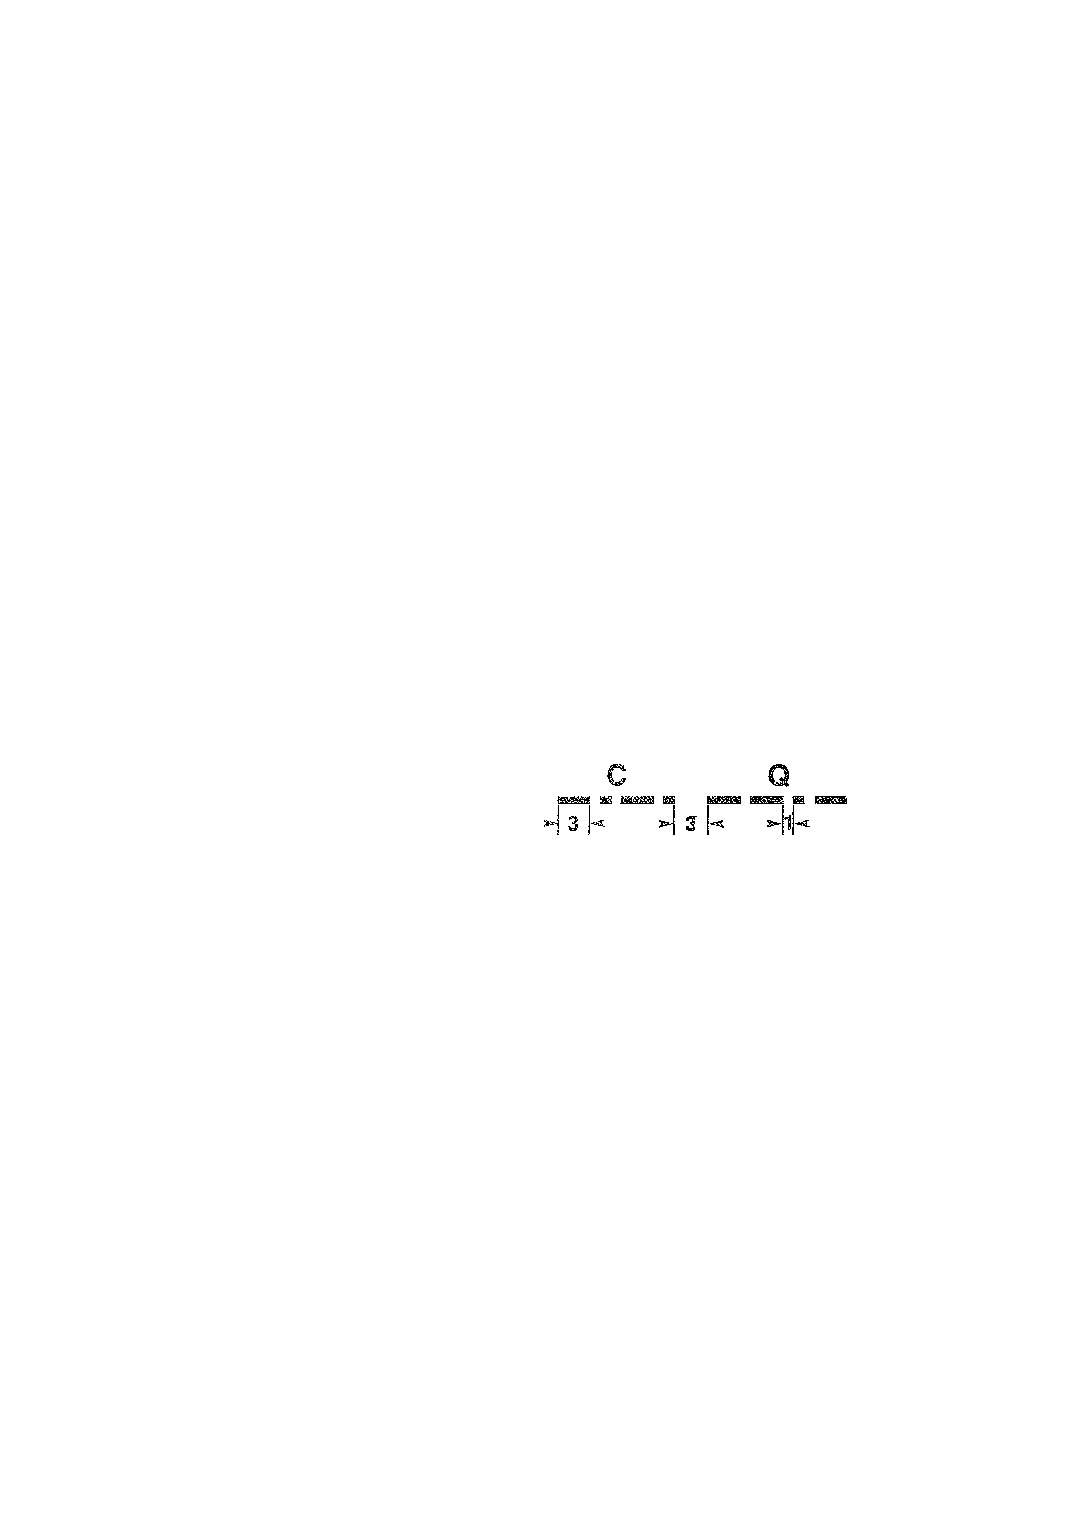
\includegraphics[width=0.5\textwidth]{images/bild_morse_1}}
  \caption{Morsetecknens uppbyggnad}
  \label{fig:bild_morse_1}
\end{wrapfigure}

Bild \ref{fig:bild_morse_1}.

Morsetecknen består av korta och långa teckendelar samt mellanrum. Man utgår från
den korta teckendelen vars längd sätts till en enhet. En lång teckendel ska
vara tre enheter lång, d.v.s. tre gånger längden av den korta
teckendelen. Mellan teckendelarna inom tecknet ska mellanrummet vara en enhet
långt. Mellan hela tecknen inom ord eller teckengrupp ska mellanrummet vara
tre enheter långt och mellan hela ord eller teckengrupper sju enheter långt.

\section{Planlagd övning}

Att delta i en organiserad kurs i den lokala radioklubben, FRO-avdelningen etc.
är bra, eftersom man då kan få en handledare och tillgång till övningsmaterial.
Inte minst viktigt är stödet av studiekamraterna. Det går också att på egen hand
lära sig att signalera, men det är ensamt och därför kanske lite svårare.
\begin{rev-omarbetas}
De kassettband och datadisketter som kan köpas från SSA kan användas i båda fallen.
\end{rev-omarbetas}

För att lära morsesignalering måste man vara motiverad. Det krävs nämligen
tålamod och regelbunden träning. Helst bör träningen ingå i den personliga dagliga
rutinen, även om det bara blir under några minuter. Det går att hoppa över 1-2
dagar i veckan, men det bör då ingå i övningsplanen. Att hoppa över ännu fler
blir lätt en ovana. Att träna lite då och då ger inget bra resultat.

\section{Ordning för teckeninlärning}

\begin{wrapfigure}[26]{R}{0.5\textwidth}
  \begin{tabular}{|r|l|}
    \hline
    \textbf{Lektion} & \textbf{Nya tecken} \\ \hline
    1 & = + L N E O \\
    2 & I X \\
    3 & V T \\
    4 & / ? + (vänta) \\
    5 & - x (repetition) \\
    6 & A Z \\
    7 & . (punkt) \\
    8 & H Ö \\
    9 & 7 4 9 5 \\
    10 & 8 1 \\
    11 & 3 6 \\
    12 & R D \\
    13 & 2 0 \\
    14 & F Y \\
    15 & Ä B \\
    16 & P S \\
    17 & U Q \\
    18 & W K \\
    19 & Å M \\
    20 & C G J \\
    21 & ~ (lystring) \\
    22 & @ (avslutning) \\
    23 & f (förstått eller felslagning) \\
    24 & ........ (felslagning) \\
    \hline
  \end{tabular}
  \caption{Inlärningsordning för morsetecknen}
  \label{fig:morse_ordning}
\end{wrapfigure}

Inlärningsordningen enligt bild \ref{fig:morse_ordning} rekommenderas. Man börjar med tecken som låter
så olika som möjligt. Detta för att undvika förväxling längre fram, när tecknen
blir fler och hastigheten högre. Under inlärningen blandas nya tecken med de
redan inlärda. Följ kursens ordning och hoppa inte över något! Öva utan avbrott,
så att hjärnan blir ordentligt ''programmerad''. Det är lämpligt att lära in 2
till 4 nya tecken varje vecka.

SSA:s telegraferingskurser på band och datadiskett har denna inlärningsordning.
Det finns dock kurser med annan uppläggning.

\hilight{TODO: Kolla upp status på SSA:s ''kurser på band och datadiskett''.}

\section{Inlärningstid}

Behövlig inlärningstid är mycket individuell. För ett UC-certifikat (40
tecken/minut), vilket är ett utbildningscertifikat från SSA, bör man räkna med
åtminstone 100 effektiva timmar för mottagning och 25 timmar för sändning.

Att klara CEPT 1-certifikatet innebär en taktökning till 60 tecken/minut och
högre krav på säkerhet i både mottagning och sändning, För det bör man räkna med
ytterligare 25 timmar eller mer.

\section{Inlärningsmetodik}

Morsetelegrafi bör läras med beprövad metodik. Bästa sättet är att man också
skriver ner tecknen när man hör dem. Metoden är s.k. ''nervbaning'' med målet att
handen reflexartat skriver ett visst tecken då en viss rytm hörs. Att träna bara
genom att höra tecknen är nästan verkningslöst. Först när Du lärt dej alla
morsetecken grundligt genom mottagning är det dags med sändningsträning.

\section{Mottagnings\-övningar}

Morsetecken är ju långa och korta teckendelar i form av ljud, ljus etc. De kan
även illustreras som långa och korta streck. För att tecknen ska uppfattas som
en melodi eller ljudföljd och för att man inte ska frestas att räkna korta
eller långa teckendelar är lämpligt att morsetecknen lärs in i hög hastighet,
men med förlängt mellanrum, s.k. spärrad stil. Det är själva ljudbilden som
ska läras in. I början kan det ändå vara svårt att låta bli att räkna
teckendelar, men efterhand uppfattar man trots allt tecknen som ljudbilder.

När man ska skriva mycket under en längre tid är sittställningen viktig. För
att inte bli trött ska man försöka inta en avslappnad sittställning och låta
hela underarmen vila mot bordet. Använd papper med stora rutor och en bra
kulspetspenna. Skriv gärna på varannan rad så att det finns plats under att
rätta texten.

För att spara tid bör man använda små handrörelser och inte lyfta pennan mer än
nödvändigt. studera skrivanvisningarna i slutet av detta kapitel. Använd för
tydlighetens skull textad stil, men tydlig skrivstil går också bra. Lyssna på
hela tecknet innan du skriver ner det. Skriv lugnt. Hoppa över tecken som du
missar! Försök inte att minnas tecken som du just missat. Då kommer du nog att
missa efterföljande tecken också. Koncentrera dig i stället på tecknen som
kommer.

Vissa morsetecken är så korta att det är svårt att hinna skriva ner dem. För att
spara tid måste vissa tecken skrivas i ett penndrag, t.ex. bokstäverna M, N m.
fl.. Bokstaven E som är det kortaste tecknet skriver man som en bakvänd trea
( \reflectbox{3} ). Bokstaven U bör formas fyrkantig och bokstaven V spetsig, annars
förväxlas de lätt. En nolla skrivs som Ø, med genomstrykning och en etta som 1.
En nolla utan streck kan lätt förväxlas med bokstaven O och en etta utan fot med
bokstaven I.

Var noga med handstilen från början och jobba hela tiden med att förbättra den.
En olämpligt inlärd handstil är mycket svår att arbeta bort och då får man
problem vid högre hastigheter. Du ska ju själv kunna tyda din text i
efterhand, men viktigast är att provförrättaren också ska kunna läsa den.

Inlärningstexter är ofta uppdelade i grupper med 5 eller 4 tecken. Dessa ska
simulera ord. Var noga med att du får tydliga ordmellanrum även på papperet.

\section{Eftersläpning vid mottagning}

Tiden för vart och ett morsetecken varierar kraftigt. För att få en lugnare
nedskrivning bör man försöka hålla några tecken i minnet och släpa efter med
nedskrivningen. Detta är nödvändigt i högre hastigheter och särskilt vid vissa
teckenkombinationer.

\emph{Läs inte!} Det är frestande att försöka bilda ord av de bokstäver som man
just skrivit ner. Läsningen tar bort uppmärksamhet från mottagningen och det
blir lätt felgissningar. Man tappar lätt den text som man just då tar emot. Läs
alltså inte och gissa inte på orden. Täck över det skrivna med den lediga
handen!

\section{Sändningsövningar}

Att telegrafera är att uttrycka sig. De handsända morsetecknen ska vara
tydliga, på samma sätt som att tal och vanlig handskrift ska vara det. Det är
därför mycket viktigt att teckengivningen lärs in på rätt sätt. Speciellt de
första sändningsövningarna bör ske tillsammans med en kunnig instruktör. Om
instruktör saknas -- följ då noga anvisningarna och var självkritisk!

\section{Hjälpmedel vid sändningsövning}

\hilight{TODO: Kolla upp det här programmet och om det fortfarande finns tillgängligt.}

För sändningsövningarna behövs en kassettbandspelare eller en dator med SSA:s
dataprogram ''Träna Morse''. Vidare behövsen summer ansluten till en
telegrafnyckel och en stereohörtelefon. Eventuellt kan man ha en andra summer
som nycklas av datorn och vars ljud matas i en av hörlurarna.

Lär in sändning med en manuell telegrafnyckel och inte med en s.k. bug. Vid
provtagning blir man nämligen ofta nervös och då är det lätt att sända fel med
en bug. Särskilt med en el-bug är risken stor för nya fel ''bara för att man
råkat snudda vid fel paddel''.  Vid rättning med bug kommer därför sällan ett fel
ensamt.

\section{Arbetsställning vid sändning}

Bild \ref{fig:bild_morse_3_4}

\begin{figure}
  \fbox{
    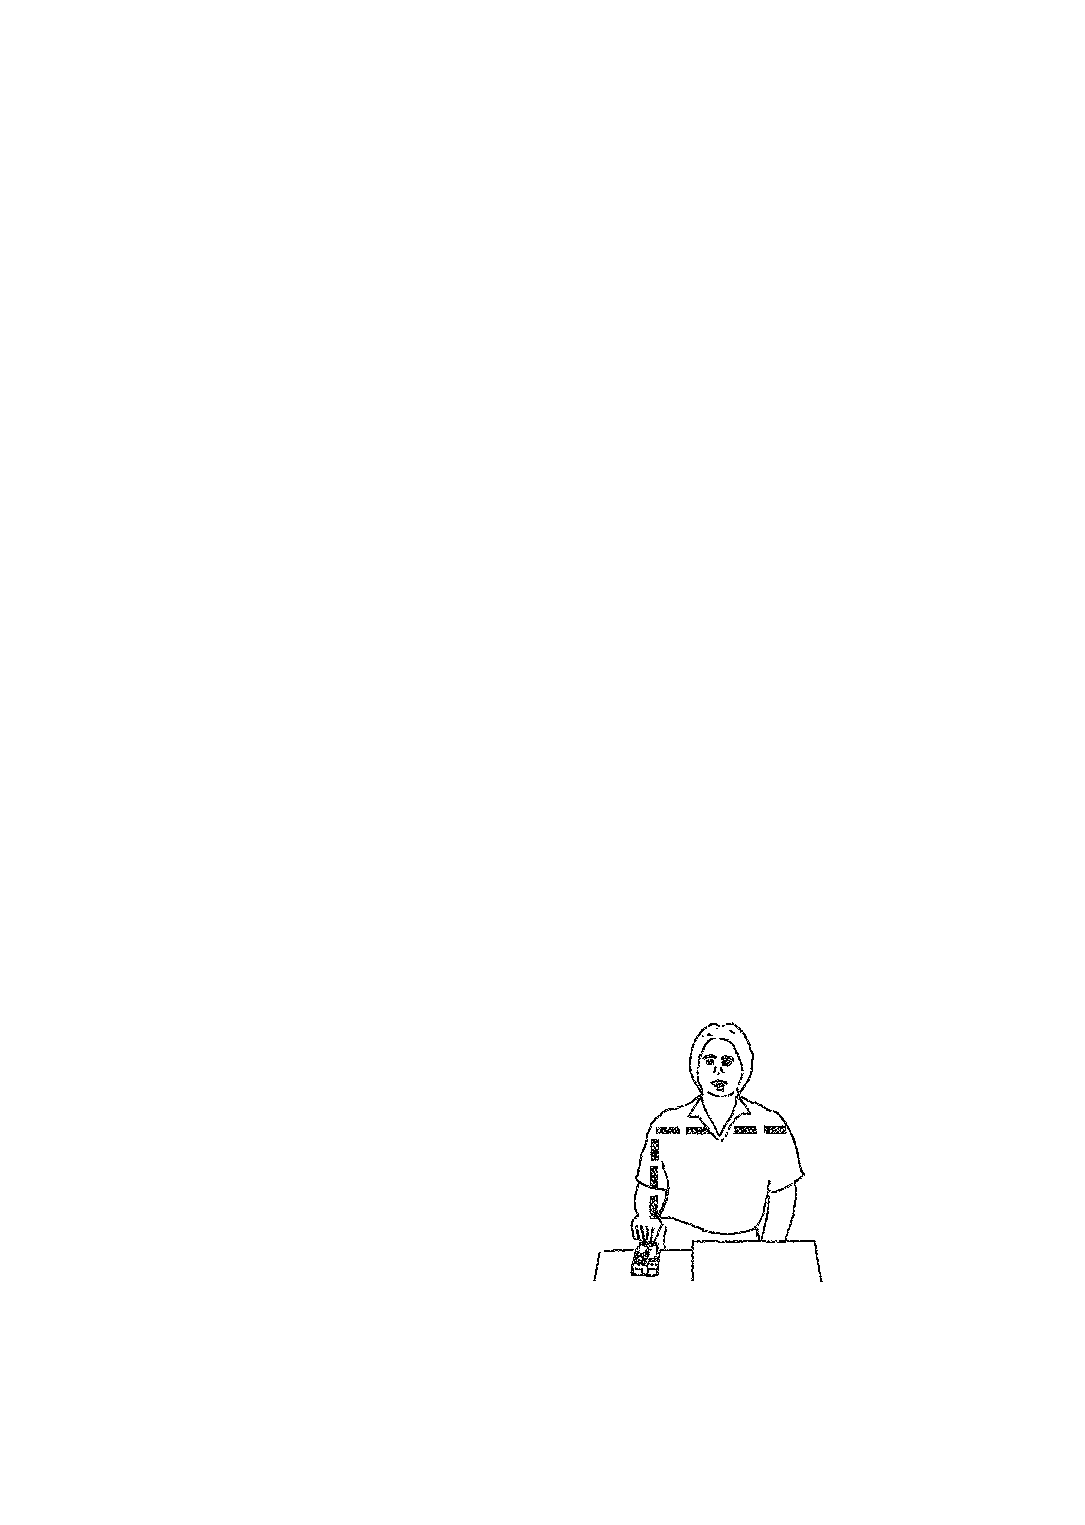
\includegraphics[width=0.5\textwidth]{images/bild_morse_3}
    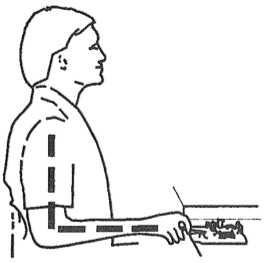
\includegraphics[width=0.5\textwidth]{images/bild_morse_4}
  }
  \caption{Rätt sittställning sett framifrån och från sidan}
  \label{fig:bild_morse_3_4}
\end{figure}

Det är viktigt att ha rätt arbetsställning redan från början. Vid hög
sändningstakt och långa sändningspass blir man annars lätt trött och får dålig
teckengivning.  Över 60-takt börjar rätt arbetsställning att få stor betydelse.

Vid trötthet under sändning höjer man ofta axeln varvid armbågen åker ut. Det
blir då arbetsamt och man får ''bryta sig'' genom slutet på texten under dålig
teckengivning.

Sitthöjden bör vara så att båda fötterna kan vila på golvet eller på en fotpall.
Telegrafnyckeln bör placeras så, att underarmen är vågrät när handen vilar på
nyckelknoppen. Överarmen kan då hänga avslappnad rakt nedåt och över- och
underarmen kan bilda en rät vinkel.

Nyckeln bör vara fastsatt. Det är tyvärr vanligt, att nyckeln ställs löst på ett
olämpligt högt bord. Detta medför en olämplig och tröttande arbetsställning.

\section{Nyckelfattning och handrörelser}

\begin{wrapfigure}{R}{0.5\textwidth}
  \fbox{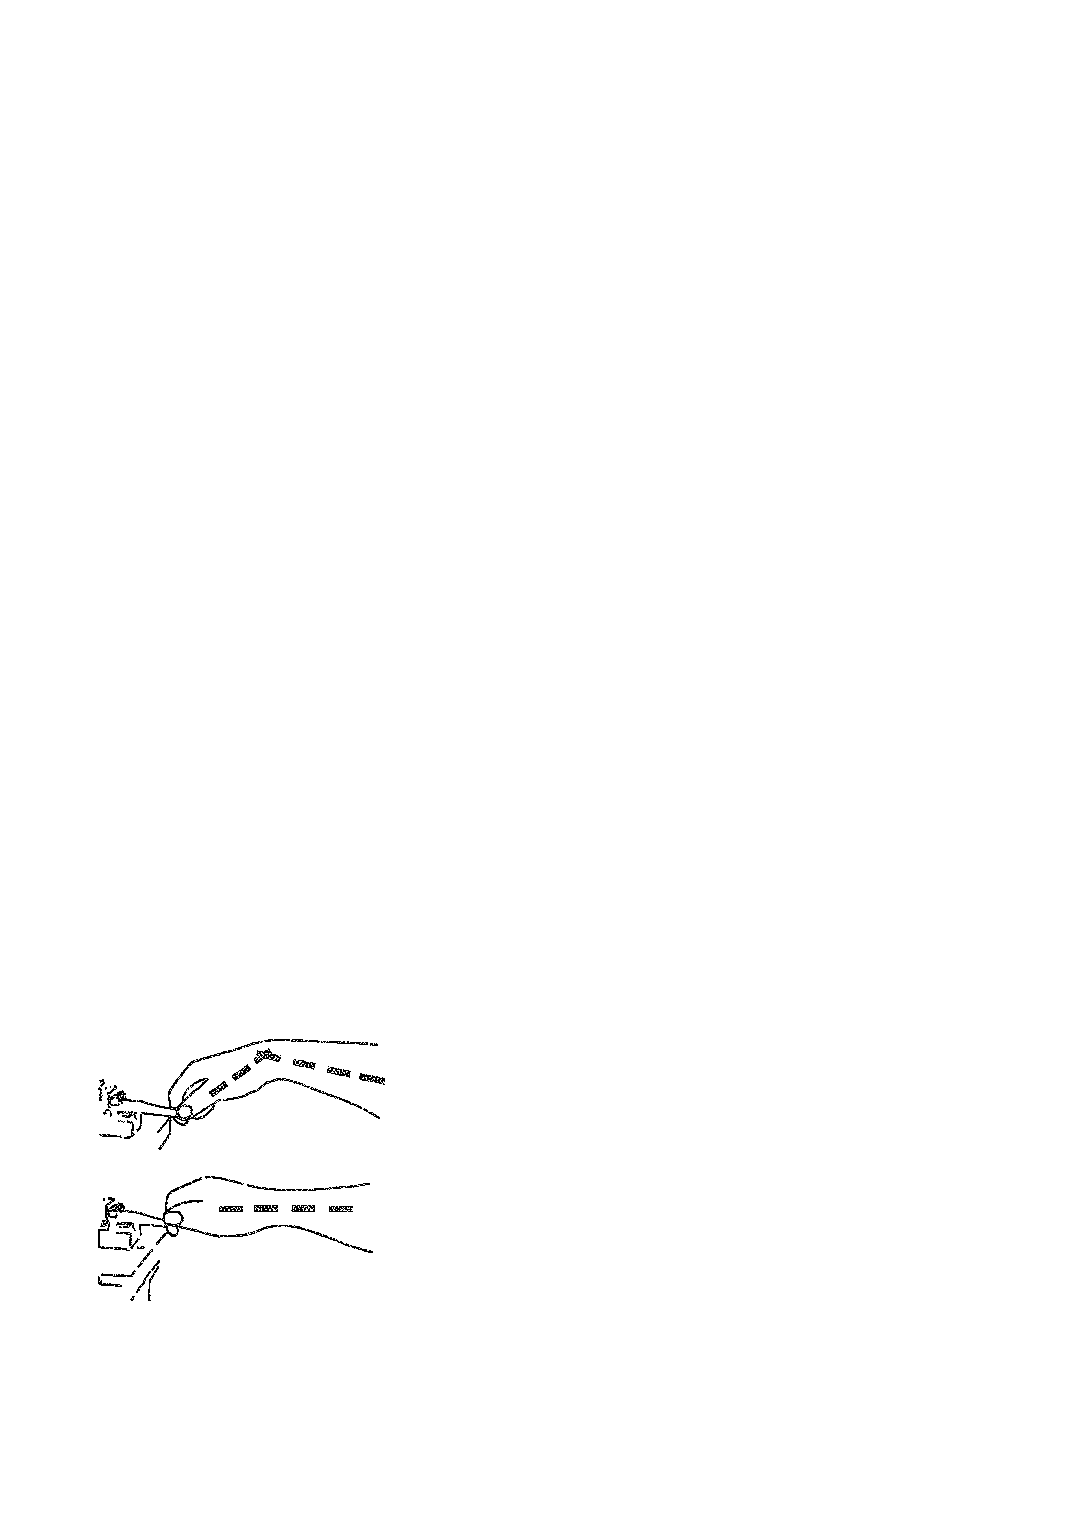
\includegraphics[width=0.5\textwidth]{images/bild_morse_5}}
  \caption{Rätta handledsrörelser}
  \label{fig:bild_morse_5}
\end{wrapfigure}

Bild \ref{fig:bild_morse_5}.

Håll löst omkring nyckelknoppen med tummen och långfingret. Pekfingrets
undersida ska vila lätt ovanpå knoppen. Använd alltid denna
trefingerfattning. Håll nyckelknoppen ganska långt in på fingrarna. När man
senare vill öka takten kan man flytta ut fattningen mot fingerspetsarna.

Morsetecknen skapas med rytmiska handledssvängningar uppåt/nedåt. Håll inte hårt
om knoppen -- men släpp den inte heller -- och spänn inte handleden. Handleden
ska svänga mellan ett något upplyft och ett vågrätt läge. I det vågräta läget
når nyckeln sitt s.k. kontaktläge. För att nästa tecken ska hinnas med i tid,
får handleden inte svänga djupare än till det vågräta läget.

\section{Styrd sändning}

Sändningsövningarna börjar med styrd sändning, men först sedan morsetecknen
lärts in grundligt genom lyssning. Vid styrd sändning använder man
stereohörlurar så att datorns eller bandspelarens sändning hörs i den ena luren
och den egna sändningen i den andra. Den ton som nycklas hämtas från en
generator som avger en konstant ton.

En textutskrift används som förlaga för den egna sändningen. Det gäller att
lyssna på morsetecknen från datorn eller bandet, samtidigt läsa samma tecken
från utskriften och själv sända dessa med nyckeln. Ljudbilden från en egna
sändningen ska då sammanfalla med den från förebilden. På så sätt samövas
hand- och armmusklerna, synen och hörseln för rätt teckengivning.

I SSA:s kurser på ljudband och data finns rytmiska ramsor för övning av styrd
sändning. Börja med att öva ramsorna i nummerordning. När man blir säkrare
behöver man inte alltid träna alla ramsor. Man känner själv vilka ramsor som man
behöver öva mera.

Styrd sändning övas utan spärrning. Teckenhastigheten och trafikhastigheten ska
då vara lika. Trafikhastigheten bör åtminstone vara 35 till45 tecken/minut för
attteckenrytmen ska bli bra. Träna mycket på siffror i den styrda
sändningen. Det ger färdighet vid övergångarna mellal korta och långa
teckendelar i tecknen. Även mellan vissa morsetecken kan övergångarna vara
svåra.

\section{Fri sändning}

Först ska styrd sändning av ramsor och tecken klaras utan problem. Börja först
därefter med fri sändning utan ljudförebild. Normalt ska sändning göras utan
spärrning.

Försök komma ihåg teckenrytmen från den styrda sändningen. Siffror och
skiljetecken är svårast att sända. Öva därför dessa tecken extra mycket. Då blir
också bokstäverna lättare att sända!

Sänd inte fortare än att handleden fortfarande arbetar mjukt vid kontaktläget,
men ändå distinkt. Sändningen är ditt visitkort och därför krävs att den har
kvalitet.

\begin{figure}
  \fbox{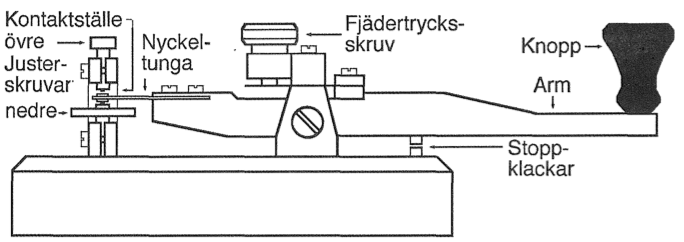
\includegraphics[width=\textwidth]{images/bild_morse_6}}
  \caption{Telegrafnyckel}
  \label{fig:bild_morse_6}
\end{figure}

\section{Kontroll av teckengivningen}

Läsbarheten av den sändningsstil, som uppvisas vid certifikatsprovet,
bedöms. Ett i övrigt godkänt prov kan alltså bli underkänt p.g.a. dålig
teckengivning. Återkalla därför ett tveksamt utformat morsetecken och sänd om
det, men var då klar över att provtexten ökar med det antal tecken man sänder
om. Det innebär tidsförlust.

För kontroll av teckengivningen under sändningsprovet, och registreringen av
det, användes förr en teckenskrivare med pappersremsa. Emellertid är en sådan
skrivare numera ett svåråtkomligt hjälpmedel.

Det hjälpmedel, som i stället står till buds, är en ljudbandspelare, men tyvärr
har ju en sådan inte grafisk visning. En telegraferingskunnig person bör därför
anlitas för bedömning av teckengivningen.

\section{Exempel på provtext}

.... ASCUNCION ÄR HUVUDSTAD I PARAGUAY, SOM LIGGER I SYDAMERIKA.  VID
RADIOTELEFONERING UTGÖRES NÖDSIGNALEN AV ORDET MAYDAY OCH SKALL OM MÖJLIGT
UTSÄNDAS PÅ FREKVENSEN 2182 KHZ. QRV? MEANS ARE YOU READY? THE RECEIVER CONTROL
SETTINGS SHOULD BE ADJUSTED AS INDICATED ON PAGE 3-4, DATED 7/10 1994. QRT + @
(summa 277 teckenvärden)

\section{Beräkning av antalet teckenvärden}

Vid beräkning av antalet teckenvärden i en telegramtext ska bokstäver (utom Å)
räknas som ett (1) teckenvärde. Siffror, skiljetecken, felsändningstecken samt
bokstaven Å ska räknas som två (2) teckenvärden.

I ovanstående exempel på provtext är fördelningen av teckenvärdena följande:

\begin{tabular}{lrcrcr}
Bokstäver          & 1 & $\cdot$ & 227 & = & 227 \\
Siffror            & 2 & $\cdot$ & 13  & = & 26  \\
Skiljetecken       & 2 & $\cdot$ & 12  & = & 24  \\
Summa teckenvärden &   &         &     & = & 277
\end{tabular}

Observera, att lystrings-, slut- och avslutningstecken samt felsända avsnitt med
respektive felsändningstecken också ska ingå i summan av teckenvärden.

Den därefter beräknade takten är den s.k. telegram- eller trafikhastigheten.

\section{Beräkning av takten}

Formel:

$$\frac{\mathrm{summa\ teckenv"arde }\cdot 60}{\mathrm{tid} [\mathrm{sekunder}]}
= \mathrm{tecken/min}$$

Exempel: Felfri sändning av ovanstående exempel på provtext med summa
teckenvärde 277 tar exakt 4 minuter och 20 sekunder (260 sekunder). Takten blir
då:

$$\frac{277 \cdot 60}{260} = 63,9\ \mathrm{tecken/min}$$

\begin{figure}
  \fbox{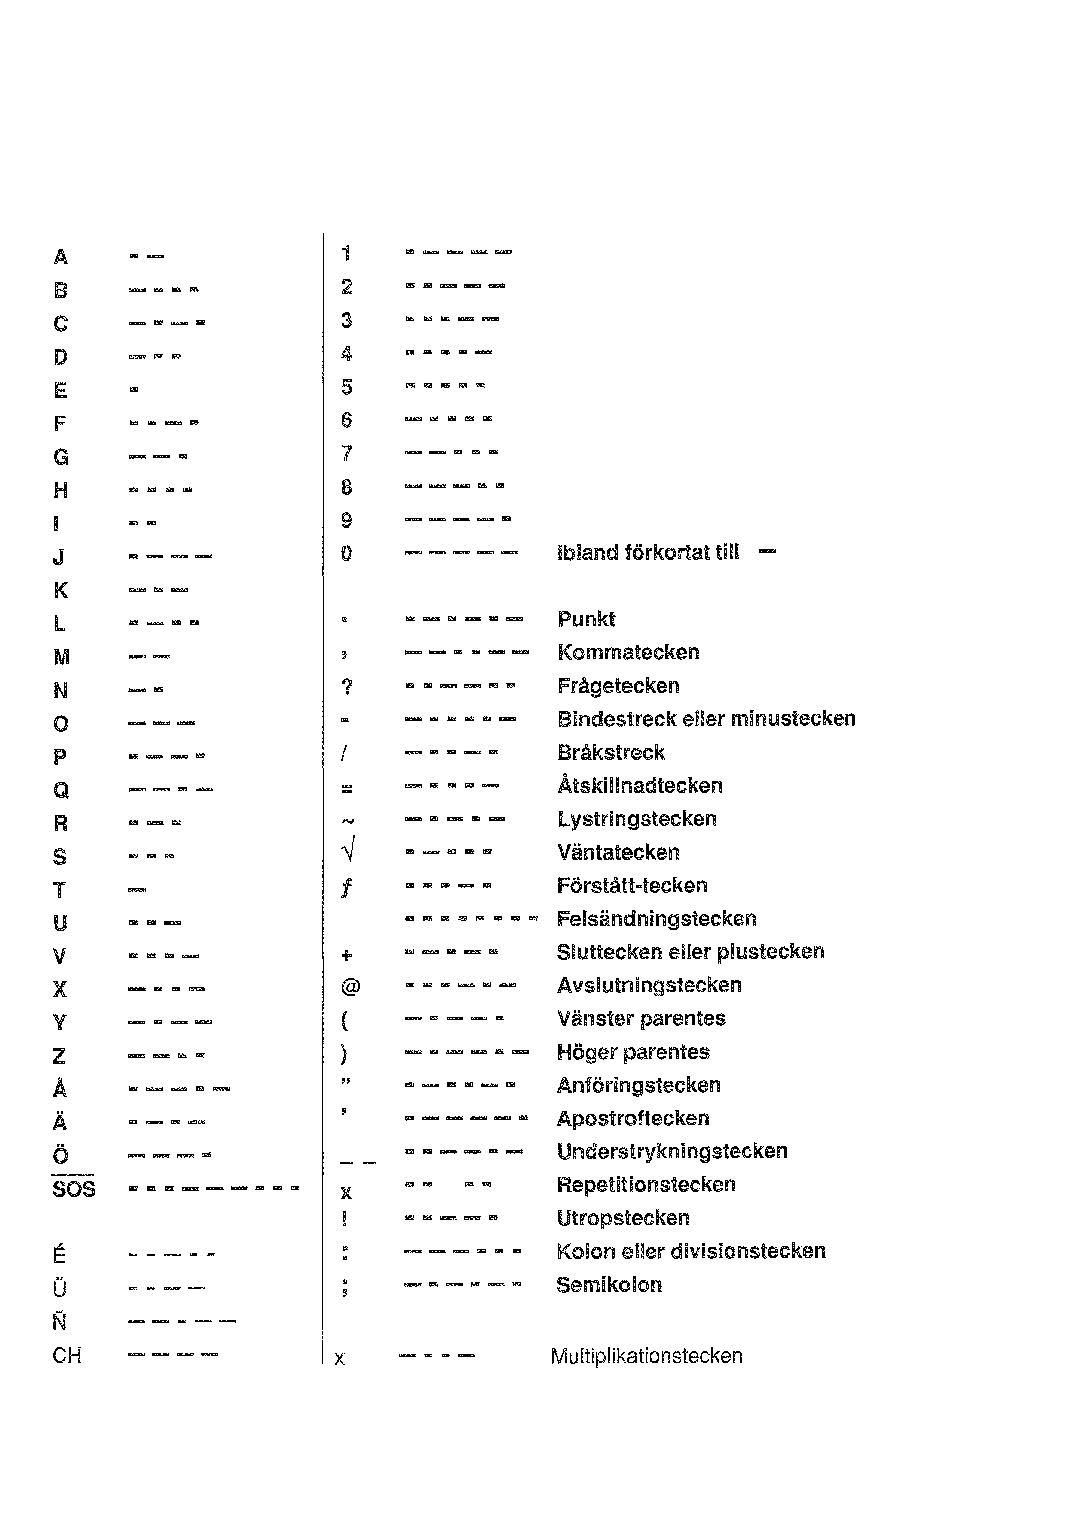
\includegraphics[width=\textwidth]{images/bild_morse_7}}
  \caption{Handstilar}
  \label{fig:bild_morse_7}
\end{figure}

\begin{figure}
  \fbox{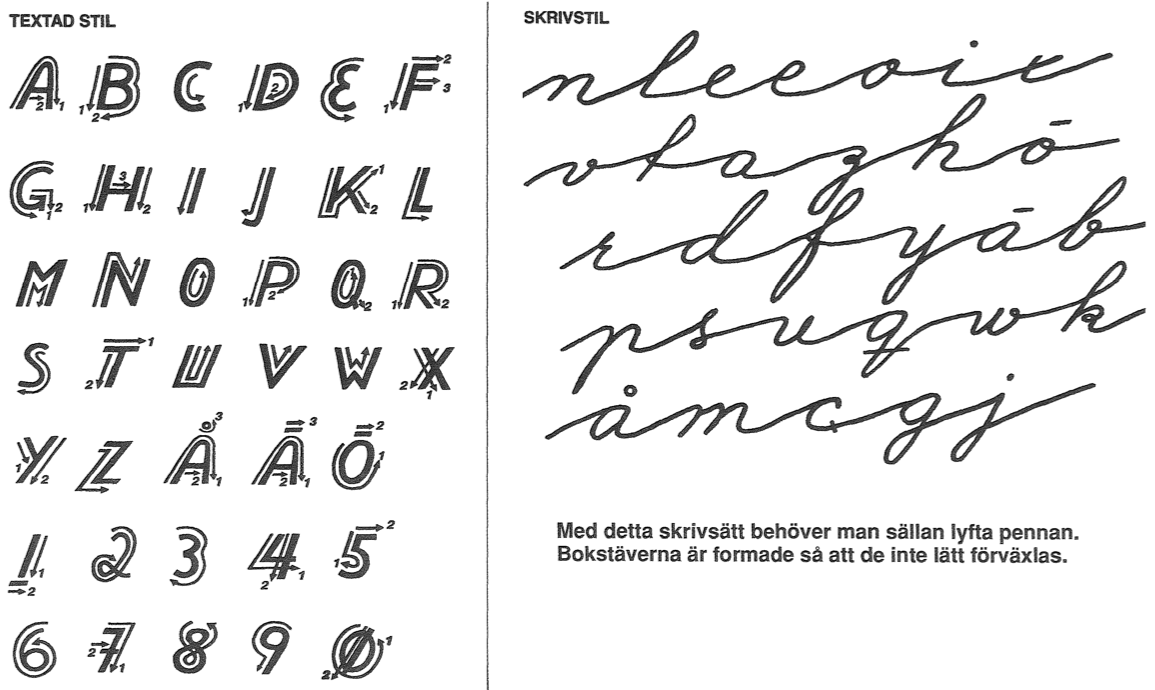
\includegraphics[width=\textwidth]{images/bild_morse_8}}
  \caption{Handstilar}
  \label{fig:bild_morse_8}
\end{figure}


%\part{RADIOTEKNIK}


%\chapter{El-lära}

%\chapter{Ellära}
\label{ellära}

\section{Elektriska grundbegrepp}

\harec{a}{1.1}

Elektrisk laddning, spänning och ström hänger samman med hur materian är
uppbyggd.
Den förmåga ett material har att leda laddningar, dvs. ström, kallas
konduktivitet.

\subsection{Grundämnen}
\textbf{FÖRDJUPNING}
\index{grundämnen}

Det finns många former av materia.
Ofta är en form av materia sammansatt av andra former med enklare uppbyggnad.

Sammansatt materia kan sönderdelas på kemisk väg, men däremot inte de enklaste
formerna.
All materia är uppbyggd av atomer.
De enklaste materieformerna, som kallas \emph{grundämnen}, innehåller endast
ett slags atomer.
Över 100~grundämnen är kända.

Vart och ett av grundämnena har sin speciella atomuppbyggnad och därmed en
materialstruktur, som skiljer sig från varje annat grundämne.

Tre fjärdedelar av alla grundämnen är metaller (elektriska ledare) medan de
flesta övriga är icke-metaller (isolatorer).
Det finns även en liten mellangrupp som kallas för halvledare.

\subsection{Atomernas uppbyggnad}
\textbf{FÖRDJUPNING}

Länge ansågs atomerna vara de minsta beståndsdelarna i materian.
Men omkring förra sekelskiftet upptäcktes att atomerna i sin tur består av ännu mindre
beståndsdelar, s.k. elementarpartiklar såsom protoner, neutroner, elektroner
m.fl.
Det gemensamma namnet för alla dessa partiklar är \emph{nukleoner}.

En atom består dels av en kärna som är sammansatt av protoner och neutroner,
dels av elektroner, som kretsar omkring kärnan.

\begin{quote}
\emph{Protonerna är positivt (+) laddade.}

\emph{Neutronerna är neutrala, ej laddade.}

\emph{Elektronerna är negativt (-) laddade}
\end{quote}

\begin{wrapfigure}{L}{0.5\textwidth}
  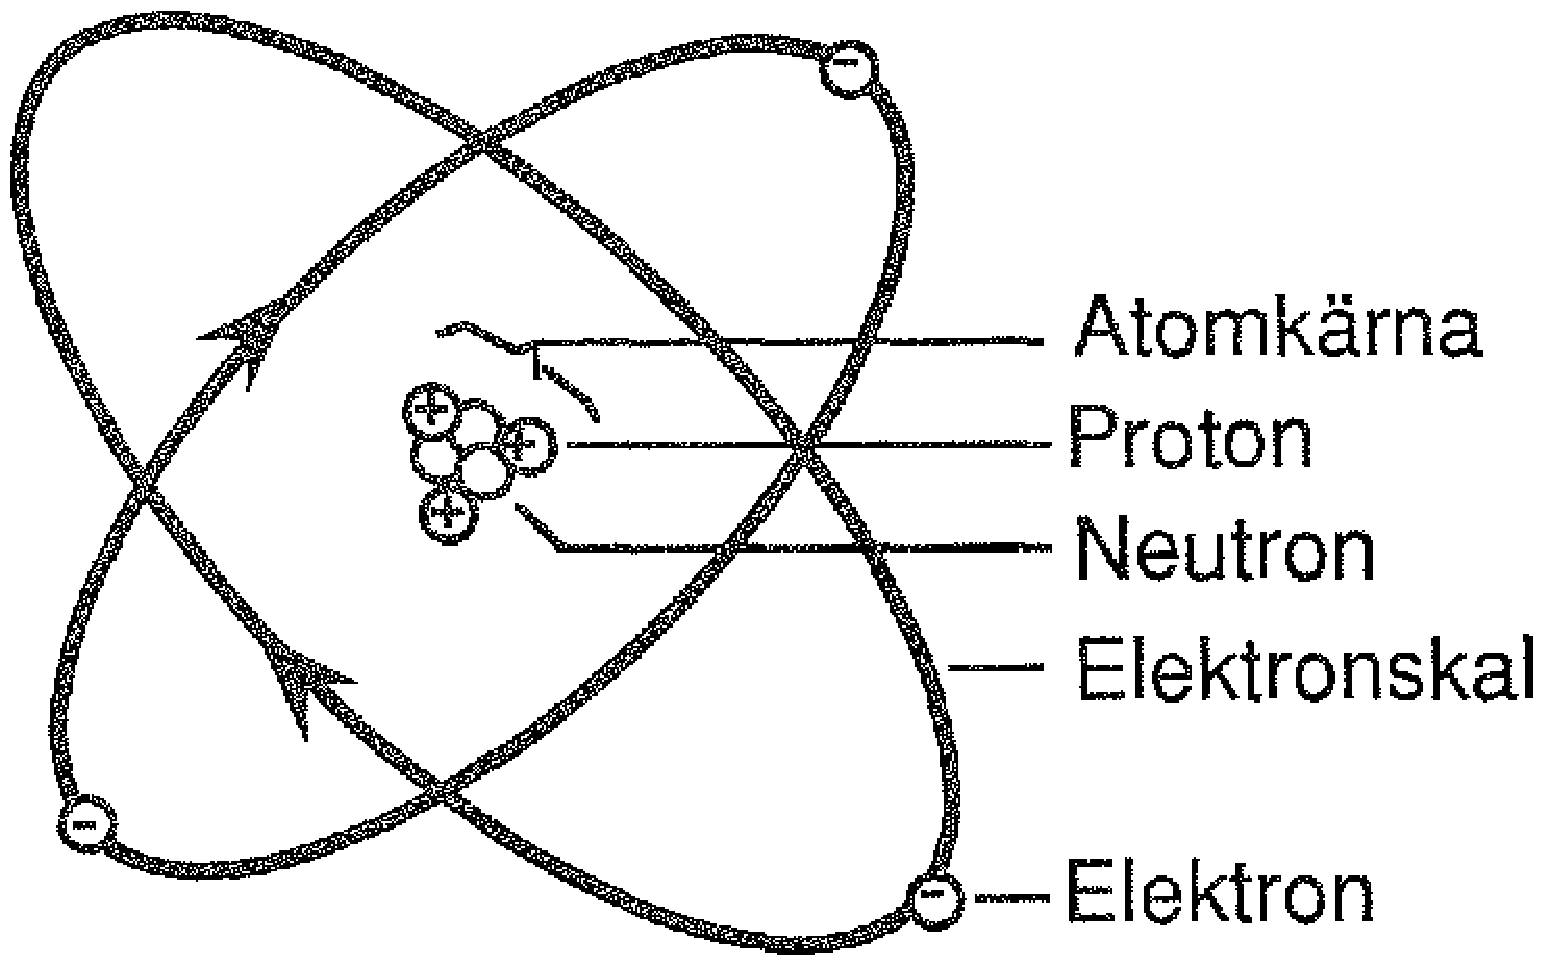
\includegraphics[width=0.5\textwidth]{images/cropped_pdfs/bild_2_1-01.pdf}
  \caption{Atomernas uppbyggnad}
  \label{fig:BildII1-1}
  \vspace{-20pt}
\end{wrapfigure}

Elektronerna kretsar i banor omkring atomkärnorna, liksom
planeterna kretsar i banor omkring sina solar, vilket illustreras i bild
\ref{fig:BildII1-1}.

Banor med samma avstånd till atomkärnan är på samma energinivå och sägs bilda
ett elektronskal.

Det kan finnas flera elektronskal.
Ju fler elektroner som finns i ett elektronskal, desto starkare är elektronerna
i skalet bundna till atomen.
Det yttersta skalet kan emellertid aldrig innehålla fler än 8~elektroner.

Elektronerna i det yttersta skalet kallas för \emph{valenselektroner}, vilka
används även av angränsande atomer vid den kemiska bindningen till
atomstrukturer, molekyler och ämnen.
För bindningen behövs ett visst antal valenselektroner.

De valenselektroner som ej behövs för bindningen kan röra sig fritt genom
materia/strukturen.
De kallas fria elektroner och är vad vi kallar elektrisk ström.

Valenselektronerna är alltså inte bara av betydelse för materialets kemiska
struktur utan också för dess elektriska egenskaper.

Atomernas massa och volym är ytterst liten.
Tag som exempel en kub av koppar med volymen \(1\ cm^3\) och vikten
\(8,9\ gram\).
Den består av ca \(8,5 \cdot 10^{22}\) kopparatomer, dvs.
\(85\, 000\, 000\, 000\, 000\, 000\, 000\, 000\) stycken.
Fenomenet metallbindning gör att antalet fria elektroner i kuben är ungefär lika
med antalet atomer i den.

Varje elementarpartikel har en massa och en atoms totala massa är summan av
elementarpartiklarnas massor.
Den enklaste atomen är väteatomen med en proton och en elektron.
Väteatomens totala massa har kunnat beräknas till \(1,66 \cdot 10^{-24}\) gram.

Nästan hela massan i atomen är samlad till kärnans protoner och neutroner.
Var och en av dem har en massa som är ungefär 2000 gånger större än massan i en
elektron.

\subsection{Elektrisk laddning och kraftverkan}
\textbf{FÖRDJUPNING}
\index{elektrisk laddning}

Enligt sägnen upptäckte Thales från Milteus redan för 2500~år sedan, att en bit
bärnsten drog till sig små grässtrån, sedan stenen gnidits mot en bit ylle.
Det grekiska ordet för bärnsten är ELEKTRON och de krafter som uppstod kom att
kallas ''elektriska''.
Av den elektriska spänningen mellan kroppar med olika laddning, verkar krafter
mellan dem och deras omgivning.
Krafterna kallas för elektriska fält och är det som gör att elektriskt laddade
kroppar kan komma i rörelse.

Ett exempel får man varje gång man kammar sig med en kam av isolerande material.
Då kommer håret att dras mot kammen därför att håret och kammen har
fått olika slags elektriska laddningar.
Samtidigt har hårstråna sinsemellan samma slags laddning och stöter bort
varandra -- håret ''reser sig''.

Lika laddningar stöter bort varandra.

Olika laddningar drar varandra till sig.

\subsection{Konduktivitet -- Ledare, halvledare och isolator}
\textbf{HAREC a.\ref{HAREC.a.1.1.1}\label{myHAREC.a.1.1.1}}
\index{konduktivitet}

En elektrisk ström sägs flyta, när de fria laddningsbärarna i ett material -- en
strömledare -- fås att röra sig samtidigt i samma riktning.
Hur många som rör sig beror på strömledarens egenskaper och spänningen mellan
ledarens ändar.

Alla material har någon grad av elektrisk ledningsförmåga som beror på
materialets atomstruktur, dimensioner och temperatur.
Vissa material (t.ex. metaller, kol, halvledare) leder elektrisk ström bättre
än andra (t.ex. glas, gummi, plast).
Mängden av fria laddningsbärare i materialet begränsar hur stor strömmen kan
bli.

\subsubsection{Ledare}
\index{ledare}
\index{konduktivitet!ledare}

Metaller har god elektrisk ledningsförmåga och kallas ledare.
Bäst ledande är de metaller, vars atomer har det minsta antalet
valenselektroner i det yttersta elektronskalet.
Koppar-, silver- och guldatomerna har en enda valenselektron och därmed mycket
god ledningsförmåga.
Järn, zink och magnesium har två valenselektroner och därmed något sämre
ledningsförmåga.
Ännu sämre ledare är de s.k. halvledarna med 3 till 5 valenselektroner.

\subsubsection{Isolatorer}
\index{isolator}
\index{konduktivitet!isolator}

Glas, plast, porslin och vissa mineraler har mycket dålig ledningsförmåga och
kallas isolatorer.
Isolatorerna är dåliga ledare på grund av att de har många valenselektroner i
sitt yttersta skal.
Maximalt ryms 8 valenselektroner.

I icke ledande material är elektronerna mycket hårt bundna till sitt valensskal
och därför svåra att flytta.
I fasta material är också positiva laddningar svåra att flytta, eftersom de är
bundna i atomkärnorna.
Atomerna är i sin tur bundna i en struktur som kännetecknar vart och ett
material.

\subsubsection{Halvledare}
\index{halvledare}
\index{konduktivitet!halvledare}

Några grundämnen har en elektrisk ledningsförmåga som ligger mellan gränsvärdena
för att kallas elektriska ledare eller isolatorer.
Dessa ämnen tillhör gruppen halvledande ämnen.
De halvledande ämnena har en elektrisk ledningsförmåga som varierar med ämnets
renhet och temperatur.

En ren kristall av mineralen germanium [Ge] eller av kisel [Si] bildar ett
kristallgitter där atomerna binds till varandra med kovalenta bindningar.
Ämnena delar sina fyra valenselektroner med fyra andra atomer så att det
bildas en full oktett med åtta elektroner i valensskalet.

Då valensskalet innehåller åtta elektroner är det fullt, det finns inga fria
elektroner och ämnet leder inte elektrisk ström.
Båda dessa mineraler är därför i denna form isolatorer.
(\emph{intrinsisk halvledare})

Om några atomer av ett främmande material som till exempel arsenik, antimon,
indium eller gallium blandas in (\emph{dopas}) i deras kristallstruktur, så blir
de i till viss del elektriskt ledande -- de blir halvledare.
Beroende på materialen och i vilka proportioner de blandas fås olika egenskaper.

Den halvledande förmågan är inte nämnvärt beroende av temperaturen utan styrs mer
av inblandningen av andra ämnen.
Detta gäller upp till cirka +85 \degree C för germanium och till +150 \degree C
för kisel.

\subsubsection{N-ledning}
Man talar om N-ledande material respektive N-ledning- ''elektronledning''.

Germanium, kisel m.fl. halvledare har fyra elektroner med ''fasta platser'' i
valensskalet -- förutsatt att materialet är helt rent.
Då finns det inga fria elektroner för laddningstransport.

För att skapa fria elektroner kan det rena materialet förorenas -- dopas -- med
atomer av t.ex. arsenik [As] eller antimon [Sb].
Båda dessa material är 5-värdiga.
De har 5 elektroner i valensskalet 4 elektroner är fast bundna medan
den 5:e är löst bunden till atomen.
Den 5:e elektronen kan lossgöras från atomen med yttre kraft, t.ex. värme eller
elektrisk spänning och då skapas en fri elektron.
När en spänning läggs på materialet kommer den fria elektronen att vandra mot
den positiva polen.
Materialet är N-ledande.

\subsubsection{P-ledning -- ''hålledning''}
När germanium eller kisel dopas med indium [In] eller gallium [Ga] blir de
P-ledande.
Indium och gallium är 3-värdiga -- deras valensskal innehåller 3 elektroner.
Men för en fast bindning med germanium eller kisel saknas det en elektron och
det uppstår då ett ''hål'' -- en ''bristelektron''.
Hålet kan fyllas ut av en elektron från en annan atom.
I den atom som elektronen lämnar bildas det i sin tur ett hål osv.
När en spänning läggs på, kommer ''hålet'' att vandra mot den negativa polen.
Materialet är då P-ledande.

\subsection{Elektrisk spänning -- Enheten volt}
\textbf{HAREC a.\ref{HAREC.a.1.1.2}\label{myHAREC.a.1.1.2b}, a.\ref{HAREC.a.1.1.3}\label{myHAREC.a.1.1.3b}}
\index{elektrisk spänning}
\index{spänning}
\index{volt (V)}
\index{enheter!volt (V)}
\index{symbol!\(U\) spänning}
\index{symbol!\(V\) spänning}

\begin{figure*}
\begin{center}
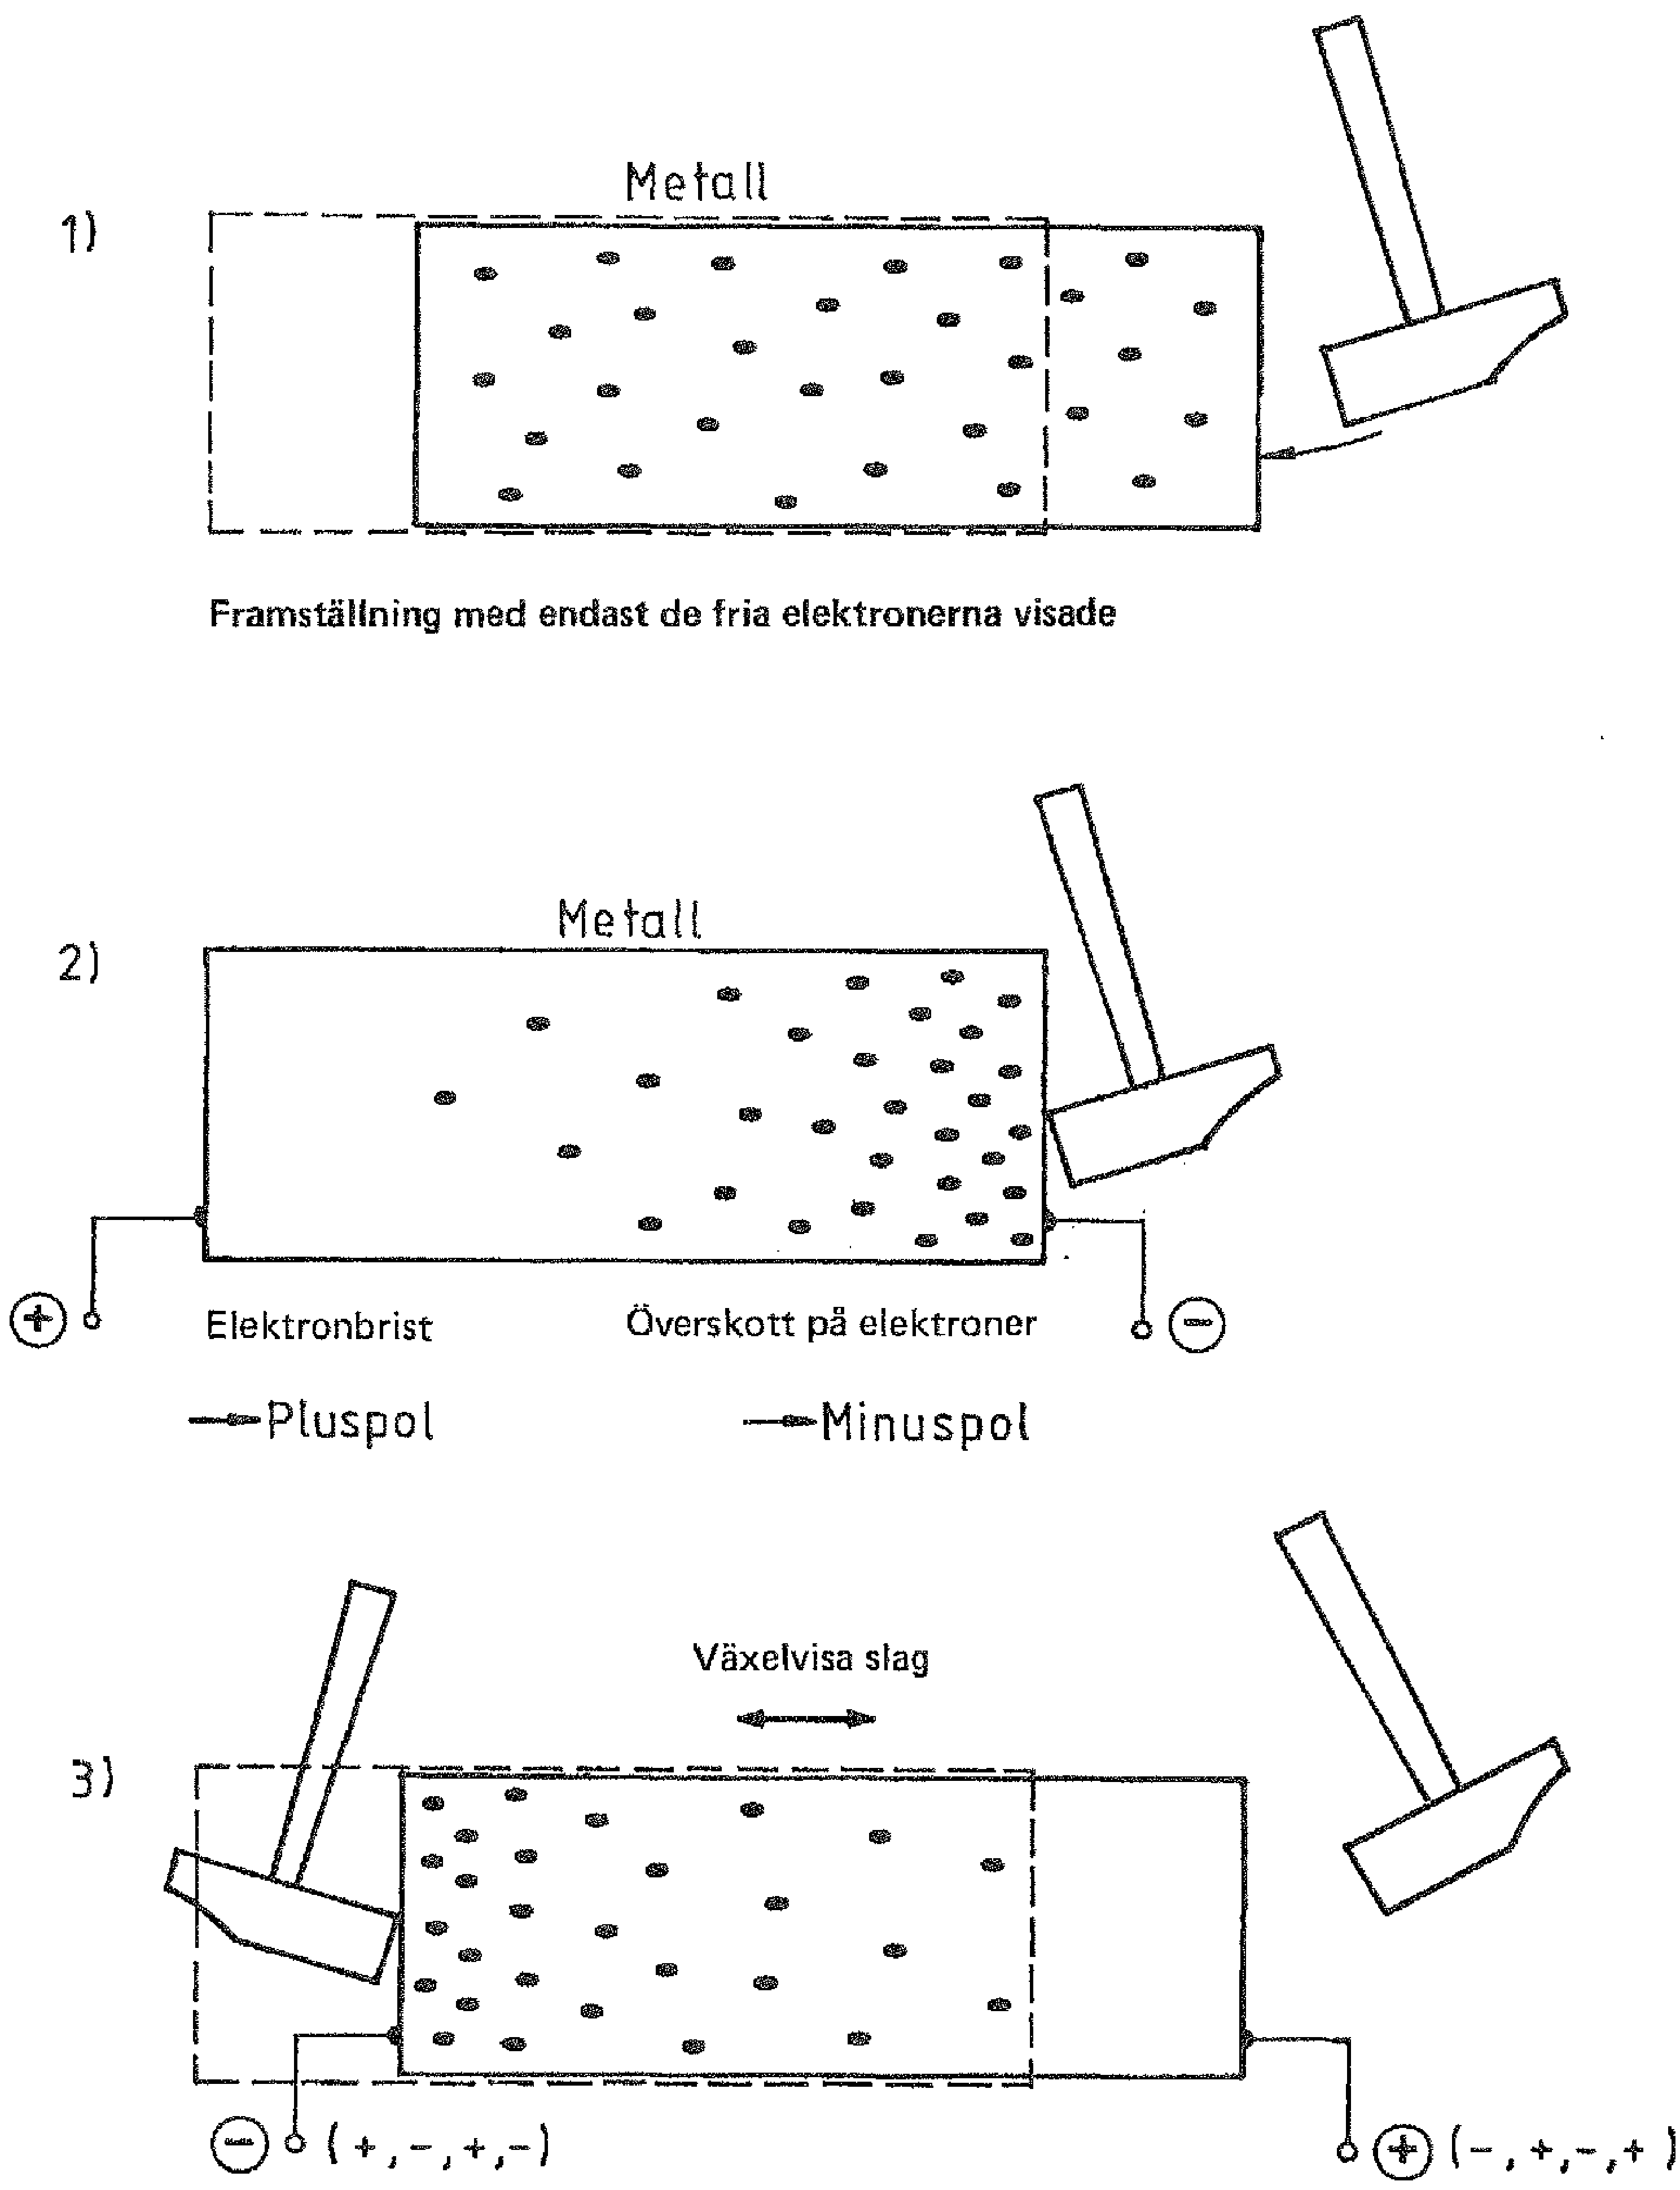
\includegraphics[width=\textwidth]{images/cropped_pdfs/bild_2_1-02.pdf}
\caption{Tankeförsök med kulor i ett rör}
\label{fig:BildII1-2}
\end{center}
\end{figure*}

Bild \ref{fig:BildII1-2} illustrerar ett tankeförsök med ett rör med kulor i. Materialet i röret tänks motsvara atomstrukturen i en strömledare och kulorna
de fria elektronerna.
Tänker man sig ett slag mot en ände av röret så flyttar det sig av den energi
som tillförs.
På grund av obundenheten till röret följer av masströgheten kulorna inte med
röret, utan hamnar i dess ena ände.

Att kulorna samlas i ena änden av röret tänks motsvara ett elektronöverskott i
ena änden av en ledare och ett motsvarande underskott i den andra änden.

Man kallar änden med elektronöverskott för minuspol och änden med
elektronunderskott för pluspol.
Olika stora elektriska laddningar vid polerna innebär att de sinsemellan har
olika potential.
Potentialskillnaden kallas spänning.

Likspänning innebär ett överskott av elektroner och alltid vid samma
anslutningspol.

Växelspänning innebär ett överskott av elektroner, omväxlande vid den ena
anslutningspolen och den andra.

Måttenheten för spänning är \(\mathrm{volt\ [V]}\).
I formler betecknas spänning med
\begin{itemize}
  \item \(U\) för effektivvärdet
  \item \(u\) för momentanvärdet (ögonblicks-)
  \item \(\hat{u}\) för toppvärdet (amplitud-).
\end{itemize}
Bild \ref{fig:BildII1-16} i avsnitt 1.6 illustrerar relationen mellan värdena
för en sinuskurva.

Spänningen över ändpunkterna på en strömledare är \(1\ \mathrm{volt\ [V]}\), då
ledaren genomflyts av en likström av \(1\ \mathrm{ampere\ [A]}\) under
effektutvecklingen \(1\ \mathrm{watt\ [W]}\).

\subsection{Symboler}

\begin{wrapfigure}[6]{R}{0.4\textwidth}
  \begin{mdframed}
    \centering
    \begin{circuitikz}
      \draw
      (4,1) to[battery1] (1,1)
      ;
    \end{circuitikz}
    \caption{Schemasymbol för batteri}
    \label{fig:bildII2-batteri}
  \end{mdframed}
\end{wrapfigure}

\textbf{FÖRDJUPNING}

När man ritar scheman för elektriska kretsar används symboler.
Symbolen i bild \ref{fig:bildII2-batteri} visar ett elektriskt batteri med en
enda cell.

Förtydligande kommentarer och skrivtecknen invid symbolen förekommer.
Ofta refererar dessa till en komponentlista.
Se även kapitel \ref{komponenter}.

\subsection{Elektrisk ström -- Enheten ampere}
\textbf{HAREC a.\ref{HAREC.a.1.1.2}\label{myHAREC.a.1.1.2a}, a.\ref{HAREC.a.1.1.3}\label{myHAREC.a.1.1.3a}}
\index{elektrisk ström}
\index{ström}
\index{ampere (A)}
\index{enheter!ampere (A)}
\index{symbol!\(I\) ström}

När en sluten strömkrets innehåller en spänningskälla, kan en
laddningsutjämning ske genom kretsen.
Det innebär att fria elektroner förflyttar sig genom kretsen i riktning från
spänningskällans minuspol till dess pluspol.
Vid pluspolen är det nämligen brist på negativa laddningar och naturen söker
alltid en utjämning.
Under utjämningsförloppet är spänningskällan även en strömkälla.

I gaser och elektrolyter (elektriskt ledande vätskor och geler) samt i
halvledare består strömmen av joner (positiva eller negativa laddningar), i metaller däremot av elektroner (negativa laddningar).

Av tradition anses strömriktningen vara positiv i jonströmmens riktning -- den
s.k. tekniska strömriktningen -- medan elektronströmmens riktning är den
motsatta -- den s.k. fysikaliska strömriktningen.

Måttenheten för ström är \emph{ampere} \(\mathrm{A}\) \cite{SIbrochure8}.

I formler betecknas ström med
\(I\) för effektivvärdet,\\
\(i\) för momentanvärdet (ögonblicks-),\\
\(\hat{i}\) för toppvärdet (amplitud-).

Strömmen är \(1\ \mathrm{A}\) när \(6,25 \cdot 10^{18}\) elektroner per sekund
flyter genom ett givet ledartvärsnitt, vilket motsvarar laddningen
\(1\ \mathrm{coulomb}\).

\subsection{Strömkrets}
\textbf{FÖRDJUPNING}
\index{strömkrets}

\begin{figure*}
\begin{center}
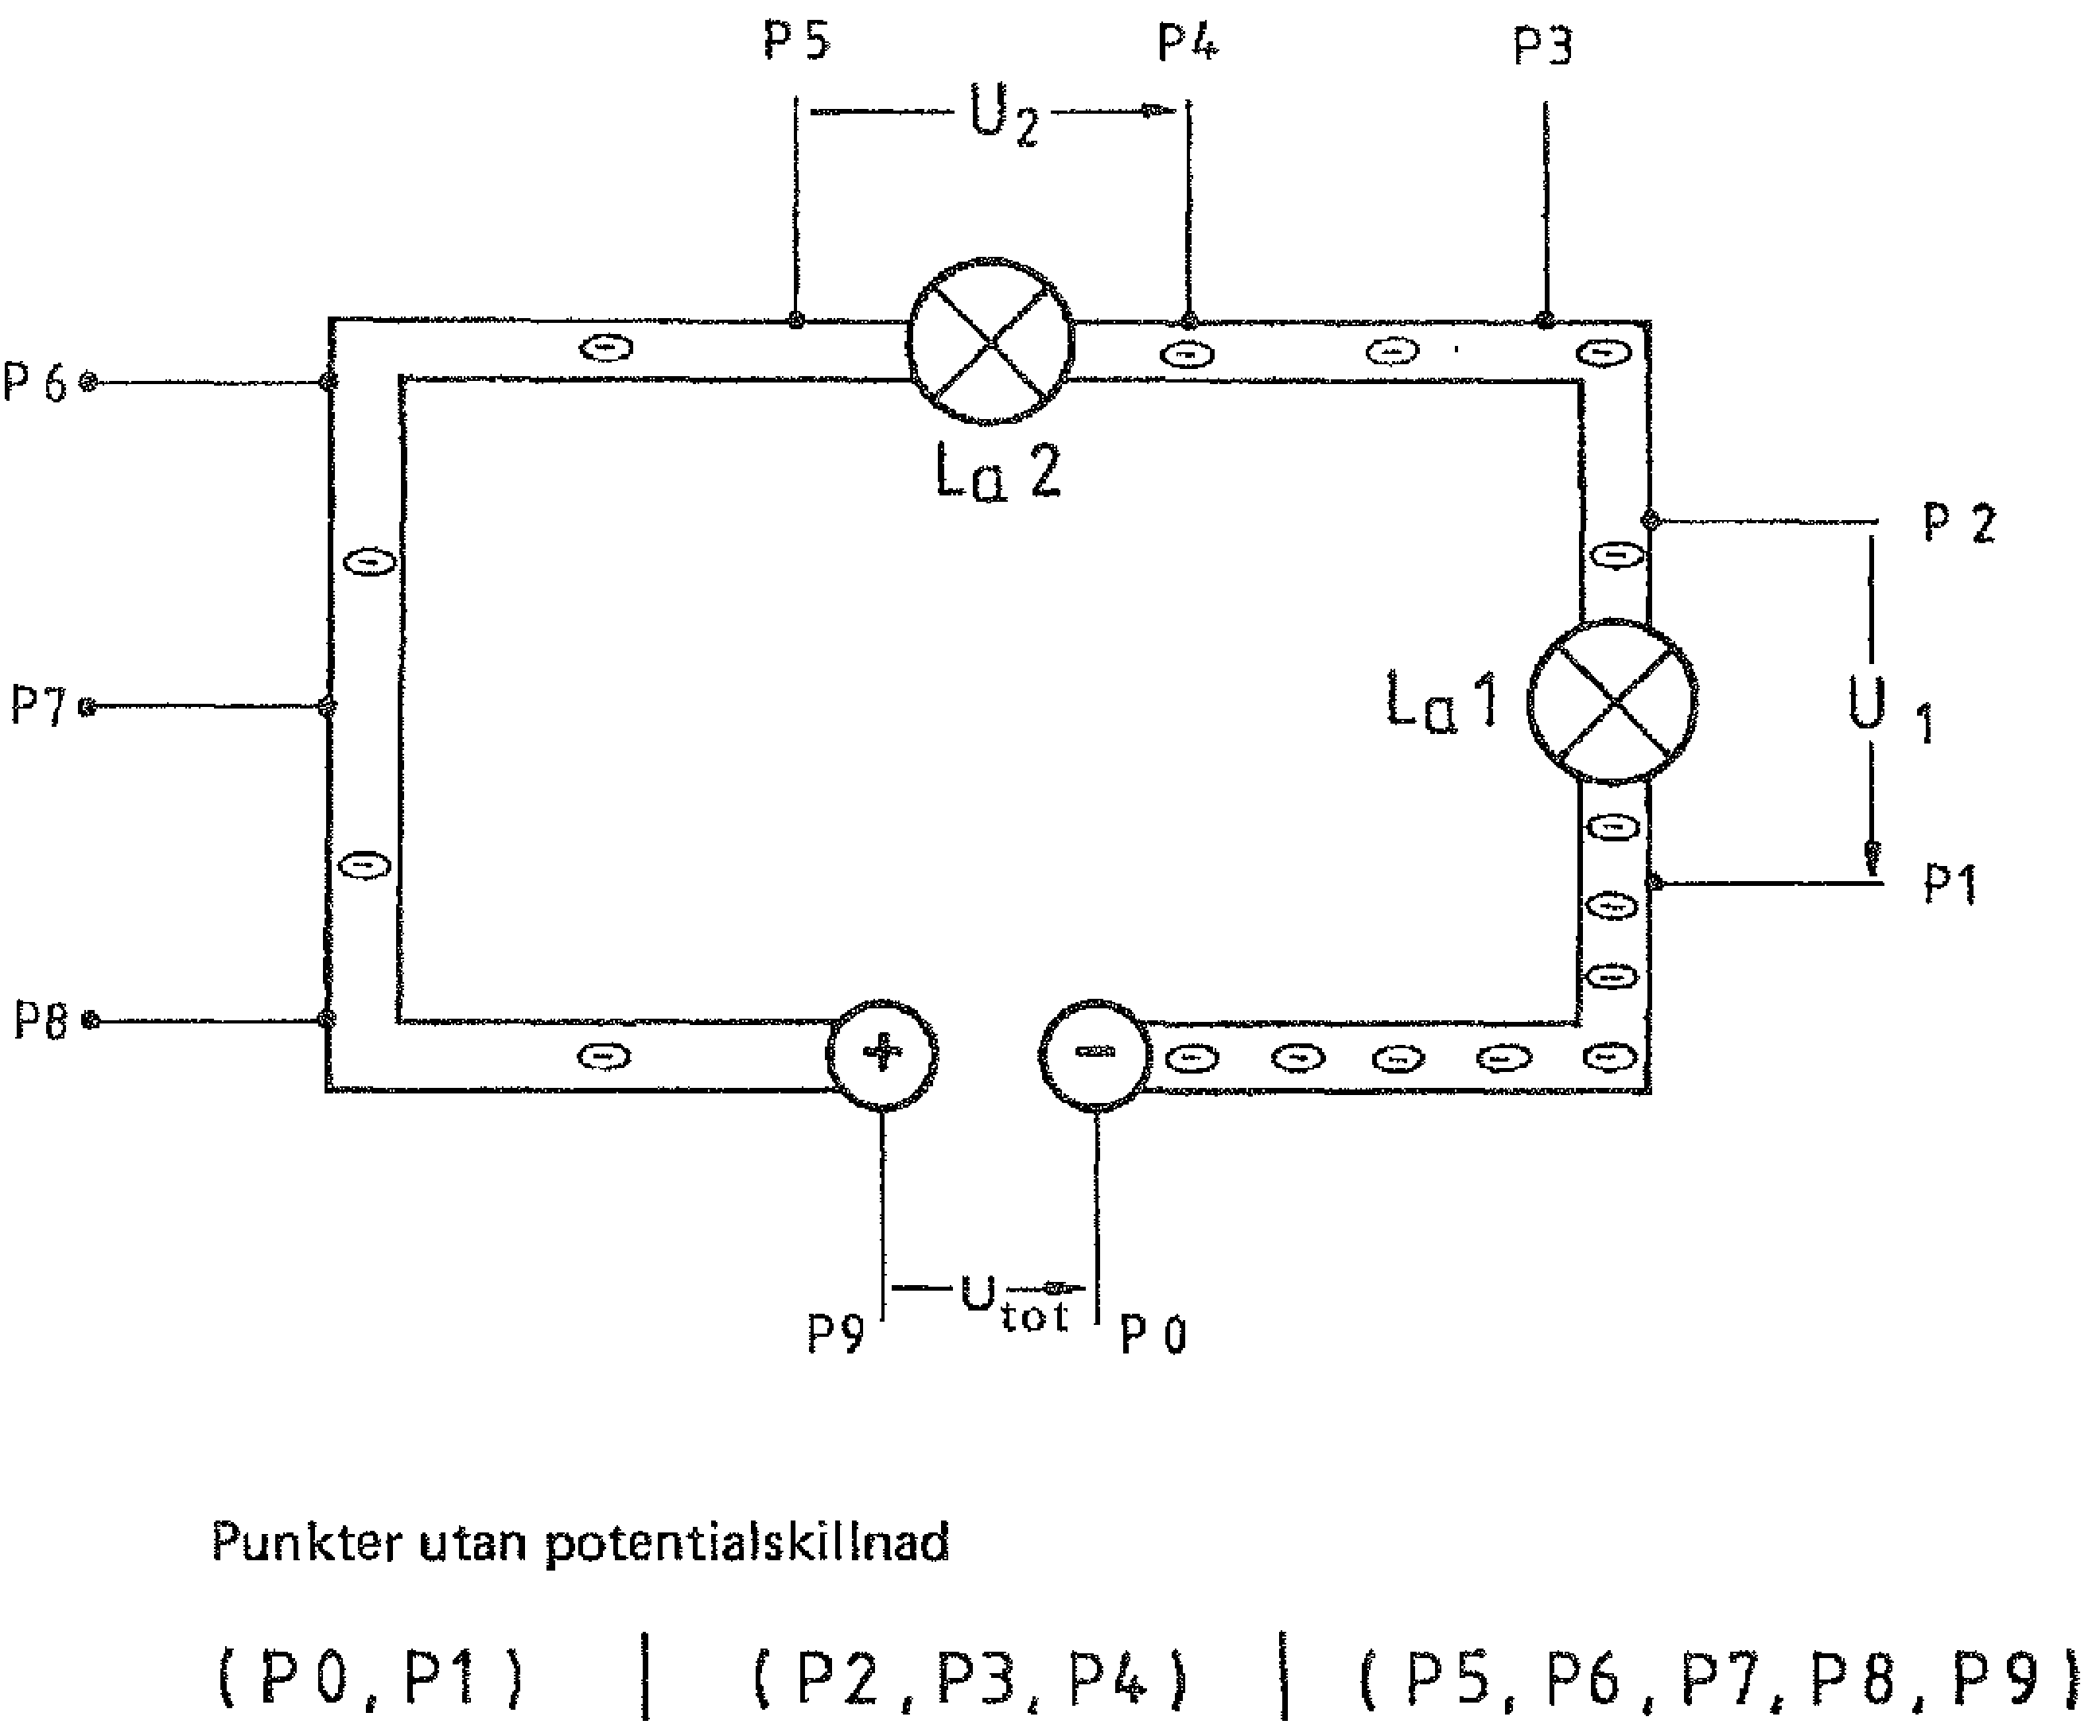
\includegraphics[width=0.6\textwidth]{images/cropped_pdfs/bild_2_1-03.pdf}
\caption{Potential och spänning i en strömkrets}
\label{fig:BildII1-3}
\end{center}
\end{figure*}

Bild \ref{fig:BildII1-3} visar potential och spänning i en strömkrets.

En elektrisk strömkrets består av en eller flera energikällor och
energiförbrukare.
Källor kan vara batterier, nätaggregat etc.
Förbrukare kan vara lampor, ledningar etc.
Varje energiförbrukare har en resistans och de elektriska laddningarna ''köar''
före förbrukaren, strax efter förbrukaren finns ingen kö.
Det uppstår en skillnad i laddningsmängd (en potentialskillnad) mellan varje
punkt i en strömkrets, när det flyter ström.
Man talar om spänningsfall.

\subsection{Strömförlopp}
\textbf{FÖRDJUPNING}
\index{strömförlopp}

Likströms- och växelströmsförloppen kan vara sammansatta av ett huvudförlopp och
underordnade förlopp.

Likström kan ha konstant styrka eller den kan variera enligt något förlopp, men
växlar aldrig riktning.

Växelström kan variera enligt något visst förlopp, t.ex. sinusvåg,
fyrkantsvåg, och växlar ständigt riktning.

\subsection{Resistans -- Enheten ohm}
\textbf{HAREC a.\ref{HAREC.a.1.1.2}\label{myHAREC.a.1.1.2c}, a.\ref{HAREC.a.1.1.3}\label{myHAREC.a.1.1.3c}}
\index{resistans}
\index{ohm (\(\Omega\))}
\index{enheter!ohm (\(\Omega\))}
\index{symbol!\(R\) resistans}

När fria elektroner tvingas fram genom atomstrukturen i en ledare, t.ex.
glödtråden i en lampa, så avgår energi i form av värme.
Detta fenomen kallas för resistans (av latinets resistere som betyder att
motstå).
Resistansen och därmed förlusterna i en strömkrets fördelas i
förhållande till de ingående materialen och deras dimensionering.

Resistans uttrycks i enheten \emph{ohm} \cite{SIbrochure8} och betecknas med
den grekiska bokstaven omega (\(\Omega\)).

I formler betecknas resistansen i en elektrisk krets eller en del av den med
\(R\).

Resistansen i en resistor är \(1\ [\Omega]\), när en spänning av \(1\ \mathrm{[V]}\)
driver en ström av \(1\ \mathrm{[A]}\) genom den resistorn.

\subsection{Ohms lag}
\textbf{HAREC a.\ref{HAREC.a.1.1.4}\label{myHAREC.a.1.1.4}}
\index{Ohms lag}
\index{resistor!Ohms lag}

Ohms lag beskriver sambandet mellan grundbegreppen ström
\(I\ \mathrm{[ampere]}\), spänning \(U\ \mathrm{[volt]}\) och resistans
\(R\ \mathrm{[ohm]}\).
Sambandet gäller både för likspänning och för effektivvärdet av växelspänning och
växelström.

I en ledare med resistansen \(R\) är strömstyrkan \(I\) genom resistansen
proportionell mot den pålagda spänningen \(U\).

\(
\begin{array}{lllll}U=I \cdot R & & I=\dfrac{U}{R} & & R=\dfrac{U}{I}\end{array}
\)

\subsection{Kirchhoffs lagar}
\textbf{HAREC a.\ref{HAREC.a.1.1.5}\label{myHAREC.a.1.1.5}}
\index{Kirchhoffs lagar}
\index{Kirchhoffs strömlag}
\index{Kirchhoffs spänningslag}

Den tyske fysikern G R Kirchhoff (1824--1887) formulerade sina välkända lagar
först 1845 och sedan 1847.

Kirchhoffs strömlag:

Den algebraiska summan av alla strömmar, som flyter till eller från varje punkt
i en elektrisk krets, är lika med noll.

\(I_1 + I_2 + I_3 + \cdots + I_n = 0\)

Kirchhoffs spänningslag:

I varje sluten strömkrets är den algebraiska summan av alla spänningskällor lika
med det totala spänningsfallet i alla resistorer.

Uttryckt på ett annat sätt är algebraiska summan av spänningarna i en
strömkrets lika med noll.

\subsection{Elektrisk effekt -- Enheten watt}
\textbf{HAREC a.\ref{HAREC.a.1.1.6}\label{myHAREC.a.1.1.6}, a.\ref{HAREC.a.1.1.7}\label{myHAREC.a.1.1.7}}
\index{elektrisk effekt}
\index{effekt}
\index{voltampere (VA)}
\index{enheter!voltampere (VA)}
\index{watt (W)}
\index{enheter!watt (W)}
\index{symbol!\(P\) effekt}

När en ström flyter genom en resistans utvecklas värme.
Värme är en form av effekt, som är högre ju starkare strömmen och högre
spänningen är.

Måttenheten \emph{voltampere} \(\mathrm{[VA]}\) för elektrisk effekt härleds ur
produkten av volt \(\mathrm{[V]}\) och ampere \(\mathrm{[A]}\).

För effekt som alstras av likström används enheten \emph{watt} \(\mathrm{[W]}\)
\cite{SIbrochure8} i stället för \emph{voltampere} \(\mathrm{[VA]}\).
Vid sidan om grundenheten \(1\ \mathrm{W}\) används delar och multipler av
denna.

\(1\ \mathrm{volt\ [U]}\ \cdot\ 1\ \mathrm{ampere\ [I]}\ =\ 1\ \mathrm{watt\ [P]}\)

Effektformeln \(P = U \cdot I\) gäller i första hand för likström men även för
växelström om belastningen är resistiv och ström och spänning inte är
fasförskjutna.
Formeln kan för att underlätta beräkningar skrivas om på flera sätt.

Vi börjar med att lösa ut \(I \quad \text{ur Ohms lag} \quad U = R \cdot I\) 

\(
I = \dfrac{U}{R}\\
\)

Vi sätter sedan in uttrycket för \(I\) i effektformeln

\(
\begin{array}{lllll}
P=U \cdot I & \Rightarrow & P= \dfrac{U \cdot U}{R} & \Rightarrow & P= \dfrac{U^2}{R}\\
\end{array}
\)

På motsvarande sätt kan vi ersätta \(U \quad\text{med}\quad R \cdot I\)

\(
\begin{array}{lllll}
P=U \cdot I & \Rightarrow & P = R \cdot I \cdot I  & \Rightarrow & P = R \cdot I^2\\
\end{array}
\)

Med hjälp av dessa formler kan effekten beräknas ur resistans- och strömvärdena
respektive ur resistans- och spänningsvärdena.
För övriga formler se formelsnurran bild \ref{fig:BildII1-4}

\subsection{Elektrisk arbete -- Enheten joule}
\textbf{FÖRDJUPNING}
\index{elektriskt arbete}
\index{joule (J)}
\index{enheter!joule (J)}
\index{symbol!\(W\) energi, arbete}

Energi finns i olika former, alltid och överallt.
Energi kan varken skapas eller förstöras, bara omvandlas från en form till en
annan.
Formen kan vara mekanisk, kemisk, elektrisk etc.

Arbete är omvandlingsprocessen från en energiform till en annan.

Arbetsmängden i alla energiformer kan mätas med samma enhet \emph{joule}
\(\mathrm{[J]}\) \cite{SIbrochure8} och anges med symbolen \(W\) för Work.

\(1\ \mathrm{joule}\) motsvarar det arbete som utvecklas när ett föremål
förflyttas \(1\ \mathrm{meter}\) med kraften \(1\ \mathrm{newton\ [N]}\),
d. v. s. \(1\ \mathrm{newtonmeter\ [Nm]}\).

\(W = l \cdot F \ \ \ \mathrm{[J] = [Nm]}\)

Arbetet \(W\ \mathrm{[J]}\) är mer ju längre tid \(t\ [s]\) en viss effekt
\(P\ \mathrm{[W]}\) utvecklas.

\(W = t \cdot P \ \ \ \mathrm{[J] = [sW]}\)
  
\subsection{Joules lag}
\textbf{HAREC a.\ref{HAREC.a.1.1.8}\label{myHAREC.a.1.1.8}}
\index{Joules lag}

\(Arbete\ =\ Effekt\ \cdot\ tid\ \ \ \mathrm{[W]} = \mathrm{[P]} \cdot \mathrm{[s]}\)

Eftersom effekten uttrycks som \(P = U \cdot I\) kan det elektriska arbetet
uttryckas som \(W = U \cdot I \cdot t\), vilket också är Joules lag.

Om grundenheterna för volt \(\mathrm{[U]}\), ampere \(\mathrm{[I]}\) och
sekund \(\mathrm{[s]}\) sätts in i formeln fås en måttenhet, uttryckt som
voltamperesekunder \(\mathrm{[VAs]}\) eller wattsekunder \(\mathrm{[Ws]}\)
eller joule\ \(\mathrm{[J]}\).

Måttenheten för elektriskt arbete är \(1\ joule\ per\ sekund\), som vanligen
kallas \(1\ \mathrm{wattsekund}\ \mathrm{[1\ Ws]}\).
Vid sidan av grundenheten används multipler av denna.
Exempel:
\(
\begin{array}{llll}
1\ \mathrm{kilowattsekund} & = 1\ \mathrm{kWs} & = 1\ 000\ \mathrm{Ws} & = 1,0 \cdot 10^3\ \mathrm{Ws}\\
1\ \mathrm{wattimme} & = 1\ \mathrm{Wh} & = 3\ 600\ \mathrm{Ws} & = 3,6 \cdot 10^3\ \mathrm{Ws} \\
1\ \mathrm{kilowattimme} & = 1\ \mathrm{kWh} & = 1 000\ \mathrm{Wh} & = 3,6 \cdot 10^6\ \mathrm{Ws}
\end{array}
\)

\subsection{Formelsnurran}
\index{formelsnurran}
\textbf{FÖRDJUPNING}

\begin{figure*}[ht]
\begin{center}
  %%\begin{wrapfigure}{R}{0.3\textwidth}
  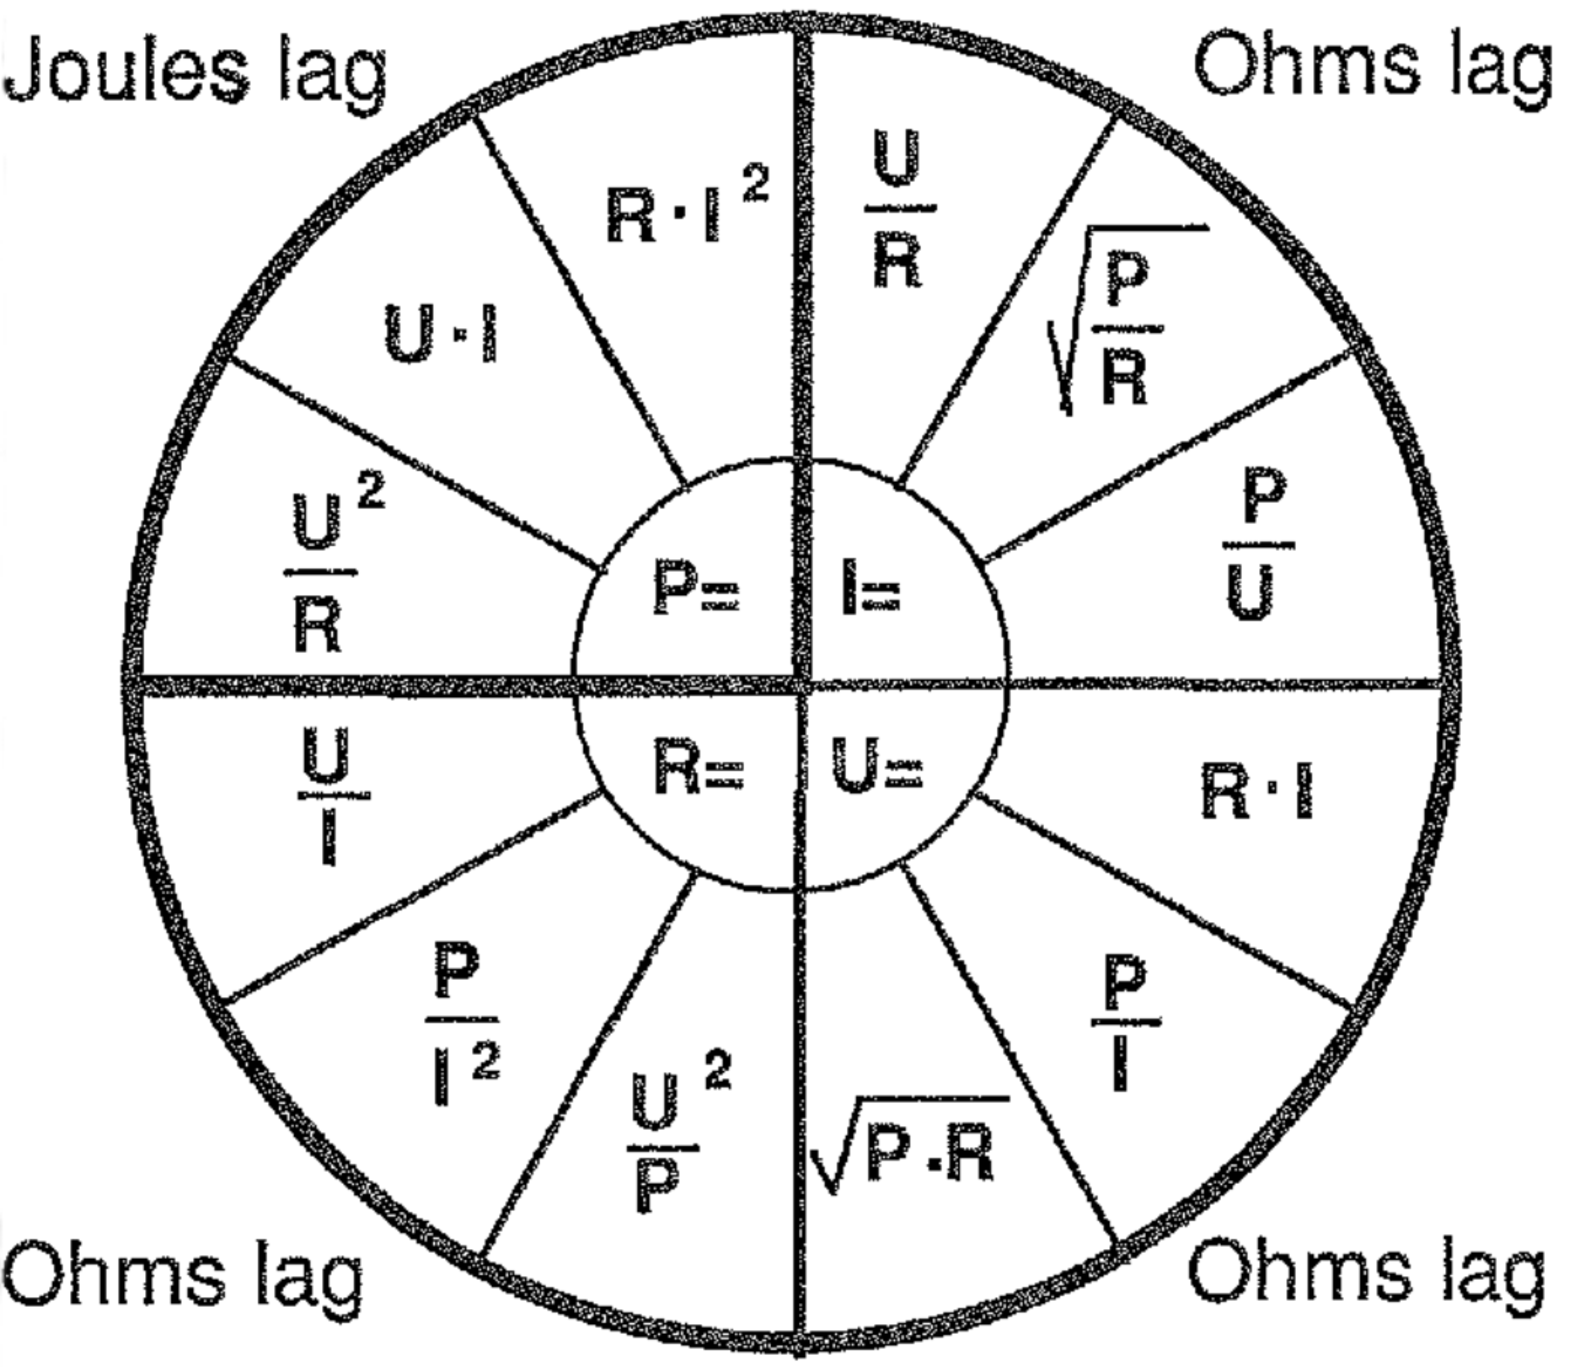
\includegraphics[width=0.5\textwidth]{images/cropped_pdfs/bild_2_1-04.pdf}
  \caption{''Formelsnurra'' för Ohms och Joules lagar}
  \label{fig:BildII1-4}
  %  \vspace{-100pt}
  %%\end{wrapfigure}
\end{center}
\end{figure*}

Så här finner man rätt formel i ''snurran'' (bild \ref{fig:BildII1-4}):
Välj ett segment med önskad storhet \(I\), \(U\), \(R\) eller \(P\) som det
första ledet i formeln.
Inom valt segment finns tre alternativ för det andra ledet i formeln.
Välj det alternativ som innehåller två kända storheter.

Bild \ref{fig:BildII1-4} visar ''Formelsnurra'' för Ohms och Joules lagar.

Exempel:

\subsubsection{Ohms lag}

\(R\) söks, \(U\) och \(I\) är kända;
Om \(U = 230\ V\) och \(I = 2\ A\), så blir

\(R=\dfrac{U}{I}=\dfrac{230}{2}=115\ \Omega\)

\subsubsection{Joules lag}

\(P\) söks, \(U\) och \(I\) är kända;

Om \(U = 230\ V\) och \(I = 2\ A\), så blir

\(P = U \cdot I = 230 \cdot 2 = 460\ W\)

\subsection{Amperetimmar (Ah) och batterikapacitet}
\textbf{HAREC a.\ref{HAREC.a.1.1.9}\label{myHAREC.a.1.1.9}}
\index{amperetimmar (Ah)}
\index{batterikapacitet}
\index{batteri}
\index{ackumulator}
\index{polspänning}
\index{elektrisk cell}

Det finns flera sätt att lagra energi.
Ett sätt är att göra det i kemisk form i speciella celler, där man kan ta ut
energin i elektrisk form.

Det finns celler som kan laddas upp och laddas ur upprepade gånger, s.k.
ackumulatorer.
Det finns också sådana celler som endast kan användas en gång och som inte
kan laddas upp igen, s.k. primärceller.

Energi i form av en elektrisk laddning kan även lagras i en kondensator.
Energin kan då lagras och tas ut utan omvandling.

Kapaciteten i en elektrisk cell uttrycks som produkten av den ström
\(\mathrm{[A]}\) som cellen avger och under den tid \(\mathrm{[s, h]}\) detta
kan ske.
Uttryckt med tidsenheten timmar blir då kapaciteten \(\mathrm{[Ah]}\).

Den kapacitet som anges i en cells produktdata är den nominella.
Denna kapacitet gäller endast under vissa normerade förhållanden såsom
celltemperatur, strömstyrka och urladdningstid.

Den praktiska kapaciteten i en cell begränsas av användningen.
En elektrisk cell avger sålunda regelmässigt mindre energimängd, ju högre
urladdningsströmmen är.
Kapaciteten i en elektrisk cell skiljer sig i det avseendet från den i
t.ex. en oljetank, där man kan ta ut lika mycket energimängd som man häller i
och oberoende av hur fort man gör det.

Elektriska celler kan samlas till s.k. batterier, varvid cellerna oftast
seriekopplas.
Batteriets polspänning är då summan av cellernas polspänningar.

Hur stort arbete ett batteri avger, beror såväl på hela batteriets
polspänning som på de enskilda cellernas kapacitet.
Exempel:
Ett batteri med polspänningen \(12\ \mathrm{V}\) och cellkapaciteten
\(100\ \mathrm{Ah}\) kan nominellt avge
\(P = U \cdot I = 12 \cdot 100 = 1200\ \mathrm{VAh} = 1,2\ \mathrm{kWh}\).

Hur länge batteriet ''räcker'' per laddning beror som sagt bl.a. på vilken
strömstyrka man tar ut.
Tar man ut \(1\ \mathrm{A}\) ur \(100\ \mathrm{Ah}\)-cellen här ovan, så blir
urladdningstiden nominellt
\(t = 100\ \mathrm{Ah}/1\ \mathrm{A} = 100\ \mathrm{h}\).

%\cleardoublepage
%\section{Elektriska kraftkällor}
\textbf{HAREC a.\ref{HAREC.a.1.2}\label{myHAREC.a.1.2}}

\subsection{Elektromotorisk kraft - EMK}

Det som driver ström genom en elektrisk strömkrets är kretsens elektromotoriska
kraft (EMK).

\begin{quote}
\emph{Måttenheten för EMK är \(Volt\ [V]\).}

\emph{EMK är summan av de potentialökningar som uppstår i kretsen.}
\end{quote}

De vanligaste slagen av emk är
\begin{itemize}
\item elektromagnetisk emk som uppkommer i strömledare i magnetfält som
varierar (ex. lindningarna i en roterande generator),
\item elektrokemisk emk som uppkommer i beröringsytan mellan en metallisk
ledare och en elektrolyt (ex. battericell),
\item elektrostatisk emk, t. ex. i kondensatorer,
\item kontaktemk i beröringsytan mellan metaller med olika termoelektrisk
potential eller mellan metall och luftens syre (ex. korrosion mellan metaller),
\item termoemk som uppkommer i en strömkrets där två sammanlödda metaller med
olika temperatur ingår (ex. termokors för strömmätning).
\end{itemize}

\subsection{Polspänning}

\begin{quote}\emph{
Den spänning, som kan mätas mellan kretsens anslutningspoler då kretsen är öppen.
}\end{quote}

\subsection{Inre resistans}

Liksom att komponenterna i strömkretsen har en viss resistans, så har också en
strömkälla en inre resistans. Den inre resistansen i en strömkälla ingår i
kretsens totala resistans.

\subsection{Kortslutningsström}

Om man på kortaste väg förbinder strömkällans anslutningspoler så blir kretsen
totala resistans lika med källans inre resistans.

Den kortslutningsström som då uppstår, begränsas enbart av strömkällans
polspänning och inre resistans.

Eftersom den inre resistansen oftast är mycket liten blir kortslutningsströmmen
motsvarande hög.

\subsection{Serie- och parallellkopplade kraftkällor}

\subsubsection{Seriekopplade kraftkällor}

För att uppnå en högre total spänning (emk) kan flera kraftkällor
(delspänningar) kopplas i en slinga efter varandra. Detta kallas seriekoppling.

\begin{quote}
\emph{Seriekopplade delspänningarverkar med eller mot varandra, beroende på
deras inbördes polariteter.}

\emph{Den totala spänningen över kopplingen är summan av de ingående
de/spänningarna, med hänsyn taget till deras polariteter.}
\end{quote}

\subsubsection{Parallellkopplade kraftkällor}

För att erhålla högre ström, kan flera svagare kraftkällor parallellkopplas. Vid
parallellkoppling erhålls däremot inte högre spänning.

\begin{quote}
\emph{Vid parallellkoppling av kraftkällor \textbf{måste} deras polaritet vara lika.}
\end{quote}

För minsta utjämningsström mellan parallellkopplade kraftkällor bör även deras
polspänning och inre resistans vara så lika
som möjligt.

%\cleardoublepage
%\section{Elektriskt fält}
\textbf{HAREC a.\ref{HAREC.a.1.3}\label{myHAREC.a.1.3}}

\subsection{Potential}

Potentialskillnaden - spänningen - mellan olika laddade kroppar, skapar krafter
mellan varandra samt mellan dem och deras omgivning. Detta fenomen kallas
elektriskt kraftfält och är orsaken till att elektriskt laddade kroppar kan
komma i rörelse.

\subsection{Elektrisk laddning}

Elektriska laddningar är grunden för elektricitetsläran. Varje proton i
atomkärnan är bärare av en positiv laddning. Neutronerna i atomkärnan är
elektriskt neutrala. Antalet protoner i kärnan bestämmer därför ensamt kärnans
totala positiva laddning, kallat för kärnladdningstalet. Elektronerna som
kretsar omkring atomkärnan är bärare av var sin negativa laddning.

Elementarladdningen [ e ] är den laddning som finns i en elektron och har länge
ansetts vara den minsta möjliga laddningen. Nutida elektronfysik konstaterar
ännu mindre enheter, men detgår vi inte in på här.

Antalet protoner och elektroner i en atom är lika och elektronernas samlade
negativa laddning blir då lika stor som protonernas samlade positiva laddning.
När laddningar med olika polaritet är lika stora väger de ut varandra och blir
elektriskt neutrala till sin omgivning.

\begin{quote}\emph{
Måttenheten för elektrisk laddning är \(Coulomb\ [C]\).
}\end{quote}

Laddningsmängden \(1\ Coulomb\) motsvarar 6.25 trillioner (\(6.25\cdot10^{18}\))
elementarladdningar.

Sambandet mellan laddning och ström är

\(Q = I \cdot t\)

Laddning [Q] är ström [I] under tiden [t]

\(1 C= 1 A ·1 s= 1 amperesekund [1 As]\)

\(1 Coulomb = 1 Ampere·1 sekund\)

\subsection{Kraftfält omkring elektriska laddningar}

\begin{figure*}
\begin{center}
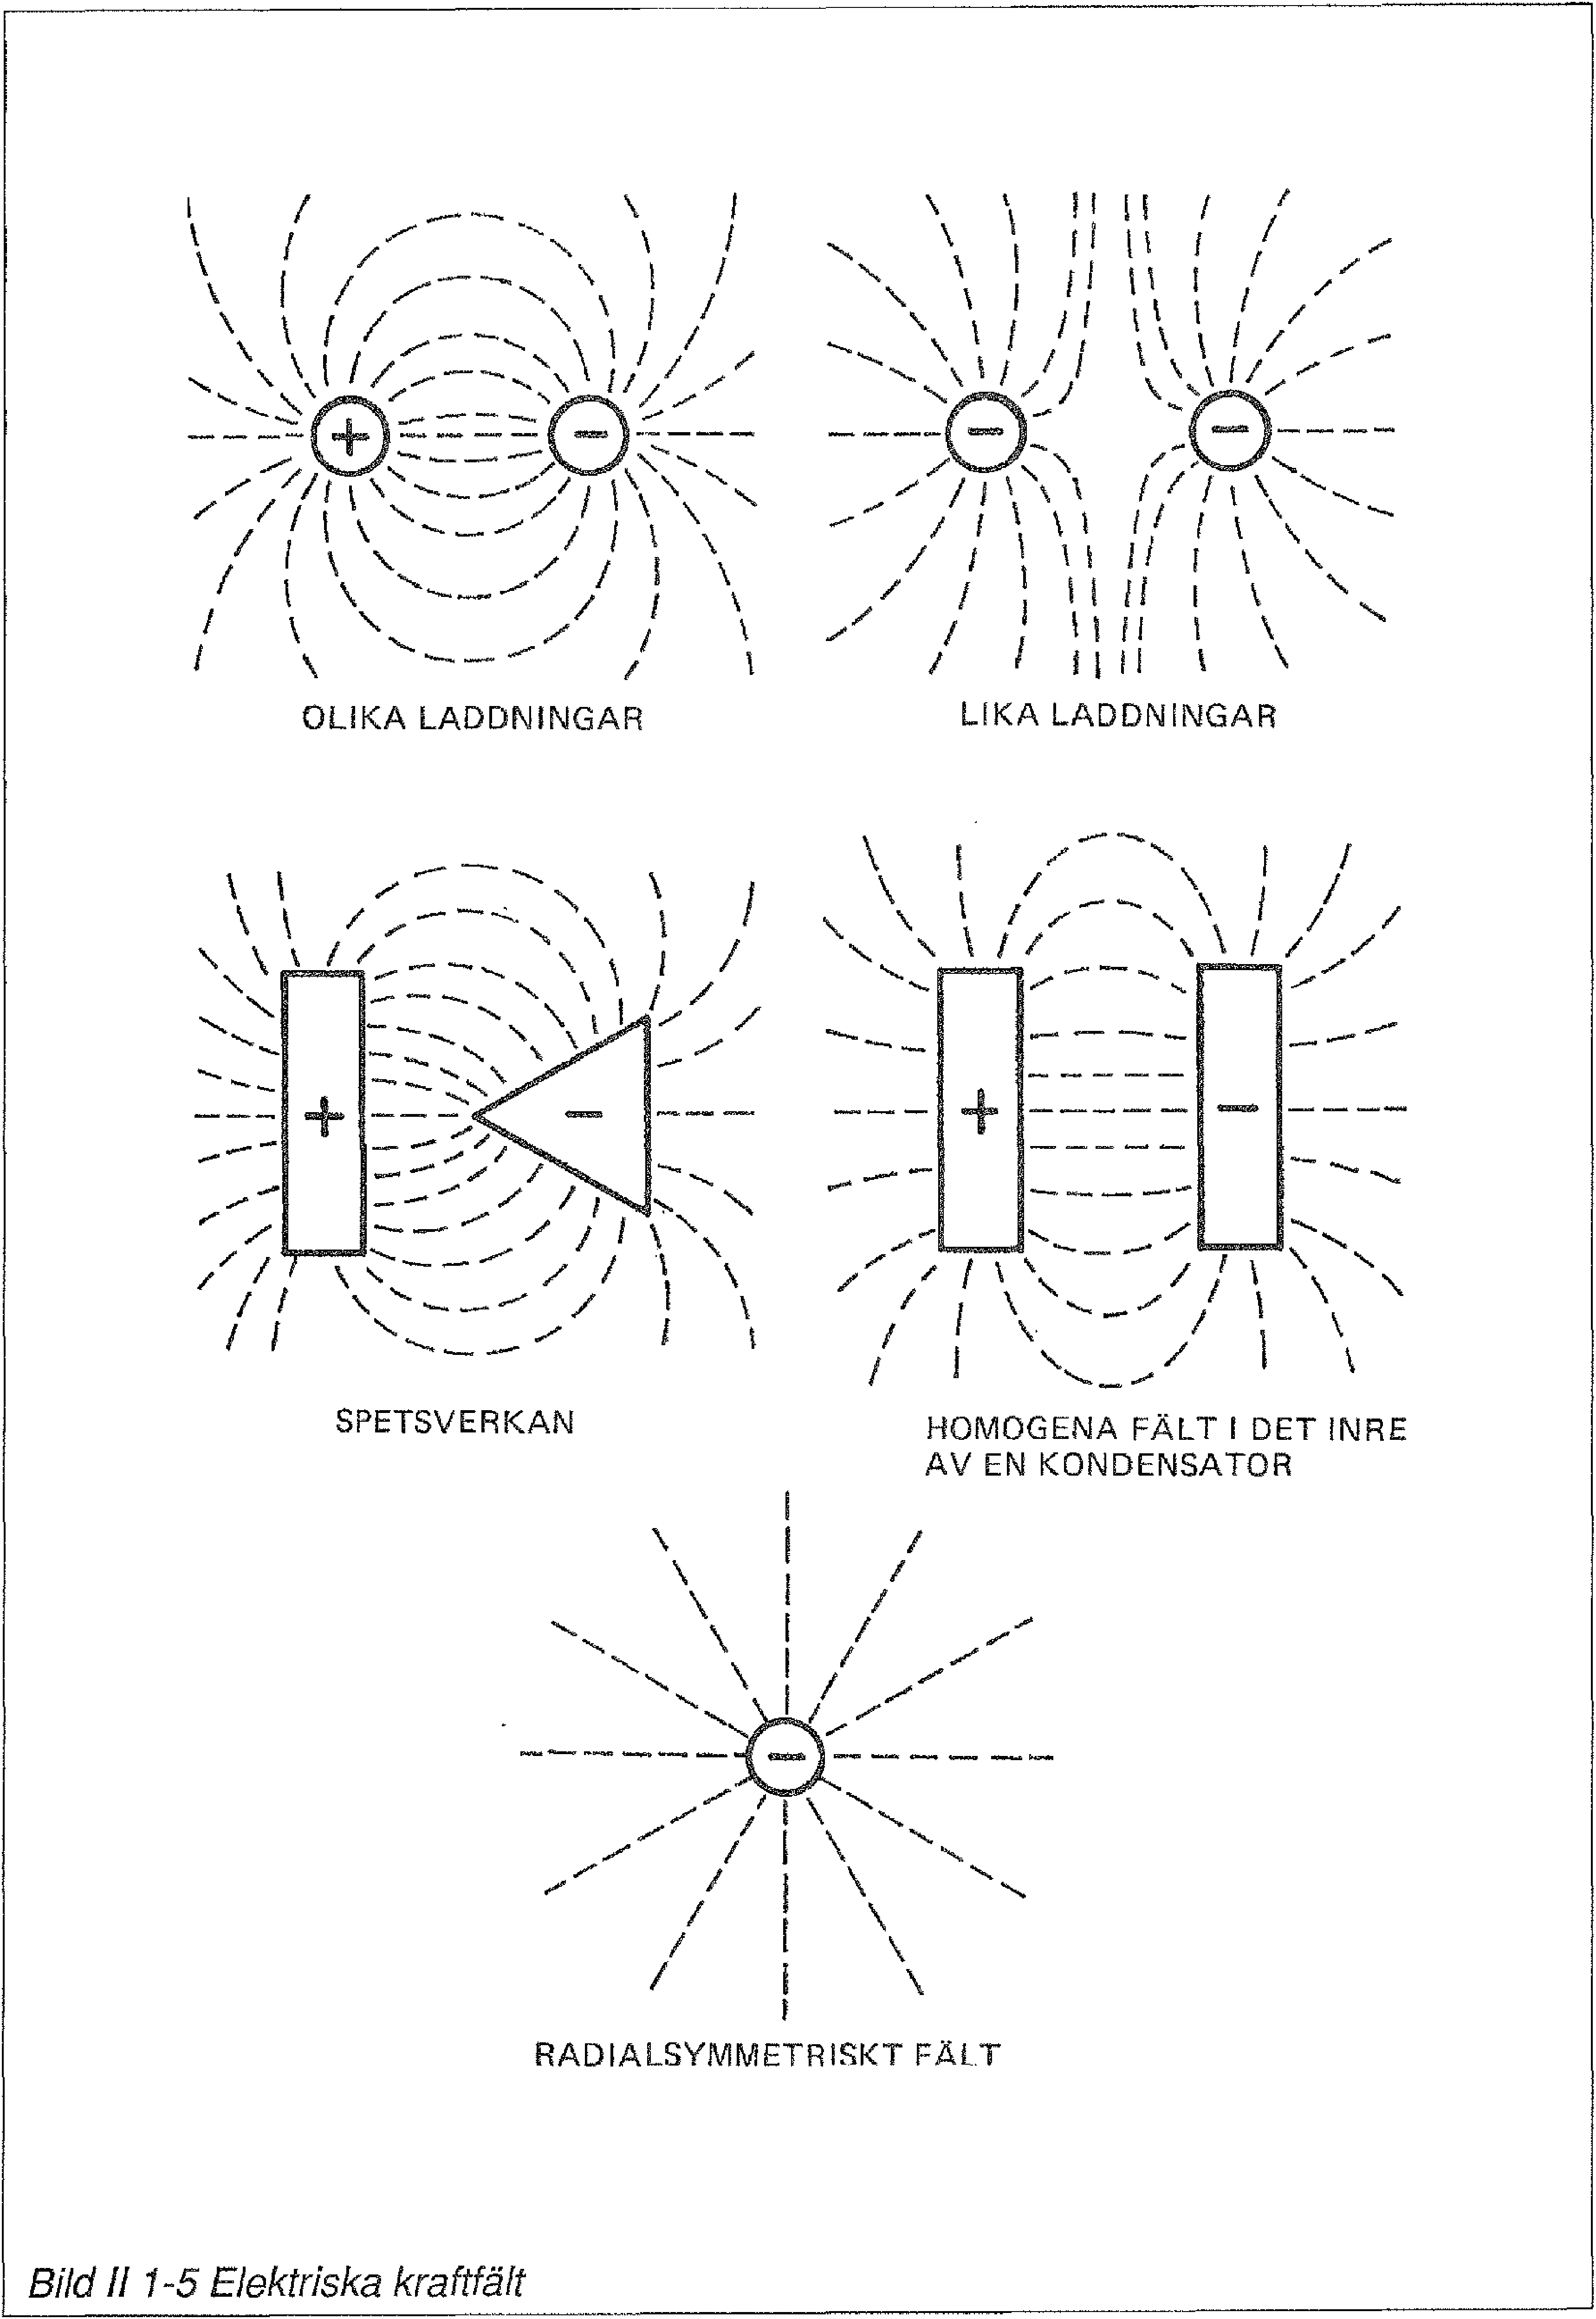
\includegraphics[width=14cm]{images/bild_2_1-05}
\caption{Elektriska kraftfält}
\label{fig:BildII1-5}
\end{center}
\end{figure*}

Fig. \ref{fig:BildII1-5}

Mellan elektriska laddningar bildas krafter.

\begin{itemize}
\item Varje laddning är omgiven av ett elektriskt kraftfält.
\item Mellan positiva (+) elektriska laddningar
och (-) negativa laddningar bildas krafter.
\item Fältkrafternas styrka och riktning symboliseras som linjer mellan positiva och
negativa laddningar, där styrkan är densamma utmed respektive linje.
\end{itemize}

(även 1.1)

\begin{quote}
\emph{Kroppar med olika slags laddningar dras till varandra}

\emph{Kroppar med lika slags laddningar stöter bort varandra}

\emph{Oladdade kroppar påverkas inte och ger ingen kraftverkan.}
\end{quote}

\subsection{Elektrisk fältstyrka}

I en trådformad ledare, som det flyter likström igenom, fördelas strömmen lika
över tvärsnittet. Om ledaren i stället är ett tunt plan, så blir
strömfördelningen annorlunda. Bilden visar ett plan med två elektroder, som
anslutits till en spänningskälla. Utmed sträckan mellan elektroderna fördelas
strömmen över planet så som strömlinjerna på bilden. Fördelningen beror på
elektrodernas utformning och polaritet. Strömtätheten är inte lika över hela
planet, eftersom planet kan ses som många parallellkopplade resistorer vars
resistanser ökar med tilltagande strömlinjelängd.

Strömtätheten i planet är större där resistansen mellan elektroderna är liten.
Närmast elektroderna där alla strömlinjer samlas är strömtätheten extremt hög.
Där strömtätheten är som störst finns den största potentialskillnaden
(spänningen) per längdenhet strömlinje. Man kan mäta potentialerna i planet.
Spänningen mellan två punkter utmed en tänkt strömlinje är därvid proportionell
med linjens längd mellan punkterna. Halva spänningen finner man mitt emellan
punkterna.

Elektriska fält är upplagrad energi. Fältstyrkan kan bli så hög, att det blir
en urladdning mellan polerna. Korona från ändarna av en antenn är ett annat
tecken på hög fältstyrka. För att försvåra urladdning kan man öka elektrodytan,
t.ex. göra den klotformad. Omvänt kan man medverka till urladdning genom att
minska elektrodytan. Ett exempel är åskledarens spets.


\begin{figure}
\begin{center}
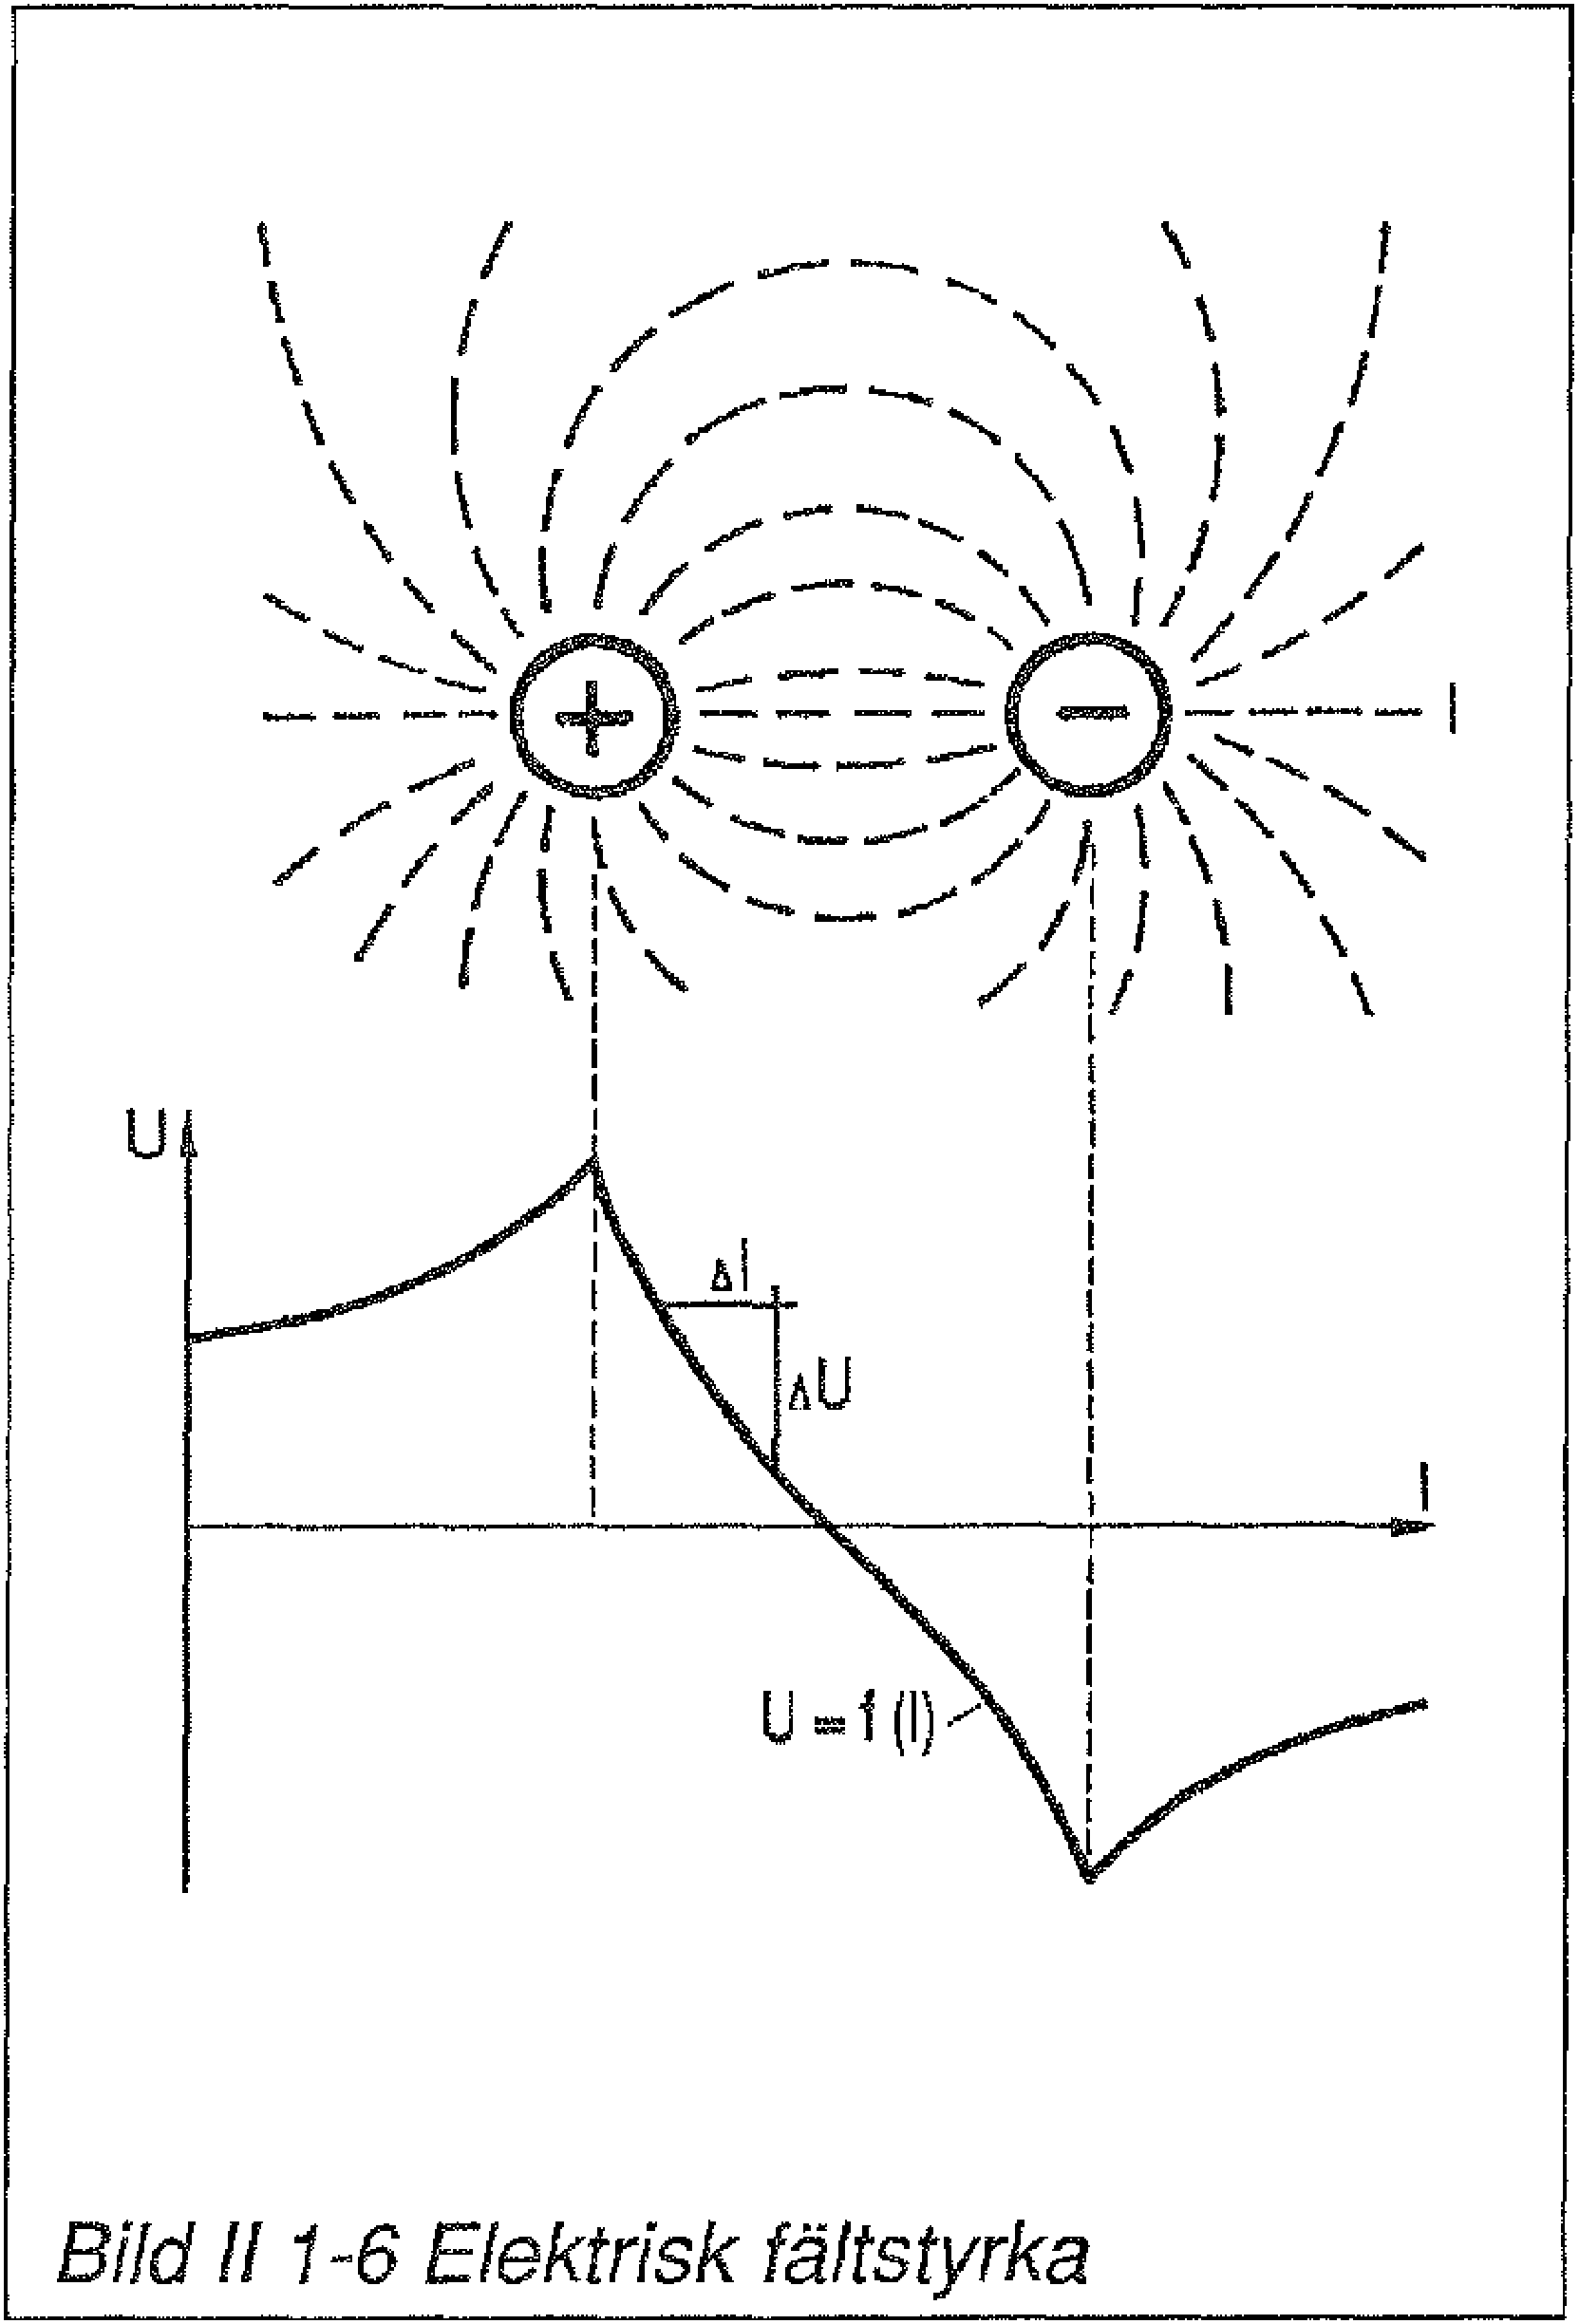
\includegraphics[width=7cm]{images/bild_2_1-06}
\caption{Elektrisk fältstyrka}
\label{fig:BildII1-6}
\end{center}
\end{figure}

Fig. \ref{fig:BildII1-6}

I diagrammet \(U = f(l)\) visas spänningarna utmed "mittströmslinjen" I genom
plus- och minuspolerna. Kurvutseendet är typisk även för omkring liggande
linjer, oavsett längd.

Bilden framställer en ledare som ett idealt plan, medan den i praktiken är en
volym. För att efterlikna en volym föreställer vi oss att bilden roterar
omkring mittströmslinjen, med fältlinjerna oförändrade. Även om resistansen i
den rotationskropp som uppstår är så hög att ingen ström flyter, så är
spänningsbilden fortfarande densamma.

Spänningsbilden gäller även för isolerande fasta material, gaser och vakuum.
Det finns alltså spänning mellan olika punkter även i "friska luften". Denna
spänningfältstyrka- kan mätas med särskilda instrument, s. k. fältstyrkemätare.

Av brantheten på spänningskurvan i bilden framgår vilken delspänningen är per
dellängd av en spänningslinje. Kvoten av delspänning och avståndet mellan
mätpunkterna kallar man för elektrisk fältstyrka.

\begin{quote}
\emph{I formler betecknas elektrisk fältstyrka med bokstaven \(E\).}
\emph{Elektrisk fältstyrka mäts i volt per meter.}
\end{quote}

\(
\begin{array}{cc}
E=\frac{\Delta U}{\Delta l} & \frac{[volt]}{[meter]}
\end{array}
\)

\subsection{Skärmning av elektriska fält}

I grunden finns det två slags fält, det elektriska och det magnetiska. Dessutom
finns det även elektromagnetiska fält, som är sammansatt av båda dessa. Fält
kan vara statiska eller dynamiska, varav här avses dynamiska. Ett dynamiskt
elektriskt fält genererar ett magnetiskt fält. Omvänt generar ett dynamiskt
magnetiskt fält ett dynamiskt elektriskt fält. Denna växelverkan gör att fälten
kan hållas igång av varandra med tillskott av yttre energi.

Fält i rörelse alstrar elektromagnetisk strålning, som påverkar omgivningen. När
påverkan inte är önskvärd måste fältet skärmas av. Ett sätt att skärma av ett
elektriskt fält är en metallisk kapsling som anslutits till apparatens
jordreferens. Skärmen behöver inte vara tät, men utförd så att all magnetiskt
inducerad ström i den bryts. (Jfr 1.4)

%\cleardoublepage
%\section{Magnetiskt fält}
\harec{a}{1.4}{1.4}
\label{elektromagnetiskafält}
\index{elektromagnetiska fält}

\subsection{Magnetism}
\index{magnetism}
\index{Plinius}
\index{Magnes}
\index{Lithos herakleia}
\index{Herakleia}
\index{Magnesia}
\index{Magnetes}

\infobox{
Enligt den romerske författaren \emph{Plinius} lär, vid tiden ungefär
160~år f.Kr. herden \emph{Magnes} en dag ha känt hur järnstiften i
sandalerna häftade vid en viss sorts sten.
Det kunde ha varit svart järnmalm, som grekerna i äldsta tider benämnde
\emph{Lithos herakleia} efter staden \emph{Herakleia} i Lydien,
där sådan malm förekommer.
Staden fick sedermera namnet \emph{Magnesia} och man kan tänka sig att stenen
kom att kallas \emph{Magnetes}.
En hel mineralgrupp med liknande egenskaper, såsom järn, nickel m.fl. kallas
magnetiska.
}

\emph{Magnetism} uppstår av elektriska laddningar i rörelse.
Elektronernas rörelser i en atom skapar nämligen magnetfält.
Det gör att atomerna var för sig fungerar som en magnetisk dipol -- en magnet.
I de flesta material är atomerna orienterade så att deras magnetiska krafter
tar ut varandra.
Materialet som helhet är då omagnetiskt och utövar inga yttre krafter.
Men vid påverkan från ett yttre magnetfält kan dipolerna (atomerna) i ett
material orienteras i samma riktning och deras magnetfält kommer då att
samverka. Hela materialet blir då magnetiskt.
När det yttre magnetfältet avlägsnas, kvarstår orienteringen endast delvis --
\emph{magnetisk remanens}.
I ferromagnetiska legeringar kvarstår en större del av orienteringen, även om
påverkan från det yttre magnetfältet har upphört.
Materialet är då permanentmagnetiskt.

\subsection{Kraftfält i och omkring magneter}

\end{multicols}
\mediumfig{images/cropped_pdfs/bild_2_1-07.pdf}{Kraftfält omkring magneter}{fig:BildII1-7}
\begin{multicols}{2}

Bild \ref{fig:BildII1-7} visar kraftfält omkring magneter.
Varje magnet omges av ett magnetiskt kraftfält.
Magnetfältets fördelning, styrka och riktningar beskrivs som kraftlinjer med
slutna kretslopp.

Utanför magneten går kraftlinjerna från nord- till sydpol och inne i magneten
motsatt riktning.
Kraftriktningen i varje punkt av fältet är den som nordändan på en kompassnål
skulle peka åt.
Om man hänger upp en magnet i en tråd, så kommer den att inta samma riktning
som jordens magnetfält.

\begin{quote}
\emph{Poler med samma polaritet stöter bort varandra (repellerar).}

\emph{Poler med olika polaritet dras till varandra (attraherar).}
\end{quote}

\mediumfig[0.5]{images/cropped_pdfs/bild_2_1-08.pdf}{Magnetiska fält omkring strömledare}{fig:BildII1-8}

\subsection{Magnetiska fält omkring strömbanor}
\harec{a}{1.4.1}{1.4.1}

Bild \ref{fig:BildII1-8} visar magnetiska fält omkring strömledare.
Omkring varje ledare, som det flyter en elektrisk ström igenom, alstras det ett
magnetiskt kraftfält.
Magnetiska kraftlinjerna fördelar sig koncentriskt omkring en rak ledare och
vinkelrätt mot denna.
Mellan ändarna av en ledare med bågformad utsträckning bildas kraftlinjer som
verkar med varandra.
En strömgenomfluten cylindrisk spole -- induktor -- uppvisar samma magnetiska
fältbild som en stavformad permanentmagnet.

\subsection{Bestämma magnetiska fältriktningen}

Magnetfältets riktning omkring en ledare kan enkelt bestämmas med
\emph{högerhandsregeln}.
När en \emph{ledare} fattas med höger hand och med tummen i strömmens
riktning, kommer fingrarna att peka i fältriktningen (B).

I bild \ref{fig:BildII1-8} (övre) så går strömmen från pluspolen (+) till
minuspolen (--) varvid strömmen kommer gå nedåt i bilden på ovansidan,
det vill säga precis så tummen pekar om man greppar ledaren med tummen nedåt,
och magnetfältet kommer att snurra som pilarna precis som de övriga fingrarna
på högerhanden.

När en ledare formas som en spole och en elektrisk ström flyter genom den,
kommer magnetfältet att ha ett utseende som liknar det omkring en
permanentmagnet.
En sådan spole kallas \emph{elektromagnet}.

Magnetfältets riktning i en spole kan också bestämmas med högerhandsregeln.
När \emph{en spole} fattas med höger hand och med fingrarna i strömmens
riktning, kommer den utsträckta tummen att peka mot spolens nordpol.

I bild \ref{fig:BildII1-8} (undre) så går strömmen från pluspolen (+) till
minuspolen (--) varvid strömmen kommer gå inåt i bilden på ovansidan, dvs.
precis så fingrarna pekar när man lägger handen på spolen, och magnetfältet
kommer att peka mot nord (N) precis som tummen på högerhanden.

Fälten omkring alla slags magneter, såväl permanentmagnetiska som
elektromagnetiska, återverkar på varandra.
Även enkla elektriska ledare är elektromagneter.

\subsection{Exempel på elektromagneter}

\tallfig{images/cropped_pdfs/bild_2_1-09.pdf}{Exempel på elektromagneter}{fig:BildII1-9}

Bild \ref{fig:BildII1-9} visar exempel på elektromagneter.

\subsubsection{Elektromagnet}
Det bildas ett magnetfält genom en spole så länge som det flyter ström genom
den.
En järnkärna i spolen koncentrerar fältet på grund av den större magnetiska
ledningsförmågan.

Elektromagneter används för att sätta magnetiska material i rörelse eller hålla
fast dem.

\subsubsection{Elektrisk ringklocka}
Anordningen består av en elektromagnet och en järnplatta på en fjäder.
På plattan sitter en självbrytande kontakt samt en kläpp som kan slå på en
klocka.

Kontakten åstadkommer en växelvis brytning och slutning av strömmen genom
elektromagneten.
Armaturen med kläppen kommer då i svängning och slår på klockan.

\subsubsection{Telefon}
I en enkel telefon finns bland annat en mikrofon, ett batteri och en
hörtelefon.

Särskilt i äldre telefoner består mikrofonen av en kolkornskammare med ett
membran.
Tryckvariationer (ljud) får membranet att vibrera, varvid resistansen genom
kolkornen varierar i motsvarande grad.
Därmed varierar talströmmen genom mikrofonen.

Hörtelefonen består av en elektromagnet och ett membran av mjukjärn.
Variationer i talströmmen genom mikrofonen passerar även hörtelefonen och får dess
magnetfält att variera.
Hörtelefonens membran alstrar då trycksvariationer, det vill säga ljud.

\subsubsection{Elektromagnetiskt relä}
Reläet består av en elektromagnet, en järnplatta (ankare) på en fjäder och en
elektrisk kontakt.
Med en svag ström / låg spänning genom spolen i manöverkretsen kan man med
reläets arbetskontakt styra starkare ström / högre spänning i huvudkretsen.

\subsection{Magnetisk fältstyrka}
\index{magnetisk fältstyrka}
\index{symbol!\(H\) magnetisk fältstyrka}

Som magnetisk fältstyrka förstår man flödet per meter fältlinje, det vill säga

\begin{align*}
  &H = \frac{\Theta}{l} = \frac{I \cdot N}{l} \\
  &H\ [A/m] \\
  &I\ [A] \\
  &N\ \text{[varvtal]} \\
  &l\ \text{[fältlinjelängd]}
\end{align*}

\emph{Magnetisk fältstyrka uttrycks således som ampere per meter flödesväg.}

\subsection{Magnetisk flödestäthet}
\index{magnetisk flödestäthet}
\index{tesla (T)}
\index{enheter!tesla (T)}
\index{symbol!\(B\) magnetisk flödestäthet}
\index{permabilitet}
\index{symbol!\(\mu\) permabilitet}

\emph{Den magnetiska flödestätheten mäts i enheten tesla \([T]\) (förut gauss).}

Formeltecknet/symbol är \(B\).

Formeln är \(B = \mu \cdot H\)

Flödestäthet \(B\ [Vs/m^2]\) Fältstyrka \(H\ [A/m]\)

\(\mu\) är permabilitetstalet för materialet.
\(\mu_0\) är permeabilitetstalet (fältkonstanten) för den magnetiska
ledningsförmåga för vakuum.

För järn eller annat magnetiskt ledande material tillkommer permeabilitetstalet
\(\mu_r\).
Det anger hur många gånger bättre än luft etc., som materialet leder ett
magnetisk flöde.
Permabilitetstalet kan då skrivas
\(\mu = \mu_r\mu_0\).

Formeln är \(B = \mu_0 \cdot \mu_r \cdot H\)

\subsection{Magnetiskt flöde}
\index{magnetiskt flöde}
\index{symbol!\(\Phi\) magnetiskt flöde}

Det magnetiska flödet är produkten av flödestätheten \(B\) och tvärsnittsytan
\(A\) av flödesvägen, således

\(\Phi = B \cdot A\)

\(\Phi \text{[weber eller Vs]}\) \(B \text{[T eller tesla]}\) \(A [m^2]\)

\subsection{Skärmning av magnetiska fält}
\harec{a}{1.4.2}{1.4.2}
\index{magnetiska fält!skärmning}
\label{elektromagnetisk skärmning}

I grunden finns det två slags fält, det elektriska och det magnetiska. Det
finns även elektromagnetiska fält som är sammansatta av båda dessa.
Fält kan vara permanenta eller rörliga, varav här avses de rörliga.
Ett rörligt magnetiskt fält genererar ett elektriskt fält.
Omvänt generar ett rörligt elektriskt fält ett rörligt magnetiskt fält.
Denna växelverkan gör att fälten kan hållas igång med tillförsel av yttre
energi.

Fält i rörelse alstrar elektromagnetisk strålning, som påverkar funktioner i
omgivningen.
När påverkan inte är önskvärd, måste fältet skärmas av.
Ett sätt att skärma magnetiska fält är en metallisk kapsling.
Kapslingen ska vara tät och bilda en sluten magnetisk krets.
Kapslingen ska vara utförd i ett material som är en god ledare av magnetiskt
flöde.
(Jämför \ref{elektrostatik skärmning})

%\cleardoublepage
%\section{Elektromagnetiska vågor}

\smallfig{images/cropped_pdfs/bild_2_1-10.pdf}{Vågor längs en linje}{fig:BildII1-10}

\harec{a}{1.5}{1.5}
\index{elektromagnetiska fält}

\subsection{Vågutbredning}
\harec{a}{1.5.1}{1.5.1}
\index{vågutbredning}

En tillståndsändring i ett medium innebär att energi tillförs eller tas bort.
Om detta sker växelvis uppstår förlopp såsom pendling, svängning, vågbildning etc.
Eftersom naturen söker jämvikt, så breder förloppet ut sig genom mediet efter
någon modell.

Energi kan inta olika tillstånd. I en pendel växlar energin mellan lägesenergi
och rörelseenergi.
Vågor på en vätskeyta liksom fjädring i fasta material är exempel på detta.
Det kan även innebära trycksvängningar i gaser och så vidare.

I detta avsnitt behandlas elektromagnetiska fält.
Sådana uppstår av svängningar i elektriska och magnetiska fält.
För att förklara pendling och utbredning används här modeller.

\subsection{Utbredningsmodeller}

\subsubsection{Vågutbredning längs en linje}

\smallfig{images/cropped_pdfs/bild_2_1-11.pdf}{Vågutbredning på en yta}{fig:BildII1-11}

Bild \ref{fig:BildII1-10} visar vågor längs en linje.
När änden av en tråd sätts i pendling med en frekvens \(f\), så kommer till
sist hela tråden i svängning med den frekvensen.
Den pendling, som först skapades, vandrar längs tråden med
utbredningshastigheten \(v\).
Våglängden är \(\lambda\) (lambda), som är avståndet mellan två närliggande
punkter med samma svängningsläge och svängningsriktning.

\subsubsection{Vågutbredning på en yta}
\index{vågutbredningshastighet}
\index{symbol!\(v\) vågutbredningshastighet}

Bild \ref{fig:BildII1-11} visar vågutbredning på en yta.
När ett föremål släpps genom en vätskeyta, så bildas vågor som breder ut sig
som cirklar i varandra (koncentriska).

De punkter på vågen, som för ögonblicket har samma svängningsläge, och är lika
långt från energikällan, kallas för vågfront.

Sambandet mellan utbredningshastighet \(v\), våglängd \(\lambda\) och frekvens
\(f\) är:
%%
\[
\begin{array}{llll}
v = \lambda \cdot f & v \ [m/s] & \lambda \ [m] & f \ [Hz=1/s]
\end{array}
\]
%%
Exempel: När våglängden \(\lambda = 2\ m\) och antalet svängningar per sekund
\(f = 10\ Hz\), så breder vågen ut sig med hastigheten \(v = 20\ m/s\).

\smallfig{images/cropped_pdfs/bild_2_1-12.pdf}{Vågutbredning i rummet}{fig:BildII1-12}

\subsubsection{Vågutbredning i rummet}

Bild \ref{fig:BildII1-12} visar vågutbredning i rummet.

Ljud är energi i form av tryckvågor i luften.
När en mekanisk kropp sätts i svängning (stämgaffel, dricksglas etc), överförs
svängningarna till den omgivande luftmassan som börjar att svänga med.
I luftmassan bildas det omväxlande över- och undertryckszoner, som breder ut
sig åt alla håll.
De mekaniska svängningarna i ljudkällan omvandlas alltså till tryckvågor.

Det mänskliga örat uppfattar tryckvågor inom frekvensområdet ca
15-\SI{18000}{Hz} som ljud.
Dessa vågor kallas ljudvågor.
Utbredningshastigheten för ljudvågor är \(v = \text{ca } 340\ \text{m/s}\) vid
15~\degree C och normalt lufttryck.

\subsection{Elektromagnetiska fält}
\harec{a}{1.5.2}{1.5.2}
\index{elektromagnetiska fält}

Tabell \ref{tab:elektromagnetiskt_spektrum} visar elektromagnetiskt spektrum.
I detta avsnitt görs i huvudsak endast jämförelse mellan ljusvågor och
radiovågor, vilka båda är elektromagnetisk strålning.
Hur ett elektromagnetiskt fält frigörs från en ledare framgår av kapitel
\ref{vågutbredning}.

Elektromagnetiska fält är energi, som är sammansatt av mycket snabbt svängande
elektriska och magnetiska fält.
När elektrisk ström genom en ledare ändras i styrka bildas ett magnetfält
omkring ledaren.
Detta magnetfält alstrar en elektromotorisk kraft (EMK), som är motriktad den
som driver fram strömmen.
Magnetfältet motverkar således strömändringen.
På liknande sätt alstrar en ändring av magnetfältet omkring ledaren en EMK i
form av ett elektriskt fält.
Detta driver en motriktad ström och därmed ett motverkande magnetiskt fält.

Både det elektriska och det magnetiska fältet har således alstrats av ändringar
i det andra och existerar därför bara tillsammans.

De båda fälten kombineras till ett elektromagnetiskt fält, som har egenskapen
att kunna stråla (breda ut sig) i alla tre dimensioner.
Beroende på frekvensen har elektromagnetiska fält olika egenskaper och
användning, vilket framgår av bilden.

\begin{table}
\begin{center}
\begin{tabular}{|rl|rl|l|}
\hline
\multicolumn{2}{|c|}{\multirow{2}{*}{Frekvens}} & \multicolumn{2}{c|}{\multirow{2}{*}{Våglängd}} & \multicolumn{1}{c|}{Egenskaper/} \\
 & & & & \multicolumn{1}{c|}{användning} \\ \hline
300 & Hz  & 100 & mil & \\
  1 & kHz & 300 & km & ULF \\ \cline{5-5}
  3 & kHz & 100 & km & \\
 10 & kHz &  30 & km & VLF \\ \cline{5-5}
 30 & kHz &  10 & km & \\
100 & kHz &   3 & km & LF \\ \cline{5-5}
300 & kHz &   1 & km & \\
  1 & MHz & 300 & m & MF \\ \cline{5-5}
  3 & MHz & 100 & m & \\
 10 & MHz &  30 & m & HF \\ \cline{5-5}
 30 & MHz &  10 & m & \\
100 & MHz &   3 & m & VHF \\ \cline{5-5}
300 & MHz &   1 & m & \\
  1 & GHz & 300 & mm & UHF \\ \cline{5-5}
  3 & GHz & 100 & mm & \\
 10 & GHz &  30 & mm & SHF \\ \cline{5-5}
 30 & GHz &  10 & mm & \\
100 & GHz &   3 & mm & EHF\\ \cline{5-5}
300 & GHz &   1 & mm & \\\
  1 & THz & 300 & \(\mu\)m & Infrarött \\
  3 & THz & 100 & \(\mu\)m & ljus \\
 10 & THz &  30 & \(\mu\)m & (värme- \\
 30 & THz &  10 & \(\mu\)m & strålning) \\
100 & THz &   3 & \(\mu\)m & \\ \cline{5-5}
300 & THz &   1 & \(\mu\)m & Synligt ljus \\ \cline{5-5}
  1 & PHz & 300 & nm & \\
  3 & PHz & 100 & nm & Ultraviolett \\
 10 & PHz &  30 & nm & ljus \\ \cline{5-5}
 30 & PHz &  10 & nm & \\
100 & PHz &   3 & nm & Rönt-\\
300 & PHz &   1 & nm & gen-\\
  1 & EHz & 300 & pm & strålning\\ \cline{5-5}
  3 & EHz & 100 & pm & \\
 10 & EHz &  30 & pm & Gamma-\\
 30 & EHz &  10 & pm & strål-\\
100 & EHz &   3 & pm & ning\\
300 & EHz &   1 & pm & \\
\hline
\end{tabular}
\end{center}
\caption{Elektromagnetiskt spektrum}
\label{tab:elektromagnetiskt_spektrum}
\end{table}

\subsubsection{Ljusvågor}
\index{ljusvågor}
\index{ljushastighet}
\index{symbol!\(c\) ljushastighet i vakuum}
\index{symbol!\(\lambda\) våglängd}

Ögat uppfattar elektromagnetisk strålning bara inom ett visst frekvensområde
som ljus.
Ljusets utbredningshastighet beror av vilket material, som det passerar igenom.
I vakuum är hastigheten störst, \(c = 299\, 792\, 458\ m/s\)
(= ca \(3 \cdot 10^8\ m/s\)) \cite{SIbrochure8}.
I tätare ämnen är hastigheten lägre, till exempel i glas ca \(200\, 000\, 000\ m/s\).
Det för människan synliga ljuset har våglängder mellan \(7,7 \cdot 10^{-7}\)
och \(3,9 \cdot 10^{-7}\ m\), motsvarande 7,7 till 3,9 tiotusendels mm.

Sambandet mellan ljusets utbredningshastighet \(c\) i vakuum, frekvensen \(f\)
och våglängden \(\lambda\) är
%%
\[
\begin{array}{llll}
c = \lambda \cdot f & c \ [m/s] & \lambda \ [m] & f \ [Hz]
\end{array}
\]
%%
\subsubsection{Radiovågor}
\index{radiovågor}

Även radiovågor är elektromagnetisk strålning, men inom ett lägre
frekvensområde än det för ljus.
Men utbredningshastigheten för radiovågor genom olika material följer ändå
samma lagar som de för till exempel ljusets utbredning.

Radiovågor anses omfatta ett frekvensområde från ca 10~kHz
(\(\lambda = 30\ km\)) till 300~GHz (\(\lambda = 1\ mm\)).

Rundradio tilldelas frekvenser i intervallet 100~kHz till 1000~MHz.
Amatörradio tilldelas ett antal frekvensområden i intervallet 1,8~MHz till
250~GHz.

Att märka är att elektromagnetiska fält, som sagts ovan, förekommer så långt
ner i frekvens som ett fåtal kHz.
Detta ska självklart inte förväxlas med ljudtryck med samma frekvens.

\subsubsection{Egenskaper hos elektromagnetiska vågor}

Elektromagnetiska vågor med högre frekvens än radiovågor uppfattas som
värmestrålning, vågor med ännu högre frekvens som ljus etc., men fortfarande är
huvudegenskaperna samma.
Som exempel kan nämnas polariserade vågor.
Dessutom kan man finna motsvarigheten till sådana egenskaper såsom interferens
och överlagring även i andra vågtyper, till exempel i ljud.

\subsection{Vågpolarisation}
\harec{a}{1.5.3}{1.5.3}
\label{vågpolarisation}
\index{vågpolarisation}

\largefig{images/cropped_pdfs/bild_2_1-14.pdf}{Polarisation av elektromagnetiska vågor}{fig:BildII1-14}

Bild \ref{fig:BildII1-14} visar polarisation av elektromagnetiska vågor.

\subsubsection{Vågor längs en linje (tråd e.d.)}
En vågrörelse i ett plan kallas linjärt polariserad.
Om änden på en horisontell tråd sätts i rörelse uppåt-nedåt, uppstår på tråden
en linjärt polariserad vågrörelse i vertikalplanet -- vertikal polarisering.
Om tråden sätts i rörelse höger-vänster kommer dess svängning att vara
horisontellt polariserad.
Om tråden sätts i svängning i ett plan och detta plan ständigt vrider sig,
kommer även vågrörelsen utmed tråden att vrida sig.
En vågrörelse, vars polarisering vrider sig roterar -- kallas för cirkulärt
polariserad.
Vridning mot- respektive medurs kallas för vänster- respektive högervriden
polarisering.

\subsubsection{Elektromagnetiska vågor}

De magnetiska och elektriska fälten omkring en ledare är vinkelrätt orienterade
mot varandra.
Det elektromagnetiska fält som de bildar tillsammans bildar en vågfront som
är vinkelrätt orienterad mot dem.

Polariseringsriktningen för en elektromagnetisk våg definieras som den riktning
dess elektriska fält har:
\begin{itemize}
  \item vertikalt elektriskt fält -- vertikal polarisering
  \item horisontellt elektriskt fält -- horisontell polarisering.
\end{itemize}

\subsubsection{Ljusvågor}

Ljus är elektromagnetiska vågor.
När dagsljus, som för övrigt är opolariserat, belyser ett polariseringsfilter
passerar endast de vågkomposanter genom filtret, som har samma polarisering
som filtret.

När det polariserade ljuset därefter sänds mot ett efterföljande filter,
passerar ljuset genom filtret endast när det har samma polarisering som ljuset.
När de båda filtren är vridna 90\degree~i förhållande till varandra, passerar
inget ljus alls.

\subsubsection{Radiovågor}

Radiovågor är elektromagnetiska vågor inom det frekvensområde som lämpar sig
för radiokommunikation.

Beroende på sändarantennens utformning avger den vågor med en polarisation.
På samma sätt är en mottagarantenn mest mottaglig för vågor med en viss
polarisation.
Överföringsförlusterna blir lägst mellan antenner med samma polarisation.

I det högre frekvensområdet för radio (VHF, UHF, SHF) är polariseringsvridning
under överföringen min\-d\-re vanlig.
Genom att utforma antennerna med horisontell, vertikal eller cirkulär (höger-
alternativt vänstervriden) polarisation fås överföringsegenskaper för olika
syften.

Cirkulärt polariserade antenner ger lägst överföringsförluster när
polariseringsriktningen är lika i sän\-d\-ar- och mottagarantennen.

I det lägre frekvensområdet för radio (HF och lägre) utnyttjas oftast
rymdvågsutbredning.
Eftersom de utsända vågorna då reflekteras mot jonosfärskikt, uppstår
polariseringsvridningar som inte kan förutses.
Då är det en fördel att kunna växla mellan antenner med olika polarisation.

\subsection{Våginterferens}

Bild \ref{fig:BildII1-15} visar våginterferens.
När vågor från olika energikällor blandas med varandra (överlagras), kommer
de att antingen samverka eller motverka.
Beroende av det tidsmässiga läget mellan vågorna och deras amplituder blir
resultatet en förstärkning eller en försvagning.
Om har samma frekvens och lika stora, motriktade amplituder, så uppstår en
utsläckning, vilket kallas fädning (eng. \emph{fading}).

Denna vågmekanism är liknande i gaser (luft), vätskor, elektromagnetiska fält
etc.
Ett försök kan göras med en stämgaffel som man slår an och håller intill örat.
När man vrider stämgaffeln runt sin längdaxel, kommer avståndet mellan
vart och ett av gaffelbenen och örat att variera.
Då uppstår en växelvis med- och motverkan mellan tonerna från gaffelbenen och
därmed varierande tonstyrka.

Detta fenomen utnyttjas bland annat i antenner för riktad sändning respektive
mottagning av radiovågor.

\mediumfig{images/cropped_pdfs/bild_2_1-15.pdf}{Våginterferens}{fig:BildII1-15}

%\cleardoublepage
%\section{Sinusformade signaler}
\textbf{HAREC a.\ref{HAREC.a.1.6}\label{myHAREC.a.1.6}}
\textbf{HAREC a.\ref{HAREC.a.1.6.1}\label{myHAREC.a.1.6.1}}

\begin{figure}[ht]
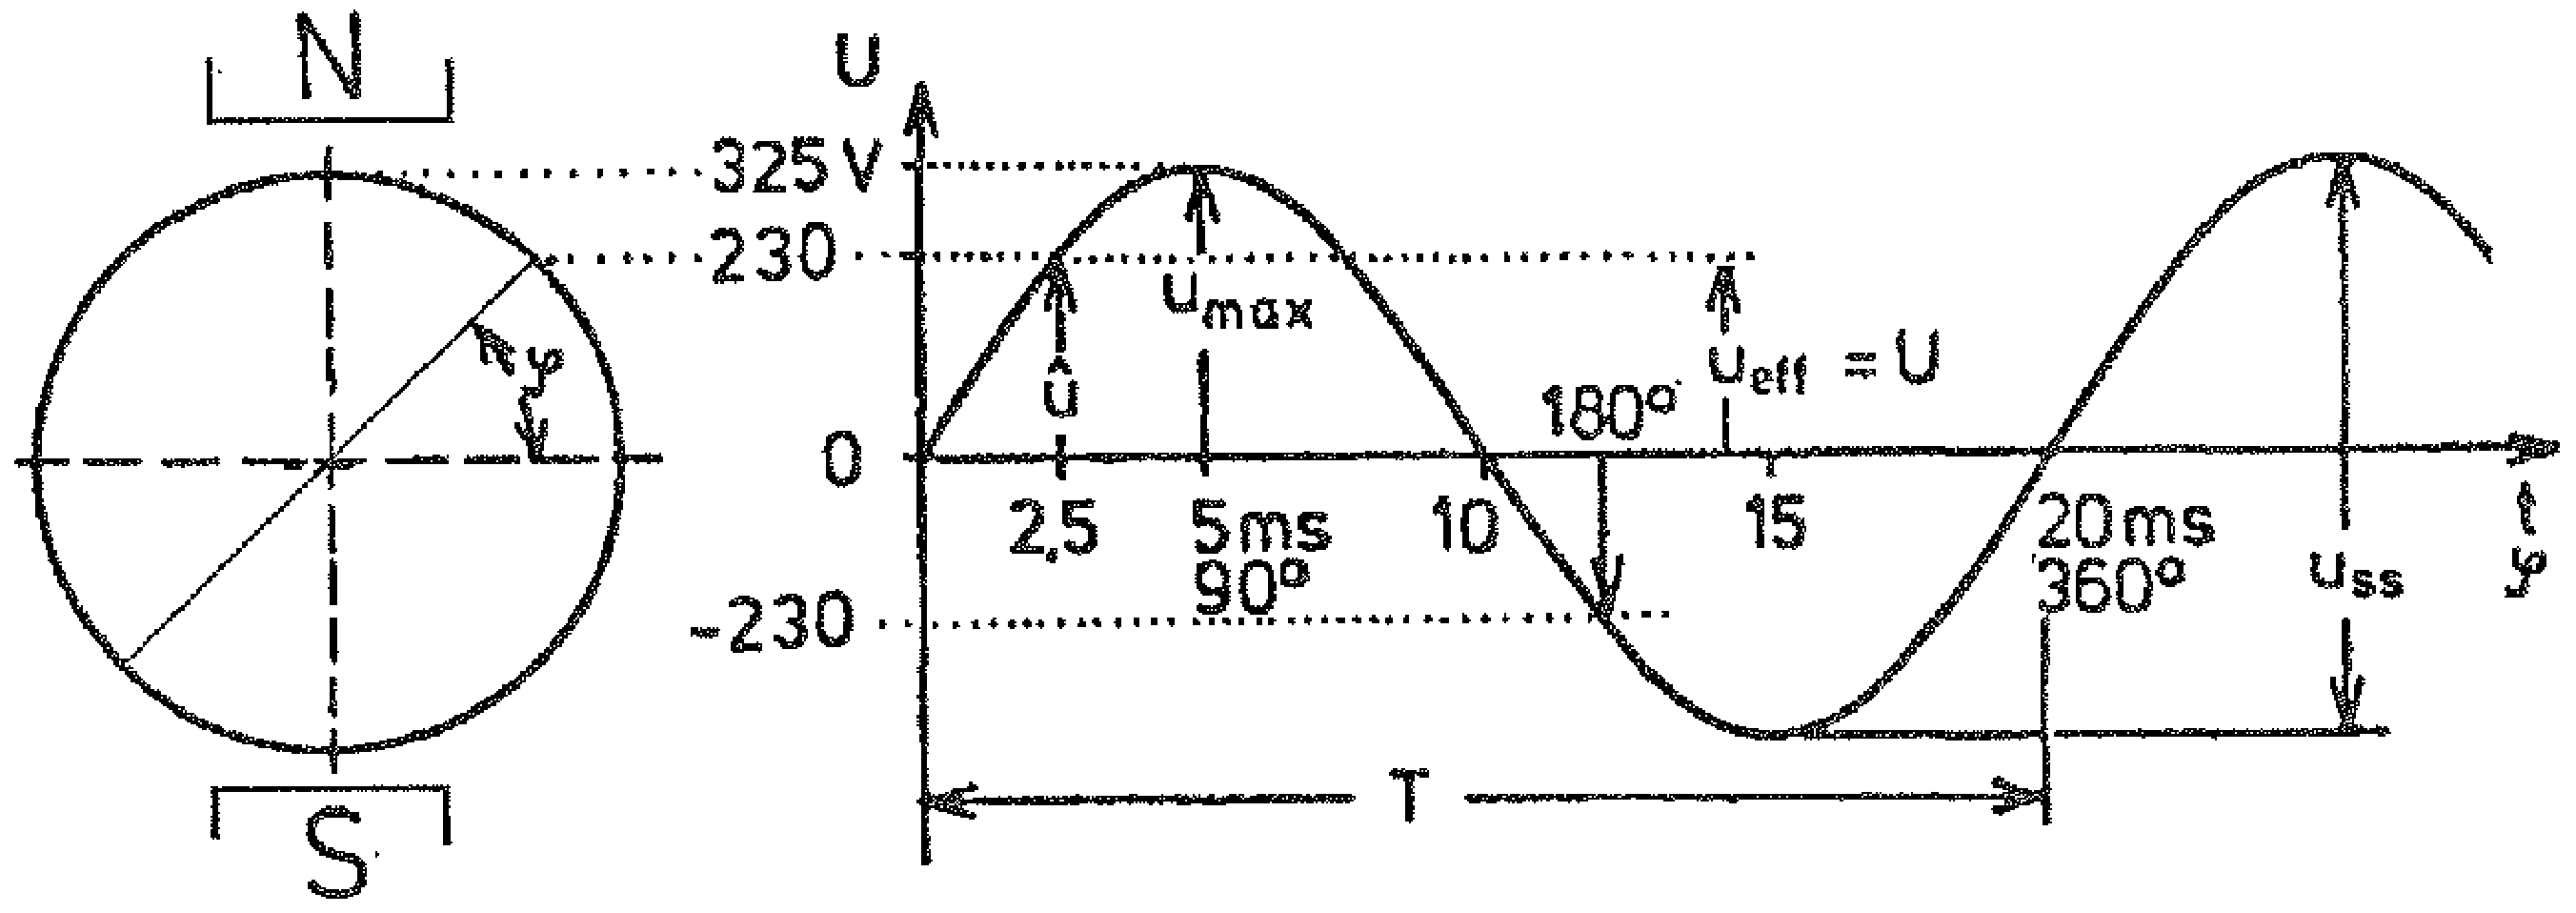
\includegraphics[width=\textwidth]{images/cropped_pdfs/bild_2_1-16.pdf}
\caption{Alstring av en sinusformad signal}
\label{fig:BildII1-16}
\end{figure}

Bild \ref{fig:BildII1-16} visar alstring av en sinusformad signal.
I detta avsnitt behandlas några grundbegrepp inom växelströmsläran.
Förloppen framställs med vektor- och linjediagram.
För närmare beskrivning används sådana begrepp som momentanvärde,
toppvärde, topp- till toppvärde, effektivvärde, fasläge, fasförskjutning och
båghastighet.

\subsection{Momentanvärde}
\textbf{HAREC a.\ref{HAREC.a.1.6.2a}\label{myHAREC.a.1.6.2a}}
\index{momentanvärde}
\index{symbol!\(u\) momentan spänning}
\index{symbol!\(i\) momentan ström}
\index{symbol!\(t\) tidpunkt}

Momentanvärdet är storheten på en spänning \(u\), en ström \(i\) etc. vid en
viss tidpunkt \(t\).
(Storheter som ändrar sig som en funktion av tiden kännetecknas ofta med gemena
bokstäver.)

Bild \ref{fig:BildII1-16} visar en sinusformad växelspänning med frekvensen
\(50\ Hz\).
Spänningen \(u\) är \(+230\ V\) vid tidpunkten 2,5~millisekunder efter en
positiv nollgenomgång.
Efter totalt \(5\, ms\) uppnås toppvärdet \(u_{max}\) d.v.s. \(+325\ V\).
Efter totalt \(10\, ms\) sker en negativ nollgenomgång.
Efter totalt \(12,5\, ms\) är spänningen \(-u\), d.v.s. \(-230\ V\) o.s.v.

\subsection{Toppvärde eller amplitud}
\textbf{HAREC a.\ref{HAREC.a.1.6.2b}\label{myHAREC.a.1.6.2b}}
\index{toppvärde}
\index{amplitud}

Toppvärdet \(u_{max}\) är det högsta värdet över eller under noll.
På bild \ref{fig:BildII1-16} är de högsta värdena \(+325\ V\) och \(-325\ V\).

\subsection{Topp-till-toppvärde}
\index{topp-till-toppvärde}

Topp-till-toppvärde är summan av toppvärdena över och under noll.
På bild \ref{fig:BildII1-16} är detta värde \(650\ V\).

\subsection{Effektivvärde}
\textbf{HAREC a.\ref{HAREC.a.1.6.2c}, a.\ref{HAREC.a.1.6.2d}\label{myHAREC.a.1.6.2c}\label{myHAREC.a.1.6.2d}}
\index{effektivvärde}

Effektivvärdet av en växelspänning \(u\) är det värde, som medför samma
effektutveckling som en likspänning \(U\).

För ett sinusformat förlopp gäller följande samband mellan toppvärdet och
effektivvärdet (det s.k. kvadratiska medelvärdet), vilket motsvarar amplituden
vid vinklarna 45, 135, 225 och 270\degree.

\(
\begin{array}{lllll}
U=\dfrac{\hat{u}}{\sqrt{2}} & & I=\dfrac{\hat{i}}{\sqrt{2}} & & (\sqrt{2} = 1,414)
\end{array}
\)

\subsection{Fasläge}
\index{fasläge}
\index{symbol!\(\phi\) fasläge}

Fasläget \(\varphi\) är när inom en period, som ett givet momentanvärde
uppträder.
Tidpunkten för varje momentanvärde motsvarar en andel av 360\degree elektriska
grader.
T.ex. uppnås värdet volt vid 0\degree, 180\degree~och 360\degree~(= 0\degree).

\subsection{Bågmått}
\index{bågmått}
\index{radianer}
\index{båghastighet (\(\omega\))}
\index{vinkelhastighet (\(\omega\))}
\index{symbol!\(\omega\) vinkelhastighet}

I beräkningar av växelströmskretsar används ofta inte vinkelmått för fasläget
(gradtal) utan i stället begreppet bågmått.

I en s.k. enhetskrets med radien \(r = 1\) motsvaras vinkeln 360\degree av en
båge med längden \(2 \cdot \pi \cdot r= 2 \cdot \pi \cdot 1 = 2 \pi =\)
omkretsen.
Vid \(f\) perioder per sekund blir båglängden \(= 2\pi f\).
Denna storhet kallas båghastigheten eller oftare vinkelhastighet och betecknas
med \(\omega\) (uttalas omega).

\(\omega= 2\pi f\) \([1/s]\)

\subsection{Period}
\textbf{HAREC a.\ref{HAREC.a.1.6.3a}\label{myHAREC.a.1.6.3a}}
\index{period}

En period har passerat, när en storhet (spänning, ström o.s.v.) återtagit samma
tillstånd eller värde efter att ha gjort en fullständig växling, t.ex. en hel
pendelrörelse eller ett helt varv vid rotation.

\subsection{Periodtid T}
\textbf{HAREC a.\ref{HAREC.a.1.6.3b}\label{myHAREC.a.1.6.3b}}
\index{periodtid (T)}
\index{symbol!\(T\) periodtid}

Periotid \(T\) är den tid som åtgår för att strömmen eller spänningen ska
genomlöpa en period. Periodtiden är det inverterade värdet av frekvensen.

Måttenheten för periodtid är sekund [s].

Periodtid

\((T) = \dfrac{1}{f}\)

\(T\ [s]  f\ [Hz]\) eller
\(T\ [ms] f\ [kHz]\) eller
\(T\ [ms] f\ [MHz]\)

Exempel:

\begin{center}
\begin{tabular}{lll}
\(T_1=\dfrac{1}{10}\) s & = 0,100 s & = 100 ms (f = 10 Hz)\\
\\
\(T_2=\dfrac{1}{50}\) s & = 0,020 s & = 20 ms (f = 50 Hz)\\
\\
\(T_3=\dfrac{1}{1000}\) s & = 0,001 s & = 1 ms (f = 1 kHz)\\
\\
\(T_4=\dfrac{1}{1000000}\) s & = 0,000001 s & = 1 \(\mu\)s (f = 1 MHz)\\
\end{tabular}
\end{center}

\subsection{Frekvens}
\textbf{HAREC a.\ref{HAREC.a.1.6.4}\label{myHAREC.a.1.6.4}}
\index{frekvens}

Frekvens är antalet perioder per tidsenhet.

Följande begrepp demonstreras med hjälp av pendeln:

Period = en fullständig fram- och tillbakasvängning i ett system, t.ex.
pendelns väg mellan punkterna 2-3-2-1-2-3- o.s.v.

\begin{figure}[ht]
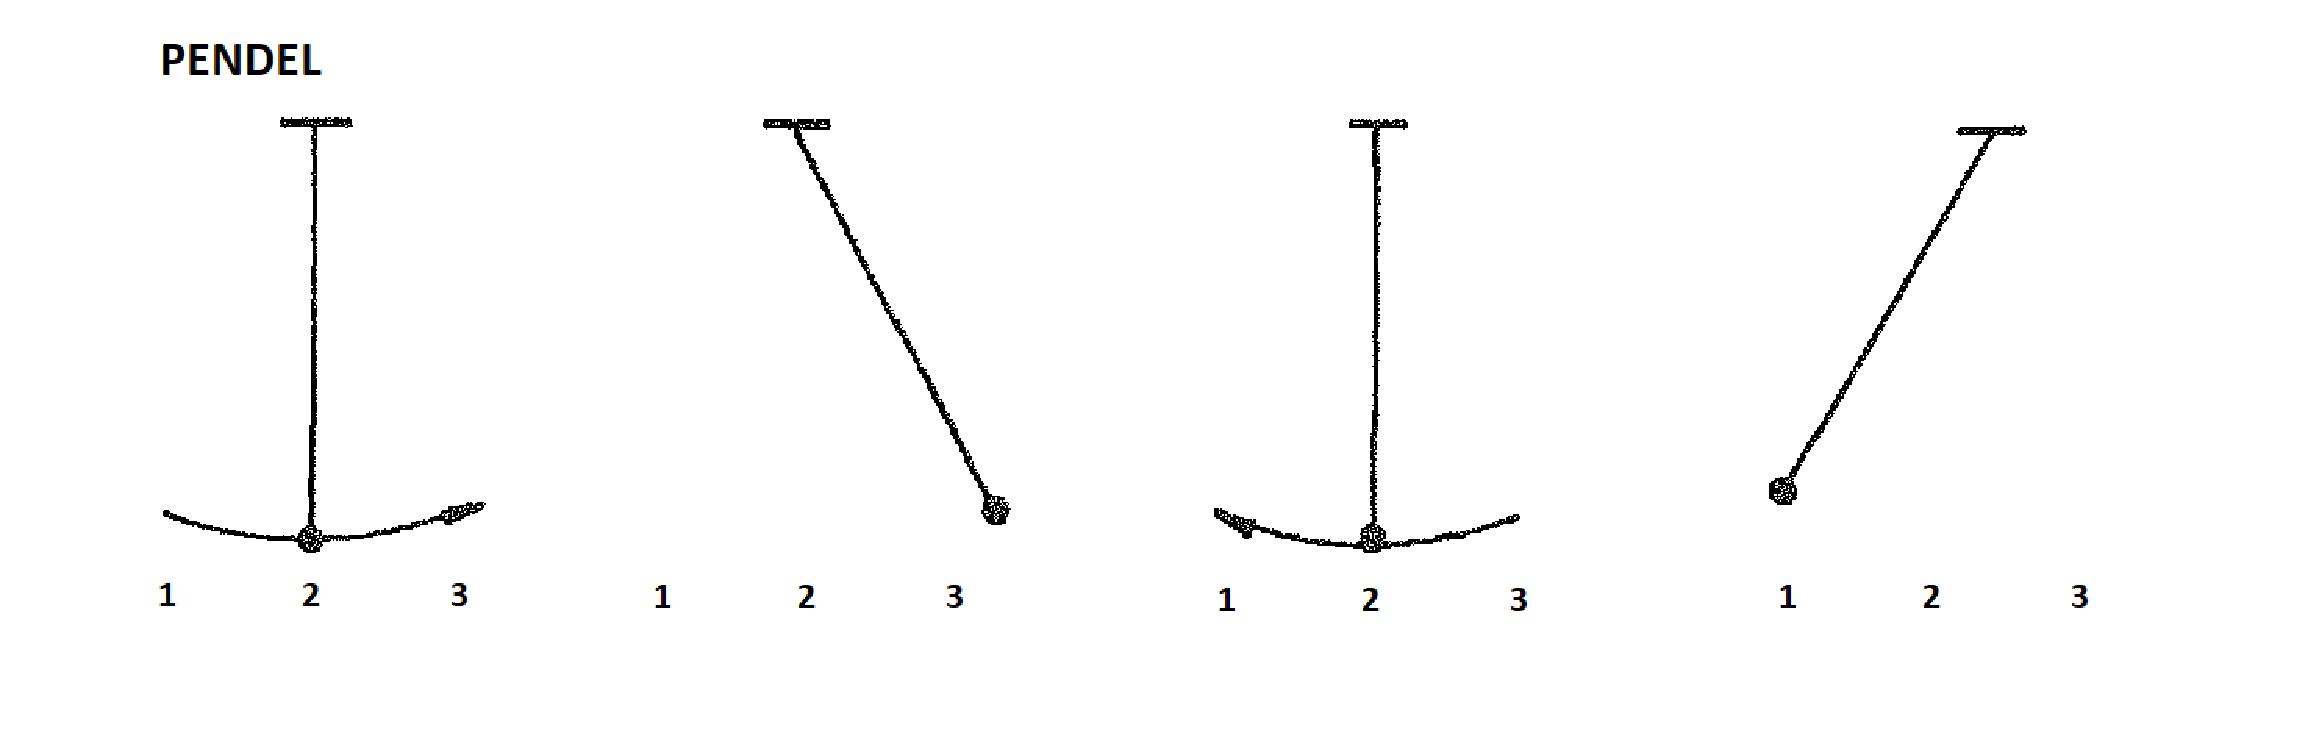
\includegraphics[width=\textwidth]{images/cropped_pdfs/bild_2_1-33.pdf}
\caption{Pendelrörelse som illustration av frekvens}
\label{fig:BildII1-33}
\end{figure}

Bild \ref{fig:BildII1-33} visar pendelrörelse som illustration av frekvens.

Periodtid \(T\) = tidsåtgången för en fullständig svängning.

Amplitud \(A\) = den största avvikelsen från viloläget.

Frekvens \(f\) = antal svängningar/tidsenhet.

Sambandet mellan frekvensen \(f\) och periodtiden \(T\) är

\(f=\dfrac{1}{T}\) t.ex.

\(5 [H z] = \dfrac{1}{5}\ [sekunder]\)

\subsection{Enheten Hertz}
\textbf{HAREC a.\ref{HAREC.a.1.6.5}\label{myHAREC.a.1.6.5}}
\index{Hertz}
\index{enheter!Hertz (Hz)}
\index{symbol!\(f\) frekvens}

Måttenheten för frekvens är Hertz [Hz].
I formler betecknas frekvensen med \(f\).

\begin{center}
\begin{tabular}{ll}
1~Hz      & = 1 period per sekund (p/s) \\
10~Hz     & = 10 perioder per sekund \\
50~Hz     & = 50 perioder per sekund \\
1~000~Hz  & = \(10^3\)~Hz = 1~kHz (kilohertz) \\
1~000~kHz & = \(10^6\)~Hz = 1~MHz (megahertz) \\
1~000~MHz & = \(10^9\)~Hz = 1~GHz (gigahertz) \\
\end{tabular}
\end{center}

Nätfrekvensen för elkraft är i Europa 50~Hz.

Andra nätfrekvenser förekommer, t.ex. 60~Hz i USA och Japan.

Frekvensområdet vid överföring av kvalitativt tal och musik, lågfrekvens LF, är
mellan ca 16~Hz och 16~kHz.

Frekvensområdet för talöverföring, t.ex. över telefonlinjer eller
kommunikationsradio, är ca 300 till 3000~Hz.

Frekvensområdet för radioöverföring, högfrekvens HF, är i huvudsak mellan
50~kHz, s.k. långvåg, och 100-tals GHz, s.k. mikrovåg.

\subsection{Fasförskjutning}
\textbf{HAREC a.\ref{HAREC.a.1.6.6}\label{myHAREC.a.1.6.6}}
\index{fasförskjutning}

\begin{figure}[ht]
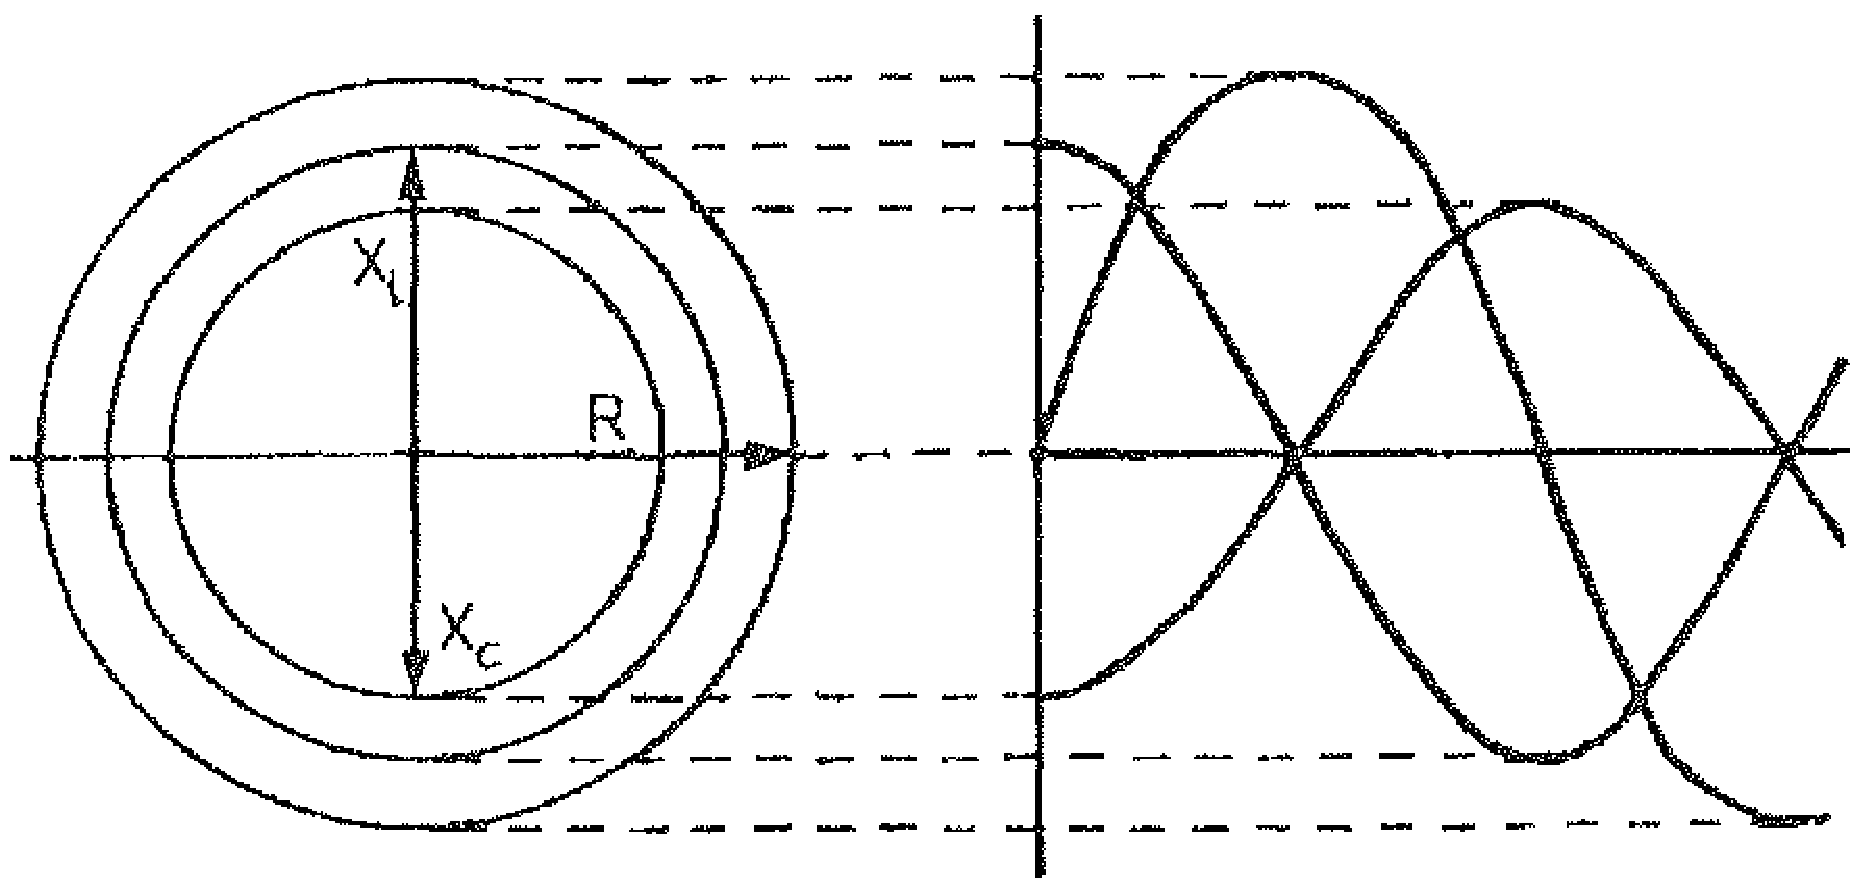
\includegraphics[width=\textwidth]{images/cropped_pdfs/bild_2_1-17.pdf}
\caption{Vektorer och fasförskjutning}
\label{fig:BildII1-17}
\end{figure}

Bild \ref{fig:BildII1-17} visar vektorer och fasförskjutning.
Med fasförskjutning menas tidsskillnaden mellan förlopp, t.ex. spänningar
och/eller strömmar.
Fasförskjutningen mellan vektorerna kallas även fasvinkel och uttrycks som ett
gradtal mellan 0 och 360\degree.

\subsection{Vektorer}
\index{vektorer}

En spänning, ström, kraft o.s.v. kan beskrivas som en vektor med en storhet och
riktning.
På bilden \ref{fig:BildII1-17} har vektorerna \(X_L\), \(R\) och \(X_C\) en
inbördes fasförskjutning av 90\degree.
De motsvarar spänningsfallen i en krets med en induktor, en resistor och en
kondensator kopplade i serie, där den gemensamma strömmen är en sinus.

Antag att vektorerna roterar i ett oförändrat inbördes läge och med en
vinkelhastighet av \(\omega= 2\pi f\).
Systemet roterar då \(360\degree = 2\pi\ radianer = 1\ varv/period\).

Vid varje tidpunkt har vektorsystemet uppnått en viss vridningsvinkel.
Momentanvärdet på vektorernas spänningar avsätts till höger i bilden.
Avståndet mellan en vektorspets och noll-linjen är vektorns momentana värde,
som kan vara positivt eller negativt.

%\cleardoublepage
%\section{Icke sinusformade signaler}
\textbf{HAREC a.\ref{HAREC.a.1.7}\label{myHAREC.a.1.7}}

\subsection{Grundton, övertoner- Kantvågor}
\textbf{HAREC a.\ref{HAREC.a.1.7.2}, a.\ref{HAREC.a.1.7.3}, a.\ref{HAREC.a.1.7.4b}\label{myHAREC.a.1.7.2}\label{myHAREC.a.1.7.3}\label{myHAREC.a.1.7.4b}}
\index{grundton}
\index{överton}
\index{kantvåg}

\begin{figure*}
\begin{center}
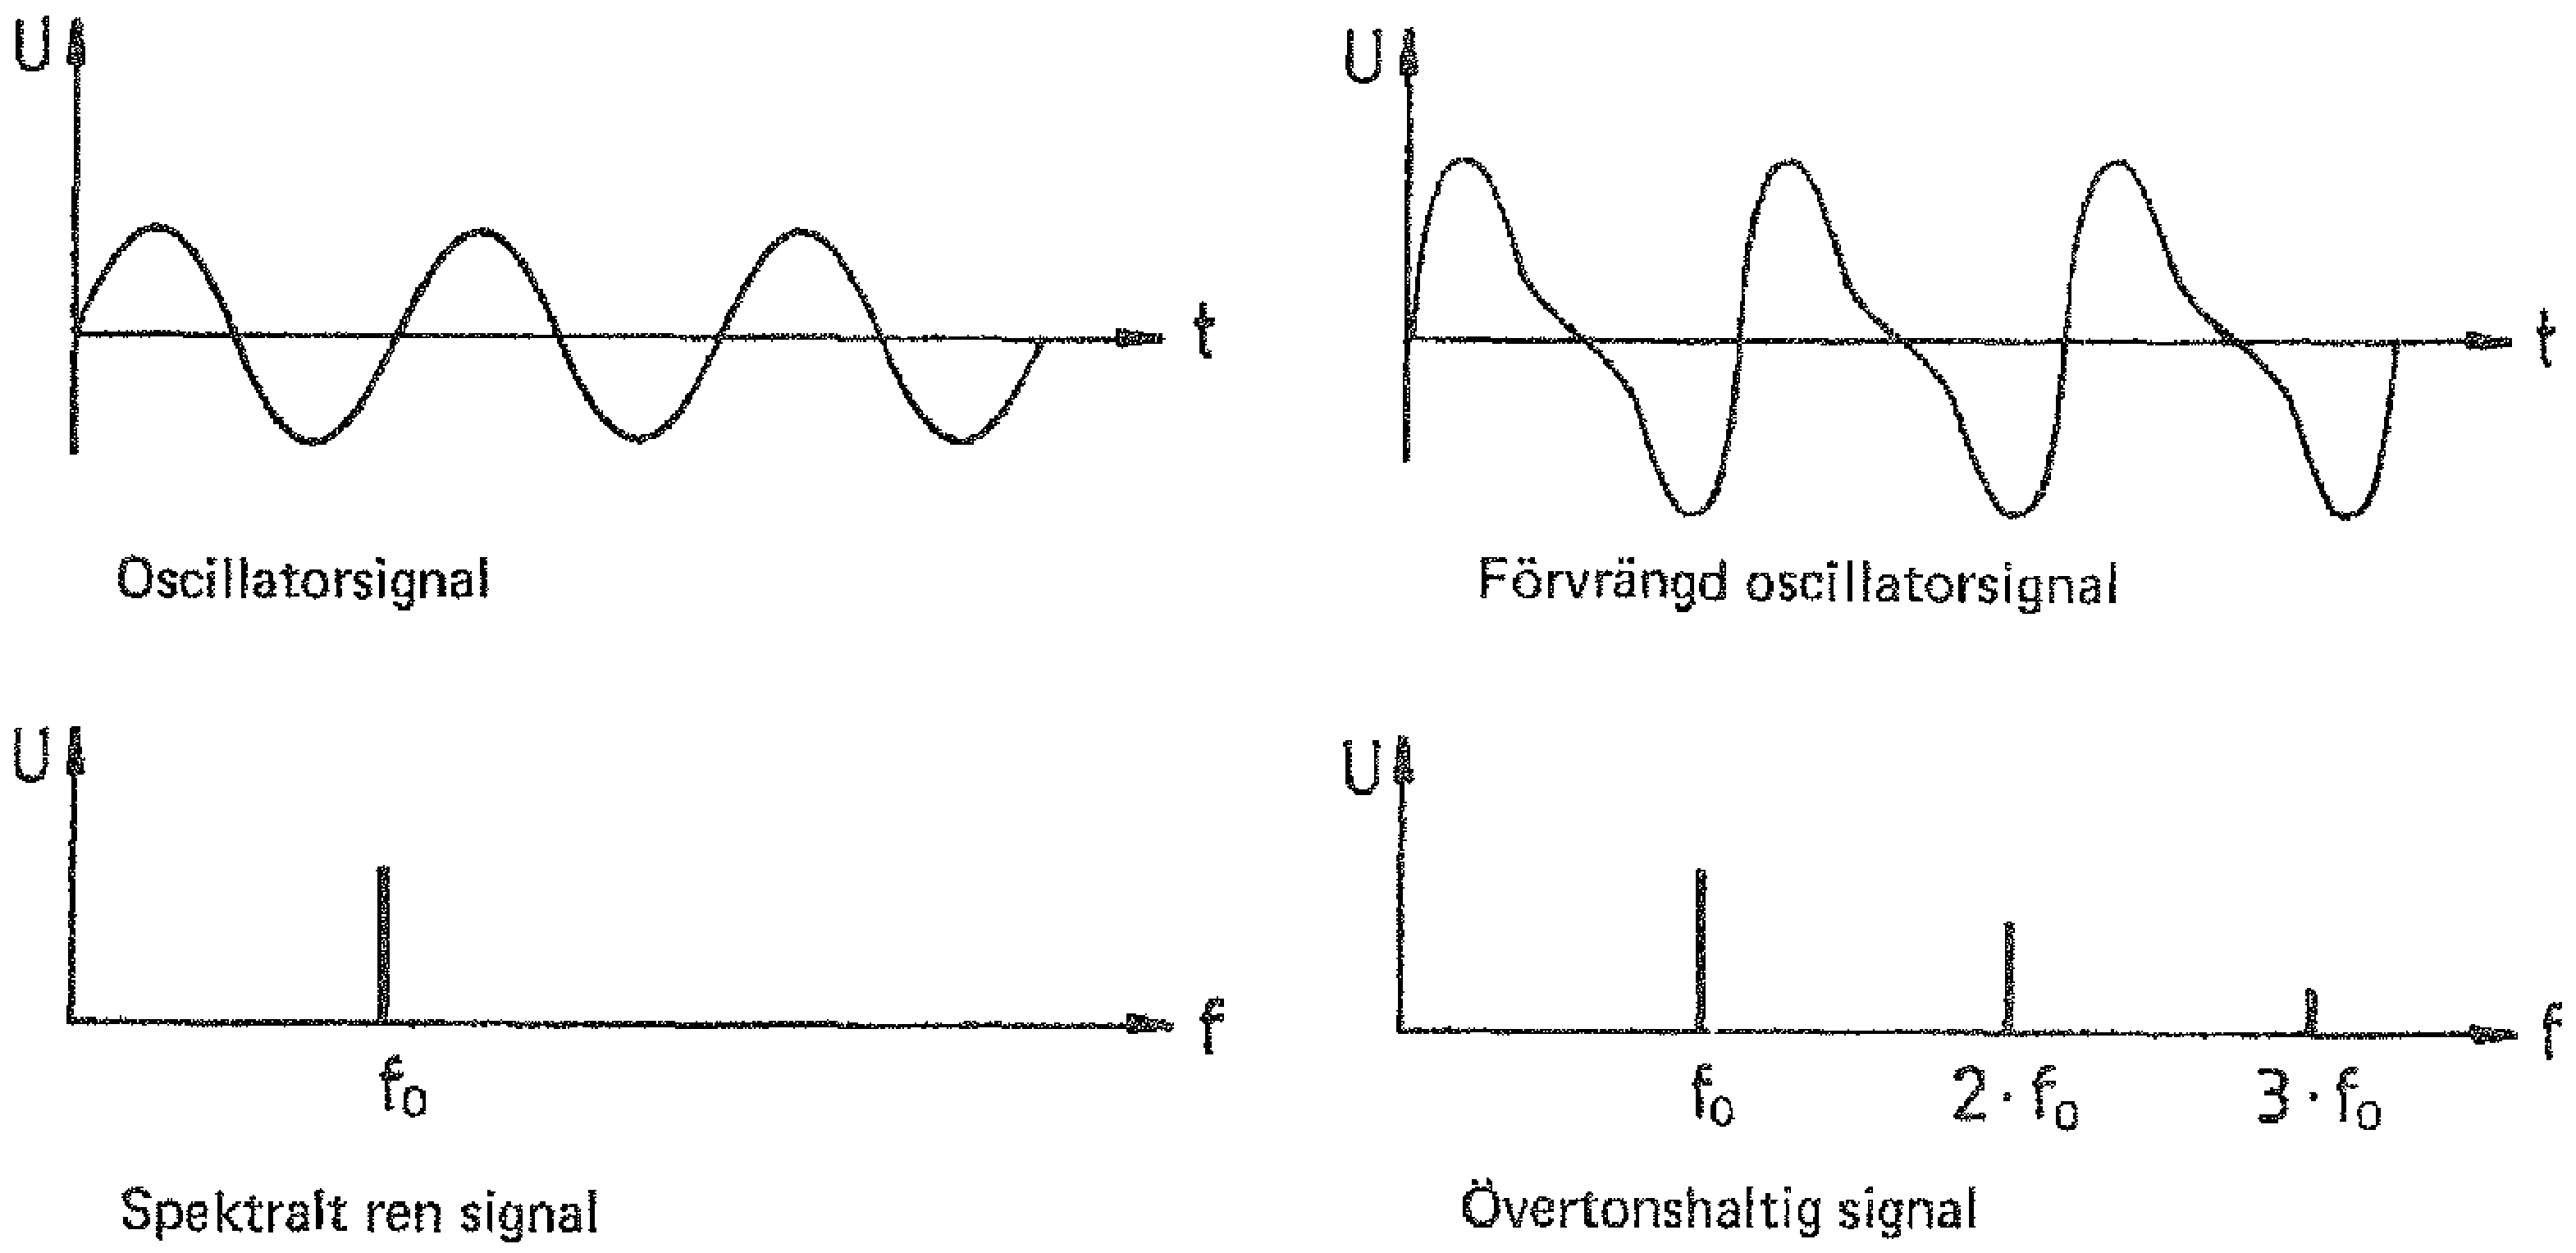
\includegraphics[width=\textwidth]{images/cropped_pdfs/bild_2_1-18.pdf}
\caption{Ren sinusvåg och övertonshaltig våg}
\label{fig:BildII1-18}
\end{center}
\end{figure*}

Bild \ref{fig:BildII1-18} visar en ren sinusvåg och övertonshaltig våg.
Ett sinusformat förlopp med en enda frekvens -- en enda ton -- sägs vara
spektralt ren.
En sådan svängning kallas för grundton.

Varje signal, som inte är sinusformad, är sammansatt av flera sinussvängningar.
Det är signalens grundton samt dess harmoniska övertoner, vilka kan ha 2, 3
o.s.v. gånger högre frekvens än grundtonen.
Den inbördes styrkan på grundton och övertoner avgör signalens form.
Om signalen ligger inom det hörbara området, kan man märka hur den ändrar
karaktär beroende på övertonshalten.
Man kan säga att övertonerna modulerar grundtonen.

\begin{figure*}
\begin{center}
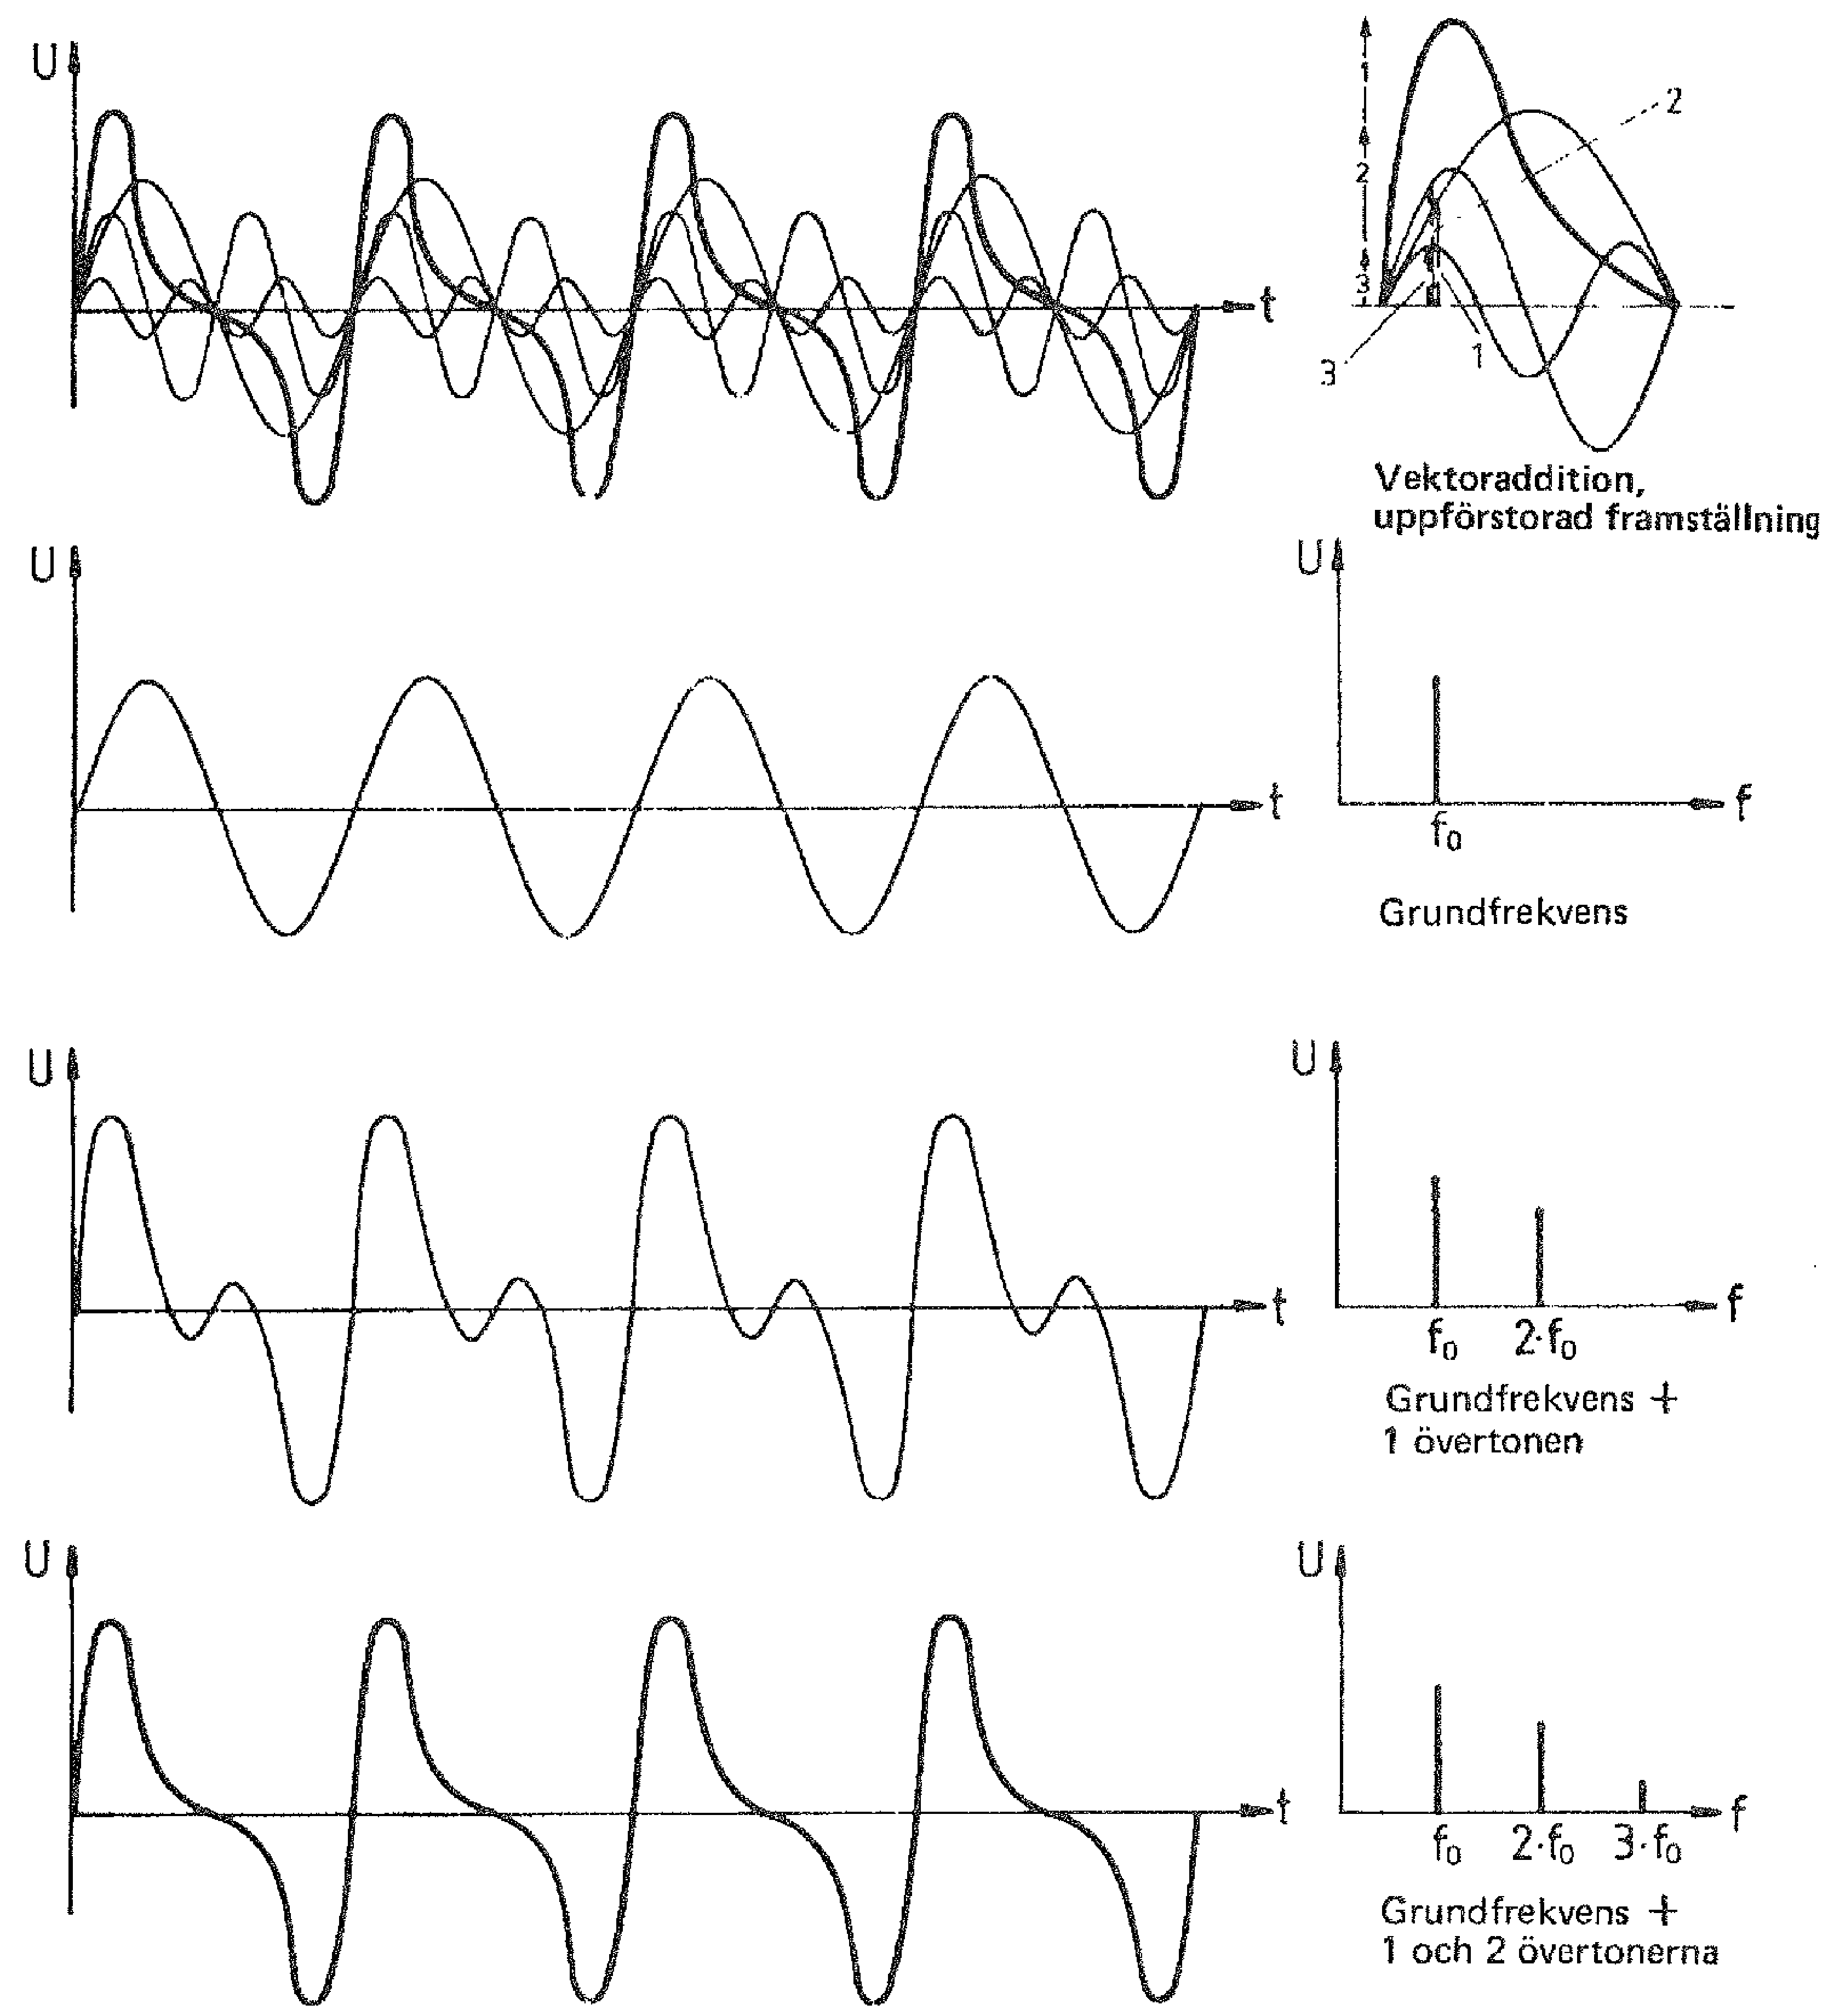
\includegraphics[width=\textwidth]{images/cropped_pdfs/bild_2_1-19.pdf}
\caption{Uppdelning av en signal i grundton och övertoner}
\label{fig:BildII1-19}
\end{center}
\end{figure*}

Bild \ref{fig:BildII1-19} visar uppdelning av en signal i grundton och
övertoner.
Oscillatorsignalen i exemplet på bilden har 1 volts amplitud på grundtonen
\(f_0\) (1:a harmoniska), 0,7~volts amplitud på de 1:a övertonen
(2:a harmoniska) och 0,2~volts amplitud på den 2:a övertonen (3:e harmoniska).
Den totala amplituden blir emellertid inte summan av 1, 0,7 och 0,2~volt
eftersom de olika delspänningarnas toppvärden inte uppträder samtidigt.
I stället måste delspänningarna adderas vid varje tidpunkt för sig.

\begin{figure*}
\begin{center}
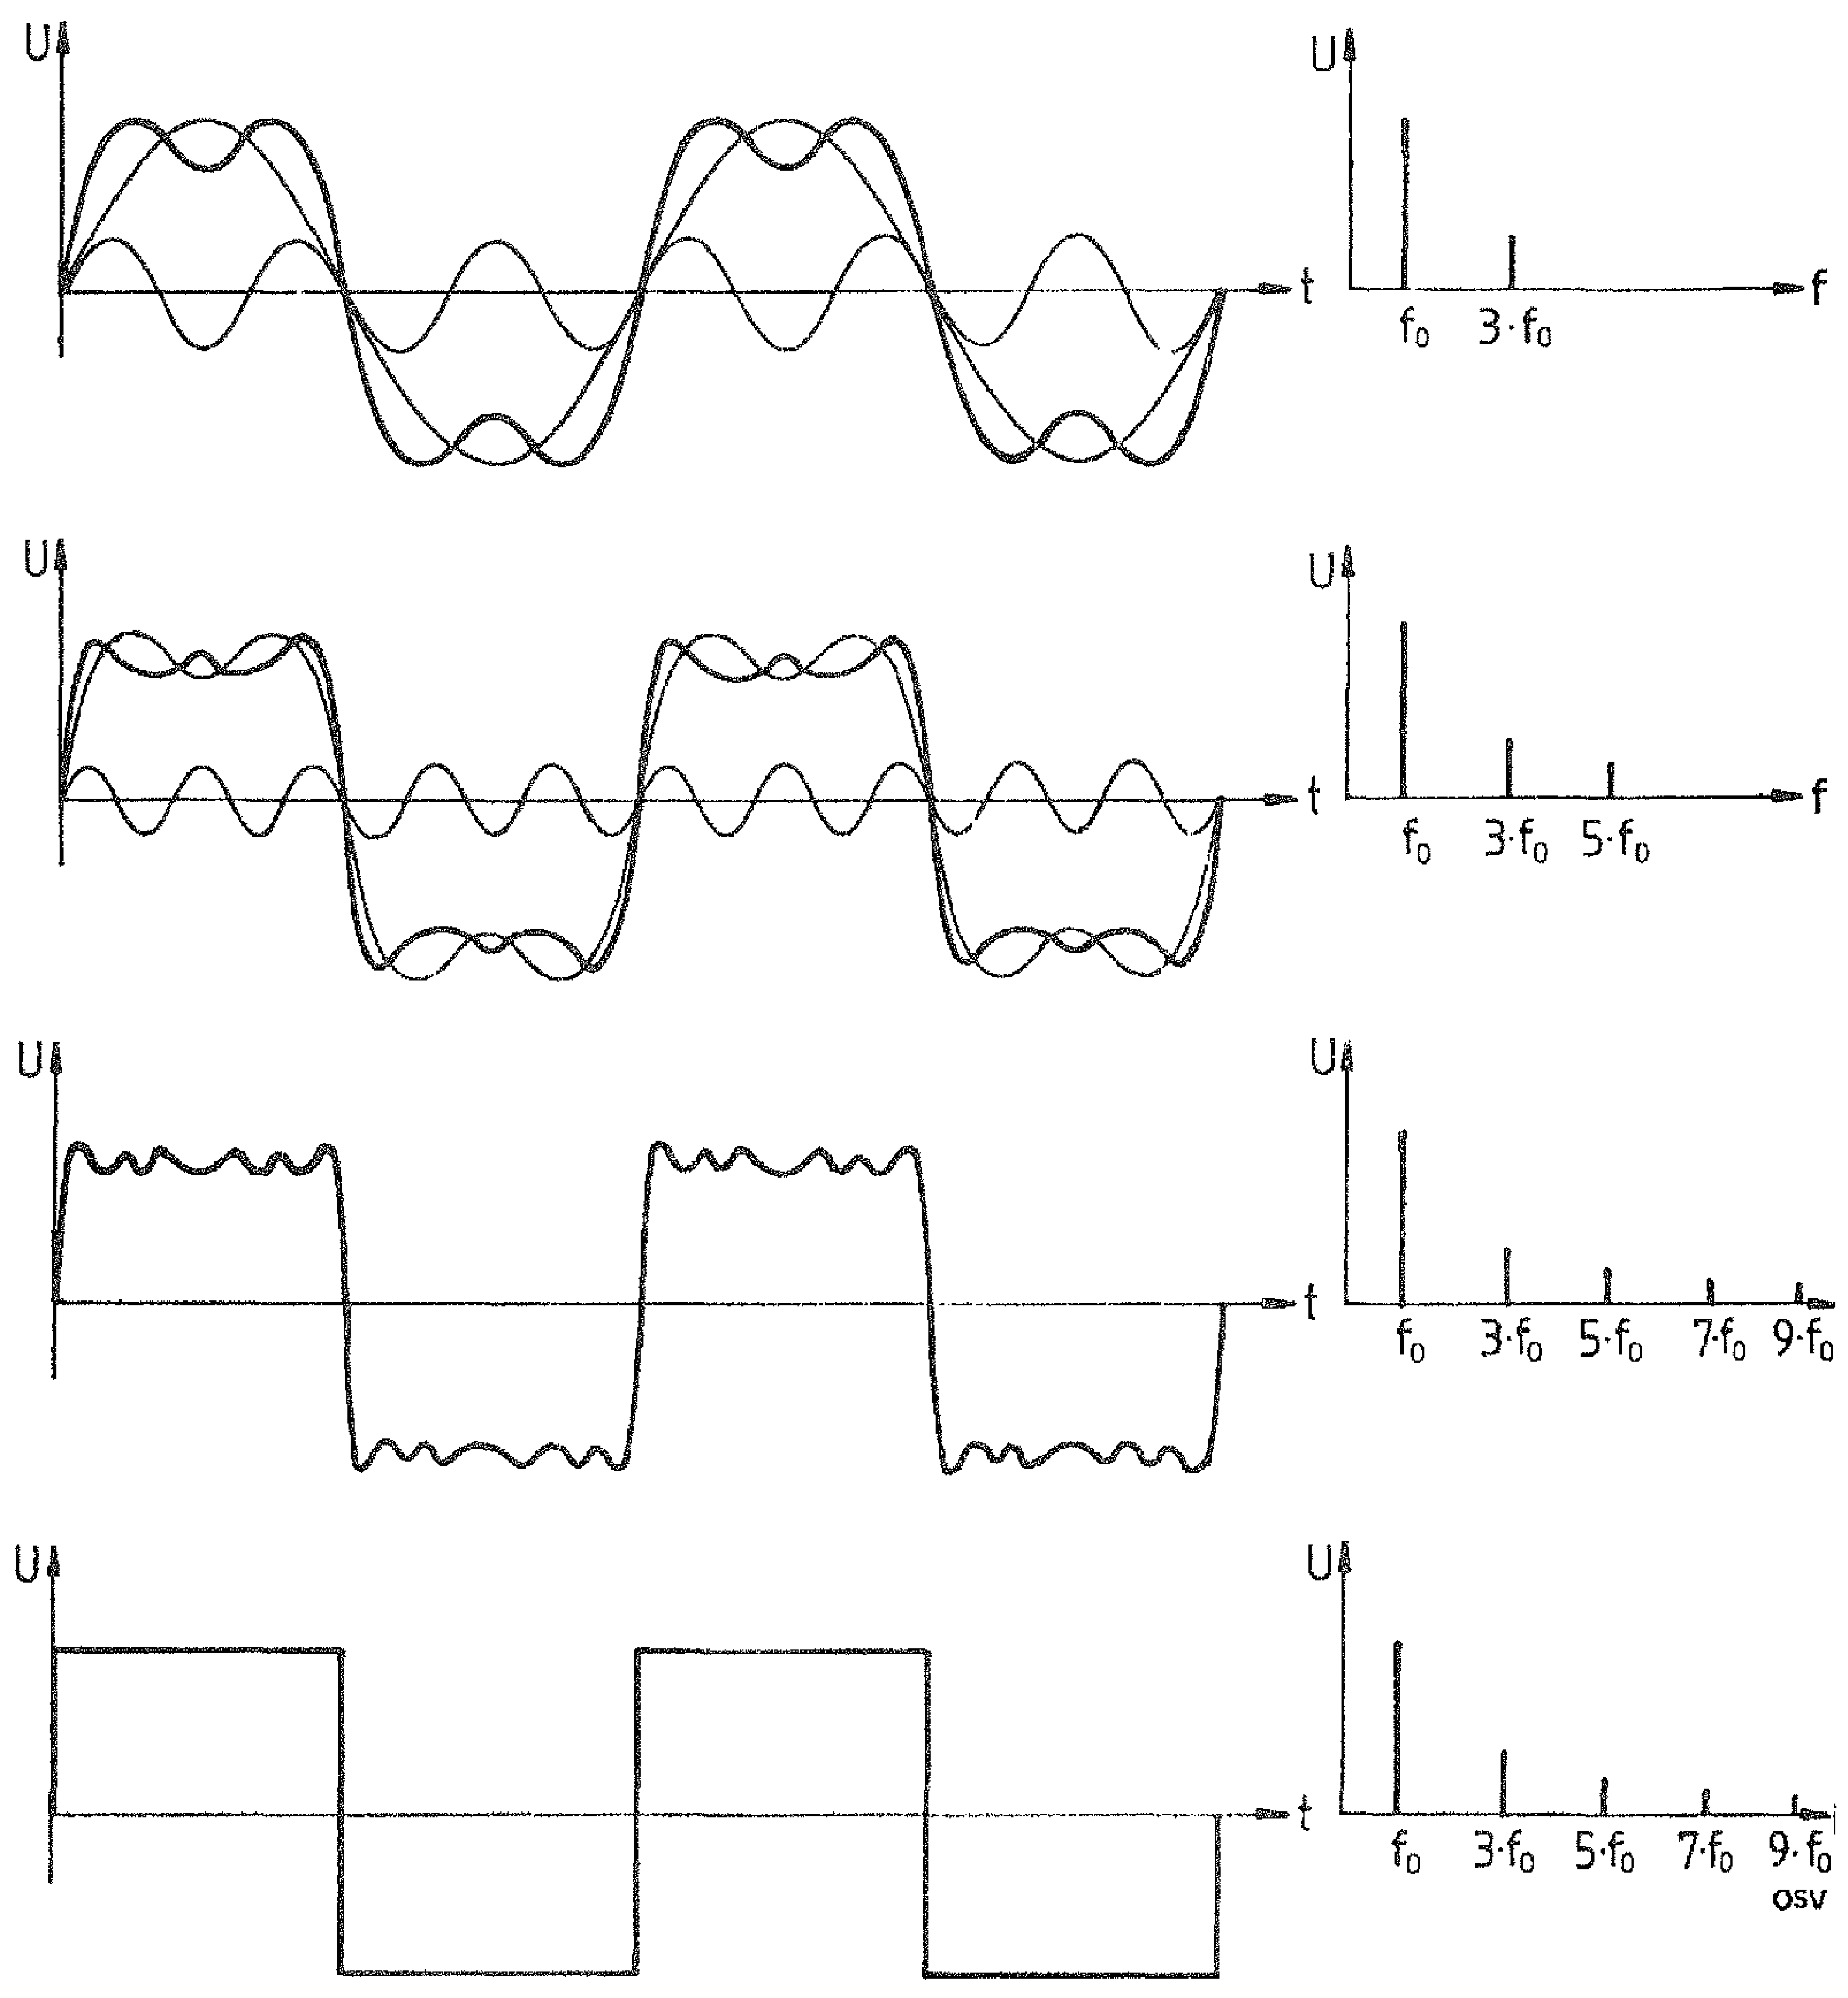
\includegraphics[width=\textwidth]{images/cropped_pdfs/bild_2_1-20.pdf}
\caption{Uppdelning av en fyrkantsvåg i grundton och övertoner}
\label{fig:BildII1-20}
\end{center}
\end{figure*}

Bild \ref{fig:BildII1-20} visar uppdelning av en fyrkantsvåg i grundton och
övertoner.

\index{Fourier, Joseph}
\index{Fourier!Fourier analys}
\index{Fourier!Fourier transform (FT)}
\index{Fourier!invers Fourier transform (IFT)}
\index{Fourier!Discrete Fourier Transform(DFT)}
\index{DFT}
\index{Fourier!inverse Discrete Fourier Transform (IDFT)}
\index{IDFT}
\index{Fourier!Fast Fourier Transform(FFT)}
\index{FFT}
\index{Fourier!inverse Fast Fourier Transform (IFFT)}
\index{IFFT}

\infobox{
Denna analys av vågor uppfanns av Jean-Baptiste Joseph Fourier (1768--1830)
vid analys av värmeutbredning och vibration som presenterades 1822.
Denna metod är kraftfull och har haft stort inflytande på vetenskapen och
utvecklingen både som matematiskt verktyg och som praktiskt analys med
spektrum-analysatorer och vid modern modulation och demodulation.
Man pratar om \emph{Fourier analys} (eng. Fourier analysis) och
\emph{Fourier transform (FT)} för omvandling från tid till frekvens och
\emph{invers Fourier transform} för omvandling från frekvens till tid.
För tidsdiskret (samplad) form är termerna
\emph{Diskret Fourier Transform (DFT)} och
\emph{invers Diskret Fourier Transform (IDFT)} respektive.
Senare optimeringar av beräkningar har resulterat i
\emph{Fast Fourier Transform (FFT)} och
\emph{Inverse Fast Fourier Transform (IFFT)}.
}

Det finns olika karaktärer av förlopp såsom sinusvåg, triangelvåg, sågtandsvåg,
fyrkantsvåg o.s.v.

Fyrkantsvågen är sammansatt av sinusvågor med grundfrekvensen och dess udda
övertoner, varvid amplituderna fördelar sig som \(1/1\), \(1/3\), \(1/5\),
\(1/7\), \(1/9\), \(1/11\) o.s.v.
Teoretiskt når övertonsspektrum upp till oändligt höga frekvenser, medan de
motsvarande amplituderna minskar till oändligt små värden.

En ideal fyrkantsvåg, vilken inte kan uppnås i praktiken, skulle bestå av ett
oändligt antal udda övertoner med fallande amplitud.
Ju fler av de högre övertonerna som filtreras bort, desto mer lutar
fyrkantsvågens flanker, desto rundare blir hörnen på vågen och desto vågigare
blir kurvans topp.

\subsection{Överlagrade spänningar
(likspänningskomposant)}
\textbf{HAREC a.\ref{HAREC.a.1.7.4a}\label{myHAREC.a.1.7.4a}}

\begin{figure}[ht]
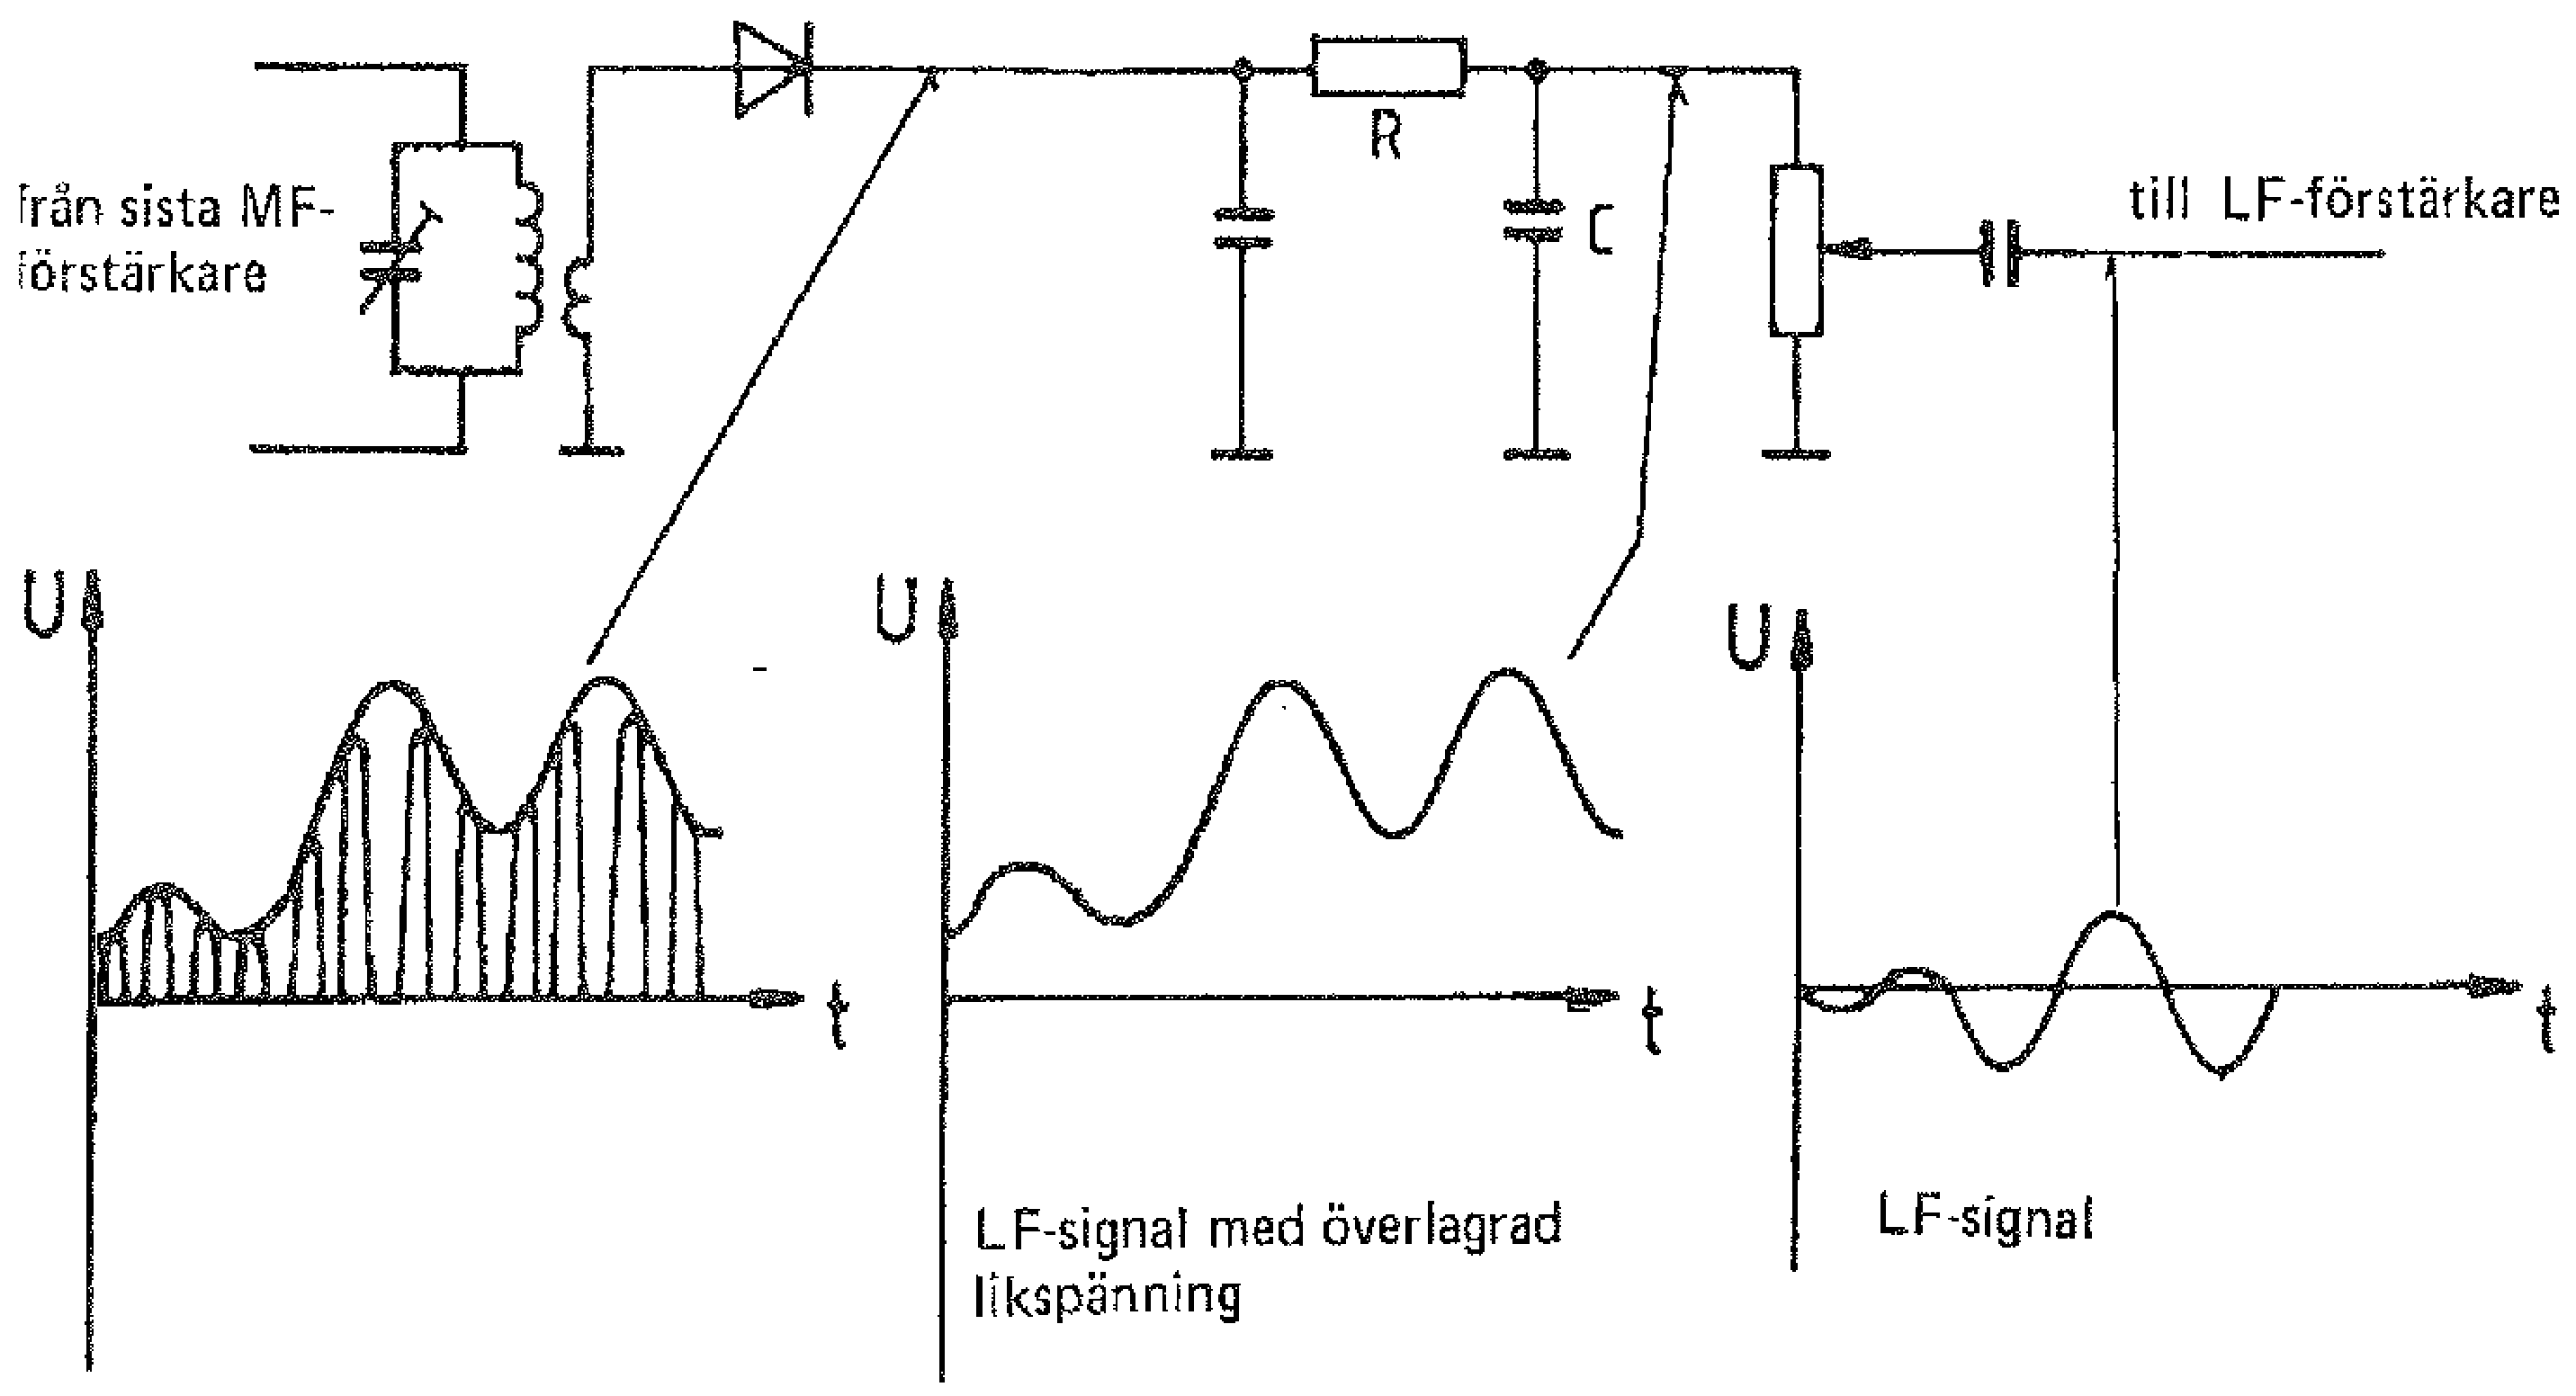
\includegraphics[width=\textwidth]{images/cropped_pdfs/bild_2_1-21.pdf}
\caption{Överlagrade spänningar}
\label{fig:BildII1-21}
\end{figure}

Bild \ref{fig:BildII1-21} visar överlagrade spänningar.
I signalkretsar förekommer det mycket ofta, att växelspänning överlagras på
likspänning eller omvänt.
Likspänningen kallas då för likspänningskomposant.
Olika åtgärder behövs för att överlagra spänningar på varandra och att sedan
skilja dem åt.

Bilden visar ett avsnitt av en AM-mottagare.
Från vänster hämtas en AM-modulerad signal från MF-förstärkaren för att
demoduleras, d.v.s. för att återvinna den modulerande LF-signalen.
MF-signalen halvvågslikriktas.
Kvar blir den positiva delen av MF-signalen och den modulerande LF-signalen,
sammanlagrade.
LF-signalen ska nu skiljas ut och förstärkas.
Alltså filtreras MF-komposanten bort.
Kvar blir LF-signalen, men överlagrad på en likspänning.
Likspänningen stoppas och kvar blir slutligen LF-signalen som förstärks.

\subsection{Brus}
\textbf{HAREC a.\ref{HAREC.a.1.7.5}\label{myHAREC.a.1.7.5}, a.\ref{HAREC.a.7.19}\label{myHAREC.a.7.19}}
\label{termisktbrus}

\subsubsection{Termiskt brus}
\index{brus}
\index{termiskt brus}
\index{brus!termiskt}

Resistorer och resistans, i alla dess former, uppvisar en egenskap av
en varierande spänning även när ingen ström går genom motståndet.
Denna extra spänning innehåller ett brett spektra av toner, men är också ett
tätt spektra, sådan att ingen enskild ton kan särskiljas från någon annan.
Istället för att tänka sig en grundton och dess övertoner med ingen energi
emellan dem så är det istället ett kontinuerligt spektra med oändligt många
toner.
Detta spektra begränsas dock av bandbredden.

\begin{wrapfigure}{R}{0.5\textwidth}
  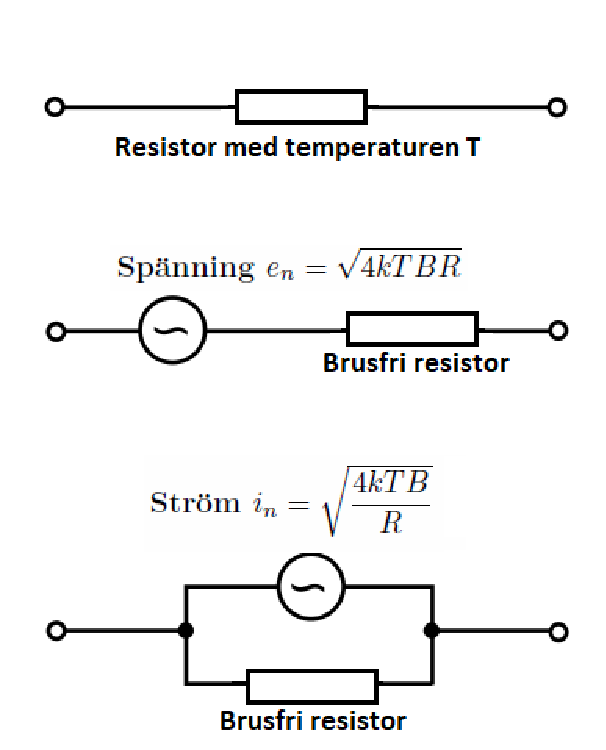
\includegraphics[width=0.5\textwidth]{images/cropped_pdfs/bild_2_1-36.pdf}
  \caption{En resistor kan ses ha brus ekvivalenter som spänning eller ström}
  \label{fig:BildII1-36}
\end{wrapfigure}

\begin{wrapfigure}{R}{0.5\textwidth}
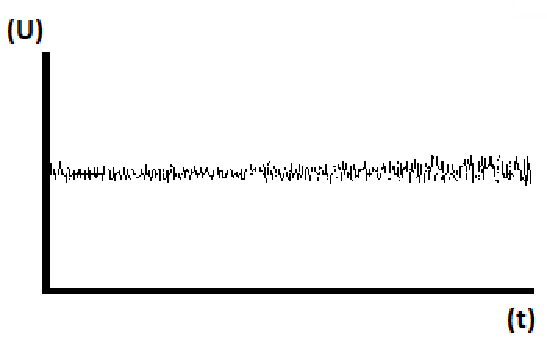
\includegraphics[width=0.5\textwidth]{images/cropped_pdfs/bild_2_1-34.pdf}
\caption{Brus innebär en ostabilitet över tid}
\label{fig:BildII1-34}
\end{wrapfigure}

\begin{wrapfigure}{R}{0.5\textwidth}
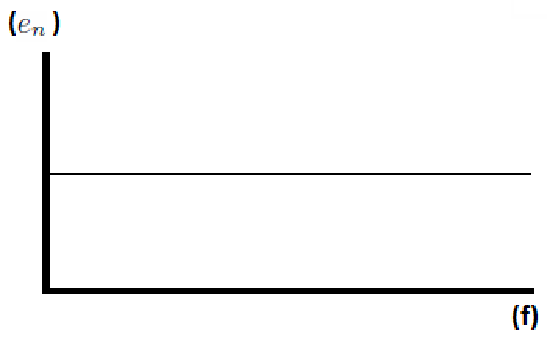
\includegraphics[width=0.5\textwidth]{images/cropped_pdfs/bild_2_1-35.pdf}
\caption{Brus innehåller alla frekvenser, vitt brus har samma amplitud}
\label{fig:BildII1-35}
\end{wrapfigure}

\index{vitt brus}
\index{brus!vitt}
\index{white noise}
\index{Johnsson noise}
\index{brus!Johnsson}
Man kallar detta spektra i daglig tal för \emph{termiskt brus}
(eng. thermal noise), eftersom det beror på temperaturen hos motståndet, eller
\emph{Johnsson noise}, efter J. B. Johnsson som 1928 fann att detta brus fanns
i alla ledare \cite{ott1988}.
Brus skapar en variation i spänning och ström, som illustreras i bild
\ref{fig:BildII1-34}.

I dagligt tal pratar man dock bara om \emph{vitt brus} (eng. white noise) eller
\emph{brus}.
Med vitt brus menas brus som inte ''färgats'', och det betyder i det här
sammanhanget att det har samma amplitud för alla frekvenser, så som illustreras
i bild \ref{fig:BildII1-35}.
I praktiken är allt brus begränsat med bandbredden på kanalen, men man
betraktar det som vitt inom kanalen om det är jämn inom bandet.

Effekten \(P_n\) av detta brus beror på Boltzmanns konstant
\(k\ =\ 1,38 \cdot 10^{-23}\) J/K, den absoluta temperaturen \(T\) i
kelvin samt bandbredden \(B\) i hertz och anges enligt formeln:

\(P_n = k T B\)

Varje motstånd med den absoluta temperaturen T kan modelleras som att ha en
ekvivalent spänning \(e_n\) och ström \(i_n\) för resistansen \(R\),
så som illustreras i bild \ref{fig:BildII1-36} är

\(e_n = \sqrt{4kTBR}\)

\(i_n = \sqrt{\dfrac{4kTB}{R}}\)

\subsubsection{Brusbandbredd}
\index{brus!brusbandbredd}

Medans vi initialt antagit att brusets bandbredd är för frekvenser
från DC till övre gränsfrekvensen så är det inte nödvändigt.
Formeln är även relevant för bruset på ett band, och bandbredden för det
bandpass filter vi har för att enbart lyssna på detta band.

Exempelvis behöver tal på SSB hantera 300~Hz till 3~kHz, dvs. 2,7~kHz
bandbredd och därmed kommer även mottagarens bandbredd behöva vara så stort,
och därmed även brusbandbredd på 2,7~kHz.
Vi kommer då att ta emot brus för motsvarande bandbredd.
Ett CW filter kan t.ex. vara 350~Hz och kommer därmed också ha ett
motsvarande förhållande lägre brus-effekt.

Detta är dock en förenkling, eftersom filtret inte filtrerar med branta kanter
och är helt plant.
Filtrets egentliga brus-bandbredd beror på hur filtret filtrerar över
alla frekvenser och summan av dessa.
Beroende på vilken typ av filter så behövs därför en korrigeringsfaktor
från den normala bandbredden till brus-bandbredden.
För ett normalt 12~dB/oktav lågpassfilter är korrigeringsfaktorn 1,22.

%\cleardoublepage
%\section{Modulation}
\textbf{HAREC a.\ref{HAREC.a.1.8}\label{myHAREC.a.1.8}}
\label{modulation}
\index{modulation}

\subsection{Allmänt}

\emph{Modulera} (lat. \emph{modulari}, rytmiskt avmäta) är att med hjälp av en
oftast högfrekvent elektrisk signal (bärvågen) överföra informationen i en
lågfrekvent signal. På så sätt kan lågfrekvens, t.ex. tal och musik, först
omvandlas till en elektrisk signal, som får påverka (modulera) en högfrekvent
elektrisk signal. Denna modulerade signal strålas ut från antennen som ett
elektromagnetiskt fält.

Den signal som innehåller informationen kallas \emph{modulerande signal} eller
\emph{basband} eller \emph{underbärvåg}.

Den signal som informationen överförts till kallas \emph{modulerad signal}
eller \emph{huvudbärvåg}.

\subsection{Modulationssystem}

Den största gruppen av modulationssystem är definierad med avseende på hur
huvudbärvågen är modulerad. Vanligast är då amplitud- och vinkel modulation.
Av vinkelmodulation finns främst två slag, frekvensmodulation och
fasmodulation. Därutöver finns system för pulsmodulation.

\subsection{Sändningsslag}
\index{sändningsslag}

Sätten att modulera kallas \emph{sändningsslag}. Gemensamt för sändningsslagen
är att en givare -- det kan vara en mikrofon, en telegrafnyckel, en
fjärrskriftsmaskin, en dator, en TV-kamera o.s.v. -- alstrar en analog eller
digital signal. Denna styr underbärvågen så att huvudbärvågen moduleras med den
avsedda informationen och sänds ut.

Det enklaste sändningsslaget får anses vara morsetelegrafi med ''nycklad bärvåg''.
Då förekommer bara två tillstånd, nedtryckt och icke nedtryckt telegrafnyckel,
d.v.s. antingen bärvåg med någon varaktighet eller ingen bärvåg alls.
Kombinationer av bärvågselement med olika längd motsvarar skrivtecken.

För att återge tal, musik etc. behövs en noggrannare tillståndsstyrning av
bärvågen. Det innebär att bärvågen måste moduleras av en underbärvåg och att
denna motsvarar lufttrycksvariationerna i ljudet.

\subsection{Kännetecken för modulerade signaler}
\textbf{HAREC a.\ref{HAREC.a.1.8.5}\label{myHAREC.a.1.8.5a}}

\begin{figure}
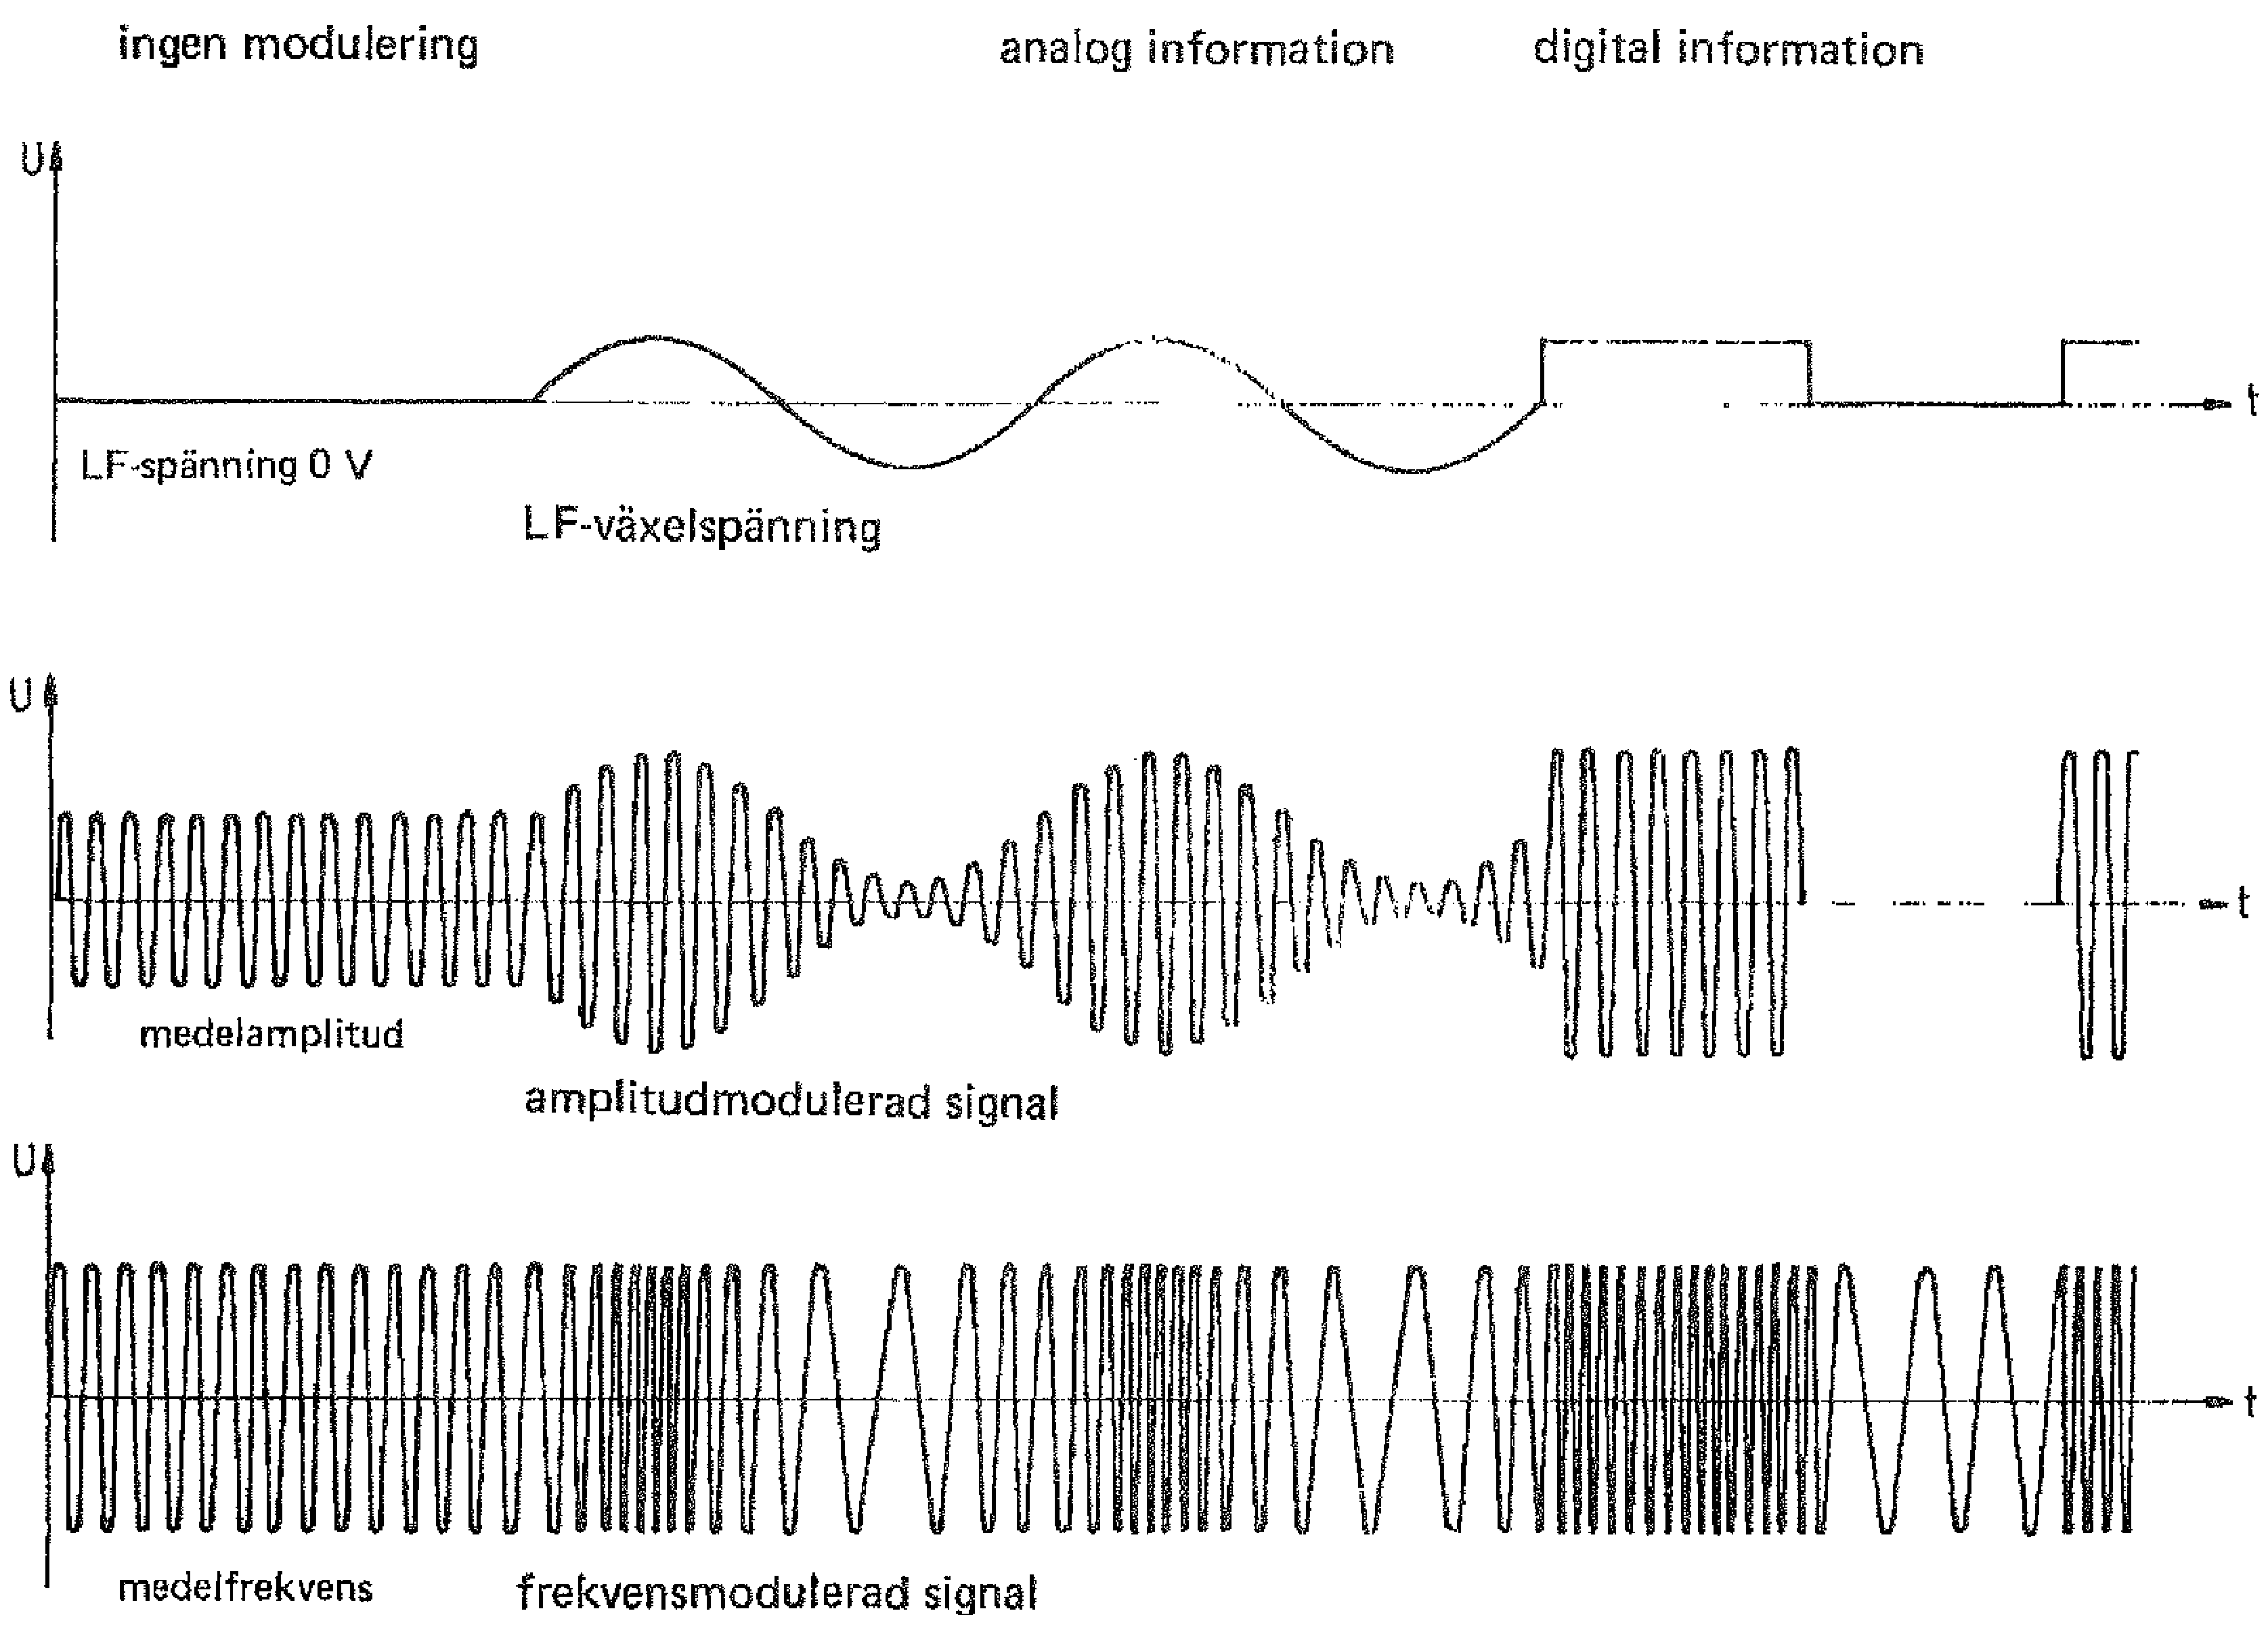
\includegraphics[width=\textwidth]{images/cropped_pdfs/bild_2_1-22.pdf}
\caption{Modulerade signaler}
\label{fig:BildII1-22}
\end{figure}

Bild \ref{fig:BildII1-22}.

En modulerad signal kännetecknas av dess amplitud, frekvens och fasläge.

Vid \emph{amplitudmodulation} påverkas huvudbärvågens amplitud, så att den i
varje tidpunkt motsvarar den modulerande signalens variation.

Vid \emph{frekvensmodulation} påverkas huvudbärvågens frekvens, så att den i
varje tidpunkt motsvarar den modulerande signalens variation.

Vid \emph{fasmodulation}, som är besläktad med frekvensmodulation, påverkas i
stället för frekvensen huvudbärvågens fasläge i förhållande till en
referenssignal, så att fasläget i varje tidpunkt motsvarar den modulerande
signalens variation.

Frekvens- och fasmodulation liknar varandra och kan sammanfattas som
vinkelmodulation, eftersom fasvinkeln mellan bärvågens spänning och ström
varierar i båda fallen.

Vid \emph{pulsmodulation} används pulståg (korta upprepade bärvågspaket); t.ex.
pulsamplitud-, pulslängds-, pulsläges- och pulskodmodulation. Pulskodmodulation
används t.ex. vid samtidig överföring av flera telesamtal på samma linje,
bärvåg etc.

\subsection{Bandbredd vid olika sändningsslag}
\textbf{HAREC a.\ref{HAREC.a.1.8.5}\label{myHAREC.a.1.8.5b}}

Varje radiosändning tar upp plats omkring den nominella bärvågsfrekvensen --
tillsammans \emph{bandbredden}.

Radioamatören måste veta detta ''platsbehov'', främst för att inte sända utanför
de frekvensband som är tilldelade för amatörradioanvändning, men även för att
kunna umgås med annan trafik inom banden.

I alla sändningsslag ökar den använda bandbredden med ökad modulation. Eftersom
största \emph{frekvenseffektivitet} alltid ska eftersträvas så upptar en
sändare med kraftigare modulation än vad som behövs för en överföring, alltid
onödigt frekvensutrymme.

\subsection{Beskrivningskod för sändningsslagen}

Vid 1979 års radioförvaltningskonferens (WARC 79) i Geneve reviderades det
internationella radioreglementet (RR), som i huvudsak trädde i kraft 1982.
Däri ingår bl.a. ett nytt system för klassindelning och beteckning av sätten
att utsända information över radio m.m. Reglementet har reviderats senare, men
i detta stycke gäller det ännu.

Indelningen i sändningsslag behövs för att känneteckna utsändningarna, t.ex. i
frekvenslistor, författningar och föreskrifter. Indelningen är också av stort
värde vid teknisk beskrivning av apparater och system för radiokommunikation.

Emellertid används av många även äldre benämningar, vilka lever kvar i
litteraturen, i märkning av manöverdonen på sändare och mottagare o.s.v.

Dessa äldre benämningar är dock inte entydiga och skapar lätt missförstånd,
varför beskrivningskoden enligt WARC 79 bör användas för tydlighetens skull.

Här följer avkortade koder enligt WARC 79 för några av de sändningsslag, som
amatörer använder mest, samt för jämförelse även de benämningar som fortfarande
används jämsides (se vidare i Appendix E).

\begin{description}
\item[NON] Bärvåg utan modulerande signal. Ingen information.

\item[A1A] Bärvåg med dubbla sidband. En enda kanal med kvantiserad bärvåg.
Ingen modulerande underbärvåg. Telegrafi.

\emph{Även kallat nycklad bärvåg (CW).}

\item[A3E] Linjärt modulerad huvudbärvåg. Dubbla sidband. En enda kanal med
analog information. Telefoni.

\emph{Även kallat amplitudmodulation (AM).}

\item[J3E] Linjärt modulerad huvudbärvåg. Ett sidband med undertryckt bärvåg.
En enda kanal med analog information. Telefoni.

\emph{Även kallat enkelt sidband (Single Side Band -- SSB).}

\item[F3E] Vinkelmodulerad bärvåg. Frekvensmodulering. En enda kanal med analog
information. Telefoni.

\emph{Även kallat frekvensmodulering (FM).}

\item[G3E] Vinkelmodulerad bärvåg. Fasmodulering. En enda kanal med analog
information. Telefoni.

\emph{Även kallat fasmodulering (PM).}
\end{description}

Såväl A1A, A3E som J3E är sändningsslag där amplituden moduleras. Därför är
termen \emph{amplitudmodulation} inte tillräcklig för att beskriva flera
likartade sändningsslag.

\subsection{Modulerande signaler}
\textbf{HAREC a.\ref{HAREC.a.1.7.1}\label{myHAREC.a.1.7.1}}
\index{modulerande signaler}

\subsubsection{Basband}
\index{basband}

Basband är ett frekvensområde för en modulerande signal. Det finns ett basband
för alla slags modulerande signaler, vare sig de är analoga eller digitala. Det
kan finnas mer än ett basband i en komplett modulationsprocess. Till exempel är
en nycklad ton, som går till sändaren genom mikrofoningången, dess analoga
basband medan nycklingspulserna till tongeneratorn är dess digitala basband.

\begin{figure}
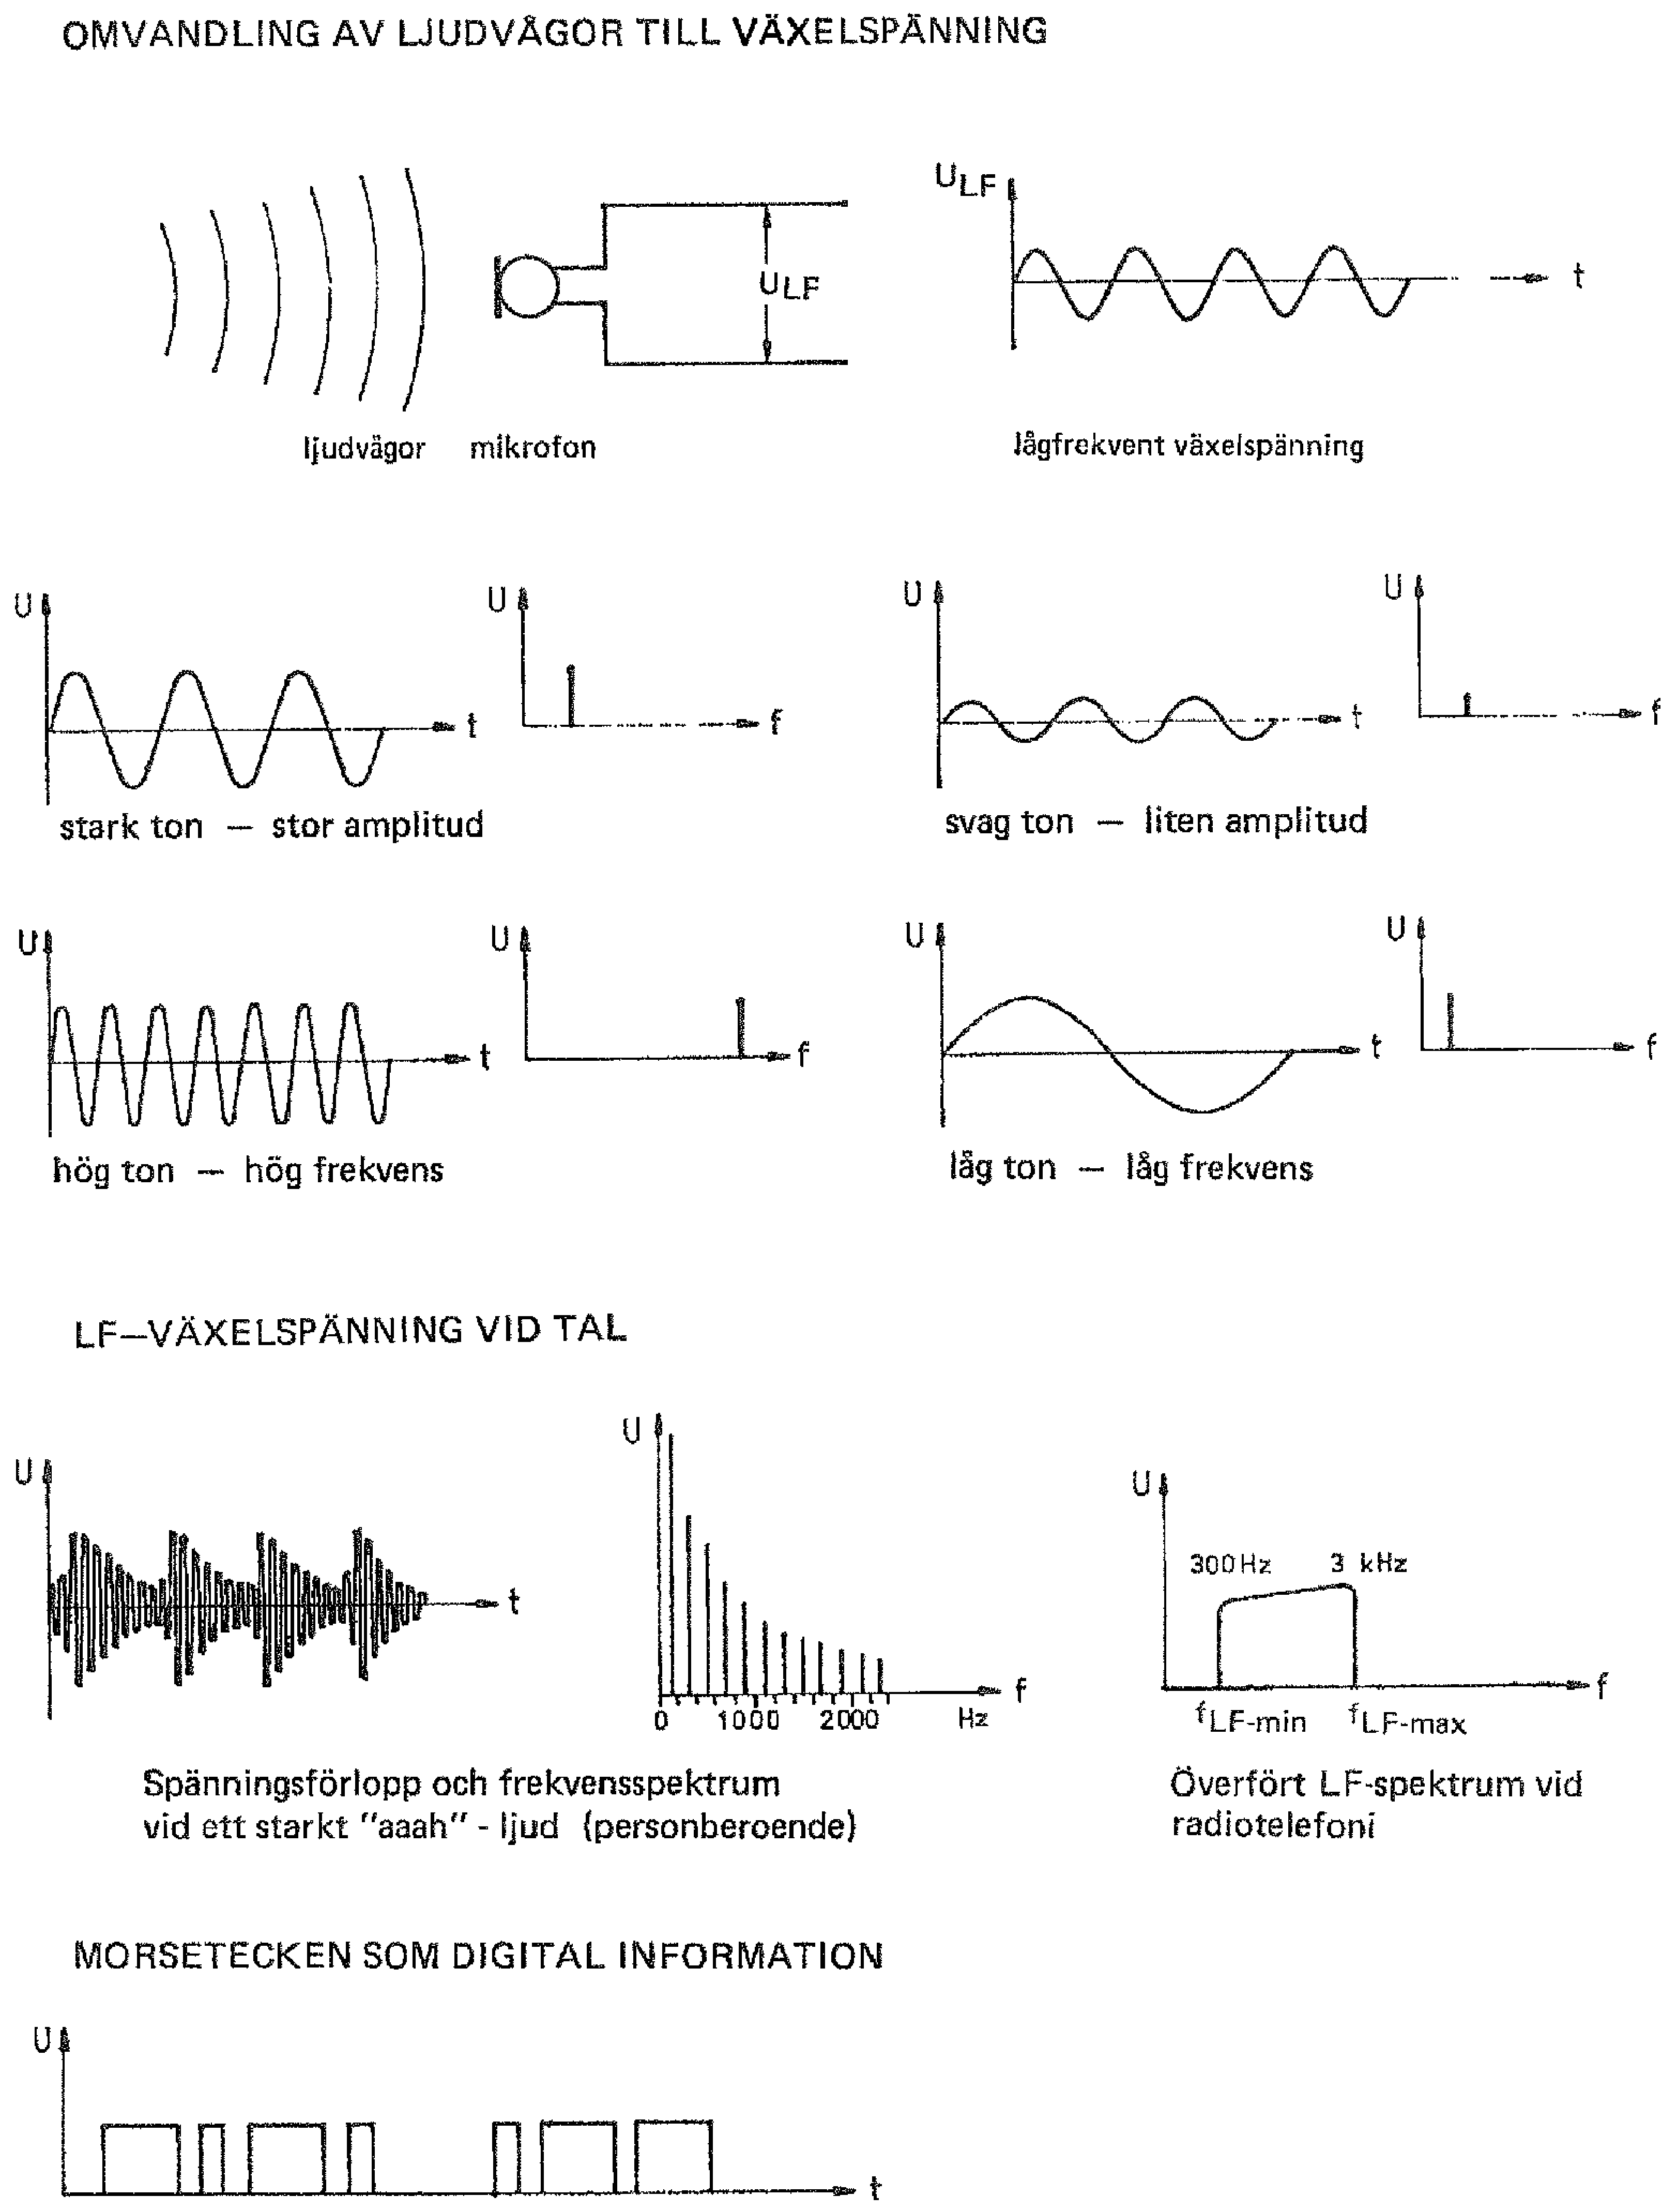
\includegraphics[width=\textwidth]{images/cropped_pdfs/bild_2_1-23.pdf}
\caption{Modulerande signaler}
\label{fig:BildII1-23}
\end{figure}

Bild \ref{fig:BildII1-23}.

Ett vanligt sätt att överföra information över radio är med telefoni, d.v.s.
tal.

Frekvensområdet 300--3000~Hz räcker för god förståelighet av tal. Dels är örat
känsligast inom det området och dels finns där den mesta energin i talet.

Mikrofonen tar upp de lufttrycksvariationer, som uppstår när man talar, och
omvandlar dem till elektriska svängningar. Svängningarna varierar mellan
positiva och negativa spänningsvärden.

\subsubsection{Försök}

\begin{enumerate}
\item Anslut en mikrofon till ett oscilloskop och studera spänningsförloppen
för olika slags ljud, toner, tal osv. som funktion av tiden. På bilden är
dessa svängningar mycket förenklade, t.ex. sinusformade.

\item Anslut en högtalare och ett oscilloskop till en LF-generator, vars
frekvens och amplitud kan ändras. Lyssna på ljud med låg och hög frekvens samt
på svaga och starka ljud. En baston har låg frekvens och en diskantton har hög
frekvens. En svag ton har liten amplitud och en stark ton har stor amplitud.
\end{enumerate}

\subsection{Sändningsslaget A3E (även kallat AM)}
\textbf{HAREC a.\ref{HAREC.a.1.8.2}, a.\ref{HAREC.a.1.8.6b}, a.\ref{HAREC.a.1.8.7b}\label{myHAREC.a.1.8.2}\label{myHAREC.a.1.8.6b}\label{myHAREC.a.1.8.7b}}
\index{amplitudmodulation}
\index{A3E}
\index{AM}

\begin{figure}
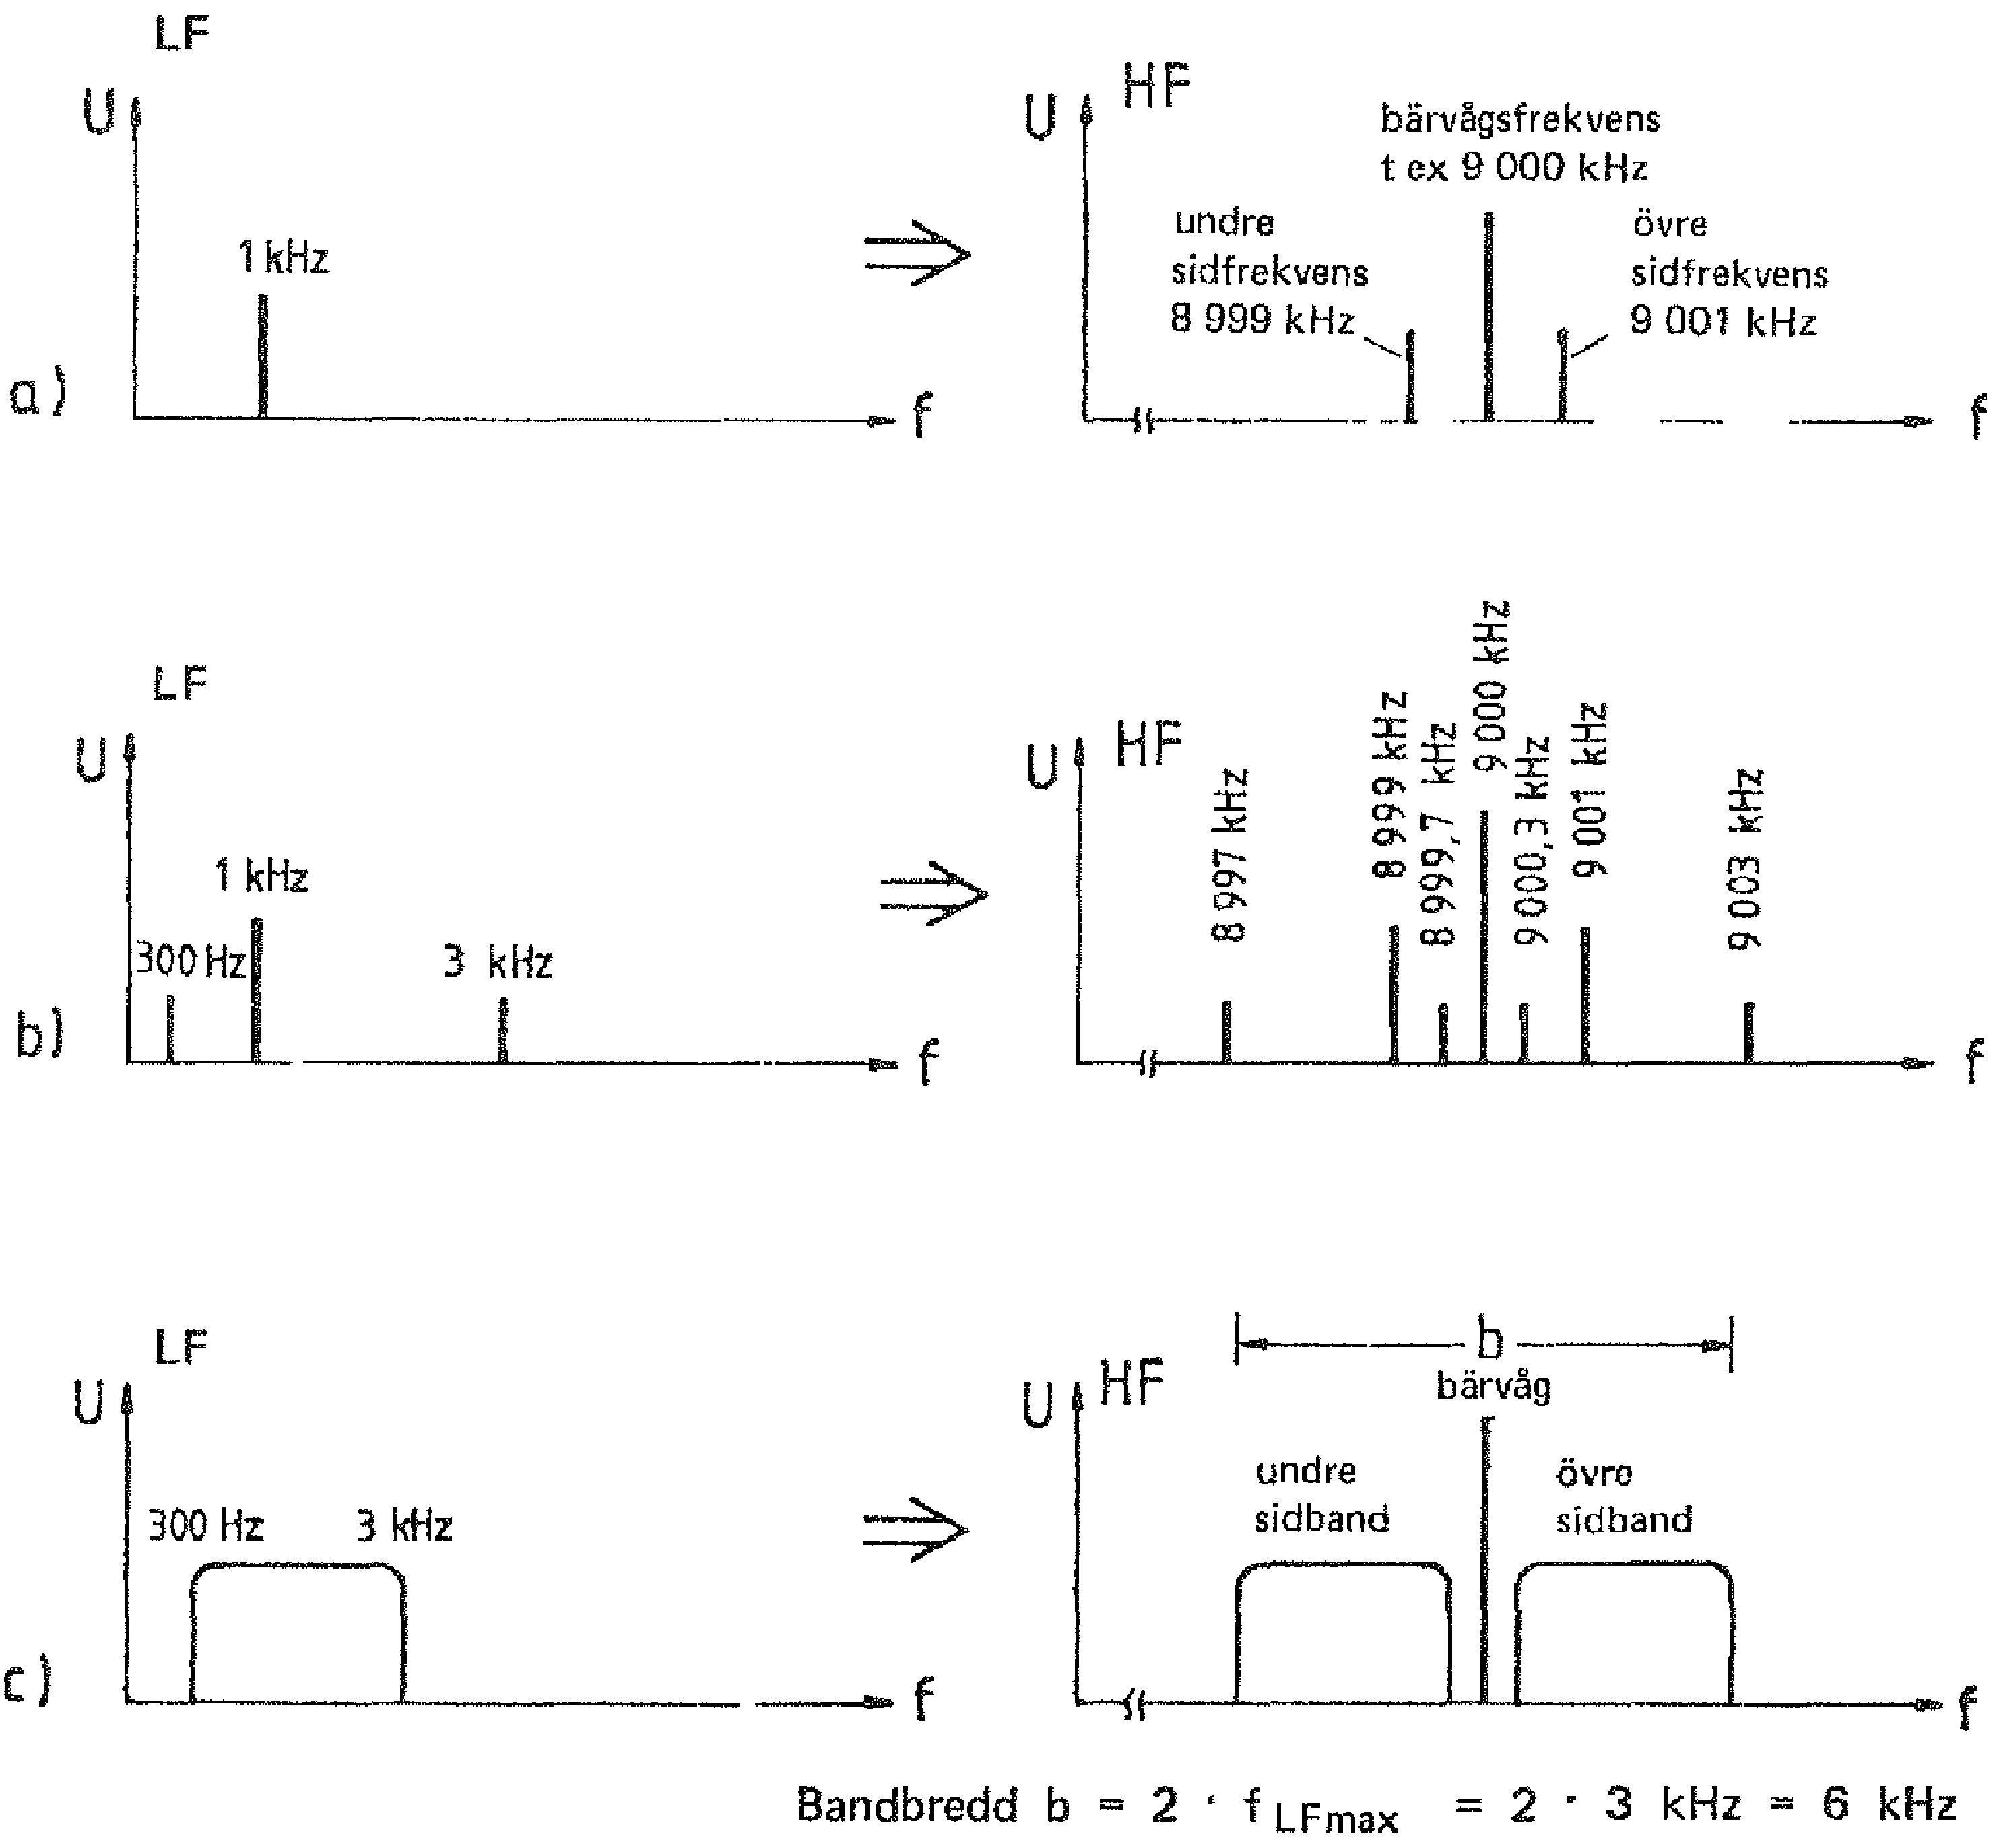
\includegraphics[width=\textwidth]{images/cropped_pdfs/bild_2_1-24.pdf}
\caption{Sidband vid A3E-modulation}
\label{fig:BildII1-24}
\end{figure}

Bild \ref{fig:BildII1-24}.

Bilden visar frekvensspektrum av en signal vid amplitudmodulation med

\begin{enumerate}[label=\alph*.,noitemsep]
\item en sinuston,
\item en blandning av tre sinustoner,
\item ett frekvensspektrum.
\end{enumerate}

\subsubsection{Försök}

Modulera en A3E-sändare med en 3~kHz signal. Med en mottagare utrustad med ett
smalt filter för telegrafi, kan man urskilja och påvisa bärvågen och de båda
sidbanden.

\subsubsection{A3E-modulation med en ton}

\begin{figure}
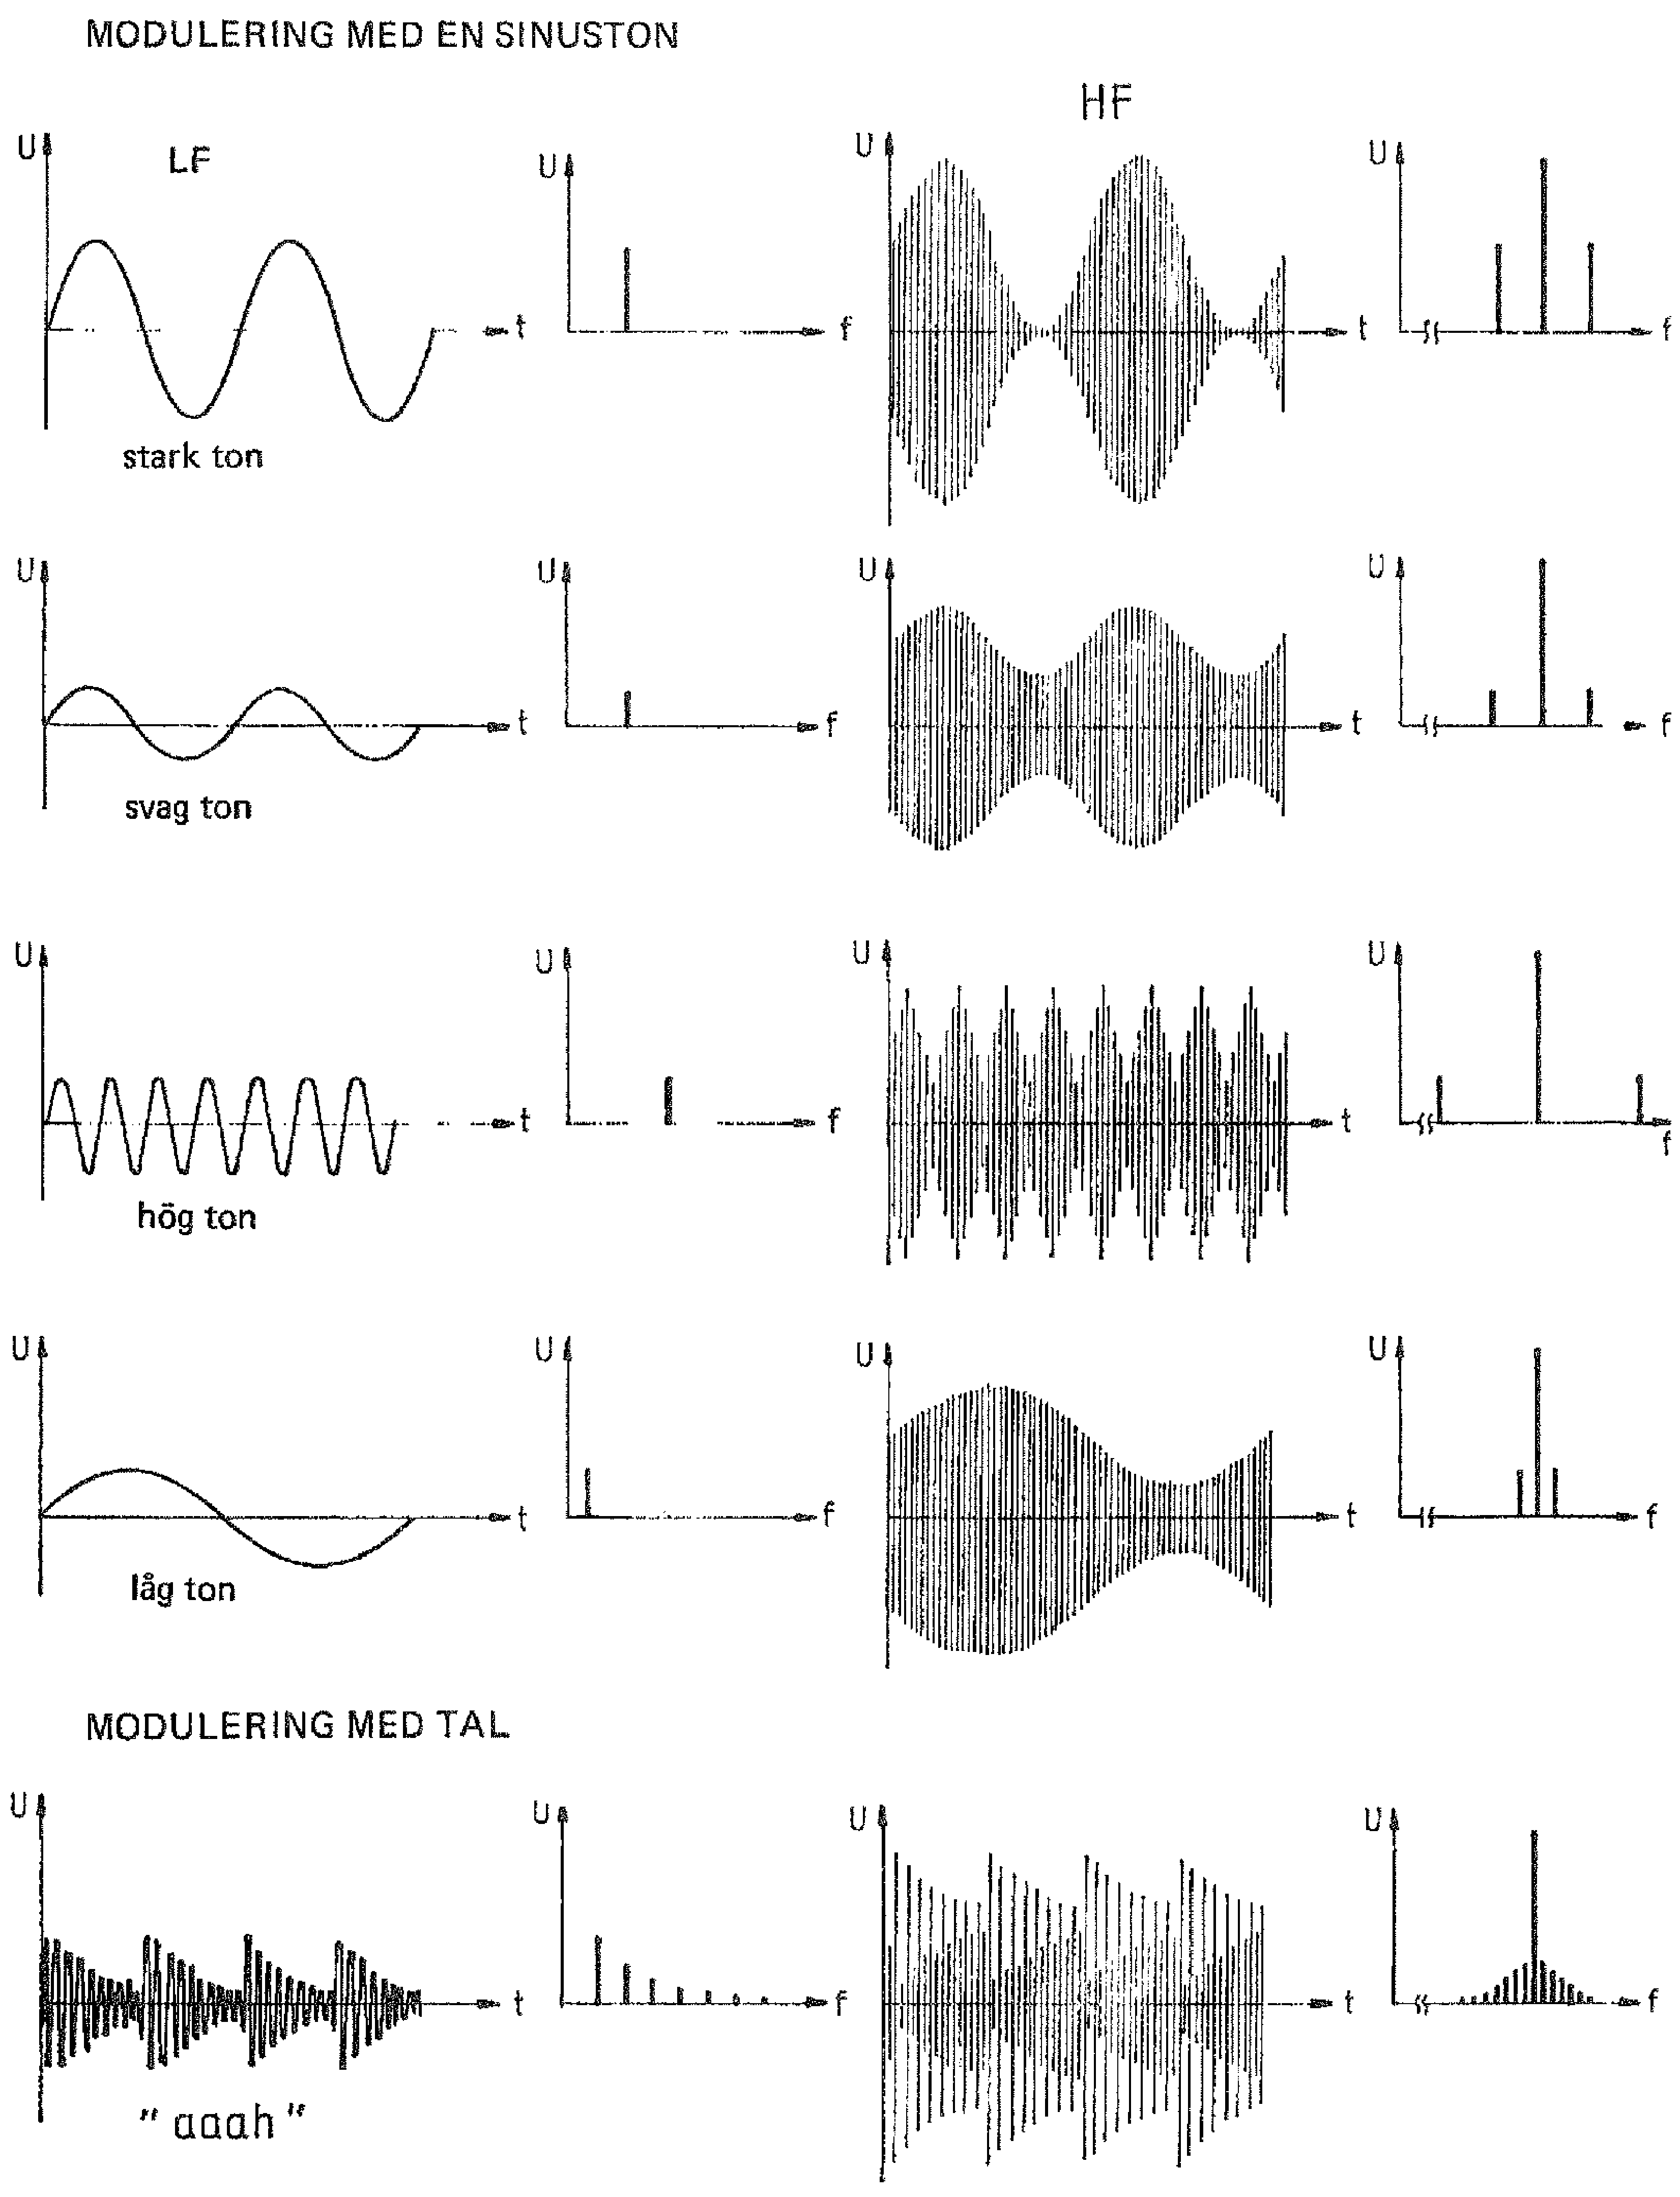
\includegraphics[width=\textwidth]{images/cropped_pdfs/bild_2_1-25.pdf}
\caption{A3E-modulation med toner med olika styrka och frekvens}
\label{fig:BildII1-25}
\end{figure}

Bild \ref{fig:BildII1-25}.

En omodulerad bärvåg har konstant amplitud. En amplitudmodulerad signal är i
grunden resultatet av svävning mellan frekvenser eller av icke linjär blandning
av frekvenser. När bärvåg och basband blandas, så är särskilt tre
blandningsprodukter av intresse.

Dessa är

\begin{enumerate}[label=-,noitemsep]
\item bärvågen,
\item det lägre sidbandet (förkortat LSB) och
\item det övre sidbandet (förkortat USB).
\end{enumerate}

AM-signalen består således inte bara av bärvågsfrekvensen \(f_{HF}\) utan även
av övre och nedre sidofrekvenser, vilka är summan och skillnaden av
bärvågsfrekvensen \(f_{HF}\) och den modulerande frekvensen \(f_{LF}\).
Alltså \(f_{HF} + f_{LF}\) (övre sidofrekvens) och skillnadsfrekvensen
\(f_{HF} - f_{LF}\) (undre sidofrekvens).

Eftersom tal inte bara omfattar en enda frekvens utan ett helt frekvensspektrum
(ca 0,3--3~kHz), så uppstår inte bara två sidofrekvenser utan två sidband, det
lägre sidbandet (LSB, Lower Side Band) och det övre (USB, Upper Side Band).

LF-signalens frekvens bestämmer sidofrekvensens avstånd från bärvågen.
Bandbredden på en amplitudmodulerad signal med full bärvåg och två sidband är
dubbelt så stor som den högsta modulerande LF-frekvensen:

\(b= 2 \cdot f_{LFmax}\)

Om de modulerande LF-frekvenserna är mellan 0,3 och 3~kHz, så blir sändningens
totala bandbredd 6~kHz.

LF-signalernas amplitud påverkar sidbandens och sidofrekvensernas amplitud. Vid
maximal modulation (100~\% modulationsgrad) varierar signalamplituden mellan
noll och dubbla värdet av det för en omodulerad bärvåg.

Som mest kan vardera sidbandet överföra en fjärdedel så mycket effekt som
bärvågen, d.v.s. en sjättedel av den totalt utsända effekten. Då avger sändaren
dubbelt så stor medeleffekt som utan modulation. Toppeffekten (PEP,
Peak Envelope Power) är till och med fyra gånger så stor.

Slutförstärkaren och kraftförsörjningen måste dimensioneras för toppeffekten vid
full modulation eller att modulationsgraden anpassas så att överbelastning inte
sker.

\subsubsection{Fördelar med A3E-modulation}

En A3E-sändare är enkel jämfört med en J3E-sändare, vilken har en mer
komplicerad signalbehandling.

\subsubsection{Nackdelar med A3E-modulation}

Eftersom samma information finns i båda sidbanden och ingen finns i bärvågen,
så sänds effekten i bärvågen och ett av sidbanden ut till ingen nytta. I
talpauser sänds endast bärvågseffekten och till ingen nytta. Även
frekvensutrymme slösas bort. Då en annan, alltför närliggande sändares bärvåg
blandas med den egna, så alstras interferenstoner i mottagarna.

\subsection{Sändningsslaget A1A (även kallat CW)}
\textbf{HAREC a.\ref{HAREC.a.1.8.1}, a.\ref{HAREC.a.1.8.6a}, a.\ref{HAREC.a.1.8.7a}\label{myHAREC.a.1.8.1}\label{myHAREC.a.1.8.6a}\label{myHAREC.a.1.8.7a}}
\index{A1A}
\index{CW}

\begin{figure}
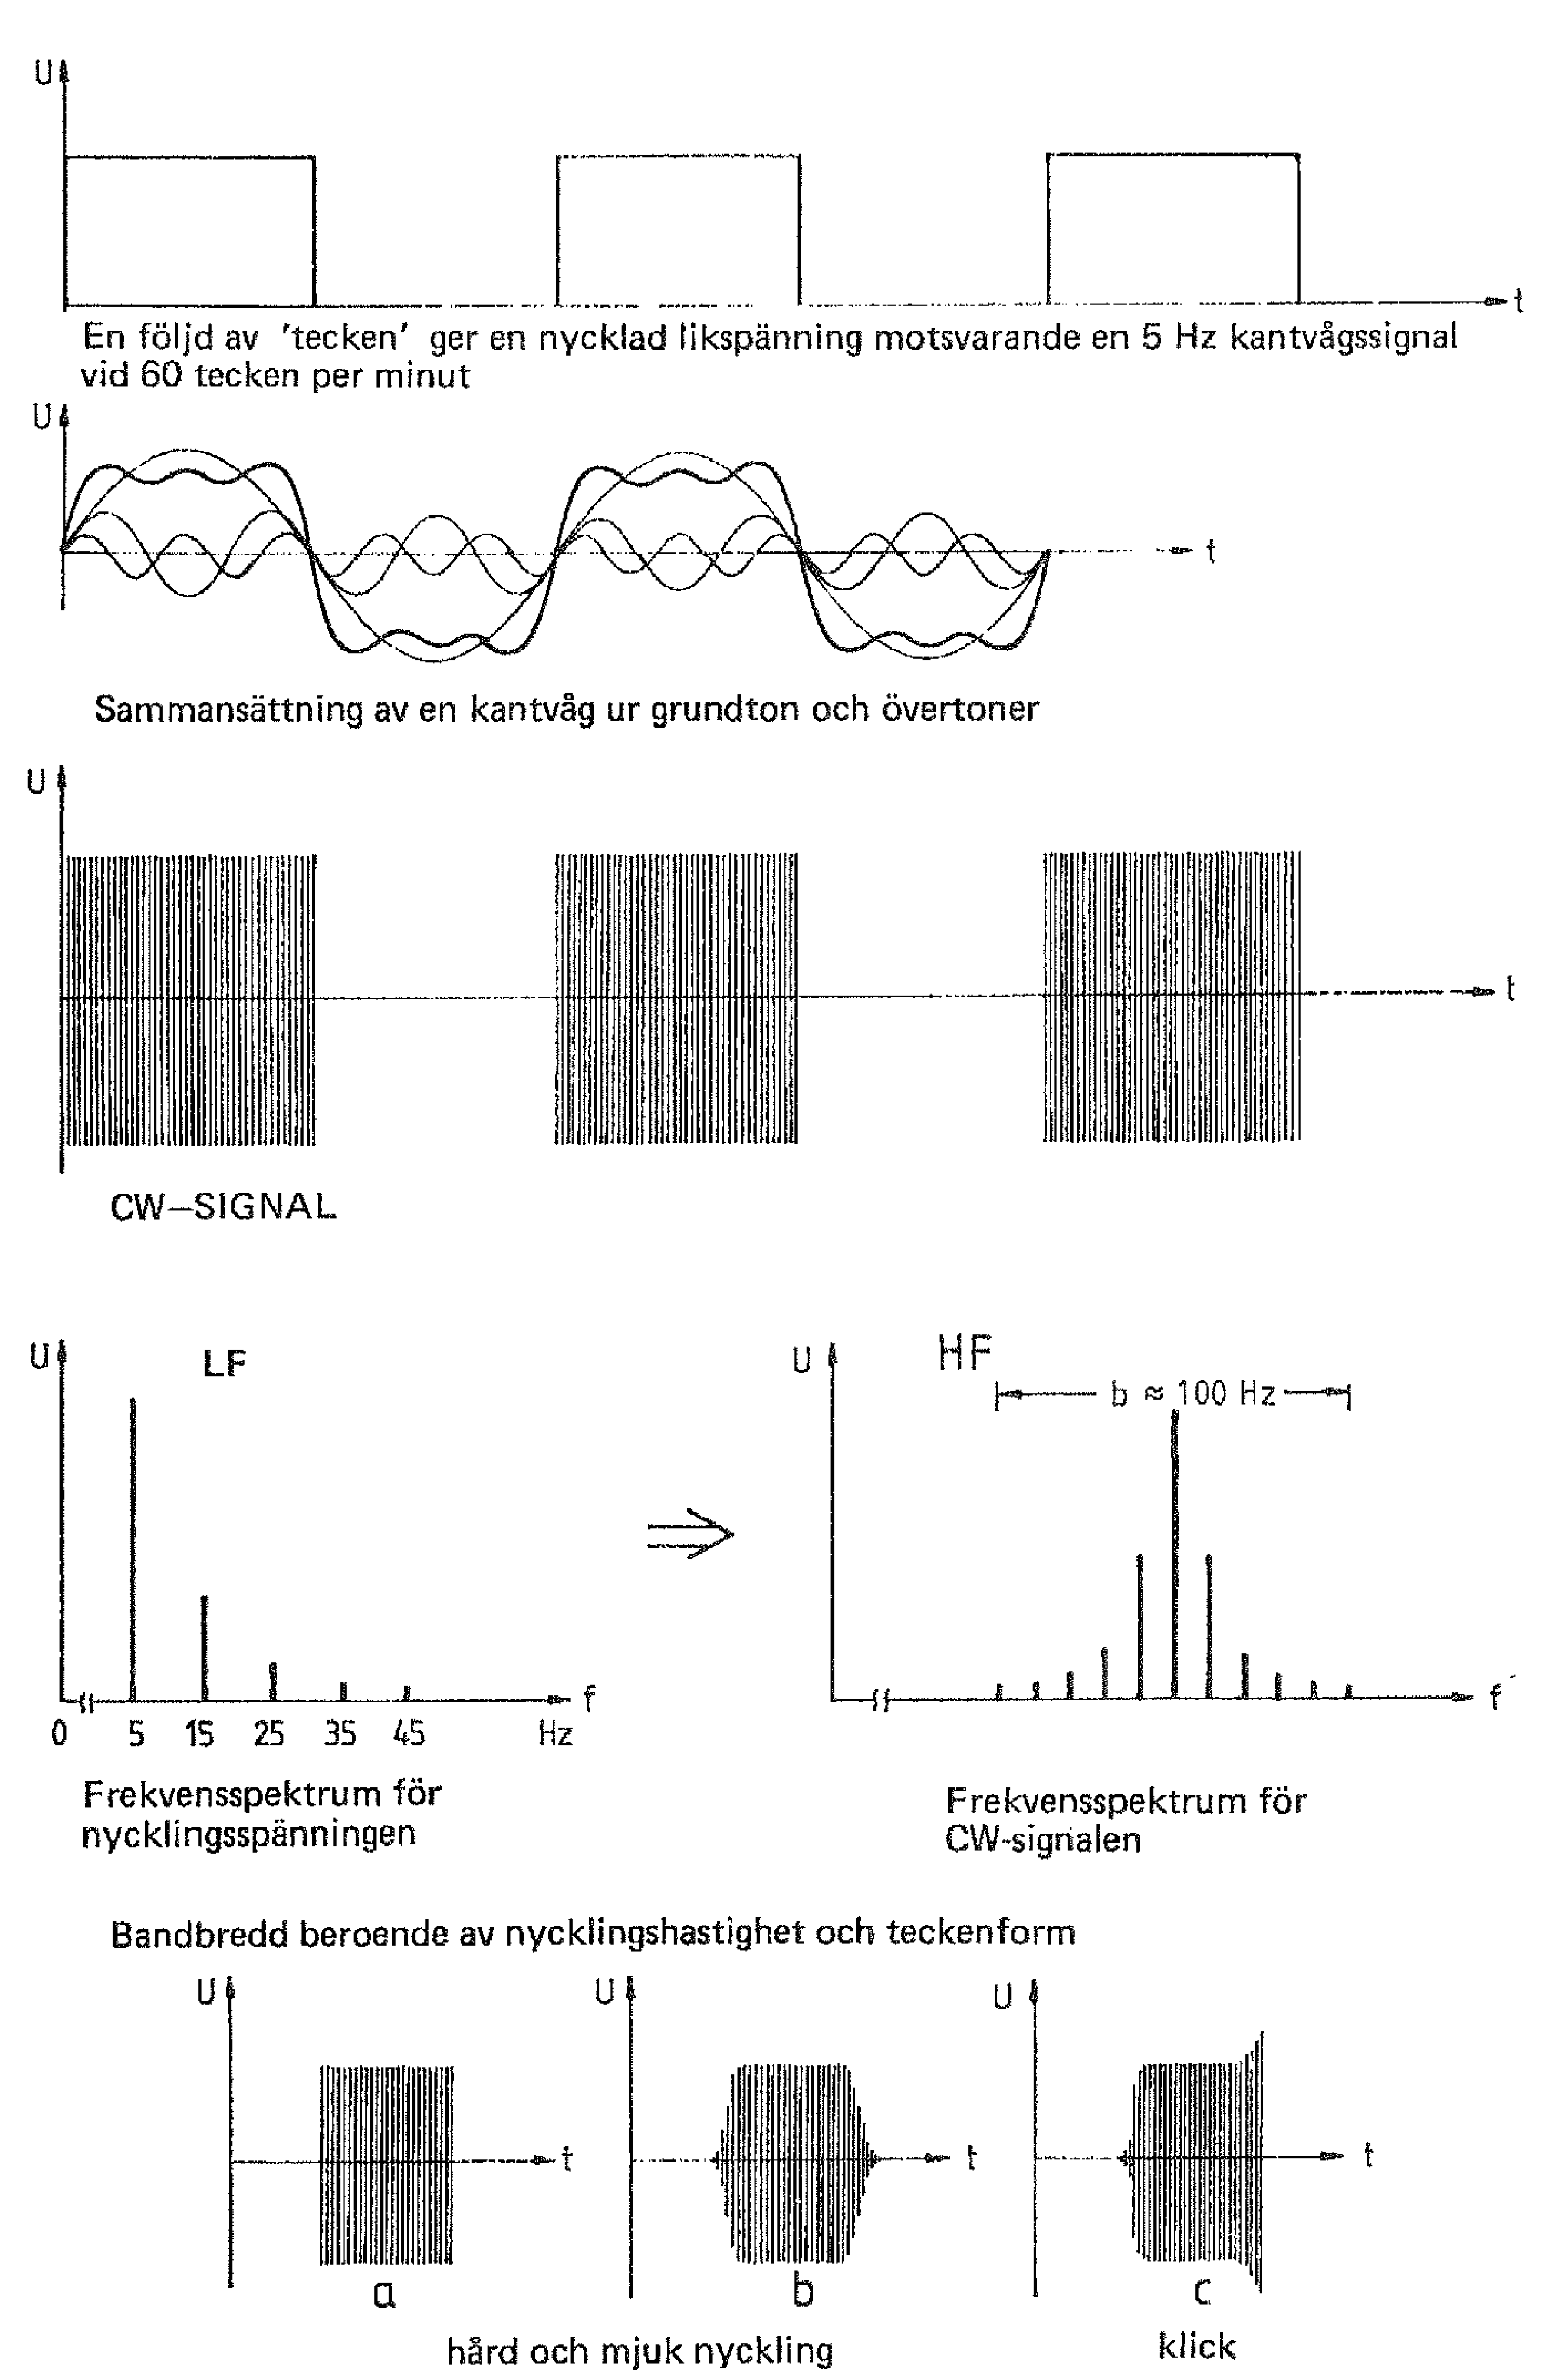
\includegraphics[width=\textwidth]{images/cropped_pdfs/bild_2_1-26.pdf}
\caption{Amplitudmodulation med morsetecken}
\label{fig:BildII1-26}
\end{figure}

Bild \ref{fig:BildII1-26}.

Man kan överföra meddelanden med morsetelegrafi på olika sätt. Det enklaste
sättet är att koppla in och ur sändarens bärvåg i takt med teckendelarna i
morsetecknen. Man kan kalla det för bärvågstelegrafi. Förfarandet kallas sedan
mycket länge även för CW (continous waves), vilket egentligen anger att
bärvågen svänger med konstant amplitud, om man bortser från att den nycklas.
Detta i motsats till de dämpade bärvågssvängningar som var fallet i sedan
mycket länge förbjudna s.k. gnistsändare.

Fastän en sändare ''moduleras utan ton'', har den en viss bandbredd. Det beror på
att den takt, som sändaren nycklas med, egentligen är en ton -- låt vara med låg
frekvens. Antag att sändaren nycklas med en serie korta morsetecken. Vid
telegraferingshastigheten 60 tecken/minut alstrar bärvågspulserna en kantvåg
med frekvensen 5~Hz. Som tidigare beskrivits, består en sådan kantvåg av summan
av sinussignaler med frekvenserna 5~Hz, 15~Hz, 25~Hz, 35~Hz o.s.v.

Det innebär att det uppstår sidofrekvenser över och under bärvågens frekvens och
med ett avstånd till bärvågen av 5~Hz, 15~Hz, 25~Hz, 35~Hz o.s.v.
Telegrafisändaren har alltså liksom vid A3E en bandbredd, som dels står i
förhållande till nycklingshastigheten och dels till ''kantigheten'' på tecknen,
vilket bestämmer övertonshalten i bärvågen. Vid s.k. mjuk nyckling kan den 9:e
övertonen antas vara den högsta som uppfattas av en motstation. Med en
nycklingsfrekvens av 5~Hz blir bandbredden inte större än
\(2 \cdot 10 \cdot 5 = 100\ Hz\).

En hård (kantig) och snabb teckengivning ökar bandbredden och kan resultera i
att s.k. nycklingsknäppar kan uppfattas långt vid sidan om sändningsfrekvensen.
Ju hårdare nycklingen är, desto längre bort från bärvågsfrekvensen hörs
nycklingsknäpparna. Detta stör andra stationer.

Kännetecken för sändningsslaget A1A, telegrafi genom nycklad bärvåg:

Mycket liten bandbredd, extremt gott utnyttjande av sändareffekten, stor
överföringssäkerhet, lång räckvidd, enkla sändare.

\subsection{Sändningsslaget J3E (även kallat SSB)}
\textbf{HAREC a.\ref{HAREC.a.1.8.3c}, a.\ref{HAREC.a.1.8.6c}, a.\ref{HAREC.a.1.8.7c}\label{myHAREC.a.1.8.3c}\label{myHAREC.a.1.8.6c}\label{myHAREC.a.1.8.7c}}
\index{single side band}
\index{J3E}
\index{SSB}

\subsubsection{Princip}

Som sagts är det onödigt sända ut två sidband, eftersom båda innehåller samma
information.

Signaler med endast ett sidband och undertryckt bärvåg kan alstras på flera
sätt. Numera är den s.k. filtermetoden i särklass vanligast och den enda som
behandlas här.

\begin{figure}
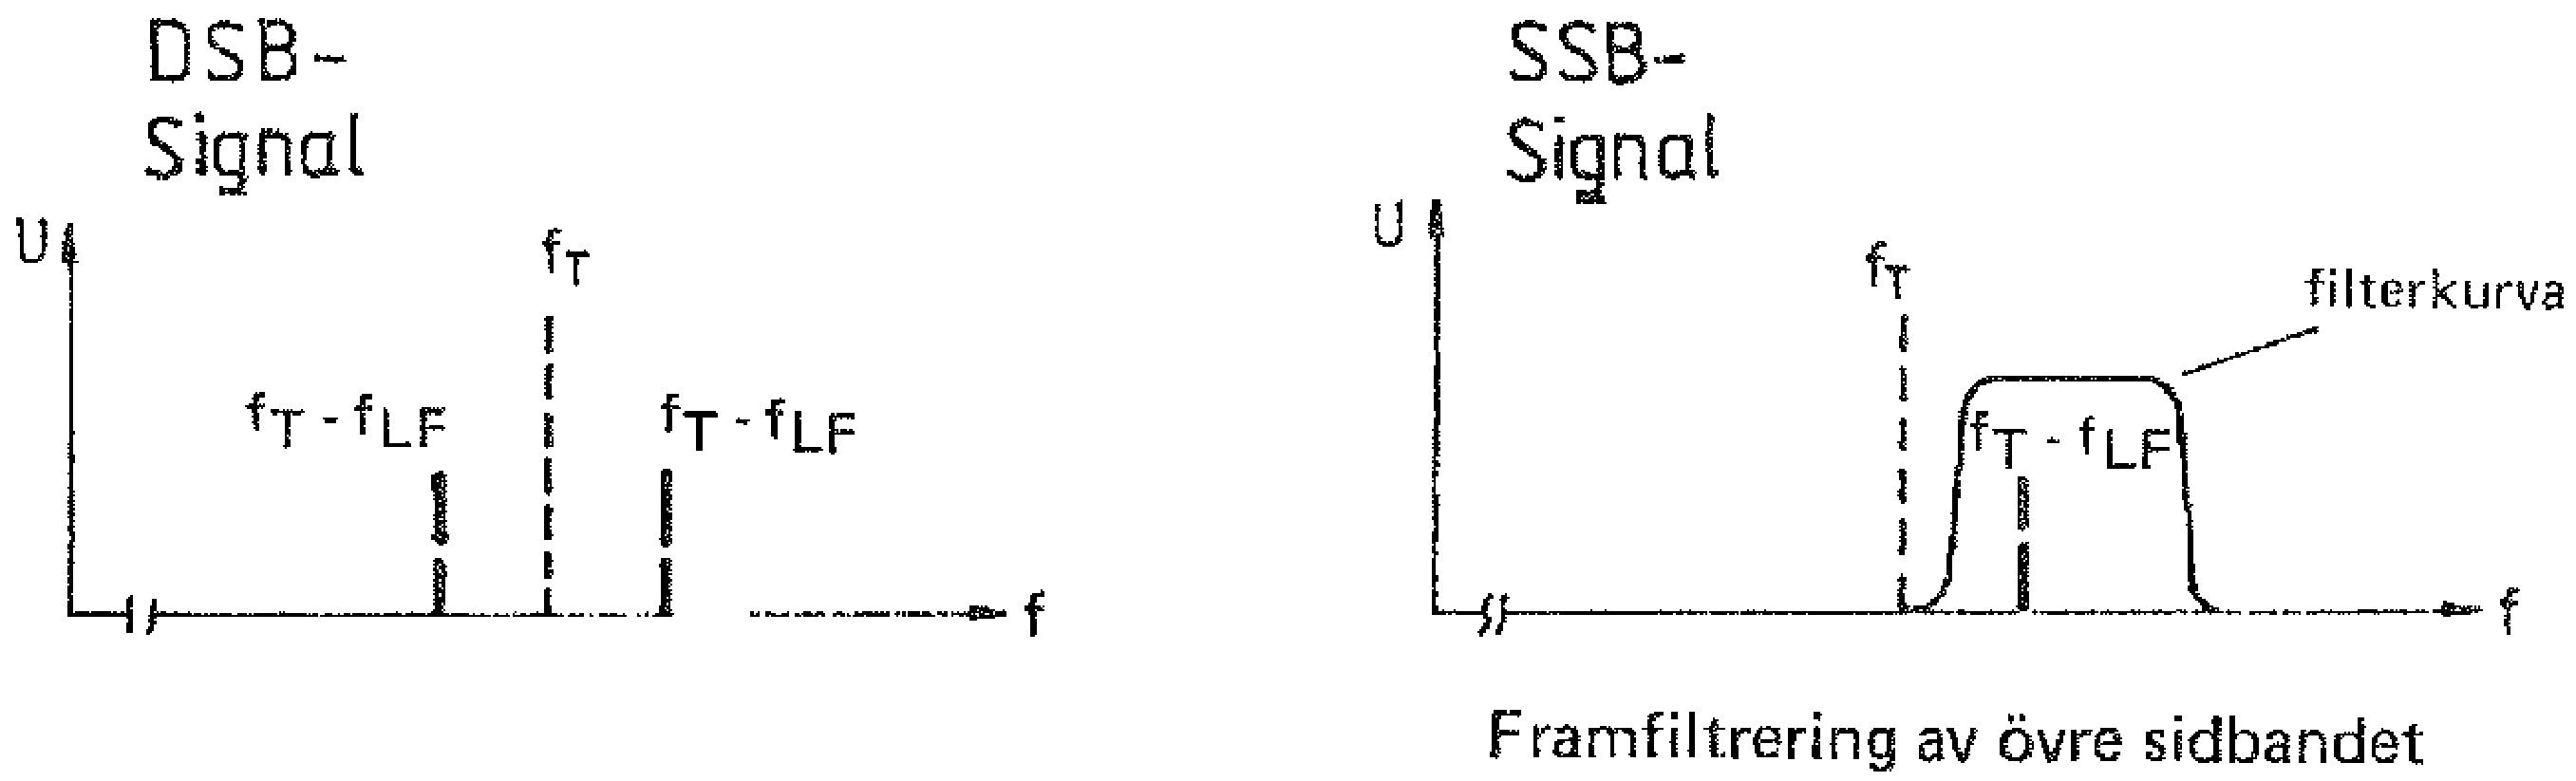
\includegraphics[width=\textwidth]{images/cropped_pdfs/bild_2_1-27.pdf}
\caption{Sidband vid DSB}
\label{fig:BildII1-27}
\end{figure}

Bild \ref{fig:BildII1-27}.

Med filtermetoden blandas HF- och LF-signalerna i en speciell blandare. Där
undertrycks båda dessa signaler medan blandningsprodukterna med deras summa-
och skillnadsfrekvenser blir kvar, d.v.s. det övre och nedre sidbandet.

Utsignalen från blandaren benämns DSB-signal (Double Side Band). Till skillnad
från i A3E-signalen saknas dock bärvågen i DSB-signalen. För att även
undertrycka det ena sidbandet före sändningen, så följs blandaren av ett
bandpassfilter med bandbredd och frekvensläge för avsett sidband.

Den signal som sänds ut innehåller därför endast ett sidband (Single Side Band).

\paragraph{Exempel}

\begin{figure}
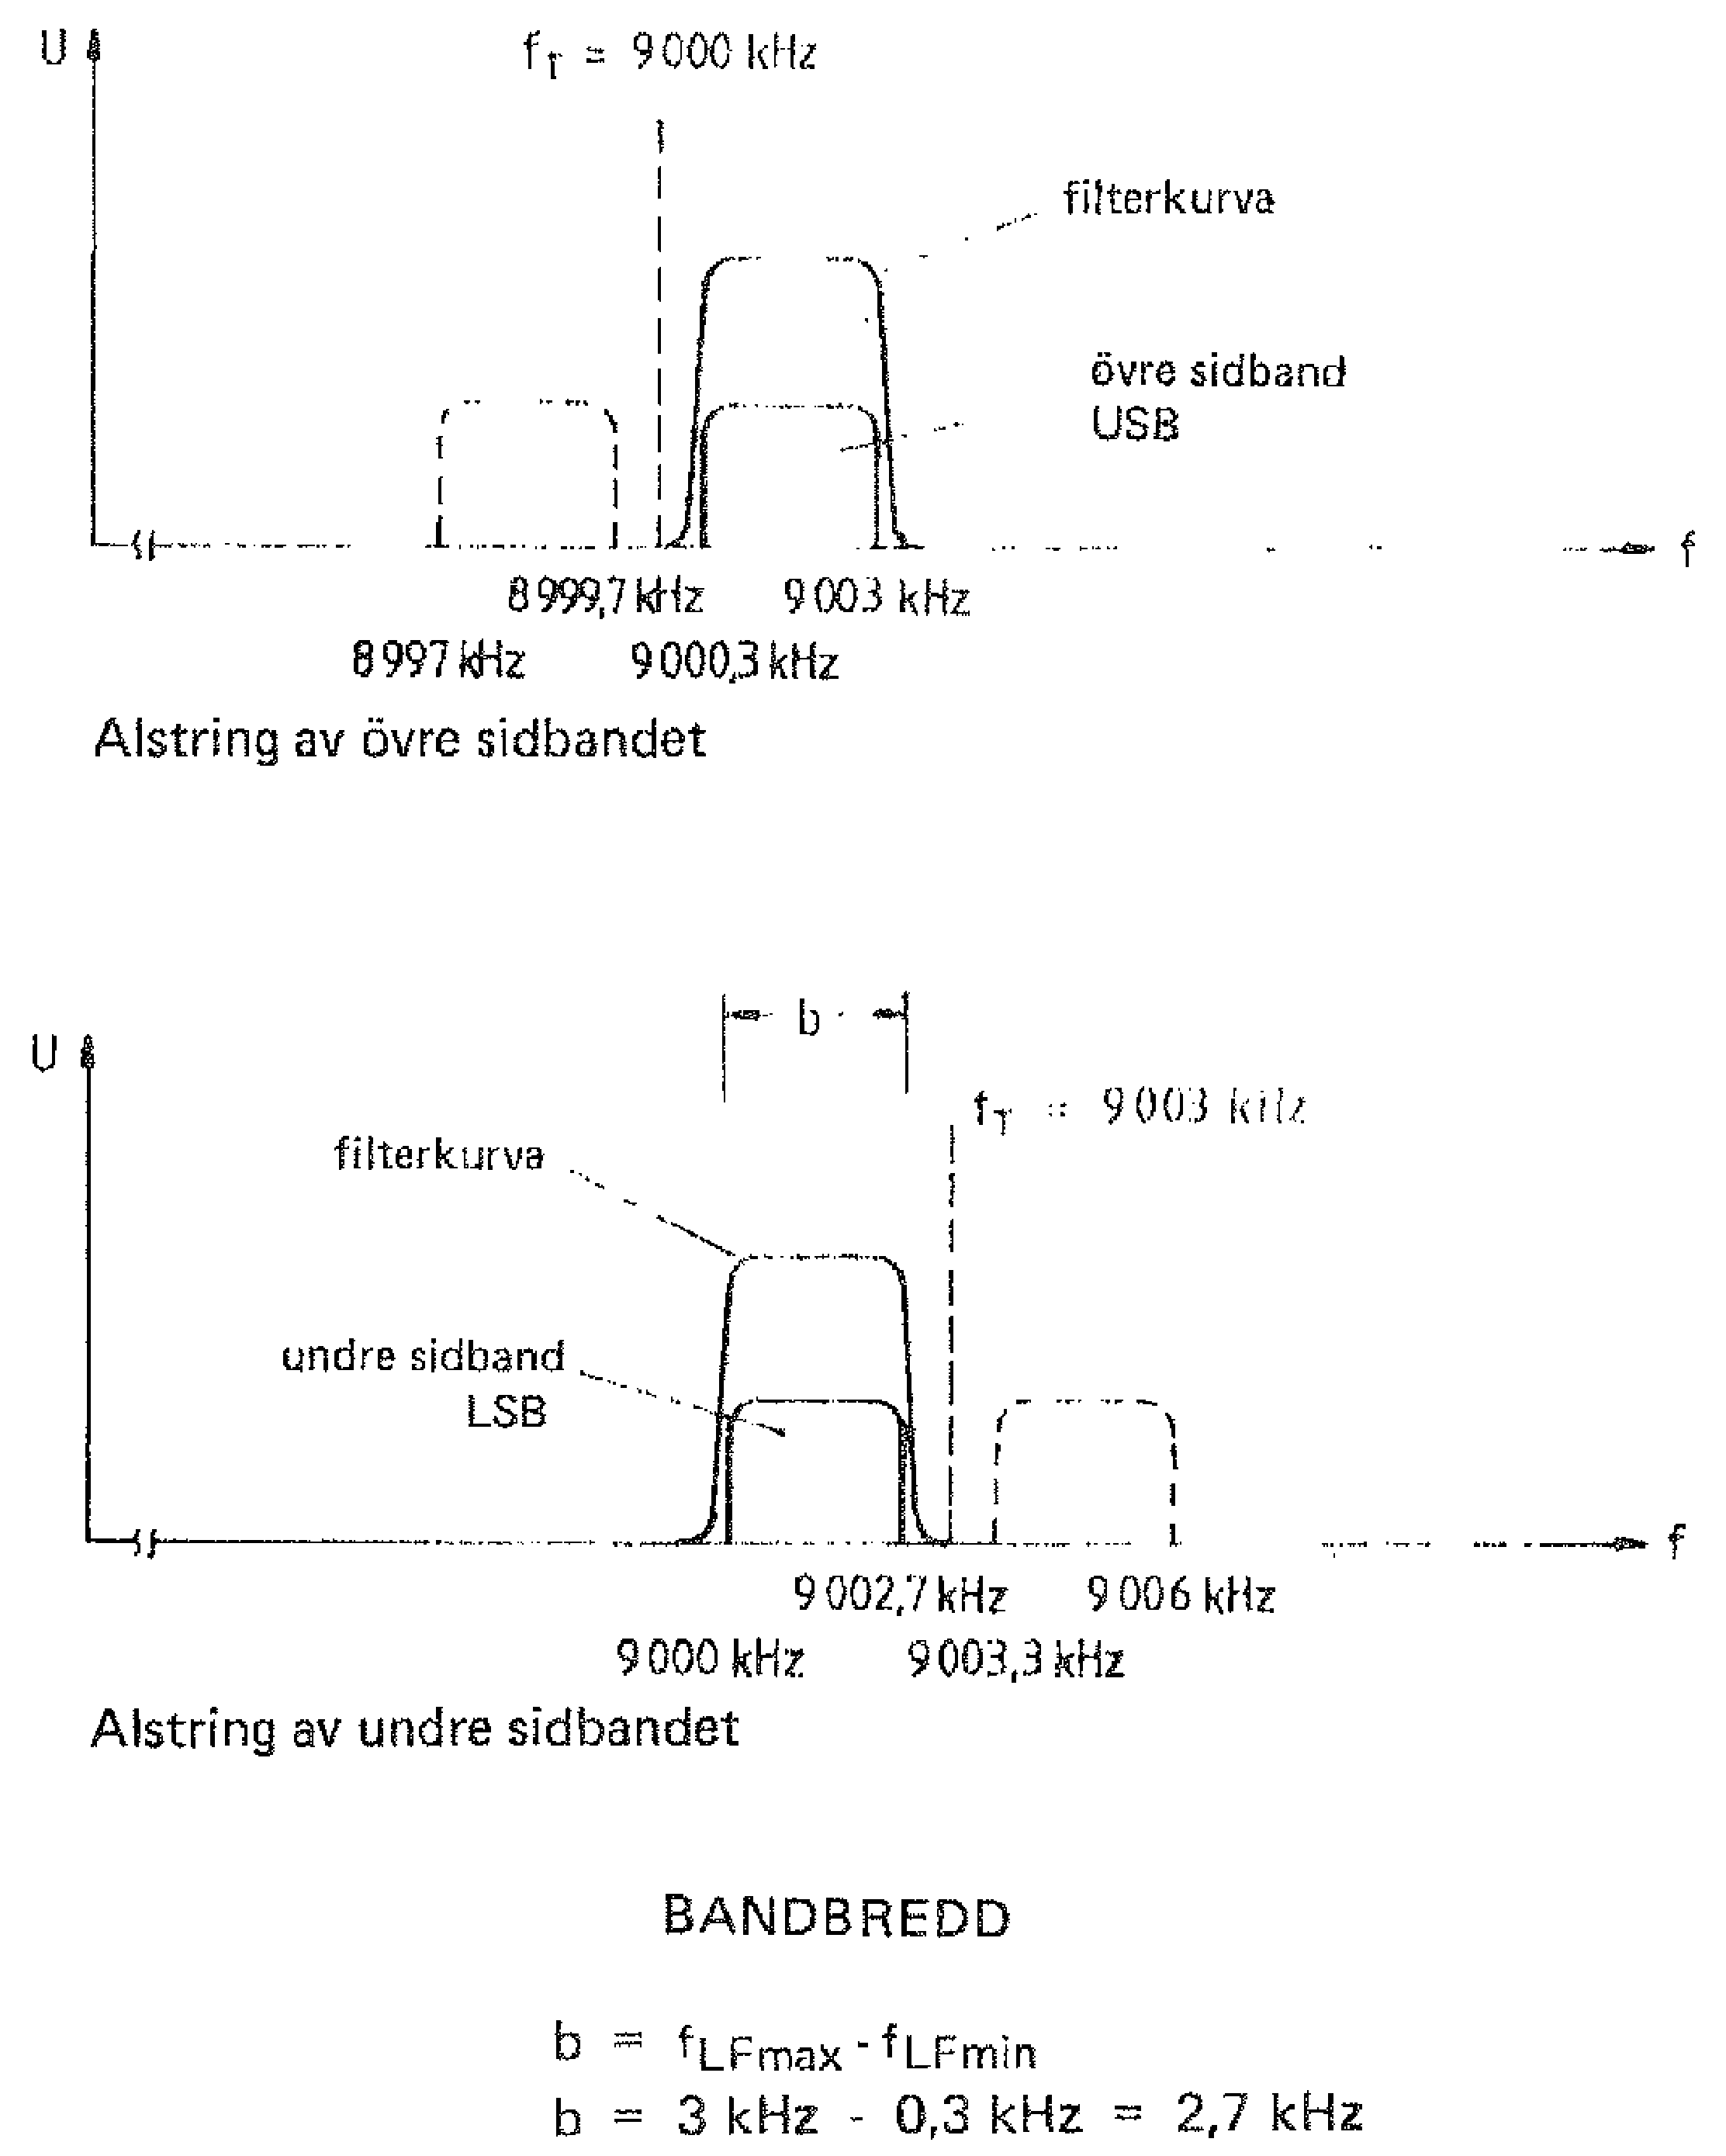
\includegraphics[width=\textwidth]{images/cropped_pdfs/bild_2_1-28.pdf}
\caption{Sidbandsval vid SSB}
\label{fig:BildII1-28}
\end{figure}

Bild \ref{fig:BildII1-28}.

Ett SSB-filter har ett passband av 9000,3--9003~kHz. Vid bärvågsfrekvensen 9000~kHz
sträcker sig det övre sidbandet från 9000,3--9003~kHz och släpps igenom. Däremot
blir bärvågsfrekvensen undertryckt.

Det undre sidbandet 8997--8999,7~kHz faller utanför filtrets passband och blir
också undertryckt.

Ska däremot det undre sidbandet kunna passera igenom samma filter, så måste
bärvågsfrekvensen höjas med 3~kHz, alltså till 9003~kHz. Då faller det undre
sidbandet, 9002,7--9000,0~kHz inom filtrets passband.

Det övre sidbandet 9003,3--9006,0~kHz faller nu utanför passbandet och blir
undertryckt.

\begin{figure}
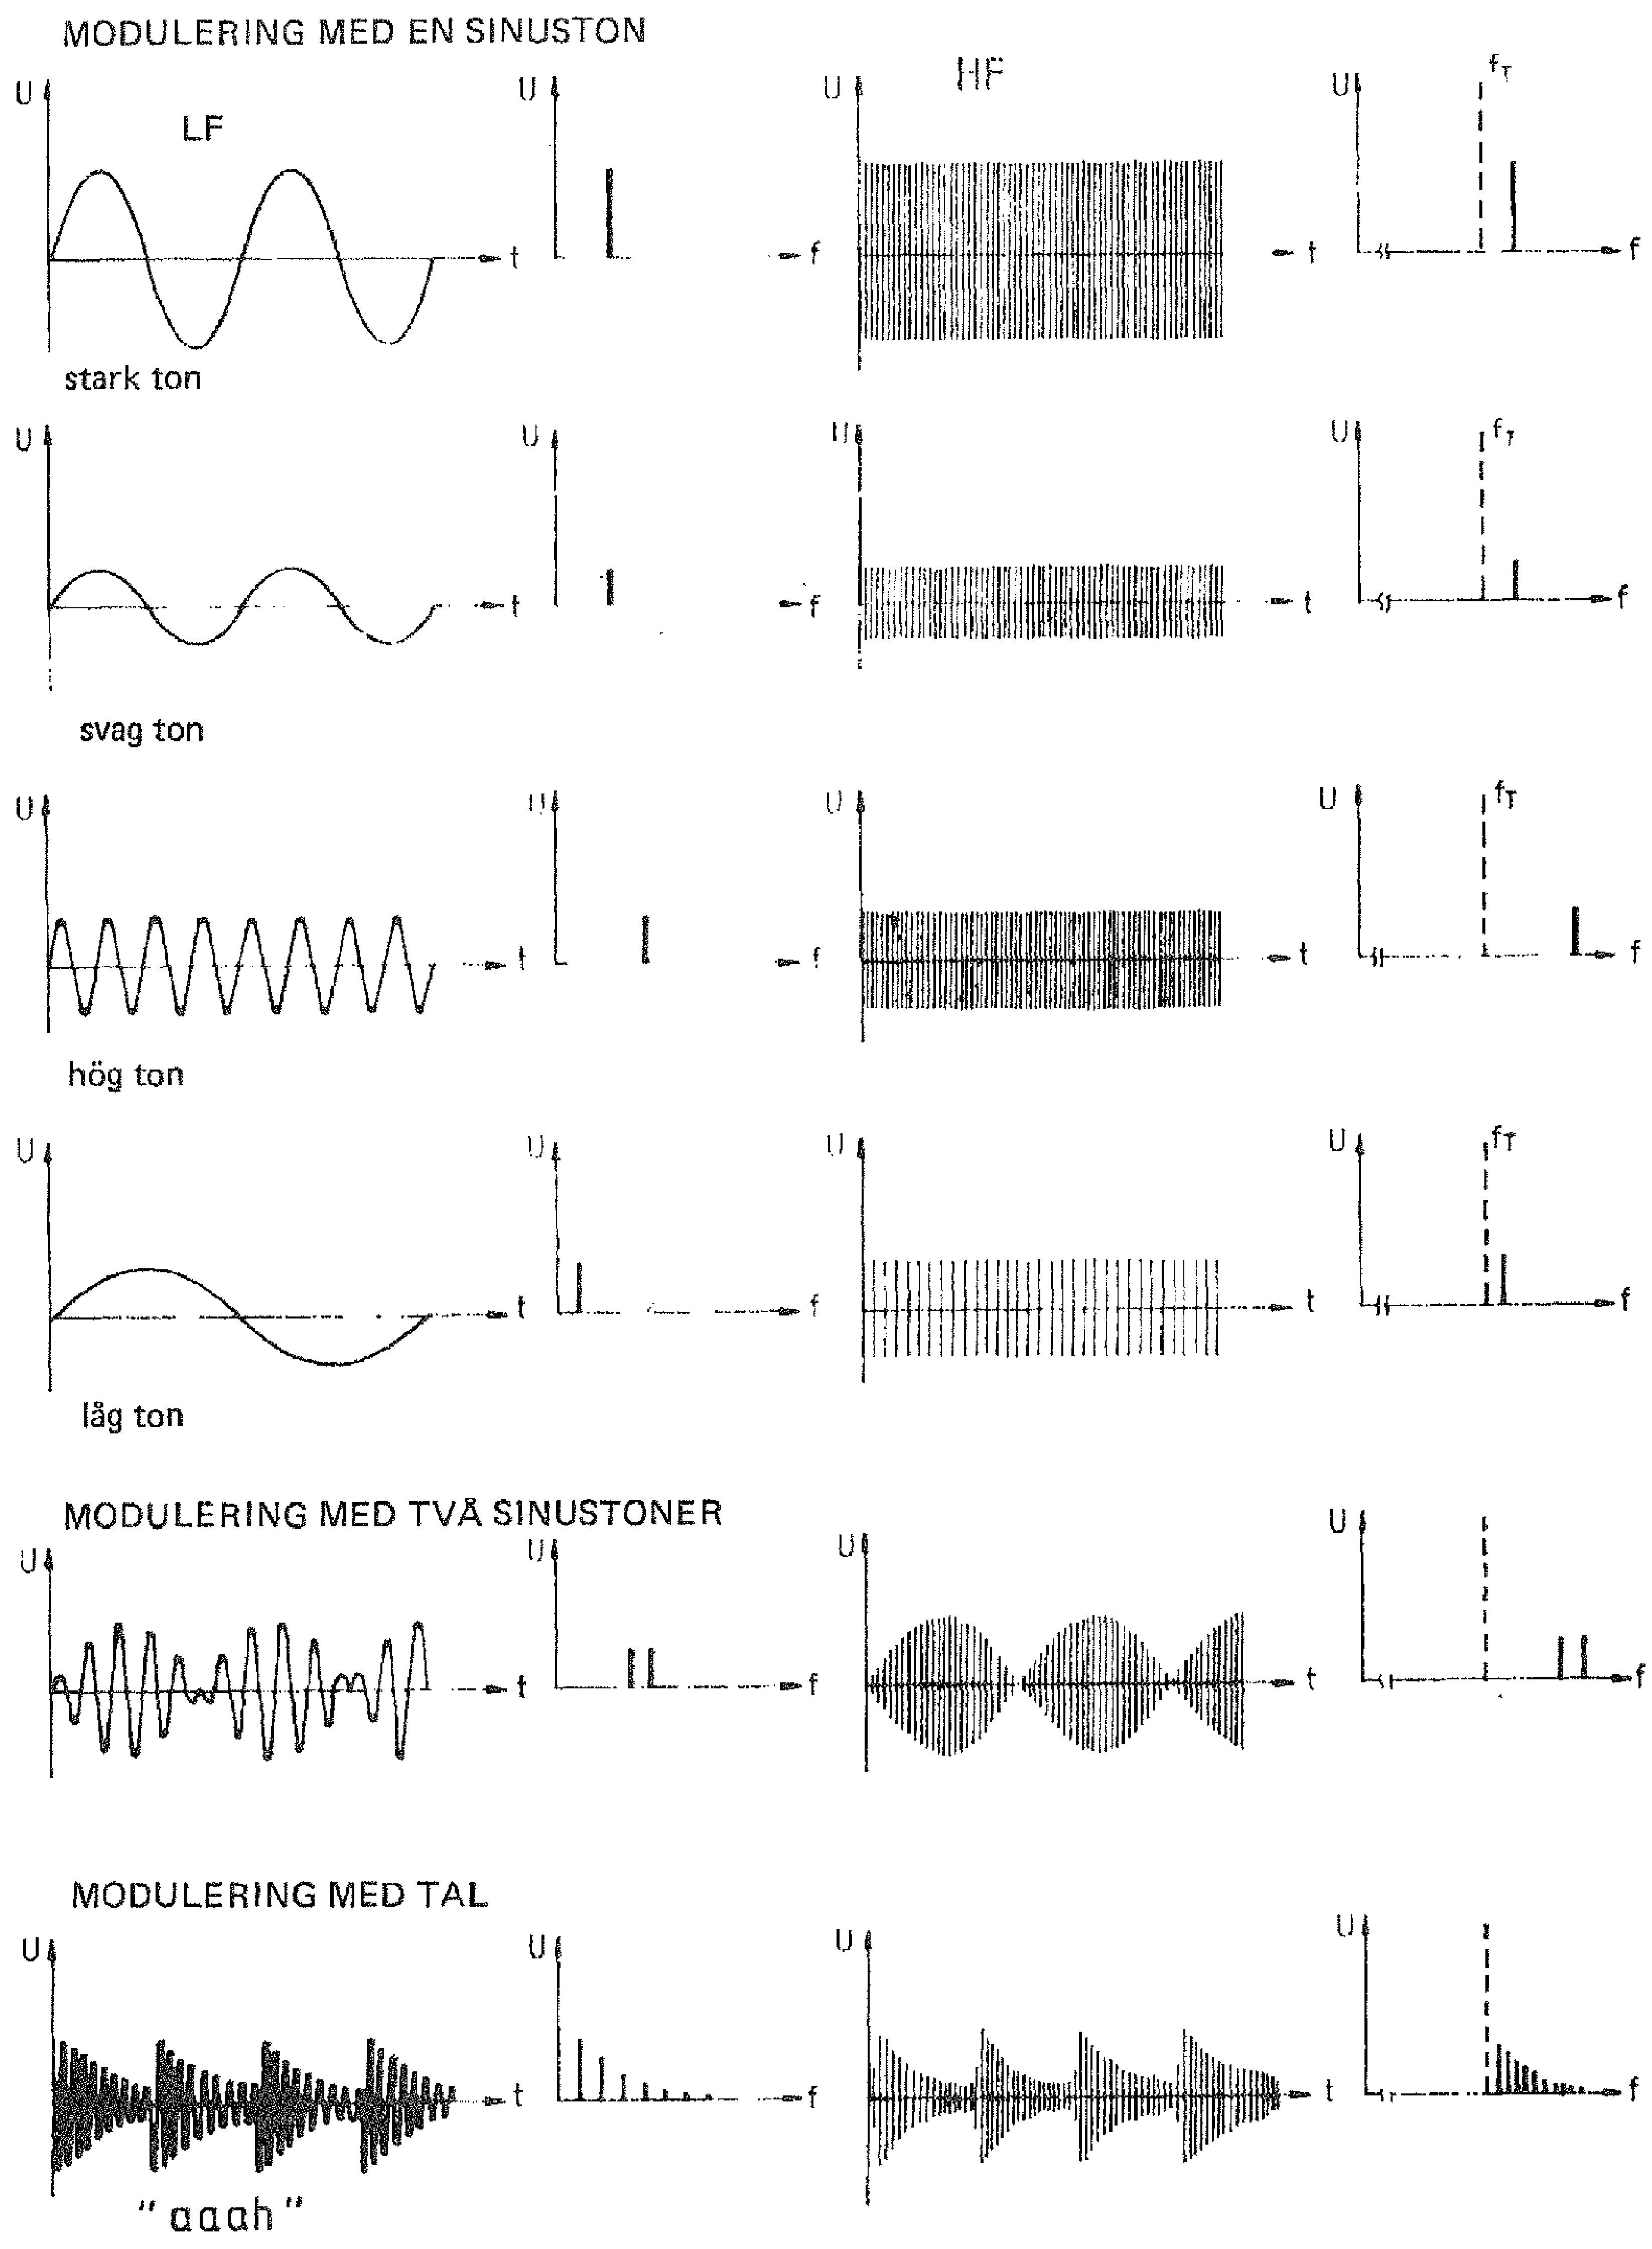
\includegraphics[width=\textwidth]{images/cropped_pdfs/bild_2_1-29.pdf}
\caption{Sidbandslägen vid SSB}
\label{fig:BildII1-29}
\end{figure}

Bild \ref{fig:BildII1-29}.

LF-signalens amplitud bestämmer amplituden på sidofrekvensen.

LF-signalens frekvens bestämmer sidofrekvensens avstånd från bärvågsfrekvensen
(bärvågen undertryckt).

Bandbredden på den utsända signalen är skillnaden mellan högsta och lägsta
modulerande frekvens i signalen:

t.ex. \(b = 3~kHz - 0,3~kHz = 2,7~kHz\)

\subsubsection{Fördelar med J3E-modulation}
Bra verkningsgrad vid J3E-modulation jämfört med vid A3E-modulation
(traditionell AM). Effekten i det utsända sidbandet motsvarar den i ett av
sidbanden vid A3E. Hela den utsända effekten finns alltså i ett enda sidband,
som överför hela informationen.

I sändningspauserna sänds ingen effekt ut. Bandbredden är mindre än hälften av
den vid A3E. Vid mottagning av en J3E-sändning (SSB) är det mindre besvär med
interferenstoner från J3E-sändningar på närliggande frekvenser, eftersom ingen
bärvåg och endast ett sidband sänds ut.

\subsubsection{Nackdelar med J3E-modulation}
J3E-modulation medför mera komplicerade apparater, både för mottagning och
sändning. En J3E-signal blir förvrängd och hörs i fel tonläge, om mottagaren
inte är inställd på exakt rätt frekvens.

\subsection{Vinkelmodulation}
\textbf{HAREC a.\ref{HAREC.a.1.8.3a}\label{myHAREC.a.1.8.3a}}
\index{vinkelmodulation}

Termen vinkelmodulation är samlingsnamnet för frekvensmodulation (FM) och
fasmodulation (PM). Ofta sägs utrustningar vara för frekvensmodulation, när de
antingen är för frekvens- eller fasmodulation. Det finns alltså skillnader och
likheter mellan dessa system, vilka emellertid inte är oberoende av varandra,
eftersom frekvensen i en signal inte kan varieras utan att fasen också
varieras, och vice versa.

Hur effektiv kommunikationen då är, beror mest på mottagningsmetoderna. I båda
fallen uppfattas ändringar i den mottagna signalens frekvens och fasläge.
Amplitudändringar uppfattas däremot inte. De flesta störningar -- särskilt
pulserande sådana som från tändningssystem -- kommer att därför att skiljas bort.

För att effektivt utnyttja fördelarna med vinkelmodulation, antingen det är
frekvens eller fasmodulation, behövs tillräckligt frekvensutrymme. Det innebär
att främst högre frekvensband kommer i fråga.

\subsection{Frekvensmodulation (även kallat FM)}
\textbf{HAREC
  a.\ref{HAREC.a.1.8.3b}\label{myHAREC.a.1.8.3b},
  a.\ref{HAREC.a.1.8.6d}\label{myHAREC.a.1.8.6d}
}
\index{frekvensmodulation}
\index{FM}

\begin{figure}
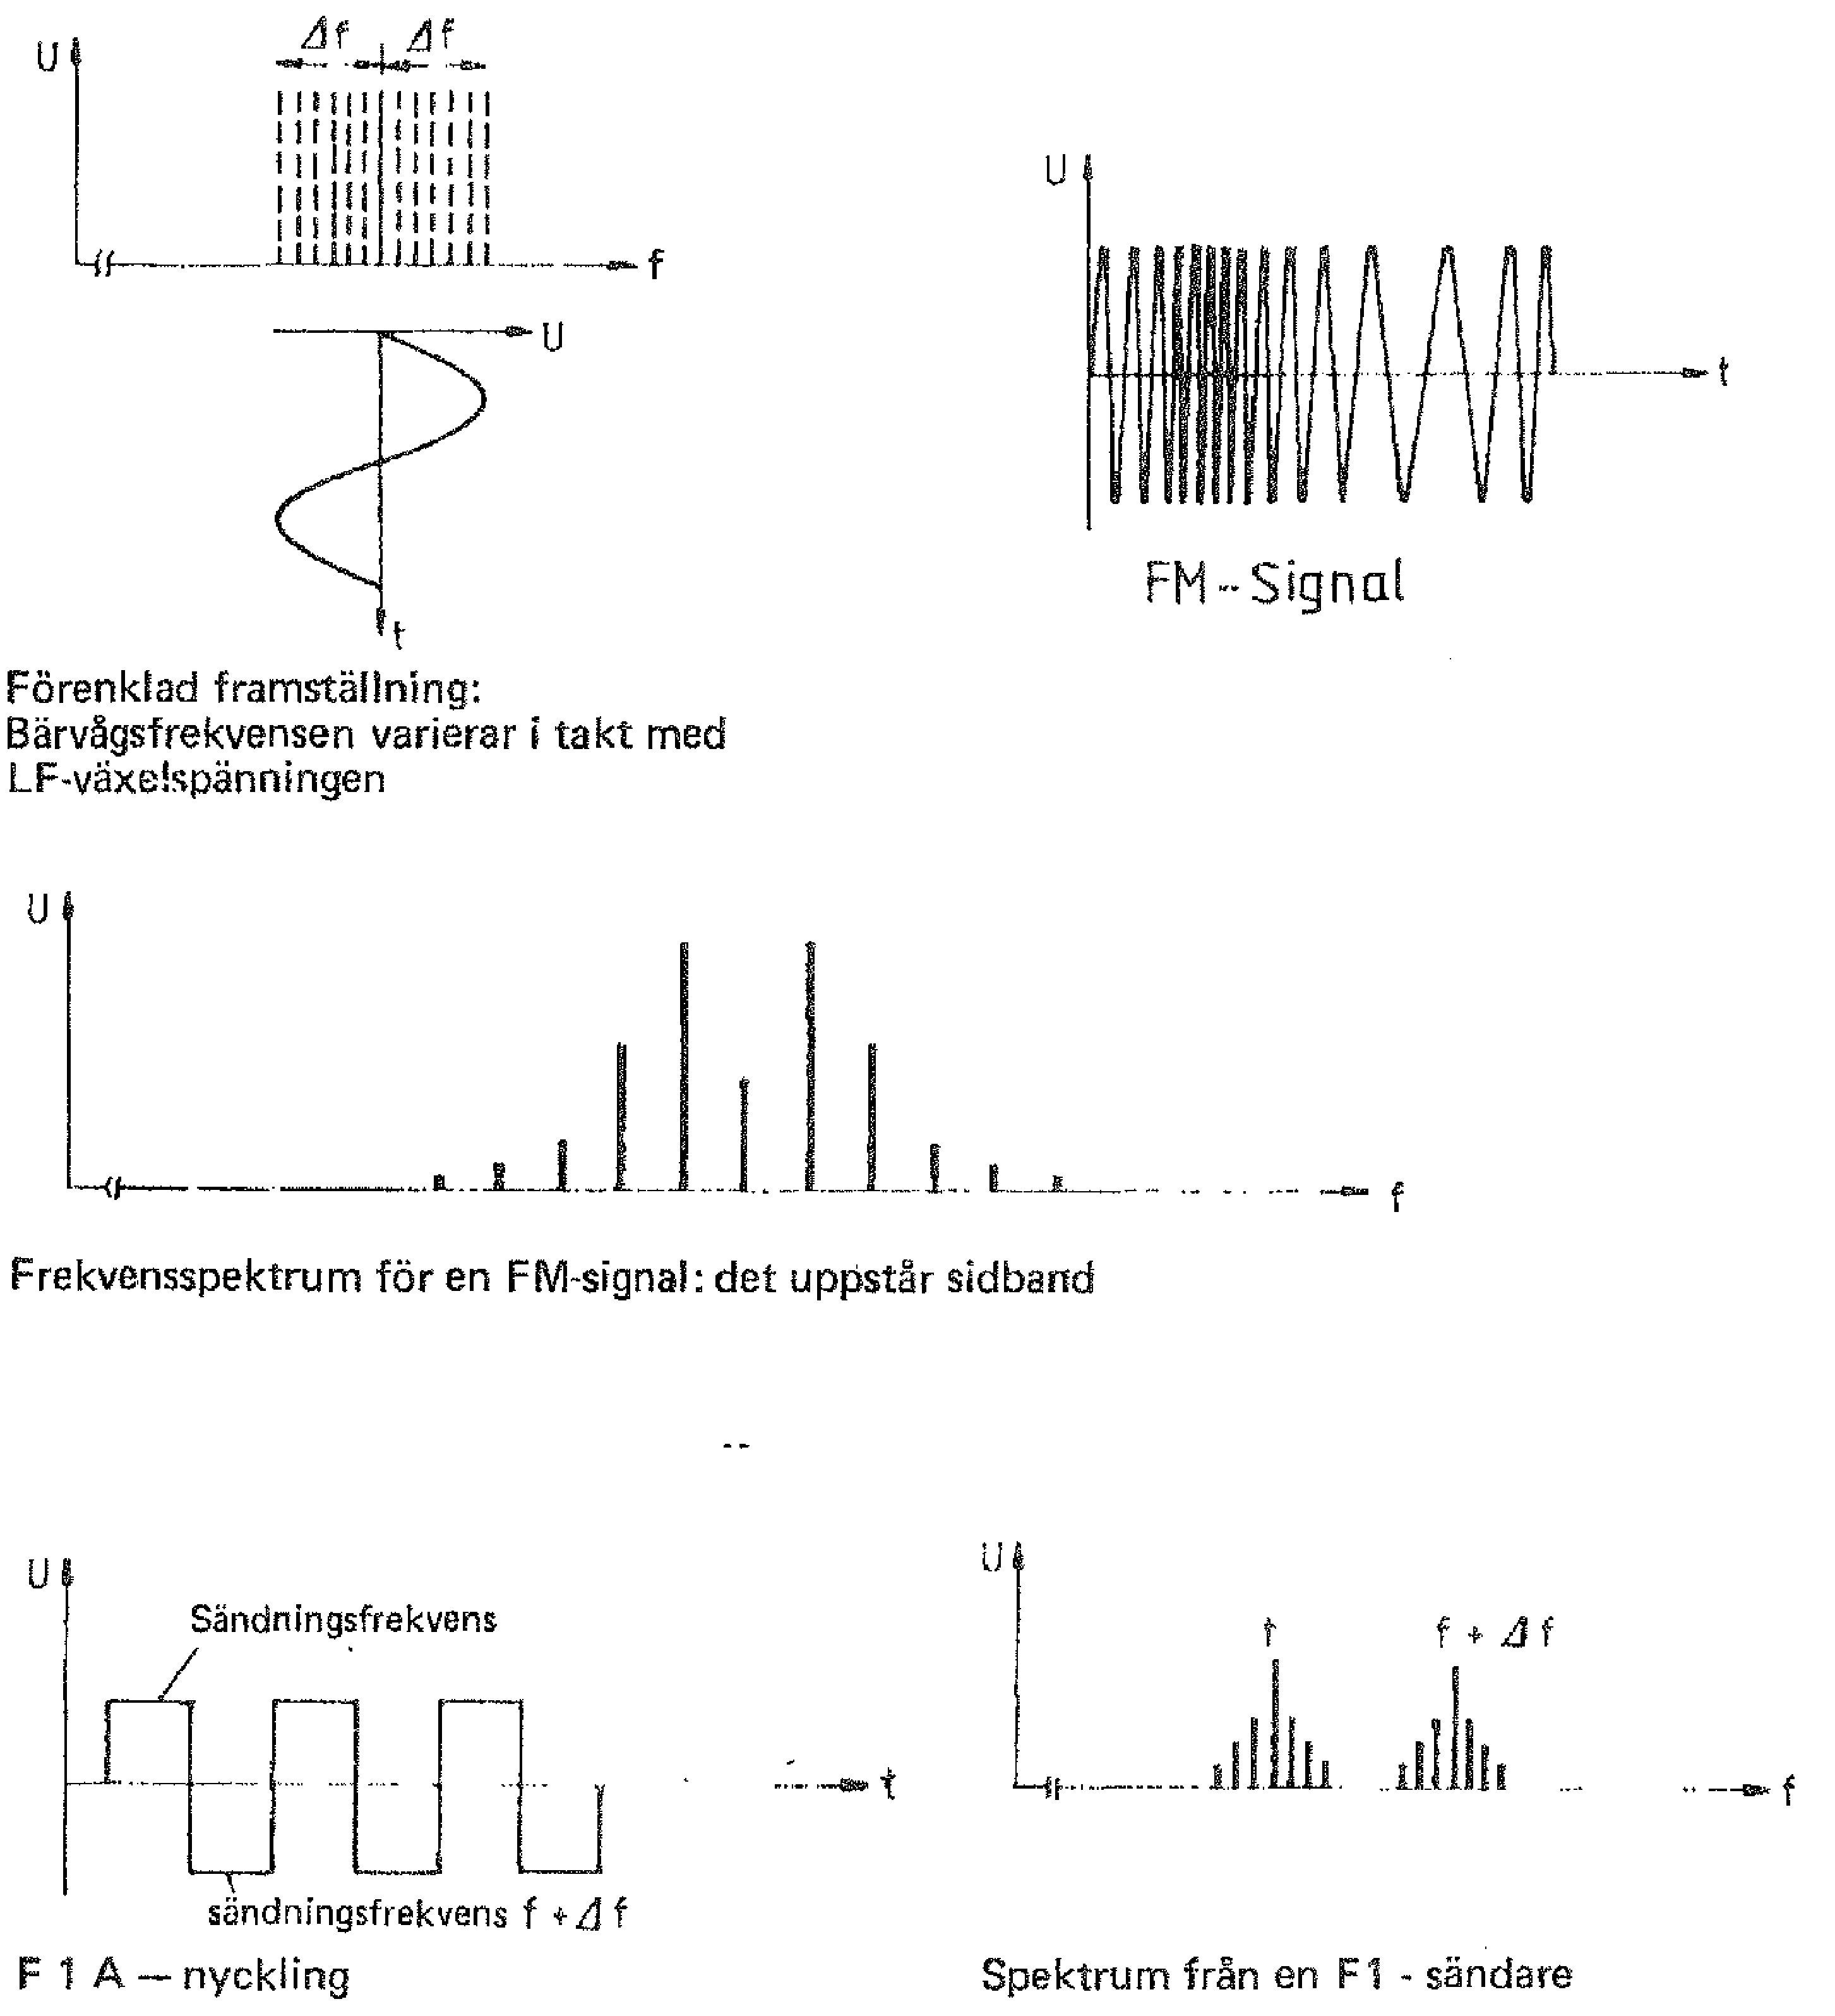
\includegraphics[width=\textwidth]{images/cropped_pdfs/bild_2_1-30.pdf}
\caption{Frekvensmodulation}
\label{fig:BildII1-30}
\end{figure}

Bild \ref{fig:BildII1-30} (överst och i mitten).

Vid frekvensmodulation varierar bärvågens frekvens i takt med den modulerande
signalens amplitud och polaritet. På bilden ökar bärvågens frekvens när den
modulerande signalen är positiv (första halvperioden) och minskar när den
modulerande signalen är negativ (andra halvperioden). Bilden visar att
perioderna i den modulerade bärvågen tar kortare tid (har högre frekvens), när
den modulerande signalen är positiv, och mertid (har lägre frekvens) när den
modulerande signalen är negativ. Bärvågen kommer alltså att pendla omkring ett
medelvärde, d.v.s. vara frekvensmodulerad.

Frekvensavvikelsen \(\Delta f\) (deviationen) från bärvågens vilofrekvens är
vid varje tillfälle proportionell till den modulerande signalens amplitud.
Sålunda är deviationen liten när den modulerande signalens amplitud är liten
och störst när amplituden når sitt toppvärde, antingen amplituden är positiv
eller negativ. Vid en modulationsfrekvens av 300~Hz varierar bärvågsfrekvensen
300 gånger per sekund, vid 3~kHz -- 3000 gånger per sekund.

Likspänningsnivåer kan överföras med FM, eftersom en motsvarande
frekvensavvikelse kan framställas.

Bilden visar också vad som oftast sägs, att bärvågsamplituden inte ändras av
modulationen. Detta är emellertid bara delvis sant, eftersom såväl
bärvågsamplitud som sidbandsamplitud varierar med modulationsindex, vilket
förklaras nedan.

\subsubsection{Sidbanden vid vinkelmodulation}

Vid AM produceras endast ett sidbandspar med samma innehåll, ett över och ett
under bärvågsfrekvensen. Vid vinkelmodulation, både vid FM och PM, produceras
däremot flera sidbandspar över och under bärvågsfrekvensen. Dessa sidband
uppträder på multiplerna av varje modulerande frekvens. Vid basband med samma
frekvensomfång har därför en vinkelmodulerad signal större bandbredd än en
AM-signal.

Vid vinkelmodulation beror antalet sidband på sambandet mellan den modulerande
frekvensen, frekvensdeviationen och modulationsindex.

\subsubsection{Bandbredden vid vinkelmodulation}

Bild \ref{fig:BildII1-30} (nederst).

Vi gör tankeexperimentet att en FM-sändare moduleras med en fyrkantsvåg.
Frekvensen kommer då att hoppa växelvis mellan frekvenserna \(f\) och
\(f + \Delta f\). Sättet kallas FSK (frekvensskiftnyckling) och används t.ex.
vid sändning av radiofjärrskrift (RTTY, AMTOR, Paketradio etc.).

Vi föreställer oss två sändare, som sänder varannan gång, varav den ena sänder
frekvensen \(f\) och den andra sänder \(f + \Delta f\). Båda sändarnas
HF-signaler kommer då att bilda ett frekvensspektrum, som förutom \(f\) och
\(f + \Delta f\) även innehåller sidofrekvenser.

Bredden på detta spektrum beror bl.a. på nycklingsfrekvensen. Eftersom en
fyrkantsvåg innehåller summan av dess grundfrekvens och övertoner, kommer alla
dessa toner att modulera vardera sändaren. De högsta modulerande
LF-frekvenserna alstrar sidofrekvenserna längst ut från vilofrekvensen.
LF-signalens frekvensspektrum påverkar alltså HF-signalens bandbredd.

Spektrum nederst i bilden är en förenklad framställning av
frekvensskiftnyckling.

Vid modulation med en sinussignal istället för med en fyrkantssignal, uppstår ett
frekvensspektrum som på överst i bilden.

\paragraph{Frekvensdeviation och modulationsindex}
\textbf{HAREC a.\ref{HAREC.a.1.8.4}\label{myHAREC.a.1.8.4}}
\index{frekvensdeviation}
\index{modulationsindex (m)}
\index{symbol!\(m\) modulationsindex}

\begin{figure}
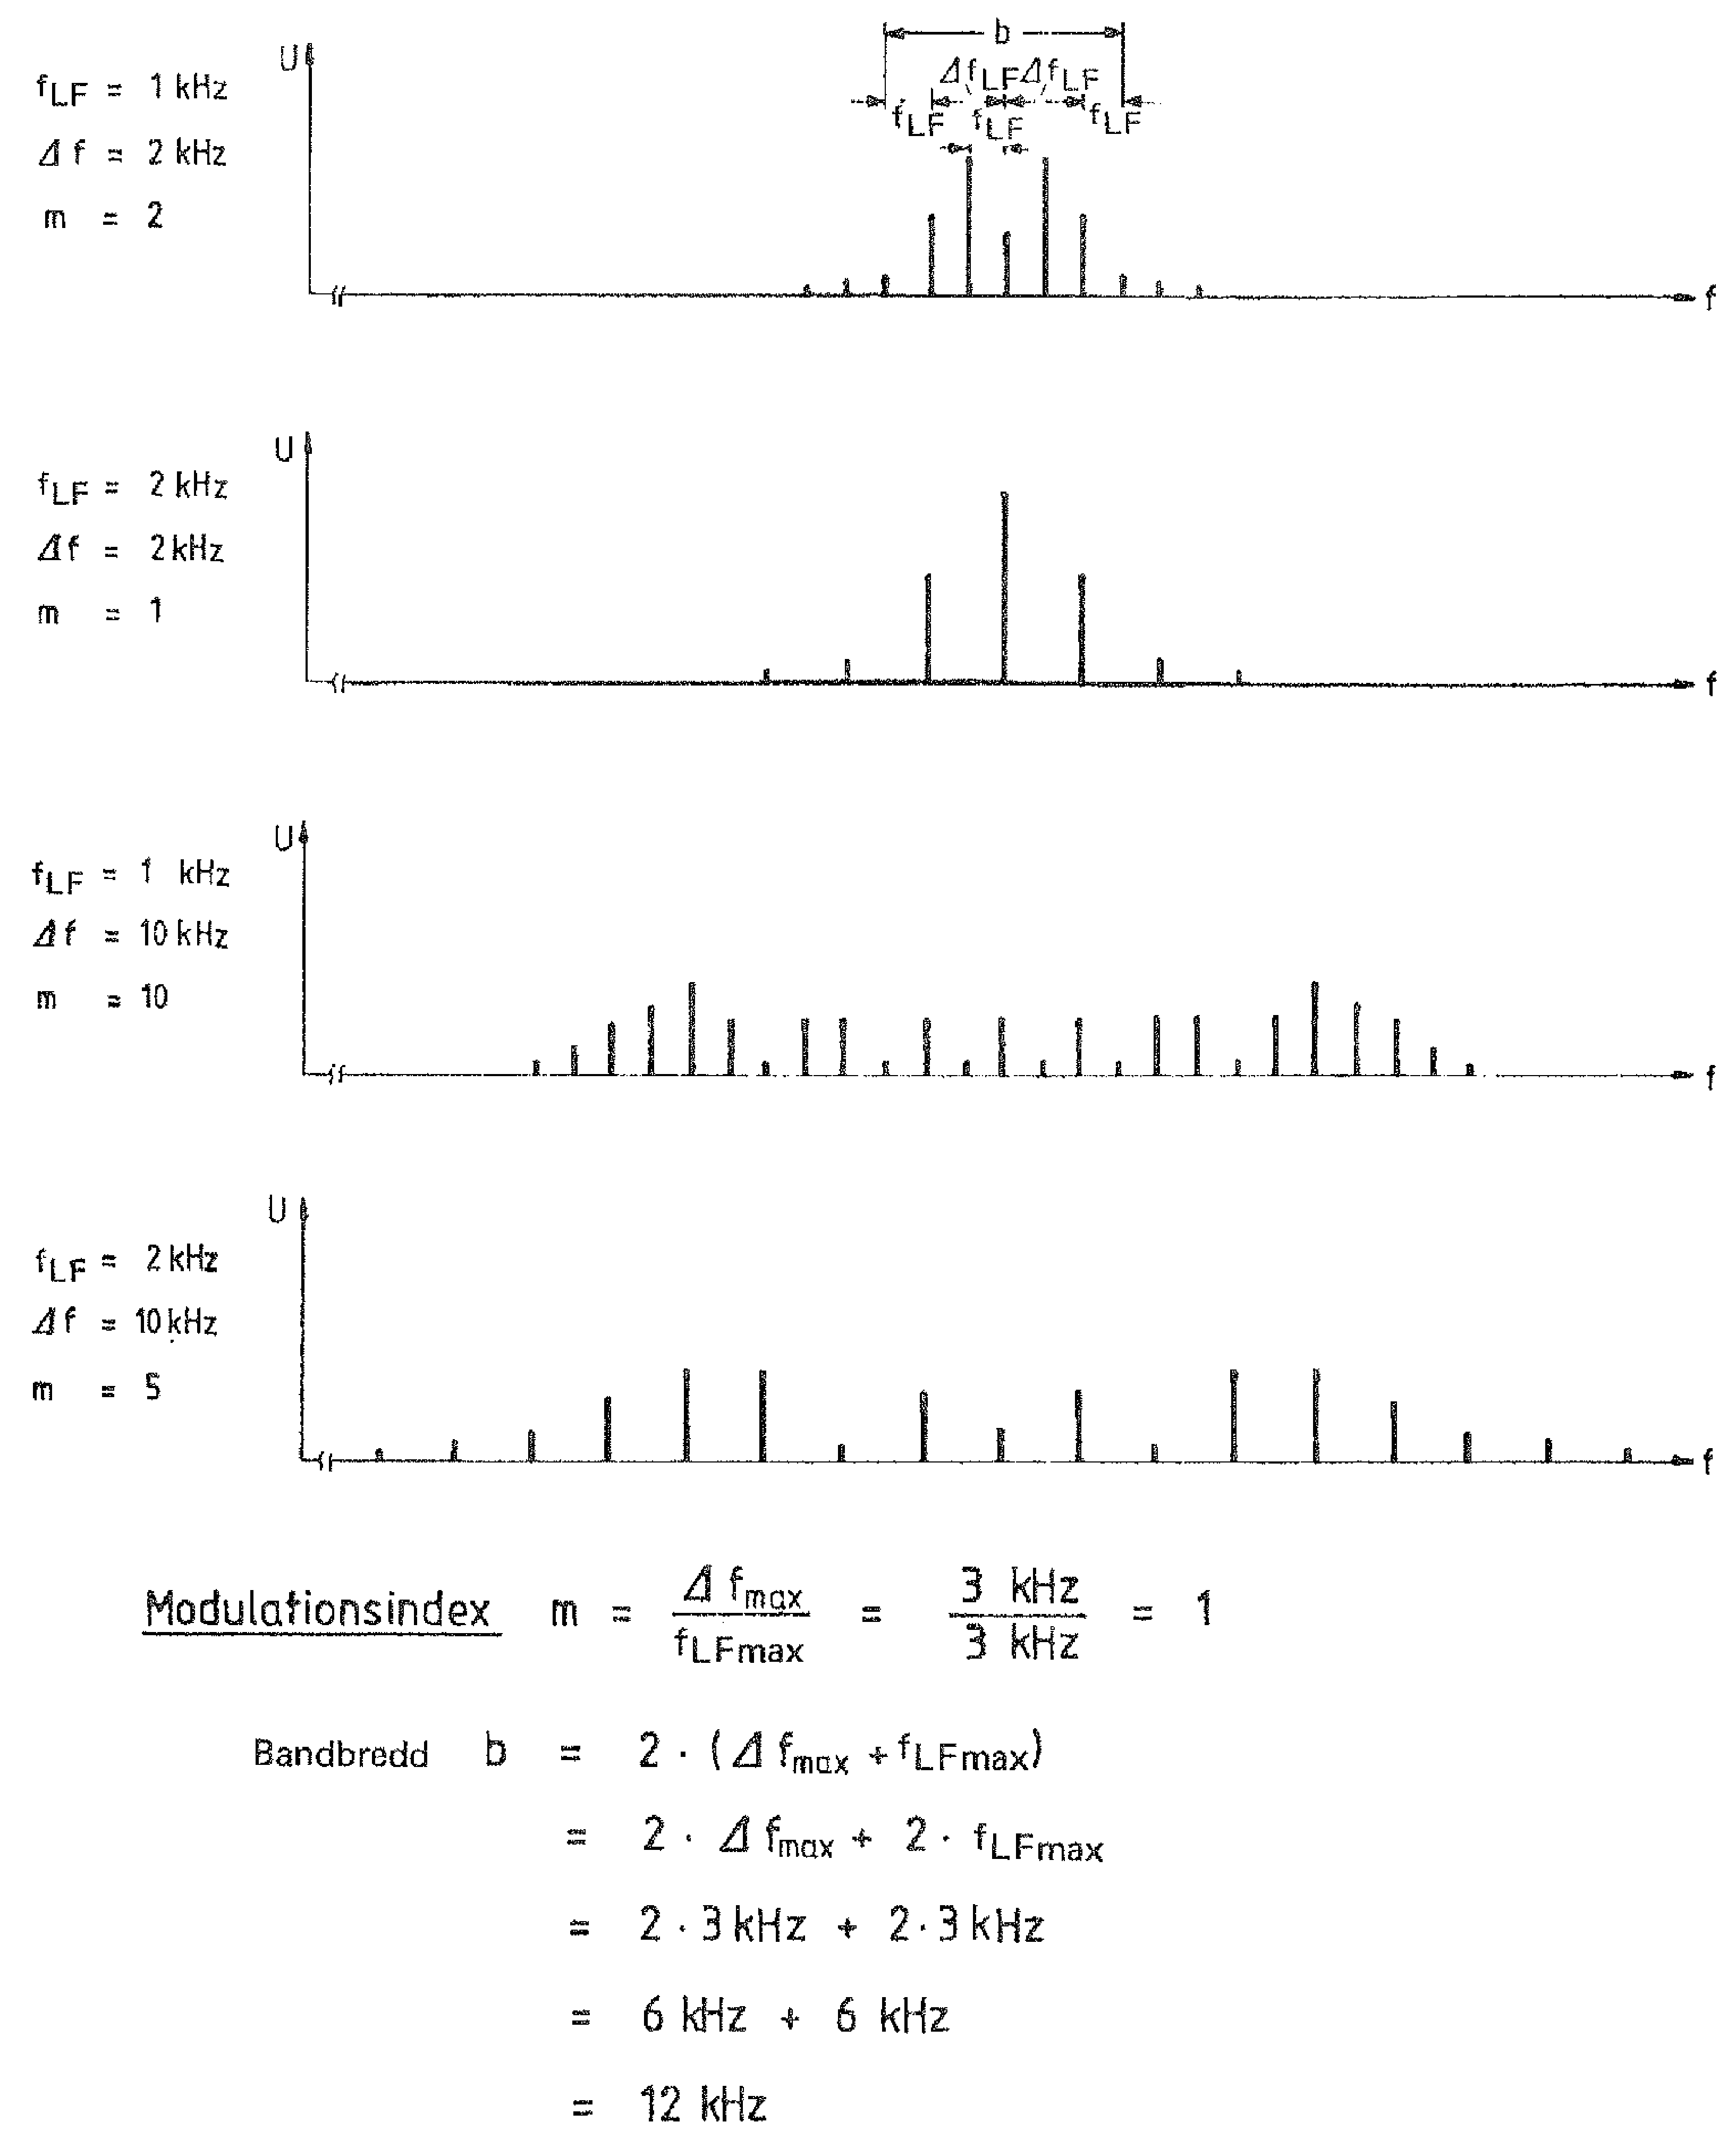
\includegraphics[width=\textwidth]{images/cropped_pdfs/bild_2_1-31.pdf}
\caption{Sidbandsspektrum vid FM-modulering med 1 sinuston}
\label{fig:BildII1-31}
\end{figure}

Bild \ref{fig:BildII1-31}.

Vid vinkelmodulation uppstår talrika sidofrekvenser, som beror av den
modulerande frekvensen \(f_{LF}\). Amplitudfördelningen mellan sidofrekvenserna
står i förhållande till deviationen, varvid deras amplitud blir mindre desto
längre bort från bärvågen de är.

I praktiken anses en sidofrekvens försumbar när dess amplitud är mindre än 1~\%
av amplituden för omodulerad bärvåg.

För beräkning av bandbredden används begreppet modulationsindex m, vilket är
kvoten av maximal deviation \(\Delta f\) och högsta frekvensen \(f_{LF}\).

\(m = \dfrac{\Delta f_{max}}{f_{LFmax}}\)

Inom amatörradion är det vanligt att arbeta med \(\Delta f_{max} = 3 kHz\) och
\(f_{LFmax} = 3 kHz\), d.v.s. \(m = 1\).

Vid modulationsindex \(m = 1\), gäller följande
formel för bandbredden \(b\)

\(b = 2 \cdot ( \Delta f_{max} + f_{LFmax}) = 2 \cdot \Delta f_{max}
 + 2 \cdot f_{LFmax}\)

Med ovan nämnda värden blir bandbredden \(b = 2 \cdot (3 kHz + 3 kHz)
 = 12 kHz\)

Bandbredden ökar således både med ökande deviation och ökande modulerande
frekvens. För att inte interferera med trafik på grannkanalerna måste såväl
deviation som frekvensen på den modulerande signalen begränsas. En
deviationsbegränsare begränsar amplituden på denna signal. Ett lågpassfilter
reducerar den distorsion, som uppstår av begränsningen. Vidare undertrycks
modulerande frekvenser högre än 3~kHz, vilket är tillräckligt för överföring
av tal.

\paragraph{Jämförelse}

En VHF-rundradiosändare är tilldelad ett större frekvensutrymme och kan därför
använda mycket större bandbredd.

Där är \(\Delta f_{max} = 75 kHz\) och \(f_{LFmax} =15 kHz\), därmed är
\(m = \frac{75}{15} = 5\) och \(b = 2 \cdot (75 + 15) = 180 kHz\).

Som framgår av tabellen på nästa uppslag varierar bärvågens liksom
sidofrekvensernas inbördes amplitud med modulationsindex. Detta ska jämföras
med AM där bärvågens amplitud är konstant och endast sidbandens amplitud
varierar.

Vid vinkelmodulation utsläcks bärvågen \(A_0\) vid modulationsindex 2.404. Den
blir sedan ''negativ'' vid högre index, vilket betyder att den återkommer, men
att dess fasläge blir omvänt. I vinkelmodulation tas energin i sidbanden från
bärvågen, vilket innebär att den totala effekten förblir densamma oavsett
modulationsindex.

\paragraph{Kännetecken för sändningsslaget F3E (FM)}
\index{F3E}

Fördelar: F3E-sändaren är enkel till sin uppbyggnad och hög överföringskvalitet
uppnås vid stor bandbredd, störningar från amplitudmodulerade signaler t.ex.
tändgnistor undertrycks i mottagaren.

Nackdelar: En relativt stor bandbredd behövs för överföring av ett basband med
stort frekvensomfång. Sändaren måste avge full effekt, även när modulation inte
sker.

\begin{table*}[h]
\begin{center}
\begin{tabular}{ll|l|l|l|l|l|l|l|l|}
\cline{3-9}
&\multicolumn{1}{l}{}  & \multicolumn{7}{|c|}{Modulationsindex} \\ \cline{3-9}
&\multicolumn{1}{l|}{}  &   1   &   2   &    3   &    4   &    5   &    6   &    7   \\ \hline
\multicolumn{1}{|c|}{\multirow{11}{*}{\rotatebox[origin=c]{90}{Relativ amplitud på}}}&\(A_0\) & 0,765 & 0,224 & -0,260 & -0,397 & -0,178 &  0,151 &  0,300 \\
\multicolumn{1}{|c|}{}&\(A_1\) & 0,440 & 0,577 &  0,334 & -0,066 & -0,328 & -0,277 & -0,005 \\
\multicolumn{1}{|c|}{}&\(A_2\) & 0,115 & 0,353 &  0,486 &  0,364 &  0,047 & -0,243 & -0,301 \\
\multicolumn{1}{|c|}{}&\(A_3\) & 0,020 & 0,129 &  0,309 &  0,430 &  0,365 &  0,115 & -0,168 \\
\multicolumn{1}{|c|}{}&\(A_4\) &       & 0,034 &  0,132 &  0,281 &  0,391 &  0,358 &  0,158 \\
\multicolumn{1}{|c|}{}&\(A_5\) &       & 0,016 &  0,043 &  0,132 &  0,261 &  0,362 &  0,348 \\
\multicolumn{1}{|c|}{}&\(A_6\) & \multicolumn{2}{c|}{} &  0,011 &  0,049 &  0,131 &  0,246 &  0,339 \\
\multicolumn{1}{|c|}{}&\(A_7\) & \multicolumn{3}{c|}{} &  0,015 &  0,053 &  0,130 &  0,234 \\
\multicolumn{1}{|c|}{}&\(A_8\) & \multicolumn{4}{c|}{}           &  0,018 &  0,057 &  0,128 \\
\multicolumn{1}{|c|}{}&\(A_9\) & \multicolumn{4}{c}{} &        &  0,021 &  0,059 \\
\multicolumn{1}{|c|}{}&\(A_{10}\) & \multicolumn{5}{c}{Tomma fält för \(A_n\) under 0,01 (1 \%)} &  &  0,024 \\ \hline
\end{tabular}
\end{center}
\caption{Relativa amplituden på bärvåg $A_0$ och sidofrekvenser $A_1$--$A_{10}$ vid
modulationsindex 1--7 (Vid omodulerad bärvåg är modulationsindex 0. Då är
bärvågens relativa amplitud 1,0)}
\end{table*}


\subsection{Fasmodulation (även kallat PM)}
\index{fasmodulation}
\index{PM}

Vid fasmodulation varierar bärvågens fasläge i förhållande till ett
referensvärde. Vid PM är frekvensändringen -- deviationen -- direkt proportionell
till hur snabbt fasläget på den modulerande frekvensen ändras och till den
totala fasändringen. Hastigheten på fasändringen är direkt proportionell till
frekvensen på den modulerande frekvensen och till den momentana amplituden på
den modulerande signalen.

Det betyder att deviationen i PM-system ökar både med den momentana amplituden
och frekvensen på den modulerande signalen. Detta att jämföras med FM-system där
deviationen är proportionell till den momentana amplituden på den modulerande
signalen.

I PM-system uppfattar demodulatorn i mottagaren endast momentana ändringar i
bärvågsfrekvensen. Till skillnad från vid FM, så kan därför ändringar i
likspänningsnivåer överföras endast om en fasreferens används.

Med konstant amplitud på insignalen till modulatorn, så är vid PM
modulationsindex konstant oavsett modulerande frekvens, medan vid FM
modulationsindex varierar med den modulerande frekvensen.

\subsection{Frekvens- och fasmodulation jämförs}

\begin{itemize}
\item Frekvensmodulation (FM) alstras genom att sändarens oscillatorfrekvens
varieras (devieras) i takt med den modulerande signalen (t.ex. tal). Det gör man
genom att variera resonansfrekvensen i den svängningskrets som styr
oscillatorfrekvensen.

\item Fasmodulation (PM) alstras vanligen genom att efter sändaroscillatorn
variera den modulerande signalens fasläge i förhållande till en omodulerad
bärvåg -- s.k. fasmodulering. Det gör man genom att variera resonansfrekvensen i
en svängningskrets efter oscillatorn- d.v.s. utan att påverka
oscillatorfrekvensen.

\item I båda fallen ändrar man alltså resonansfrekvensen i en svängningskrets i
takt med frekvensen i den modulerande spänningen, men att denna krets har olika
placering i FM-sändare respektive PM-sändare.

\item I sändaren alstras det i båda fallen utfrekvenser som devierar från
oscillatorns vilofrekvens. Graden av deviation skiljer emellertid vid FM och PM.
Vid FM är deviationen proportionell mot amplituden på den modulerande
underbärvågen medan deviationen vid PM är proportionell mot produkten av den
modulerande underbärvågens amplitud och frekvens.

\item Den hörbara skillnaden mellan FM och PM är därför en annorlunda
frekvensgång. Vid samtidig användning av PM-sändare och FM-mottagare är det
alltså lämpligt att justera frekvensgången i PM-sändarens modulator, lämpligen
med 6~dB dämpning per oktav ökad frekvens.
\end{itemize}

\subsection{Pulsmodulation}
\index{pulsmodulation}
\index{PWM}
\index{PAM}
\index{PPM}

Pulsmodulation används mest i mikrovågsområdet. Pulsmodulerade signaler sänds
vanligen som en serie korta pulser åtskilda av relativt långa pauser utan
modulering.

En typisk sändning kan bestå av pulser med en längd av 1 \(\mu\)s och en
frekvens av 1000~Hz. Toppeffekten på en pulssändning är därför mycket högre än
dess medeleffekt

Före WARC 79 var symbolen för all pulssändning P. Därefter används P endast för
omodulerade pulståg. Annan pulsmodulation har följande symboler

\begin{description}
\item[K] -- puls-/amplitudmodulation (PAM)
\item[L] -- pulsviddmodulation (PWM)
\item[M] -- pulsposition/fasmodulation (PPM)
\item[Q] -- vinkelmodulation under pulsen
\item[V] -- kombination av dessa eller annat sätt.
\end{description}

\begin{table*}[h]
\begin{center}
\begin{tabular}{|l|l|l|l|l|}
\hline
Sändningsslag & Amplituden på & Tonhöjden på & Bandbredden b      & För stor amplitud \\
              & LF-signalen   & LF-signalen  & förhåller sig till & på LF-signalen \\
              & påverkar      & påverkar     &                    & medför \\ \hline
A3E (AM) & amplituden i   & sidofrekvenser- & LF-signalens    & övermodulering \\
         & båda sidbanden & nas avstånd    & högsta frekvens & och för stor bandbredd \\
         &                & från bärvågen  & & \\
J3E (SSB)& amplituden på  & sidofrekvenser- & skillnaden mellan & för stor bandbredd,\\
         & utsänt sidband & nas avstånd    & LF-signalens      & överstyrning av\\
         &                & från bärvågen  & högsta och lägsta & förstärkarsteg\\
         &                &                & frekvens          & \\
F3E (FM) & deviationen    & hastigheten på & dubbla summan     & för stor deviation,\\
         &                & bärvågens      & av största devia- & för stor bandbredd\\
         &                & frekvens-      & tion och högsta   & \\
         &                & ändring        & LF-frekvens       & \\ \hline
\end{tabular}
\end{center}
\caption{Jämförelse mellan några vanliga sändningsslag inom amatörradio}
\end{table*}

\subsection{Digital modulationer}
\textbf{HAREC a.\ref{HAREC.a.1.8.8}\label{myHAREC.a.1.8.8}}
\index{digital modulation}

Utöver de klassiska analoga modulationsmetoder finns ett antal digitala
modulationsformer. De är anpassade för transmission av binär data. I viss mån
kan CW ses som digital modulation där en 0 moduleras utan bärvåg och 1 moduleras
med bärvåg. Det finns dock flera andra modulationsmetoder som FSK, 2-PSK/BPSK,
4-PSK och QAM som presenteras i följande delavsnitt.

\subsubsection{Frekvensskift modulation -- FSK}
\textbf{HAREC a.\ref{HAREC.a.1.8.8a}\label{myHAREC.a.1.8.8a}}
\index{frekvensskift modulation}
\index{Frequency Shift Keying (FSK)}
\index{FSK}
\index{frekvensmodulation}
\index{FM}
\index{GFSK}
\index{Gaussiskt filter}
\index{C4FM}
\index{JT65}
\index{JT9}

\emph{Frekvensskift modulation} (eng. \emph{Frequency Shift Keying (FSK)})
skiljer sig från CW modulationen med att den ändrar frekvensen, dvs. är en
variant av frekvensmodulation. I den enklaste formen, binär FSK, så växlar man
mellan 2 frekvenser, där en frekvens får representera 0 och den andra får
representera 1. Denna metod har används för modem på telefon-förbindelser,
så som Bell 103.

Eftersom varje växling mellan frekvenser ger avbrott i bägge signalerna,
likt nycklingen i CW, så kommer de skapa sidband. Av det skälet filtrerar man
gärna signalen, och använder man ett Gaussiskt filter får man Gaussian Frequency
Shift Keying (GFSK) som används av t.ex. GSM telefoni.

Man kan använda fler än 2 frekvenser, t.ex. används 4 frekvenser i Continuous
4 level FM (C4FM) i Phase 1 radios i Project 25 samt Fusion.

Frekvensskift används även för att sända långsamma meddelanden där JT65
använder 65 frekvenser den skiftar mellan, medans JT9 använder 9 frekvenser.

\subsubsection{Binär fasskift modulation -- 2-PSK \& BPSK}
\textbf{HAREC a.\ref{HAREC.a.1.8.8b}\label{myHAREC.a.1.8.8b}}
\index{binär fasskift modulation}
\index{fasskift modulation!binär}
\index{2-PSK}
\index{fasskift modulation!2-PSK}
\index{BPSK}
\index{fasskift modulation!BPSK}
\index{Costas loop}

Istället för att modulera frekvensen kan man modulera polariteten eller fasen.
En sådan modulationsform är \emph{binär fasskift modulation} (eng.
\emph{Binary Phase Shift Keying (BPSK)} eller \emph{2-state Phase Shift Keying
(2-PSK)}. Förenklat kan man säga att bärvågen moduleras med +1 eller -1,
ofta med +1 representerande 0 och -1 representerande 1.

En nackdel med BPSK är att blir polariteten förväxlad så kommer meddelandet
att bli inverterat, dvs. 0 blir 1 och 1 blir 0. BPSK behöver därför också
kompletteras med annan digital modulation för att hantera polariteten, något
som i allmänhet kan åstadkommas enkelt.

BPSK används t.ex. av satellitnavigationssystem som GPS, GLONASS och Galileo.
För att återvinna BPSK behöver man ofta en speciell variant av PLL-loop känd
som \emph{Costas loop}, eftersom en normal PLL-loop klarar inte av
teckenändringarna på signalen.

\subsubsection{Fyrnivå fasskiftmodulation -- 4-PSK}
\textbf{HAREC a.\ref{HAREC.a.1.8.8c}\label{myHAREC.a.1.8.8c}}
\index{4-PSK}
\index{fasskift modulation!4-PSK}
\index{kvadratur-modulering}
\index{quadrature modulation}
\index{in phase}
\index{quadrature}
\index{I/Q modulation}

Fasskiftmodulation kan även göras med flera nivåer, och 4 olika fas-lägen
kan användas och kallas då för \emph{fyrnivå fasskiftmodulation} (eng.
\emph{4-state Phase Shift Keying (4-PSK)}.

Istället för 180 graders fas-skift (0 och 180 grader) som 2-PSK/BPSK använder
så använder man 360/4 dvs. 90 graders fas-skift mellan symbolerna.
Ett effektivt sätt att avkoda det är att göra \emph{kvadratur-modulering}
(eng. \emph{quadrature modulation}) där man modulerar en signal till två
komponenter, i fas (eng. \emph{In Phase (I)}) och kvadratur (eng.
\emph{Quadrature (Q)}), ofta kallat I/Q modulering.

De fyra fas-lägena kan nu enkelt förklaras som amplituder i de olika fas-lägena
som anges av tabell \ref{tab:4-PSK}.

\begin{table*}[h]
\begin{center}
\begin{tabular}{|r|r|r|r|}
\hline
Symbol & Vinkel & I & Q \\ \hline
0 &   0 & +1 &  0 \\
1 &  90 &  0 & +1 \\
2 & 180 & -1 &  0 \\
3 & 270 &  0 & -1 \\ \hline
\end{tabular}
\end{center}
\caption{4-PSK i kvadratur-modulering}
\label{tab:4-PSK}
\end{table*}

Amplituden är densamma för alla 4 symbolerna, men med olika vinkel.
I likhet med 2-PSK/BPSK behöver man återvinna fasen och sedan kunna avgöra
vad som är 0 grader, men givet att det görs i den övriga modulationen så
kan informationen avkodas korrekt.

\subsubsection{Kvadratur-amplitud modulation -- QAM}
\textbf{HAREC a.\ref{HAREC.a.1.8.8d}\label{myHAREC.a.1.8.8d}}
\label{QAM}
\index{kvadratur-amplitud modulation}
\index{QAM}
\index{QAM-16}
\index{DAB}
\index{DVB-T}
\index{DVB-T2}
\index{Wi-Fi}

Medans fasskiftnings kan göras för fler fas-steg har man funnit att det är
inte lika smidigt för högre upplösningar. Redan vid 8 steg behöver man ha
I och Q värden som är \(\sqrt{1/2}\), vilket iofs går att approximera.
En smidigare modulationsform är istället att låta även amplituden variera,
och genom att låta några bitar modulera I och några bitar modulera Q så kan
man enkelt få en konsistent modulations-mappning som är effektiv att
implementera. Denna kallar man \emph{kvadratur-amplitud modulation} (eng.
\emph{Quadrature Amplitude Modulation (QAM)}).

Ofta benämner man olika varianter med antalet olika positioner, så att QAM-16
har 16 olika fas-amplitud-lägen. Ett exempel på hur QAM-16 kan moduleras finns
i tabell \ref{tab:QAM-16}.

\begin{table*}[h]
\begin{center}
\begin{tabular}{|r|r|r|r|r|r|r|}
\hline
Symbol & Isym & Qsym & Amplitud      & Vinkel &  I &   Q \\ \hline
     0 &    0 &    0 & \(3\sqrt{2}\) &    +45 & +3 &  +3 \\
     1 &    0 &    1 & \(\sqrt{10}\) &    +72 & +3 &  +1 \\
     2 &    0 &    2 & \(\sqrt{10}\) &   +108 & +3 &  -1 \\
     3 &    0 &    3 & \(3\sqrt{2}\) &   +135 & +3 &  -3 \\
     4 &    1 &    0 & \(\sqrt{10}\) &    +18 & +1 &  +3 \\
     5 &    1 &    1 &  \(\sqrt{2}\) &    +45 & +1 &  +1 \\
     6 &    1 &    2 &  \(\sqrt{2}\) &   +135 & +1 &  -1 \\
     7 &    1 &    3 & \(\sqrt{10}\) &   +162 & +1 &  -3 \\
     8 &    2 &    0 & \(\sqrt{10}\) &   +342 & -1 &  +3 \\
     9 &    2 &    1 &  \(\sqrt{2}\) &   +315 & -1 &  +1 \\
    10 &    2 &    2 &  \(\sqrt{2}\) &   +225 & -1 &  -1 \\
    11 &    2 &    3 & \(\sqrt{10}\) &   +198 & -1 &  -3 \\
    12 &    3 &    0 & \(3\sqrt{2}\) &   +225 & -3 &  +3 \\
    13 &    3 &    1 & \(\sqrt{10}\) &   +252 & -3 &  +1 \\
    14 &    3 &    2 & \(\sqrt{10}\) &   +288 & -3 &  -1 \\
    15 &    3 &    3 & \(3\sqrt{2}\) &   +315 & -3 &  -3 \\ \hline
\end{tabular}
\end{center}
\caption{Exempel på QAM-16 i kvadratur-modulering}
\label{tab:QAM-16}
\end{table*}

Medans både amplituder och vinklar kan kännas udda, så är det enkelt att
mappa bitarna över till I och Q amplituder via Isym och Qsym delarna av
symboler.

QAM-modulering används av DAB, DVB-T, DVB-T2, IEEE~802.11 (Wi-Fi),
mikrovågslänkar och många andra moderna system.
Mikrovågslänkar använder upp till QAM-2048.
En fördel med QAM-moduleringen är att det är enkelt att få samma avstånd
mellan de olika symbol-positionerna, och därmed kan också modulationen anpassas
till störningen. Detta nyttjas av många moderna modulations-system så att
QAM-modulationen anpassas utifrån mottagarens rapportering om störning.
Denna dynamiska anpassning gör att kommunikationen kan upprätthållas även om
kapaciteten tillåts variera.

\subsection{Digital modulation}
\textbf{HAREC a.\ref{HAREC.a.1.8.9}\label{myHAREC.a.1.8.9}}
\index{digital modulation}

Digital modulation innebär också att signalerna som sänds har lite andra
egenskaper än de analoga. Istället för varierande spänningsnivåer som för
t.ex. tal så skickar vi diskreta fixa nivåer, ofta i form av bitar. Det är
därför lämpligt att diskutera några grundläggande begrepp kring digital
modulation.

\subsubsection{Bit rate}
\textbf{HAREC a.\ref{HAREC.a.1.8.9a}\label{myHAREC.a.1.8.9a}}
\index{bit}
\index{byte}
\index{informationsmängd}
\index{informationsöverföringskapacitet}
\index{bit rate}

Informationen som vi skickar har vi kodat i bitar (eng. \emph{bit (b)}),
\emph{informationsmängden} vi har är därför ett visst antal bitar och takten på
denna informationsmängd blir därmed \emph{informationsöverföringskapaciteten}
(eng. \emph{bit rate}) i bitar per sekund.

Ofta brukar vi referera till informationsmängden i mängden \emph{byte (B)}
som t.ex. att en fil är 2~kB eller en bild är 1,25~MB. Då en byte innehåller
8 bitar, så motsvarar det 16~kb respektive 10~Mb. I dagligt tal pratar vi då om
storleken på en fil.

Överföringskapaciteten, eller i dagligt tal hastigheten, brukar vi ofta prata
om i termer av \emph{bit rate} som 10~Mb/s (ofta skrivet \emph{bps -- bits per
second}), dvs. man klarar av att överföra upp till 10 miljoner bitar per sekund.

Det är ofta som man pratar om den råa överföringskapaciteten, medans den
verkliga överföringskapaciteten för nyttotrafik är något lägre på grund av
olika former av packningsformat och protokoll-behov, så kallad \emph{overhead}.
Man ska därför vara noga med att skilja dessa åt.

\subsubsection{symboltakt -- Baud rate}
\textbf{HAREC a.\ref{HAREC.a.1.8.9b}\label{myHAREC.a.1.8.9b}}
\index{symbol}
\index{symboltakt}
\index{symbol rate}
\index{Baud rate}
\index{Emile Baudot}
\index{enheter!Baud (Bd)}

Som vi redan sett exempel på kan ibland bitar skickas en och en, eller
ihop-klumpade. Varje sådan ihop-klumpning kallas \emph{symbol}, och en symbol
kan bära en eller flera bitar, ibland inte ens ett jämnt antal.

Om man kan artikulera något i 2 olika \emph{nivåer} (av amplitud, fas, frekvens
eller kombination), så kan man representera 1 bit. Om man kan artikulera något
i 4 olika nivåer, så kan man representera 2 bitar. På samma sätt ger 8 nivåer
support för 3 bitar. Varje representation kallar man en symbol, och varje
symbol-tillfälle bär alltså 1, 2 eller 3 bitar information. Strikt räknat
är det logaritmen med bas 2 (2-logaritm eller $\log_{2}$) av antalet nivåer som
anger antalet bitar som en symbol kan bära. 3 nivåer brukar sägas kunna bära
1,5 bitar, vilket är en slarvig approximation men visar principen.

Den takt varmed symboler överförs, \emph{symbol-takten} (eng. \emph{symbol rate})
benämns även \emph{Baud rate}, efter Emile Baudot, med enheten \emph{Baud (Bd)}.
Enheten Baud (förkortat Bd) anger antalet symboler per sekund. Genom att
multiplicera antalet symboler per sekund med antalet bitar per symbol fås
överföringskapaciteten bitar per sekund.

\subsubsection{Bandbredd}
\textbf{HAREC a.\ref{HAREC.a.1.8.9c}\label{myHAREC.a.1.8.9c}}
\index{bandbredd}
\index{Nyqvist-teoremet}

Genom att justera antalet bitar per symbol så kan man ändra antalet symboler
per sekund utan att ändra överföringskapaciteten. En anledning till att man
vill göra det är för att bandbredden som används av en överföring är ungefär
proportionerlig med symboltakten, dvs. hur många Baud man överför i.
Detta påverkar hur stor del av radiospektrat man upptar, och därmed också hur
nära en annan signal man kan ligga i spektrat utan att störa varandra, dvs.
det påverkar frekvensplaneringen av bandet ifråga.

Ofta används begreppen bandbredd synonymt med överföringskapaciteten, eftersom
det finns en proportionell relation dem emellan, men bandbredden är inte den
enda parametern som krävs, så i mer strikta sammanhang ska dessa begrepp
hanteras som separata för att undvika missförstånd.

Bandbredden för en digital ström är besläktad med Nyquist-teoremet, som säger
att sample-raten måste vara minst dubbelt så hög som högsta frekvensen som
överförs.

\subsection{Bitfel -- detektion och korrigering}

Fram tills nu har vi diskuterat digital modulation utan att ta hänsyn till
störningar och hur dessa störningar påverkar vårt överförda data. Precis som
vår CW eller SSB kan vara störd av atmosfäriska störningar, andra sändare
eller helt enkelt vara svaga signaler så att det interna bruset blir en
begränsning, så kommer mottagningen av digitala signaler att bli störd.
Vi ska titta på dessa grundläggande begrepp som bitfel, bitfelssannolikhet,
felupptäckt samt korrigering med återsändning eller korrigeringskoder.

\subsubsection{Bitfel}
\index{bitfel}
\index{bit error}

Utan att gå inpå varför, så varje gång vi får fel så kommer en eller flera
bitar att bli fel, vi kallar varje sådant fel för att \emph{bitfel} (eng.
\emph{bit error}). Störningar kan göra att vi tolkar en symbol fel, det kan
resultera i att en eller flera bitar från den symbolen är fel.

Om vi i t.ex. QAM-16 koden i kapitel \ref{QAM} får in +0.2 i I och +1.1 i Q
så ser vi i tabell \ref{tab:QAM-16} att närmsta symbolen är symbol 5 med +1 i I
och +1 i Q. Vi skulle kunna anta att om I är större än 0 och mindre än 2, samt
Q är större än 0 och mindre än 2 så är symbol 5 den enda vettiga symbolen, och
det är precis den tolkning vi i allmänhet gör, för det är den symbolen vars
avstånd är lägst och därmed rimligast. Det kan dock vara så att man egentligen
sände symbol 9 med -1 i I och +1 i Q, och därmed fått för stor störning på I
för att man ska tolka det som rätt symbol. Vi kommer då lägga ut 9 istället
för 5, vilket innebär att två bitar har ändrats.

Genom att granska tabell \ref{tab:QAM-16} vidare så ser man att värdena för
I och Q för de olika symbolerna är gjord sådan att minsta avstånd är 2 mellan
alla närliggande symboler, i respektive I och Q riktning. Det förenklar
tolkning av symbolerna. Är dock störningen större än 1 i någon riktning så
kommer man tolka den symbolen fel, och det kan då leda till 1 eller fler
bit-fel.

\subsubsection{Bitfelssannolikhet}
\index{bitfelssannolikhet}
\index{bit error rate (BER)}
\index{BER}
\index{gaussiskt brus}
\index{brus!gaussiskt}
\index{gaussian noise}
\index{effektiv-värde}
\index{Root Mean Square (RMS)}
\index{RMS}
\index{Error Function (erf)}
\index{erf}

Om vi antar att vi inte har störning från några andra signaler, utan enbart har
brus som störning, så kan vi estimera \emph{bitfelssannolikheten} (eng.
\emph{bit error rate (BER)} ur hur starkt bruset är i förhållande till vårt
steg. Eftersom bruset antas vara vitt brus, så har det egenskaperna av
\emph{Gaussiskt brus} (eng. \emph{Gaussian noise}).

Gaussiskt brus har en statistisk fördelning med hög sannolikhet nära
medelvärdet, och avtar sedan med avståndet. Sannolikheten att man tolkar en
signal som vara på ena eller andra sidan av en gräns, beror på hur långt bort
från medelvärdet den gränsen, ofta benämnd kvantiserings-gränsen, är, i
förhållande till den effektiva värdet (eng. \emph{Root Mean Square (RMS)} är i
amplitud hos bruset. Detta kan uttryckas i form av den matematiska funktionen
\emph{error function (erf)}.

När gränsen är 1 sigma, dvs. 1 gånger RMS-värdet för brus-amplituden, från
medelvärdet så är 67~\% sannolikhet att värdet är i inom gränsvärdet, dvs. en
bitfelssannolikhet på 33~\%.
Ligger det inom 2 sigma, så har sannolikheten ökat till 97~\%, en
bitfelssannolikhet på 3~\% och vid 3 sigma är den 99,7~\% med en
bitfelssannolikhet på ringa 0,3~\%, vilket ofta används för många
ingenjörsapplikationer. Dock, för överföring av information har vi högre krav.
För en bitfelssannolikhet på \(10^{-12}\), ofta benämnt BER på 1E-12, så
behövs det 14 sigma bort till gränsen, dvs. brusmängden får max vara 1/14 av
kvantiseringsgränsen. Den råa radio-kanalen uppvisar dock sällan så bra
egenskaper, men det kan uppnås i kabel och fiber.

\subsubsection{Detektion}
\textbf{HAREC a.\ref{HAREC.a.1.8.10a}\label{myHAREC.a.1.8.10a}}
\index{bitfelsdetektion}
\index{paritet}
\index{CRC}

Eftersom störningar förekommer och man har behov av lägre bitfelssannolikhet
än vad den råa kanalen medger är det lämpligt att identifiera när det har
blivit bitfel. Detta kan utföras på många sätt, men ett sätt är att räkna fram
checksummor som skickas med datat. Det kräver visserligen en del av
informationsöverföringskapaciteten, men tjänsten det medger är att försäkra sig
om att informationen är rimligt korrekt.

En enkel form av checksumma är paritet, där bitarna i ett ord har summerats ihop
binärt (med XOR) för att bilda en checksumma. I mottagaränden görs samma
kombination och sedan jämförs det med paritetsbiten, och om de överensstämmer så
har inget bitfel upptäckts. Denna enkla metod har en svaghet i att ett jämnt
antal bitfel kommer att kompensera varandra, varvid det döljer bitfel från
upptäckt. Det är med andra ord inte en särdeles stark checksumma. Paritet
används t.ex. i seriekommunikation så som RS-232.

Ett flertal checksummor finns, för olika ändamål, olika mängd fel och olika
typer av fel. För lite större meddelanden är det vanligt att summera bytes
till en checksumma antingen additivt eller med XOR. För större meddelanden
används en lite mer intrikat metod som heter Cyclic Redundancy Check (CRC)
där man återmatar överskjutande del på checksumman till sig själv och får en
starkare kod den vägen. CRC används t.ex. i Ethernet.

\subsubsection{Omsändning}
\textbf{HAREC a.\ref{HAREC.a.1.8.10b}\label{myHAREC.a.1.8.10b}}
\index{omsändning}
\index{ARQ}
\index{TCP}

En enkel åtgärd för att hantera när man konstaterat att ett block data man
tagit emot har fel, är att begära omsändning. Genom att sändaren håller en
buffert med meddelanden som den skickat, och mottagaren meddelar sändare om
den mottagit meddelandet eller behöver ha det omskickat, så kan omsändning
realiseras. Automatisk omsändningsbegäran (eng. \emph{Automatic Repeat reQuest
(ARQ)}) är en typ av protokoll som gör automatisk omsändingsbegäran om ett
enskilt datablock, även kallat paket, inte kommit fram rätt eller helt
försvunnit. Ett sådant protokoll är TCP, som ingår i internet-sviten av TCP/IP
protokoll.

\subsubsection{Korrigeringskod -- FEC}
\textbf{HAREC a.\ref{HAREC.a.1.8.10c}\label{myHAREC.a.1.8.10c}}
\index{korrigeringskod}
\index{felrättandekod}
\index{FEC}
\index{AMTOR}
\index{Hamming-koder}
\index{paritet}
\index{Reed-Solomon (RS)}

En annan form av korrigering är att helt enkelt skicka för mycket data redan
från början, som mottagaren kan använda för att korrigera meddelandet utan att
skicka någon begäran till sändaren. Detta är praktiskt antingen om det skulle
ta för mycket tid eller om det helt enkelt inte finns någon kommunikation från
mottagaren till sändaren, t.ex. för satellit-mottagare.

En enkel form av felrättande kod används i AMTOR FEC, där man helt enkelt
sänder samma tecken två gånger. Liknande används i Bluetooth där meddelandet
sänds tre gånger, varvid man kan göra majoritets-röstning.

Andra system för FEC är Hamming-koder, paritets-paket, Reed-Solomon (RS) osv.

%\cleardoublepage
%\section{Effekt och energi}
\textbf{HAREC a.\ref{HAREC.a.1.9}\label{myHAREC.a.1.9}}
\label{effect och energi}
\index{effekt}
\index{energi}

\subsection{Effekt i en sinusformad signal}
\textbf{HAREC a.\ref{HAREC.a.1.9.1}\label{myHAREC.a.1.9.1}}

För beräkning av effekten av en sinusformad signal använder man effektivvärdet
av spänning och ström.

\(U_{eff} = \dfrac{U_{max}}{\sqrt{2}}\) och \(I_{eff} = \dfrac{I_{max}}{\sqrt{2}}\)

\(P = U_{eff} \cdot I_{eff}\)

\subsection{Effektändring uttryckt i dB}
\textbf{HAREC a.\ref{HAREC.a.1.9.2}\label{myHAREC.a.1.9.2}}
\index{dB}
\index{dB!effekt}
\index{effekt!dB}

Måtten i det metriska systemet är alldagliga och ingen finner det märkligt att
det t. ex. går tio decimeter på en meter. Däremot är begreppet decibel ovant för
många.

I detta avsnitt förklaras det mycket användbara begreppet decibel. Decibel (dB)
är en tiondedel av grundenheten Bel (B).

Räkning med decibel grundas på logaritmer, som är ett bekvämt sätt att uttrycka
och behandla talvärden.

\begin{quote}\emph{
Decibel är ett dimensionslöst uttryck för graden av dämpning alternativt
förstärkning.
}\end{quote}

\emph{Effektdämpning} är följden av att vissa komponenter bromsar elektrisk ström. Den
bromsande faktorn kan vara en resistans R, induktans L, kapacitans C eller
sammansatta nätverk av R, L och C.

\emph{Effektförstärkning} innebär att en transistor, ett elektronrör eller annan s.k.
aktiv komponent kan styra en större elektrisk ström och därmed större effekt än
den själv styrs med. Vad som förorsakar effektförändringarna går vi inte in på i
detta sammanhang, utan byggdelarna betraktas som ''svarta lådor'' med
anslutningsklämmor.

En byggdel med två ingångs- och två utgångsklämmor kallas för ''fyrpol''.

\begin{figure}[th]
\begin{center}
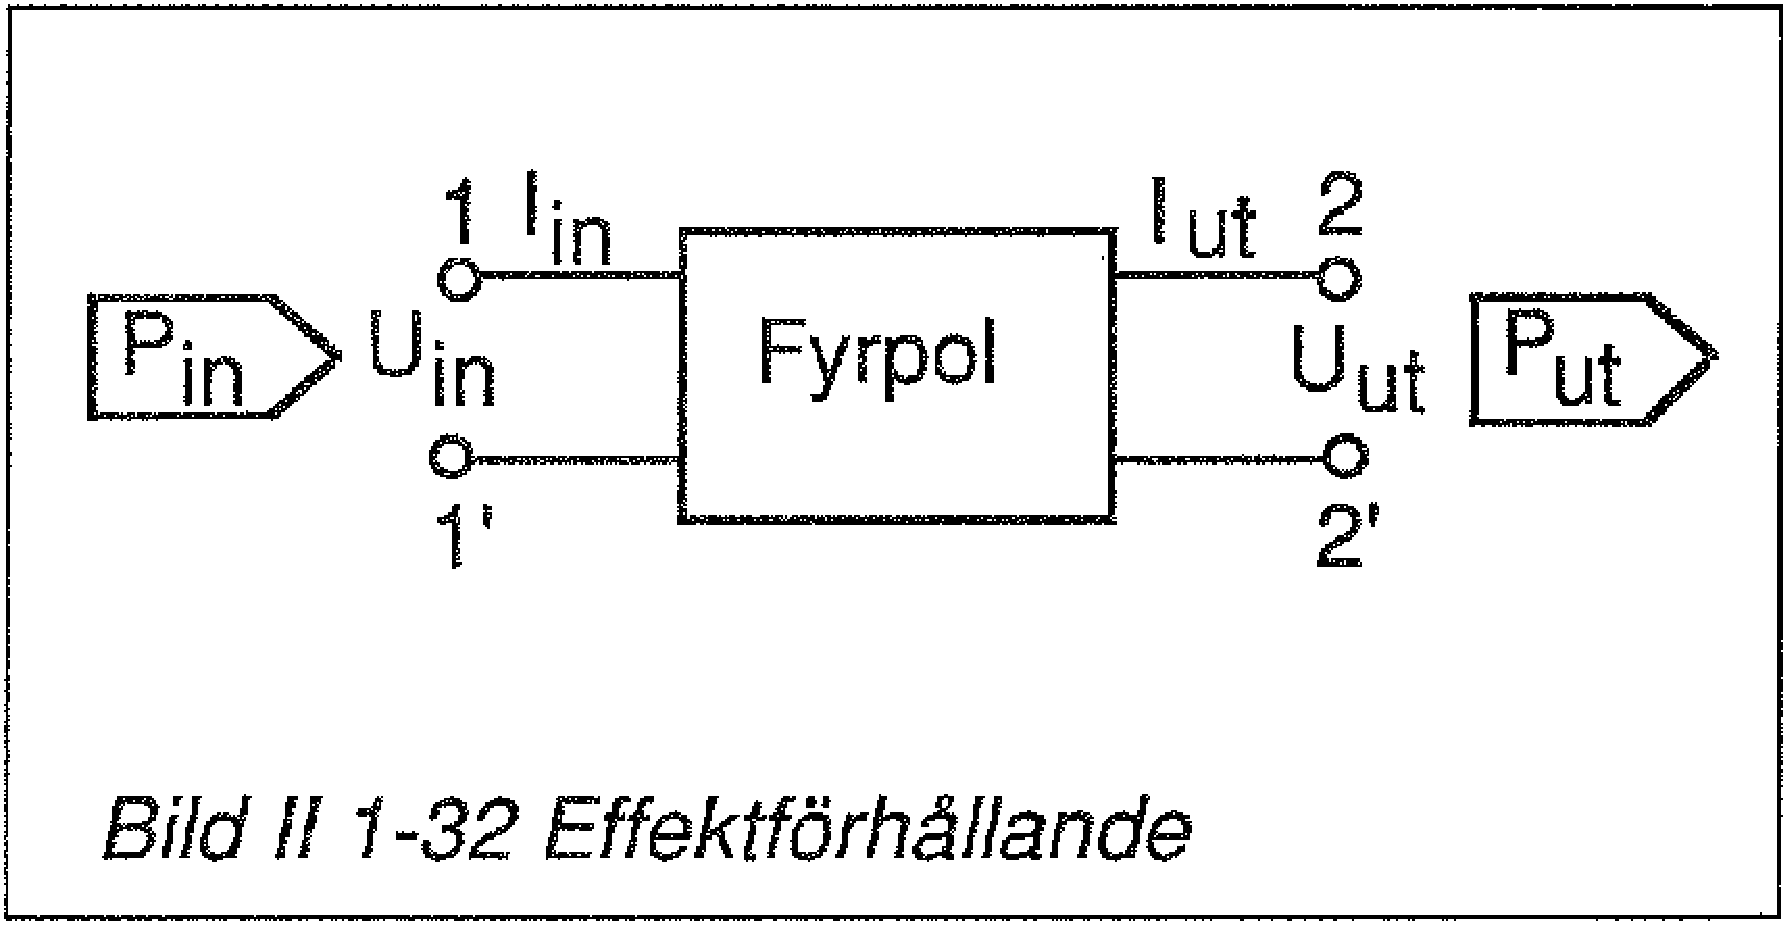
\includegraphics[width=7cm]{images/bild_2_1-32}
\caption{Effektförhållande}
\label{fig:BildII1-32}
\end{center}
\end{figure}

Antag att den inmatade effekten P är 1 W. Om effekten inte ändras vid passagen
genom fyrpolen, så är även den uttagna effekten 1 W.

\emph{Effektförhållandet} mellan in- och utgångarna är då

\(\dfrac{P_{in}}{P_{ut}} = \dfrac{1\ watt}{1\ watt} = 1 (kvoten = 1)\)

Oförändrad effekt varken dämpas eller förstärks, varför både dämpningen och
förstärkningen har talvärdet 0. Enheten på talvärdet är Bel, dämpningen eller
förstärkningen är således 0 Bel. En tiondel därav är 0~decibel (0 dB).

Omräkning av kvoten av en effektändring till dB görs så, att 10-logaritmen för
kvoten söks och resultatet blir effektändringen uttryckt i Bel (B). Om
resultatet uttrycks i dB, ska Bel-värdet multipliceras med 10.

Logaritmer förklaras i appendix \ref{logaritmer}.

För att förenkla beräkningen av dB-talet divideras det högre effekttalet med det
lägre. Bokstaven a i följande formler betyder antingen förstärkning (+a) eller
dämpning (-a) beroendet på vilket förtecken som sätts.

\(a[B] = \log \dfrac{P_\text{hög}}{P_\text{låg}}\)

\(a[dB] = 10\log \dfrac{P_\text{hög}}{P_\text{låg}}\)

Att addera eller subtrahera värden på en logaritmisk skala, motsvarar att
multiplicera resp. dividera värden på en linjär skala. Huvudskalorna på en
räknesticka är logaritmiska. (Räknestickan är ett enkelt, förut mycket använt
hjälpmedel).

Med hjälp av nomogrammet i bild \ref{ellära-nomogram-db-effekt} kan en \textbf{effektändring}, uttryckt som kvot
(effekterna dividerade med varandra), omvandlas till decibel och omvänt.

\begin{figure}
  \fbox{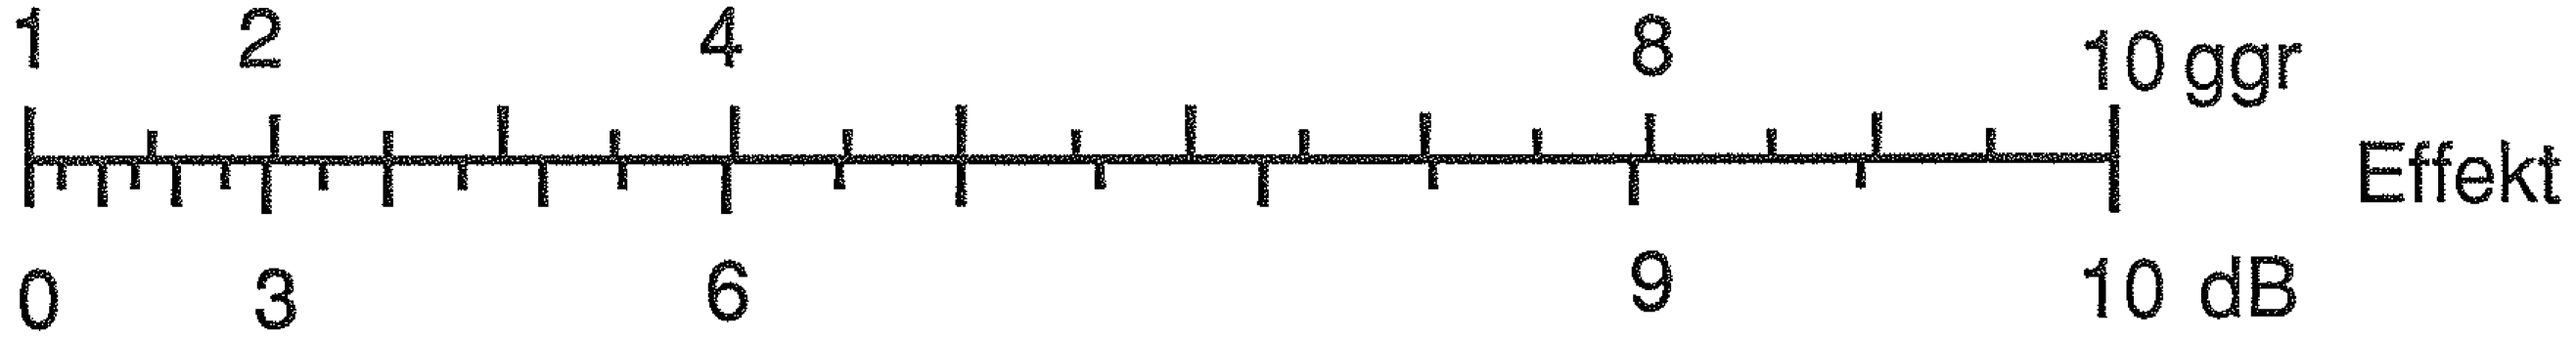
\includegraphics[width=\textwidth]{images/nomogram_db_effekt}}
  \caption{Nomogram för omvandling mellan effekt och decibel}
  \label{ellära-nomogram-db-effekt}
\end{figure}

Följande avrundade värden kan utläsas:

\begin{tabular}{rlrlrl}
0 dB & = 1 &  1 dB & =  1,25 & 2 dB = 1,6 \\
3 dB & = 2 &  4 dB & =  2,5  & 5 dB = 3,2 \\
6 dB & = 4 &  7 dB & =  5    & 8 dB = 6,3 \\
9 dB & = 8 & 10 dB & = 10    & 11 dB = 12,5
\end{tabular}

\begin{quote}\emph{
d.v.s. vid ökning fördubblas effekten för var 3:e dB och vid minskning
halveras effekten för var 3:e dB.
}\end{quote}

Om kvoten är en eller flera 10-potenser högre än 10, så kan nomogrammet utökas
enligt följande tabell.

\begin{tabular}{rllr}
Kvot av & Analys             & Skriv            & dB \\
\(P_\text{hög}/P_\text{låg}\) &          &                  &    \\
     1 & 1 har 0 nollor      & \(0 \cdot 10\) = &  0 \\
    10 & 10 har 1 nolla      & \(1 \cdot 10\) = & 10 \\
   100 & 100 har 2 nollor    & \(2 \cdot 10\) = & 20 \\
 1 000 &  1 000 har 3 nollor & \(3 \cdot 10\) = & 30 \\
10 000 & 10 000 har 4 nollor & \(4 \cdot 10\) = & 40
\end{tabular}

\subsection{Strömändring uttryckt i dB}
\index{ström!dB}
\index{dB!ström}

Förhållandet mellan strömmar liksom mellan spänningar kan även uttryckas i dB,
men annorlunda än mellan effekter. En fyrpol med inbördes lika ingångs- och utgångsimpedans är förutsättningen för jämförelse.

Enligt Joules lag är \(P = I^2 \cdot R\) (\(P = U \cdot I\))

således \(\dfrac{P_\text{h{\oe}g}}{P_\text{l{\aa}g}} = \dfrac{I_\text{hög}^2 \cdot R}{I_\text{l{\aa}g}^2 \cdot R}\)

R kan avkortas \emph{om in- och utgångsimpedanserna (resistanserna) är lika}.

En jämförelse uttryckt i dB kan endast göras
under samma förutsättningar; här att impedanserna (resistanserna) är lika,

således \(\dfrac{P_\text{hög}}{P_\text{låg}} = \dfrac{I_\text{hög}^2}{I_\text{låg}^2}\)

Effektförhållandet eller kvadratvärdet på
strömförhållandet kan uttryckas logaritmiskt
i B eller dB

\(a[dB] = 10\log \dfrac{I_\text{hög}^2}{I_\text{låg}^2}\)

Eftersom \(\log x^2 = 2 \cdot \log x\), fås slutligen

\(a[dB] = 20\log \dfrac{I_\text{hög}}{I_\text{låg}}\)

\subsection{Spänningsändring uttryckt i dB}
\index{spänning!dB}
\index{dB!spänning}

Förhållandet mellan spänningar kan uttryckas i dB på ett liknande sätt som med
strömmar.

Enligt Joules lag är \(P = \frac{U^2}{R}\) (\(P = U \cdot I\))

Två effekter kan ställas i förhållande till varandra på följande sätt:

\(\dfrac{P_\text{hög}}{P_\text{låg}}=\dfrac{U_\text{hög}^2 \cdot R}{U_\text{låg}^2 \cdot R}\)

R avkortas och efter omskrivning fås en formel som liknar den för strömmar

\(\dfrac{P_\text{hög}}{P_\text{låg}} = \dfrac{U_\text{hög}^2}{U_\text{låg}^2}\)

\(a[dB] = 20\log \dfrac{U_\text{hög}}{U_\text{låg}}\)

Med nomogrammet i bild \ref{ellära-nomogram-db-spänning} kan kvoten av en ström- eller spänningsändring omvandlas
till decibel och tvärt om.

\begin{figure}
  \fbox{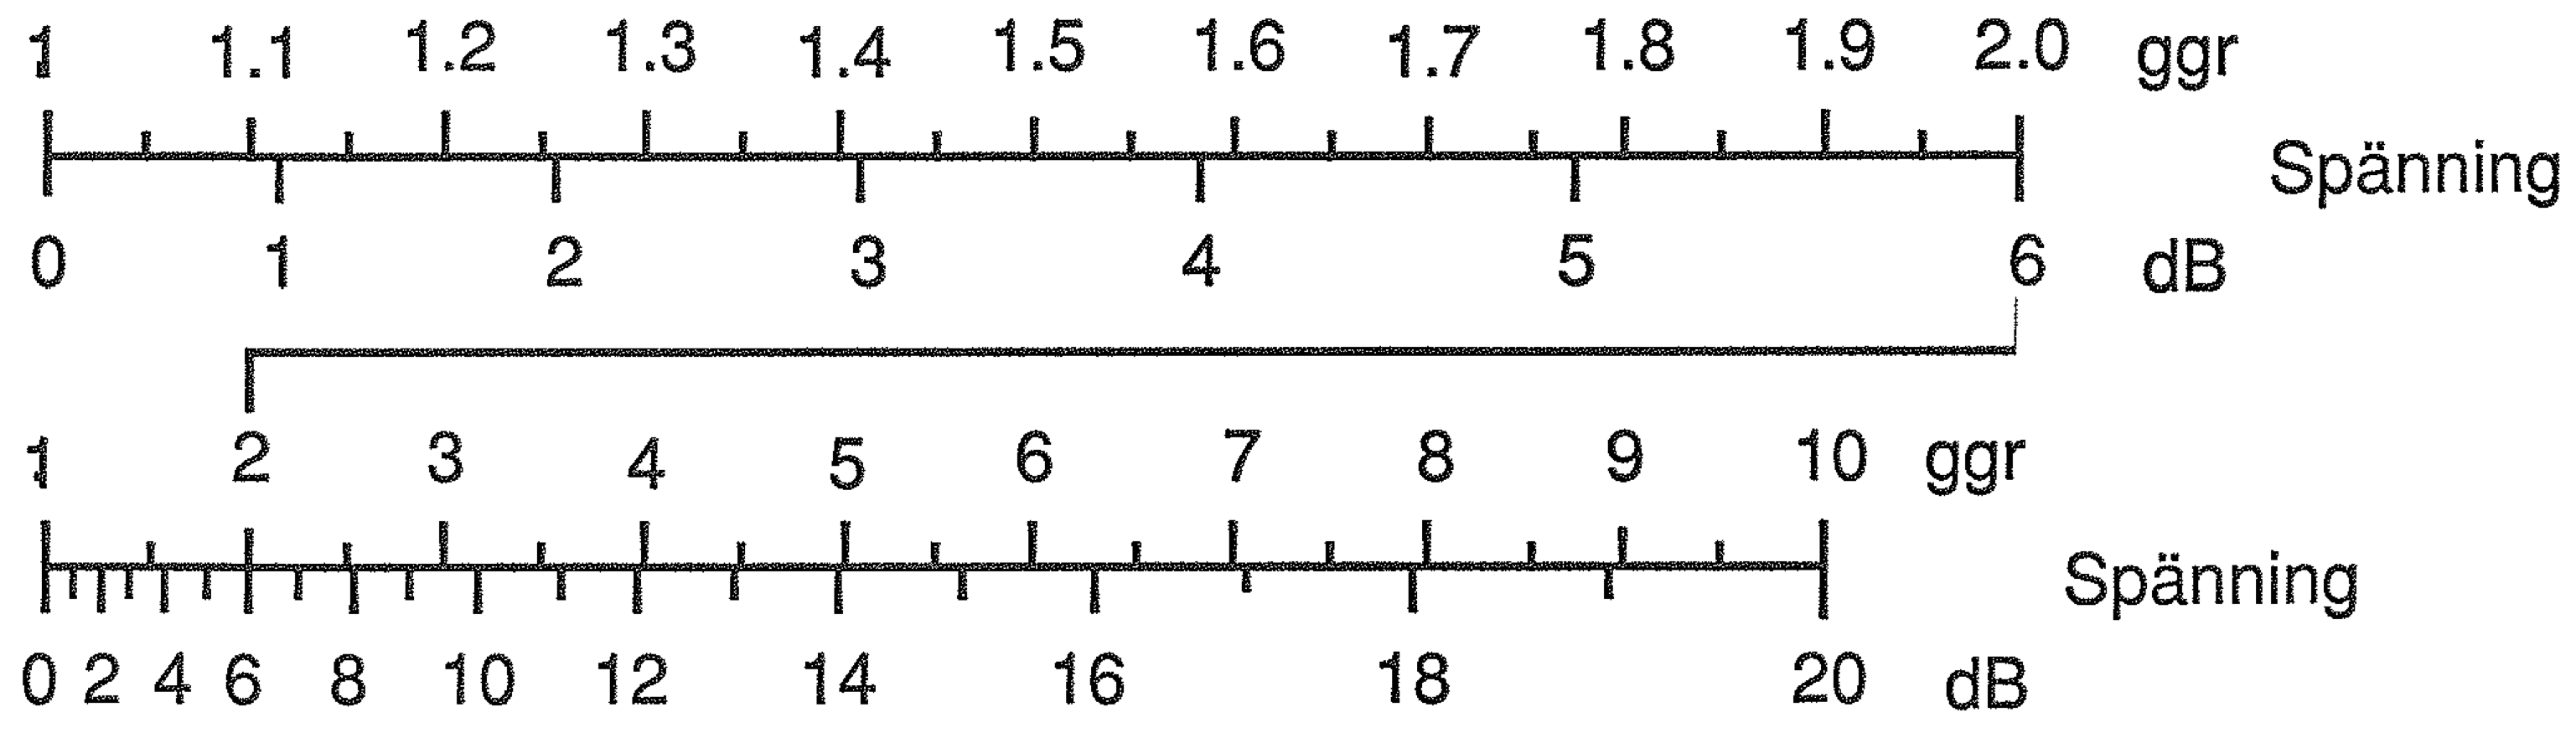
\includegraphics[width=\textwidth]{images/nomogram_db_spanning}}
  \caption{Nomogram för omvandling mellan spänning och decibel}
  \label{ellära-nomogram-db-spänning}
\end{figure}

Följande avrundade värden kan utläsas:

\begin{tabular}{rlrlrl}
0 dB & = 1   &  1 dB & = 1,12 &  2 dB = 1,25 \\
3 dB & = 1,4 &  4 dB & = 1,6  &  5 dB = 1,8 \\
6 dB & = 2   &  7 dB & = 2,24 &  8 dB = 2,5 \\
9 dB & = 2,8 & 10 dB & = 3,2  & 11 dB = 3,6
\end{tabular}

\begin{quote}\emph{
d. v. s. vid ökning fördubblas strömmen resp. spänningen för var 6:e dB och att
vid minskning halveras strömmen resp. spänningen för var 6:e dB.
}\end{quote}

Om kvoten är en eller flera 10-potenser högre än 10, så kan nomogrammet utökas
enligt följande tabell.

\begin{tabular}{rllr}
Kvot av & Analys             & Skriv            & dB \\
\(U_\text{hög}/U_\text{låg}\) &          &                  &    \\
\(I_\text{hög}/I_\text{låg}\) &          &                  &    \\
     1 & 1 har 0 nollor      & \(0 \cdot 20\) = &  0 \\
    10 & 10 har 1 nolla      & \(1 \cdot 20\) = & 20 \\
   100 & 100 har 2 nollor    & \(2 \cdot 20\) = & 40 \\
 1 000 &  1 000 har 3 nollor & \(3 \cdot 20\) = & 60 \\
10 000 & 10 000 har 4 nollor & \(4 \cdot 20\) = & 80
\end{tabular}

Se appendix \ref{decibel} för beräkning med tabeller.

\subsection{Ändring uttryckt i dB vid förstärkande eller dämpande anordningar kopplade i serie}
\textbf{HAREC a.\ref{HAREC.a.1.9.3}\label{myHAREC.a.1.9.3}}

Ett räkneexempel på effektändringar:
Fråga:
Vi har en enkel sändaranläggning med ett drivsteg med en in effekt av 10 W.
Drivsteget förstärker med 6 dB. Vidare har vi ett effektslutsteg som förstärker
med 10 dB. Antennkabeln dämpar med 1 dB.

Med vilken effekt matas själva antennen?

Svar: (två sätt att lösa uppgiften)
\begin{enumerate}
\item Drivsteget förstärker fyra gånger, slutsteget förstärker tio gånger och
kabeln dämpar \(1/1,25 = 0,8\) gånger. Antennen matas då med
\(10 \cdot 4 \cdot 10 \cdot 0,8 = 320\ W\).
\item Drivstegets 6 dB plus slutstegets 10 dB minus antennkabelns 1 dB = 15 dB.
15 dB är \(10 + 5\ dB\) d.v.s. \(10 \cdot 3,2 = 32\ ggr\). Antennen matas med
\(10\ W \cdot 32 = 320\ W\).
\end{enumerate}

\subsection{Impedansanpassning}
\textbf{HAREC a.\ref{HAREC.a.1.9.4}\label{myHAREC.a.1.9.4}}
\index{impedansanpassning}
\index{impedans!anpassning}

Impedansanpassning är av stor betydelse inom kommunikationstekniken.
Normalt vill man nämligen överföra mesta möjliga effekt från energikällan
(t.ex. sändaren) till förbrukaren (t.ex. antennen).

Varje spänningskälla har en inre resistans \(R_i\). Det innebär som först att
källan inte kan avge oändligt stor ström. För att förenkla det hela antar vi nu
att en sändare med den inre resistansen \(R_i\) ansluts direkt till en antenn
med resistansen \(R_a\).

Målet med anpassningen är att finna det optimala förhållandet mellan
sändarresistansen och antennresistansen för att kunna överföra maximal effekt.
Vi har de två ytterlighetsfallen obelastad sändare respektive kortsluten
sändare. Sändarens elektromotoriska kraft (EMK) betecknas som \(E\ [V]\) och
sändarens utspänning som \(U\ [V]\).

Fall 1.
En obelastad sändare avger ingen ström när ingen antenn eller en med oändligt
stor resistans har anslutits.
Alltså vid obelastad sändare:

\(
\begin{array}{lllll}
R_a = \infty & & I = 0 & & U = E
\end{array}
\)

Fall 2.
När sändarutgången är kortsluten, d.v.s. belastningen (antennresistansen) är
noll ohm, avger sändaren en ström som beror av EMK och inre resistans. Eftersom
sändarutgången är kortsluten är utspänningen \(U\) noll.
Alltså vid kortsluten sändare:

\(
\begin{array}{lllll}
R_a = 0 & & I = \dfrac{E}{R_i} & & U = O
\end{array}
\)

I båda ytterlighetsfallen är den effekt som omsätts i \(R_a\) lika med noll.
För att få ut någon effekt måste man alltså söka ett värde på \(R_a\) som
ligger mellan ytterlighetsvärdena.

Enligt formeln för spänningsdelare är utspänningen

\(U = E \cdot \dfrac{R_a}{R_a+R_i}\)

Formeln för uteffektens effektivvärde är

\(P_{ut} = \dfrac{U^2}{R_a}\)

Efter insättning får man

\(P_{ut} = \dfrac{E^2 \cdot R_a}{(R_a + R_i)^2}\)

För att finna det optimala förhållandet mellan \(R_i\) och \(R_a\), d.v.s. när
\(R_a\) tar upp maximal effekt, måste man differentiera formeln med \(d\ P_a/d\ R_a\), men vi hoppar över denna utflykt i matematiken.

I stället konstaterar vi helt enkelt att \emph{maximal effektöverföring sker när
\(R_i = R_a\)}.

\subsection{Förhållandet mellan in- och uteffekt uttryckt som \% verkningsgrad}
\textbf{HAREC a.\ref{HAREC.a.1.9.5}\label{myHAREC.a.1.9.5}}
\index{verkningsgrad}

Antag att en antennkabel har en effektförlust av 1~dB. Det innebär en
effektdämpning av 1,25 gånger, d.v.s. 0,8. Nu matar vi in 10~W i kabeln och får
alltså ut 8~W. Hur stor verkningsgrad har kabeln uttryckt i \% ?
Lösning:

\(\eta = \frac{8}{10} \cdot 100 = 80\ \%\)

\subsection{Toppvärdeseffekt P.E.P.}
\textbf{HAREC a.\ref{HAREC.a.1.9.6}\label{myHAREC.a.1.9.6}}
\index{toppvärdeseffekt}
\index{effekt!toppvärdes}
\index{P.E.P.}
\index{effekt!P.E.P.}

Uteffekten från en sändare kan mätas över en konstlast (dummy load). En
konstlast är en resistor som kan omsätta sändarens hela effekt till värme. Med
HF-mätprob och en detektordiod eller en HF-voltmeter kan man mäta
effektivvärdet på spänningen över konstlasten och beräkna uteffekten med
formeln

\(P_{ut} = \frac{U^2}{R}\)

U = HF-spänningens effektivvärde
R = resistansen i konstlasten

På grund av utsignalens karaktär kan man inte mäta effektivvärdet av uteffekten
från SSB-sändare. Med oscilloskop kan man emellertid mäta utspänningen på den
största modulationstoppen.

Med detta toppvärde kan man beräkna spänningen över konstlasten.

Uteffekten definierad som P.E.P. (Peak Envelope Power) är ''den medeleffekt som
matas in i en antennmatarledning under det högsta effektvärdet inom en
frekvenscykel och mätt under normal drift''.

\(P.E.P. = \dfrac{\hat{u}^2}{R}\)

där \(\hat{u}\) är momentanspänningen på den största modulationstoppen.



%\chapter{KOMPONENTER}

\section{Resistorn}

Allmänt

Strömkretsar består av komponenter med
olika egenskaper. Den vanligaste egenskapen, åtminstone i likströmskretsar, är resistansen. För att få avsedd funktion, så anpassar man resistansen i komponenterna.
Exempel
En krets med strömkälla, lampa, kopplingsledningar och smältsäkring. Kopplingsledningarna mellan komponenterna bör ha
låg resistans och därför lågt spänningsfall
(små förluster). Lampan skall däremot ha
hög resistans och därmed höga förluster för
att kunna bli het och lysa. Smältsäkringen
skall skydda ledningarna från för hög ström.
Säkringen ges därför en resistans, som gör
att den smälter när strömmen överstiger ett
tillåtet värde.
Som hjälpmedel för att fördela spänningar
och strömmar i en krets, så används en
komponenttyp kallad resistor. Dess utmärkande egenskap är resistans- även kallad
ohmskt motstånd.

Enheten Ohm

(Se även kapitel 1)
Resistansen mellan två punkter i en strömkrets är 1 n (uttalas "en åm"), när spänningen mellan punkterna gör att en ström av
1 A (en ampere) flyter i kretsen.
Inom elektroniken används höga resistansvärden och därför även följande multipler av enheten
3
(1 kn) == 106 Ohm
1 kiloohm
1 mego hm
(1 Mn) == 10 Ohm

Resistans i strömledare

För att bestämma resistansen, t. ex. i en tråd,
behöver man veta dess resistivitet, tvärsnittsyta, längd och temperatur.

Resistivitet
Resistivitet är ett materials strömledningsegenskaper. Ett annat namn för resistivitet
är specifik resistans. Symbolen för resistivitet
är p (uttalas rå).

..
. . . ..
ohm ·mm 2
Form e ln for res1St1v1tet ar p =- - - m
Följande formel gäller för beräkning av
resistansen i en strömledare med linjär ström/spänningskaraktär.

R= p!

A

![meter] A [mm

2

]

[p= n·A]
m

Exempel
l = 4 m koppartråd
A== 2 mm 2
p (koppar) == 0.017

l
A

R=p-

R=0.017i=o.034 n
2

Not. Förväxla inte A [tvärsnittsytan] i denna
formel med beteckningen A t. ex. i Ohms lag då A
betecknar strömstyrkan.

Resistiva material

Resistorer kan utföras med olika typer av
resistiva material, vilket bestämmer användningsområdet.
En resistor, vars resistans är oberoende
av ström, spänning och annan yttre påverkan t.ex. temperatur och ljus, sägs ha linjär
karaktär. Om resistansen däremot beror av
yttre påverkan, så sägs resistorn ha olinjär
karaktär.
Man skiljer mellan tre huvudgrupper av
resistiva material. Det kan vara en kropp av
pressat kol eller ett ledande ytskikt på ett
isolerande underlag eller metalltråd på en
isolerande stomme. På senare tid har tillkommit integrerade resistorer, d.v.s. flera
resistorer av resistiva skikt på ett gemensamt isolerande underlag. Här beskrivs i
korthet
resistortyper. Se f.ö. leverantörskataloger.

Utförandeformer

Resistorer kan utföras med fast eller ställbart resistansvärde. Här följer först en översikt över resistorer med olika resistiva material och fast resistansvärde.

112-1

K MP NENTER
Fasta resistorer med linjär karaktär
Massaresistar
Det resistiva materialet består av kolmassa
med bindemedel (kolkomposit). Massan är
bakad till en stav eller ett rör. Anslutningsledningarna är inbakade i materialet.
Massaresistorer är lämpliga för lik- och
växelströmskretsar med låga krav på temperaturberoende och egenbrus. Den homogena kroppen gör att egeninduktansen är
låg. Å andra sidan uppstår vid höga frekvenser en skineffekt, d.v.s. strömkoncentration
vid ytan, som medför viss resistansökning.
Kolfilmsresistor
Det resistiva materialet består av ett kolskikt,
som genom förångning överförts till ett keramiskt rör. Resistansen bestäms av tjockleken på skiktet samt av spiralformade spår i
detta. Genom spiraliseringen tillförs en induktans, men som i någon mån uppvägs av
egenkapacitansen.
Metallfilmresistor
l denna typ är kolfilmen ersatt av ett metallskikt. Eftersom egenkapacitansen är liten,
så är typen lämpad för höga frekvenser.
Tjockfilmsresistor
Det resistiva materialet består en film av bl. a.
metalloxid, som screentrycks på ett keramiskt underlag. Typen har god tålighet mot
pulser och höga temperaturer, men har relativt högt egenbrus. Ytmonterade resistorer
är oftast tillverkade av tjockfilm.
Tunnfilmsresistor
Det resistiva materialet består av en tunn
metallfilm, som genom förångning överförts
till ett underlag av glas eller keramik.
Denna resistertyp har över lag god stabilitet och används ofta i apparater med hög
precision. Egenskaperna vid höga frekvenser är dock inte så bra.
Metalloxidresistor
Denna resistertyp har ett spiralformat skikt
av metalloxid. Temperatur- och spänningsberoendet är måttligt. Tåligheten mot pulser
och höga temperaturer är stor. Typen kan i
någon mån ersätta trådlindade resistorer.

112-2

Resistarnät
Resisternät (integrerade resistorer) består
av flera resistiva skikt på ett gemensamt
isolerande underlag, d.v.s. liknande teknik
som för tjock-och tunnfilmsresistorer.
Trådlindad resistor
Det resistiva materialet är en metalltråd,
som är lindad på en stomme som tål hög
temperatur; det kan var keramik, glas etc.
Tåligheten mot pulser och höga temperaturer är stor.

Fasta resistm·er med olinjär karaktär
Vanligast är att materialet i resistorer har
linjär ström-/spänningskaraktär, men det
finns även sådana med olinjär karaktär. l
resistorer med olinjär karaktär är det ingående materialet av halvledartyp.
Spänningsberoende resistor
- Voltage Dependent Resistar (VOR)
Linjära resistorer påverkas knappast av den
pålagda spänningen. Resistorer av kiselkarbid har däremot en hög resistans vid låg
spänning och omvänt en låg resistans vid
hög spänning. VOR används t.ex. för begränsning av spänningstoppar.
Ljusberoende resistor, fotoresistor
- Light Dependent Resistar (LDR)
Ledningsförmågan i halvledare påverkas inte
bara av värme utan även av ljus. Halvledare
av germanium och särskilt sammansatta
halvledare av kadmiumoxid, blysulfid och
indiumantimonid har särskilt stor ljuskänslighet. Kadmiumsulfid är känsligast för synligt ljus medan andra material är känsligast i
det infraröda området.
Magnetfältberoende resistor (fältplatta)
Resistansen ökar med längden på strömledaren. Denna egenskap används i magnetfältberoende fältplattor. En sådan består
av en keramisk bärarplatta med en yta av
indiumantimon id. l ytan är ytterst smala parallella metallbanor inlagda på ett avstånd av
någon J.lm. Normalt går strömmen kortaste
vägen tvärs över banorna, men när ett magnetfält träffar vinkelrätt mot plattans yta, så

K MP NENTER
avlänkas elektronerna. De får då längre väg
över till nästa metallbana och den totala
resistansen ökar.

Temperaturberoende resistor

Se nedan om NTC och PTC i resistorer.

Temperaturkoefficienten för resistorer
Resistansen i ingående material påverkas
av temperaturen, vaNid det skiljer mellan
materialen.
Amorft kol och de flesta halvledande
materialleder bättre när de är varma- de har
en negativ temperaturkoefficient (NTC). Sådana material finns t. ex. i dioder och transistorer.
Däremot leder metaller och speciella
halvledarmaterial bättre när de är kalla- de
har en positiv temperaturkoefficient (PTC).
Glödtråden i glödlampor och elektronrör är
resistorer med positiv temperaturkoefficient
(PTC). l vissa metallegeringar, som t.ex. i
konstantan, kan resistansen till och med
vara nästan konstant vid varierande temperatur.
Alla material har en temperaturkoefficient,
som anger hur mycket resistansen ändras
per grad. Resistansen vid någon annan temperatur kan därför beräknas med följande
formel, där man sätter in begynnelsetemperaturen [ o] (o c), temperaturändringen [ .1.0]
och temperaturkoefficienten [a].

Rvarm= Rkall$\pm$ a· il ?J· Rkatt
Resistansändringen är ledet
AR= $\pm$a· .1.19- ·Rkatt
Temperaturkoefficienten kan vara positiv (NTC) eller negativ (NTC).
l principscheman har PTC- respektive NTCresistorer symboler som på bilden.
Bild nr 112-1

Variabla resistorer
En resister kan även utföras med variabelt
resistansvärde. Då används endast den andel av det resistiva materialet, som finns
mellan en resistors ena ände och ett uttag
någonstans mellan ändarna. En sådan anordning kallas för reostat. Om en variabel
resister används som spänningsdelare, så
kallas den för potentiometer.

l en potentiometer används dels hela
resistansen mellan ändpunkterna och dels
andelen mellan uttaget och någon av
ändpunkterna.
Uttagets mekaniska utförande beror oftast av hur bekvämt inställningen skall kunna
ske. En potentiometer, där det resistiva
materialet är lagt på en cirkulär bana och
uttaget är fäst vid en axel i banans centrum,
medger enkel inställning med mejsel, ratt
etc. Ett enklare slags uttag är en släpkontakt
eller ett spännband som kan flyttas utmed en
stavformad resistor.

Resistiva material i variabla resistorer

Banan i en variabel resister består i princip
av liknande resistiva material som i en fast
resistor.
Billigast och enklast är en bana av kol,
som är tryck på ett enkelt underlag. Nackdelar är låg efekttålighet, dålig upplösning och
linjäritet, högt brus och kort livslängd. Fördelen är lågt pris.
Bättre än en kolbana är en bana av kolkomposit, d.v.s. kolpulver med bindemedel,
som är tryckt på ett underlag. Nackdel är
högre pris och låg effekttålighet, medan fördelarna är god upplösning, lågt brus och
lång livslängd.
Vill man ha god effekttålighet och temperaturstabilitet, utöver kolkompositens egenskaper, så erbjuder en bana av cermetsådana fördelar. En cermetbana består av en
blandning av metaller och keramik, som
trycks på ett underlag.
Trådlindad bana har främst god tålighet
mot hög effekt. Tålighet vid hög ström genom uttaget är en nannan fördel.

Linjära och olinjära patentiometrar

En potentiometer har en kuNform, varvid
avses resistansändringen som funktion av
uttagets rörelseväg utmed resistansbanan.
KuNformen kan utföras linjär, logaritmisk
etc .. Olinjära kuNor består då oftast av en
följd av linjära segment, som tillsammans
någorlunda motsvarar den önskade olinjära
formen. Ett exempel på det är när en kurvform
anges som linjär/logaritmisk.

112-3

K MP N
Effektutveckling i resistorer
l resistorer utvecklas värme av den ström
som flyter igenom. Värmeutvecklingen sker
enligt Joule's lag, som återges i kapitel1.
Hur mycket effekt i form av värme som
strålas ut från resistorn beror på storleken på
dess yta och egentemperatur samt på omgivningens temperatur. Det finns en övre
gräns för hur stor värme det ingående materialet tål innan det förstörs och eventuellt
fattar eld.
En resistors effekttålighet framgår i vissa
fall av påstämplade värden. l övriga fall är
man hänvisad till kataloguppgifter eller en
bedömning, som ev. kan grundas på höljets
utseende och dimensioner.
standardiserade komponentvärden
Resistorer tillverkas vanligen med standardiserade värden ur någon talserie.
Märkning av resistorer
Resistorer märkas med huvuddata enligt
något system av siffror och bokstäver eller
med en färgkod. Flera olika system tillämpas.
(Se f.ö. leverantörskatalogerför information
om komponentdata, märkning o.s.v.)

2

1
2
3
4

3

4

Allmän symbol
ställbar resistor, potentiometer
Trimbar resister (trimmer)
Automatiskt ställbar resister

Bild 112-1 Schemasymboler för resistorer

112-4

5

5
6
7
8

6

7

Temperaturberoende resistor,
Temperaturberoende resistor,
Spänningsberoende resistor,
Ljusberoende resistor,

8

NTC
PTC
VOR
LDR

K MP NENTER

2.2 Kondensatorn
Allmänt

Följande formler gäller för kapacitansen i
en enkel kondensator med två plattor. När
en kondensator är uppbyggd av n stycken
plattor, ökar kapacitansen med faktorn (n-1 ).
Med vakuum som dielektrikum gäller

Så snart det finns en elektrisk potentialskillnad .,..-en spänning - mellan två kroppar, så
uppstår ett elektriskt kraftfält mellan dem.
Ett sådant fält är lagrad elektrisk energi.
Kropparna måste då isoleras från varandra.
Elektrisk energi lagras mellan olika delar
av en strömkrets, även om de inte är direkt
avsedda för det. Särskilt vid mycket höga
frekvenser har detta stor betydelse för utformningen av en strömkrets. Vid låga frekvenser och likström däremot, har kretsens
utformning mindre inverkan. Då behövs i
stället särskilda anordningar för ta upp eller
avge energi på önskade ställen i strömkretsen.
En sådan anordning kallas kondensator.
Den består i princip av två band eller plattor
med anslutningsledningar samt ett isolerande skikt- dielektricum- däremellan.
Kapacitansen är näst efter resistansen
den vanligaste egenskapen i en strömkrets.

Kapacitans är elektricitetsmängden per volt
där måttenheten är Farad [F]. Eftersom denna
enhet är mycket stor, används inom elektroniken oftast bråkdelar av den.
1 mikrofarad (1 !-!F) = 1o-6 F
1 nanofarad (1 n F) = 1 9 F
1 pikofarad (1 p F) = 1o- 12 F

Kapacitans

Kondensatorn i likströmskretsen

Förmågan att lagra elektrisk energi (elektrisk laddning) kallas kapacitans. Ordet kommer från latinets capax, som betyder rymlig,
duglig.
Kapacitansen betecknas i formler med
bokstaven C
•
•
•
•

En kondensators kapacitans bestäms av
ytan på kondensatorns plattor,
avståndet mellan dessa ytor,
den absolutadielektricitetskonstanten c0
den relativa dielektricitetskonstanten
som är den faktor kapacitansen ökar med
när dielektrikum är annat än vakuum.

c,;

Kapacitans, dimension och dielektrikum

Kapacitansen är proportionell med den yta,
som kondensatorplattorna skuggar varandra, och är omvänt proportionell med plattavståndet.

1•

A

C=cod

Med ett godtyckligt dielektrikum gäller

2.
C [Farad]

d [mm]

E [F/m]

Enheten Farad

o-

En kondensator i en likströmskrets har alltid
samma polaritet. Därvid förhåller sig kondensatorns polspänning till dess laddningsmängd.
En ström flyter till kondensatorn och laddar upp den, när den anslutna spänningskällan har högre spänning än kondensatorn. Ju
högre spänningen är, desto större är laddningen. Ju kortare uppladdningstiden är, desto högre effekt utvecklas under den tiden.
När en uppladdad kondensator ansluts
till en krets med lägre spänning, så urladdas
kondensatorn till kretsen. Ju kortare urladdningstiden är, desto högre effekt utvecklas
under den tiden.
Laddningen i en kondensator kan innebära hög polspänning. Om kondensatorns
kapacitet är stor, kan laddningsmängden bli
betydande. Varning för elektriska stötar och
brännskador!

112-5

K
Kondensatorn i växelströmskretsen
l en likströmskrets förhåller sig kondensatorns polspänning till laddningsmängden. l
en växelströmskrets växlar emelltid spänningen och polariteten ständigt och därmed
kondensatorns laddning och polaritet.
Not: Vissa kondensatortyper kan inte användas i rena växelströmskretsar.
Försök
En glödlampa och en kondensator kopplas i
serie med varandra och ansluts till en
växelströmskrets. Med lämpligt valda värden på komponenterna kommer lampan att
lysa upp.
Detta visar att en kondensator inte hindrar elektronflödet i en växelström krets. Man
brukar säga att kondensatorn "släpper igenom växelström", men i stället är det så att
laddningar pendlar mellan kondensatorns
plattor genom den strömkrets som kondensatorn är ansluten till.
Använd för säkerhets skulllåg spänning,
t.ex. den från en ringledningstransformator!

Kapacitiv reaktans
Strömstyrkan i en växelströmskrets beror
bl.a. på hur stor kondensatorns kapacitans
är, d.v.s. på dess kapacitiva reaklans Xc.
Ordet reaktans kommer från latinets re
(åter) agere (verka).
Större kapacitans innebär större förmåga att ta upp elektrisk laddning och ger
därmed en lägre reaktans. Resultatet blir ett
kraftigare elektronflöde. En mindre kapacitans innebär ett svagare elektronflöde.

1
2n:fC

Xc=-- eller

1
mC

Xc=-

[O]
[Hz]
[F]
eller
[MO]
[MHz]
[uF]
(samma sortenheter i alla led)
Exempel:

f = 50 Hz
1
1
xc -- 2 n:fC - 2 n 50 ·1 O·1

1.

2.

112-6

C = 1O J.tF

c = 1oJ.tF

Xc = ?
=318.3 Q

XC = ?

En kondensators reaktans är således
omvänt proportionell med dess kapacitans
och frekvensen i kretsen.
Jämför detta med en induktor där reaktansen är proportionell med frekvensen.
När en ström flyter genom en res istor, så
uppstår det värmeförluster. När ström flyter
genom en ideal reaktans- en induktor eller
en kondensator - uppstår däremot inga
värmeförluster.

Fasförskjutning i en kondensator
Med fasförskjutning menas här den tidsmässiga förskjutningen mellan ström- och
spänningsförloppen. l en kondensator når
nämligen strömmen inte sitt toppvärde samtidigt som spänningen. l en ideal kondensator är spänningen fasförskjuten 90$\circ$ efter
strömmen.
Förlustvinkel
l praktiken är fasförskjutningen i en kondensator något mindre än 90$\circ$ på grund av att
laddning läcker igenom dielektrikum. Man
talar om en förlustvinkeL Läckningen kan
ses som en resister som är kopplad parallellt
över kondensatorn.
läckström m.m.
Med det extremt tunna. dielektrikum har
elektolytkondensatorn en mycket högre kapacitet än andra former, men har också
några nackdelar, bl.a. att
• den normalt endast kan användas med
likspänning,
• den har hög förlustfaktor p.g.a.läckström,
• det utvecklas värme av läckströmmen,
vilket skapar övertryck p.g.a. gasbildning.
Utförandeformer
Kondensatorer kan utföras med fast kapacitansvärde. Dielektrikum består då av ett
skikt av glimmer, impregnerat papper o.s.v.
Kondensatorer kan även utföras med variabelt kapacitansvärde. Dielektrikum består
då oftast av luft, men kan även vara ett fast
material.

Fasta kondensatorer
Kondensatorer har oftast namn efter utförande och materialet i dielektrikum
Pappers- och plastkondensatorer
'Plattorna" i dessa typer består av aluminiumremsor med anslutningstrådaL Däremellan finns en pappers- respektive plastremsa
som dielektrikum. För att spara plats, så
rullas det hela ihop och skyddas med en
plastingjutning.
Keramiska kondensatorer
l keramiska kondensatorer består dielektrikum av något keramiskt material. På ömse
sidor om detta sätts en metallbeläggning
med anslutningstrådaL
Glimmerkondensatorer
l denna kondensatortyp består dielektrikum
av tunna glimmerskivor
Elektrolytkondensatorer
Elektrolytkondensatorer har elektroder av
aluminium eller tantal, därpluspolen (anoden)
ges ett mycket tunt oxidskikt Detta är inte
ledande och fungerarsom dielektrikum. Mellan oxidskiktet och minuspolen (katoden)
läggs en elektrolyt med låg resistivitet.
Elekrolytkondensatorer har särskilt högt
kapacitansvärde. Till skillnad från andra kondensatortyper, så är elektolytkondensatorer
polariserade. Utom i ett specialfall innebär
det, att polariteten på den pålagda spänningen inte får kastas om. Flera olika slags
elektrolytkondensatorer finns, såsom våta
och torra aluminiumelektrolytkondensatorer, tantalelektrolytkondensatorer m. fl.

Variabla kondensatorer
Variabla kondensatorer har oftast sitt namn
efter utförandeformen, såsom vridkondensator och trimbar kondensator (trimmer).

Temperaturkoefficient
På liknande sätt som med resistorer, så
påverkas kapaciteten i kondensatorer av
temperaturen. Att sambandet mellan kapacitet och temperatur är viktigt, förstås av att
temperaturkoefficienten i den frekvensbestämmande kapacitansen i en oscillatorkrets
är en av faktorerna för stabil frekvens.
Temperaturkoefficienten a anger kapacitetsändringen pergrad temperaturändring.
Kapacitetsändringen blir då

AG= $\pm$ac ·Ck· AiJ
varvid Ck är kapacitetsvärdet vid den lägre
temperaturen (oftast 20$\circ$C) och ~t) är
temperaturändringen i grader Kelvin.
Kelvin [K] är den normerade måttenheten
för absolut temperatur.
En ändring med 1 K motsvarar en ändring med 1
Är ac positivt betyder det att kapaciteten
ökar med ökande temperatur.
Är ac negativt betyder det att kapaciteten
minskar med ökande temperatur.
En kondensator som är märkt med N 100
betyder a c = -1 00 ·i 6 l K

oc.

o-

standardiserade komponentvärden
Kondensatorertillverkasvanligen med standardiserade värden ur någon talserie.
Märkning av kondensatorer
Kondensatorer märkas med huvuddata enligt något system av siffror och bokstäver
eller med en färgkod. Flera olika system
tillämpas.
(Se f.ö. leverantörskatalogerför information
om komponentdata, märkning o.s.v.

1
2
3
4

j

T
1

2

3

4

Allmän symbol
Trimbar kondensator (trimmer)
Vridkondensator
Polariserad kondensator,
elektrolytkondensator

Bild fl 2-2 Schemasymboler för kondensatorer

112-7

K MP NENTE

112-8

NENTER
2.3 Induktorn
Allmänt
När elektrisk ström flyter genom en ledare,
så alstras ett magnetfält omkring den. Så
snart strömmens styrka eller riktning ändras,
uppstår en motsvarande s.k. elektromotorisk kraft (EMK), som motverkar ändringen.
Kraften finns i magnetfältet, som är lagrad
magnetisk energi.
Självinduktion - induktans
Magnetfältets förmåga att alstra en motverkande EMK kallas självinduktion eller induktans. Ordet induktans kommer från latinets
inducere, som betyder införa.
När en ledare, som ingår i en sluten krets,
rör sig i ett magnetfält, så kommer en ström
att flyta genom ledaren på grund av den
EMK (spänning) som alstras. Varje ändring
av strömmen motverkas av det magnetfält
som strömmen själv alstrar.
När det uppstår självinduktion i en ledare,
så kallas ledaren induktor. Självinduktionen
är jämnt utbredd över ledarens hela längd.
När ett större induktansvärde behövs på
något särskilt ställe i strömkretsen, så kan
ledarens längd ökas just där och lindas upp
till en spole med lämplig form. Hela spolen
kallas då för induktor.
Det att ett motverkande magnetiskt fält
alstras omkring en ledare när strömmen i
den ändras, påverkar kretsens egenskaper
och därmed utformning på olika sätt. Vid
snabba strömändringar, t.ex. vid hög frekvens, är motverkan större än vid långsamma
ändringar. Vid konstant likström uppstår
däremot ingen motverkan- självinduktion.
Induktansen är efter resistansen och
kapacitansen den vanligaste egenskapen i
en strömkrets.
Försök med induktion
Försök 1
Bild II 2-3 överst
Ett känsligt vridspoleinstrument kopplas till
en induktor. Instrumentet bör ha noll på
skalans mitt, så att strömriktningen syns. En
permanentmagnet används för att visa att

självinduktion uppstår när magneten förs
fram och tillbaka genom induktorn.
Instrumentet ger utslag när magneten är
i rörelse. Utslaget blir större vid snabbare
hastighetsändring. Utslagsriktningen växlar,
när magneten förs in i respektive dras ut ur
induktorn - det uppstår en växelström.
En växelspänning uppstår över induktorn,
även när den ingår i en strömkrets som sluts
och bryts-alltså utan en magnetsom rör sig.
Försök 2
Bild II 2-3 mitten
Permanentmagneten byts nu mot ännu en
induktor. Utöver den första induktorn, som vi
nu kallar sekundärlindning, kallar vi den nya
induktorn för primärlindning.
När vi släpper ström genom primärlindningen så alstrar den ett magnetfält. Först är
strömmen noll för att sedan ändras till ett
högt värde och därefter återgå till noll. Det
blir en strömstöt
Varje ändring alstrar en mot-emk, som
bygger upp ett magnetfält, först i en riktning
och sedan i den andra. l båda fallen passerar
fältet genom båda lindningarna. Fältet från
primärlindningen inducerar en spänningsstöt i sekundärlindningen. Stöten har en riktning, när primärlindningens strömkrets sluts
och motsatt riktning när den bryts, d.v.s. det
blir en växelspänning. När sekundärlindningen ingår i en sluten krets, uppstår en
växelström genom sekundärlindningen.
Försök 3
Bild II 2-3 nederst
Vad händer när primärlindningen i försök 2
ansluts till en växelspänning, t.ex. med nätfrekvensen 50 Hz? Använd för säkerhets
skull en skyddstransformator mellan nätet
och lindningen!
l sekundärlindningen uppstår då spänningsstötar, vars polaritet i detta fall växlar
100 gånger per sekund. Det uppstår alltså en
växelspänning över sekundärlindningen och
om denna ingår i en sluten strömkrets uppstår det en motsvarande växelström.

112-9

N

R

E

VÄXELSTRÖM

STRÖMSTÖT

STRÖMSTÖT

Fältspole

Primärkrets

Induktionsspole

sekundärkrets
STRÖMSTÖT

l ndu kti ensspole

Pr i märkrets

sekundärkrets
VÄXELSTRÖM

Bild II 2-3 Försök med induktion
112- 1o

K MP NENTER

2

Allmän symbol,
induktor utan kärna
2 Induktor med kärna
3 Trimbar induktor
4 ställbar induktor

4

3

Bild II 2-4 Schemasymboler för induktorer

Olika utföranden
Elektromagneter, drosslar, induktorer för
svängningskretsar, ramantenner o.s.v.
Enheten Henry
Måttenheten för självinduktion är Henry (H)
1 Henry (1 H) är självinduktionen i en induktor, som alstrar en motspänning av 1 volt vid
en strömändring av 1 ampere under 1 sekund.
l formler betecknas induktans med L
Sambandet är
Volt= Henry · Ampere/sekund
1 H är en stor måttenhet. För elektroniktillämpningar används därför ett mer hanterligt format.
Exempel:
1 H= 1000 mH
1 mH = 1 · 1o-3 H
1 mH = 1000 J..LH
1J..LH = 1 · 1o-3 m H= 1 · 1o-s H

Hur induktansen påverkas
Induktansen beror på induktorns mekaniska
dimensioner, antalet lindningsvarv och materialet i kärnan.
Induktansen i en cylindrisk induktor är
proportionell mot tvärsnittsytan, omvänt proportionell mot längden och proportionell mot
kvadraten på lindningsvarvtalet
Induktansen ökar, om induktorn förses
med en kärna av järn och minskar med en
kärna av omagnetisk, ledande metall, t.ex.
koppar, mässing eller aluminium.

Induktiv reaktans
Till skillnad från när en resistor ansluts till en
spänning, så blir strömökningen i en induktor fördröjd. Orsaken är att en induktor inte
bara har en resistans, vilken ju inte påverkas
av strömvariationer, utan har även en induktiv reaktans XL. Ordet reaktans kommer från
latinets re (åter) agere (verka).
Reaktans - växelströmsmotstånd eller
skenbart motstånd - uppträder så länge
som strömmen genom induktorn ändras. En
induktor gör således också motstånd mot
varje strömändring och detta motstånd ökar
med ökande ändringshastighet
En fullbordad pendling i en växelström
kan ses som ett varv i en cirkel - 360$\circ$ -och
en fullbordad pendling kallas en period.
En period motsvarar omkretsen i en cirkel med radien r, där omkretsen är 2 · n · r
(n = 3.141593 .. ). När strömmen växlar 1
gång/sekund har pendlingen en frekvens [f]
av 1 Hertz [Hz]. Vid 50 växlingar/sekund har
pendlingen en frekvens av 50 Hz o.s.v.
Induktiva reaktansen XL - växelströmsmotståndet i en induktor- är en funktion av
strömmens s.k. vinkelhastighet m= 2 · rc • f
och av storheten av induktansen L.
Den induktiva reaktansen är proportionell mot strömmens frekvens och mot
induktorns induktansvärde. Inga förluster
uppstår i en ideal induktor, d.v.s. en som
teoretiskt saknar resistans.
Sambandet är
X L = 2 · rc · f· L = mL
eller

XL [Q]

f [Hz] L [H]
[MQ]
[MHz] [mH]
(exempel på prefix)

112- 11

K M N
Exempel:
1.
L= 1H
f = 50 Hz
XL = 2 . Jr. 50 . 1= 3 i 4 .Q
2.

L= 1H
f = 5 kHz
XL = 2 . Jr . 5000 . 1= 31400 .Q

Fasförskjutning mellan
och
ström i en induktor
Bild II 3-000 (i kapitel 3)
Med fasförskjutning menas den tidsmässiga förskjutningen mellan ström- och
spänningsförlopp. Strömmen genom en induktor, når inte sitt toppvärde samtidigt som
spänningen över den. Orsaken är växlingarna mellan elektrisk och magnetisk energi i
induktorn.
l en ideal induktor är spänningen fasförskjuten 90$\circ$ före strömmen. l praktiken är
dock förskjutningen något mindre än 90$\circ$ på
grund av resistansen i induktorn.
Q-faktor- godhetstal
Q-faktorn kan avse två olika saker, som inte
skall förväxlas. Det är Q-faktorn för en komponent respektive den för en hel strömkrets.
Q-faktorn för en induktor är kvoten av
dess reaktans och serieresistans.
Q

komponent -

xkomponent

R

komponent

Q-faktorn för en hel svängningskrets beror däremot på bredden på det frekvensband som en viss komponentkombination
ger. Q-faktorn för en resonant svängningskrets är därför ett mått på dess selektivitet
(se kapitel 3).
Medan Q-faktorn för en ingående komponent påverkar Q-faktorn för en hel krets,
så gäller inte det omvända.

Yteffekt {skin-effect)
l en ledare av homogent material fördelar sig
en likström likaöverhela tvärsnittet. Strömtätheten för en växelström däremot, minskar i
ledarens mitt och ökar i stället vid ytan. Ju
högre frekvensen är, desto större är strömtätheten vid ytan. Fenomenet kallas yteffekt
(på engelska skin effect) och uppträder i alla
ledare.

112- 12

Det djup i ledarmaterialet där laddningstätheten sjunkit till 37% av värdet vid ytan
kallas skin depth. För koppar är detta djup
c:a 70 mm vid 100 Hz. Vid 1 MHz har djupet
minskat till 0.07 mm och vid 100 MHz till
0.0067 mm. På grund av yteffekten är alltså
materialet i mitten av homogena ledare elektriskt mindre verksamt vid höga frekvenser.
Resistansen blir alltså större för växelström
än för likström, om ledaren är samma
Utöver frekvensen påverkas yteffekten
av ledarmaterialets elektriska och magnetiska ledningsförmåga. För att få låg resistans
i ledare för högfrekvent ström är det viktigt att
omkretsen är stor och att materialskiktet vid
ytan har hög ledningsförmåga. Det är därför
som induktorerna i sändarslutsteg ofta är
försilvrade och består av rör med stor diameter eller av breda band.

Temperaturkoefficient
Liksom med resistorer, så påverkas induktansen av temperaturen. Att sambandet
mellan induktans och temperatur är viktigt,
förstås av att temperaturkoefficienten i den
frekvensbestämmande induktorn i en oscillatorkrets påverkar frekvensstabiliteten.
Eftersom metallen koppar utvidgar sig
vid temperaturökning och induktorns tvärsnittsyta då blir större, så är temperaturkoefficienten vanligen positiv.
Temperaturkoefficienten aL anger induktansändringen per grad temperaturändring.
Induktansändringen blir då
!lL =$\pm$aL· Lk ·llfJ

varvid Lkär induktansvärdet vid den lägre
temperaturen (oftast 20 $\circ$C) och fl{} är
temperaturändringen i oKelvin.
Kelvin [K] är den normerade måttenheten
för absolut temperatur. En ändring med 1 K
motsvarar en ändring med 1 oc.
Induktorer kan innehålla kärnor av någon
metallegering, vars egenskaper också är
temperaturberoende.
l praktiken kan man knappast påverka
temperaturkoefficienten i en induktor. Eftersom en svängningskrets för det mesta även
innehåller kondensatorer, så kan man t.ex.
kompensera en positiv temperaturkoefficient
i induktorn med en negativ i en kondensator.

PT

NENTER

Förluster i kärnmaterial
När ett magnetiskt växelfält passerar ett
kärnmaterial så kommer atomerna (som är
permanentmagneter) att ständigt inta nya
lägen i materialet i takt med fältets frekvens.
Då uppstårvirvelström mar, s.k. järnförluster,
som dels påverkar materialets ledningsförmåga och dels höjer temperaturen i kärnan och därmed i hela induktorn.

112-13

K M

112-14

NENTER

K

p

R

2.4 Transformatorn
Allmänt

En transformator består av en eller flera
lindningar eller spolar av elektriska ledare.
Lindningarna är magnetiskt kopplade till varandra. Det innebär att de är anordnade så,
att ett magnetfält, som alstrats i någon av
lindningarna, även passerar genom övriga
lindningar.
När en växelspänning läggs över en lindning, kallas den primärlindning. l och omkring primärlindningen alstras då ett magnetiskt fält som växlar i takt med spänningen.
Primärfältet passerar även genom övriga
lindningar- sekundärlindningarna-och alstrar där spänningar och strömmar.
Den s.k. kopplingsfaktorn mellan lindningarna varierarförolika frekvenser, sämre
vid låga frekvenser (hundratals Hz) och bättre vid höga frekvenser (tusentals Hz). Speciellt vid låga frekvenser behövs en bättre
koppling för att avsedd effekt skall kunna
överföras mellan lindningarna. Då kan ledningsförmågan i den magnetiska flödesvägen ökas med hjälp av en järnkärna.

Terminologi
primärkrets
sekundärkrets
primärlindning
sekundärlindning
primärspänning u 1 sekundärspänning u2
primärström i1
sekundärström i2
lindningsvarvtal n primärt n1 sekundärt n2
varvtalsomsättning = !i eller n2

n2

impedansomsättning

ni

z rt

= z = ,i
1

2

2

Den ideala (förlustfria) transformatorn
Transformering av spänning och ström
Transformatorn är obelastad när sekundär-

kretsen är bruten.
Bild 112-6
När primärlindningen ansluts till en växelspänning, induceras det växelspänningar
både över primär- och sekundärlindningarna. Det uppstår även en ström i primärlindningen, men däremot inte i sekundärlindningen när sekundärkretsen är bruten. För
den obelastade transformatorn gäller sambandet

!!J..=!i
u2

n2

d.v.s. spänningen över lindningarna är proportionell med lindningsvarvtalet

2
1 Allmänna symboler
2 Transformator med järnkärna

Bild II 2-5 Schemasymboler för
transformatorer

Utföranden

Transformatorn kan utföras för olika ändamål, t.ex. som
spä n n ingstransformator,
strömtransformator eller
impedanstransformator
Utförandet påverkas även av överförd effekt
och frekvens.

Transformatorn är belastad när sekundärkretsen är sluten.
Bild II 2-7
När någon av transformatorns sekundärlindningar ingår i en sluten strömkrets, uppstår en sekundärström där.
sekundärströmmen alstrar ett magnetfält, som motverkar primärströmmens fält,
hindrar dess växlingar och tar ut energi från
primärkretsen.
Strömförbrukningen på primärsidan ökar
således i proportion till strömförbrukningen
på sekundärsidan. Transformatorn reglerar
själv hur mycket energi som den tar från
strömkällan och lagrar i fältet för att föra över
till sekundärkretsen.

112-15

K MP NENTER
För den belastade transformatorn gäller, att
strömmen genom lindningarna är omvänt
proportionell med lindningsvarvtalet

i1 n2
-=-

i2

n1

Av föregående formler följer att:

Bild II 2-6 Obelastad transformator

Bild II 2-7 Belastad transformator

112-16

Av~=

u1 ·i1 och ~ = u1 ·i1 följer att~=~

Om man bortser från förlusterna i transformatorn, så är den effekt som den tar från
kraftkällan lika med den effekt den avger.

Transformatortillämpningar
Sparkopplade transformatorer

Bild II 2-8
Här ovan har transformatorn beskrivits så att
primär- och sekundärlindningarnas enda
förbindelse med varandra är över ett magnetfält, alltså utan galvanisk förbindelse.
Varje lindning kan emellertid förses med
godtyckliga uttag. Över
av
finns då en spänning i proportion till det
lindningsvarvtal som finns mellan uttagen.
Detta är en metod att spara in på antalet
lindningar. För att t.ex. omsätta
ningen 230 V till 115 V används
spartransformator.

Med en spartransformator kommer olika
strömkretsar i galvanisk förbindelse med
varandra och särskild försiktighet skall därför iakttas vid användning av sparkopplade
transformatorer, p.g.a. risken för elolycksfall. Spartransformatorer bör därför inte användas i amatörradiosamman hang. Säkrast
ärtransformatorer med galvaniskt skilda ledningar och dessutom med speciellt bra isolering och kapsling- s.k. skyddstransformatorer.

Bild II 2-8 Sparkopplad transformator

Strömtransformatorer

Hög sekundärström under låg sekundärspänning kännetecknar en strömtransformator.
Strömtransformatorer används i elektriska svetsningsutrustningar, induktionsugnar
o.s.v. Strömtransformatorer används även
för mätning av höga växelströmmar.
Bild 112-9
Bilden visar principen för en induktionsugn, som är en transformator med en sekundärlindning med endast ett fåtal varv omkring en smältdegel.

Högspänningstransformatorer

Hög sekundärspänning under förhållandevis låg sekundärström kännetecknar en
spänningstransformator.

Högspänningstransformatorer används i
distributionsnät, neonskyltar, tändsystem för
förbränningsmotorer, anodspänningsaggregat för sändare o.s.v.
Bild II 2-i O
Bilden visar en transformator med ett gnistgap i sekundärkretsen för tändning av gas.

och klenspänningstransformatorer

2-1 i
Lågspänningstransformatorer används i lokala distributionsnät, vanligen med spänningen 400/230 V. För ökad säkerhet mot
elektrisk chock krävs dock att vissa apparater drivs med en s.k. klenspänning av högst
50 V över en s.k. skyddstransformator med
förstärkt isolering.

112-17

K MP NENTER

PT
h

12

nz

= n1

= 500

220 Vrv

Bild II 2-9 Strömtransformator

Uz
U1 : : 220 V
n1 =500 ~.....-   

-.J

~

Uz:::: 4 400 V

nz =10 000

Bild II 2-1 O Högspänningstransformator

u,

n1

u2

nz

- : : : : - ::::

Uz

n1 ::: 1000 ,   

--.J

n2

u, : : 220 v

1000
so
--20

~U2::::

1

4,4 v

= 20

Bild II 2-11 Klenspänningstransformator

Sambandet mellan varvtal och impedans

Transformatorn kan även användas för anpassning av impedanser. Impedansen Z i en
lindning är proportionell mot kvadraten av
dess lindningsvarvtal n.

112- 18

Om effekten i sekundärlindningen är lika
stor som i primärlindningen, gäller formeln

zp

n/

zs

ns

-=-2

PT
2.5

R

N

K

Halvledardioden

Allmänt
l en strömkrets kan av olika anledningar
ström tillåtas att flyta i en riktning men kanske inte i den motsatta. En anordning med
en sådan funktion kallas för diod.

Bild II 2-12 överst
En halvledardiod består av ett P-ledande
och ett N-ledande materialskikt som fogats
samman.

Först bestod en diod av två elektroder i
vakuum (se avsnitt 2.7). Därav namnet
vakuumdiod.
Numera består en diod oftast av någon
halvledare. Därav namnet halvledardiod.

Mellan de båda skikten utbildas ett tunt
gränsskikt, som inte innehåller laddningsbärare. Detta skikt kan vara ledande eller
icke ledande - ett spärrskikt- beroende på
polariseringen.

n

p

l

+
+

+
+ ·.·':'.

+
+

=l

pn - skikt utan
pålagd spänning

[>l

r-~

l
l

f

1.. - - ·~

,. .... - . .

\

p

+
+

c=::>

n

+
+

+
+

PASSRIKTNING

-

c:::::t> hålledning
....,.,.. elektronledning

+

+
+

p
+
+

+
+

pn- skiktet uppl6ses

n
SPÄRRIKTNING
pn -skiktet byggs upp

---,
l
l
l

,....--'

't

, .... l

l

:--

J

-~

\.. ... .,.J

o
o
-

+

Bild II 2-12 Spärrskiktet i en halvledardiod
112-19

K MP
Halvledardiodens karaktär
Framström, temperatur, förlusteffekt,
passriktning
Bild II 2-12 mitten
Förbinder man den positiva polen på en
spänningskälla med P-skiktet i en diod och
den negativa polen med N-skiktet så är
dioden polariserad i passriktningen. Spärrskiktet upplöses då och ström flyter genom
dioden. Elektronerna flyter till den positiva
polen och hålen till den negativa polen.
Backspänning, backström, läckström, spärrriktning
Bild II 2-12 underst
Förbinder man i stället den negativa polen
på en spänningskälla med P-skiktet i en diod
och den positiva polen med N-skiktet så är
dioden polariserad i spärrriktningen. Spärrskiktet blir då ännu kraftigare.
Endast en obetydlig ström l flyter genom dioden i den s.k. spärriktnfhgen även
vid ökande spänning U . Men över en viss
spänning ökar strömm~h snabbt- den s.k.
zenereffekten uppstår. Dioden kan då lätt
förstöras av en alltför hög ström.

Bild II 2-13
Strömmen 10 börjar att flyta när spänningen U0 har nått ett tröskelvärde (vid kiseldioder 0.6 V). När spänningen ökar ytterligare däröver, så ökar även strömmen.
Produkten av spänningsfallet överdioden
och strömmen genom den kallas förlusteffekt. Denna värmer upp dioden. Vid för hög
temperatur förstörs kristallstrukturen. En kiselkristall kan klara upp till 200
medan en
germaniumkristall klarar bara 75 $\circ$C.

oc

*
1
2
3

f

2

3

Allmän symbol
Zenerdiod
Kapacitansdiod

Bild 112-14 Schemasymboler för dioder

lo
50 mA

1v

l
l

l

l

l
l

Bild II 2-13 Halvledardiodens karaktäristik

112-20

20 nA

Uo

MP NENTER
Diodtillämpningar

Likriktning är det vanligaste tillämpningen
(se kapitel3). Halvledardioder görs även för
en rad andra ändamål och finns i en mängd
utföranden, såsom
• Dioder för spänningsstabilisering (zenerdiod).
Inom ett visst område är spänningsfallet
över en zenerdiod i en strömkrets i det
närmaste konstant medan strömmen varierar. Denna egenskap kallas zenereffekt
och används för konstanthållning av spänning.
Det finns zenerdioder
många olika
spänningar och effekter.
•

Dioder som variabel kondensator, s.k.
kapacitansdiod (VariCap).
När en diod är polariserad i spärriktningen så bildas det ett spärrskikt Olika polariseringsspänning alstrar olika tjocka
spärrskikt En spärrad diod har på så sätt
egenskaper som liknar dem i en variabel
kondensator. Det finns därför dioder där
reglerbarheten av kapacitansen är speciellt utvecklad.

•

Lysdioder (LED).
Energi frigörs i spärrzonen i en diod som
är polariserad i passriktningen. Det sker
genom rekombination av par av laddningsbärare, varvid det normalt avgår
energi i form av värme.
Vid en viss inblandning av främmande
atomer avgår istället ljus. Spänningfallet
över en lysdiod är ungefär dubbelt så
stort som över en kiseldiod, d.v.s. ungefär 1.5 volt. Strömmen är i proportion med
önskad ljusstyrka och mellan 1O och 50

mA.

•

o.s.v ..

Vakuumdioden jämfört halvledardioden

Bild II 2-15
Bilden visar principen för hur de båda diodtyperna ingår i en strömkrets. Den stora
skillnaden är att arbetsspänningen för en
vakuumdiod är mångfalt högre än den för en
halvledardiod samt att vakuumdiodens en a
elektrod (katoden) behöver hettas upp för att
avge elektroner.

R

PASSRIKTNING

R

R

SPÄRRIKTNING

R

Bild II 2-15 Dioders polarisering i kretsen
112-21

K M

112-22

Transistorn
Allmänt

En transistor består av skikt av halvledarelement som sammanfogats. Vanligt är två Nskikt och ett mellanliggande P-skikt (NPNtransistor) eller två P-skikt och ett mellanliggande N-skikt (PNP-transistor). Skikten är
försedda med anslutningar.

B~

...-----Kollektor
(C)
r

n
p

~

+ + ~-------Bas (B)

+ +
~

n
G

l... Emitter (E)

E

NPN

PNP

FET

Bild II 2-16 Schemasymboler

n

c

n

C

Vanliga transistortyper
N PN-transistorer (bipolära)
PNP-transistorer (bipolära)
FET-transistorer (fälteffekt-)

NPN-transistorer

Halvledarskikten kallas
E emitter
B bas
C kollektor

E BC

Spärrzonerna
Bild II 2-17 överst
Mellan skikten B och E respektive mellan B
och C bildas zoner, vars ledningsförmåga
kan styras elektriskt över anslutningarna.
Bild II 2-17 mitten
Spänningskällan U8 E
Mellan bas och e mitter finns en diodsträcka.
När en positiv spänning läggs på basen och
en negativ spänning på emittern, så polariseras diodsträckans spärrzon i passriktningen. Spärrzonen upplöses då och det flyter en
s.k. basström 16 •

p~B
+ +
n

+

E

Bild II 2-17 Skikten i en bipolär transistor

112-23

K MP NENTER
Bild II 2-17 nederst
Spänningskällan UeE

När en positiv spänning läggs på kollektorn
och en negativ spänning läggs på emittern,
så polariseras diodsträckan i spärriktningen.
Spärrzonen förstärks då och det flyter ingen
ström.
Bild 112-18
Inverkan av både U8 Eoch UeE

Två spänningskällor U8 Eoch UcE ansluts till
en emitterkopplad NPN-transistor.
Ur den starkt dopade emitterzonen strömmar elektronerna in i den svagt dopade
baszonen (spänning: U8 E). De flesta elektronerna blir emellertid inte kvar i basen. De
stöter igenom det tunna basskiktet och når
fram till kollektorskiktet med spänningen U E.
Det flyter en kollektorström.
c
För strömmer l (emitterström), 18 (basström) och le (kollektorström) gäller:
lE= Is+ le där 18 <<le

(<<mycket mindre än)

Kollektorströmmen le kan styras med basspänningen U8 E.
En liten ändring i basspänningen ger stor
förstärkande verkan i kollektorströmmen.

n

c

p + + B
+ +

n

h
FE

hFE
IIie

!ll 8

=IIie
/:lf
B

strömförstärkningsfaktorn
ändringen i kollektorströmmen
ändringen i basströmmen

PNP-transistorer
Ersätter man de två N-skikten i en NPNtransistor med P-skikt och P-skiktet med ett
N-skikt så erhåller man en PNP-transistor.
Uppbyggnad, koppling och användning
av en PNP-transistor motsvarar i övrigt den
för en NPN-transistor. Spänningskällorna
måste emellertid ha motsatt polaritet.

R

Is

R

UcE

E
..,..
lE

la<< lE

lE

=Is+ le

Bild II 2-18 Emitterkopplad transistor

112-24

Förstärkningsfaktor
Om strömmen i ingångskretsen för en transistor ändras, så kan strömmen i utgångskretsen ändras mer. Det blir då en förstärkning.
Av sambandet le= f(/8 ) framgår strömförstärkningsfaktorn ~ eller hFE' som är kvoten av ändringen i utgångsströmmen och i
ingångsströmmen i transistorns aktiva (linjära) område.
Bild II 2-19
För emitterkoppling gäller:

UsE

UcE

l c (mA)

100

5

10

UcE ::0 V

UcE = 5 V

UsE {mV)

Bild II 2-19 Karaktäristika för transistor BC 107

112-25

K
Fälteffekttransistorer

Allmänt
Fälteffekttransistorer (förkortat FET) har
mycket hög ingångsimpedans och styrströmmen blir därför mycket svag. Man säger
därför att en FET är spänningsstyrd.
Även NPN- och PNP-transistorer- kallade bipolära transistorer - styrs med spänning, men dessa typer har en relativt lågt
ingångsimpedans och därför högre styrströ m.
Man säger därför att de är strömstyrda.

D+

sBild II 2-20 Schemasymbol för en FET

Bild 112-21 Skikten i en N-kanal FET

Fälteffekttransistorn har tre anslutningar
(elektroder)
S source (katod)
D drain (anod)
G gate (grind, styre)
Fälteffekttransistorns uppbyggnad
Bild II 2-21
Bilden visar ett N-ledande skikt (även kallat
N-kanal) med elektroderna S och D anslutna
till respektive ändar av skiktet. N-kanalen
passerar mellan två P-ledande skikt förbundna med styrelektraden G.
När en spärrspänning läggs mellan G
och S, så breder spärrskikten ut sig och Nkanalen blir trängre. Läggs en negativ spänning på S och en positiv spänning på D, så
kommer det att flyta en ström i N-kanalen.
Strömmens styrka kan påverkas med spänningen på G.
En liten spänningsändring llU medför
stor ändring av strömmen lll i tf-kanalen.
Detta innebär förstärkning. os

Bild II 2-22
l en MOS-FET är G-elektroden isolerad med
ett kiseloxidskikt Funktionssättet är samma
som för en FET. Drain-strömmen kan ökas
eller minskas med hjälp av en positiv respektive negativ spänning på G.

112-26

Bild 112-22 Skikten i en N-kanal MOS-FET
Resistansen mellan gate och source
För att erhålla en förstärkning med en FETtransistor, sätter man in en resister R0 i
drain-strömkretsen. Över resistorn uppstår
då spänningsändringar i proportion med
strömändringarna.
För att fastställa vilaströmmen och därmed arbetspunkten för samma transistor
sätter man in en resister R i source-strömkretsen. storleken på soufce-resistorn ger
sig av önskad gate-förspänning -U 88 .
 -UGs
R s-

lo

K MP NENTER
Sambandet drain-ström och spänning
Bild 112-23
För att beskriva en FET använder man sig
av karaktäristiska kurvor. Vi har redan presenterat bipolära transistorers in- och utgångsegenskaper i kuNform. Eftersom ingångsströmmen (gateströmmen) i en FET
är praktiskt taget noll, så är en sådan kuNa
utan praktisk mening. l stället framställer
man grafiskt sammanhanget mellan styrspänningen UGs och utgångsströmmen (drainströmmen 10 ). Eftersom det finns N-kanal
FET och P-kanal FET så skiljer polariteten
på UGs för dessa båda typer.

Bild II 2-23 Karaktäristikför N-kanal FET

112-27

p

112-28

K

P NENTER

2. 7 Elektronrör
Allmänt
Ett elektronrör består av två eller flera elektroder i en lufttom glaskolv.

Direktupphettad
katod

Indirekt upphettad katod

Allmän
symbol

Bild II 2-24 Schemasymboler för dioder

Vakuumdioden (två.elektrodröret)
Bild 112-24
Dioden innehåller två elektroder
a anod
k katod, med f f= glödtråd (filament)
Anoden skall dra elektronerna från katoden.
Katoden skall avge elektronerna och måste
därför hettas upp.
Upphettningen av katoden görs på något
av följande sätt:
Direkt upphettning, d.v.s. katoden är i sig
själv en glödtråd. En 4- till 6-volts strömkälla
är vanligt.
Indirekt upphettning, d.v.s. en glödtråd
omsluter och hettar upp ett speciellt katodmaterial. En 1.5 till12.6 volts glödströmkälla
är vanligt.
Ed i soneffekten
Bild 112-25
När katoden upphettas lossnar fria elektroner från den och bildar ett moln. Med en
spänning mellan anod och katod, med
anoden positiv, så kommer elektronerna att
dras mot anoden. En s.k. anodström börjar
att flyta.

uh

la/Ua .. karaktäristikan för en vakuumdiod
Bild II 2-26
Bild II 2-25 Edisoneffekten
När anoden ges positiv potential (anodspänning), flyter en elektronström från katod
la l Ua- karaktäristik
till anod (anodström).
la
Om anodspänningen
ua ökar' så ökar anodströmmen la. Varje
par av talvärden representerar en punkt
i ett diagram, som det
på bilden. När anodspänningen ökattill ett
Ua
visst värde, så ökar
(
Al B
inte anodströmmen
l
ytterligare.
l ett melA: Initialströmsområde
lanområde är kurvan
B: Den linjära delen
i det närmaste rak.
C: Mättnadsområde
Bild II 2-26 Diodens karaktäristik

112-29

P NENTER
likriktarverkan

När anoden i en vakuumdiod ges positiv
potential i förhållande till katoden, flyter en
s.k. anodström förutsatt att katoden upphettas så att den avger fria elektroner.
När anoden ges en negativ potential i
förhållande till katoden flyter däremot ingen
anodströ m.
Vakuumdioden kan därför användas för
likriktning av växelströmmar. Den har en
likriktande funktion.

En anodström flyter

Halwågslikriktning.
Bild 112-27
När anoden ges en omväxlande positiv och
negativ potential, en växelspänning, så flyter
anodström under varje positiv halvperiod av
växelspänningen. En likströmspuls uppstår
under varannan halvperiod.
Helvågslikriktning.
Bild 112-28
Med ett elektronrör med dubbla anoder och
en transformator med mittuttag på sekundärlindningen, kan växelspänningens båda
halvperioder utnyttjas så, att anodström flyter i samma riktning under alla halvperioder.

Det flyter ingen ström

En pulserande likström flyter

Bild II 2-27 Halwågslikriktning

1 :a halvvågen

Bild II 2-28 Helvågslikriktning

112-30

2 :a halvvågen

K MP NENTER
Ua
VÄXELSPÄNNING
PAANODERNA

HALVVAGsLIKRIKTNING

laf

!@.

f@.

~

HELVAGsLIKRIKTNING

r
F

Bild II 2-29 Likriktande funktion

Vakuumtrioden (treelektrodröret)

Triodens funktion

g2

TRIOD

PENTOD

Bild II 2-30 Symboler för triod och pentod
Trioden innehåller tre elektroder
a anod
g 1 styrgaller
k katod, med f f= glödtråd (filament)

Det flyter både anod- och gallerström

Bild II 2-31
En triod fungerar som en diod, när styrgallret
ges samma potential som katoden. Valet av
förspänning avgör triodens arbetssätt. styrgallret kan ges positiv, neutral eller negativ
potential (förspänning) i förhållande till katoden. Med styrgallret positivt ökar anodströmmen. Med gallret negativt minskar den.
Trioden har en förstärkande funktion eftersom anodströmmen kan styras med styrgallret. En liten ändring av gallerspänningen
medför stor ändring av anodströmmen. Vid
positiv förspänning flyter det gallerström,
som inte får bli för hög. Vanligen väljs en
negativ förspänning.

Det flyter anodström men ingen gallerström

Bild II 2-31 Elektronstömmen i en triod

112- 31

K MP NENTE
Triodens strömkretsar och strömkällor

Glödströmskrets Anodkrets Gallerkrets
Glödbatteri
Anodbatteri Gallerbatteri
Glödspänning Ut Anodsp. Ua Gallersp. U91
Glödström lt
Anodstr. la Gallerstr. 191
Vanligen används nätdrivna strömkällor i
stället för batterier.
Valet av gallerförspänning är avgörande för
triodens arbetssätt.

Tetroden (fyraelektrodröret)

Denna rörtyp innehållerfyra elektroder. Uppbyggnaden är densamma som pentodens,
men bromsgallret saknas.

Pentoden (femelektrodröret)

Pentaden innehåller fem elektroder.
a
anod
g3
bromsgaller
g2
skärmgaller
styrgaller
g1
k
katod, med f f = glödtråd (filament)
Bromsgallret förbinds med katoden. Skärmgallret ges en potential som är något lägre än
anodspänningen. Broms- och skärmgallren
förhindrar elektronerna att studsa tillbaka till
styrgallret efter anslaget mot anoden.

- - - - - - · - - - Ua.
Bild II 2-32 Karaktäristika för elektronrör

112-32

Karaktäristika för elektronrör
Bild II 2-32

1iU91 -diagram för en triod eller pentod, vid Ua
=konstant
liUa- diagram för en triod, vid U~ 1 =konstant
liUa - diagram för en pentoa, vid U91 =
konstant
Tre kurvor visas i VUa- diagrammen, med
olika värden på U91 = konstant (U 91 är s.k.
parameter).

la

l ug1 - karaktäristik för en triod eller pentod

la

l

18

l U8 - karaktäristik för en pentod

ua- karaktäristik för en triod

Branthet S och inre resistans Ri
Bild 112-33

•

Om man (vid konstant anodspänning)
ändrar gallerförspänningen med värdet
ilU 91 så ändrar sig anodströmmen med
värdet illa.

la

il/
Branthet S = a
ilU91
S [mA/V]

illa [mA]

ilU 91 [V]

Bild 112-34
• Om man (vid konstantgallerförspänning)
ändraranodspänningen medilUasåändras anodströmmen med värdet illa
Inre resistans
Ri [kQ]
•

BRANTHET

R.= ilUa
' illa
ilUa [V]

3mA

Om man vill ändra anodströmmen med
ett yärde illa , så ges det två möjligheter:
- Andra gallerförspänningen med värqet ilU 91
- Andra anodspänningen med värdet
il Ua
Med ändring av gallerförspänningen
med värdet ilU 1 kan man åstadkommasamma anodströmsändring illa som
med en ändring av anodspänningen
med värdet ilUa.

:::;. ... ,...J....J..---Ug1
-4 V
-2V

Bild II 2-33 Branthet

9mA

INRE MOTSTAND Rl
8m A

R;

=

v

10
1 mA

v

10
0,001 A

: : - = - - - = 10000

A

:: 10 000 1l

Bild II 2-34 Inre resistans

112-33

K MP NENTER

PT

Barkhausen's elektronrörsformler
Förstärkningsfaktorn J.l
Följande samband gäller mellan de s.k. rörkonstanterna

J1

= S·Ri

Exempel:
Beräkna~,

om S = 2 mA/V
Svar:~=

20

R = 1o kQ
(~är

~

=?

dimensionslös)

Transistorer jämfört med elektronrör
Transistorer
Fördelar:
Lågt pris- små dimensioner -lång livslängd
-enkel strömförsörjning (g lödström behövs
inte) -låg driftspänning (6V, 12V ...... ).
Nackdelar:
Känslighet för överbelastning och höga
temperaturer.
Elektronrör
Fördelar:
Tålighet mot överbelastning
Nackdelar:
Behöver hög anodspänning
Behöver glödström
Utrymmeskrävande

Ett användningsområde, där elektronrör
ännu är vanliga, är i större sändarslutsteg.
Transistorer ersätter numera nästan helt
elektronrören, men man bör ändå känna
elektronrörens egenskaper och arbetssätt.

112-34

~©~

EPT

2.8 Digitala kretsar
Särskilt under det senaste decenniet har
digital elektronik blivit vanlig i utrustningar
för radio- och telekommunikation. Även inom
amatörradio används nu denna teknik. Ämnet är mycket omfattande. Utvecklingen är
att enkla digitala funktioner snabbt ersätts av
komplexa datasystem. Här redogörs endast
för några grundläggande digitala funktioner.
Amatörradions kärna finns ännu i analogtekniken, där det under ett förlopp kan förekomma många olika storheter, t.ex. spänningar mellan noll och ett högsta värde.
l digitaltekniken förekommer bara ett bestämt antal tillstånd. l det enklaste digitala
systemet finns två tillstånd, t. ex. Ooch 1 eller
Till och Från eller Hög och Låg eller Fel och
Rätt o.s.v. Ett system med två tillstånd kallas
binärt. En lampa som tänds eller släcks med
en enkel strömställare är ett binärt system.
Strömställaren kan ha olika utföranden. Det
kan vara en mekanisk kontakt som är styrd
för hand eller av en reläspol e. Det kan också
vara en transistor eller annan anordning.

Transistorn som strömställare
Bild II 2-3S

Bilden visar två transistorkopplingar. Den till
vänster är en analog förstärkare för växelspänning. Om det på grund av en viss basspänning flyter en kollektorström av 1 mA
och kollektorresistorn är S n, så blir spänningsfallet över den resistorn SV. Eftersom
matningsspänningen är 12 V, så blir då
spänningen 7V mellan kollektorn och minus.

Kopplingen till höger fungerar som en
binär strömställare. Antag att insignalen intar ett avtvå spänningstillstånd, antingen OV
(låg) eller SV (hög). När inspänningen är
t. ex. SV, så flyter så mycket basström genom
basresistorns 1O k.Q, att transistorn blir fullt
utstyrd.
Därmed är spänningen mellan kollektor
och emitter, d.v.s. utspänningen, nära O V
(0.1 till 0.2V beroende på transistortyp). Man
säger då att utgången är låg (L) eller O(noll).
Om däremot inspänningen ärO V, såspärras kollektorströmmen och utspänningen blir
nära SV. Man säger då att utgången är hög
(H) eller 1.
För NPN-transistorn i bilden, gäller att
• hög inspänning ger låg utspänning,
• låg inspänning ger hög utspänning.
Denna logiska funktion kallas inverterande.

NOT-gate eller inverterande grind
Bild 112-36

Logiska funktioner beskrivs med internationella symboler. En ring vid utgången betyder att utspänningens nivå är motsatt inspänningens. Sambandet mellan in- och utnivåerna beskrivs med en sanningstabe/1.

m
1

o

Bild 1/2-36 NOT-gate

+12V

r
l

Bild II 2-35 Transistorn som analog förstärkare respektive digital strömställare

112- 3S

p

K

Villkorskretsar- s. k. grindar

Det finns olika sätt att bygga grindar. idag är
de flesta grindarna elektroniska lösningar.
Därutöver finns elektromekaniska grindar i
form av strömbrytare och reläkontakter.
Föregångarna till de elektroniska televäxlarna (AXE m.fl.) var stora system av
mestadels elektromekaniska reläer.
För att överskådligt förklara arbetssättet
i de vanligaste grindarna, görs det enklast
med reläsymboler. En reläkontakt kan då
motsvara en transistor eller diod. Reläspolar
kan motsvara logiska nivåer i insignaler.
Elektriska kontakter kan vara normalt
öppna och sluter vid påverkan (s.k. slutande
kontakt). Alternativt kan de vara normalt
slutna och öppnar vid påverkan (s.k. brytande kontakt). l kretsscheman visas kontaktlägena vid systemet i vila.
Bild 112-37
Av bilden framgår att samma villkor kan
skapas med slutande alternativt brytande
kontakter. Observera då placeringen av resistorn på kretsens utgångssida i respektive
fall. När resistorn ligger närmast pluspolen
kallas den pull-up. När den ligger närmast
minuspolen kallas den pull-down. l båda
fallen definierar resistorn den logiska nivån

Bild
Sanningstabellen i bilden säger, att när alla
insignaler är 1 så är utsignalen också 1.

ELLER-grind eller OR-gate
Bild 112-38

Sanningstabellen säger, att när en ellerflera
av insignalerna är 1 så är utsignalen också
1. När alla insignaler är O, så är utsignalen O.

OCH INTE-grind
Bild 112-39

NANO-gate

Sanningstabellen säger, att när ingen eller
någon insignal är 1, men inte alla, så är
utsignalen 1 . När alla insignaler är 1, så är
utsignalen O.

INTE ELLER-grind eller NOR-gate
Bild 112-40

Sanningstabellen säger, att när någon eller
alla insignaler är 1, så är utsignalen O. När
alla insignaler är O, så är utsignalen 1.

c
c

A

l
l
H
H

B

c

A

l

l
l
l
H

o o o
o 1 o
1
o o

H

l
H

1

B

1

c

1

Bild II 2-37 OCH-grind (AND-gate)

112-36

A
B

c

MP NENTER
+

ATBT-

R

c
A

B

A

B

c

L
L
H

L

H

L
H

H

H

H
H

L

c
o o o
o 1 1
1 o 1
A

B

1

1

1

c

~fic

Bild 112-38 ELLER-grind (OR-gate)

c
A

B

c

A

B

c

L
L
H

L

H

H

H

1
1
1

H

H

L

o o
o 1
1
o

L

H

1

1

o

~fic
A~
B~c

Bild 112-39 OCH INTE-grind (NAND-gate)

112-37

PT

K MP

A

c
B

A

c

R

B

A

B

c

A

L
L

H

L

H

L

L
L
L

o o 1
o 1 o
1 o o
1
1 o

H
H

H

B

c

Bild II 2-40 INTE ELLER-grind (NOR-gate)

Inverterad ingång
En ingång kan behöva ha en inverterad
funktion i förhållande till de övriga (s.k. low
active). Man kan då göra på följande sätt
med en OCH-grind som exempel.

A

c

A
B

c
c

A

B

L
L

H

H

L

L
L

H
H

L

H

L

c
o o o
o 1 1
1 o o
1 1 o

A

B

Bild II 2-41 Inverterad ingång

112-38

A
B
A
B

c

R

A

B

c

c

A

L

B

L

C

A

L

o o o

L

H

H

H
H

L
H

H
L

o
1
1

B

1

o
1

C

1
1

o

A

B

A

B

C

L
H

H
L

L
L

H

o o

1

H

H

H

1
1

1

L

L

A
B

Bild II 2-42 Exklusiv ELLER-grind

C

o

o
o o
1

1

c

(EXOR-gate)

Bild II 2-43 Exklusiv INTE ELLER-grind
(EXNOR-gate)

Exklusiv ELLER-grind (EXOR-gate)
Bild II 2-42

Exklusiv INTE ELLER-grind (EXNOR·gate)
Bild 112-43

Sanningstabellen säger, att när alla insignaler antingen är 1 eller O, så är utsignalen O.
När en, men inte alla insignaler är i, så är
utsignalen 1.

Sanningstabellen säger, attnär alla insignaler
antingen är 1 eller O, så är utsignalen 1. När
en, men inte alla insignaler är 1, så är utsignalen O.

112-39

K MP N
Grindar med dioder och transistorer
l stället för reläer i grindar använder man nu

ytterst sällan något annat än kombinationer
av dioder, transistorer och resistorer.
Bild II 2-44
Bilden visar en NANO-grind. Den egentliga
grinden består av tre dioder och en resistor.
Två av dioderna är ingångar och den tredje
är utgång. Grinden styr en digitalt arbetande
transistor liksom den i bild Il 2-35. Resultatet
är en s.k. DTL-Iogik.

Bild II 2-45
Även denna bild visar en NAND-grind. Här
består den egentliga grinden av en ingångstransistor med två emittrar, vilka motsvarar
dioderna vid A och B i föregående bild.
Kollektorn i denna transistor motsvarar ingångsdioden till transistorn i bild Il 2-44.
De övriga tre transisitorerna i bild Il 2-45
bildar en s.k. switch, som ger snabb övergång mellan väl definierade logiska nivåer.
Resultatet är en s.k. TTL-Iogik

A

B

A
B

Bild 112-44 DTL-Iogik

Bild 112-45 TTL-Iogik

112-40

ENTE
2.9 Integrerade
Allmänt om IC
Att integrera betyder att samla till en enhet,
det kan vara komponenter, funktioner, verksamheter etc. Integration kan ske på olika
nivåer och i många olika sammanhang.
Med integration avses här komponenter
för elektroniska strömkretsar. Särskilt halvledarelement av olika slag samt resistorer
och kondensatorer med små värden kan
framställas med små dimensioner. Många
komponenter kan då samlas i samma hölje.
Komponenter inom ett hölje, avsedda för
en viss funktion kallas integrerad krets (eng.
lntegrated Circuit -/C).
Komponenterna i en IC kan i sin tur vara
del av komponenterna en hel strömkrets.
Redan inom höljet kan komponenter kopplas samman för en viss funktion eller som en
del av strömkretsen. Skrymmande eller effektkrävande komponenter, såsom induktorer, transformatorer o.s.v. får emellertid inte
plats, varför även yttre kopplingar behövs.
Det kan också behövas flera IC i en strömkrets - kanske med innehåll för en annan
funktion.
Integrationsgrad
En integrerad krets är uppbyggd på en basplatta av halvledarmaterial - ett chip. På
plattan framställs, med fototeknik eller etsning, kompletta eller nästan kompletta dioder, transistorer, resistorer och kondensatorer. Metoden, som kallas planarteknik, medger att många komponenter kan få plats på
samma platta.
Den snabba utvecklingen av produktionsmetoder för integrerade kretsar gör alltmer
avancerade system möjliga och dessutom
på allt mindre utrymme. Med avseende på
integrationsgrad används följande begrepp.
SSI

Small Scale Integration innebär något
1O-tal halvledare på samma ch ip.
MSI Medium Scale Integration innebär
något 100-tal halvledare på ett ch ip.
LSI Large Scale integration innebär något
10000-tal halvledare på ett ch ip.
VLSI Very Large Scale Integration innebär
100000 eller fler halvledare.

Olika slags integrerade kretsar
Det finns stora sortiment av både standardiserade och speciella IC, varav det finns två
huvudtyper:
e digitala integrerade kretsar,
"'analoga integrerade kretsar.

Digitala IC

Digitala
arbetar som framgår av namnet
med digitala signalnivåer. De enklaste typerna innehåller en eller flera digitala grindar
(se avsnitt 2.8). Genom att koppla samman
grindar kan man skapa kretsar för ett visst
ändamål. i början av 70-talet byggdes komplicerade system av grindar i SSI- och MSIteknik. Ett sådant system är emellertid inte
flexibelt eftersom eventuella ändringar måste göras "hårdvarumässigt". Det innebär att
kopplingsledningar måste ändras om, kanske hela kretsar bytas ut o.s.v ..
l dagens digitala system används IC i
form av en mikroprocessoreller t.o.m. flera.
En mikroprocessor är en avancerad LSIkrets, som kan programmeras (kopplas upp)
"mjukvarumässigt" inte bara för ett ändamål
utan för många olika. l system med mikroprocessorer behövs också minnesfunktioner. Sådana kan också samlas i LSI-kretsar.
Mikroprocessorn är hjärtat i en dator. Styrd
av ett program (mjukvaran) styr den kringutrustningar med uppgift att inhämta och avge
information - att kommunicera.

Analoga IC

Analoga IC arbetar med analoga signalnivåer, d.v.s. spänningar och strömmar med
många olika nivåer och frekvenser. En analog IC kan därför även arbeta med digitala
signaler.
Analoga IC innehåller en balanserad förstärkare eller flera samt olika slags hjälpkretsar. Med yttre komponenter kan en analog IC ges olika förstärkning och frekvensgång. Gemensamt namn för dessa förstärkare är operationsförstärkare (OP-amp).
CP-förstärkare utförs vanligen i SSI- eller
möjligen MSI-teknik.

112-41

K

N

Kombinerade och speciella IC

Utöver standardiserade IC finns kombinerade och speciella IC.
Exmpel på speciella digitala IC är sådana
för telekommunikationsändamåL
Ett annat exempel på digitala IC är sådana för signalbehandling, såväl på HFsom LF-nivå
Exempel på speciella analoga !C är sådana för radiokommunikationsändamåL
Bortsett från vissa skrymmande komponenter och manöverdonen kan numera t. ex. en
IC innehålla en komplett radiomottagare.
Ett annat exempel på speciella analoga
IC är sådana för hörapparater. Genom programmering anpassas de för det personliga
behovet.

Utvecklingen
Det kan sägas hur ofta som helst. Genom
den fantastiska utvecklingen av mikroelektronik öppnas även för radioamatören möjligheter, som bara för ett par decennier inte
var tänkbart.
Denna utveckling harvidgat utrymmet för
den experimentella verksamhetsom amatörradio i grunden innebär. Hobbyn får sålunda
med tiden en allt större teknisk spännvidd.
Aktuell litteratur
Ökat teknikomfång inom amatörradio ställer
motsvarande krav på litteratur. På senare tid
inbegripes även digitalteknik.
Mest av utrymmesskäl behandlas i denna
faktabok digitaltekniken mycket kortfattat,
men ändå så mycket som nämns i CEPTrekommendationen T/R 61-02. För djupare
studium hänvisas till andra läromedel samt
tillleverantörskataloger.

112-42



%\chapter{KRETSAR}

\section{Komponenter i serie}

parallellt

Seriekopplade resistorer
Bild II 3-1
Den totala resistansen av seriekopplade
resistorer är summan av resistanserna

1

1

1

1

R=R-1 +R-2 +R-3 ... Rn
För två resistorer gäller

1
1
1
eller
R R1 R2
För tre resistorer gäller

-=-+-

Strömmen är lika stor genom alla seriekopplade resistorer i strömvägen (ingen avgrening)

l= ~ + /2 + /3 + .....
Det totala spänningen över seriekopplade
resistorer är summan av spänningen över
var och en av dem

U=U1 +U2 +U3 + .....
Spänningen över var och en av seriekopplade
resistorerförhåller sig som deras resistanse r.
För två resistorer gäller

R1

u1
u2

1

1

1

R=------R1~·-R~2·R~3~---R1·R2 + R1·R3 + R2 ·R3
Strömmen förgrenar sig mellan parallellkopplade resistare r. Den totala strömmen är
summan av grenströmmarna
(Kirchhoff's 1 :a lag)
Spänningen är lika stor över var och en av
parallellkopplade resistorer

u= u1 = u2 = u3 =

-=-

R2

.. .

un

(Kirchhoff's 2:a lag)

Parallellkopplade resistorer
Bild II 3-2
Den totala resistansen av parallellkopplade
resistorer är lägre än den lägsta enstaka
resistansen

Grenströmmarna genom parallellkopplade
resistorer fördelar sig omvänt proportionellt
till deras respektive resistanser.
För två resistorer gäller

l

12

R2
R1

,

(r

1

- = - + - + - eller
R R1 R2 R3

-l

11

+

l '
lz

l,....

R1

u1

:r2
l

Bild 1/3-1 Seriekopplade resistorer

u

Gu

~

,,

u1[ R,

,.....

l

1

z

RZ

J11

JUz

J 'z

Bild II 3-2 Parallellkopplade resistorer
113-1

KRETSAR
Spänningsdelare
Bild II 3-3
Spänningsdelare förekommer i flera former.
Bilden visar en spänningsdelare med
resistorer där spänningen U delas upp i
spänningen U1 över resistorn R1 respektive
U2 över R2 • Man kan då t. ex. använda spänningen
för något ändamål.
Ett alternativ till spänningsdelning med
resistorer med fasta värden är patentiometern Det är en variabel spänningsdelare i
form av en resister med ett uttag som kan
flyttas mellan ändanslutningarna.
Om man nu ansluter en apparat parallellt
över R2 , t. ex. ett instrument vars inre resistans motsvaras av Ry, så kommer spänningarna över R1 och R2 att påverkas.
Om Ry är mycket större än R2 , så kan
man bortse från påverkan. För att beräkna
U2 kan man då använda följande formel för
en obelastad resistiv spänningsdelare.

.....l

u1[ R1

~l

u2

U2 =
U
eller
U2 =U·----"--R2 R1 +R2
+R2
Om Ry däremot är av samma storleksordning eller lägre än R2 , så måste man för
att beräkna U2 använda en formel för en
belastad resistiv spänningsdelare, t. ex.
R2 ·Rr
U2 =U·

u
~ lz

21

U

1.,...

~ly
Ry

R2

~ lz

+ly

Bild II 3-3 Resistiv spänningsdelare
Det
ström mellan X och Y när det
finns en potentialskillnad- spänning- däremellan. Bryggan är då i obalans.
Det flyter däremot ingen ström där när
det inte finns en potentialskillnad, d.v.s. när
bryggan är i balans. Balans (mätvärdet) får
man genom justering av den graderade
potentlometern till noll ström. Då gäller sambandet

R2 +Rr
R2 ·Rr
R1+--=-R2+Rr

Härav förstås att t. ex. en spänningsmätning ger olika resultat beroende på den inre
resistansen i voltmetern.

Wheatstone's brygga
Bild 113-4
En speciell tillämpning av spänningsdelare
är en s.k. brygga (Wheatstone's brygga),
som används för att jämföra spänningar.
Bryggan kan ses som två parallellkopplade spänningsdelare varav den ena är en
potentiometer med en skala graderad t. ex.
i n. Den andra spänningsdelaren består av
en resister med känd resistans och en resisto r med okänd resistans, d.v.s. mätobjektet
l ledningen som förbinder de respektive mittuttagen X och Y, finns en amperemeter som
nollströmsindikator.

113-2

JUz

u

Bild 113-4 Wheatstone's brygga

KRETSAR
Spänningsdelare och bryggor har tagits
med för att påvisa att apparater påverkar
varandra när de kopplas samman, vilket är
fallet även vid mätningar.
Spänningsdelning kan även utföras med
kondensatorer och induktorer förutsatt att
det är fråga om en växelströmskrets.
Parallellkopplade kondensatorer
Bild II 3-5
l stället för en enda kondensator kan man
parallellkoppla flera kondensatorer för att
uppnå önskad total kapacitans.
Den totala kapacitansen för parallellkopplade kondensatorer är summan av de
enskilda kapacitanserna.
C=C1 +C2 +C3 ... Cn

Seriekopplade kondensatorer
Bild II 3-6
Den totala kapacitansen för seriekopplade
kondensatorer är lägre än kapacitansen för
kondensatorn med det minsta värdet.

1

C1 = 5 11 F C2 = 1o 11F
C = C1 + C2 = 5 + 1O= 15 J..LF

2.

C1 = 1 nF

eller
C= C1. C2
C1 c2
C1+C2
För tre kapacitanser gäller

c
1

1

C=

1

c1c2c3

C1C2 + C1C3 + C2C3

C1 = 5 J.tF

C2 = 5 pF

C2 = 1o11 F

1
1
1
-=-+c1 c2

C= 5·10 =3! F
5+10
3 Jl

c

+
+

+
+

+

+
+

+

+

+

+
l+

1

-=-+-+-eller
C C1 C2 C3

+

+

1

Räkneexempel:

C= C1 + C2 = 1+ 0.005 = 1.005 nF

+

1

! = 1 +-1-

Räkneexempel:

1.

1

C = C + C + C + . . . . . .. . . ;
2
3
1
För två kapacitanser gäller

+ +l

(1

l+ +

+l

(z

Bild II 3-5 Parallellkopplade kondensatare

+

-· (1

+

Bild II 3-6 Seriekopplade kondensatorer

113-3

KRETSAR
Sammankopplade induktorer
Galvaniskt kopplade induktorer

Induktansvärdetför galvanisktsammankopplade induktorer kan i princip beräknas på
samma sätt som för motsvarande sammankoppling av resistorer.

Galvaniskt seriekopplade induktorer
Förutsatt att magnetfälten från de respektive
induktorerna inte återverkar på varandra d.v.s. inte "kopplar magnetiskt till varandra"
-så gäller:

L= L1 + L2 + L3 + . . . Ln
Räkneexempel:
L1 = 20 mH L2 =50 mH L= ?
L = L 1 + L2 = 20 + 50 = 70 mH

Galvaniskt parallellkopplade induktorer
Förutsatt att magnetfälten från de respektive
induktorerna inte återverkar på varandrad.v.s. inte "kopplar magnetiskt till varandra"
-så gäller:
1
1
1
1
- = - + - + ... -

L

L1

L2

Ln

För två induktorer gäller:
1
:! = ! + eller
L = L; · L2
L L1 L2
L1 +L2
Räkneexempel:
L1 = 50 mH L2 = 60 mH L = ?

Medverkande magnetfält

L1

-

L2

~:~-'Olflf;Motverkande magnetfält

L1

L2

~~M~

-

Bild 113-7 Magnetiskt kopplade induktorer
Bild 113-7
Bilden visar seriekopplade induktorer, vars
magnetfält kopplar till varandra på olika sätt.
"Pricken" vid änden av induktorerna på
bilden markeraratt magnetfälten där har inbördes polarisering.

Magnetiskt kopplade induktorer i serie
Formel:
L=L 1 +L2 \(\pm\)2M
Räkneexempel:
Två induktorer har en impedans av 20 resp.
1O J..LH och en ömsesidig induktans av 2 JlH.
Induktorerna är kopplade och placerade så
att deras magnetfält verkar med varandra.
Vardera induktansen ökas därför med
M=2J..LH

L=L1 +M+L 2 +M

L= L1 • L2 = 50 . 60 = 3000 ~ 27 m H
L1 +L2
50+60
110

L = 20 + 2 + 1O + 2 J..LH = 34 J..LH

Magnetiskt kopplade induktorer

Räkneexempel:
Två induktorer har en impedans av 20 resp
1O !lH och en ömsesidig induktans av 2!-LH.
Induktorerna är kopplade och placerade så
att deras magnetfält verkar mot varandra.
Vardera induktansen minskas därför med
M=2J..LH

l praktiken anordnas ofta induktorer så, att
deras respektive magnetfält kan återverka
på varandra- s.k. magnetisk koppling.
En ömsesidig induktans M uppstår i
induktorerna på grund av denna koppling.
Den ömsesidiga induktansen ökar eller minskar det resulterande induktansvärdet beroende på om induktorernas magnetfältverkar
med eller mot varandra.
Beräkningen av värdet på "M" är emellertid relativt komplicerad och behandlas ej här.
l stället görs en förenklad framställning.
113-4

L= L1 -M+L 2 -M

L = 20 - 2 + 1O - 2

= 26 JlH

Magnetiskt kopplade induktorer i parallell
Formel:
L= L; ·L2 ·M 2
L1 +L 2 \(\pm\)2M

~©rNJ

EPT

KRETSAR

Upp- och urladdning av en kondensator

Uppladdning

Bild 113-8
En kondensator C seriekopplas med en resistans R och kopplas in över spänningen U.
Spänningen över kondensatorn stigerfrån
volt till umax
Laddningsströmmen sjunker från lmax till
noll ampere.

u

Uc

o

Spänningen över kondensatorn ökar
exponentiellt uppladdningen.

(1- e-~ J

uC = Umax ·

e

spänningen över kondensatorn efter
en given inkopplingstid
slutspänningen efter minst t= 5-r
inkopplingstiden
2. 718 (e = basen för den naturliga
logaritmen)

l förloppet ingår storleken av resistans
och kapacitans enligt följande samband, som
kallas tidskonstant
r= R· C
C [F] R [Q] s [sek] -r [tidskonstant i sek]
Efter tiden t= 1r från inkopplingsögonblicket har spänningen över kondensatorn
ökat från noll till 63\(\circ\)/o av maxvärdet
Efter tiden t= 5-r är kondensatorn uppladdad till 99 o/o.

Strömmen från kondensatorn minskar

exponentiellt under uppladdningen.

ic
lmax

strömmen från kondensatorn efter en
given inkopplingstid
begynnelseströmmen

Efter tiden t= 1r från inkopplingsögonblicket har strömmen till kondensatorn
minskat till 37\(\circ\)/o av maxvärdet
Efter tiden t= 5 r återstår 1 \(\circ\)/o av strömmens maxvärde.

Uc
100%---

le

U max

-~------:-:::::;..:;;:;;;-~---

o

2T

l max
100% - - - - - - - - - - - - - - - -

o
Bild If 3-8 Uppladdning av en kandensa to
Urladdning

Bild 113-9
En kondensator C urladdas över resistor R.

Spänningen över kondensatorn minskar
exponentiellt under urladdningen.
t

uC =Umax ·e--:r
Strömmen från kondensatorn minskar

exponentiellt under urladdningen. Strömriktningen är motsatt den vid uppladdningen.
t

iC =-lmax · e--:r
Efter tiden t= 1r är kondensatorn urladdad Så, att 37 \(\circ\)/o av lmax respektive umax
återstår.
Efter tiden t= 5 r är kondensatorn urladdad så, att mindre än i o/o av lmax respektive
umax återstår.

113-5

KRETSAR
Exempel på beräkning av tidskonstanten:
R = 1 kQ
1. C = 1O J.lF

r= R. c = 1·1 0 3 ·1 o·1 o-e = 1o·1 o-3

d.v.s. 1/100 sekund

2. C

= 1000 J.lF

1: =R·

In- och urkoppling av en induktor
Inkoppling
Bild II 3-1 O
En induktor L i serie med en resistans R
kopplas in över en likspänning U.
Spänningen över induktorn ökar från O till

u max·

R = 1 kQ

C= 10 3 ·1 0 3 ·1 o-e = 1 sekund

(Egentligen, induktorns motspänning
minskar så att. .. )
Strömmen genom induktorn ökar från O
till umax·

Strömmen genom induktorn ökar exponentiellt efter inkopplingen

iL

=lmax ·

(1- e-~ J

iL strömmen efter en given inkopplingstid
lmax slutströmmen efter minst t= 5-r

t

e

inkopplingstiden
2.718 (e = basen för den naturliga
logaritmen)

l förloppet ingår storleken av resistans
och induktans enligt följande samband, som
kallas tidskonstant

u

L
R

1:=-

L [H]

Uc

U max

le
Bild II 3-9 Urladdning av en kondensator

113-6

R [O]

s [sek]

1:

[tidskonstant]

Efter en tid av t= 11: från inkopplingsögonblicket har strömmen genom induktorn
ökat från noll till 63\(\circ\)/o av lmax och motspänningen över induktorn minskat till 37o/o
av maxvärdet

Urkoppling
Spänningskällan kopplas bort från samma
induktor som ovan. En resister är inkopplad
över induktorn. Energin i induktorn avleds
genom resistorn som en ström med motsatt
riktning än vid inkopplingen. Strömmen är
vid urkopplingstillfället lmax = iL och minskar
därefter exponentiellt.

ETSAR
iL
lmax

e

t

strömmen genom induktorn efter en
given urkopplingstid
strömmen i urkopplingsögonblicket

2.718

tiden efter urkopplingsögonblicket

Efter en tid av t= 1r från urkopplingsögonblicket har strömmen genom induktorn
minskat till 37\(\circ\)/o av maxvärdet
Teoretiskt kan spänningarna och strömmarna aldrig nå ett noll- eller maxvärd e, men
för praktiskt bruk anses detta inträffa efter en
tid av minst 61:.
All den energi som lagras i en induktor
finns i dess magnetfält. När strömmen bryts
eller minskas så återgår energin omedelbart
till kretsen. i en induktor kan det således inte
finnas någon kvarstående energi, vilket det
däremot kan göra i en kondensator.

Under den tid som magnetfältet i en induktor avvecklas eller byggs upp, så induceras en motspänning i den. Denna spänning
är högre än den som finns över induktorn
innan strömmen bryts eller ändras och är
proportionell till den hastighet som ändringen har. När en en strömkrets med induktor
bryts är det vanligt att det i brytögonblicket
bildas en gnista eller ljusbåge över brytarens
kontakter.
Om induktansen är stor och kretsströmmen hög, så skall en stor mängd energi
frigöras på mycket kort tid. Det är därför inte
ovanligt att brytarkontakter bränns eller smälter. l likströmskretsar kan gnistan eller ljusbågen minskas eller undertryckas genom att
en kondensator i serie med en resistor kopplas över kontaktstället Kondensatorn fångar
upp en del av energin i induktorn och resistorn minskar hastighetsändringen.

l~
L

u
'------{ /

1-----4-----l

lL

l Max

37:'

47:'

10~0--------------~~.

'(

Bild II 3-1 O Inkoppling av en induktor

113-7

KRETSAR

PT

Växelströmskretsar
Komponentegenskaper vid växelström
Inom radiotekniken används mycket ofta
svängningskretsar bestående av kondensatorer och induktorer, som är kopplade i serie
eller parallellt med varandra. När svängningskretsens egenfrekvens sätts lika med
frekvensen på den signal som tillförs kretsen, så får kretsen särskilda egenskaper
som används på olika sätt.
För att förstå hur "LC-kretsar" fungerar,
beskrivs först hur de ingående komponenternas resistans, induktans och kapacitans
förhåller sig till varandra, när de kombineras
och kopplas til en växelströmkälla.
Bild II 3-11
Bilden visar amplituden av spänning och
ström vid ett sinusformat förlopp samt den
effekt som då utvecklas. Tidsaxeln är graderad O - 360\(\circ\) per period.

Fall a: Förloppen med en resister R.

Med en resister följer ström- och spänningskurvorna varandra tidsmässigt, även
vid riktningsändring. När kurvorna följs åt på
det sättet, sägs de vara i fas med varandra.
Effekt överförs från strömkällan till resistorn. Den effekt som utvecklas i resistorn är,
vid varje tidpunkt av perioden, produkten av
strömmmen och spänningen just då. Eftersom storheterna av spänning och ström är
antingen positiva eller negativa samtidigt, så
blir produkten alltid positiv. Det betyder att
den effekt som utvecklas pulserar två gånger per period mellan ett noll- och maxvärde.
Fall b: Förloppen med en induktor L.

Med en induktor är utvecklingen av ström
och spänning inte samtidig. Vid inkopplingen stiger spänningen genast till maxvärdet
medan strömmen stiger långsammare och
bygger under tiden upp ett magnetfält i induktorn och omkring övriga ledare i kretsen.

u~
a

u~

p

b

u~
c
Bild II 3-11 Faslägen och effekter i L C-kretsar

113-8

p

ETSAR
Strömmen fördröjs alltså i förhållande till
spänningen. Eftersom kurvornas max- och
nollvärden inträffar vid olika tidpunkter, så
heter det att de är ur fas eller fas förskjutna.
En växelström genom en ideal induktor
ärtasförskjuten 90\(\circ\) efterspänn ingen. Strömmen når toppvärdet vid tidpunkten 90\(\circ\) av
perioden, när spänningen nått ner till noll.
När spänningen minskar, så sjunker strömmen och tar med sig energin i magnetfältet.
Först vid 180\(\circ\), när spänningen har nått maxvärdet åt andra hållet, ändrar också strömmen riktning och bygger upp ett nytt magnetfält med motsatt polaritet.
Effekt överförs från strömkällan till induktorn när ström och spänning har samma riktning. När ström och spänning har olika riktning, försöker induktorn i stället "ladda" strömkällan med energi från sitt kraftfält. Det pendlar därför effekt mellan strömkällan och induktorn, varvid effekten i ena riktningen är
lika stor som i andra riktningen.
Sett över en hel period upphäver därför
dessa effekter varandra. Följden blir att en
ideal induktor, i motsats till en resistor, inte
förbrukar någon aktiv effekt. Man säger att
en reaktans, här en induktor, arbetar med
reaktiv effekt.
l praktiken har kretsen även en viss resistans. Därför sätts reaktansens 90\(\circ\) fasförskjutna ström samman med resistansens oo
fasförskjutna ström. Resultatet blir en ström,
som är mindre än 90\(\circ\) ur fas, och det förbrukas då en viss aktiv effekt i resistansen.

Sedan strömmen passerat noll vid 180\(\circ\) eller
0\(\circ\)/360\(\circ\), bygger den upp ett nytt magnetfält
med motsatt polaritet.
Liksom med en induktor överförs effekt
från strömkällan till kondensatorn när ström
och spänning har samma riktning. När ström
och spänning har olika riktning, försöker
kondensatorn i stället "ladda" strömkällan
med energi. Det pendlar därför effekt mellan
strömkällan och kondensatorn, varvid effekten i ena riktningen är lika stor som i andra
riktningen.
Sett över en hel period upphäver därför
dessa effekter varandra. Följden blir att en
ideal kondensator, i motsats till en resistor,
inte förbrukar någon aktiv effekt. Man säger
då, att en reaktans, här en kondensator,
arbetar med reaktiv effekt.
l praktiken har kretsen även en viss resistans. Därför sätts reaktansens 90\(\circ\) fasförskjutna spänning samman med resistansens o fasförskjutna ström. Resultatet blir en
spänning, som är mindre än 90\(\circ\) ur fas, och
det förbrukas då en viss aktiv effekt i resistansen. Som framgår av bilden blir variationerna i tiden de omvända med kondensator
jämfört med induktor.

o

Fall c: Förloppen med en kondensator C.
Inte heller med en kondensator utvecklas
ström och spänning samtidig. Efter inkopplingen laddar strömmen upp kondensatorn,
d.v.s. bygger upp ett elektriskt fält med en
viss potential (spänning). Spänningen utvecklas långsammare än strömmen - den
blir fasförskjuten
Strömmen till (och från) en ideal kondensator är fasförskjuten 90\(\circ\) före spänningen.
När kondensatorn är kopplad till en växelströmskälla, når strömmen toppvärdet vid
tidpunkten 90\(\circ\) eller 270\(\circ\) av perioden. Spänningen passerar då i båda fallen värdet noll.
När spänningen minskar, så sjunker strömmen och tar energi ur det elektriska fältet.

113-9

KRETSAR
Impedans

Bild II 3-12
Bilden visar en induktor, en kondensator
och en resistor som är kopplade i serie. När
man vill beräkna den resulterande impedansen i kretsen ("totala växelströmsmotståndet"), måste man ta hänsyn till att komponenternas spänningar eller strömmar inte är
i fas med varandra. De arbetar ju inte "i takt".
Att då addera max. värdena ger fel resultat. l stället söker man den s.k. resultanten
av de olika vektorer som motsvarar strömoch spänningsvärden.
Detta kan göras grafiskt eller beräknas.

Liten ordlista:
Impedans- hindra
(lat. impedire).
Resistans- motstå
(lat. resistere).
Del av impedansen,
kallas ibland ohmskt motstånd.
Reaktans- återverka
(lat. reagere).
Del av impedansen,
samlingsord för växelströmsmotstånd.
- Kapacitans- inrymma (lat. capax).
Del av reaktansen.
- Induktans- införa
(lat inducere).
Del av reaktansen.

Bild 113-13
Vi tänker oss att vektorerna i systemet
vrider sig moturs med hastigheten w= 2rc f,
där f är frekvensen och w ärvinkelhastighet.
Eftersom vektorerna har samma frekvens,
så är vektorernas lägen inbördes samma.
Ögonblicksvärdet av respektive vektorer följer en sinuskurva.
Spänningsvektorn i den "induktiva reaktansen" ligger 90\(\circ\) före strömmen och spänningen i resistansen. Spänningsvektorn i
den "kapacitiva reaktansen" ligger 90\(\circ\) efter
strömmen och spänningen i resistansen.
Vektorerna i dessa två reaktanser är således 2 · 90 = 180\(\circ\) åtskilda, d.v.s. motriktade.
Det kallas att de är i mottas.

Hittills har storheterna resistans, induktans
och kapacitans behandlats var för sig, men
i praktiken förekommer de alltid tillsammans
och kallas impedans.
Resistansen är i princip oförändrad vid
ström- eller spänningsändringar. Men när
strömmen genom en ledare eller induktor
liksom spänningen över en kondensator ändras, så tillkommer en reaktans som motverkar förändringarna.
Reaktansen kan från fall till fall vara kapacitiv eller induktiv och ingår i impedansen.
Om ingen reaktans finns, så är impedansen
lika med resistansen.

Bild II 3-14
l bilden visas vektorerna för komponenterna i Bild II 3-12 samt hur man grafiskt
bestämmer inpedansen av dessa vektorer.
Vidare får man fasvinkeln mellan impedansens och resistansens vektor, varav den senare är den s.k. riktfasen för hela seriekretsen.

Bild II 3-12 Seriekrets av L+C+R

'

spänningsfall över R
= strammens fas 1 XL+ Xc +R

,spänningsfall over Xc.
spännir1gsfoll över XL
1

Bild II 3-13 Spänningar i seriekrets L+C+R

113-10

KRETSAR

Bild II 3-14 Impedansen och fasvinkeln i seriekrets L+C+R
Resistansen ritas som en vektor R, som
riktas vågrätt mot höger. Vektorns längd
motsvarar resistansens storhet i ohm.
Den induktivareaktansen ritas på liknande sätt med vektorn XL lodrätt uppåt. slutligen ritas den kapacitiva reaktansen Xc lodrätt neråt.
Man subtraherar de motverkande reaktiva vektorerna XL och Xc från varandra och
avsätter resultatet X på den vertikala axeln,
uppåt om XL är större och neråt om Xc är
större. Den resistiva vektorn R avsätts åt
höger på den horisontella axeln.
Man låter nu vektorerna X och R bilda
sidor i en rätvinklig rektangel. Längden på
rektangelns diagonal är den resulterande
impedansen Z. Fasvinkeln mellan impedans
och resistans kan också avläsas.
Eftersom vektordiagrammet bildar en rätvinklig triangel kan den resulterande spänningen U i kretsen även beräknas med
Pytagoras sats:

Tillämpad på ovanstående vektordiagram
kan satsen skrivas som

ULcR2

Termerna ersätts med följande ekvationer:

UR

= f. R

UL =J. XL =J. mL

1

Uc=f·Xc=l·-

mC

l' Z

2

=l

2

2

R + (hoL -l miG)'

eller

Z= ~R

'+(mL--dc;J eller

Z=~R

2
+(XL -Xct

l en seriekrets är den resulterande
reaktansen negativ (kapacitiv) om Xc är
större än XL och positiv (induktiv) om XL är
större än Xc.

Ohms lag vid växelström

l formler betecknas impedansen med bokstaven Z och reaktansen med bokstaven X.
l båda fallen är sorten Ohm [Q].
Vid beräkning av impedans är Ohms lag
inte direkt tillämplig, eftersom reaktansen i
en induktor eller kondensator uppträder annorlunda i tiden vid ström- respektive spänningsändring än vad resistansen gör.
Om impedansen Z sätts in i Ohms lag, så
fås följande samband som ofta kallas Ohms
lag för växelström, således

vett =lett.

= UR2 + (UL- Uc)2

ULRc =J. Z

z =R'+( mL- ~c)'

z

eller

Uett = lett. -.J R2 + )(2

eller

Uett=lett·~R2 +(XL -Xc) 2

o.s.v.

Av vad som framgått tidigare i detta avsnitt
kan även slutsatsen dras att:

2

Efter division med 12 fås

skenbar effekt=
= ~ (aktiv effekt) 2 +(reaktiv effekt) 2
113- 11

KR
LC- kretsar
Parallellkopplade LC-kretsar
Bild II 3-15
En parallellkopplad LC-krets är ansluten till
växelspänningen U från en signalgenerator
med inställbar frekvens f. Två fall studeras.
Fall i :

f=

fres

signalgeneratorns frekvens f ställs lika
med LC-kretsens resonansfrekvens fres· Då
visar kretsen hög impedans Z mot generatorn. En stark ström cirkulerar i svängningskretsen, men endast en svag ström flyter i
ledningen mellan generator och krets.
Jämför med modellförsöket på bild 3-000.
Fall2:

f> ~es

eller

f< ~es

Frekvensen f ställs högre eller lägre än
kretsens resonansfrekvens fres·
Svängningskretsen visar då en låg impedans Z mot generatorn. En svag ström cirkulerar i svängningskretsen, medan en starkare ström flyter i ledningen mellan generator och krets.
l praktiken finns även en resistans (belastning) parallellt över kretsen och en resistans i serie med induktansen. För enkelhetens skull bortses här från dessa resistanser.
l en parallellkopplad LC-krets är spänningen över induktans och kapacitans densamma. Spänningsvektorn U används därför som s.k. riktfas.

ström i XL

Riktfasen riktas på bilden åt höger. Strömmen le genom kondensatorn är fasförskjuten 90\(\circ\) efter U och ritas rakt neråt (vektorerna roterar motsols). Strömmen IL genom
induktorn är fasförskjuten 90\(\circ\) före U och
ritas rakt uppåt. Den resulterande reaktiva
strömmen genom kretsen är skillnaden mellan strömmarna le och IL, vilka är motriktade
varandra.
Formeln förparallellkopplade resistanser
kan även användas för parallellkopplade
re aktanser om man tillämpar Pytagoras sats
[A2 + 82 =
således

c2],

i
R

i
R1

1

-=-+-+ ....
R2

Gr ~(~r +(*J
~~ (~J +GJ ~~~, +;
eller

Med R försumbart kan den resulterande
reaktansen av kapacitansen Xe och den
vektormässigt motriktade induktansen XL beräknas på följande sätt
1
1
1
1 XL- X c
X= X c -XL d.v.s. X= -XL. X c eller

X= -XL ·Xc
XL -Xc
l en parallellkopplad LC-krets är den resulterande reaktansen negativ (kapacitiv) om XL
är större än Xe och positiv (induktiv) om XL är
mindre än Xe.

ström i XL

ström i Xc

l "'~~l

u

spänning

1--------IIB»

ström i Xc

Bild II 3-15 Parallellkopplad LC-krets

113- 12

u

Seriekopplade LO-kretsar

Bild II 3-16
En seriekopplad LC-krets ansluts till växelspänningen U från en signalgenerator med
inställbar frekvens f. Två fall studeras.
Fall 1:

f = f,es

signalgeneratorns frekvens f ställs lika
med svängningskretsens resonansfrekvens
fres· Impedansen Z i en seriekrets visar då ett
mycket lågt värde mot generatorn. Det flyter
en stark ström i ledningen mellan generator
och krets.
Fall2:

f< f,es eller f> f,es

Frekvensen f ställs lägre eller högre än
kretsens resonansfrekvens fres·
Eftersom svängningskretsen då visar hög
impedans Z mot generatorn, så flyter endast
en svag ström i ledningen mellan generator
och krets.
l praktiken finns även en resistans i serie
med induktansen liksom en parallellt över
kapacitansen. För enkelhetens skull bortses
här från dessa resistanse r.
Strömmen l är samma genom hela kretsen och strömvektorn l används därför som
s.k. riktfas. Den ritas i bilden åt höger. Om
serieresistansen R varit med, så skulle ett
spänningsfall UR varit inritad i samma riktning som l (i fas med 1). Spänningen över
re aktansen Xc ligger go o efter l och ritad rakt
neråt (vektorerna roterar motsols). Spänningen över reaktansen XL (induktorn) ligger
90\(\circ\) före l och ritad rakt uppåt.

Thomson's svängningskrets
Bild II 3-17
Bilden visar en svängningskrets, som består
av en kondensator och en induktor med
förskjutbar järn kärna. En ändring av kärnans
tvärsnitt ändrar den magnetiska ledningsförmågan och därmed induktansen.
Med anordningen kan resonansfrekvensen alltså ställas in så att den blir högre, lika
med eller lägre än den anslutnaspänningens
frekvens. Tre fall undersöks:
XL > X c LA 1 och LA2 lyser upp, en kraftig
ström flyter genom kondensatorn,
XL < X c LA 1 och LA3 lyser upp, en kraftig
ström flyter genom induktorn,
XL= Xc LA2 och LA3 lyser upp, LA1 lyser
inte, en kraftig ström flyter i kretsen
men inte i tilledningarna
XL = X c kallas Thomson's svängningsformel, vilken beskriver resonansfallet
Då är de induktiva och kapacitiva
reaktanserna i kretsen lika stora och tar ut
varandra. Kvar är kretsens resistans, vilken
vi tills vidare betraktar som försumbar.
Således XL =Xc , där

XL

= 2 nfL
1

och

1 - sats
"t .tn.
Xc = 2nfC

2nfL=-2nfC

4n 2 f ·L· C= i

f-=1

f=

4n 2 LC

f [Hertz]

L [Henry]

1
C [Farad]

Formeln gäller både för parallell- och seriekretsar.

Bild II 3-16 Seriekopplad LC-krets

113-13

KRETSAR
Räkneexempel:
Strömriktning: 1 halvvågen -.....
2 halvvågen - - -

L= 100 nH C= 1O pF

f=

f=?

1
2n~1 00 ·1 o-9 ·1 o·1 o-12 = 2n1 o-9 =

109

= - ~ 159 MHz

2n

Impedansen i en resonant krets
En enkel framställning görs av hur impedans, re aktans och resistans förhåller sig
inbördes när en svängningskrets är i resonans. Som exempel används följande
kretsdata: Induktans 200 J.lH, kapacitans
200 p F, förlustresistans 1O Q.
Resonansfallet i en parallellkrets
Parallellkretsen består i sig själv av seriekopplade komponenter, varav XL och Xc
är reaktiva. Vid resonans är dessa lika
stora och motverkande. Inom kretsen är
således den resulterande reaktansen

Därför uppvisar samma krets en yttre
reaktans av

X= -XL ·Xc
XL -Xc

X= XL ·Xc
O

=oo

l praktiken finns i kretsen också en
resistans varför dessa extremvärden inte
uppstår. Inne i en parallellkrets i resonans cirkulerar alltså en stark ström, som
endast begränsas av kretsens resistans.
Bild II 3-18
Bilden visar en parallellkrets där
induktorn har resistansen rL och kondensatorn antas vara förlustfri. Vidare
förutsätts att kretsen är i resonans.
Vid resonans kan termen XL -Xc = O
bytas mot rL i formeln

X= -XL ·Xc
XL -Xc
Bild II 3-17 Thomson's svängningskrets

113-14

förutsatt att rL är försumbart jämfört med
XL.

ETSAR
Därtill är XL= 2nfL och Xc = ~fC
...
L
d .v.s. X L· X c= C som satts m.

2

Parallellkretsens impedans vid resonans kan
då skrivas
Z= XL ·Xc =-LIj
tj·C

Med ovanstående kretsdata blir Z= 100 kQ
Därav framgår, att impedansen i parallellkretsen är en funktion av det s.k. UC-förhållandet samt av kretsens resistiva förluster.

.
Z vtd

resonans:

XL~ Xc
l
--=-c
rL
rL·

l formeln

Z=~r/+(XL -Xc)
Z=~r/ +0 2

blirdå

=!j

Med ovanstående kretsdata blir resonansfrekvensen

1

~ 796kHz
2n LC
Vid resonansfrekvensen blir reaktansen
1000 Q både i induktansen och kapacitansen. Eftersom reaktansernas spänningsfall
är motriktade tar de ut varandra. Kretsens
impedans i resonans blir resistansen rL och
spänningsfallet över kretsen bestäms enbart av rL.

fo =

{[C

Antag att det alstras en spänning av 5 mV
i antennkretsen. Strömmen genom den vid
5
resonans blir då
m V= O. 5 mA.
10 Q
Av strömmen bildas reaktiva spänningar,
d.v.s. 0.5 mA·1 000 Q == 500 mV både över
induktans och kapacitans (som tar ut varandra) och 5 mV över resistansen.

Z vid
resonansfrekvens

2

resonans:

rL

ohm

Bild II 3-18 Resonansfallet i parallellkrets
Resonansfallet i en seriekrets
Bild II 3-19
När en seriekrets är i resonans, så är

XL =Xc

Serieresonans

i
d.v.s. mL = -

mC

eller

resonansfrekvens

frekvens

1

d.v.s. mL--=0

mC

Bild II 3-19 Resonansfallet i seriekrets

113-15

KR
Q-faktorn i en parallellkrets

Bild II 3-20
Godhetstalet Q (=Quality Facto r) kan ses
som den förmåga en svängningskrets har att
lagra energi, d.v.s. förhållandet mellan den
lagrade energin och energiförlusten i kretsen. Energiförlusten yttrar sig som värmeutveckling.

Q= n
2

lagrad energi i kretsen
energiförlusten per period
Energiförluster uppstår både i kretsens
kondensator och induktor, men moderna
kondensatorer har så låga förluster att
induktorn ensam kan anses bestämma Qvärdet, åtminstone i kortvågsområdet

Bandbredd

Bild II 3-21
Bilden visar med en kurva vilket impedansvärde kretsen har vid olika frekvenser.
Impedansens högsta värde är vid frekvensen fres och avtar vid frekvenser som är högre
eller lägre. Vid frekvenserna f1 och f2 är
impedansvärdet t. ex. 70\(\circ\)/o av maximalvärdet
Med bandbredden b förstås skillnaden mellan impedansvärdena i ett sådant frekvenspar, d.v.s. b= ~ - ~

z

Q= 2nfL =XL

R

R

En växelspänning U 1 ansluts till en
parallellkrets. l resonansfallet uppträder då
en spänning U2 över kondensatorn och
induktorn.
U2 är mycket större än U1 • Ju högre Q är
i kretsen desto större är förhållandet mellan
U2 och U1 •
l kortvågsområdet är det vanligt med ett
Q i storleksordningen 30 - 100.
Ju högre Q är, desto mindre är bandbredden.
När svängningskretsen är i resonans gäller sambandet

Q= ~es

b

Bandbredden ökar (avstämningsskärpan
minskar) vid ökande frekvens på grund av de
större kretsförlusterna.

u

f res
Bild II 3-20 Q-värden i parallellkrets
113- 16

f.

f
Bild 113-21 Bandbredd i parallellkrets

KRETSAR
3.2 Frekvensfilter

Frekvensfilter används inom radiotekniken
för många olika ändamål, t.ex. för att
• eliminera störande signaler,
• öka avstämningsskärpan (selektiviteten) i
mottagare och sändare,
• framhäva eller dämpa ett sidband i en AMsignal m.m.
Beroende på den s.k. frekvensgången,
så indelas filtren i flera "familjer", varav de
vanliga presenteras här.
Beroende på det tekniska utförandet finns
dels s.k. passiva filter vilka använder extern
energi för sin funktion, och dels aktiva filter
vilka i princip är förstärkare som likaledes
använder passiva kretsar. Här presenteras
för enkelhetens skull passiva filter.
Traditionella frekvensfilter är vad som
kallas analoga. Men nu i dataåldern börjar
även digitala filter vinna intåg. Sådana är
dock för komplicerade för att behandlas här.

Högpassfilter
Bild II 3-22

Ett högpassfilter släpper igenom signaler
med höga frekvenser och dämpar dem med
låga frekvenser.
Exempel: En frekvensberoende spänningsdelare som LC-högpassfilter.
.. Vid låga frekvenser är Xc stor och XL liten.
Over XL uppstår då ett litet spänningsfall- en
låg utgångsspänning ua. Resultatet blir att
låga frekvenser dämpas.
Vig höga frekvenser är Xc liten och XL
stor. Over XL uppstår då ett stort spänningsfall- en hög utgångsspänning ua. Resultatet
blir att höga frekvenser släpps igenom.
XL kan bytas ut mot en resister R, men då
blir passbandkurvan inte så brant.

Gränsfrekvens
Gränsfrekvensen f9 beror av kapacitansen
C, induktansen L samt resistansen R.

f

LC-högpass:

=

g

f9 [Hz]

C [Farad]

lågpassfilter

Bild II 3-23
Om induktor och kondensator respektive
resister och kondensator i ett högpassfilter
byter plats, så får man i stället ett LC-Iågpassfilter respektive ett RC-Iågpassfilter.
Ett lågpassfilter släpper igenom signaler
med låga frekvenser och dämpar dem med
höga frekvenser.
Exempel: En frekvensberoende spänningsdelare som LC-Iågpassfilter.
.. Vid låga frekvenser är Xc stor och XL liten.
Over XL uppstår då ett litet spänningsfall- en
hög utgångsspänning ua. Resultatet blir att
låga frekvenser släpps igenom.
Vig höga frekvenser är Xc liten och XL
stor. Over XL uppstår då ett stort spänningsfall -en låg utgångsspänning ua. Resultatet
blir att höga frekvenser dämpas.

Gränsfrekvens
Samma formler används vid beräkning av
gränsfrekvensen både i lågpass- och högpassfilter, således
LC-Iågpass: ~

f9 [Hz]

L [H]

RC-Iågpass: ~

f9 [Hz]

1

= 2 rc{LC
C [F]

1

= 2 rcRC

C [F]

R [Q]

C [Farad]

f =g

f9 = ?

1
10 3
~=
=-=79.62 Hz
2rc~ 4. 2rc ·1 o-B
4n
2) R= 1 kQ C= 1O n F f9 =?
1
10 5
~=
3
9 = = 15.934
2rc·1·10 ·10·102rc

1
2rc-fLC

L [Henry]
RC-högpass:

Räkneexempel:
1) L = 4 H C = 1 J.lF

1
-

2rcRC
R [Ohm]

113-17

KRETSAR

L

LC- HÖGPASS

Ua

Ekvivalentschema

Xc
R
RC -

HÖGPASS

Ekvivalentschema

Låga frekvenser dämpas

L

Höga frekvenser släpps igenom

Bild II 3-22 Högpassfilter

113-18

fg
Passbandskurva

f

KRETSAR

~©~CEPT

L

XL

Te

Ue

Uu

Ue
Xc

Ua

o

o
LC- LAGPASS

o

o

R
CJ

Ue

Ekvivalentschema

o

le

R

Ua.

I

o

Ue

Ekvivalentschema

RC- LAGPASS

L

o-------1 t ' r n r r •

o

IV Ile IV
o

Ua

Xc
o

-----o

Låga frekvenser släpps igenom

100

Ue

70

fg

o,..I..(-o

f

Passbandskurva

HöQa frekvenser dämoas

Bild II 3-23 Lågpassfilter

113- 19

KRETSAR
Bandpassfilter

Bild 3-24
Ett bandpassfilter släpper igenom signaler
bara inom ett frekvensområde medan signaler inom andra frekvensområden dämpas.
Bandpassfiltret består i enklaste fall av
två svängningskretsar av LC-typ, vilka är
avstämda till angränsande frekvenser. Kretsarna är kopplade induktivt, kapacitivt eller
galvaniskt.

Beroende på kopplingsgrad skiljer man
mellan underkritisk koppling (lös koppling),
kritisk koppling och överkritisk koppling (fast
koppling).
På bilden visas hur passbandet påverkas
bl.a. av kopplingsgraden. Lös koppling liten bandbredd. Kritisk koppling - större
bandbredd. Fast koppling- stor bandbredd.

KOPPLINGSSÄTT

Induktivt

Kapacitivt

Galvaniskt

fr
Underkritisk koppling

Bild II 3-24 Bandpassfilter

113-20

Kritisk koppling

f

fr
överkritisk koppfing

f

KRETSAR
Passfilter

Bild 113-25
Passkretsen stäms av till en viss frekvens
och erbjuder där en mycket låg impedans.
Passkretsen kopplas i serie med signalvägen och låter signaler med frekvenser inom
filtrets passband att passera.

fr
Bild II 3-25 Passfilter

Bandspärrfilter

Bild II 3-26
Om serie- och parallellkretsarna i ett bandpassfilter byter plats, så får man i stället ett
bandspärrfilter. Ett sådant spärrar signaler
inom ett visst frekvensområde, men släpper
igenom signaler utom detta område.

o

uin

I

o

I

CJ

I

I

uut
o

uut
o

Bild II 3-26 Bandspärrfilter

Spärrfilter

Bild II 3-27
Spärrkrets
Spärrkretsen stäms av till en viss frekvens
och erbjuder där en mycket hög impedans.
Spärrkretsen kopplas i serie med signalvägen och spärrar en signal med samma
frekvens som resonansfrekvensen.

Bild 113-27
sugkrets
sugkretsen stäms av till en viss frekvens och
erbjuder där en mycket låg impedans. sugkretsen kopplas parallellt med signalvägen
och kortsluter (suger bort) en signal med
samma frekvens som resonansfrekvensen.

113-21

KRETSAR

o

o

uin

o

uut

uut

·SPÄRRKRETS

I

o

I

uin
o

f

o

fr

uut
o

SUGKRETS

Bild II 3-27 Spärrfilter (2 sorter)

Kvartskristall
Bild II 3-28

Bandfilter med kvartskristaller

En kvartskristall, egentligen en slipad skiva

av kvarts, kan fungera som en elektromekanisksvängningskropp (resonator), vars egenskaper liknar dem i en LC-krets.

Den låga inre resistansen gör att Q-värdet i en kvartskristall är bättre än 10000.
Som jämförelse är Q-värdet i en LC-krets
oftast sämre än 1000.

Bild II 3-29
Kvartskristaller kan kombineras till filter med
önskad bandbredd. Även utföranden med
keramiska resonatorer finns.
Resonatorerna är avstämda till var sin
bestämda frekvens och hela komplexet bidrar på så sätt till att bilda passband eller
andra egenskaper på samma sätt som med
sammankopplade LC-kretsar.

j
[:=J

T
Schemasymbol

Ekvivalentschema

Bild II 3-28 Kvartskristall
113-22

Bild II 3-29 Bandfilter med kvartskristalle

KRETSAR
Mekaniska filter

Bild II 3-30
Med en elektromekanisk givare kan man få
en kropp (resonator) att svänga på sin resonansfrekvens. Med ännu en elektromagnetisk givare kan man känna av svängningarna och återvandla dem till elektriska signaler. Hela anordningen fungerar som en elektromekanisk resonator, vars egenskaper liknar dem i en LC-krets.
Resonatorerna kan kombineras till filterkomplex med önskad bandbredd där resenatorerna är avstämda till var sin bestämda frekvens. Hela komplexet bidrar på så
sätt till att bilda ett passband på samma sätt
som med sammankopplade LC-kretsar.
Beroende på tillämpningen finns olika frekvenslägen i intervallet 60-600 kHz.
Mekaniska filter användes mest förr som
mellanfrekvensfilter i högvärdiga radioutrustningar, men har numera till stor del ersatts
av bandfilter med kvartskristaller där arbetsområdet kan ligga avsevärt högre i frekvens.

Bild II 3-31 Kavitetsfilter
Inkommande och utgående signaler ansluts till filtrets mittledare över induktionskondensatorer eller direkt galvaniskt.
kavitetsfilter kan kopplas ihop för att
bilda bandfilter, frekvensdelare m.m ..

Helixfilter

Kavitetsfilter
Bild II 3-31

Svängningskretsars dimensioner minskar
med ökande frekvens. Vid mycket hög frekvens kan induktorns varvtal i en LC-krets ha
minskat till ett enda varv samtidigt som kapacitansen inom detta enda varv kan räcka
för önskad resonansfrekvens.
En sådan svängningskrets kan bl.a. ha
formen av en ledare mitt inne i en elektriskt
ledande kavitet. Ledarens längd tillsammans
med kavitetens insida bildar induktorn. Mellan ledaren och kavitetens insida råder en
kapacitans, som kan kompletteras/justeras
med en extra kondensator.

Givare

När ett kompakt kavitetsfilter behövs, så kan
man öka reaktansen i mittledaren både induktivt och kapacitivt genom att utforma den
som en spiral (helix). Detta är dock på bekostnad av Q-värdet. Flera kavitetsfilter kan
kopplas ihop för att bilda bandfilter, spärrfilter m.m ..

Resonanskroppar

Avkännare

]!~CJ··C) C)EJ]~
Bild II 3-30 Mekaniskt filter

113-23

KRETSAR
Pi-filter

Bild II 3-32
För att överföra H F-signaler med bästa verkningsgrad, så är det viktigt med god impedansanpassning mellan de olika funktionerna. Om anslutningsimpedansen är lika i båda
~~nktionerna, så behövs inga extra åtgärder.
Ar impedanserna däremot olika, så behövs
korrigeringsnät (filter).
Ofta är nätet Pi-format och består av
induktanser och kapacitanser. Ett Pi-format
nät kan sägas bestå av två L-formade nät
ställda mot varandra, där den seriella delen
är gemensam (på bilden en induktor).

T-filter

Bild II 3-33
Ett nät kan också vara T -format och bestå av
induktanser och kapacitanser. Ett sådant
nät kan sägas bestå av två L-formade nät
ställda "rygg mot rygg". Då är den parallella
delen gemensam. På bilden visas två alternativ.
När den parallella delen är kapacitiv, blir
huvudkaraktären ett lågpassfilter, men att
impedansanpassning också är möjlig med
en induktiv impedansdelning.
När den parallell delen är induktiv blir
huvudkaraktären ett högpassfilter, men att
impedansanpassning också är möjlig med
en kapacitiv impedansdelning.

Ett Pi- eller T-filter kan fungera som
• svängningskrets,
• impedanstransformator (anpassning),
• balansera ut en reaktans o.s.v.

o

·O

l

el
I

w f •

Bild II 3-32 Pi-filter
113-24

L

J t 'f , '

le
I

o

o

(

(

o

o

Bild II 3-33 T-filter

3.3

Kraftförsörjning

Den elektriska energi, som behövs för elektronikutrustningar, hämtas från det allmänna elektricitetsnätet, ett batteri eller en ackumulator. Vissa batterityper kan återuppladdas och kallas då ackumulator.
Batterier och ackumulatorer avger en
nominell spänning, som beror av de ingående materialen och givetvis av laddningstillståndet. Moderna utrustningar för amatörradio är utförda för 12 V likström och försörjs
vanligen från ett nätanslutet kraftaggregat
På så sätt kan mobila radioutrustningar även
försörjas från startackumulatorn i fordonet.
Handburna radioutrustningarförsörjs från
en inbyggd ackumulator, som laddas från
stationär laddare.
Äldre stationära radioutrustningar drivs
nästan alltid med nätanslutna kraftaggregat
med en eller flera transformatorer och likriktare. Alternativt kan samma transformators
sekundärsida vara försedd med flera lindningar för olika spänningar och strömkretsar.
Det allmänna elnätet i Sverige levererar
växelspänning med frekvensen 50Hz. Nätspänningen för hushållsändamål är numera
400/230 v.
Tidigare importerade utrustningar i marknaden kan vara utförda för andra nätspännings- och skyddsjordningssystem än vad
som nu tillämpas i Sverige. Försiktighet med
sådan utrustning rekommenderas.

Halvm och helvågslikriktning m. m.
Bild II 3-34
Likriktning av spänningar och strömmar i en
krets görs med "elektroniska ventiler", som
släpper igenom ström endast i den s.k. passriktningen och stoppas i spärriktningen. En
sådan strömventil kallas för diod och kan
vara av typen vakuumrör eller halvledare. l
moderna konstruktioner används uteslutande halvledardioder i likriktarkopplingar.

+

!>l

Passriktning

[>l

+

Spärriktning

Bild II 3-35
Halvvågslikriktning
Vid halvvågslikriktning släpps endast varannan halwåg av en växelspänning igenom. l
den strömkrets, som bildas av transformatorns sekundärlindning, dioden och belastningen, flyter därför ström endast under
varannan halvperiod.

Helvågslikriktning
l följande kopplingar med två respektive fyra

dioder släpps varje halwåg av transformatorns växelspänning igenom så att alla halvvågor får samma polaritet. Ström flyter genom belastningen i samma riktning under
varje halvperiod. Följande sätt att anordna
helvågslikriktning är vanliga:
• Med två dioder och mittuttag på transformatorns sekundärlindning. Den ena dioden och ena lindningshalvan släpper igenom ström till belastningen under ena halvperioden. Den andra dioden och andra
lindningshalvan under följande halvperiod
o.s.v.
• Med fyra dioder (s.k. Graetz-brygga) och
inget mittuttag på transformatorns sekundärlindning, släpper dioderna 1 och 3 igenom ström under den ena halvperioden.
Dioderna 2 och 4 släpper igenom ström
under följande halvperiod o.s.v.

Glättningskretsar
Bild II 3-36
Efter likriktningen har växelspänningen omvandlats till en pulserande likspänning som
kan "glättas". Efter likriktarna ansluts då ett
glättningsfilter, som t. ex. kan bestå av laddningskondensatorn CL, induktansen L (s.k.
drossel) och glättningskondensatorn C 8 .
Parallellt över denna kondensator ligger för
elsäkerhetens skull en urladdningsresister
med hög resistans alltid inkopplad.
Säkerhetsresistorn skall ladda ur kondensatorerna, när kraftaggregatet inte är
anslutet till strömförsörjningen och belastningen. Säkerhetsresistorn (eng. bleede()
skall vara av trådlindad typ och kunna tåla
fyra gånger sin egen effektförbrukning.

Bild II 3-34 Halvledardioder
113-25

KRETSAR

HALVVAGSLIKRIKTNING

u~~a:u~
HELVAGSUKRIKTNING

a - med 2 dioder

b- med 4 dioder
(Graetzkoppfing)

1 :a halvvågen

Diod 1 och 3 i passriktning

u
2 :a ha tvvågen

Diod 2 Diod 2 och 4 i passriktning

Bild II 3-35 Halv- och helvågslikriktning

113-26

KRETSAR

HALVVÅGSUKRIKTARE MED GLATTNINGSFILTER

GRAETZKOPPLING MED GLATTNINGSFILTER

Bild II 3-36 Glättning av likspänning
l obelastat tillstånd är spänningen över
gånger högre
laddningskondensatorn
än effektivvärdet på transformatorns sekundärspänning. När en transformator i tomgång har ett effektiwärde av 230 V över
sekundärlindningen, så blir spänningen över
= 325 V.
säkerhetsmotståndet 230

.J2

.J2

Spänningshöjande likriktarkopplingar
Vid likriktning av växelspänningar enligt någon av ovanstående metoder behövs en
sekundärspänning från transformatorn av
minst samma storlek som den önskade likspänningen. Önskas en högre likspänning,
t.ex. den dubbla, men med samma sekundärspänning på transformatorn, så måste en
speciell likriktarkoppling användas.
Bild 113-37
Bilden visar en spänningsfördubblande
koppling. Under 1 :a halwågen laddas kondensator C 1 upp. Under 2:a halwågen laddas kondensator C2 upp. Kondensatorerna
är kopplade i serie och den ena kondensatorn
hinner inte bli urladdad under tiden som den
andra kondensatorn blir uppladdad. Följden
blir att belastningen ser kondensatorernas
spänningar som seriekopplade och därmed

har en spänningsfördubbling erhållits. Det
finns även kopplingar för flerdubbling av
spänningar, vilket bl. a. används för att alstra
accelerationsspänningen för TV-bildrör.

Spänningsstabilisering

Bild II 3-38
Utspänningen från ett kraftaggregat tillåts i
många fall att endast variera mellan vissa
värden, fastän inspänningen och strömuttaget varierar mycket. Ett vanligt sätt att hålla
konstant spänning är att anordna en automatisk spänningsdelare efter glättningsfiltret
Glimlampan och zenerdioden har egenskapen att spänningsfallet över dem är i det
närmaste konstant inom ett visst strömområde. Glimlampor arbetar på högre spänningar och används i utrustningar med elektronrör. Zenerdioder arbetar på de lägre
spänningar som används i dagens elektronik.
stabiliseringen tillgår så att t. ex. zenerdioden får ingå som aktiv del i en spänningsdelare, som består av en resister i serie med
belastningen och zenerdioden parallellt med
den. Zenerdioden tar upp variationerna i
belastningsströmmen, varvid spänningen
113-27

KR

1 :a Halvvågen

2:a Halvvågen

Bild II 3-37 Likriktarkoppling med spänningsdubbling
över spänningsdelarens uttag blir stabiliserad. Vid större strömuttag kan zenerdioden
inte ensam ta upp hela den effekt som den
reglerar bort. l stället tas effekten upp av en
eller flera transistorer som i sin tur regleras
av zenerdioden.
l vissa fall behövs i stället en reglerad
utström från kraftaggregatet Även för detta
ändamål används kopplingar med zenerdioder och transistorer.
Senare utvecklingsformer är s.k. switchade aggregat. l sådana regleras spänningen eller strömmen genom sönderhackning (switching). Genom att förändra förhållandet mellan till- och frånslagstiderna kan
man skapa det önskade medelvärdet. Metoden ger hög verkningsgrad. Switch-frekvensen är i storleksordningen 20 kHz eller högre. På grund av den högre frekvensen
krävs mindre kondensatorer i switchade
aggregat. Sådana kraftaggregat kan emellertid ge störningar, varför effektiv avstörning behövs.

113-28

Ostabiliserad
spänning in

Stabiliserad
spänning ut

Bild II 3-38 Spänningsstabilisering

3.4 Förstärkare

Allmänt
Bild Ii 3-40
Elektronrör och transistorer är de aktiva komponenter som används i oräkneliga elektroniska kopplingar för alstring av signaler, för
förstärkning och blandning av signaler, för
multiplicering av signalfrekvenser etc.
Transistorn presenteras i avsnitt 2.6 och
elektronröret i avsnitt 2.7.
Först förekom endast elektronrör. Dessa
har emellertid på några få decennier nästan
helt ersatts av transistorer. Elektronrör används dock fortfarande, särskilt i effektförstärkare för sändare. Det finns därför skäl att
här behandla såväl elektronrör som transistorer.

Förstärkning
Med förstärkning avses här kvoten av amplituden i utgående och inkommande signal,
varvid frekvensgången har inverkan.
Frekvensgång
Förstärkare arbetar endast inom ett visst
frekvensområde, vilket kan skilja från fall till
fall.
Bandbredd
Det frekvensområde där förstärkaren arbetar med fulla data kallas bandbredd. Bandgränserna uttrycks som en nedre och övre
gränsfrekvens, där signalnivån avviker från
ett givet värde, vanligen med högst 3 dB.
För LF-förstärkare för amatörradiobruk
är kravet på bandbredd litet; inom ett band
av 300 Hz till 3 kHz uppnås godtagbar
återgivningskvalitet för taL Bandbredden
bestäms främst av kondensatorer i kretsen
avsedda för överföring och avkoppling.
HF-förstärkare används för signaler med
hög frekvens, typiskt 100kHz och däröver.
Det finns s.k. bredbandig a förstärkare för ett
stort frekvensområde, men även avstämda
förstärkare för smala frekvensband.

Huvudegenskaper hos förstärkare
LF- och HF-förstärkare
Bild II 3-41
Med LF-förstärkare menas förstärkare som
arbetar med signaler i det lägre frekvensområdet, typiskt upp till c:a i 00 kHz. LF-förstärkare är mycket vanliga såväl i mottagare
som sändare. Utöver de aktiva komponenterna (transistorer, elektronrör ) är kondensatorer och resistorer de viktigaste passiva.

Med H F-förstärkare menas förstärkare som
arbetar med signaler med högre frekvenser
än dem i LF-området. Även HF-förstärkare
är mycket vanliga såväl i mottagare som
sändare. De används t.ex. i mottagarnas
ingångs- och mellanfrekvenssteg, liksom i
sändarnas oscillatorer, signalberedningssteg
och slutsteg.
Utöver de komponenter, som även finns
i LF-förstärkare, används kombinationer av
frekvensberoende komponenter såsom
induktorer och kondensatorer.

Anod

·~·

Galler

.p

Katod

n

Kollektor
Bas
Emitter

npn
Bild II 3-40 Från elektronrör till transistor

113-29

KRETSAR

o[]

o[]
Katod kopp l i ng

Emitterkoppling

Bild II 3-41 Principen för förstärkare med elektronrör respektive transistor

Grundkopplingar för förstärkarsteg
Bild 113-42

l det föregående har redan visats att en av
polerna i ingången respektive utgången i en
förstärkare är gemensam. l ovanstående
bild är rörförstärkarens katod den gemensamma polen -därav namnet katodkoppling.
På liknande sätt är N PN-transistorns emitter
gemensam -därav namnet emitterkoppling.
På ett liknande sätt kan någon annan pol
vara gemensam. Man får då i stället en
baskoppling eller kollektorkoppling.
Beroende av kopplingsätt fås olika egenskaper. På nästa sida visas tre olika grundkopplingar för ett elektronrör (triod) respektive en NPN-transistor.
l praktiken känns en grundkoppling igen
på vilken elektrod som är avkopplad till Opotential över en kondensator.

Emitterkoppling används för LF och HF
när hög förstärkning eftersträvas. Eftersom
effektförstärkningen är produkten av
spännings- och strömförstärkningen, så fås
en effektförstärkning av mellan 200 till50000
gånger. Nackdelen med denna koppling är
den ibland låga ingångsimpedansen och
den relativt låga gränsfrekvensen.
Baskoppling använd som H F-förstärkare pågund av sin höga gränsfrekvens och
goda isolation mellan in- och utgång.
Kollektorkoppling används när hög ingångsimpedans och utgångsimpedans önskas. Denna koppling har emellertid ingen
spänningsförstärkning, men kan användas
för s.k. impedansomvandling.

Grundkopplingarnas typiska egenskaper vid NPN-transistor
Egenskap

Emitterkoppling

Baskoppling

Z in

medel

1 KQ

liten

son

stor

100 kn

Z ut

medel

10 kQ

stor

100 kQ

liten

50 kQ

ström-

stor

100 ggr

<1

0.9 ggr

stor

100 ggr

spänning-

stor

100 ggr

stor

100 ggr

<1

0.99 ggr

effekt-

mycket stor 10000 ggr

stor

100 ggr

stor

100 ggr

motfas

medfas

oo

medfas

oo

Kollektorkoppling

Förstärkning

Fasläge

113-30

180\(\circ\)

ETSAR

Ut
In

In

Katodkoppling

~

In

!

l

j

Emitterkoppling

l
In

Ut

Ut

Gallerkopp li ng

j

Ut

In

Ut

Baskoppling

~

In

!

In,

In

Anod kopp! in g

Kollektorkoppling

Bild II 3-42 Grundkopplingar för elektronrör och NPN-transistor

113-31

KR

EPT
stabilisering av arbetspunkten

För att en förstärkare skall kunna arbeta på
avsett sätt måste arbetspunkten, d.v.s.
arbetsströmmens vilavärde ställas rätt.
Det gör man genom att placera en förspänning över den styrande elektroden i
elektronröret eller transistorn i fråga.
l en katodkopplad rörsförstärkare innebär det att styrgallret skall ges en viss negativ spänning i förhållande till katoden. Det
kan man göra t.ex. med en separat spänningskälla eller vanligare med en avkopplad
res istor mellan katod och minuspolen (jord).
l en emitterkopplad transistorförstärkare
innebär det att basen skall ges en viss positiv
spänning i förhållande till emittern. Det kan
man göra t.ex. med en separat spänningskälla eller vanligare med en avkopplad resisto r mellan emittern ochminuspolen samt en
resistiv spänningdelare mellan plus- och
minuspolen.

Klass A-, B- och C-förstärkare
Arbetspunkt
Arbetspunkten för förstärkare väljs olika,
beroende på önskat arbetssätt. En olämpligt
vald arbetspunkt resulterar i förvrängning av
utsignalens form i förhållande till insignalens
form, s.k.distorsion. Distorsion uppstår även
vid överstyrning, d.v.s. när insignalens amplitud är för stor för att kunna återges med
oförändrad form, även om arbetspunkten är
rätt vald.
Med avseende på arbetspunktens läge
klassas därför förstärkare på sätt som framgår av följande diagram för elektronrör. En
emitterjordad NPN-transistor får anses mest
motsvara elektronrörkopplingen här nedan.
Anodströmmen la motsvaras då närmast av
kollektorströmmen le och styrgallerspänningen U~ 1 av spänningen UsE· Den stora skillnaden år att styrgallerspänningen i dessa fall
alltid är negativ medan bas/emitterspänningen är positiv. styrspänningens relativa läge
(arbetspunkten) mellan olika arbetsklasser
är emellertid lika.

113-32

KRETSAR
Klass A
Bild II 3-44
Klass A är ett arbetssätt i linjära LF- och HFförstärkarsteg, t.ex. i mottagare samt AMoch SSB-modulerade sändare. Vilavärdet
på strömmen i huvudkretsen, den s.k. arbetspunkten, placeras i mitten på den rakaste delen av styrkaraktäristikan (1=0.5 lmax).
Därmed fås låg distorsion. Verkningsgraden
är upp till 50 \(\circ\)/o.

ningskretsen. En resonanskrets med högt
Q-värde behövs som utgångskrets varvid
amplituddistorsion inte framstår som besvärande vid CW och FM. Med hjälp av en
utgångskrets kan frekvensmultiplicering utföras med förstärkare i klass C.
(På följande tre bilder är IR=anodviloström).

Klass AB
Klass AB är ett godtagbart linjärt arbetssätt
för AM- resp. SSB-modulering, men med en
lägre viloström. Arbetspunkten ligger mellan
den för klass A och B. Ett linjärt arbetssätt
enligt klass A är visserligen önskvärt vid
SSB, men verkningsgraden är lägre. Klass
AB är en kompromiss med bättre verkningsgrad utan en alltför stor distorsion.
Klass B
Bild II 3-45
Klass B är ett olinjärt arbetssätt med en låg
vilaström i förhållande till !max• d.v.s. arbetspunkten ligger i nederkant av styrkaraktäristikans nedre krökta del. Verkningsgraden
är upp till 67o/o. Trots det används klass 8 i
linjäraLF-och H F-förstärkarsteg t. ex. i SSBsändare.
Om klass B skulle tillämpas i ett slutsteg
med endast ett rör eller en transistor skulle
större delen av uteffekten förloras i splatter,
d.v.s. som förvrängda signaler långt vid sidan om den egentliga nyttosignalen. Ett sätt
att undvika det är att använda en avstämd
utgångskrets med högt Q-värde. Linjär förstärkning kan också erhållas med två mottaktkopplade rör eller transistorer i klass B.
Utgångskretsen behöver då inte vara avstämd av linjäritetsskäl.
Klass C
Bild 113-46
Klass C används i HF-förstärkarsteg i FM-,
CW- och AM-sändare. Arbetssättet är kraftigt olinjärt. Vilaströmmen är noll, d.v.s. arbetspunkten ligger på den negativa delen av
styrkaraktäristikan. Endast toppen av den
ena halvvågen av insignalen återges och i
starkt förvrängd form. Verkningsgraden är
upp till80\(\circ\)/o. Övertonerna dämpas av sväng-

~järt

l

Förvrängning
(distorsion)

genom fel arbetspunkt

Bild If 3-44 Förstärkare i klass A

113-33

KRETSAR

Bild II 3-45 Förstärkare i klass B

Frekvensmultiplicering
Bild 113-47

Frekvensmultiplicering kan användas för att
skapa en högre frekvens än den som avges
av oscillatorn. Oscillatorn följs då av ett eller
flera frekvensmultiplicerande förstärkarsteg
som arbetar i klass C.
l utgången av ett frekvensmultiplicerande steg måste finnas en svängningskrets,
som är avstämd till önskad frekvens, d.v.s.
överton av insignalen. Denna överton förstärks i efterföljande förstärkarsteg, vilket
också kan vara frekvensmultiplicerande.
Ju högre multiplikationsfaktorn är, desto
högre förspänning krävs för att svängningskretsen i utgången skall svänga obehindrat.
Med hög multipliceringsfaktor i ett enda steg
dämpas signalen då så mycket att en hög
förstärkning behövs i efterföljande steg. l
praktiken anordnas därför en kedja av frekvensdubblande och frekvenstripplanda
Den totala multipliceringsfaktorn är faktorerna för vartdera steget multiplicerat med varandra.
Som exempel visar bilden blockschemat
för en VHF-sändare med oscillatorkristaller i
8 MHz-området. Som räkneövning kan andra kristallfrekvenser sättas in för beräkning
av den slutliga sändningsfrekvensen. l frekvensmultiplicerande sändare kan även slutsteget arbeta i klass C, vilket är vanligt i
sändare förtelegrafi eller FM-telefoni. För att
då förhindra utsändning av alla de övertoner

113-34

Bild II 3-46 Förstärkare i klass C
som alstras i förstärkarkedjan, så förses
slutstegets utgång med en svängningskrets
som är avstämd till sändningsfrekvensen.
Övertonsdämpningen kan förbättras }'1terligare med ettefterföljande lågpassfilter. Overtoner för 144 MHz är 288 MHz, 432 MHz
o.s.v.
Frekvensmultiplicering behöver nödvändigtvis inte göras med ett förstärkarsteg i
klass C. En diod har nämligen olinjär karaktäristik och därmed alstras det övertoner i de
strömmar som passerar genom den. En av
dessa övertoner kan filtreras fram och förstärkas. T.ex. finns det frekvenstripplingssteg byggda kring en speciell typ av kapacitansdiod- varaktordiod. Vanliga frekvensområden för s.k. varaktortripplare är 144/
432 MHz och 432/1296 MHz.
Såväl signalen från en kristalloscillator
som den från en VFO kan multipliceras till en
högre frekvens.
Förr täckte VFO i amatörradiosändarna
oftast frekvensområdet 3.5-3.8 MHz. Med
en så vald VFO-frekvens kunde alla upplåtnafrekvensband för amatörradio nås med
frekvensmultiplicering. De ursprungliga amatörradiobanden i KV-området ligger fortfarande harmoniskt relaterade av detta skäl.
Således
2 • 3.5 = 7 MHz
2 · 2 · 3.5 = 14 MHz
2 • 3 · 3.5 = 21 MHz
2 · 2 · 2 · 3.5 = 28 MHz

KRETSAR

PT
-~ 1%1

T

CD

r·---{I>J---~--{g
Olinjär förstärkare

~····
f

\

f"' " 24 HHz

= 8 MHz

!f

8 MHz

+övertoner

~---·----

·-·lliJ--..--------..·--· ---

r

------------o

.,..............

n = 3 · 3 · 2 = 18

fs : : n. fa
fs = 18 · fa

[ii}

fq = 8, ... MHz

l

f :.: ..., ... MHz

f = B, ... MHz

= 24MHz

24 MHz

.
f re kvenstnpp 1are

[o

DJtAAAMAft

!Lfl[} .....

f= ... , ... MHz

f = .. , ... MHz

f = ... , ... MHz

Fyll i frekvensvärdena för styrkristallen och beräkna resterande frekvensvärde
i multiplikatorkedjan

Bild 113-47 Frekvensmultipliceringskedja
Vid frekvensmultiplicering flerfaldigas inte
bara oscillatorfrekvensen utan även variationerna i den. Om t.ex. VFO-frekvensen i
området 3.5 MHz ändras med 50 Hz, så
ändras utfrekvensen i området 28 MHz med
2 · 2 • 2 = 400 Hz. Alla frekvenser i signalen
multipliceras på detta sätt. Amplitudmodulerad telefoni kan därför inte överföras genom
en frekvensmultipliceringskedja utan att talet förvrängs.

Se5.3

113-35

KRETSAR
Sändarslutsteg
Slutsteg med en transistor
Bild 113-48

Transistorslutsteg för HF byggs vanligen
emitterkopplade p.g.a. den högre effektförstärkningen.
Bilden visar ett sådant förstärkarsteg.
Kollektorbelastningen består av en svängningskrets. För att anpassa transistorns kollektorimpedans till svängningskretsens impedans, har kollektorn anslutits till ett uttag på
svängningskretsens spole.
Orossel Dr och kondensator C fungerar
som en HF-mässig avkoppling av strömförsörjningen.
Uteffekten tas ut från svängningskretsen
över en kopplingslindning med samma impedans som belastningen.
För linjär återgivning krävs drift i klass A
eller möjligen klass AB.
Or* +U

Bild II 3-48 S!utsteg med en transistor

slutsteg med två transistorer
Bild 113-49
Ett mottaktkopplat (e ng. pus h-pull) förstärkarsteg i klass B har god verkningsgrad
samtidigt som det är nöjaktigt linjärt för SSB
i amatörradio. l ett slutsteg med endast en
transistor skulle denna behöva klara fyra
gånger så stor förlusteffekt
P.g.a. de låga impedansvärdena i transistoriserade förstärkarsteg används transformatorer, vilka inte är frekvensselektiva
och därför inte dämpar övertoner. Med mottaktkopplingen alstras dock inte jämna övertoner. För övertonsdämpning används fast
avstämda bandpassfilter, ofta ett per frekvensband, mellan drivsteg och slutsteg samt
mellan slutsteg och antenn.
För noggrann anpassning till antennen
behövs en antennkopplare - s.k. matchbox
- med ett n-, T- eller L-kopplat LC-filter.
Att ett slutsteg är "bredbandsavstämt" är
således en fråga om definitioner.
Högeffekts/utsteg med en tetrod
Bild II 3-50
Bilden visar ett effektslutsteg för HF med ett
elektronrör, en s.k. tetrod, i katodkoppling.
Det kan även vara en triod eller en pentod.
Med LC-kretsen i styrgallerkretsen filtreras (selekteras) önskade signalfrekvens ut
ur signalerna från föregående steg.
Orossiarna Dr spärrar HF och kondensatorerna C1 , C2 och C3 kortsluter (avkopplar)
HF till jord. Allt för att hindra HF att komma in
i kraftaggregatet

bredband
U2

Bild 113-49

113-36

omkopplingsbart för
vart och ett av banden

KRETSAR
HF-förstärkare kan råka i oönskad självsvängning. Orsakerna kan vara många, bl. a.
dålig avkoppling av matningsspänningar, induktiv och/eller kapacitiv återkoppling i kretsarna m.m.
Återkopplingsvägar både före och efter
röret kan bilda oavsiktliga svängningskretsar, som genererar självsvängning, ofta på
mycket höga frekvenser t.ex. i VHF-området. Sådana s.k. parasitsvängningar kan
stoppas/dämpas med UHF-drosslar (UHF
Dr) omedelbart intill röranslutningarna.

En åtgärd mot självsvängning i elektronrör är en motkopplingsväg från anod till styrgaller över en trimningsbar s.k. neutraliseringskondensator CN.
slutstegets utgångskrets kan utformas
på olika sätt. Bilden visar ett numera vanligt
sätt, det s.k. n-filtret (utläses pi-), som fungerar som
• en svängningskrets som är avstämd till
sändningsfrekvensen,
• ett övertonsdämpande lågpassfilter,
• anpassning mellan rörets utgångsimpedans och antenntilledningens impedans.

UKV-drossel

Cp

Bild II 3-50 Högeffekts/utsteg med en tetrod

- Ug1

I

I I

I
Bild II 3-51 Högeffekts/utsteg med två trioder

113-37

KRETSAR
Högeffekts/utsteg med två gallerjordade trioder (elektronrör)
Bild II 3-5i
Gallerjordad koppling innebär att elektronrörets styrgaller ligger på HF-mässig nollpotential medan styrsignalen matas in på
katoden. likspänningen mellan katod och
styrgaller väljs så att rörets arbetspunkt blir
den avsedda.
Gallerjordad koppling passar särskilt för
slutsteg med höga effekter, men fordrar en
högre styreffekt än andra kopplingar. l gengäld "överförs" styreffekten till utgången via
röret och ingår där i uteffekten. l gallerjordad
koppling är kapacitansen låg mellan katod
och anod, d.v.s.mellan in- och utgång. Därmed är risken för självsvängning betydligt
mindre än i ett katodjordat steg.
Uteffekten kan ökas genom att parallellkoppla två eller flera rör, som då skall ha så
lika data som möjligt. Uteffekten står i direkt
proportion till antalet rör.
Flera parallellkopplade rör medför emellertid ökade totala rörkapacitanser, ökade
kapacifanser i kopplingsledningarna m.m.,
vilket är till nackdel vid höga frekvenser.
Ett enda slutrör för hela effekten är emellertid dyrare än flera små med tillsammans
jämförbar effekt. Mottaktkoppling av två rör
(eng. "push-pull") i st.f. parallellkoppling har
en fördel i högre förstärkning, men nackdelar i mer komplicerad bandomkoppling av
svängningskretsar m.m. l moderna rörutrustade slutsteg för amatörradio förekommer
därför endast ett slutrör eller flera parallellkopplade. Utgångskretsen är i regel ett nfilter med manuell eller automatisk avstämning.

Slutsteg med elektronrör jämfört med
transistoriserade slutsteg

Ett slutsteg med transistorer är kompakt och
skaktåligt och använder bara klenspänningar. Det är därför särskilt vällämpat för portabelt och mobilt bruk.
Men transistorer är känsliga för överbelastning. Redan ytterst kortvarig överbelastning eller överspänning kan förstöra dem.
Transistorer är också känsliga för termisk
överbelastning. Särskilt vid höga effekter i
trånga utrymmen är det nödvändigt med god
kylning, eventuellt med fläkt.

113-38

Ett slutsteg med elektronrör är inte så
skaksäkert, men är mycket okänsligare i
övriga avseenden. En nackdel är att det
behövs extra effekt för uppvärmning av rörens katoder samt höga anodspänningar,
som är farliga vid ovarsamhet. P.g.a. behovet av flera olika spänningar är även strömförsörjningen för ett slutsteg med elektronrör
mer komplicerad och omfångsrik.

Bestämning av PEP-effekten
Bild 113-52
Moduleringsspänningens topp-toppvärde
Uss mäts lämpligen med ett oscilloscope.
För korrekt belastning vid mätningen används en konstlast
Med topp-toppvärdet känt kan man med
följande formler beräkna
toppvärdet (amplituden

U - Uss

effektiwärdet

Us
Uett= {2.

s- 2

och

Effekten vid moduleringstopparna, s.k.
PEP (Peak Envelope Power), kan beräknas
med följande formler

ue~
k.
P,PEP =
R respe t1ve
P,
PEP=

Us~
SR

PA

os c i lloscope

Bild II 3-52 Bestämning av PEP-effekten

KRETSAR
linjäritetskontroll vid SSB

Bild II 3-53
Linjäriteten i en SSB-sändare kan kontrolleras med ett oscilloscop. Sändaren moduleras då med två övertonsfria toner.

slutsteget bör först belastas med konstlast
upp till max tillåten effekt. Resultatet jämförs
därefter med antennen som last.

SSB-TVATONSSl GNAL
Oscillogram

u

Spektrum

Spektrumanalys

(tid/spänn i ngsdiagra m l
normal SSB-bandbredd

-----t

l.lL 

f

Idealisk linjär förstärkning (klass A- utan överstyrning)

Nästan linjär förstärkning (klass AB- utan överstyrning)

Olinjär förstärkning - för låg vilaström

överstyrning (klippning)
SSB-SIGNAL VID TAL ("aaah")

Linjär förstärkning

Överstyrning (klippning)

Bild II 3-53 Unjäritetskontro/1 vid SSB
113-39

PT

KRETSAR
Linjäritetens betydelse i förstärkare
Bild II 3-54
Förstärkningen bör ske med god verkningsgrad och minsta möjliga förvrängning, så att
det alstras ett minimum av oönskade frekvenser inom minsta möjliga bandbredd.
Linjär förstärkning innebär att den är lika
över hela det aktuella frekvensområdet Frekvensgången måste därför vara så rak som
möjligt. Med tilltagande olinjäritettillkommer
nämligen allt fler oönskade frekvenser.
Det uppstår blandningsprodukter av högre ordning vid olinjär förstärkning. Genom
förvrängning p.g.a. olinjär förstärkning uppstår ömsesidiga summa- och skillnadsfrekvenser av de modulerande frekvenserna.

Varje sådan blandningsprodukt blandar
sig additivt och subtraktivt med grundfrekvenserna till ytterligare blandningsprodukter
av näst högre ordning.
Dessa är:
0
blandningsprodukter i LF-området och
deras övertoner, vilka undertrycks i efterföljande HF-krets,
e
grundfrekvenserna och deras harmoniska
övertoner, som alla ner till 1 :a harmoniska dämpas kraftigt av efterföljande
H F-krets,
0
alla summa-och skillnadsfrekvenser av
de förstnämnda frekvenserna.

l ngångssignal

l  l 
Utgångssignal vid linjär förstärkning

Utgångssignal vid olinjär förstärkning

Olinjär karaktäristik

Linjär karaktäristik

la

Ug

Bild II 3-54 Linjäritetens betydelse

113-40

Ug

KRETSAR
l området för nyttafrekvenserna kallas
dessa produkter för intermodulationsprodukter och ger talförvrängning.
Utanför nyttafrekvenserna uppfattas
intermodulationsfrekvenserna som störningar och kallas splatter. På grund av det
lilla frekvensavståndet till nyttasignalen kan
den intermodulation, som alstrats i slutsteget
inte filtreras bort i efterhand.
Vid linjär drift uppträder grundfrekvensernas övertoner och intermodulationsfrekvenser endast svagt inom och utom överföringsbandet och kommer knappast att uppfattas som inkräktande på annan radiotrafik.
De svaga övertonerna kommer också att
dämpas tillräckligt i n-filtret och eventuella
ytterligare övertonsfilter.

tion till utstyrningsgraden. ALG-spänning
återförs till drivsteget och reglerar dess uteffekt så att överstyrning av slutsteget inte
sker. l transistoriserade slutsteg skapas ALGspänningen genom likriktning av slutstegets
utspänning. l rörslutsteg börjar styrgallret
dra ström, när styrgallerspänningen blir positiv i signaltopparna, vilket används för att
styra ALG-spänningen. När ALG-regleringen
sätter in, är överstyrningen således redan ett
faktum. Överstyrning kan ske både på LFoch HF-nivå.
En orsak till övermodulering är för stor
amplitud på den modulerande signalen. Detta
kan bl.a. avhjälpas med inställning av
mikrofonförstärkaren och riktig mikrofonhantering.

Utstyrningskontroll av slutsteg

slutstegets linjära utstyrningsområde överskrids, om ingångssignalens amplitud blirför
stor. Då ökar utgångssignalens amplitud inte
mycket mer, men utgångssignalens toppar
blir tillplattade (s.k. klippta). Det betyder att
slutsteget är överstyrt.
Vid överstyrning uppstår signalförvrängningar, som medför intermodulation, förvrängt tal, splatterstörningar och övertoner.
Den extra effektökning som uppnås med
överstyrning förbrukas i stort sett till signalförvrängning och kommer inte nyttasignalen
till godo. Överstyrning skall därför undvikas.
Drivstegets uteffekt får inte vara så stor
att slutsteget blir överstyrt. Ett slutsteg med
jordad katod blir fullt utstyrt redan vid en
driveffekt av ett fåtal watt. Ar uteffekten från
drivsteget större, än vad som behövs för full
utstyrning av slutsteget, och driveffekten inte
kan regleras ner, så måste en dämpsats
kopplas in mellan drivsteg och slutsteg. En
sådan dämpsats kan behöva ta upp en betydande effekt, från en vanligt förekommande
amatöradiosändare upp till1 00 watt PEP.
Ett slutsteg med jordat galler fordrar en
större driveffekt, varvid risken för överstyrning i slutsteget är något mindre och de
förebyggande åtgärderna inte så omfattande.
Linjära slutsteg innehåller oftast en funktion kallad ALG (Automatic Load Gontrol),
som kontinuerligt känner av driveffektens
inverkan på slutsteget När driveffekten blir
för hög, alstras en kontrollspänning i propor113-41

KRETSAR

113-42

KRETSA
3.5 Detektorer - Demodulatorer
Allmänt

Sändaren omvandlar informationen i lågfrekventa signaler till högfrekvens som kan
strålas ut från en antenn. l mottagningsanläggningen återvandlas informationen, vilket kallas demodulation eller demodulering.
l mottagare som är specialiserade för ett
sändningsslag, används bara en typ av demodulator medan mottagare för flera sändningsslag, AM, SSB/CW, FM etc. har flera
demodulatorer. Det finns många typer och
namn på demodulatorer, t.ex. detektor, diskriminator. Här beskrivs några av dem.

AM-detektorer
Dioddetektorn AM (A3E)
Bild II 3-55

Bilden visar en superheterodynmottagaredär den sista M F-kretsen är induktivt kopplad till demoduleringsdioden. Den amplitudmodulerade M F-signalen visas som ett amplitud/tid-diagram.

Dioden klipper antingen de negativa eller
positiva halvvågorna, beroende på hur den
är vänd - polariserad.
LF-signalen filtreras ut ur de högfrekventa pulserna med ett LF-Iågpassfilter.
LF-signalen är nu överlagrad på en likspänning. l talpauserna sänds bara bärvågen och då lämnar AM-demodulatorn bara
likspänning, som skiljs från LF-förstärkaren
med en kondensator. Kondensatorn släpper
bara igenom LF-signalen, som förstärks.

Produktdetektorn SSB (J3E)
Bild 113-56
Det finns flera metoder att dernodulera en
SSB-signal, såsom fasningsmetoden, filtermetoden och den s.k. tredje metoden. Filtermetoden är numera är den allra vanligaste
och beskrivs här.
En SSB-signal med undertryckt bärvåg
består av endast ett sidband. Det andra
sidbandet och bärvågen undertrycks i sändaren.

Blockschema på en
AM-super (A3E)

frän sista MF-steget

u

MF

t
A3E- demoduleringsförlopp

Bild II 3-55 Dioddetektorn

113-43

LSB
l . USB
9001,5 ~ ~ 8998,5
kHz
kHz

SSB - mottagare {J3E)

Produktdetektor

u

MF

u

M F-fi lterkurva

SSB-Slgnal
( USB}

LF

==>300Hz, 1kHz och 3kHz

8998,8;
8999,5 och

9 001,5 kHz

u

u

MF

LF

BFO

~~----~~~~,------~f

8998,5;
9001,5
9000,5 och
kHZ
9001,2 kHz

•

300 Hz, 1kHz och 3 kHz

Bild 113-56 Produktdetektor för AM (A3E) och CW (A 1A)

113-44

ETSAR
Vid dernoduleringen av SSB-signalen
alstras i mottagaren en signal som ersättning för den bärvåg som undertrycktes i
sändaren. Det undertrycktaandra sidbandet
ersätts inte.
l en mottagare med direktblandning blandas SSB-signalen med VFO-signalen, varvid en del av blandningsprodukterna faller ut
på LF-nivå.
l en superheterodynmottagare däremot,
blir SSB-signalen först blandad med en VFOsignal och som resultat erhålls en mellanfrekvens MF. Den till MF omvandlade signalen förstärks, filtreras och blandas med en
lokal BFO-signal i ytterligare en blandare,
kallad produktdetektor. Några blandningsprodukterna faller ut på LF-nivå. Ett lågpassfilter följer därför efter detektorn för att filtrera
ut LF-signalerna
Numera består produktdetektorn vanligen av en ringblandare, som i ett omvänt
förlopp även kan användas vid DSB-modulering i en sändare. Bilden visar dernoduleringen av en SSB-signal som innehåller tre
LF-toner
CW-/SSB-detektorer CW (A 1A)
Även telegrafi-signaler, även kallat CW, blir
demodulerade när M F-signalerna och BFOsignalen blandas i en produktdetektor.
Till skillnad från SSB är det vid CW inte nödvändigt med en given skillnad mellan MFoch BFO-frekvenserna. Frekvensskillnaden
påverkar bara överlagringstonens frekvens,
men inte läsligheten av CW-budskapet.
Många moderna mottagare har en fast
BFO-frekvens för CW, som ger en 800 Hzton vid rätt frekvensinstälining. l stället för
lågpassfiltret för SSB, används ibland ett
bandpassfilter, som bara släpper igenom
CW-signaler i frekvensområdet 800 Hz -en
idealfrekvens för god läsbarhet av morsetecken.

FM- och PM-detektorer
Bild 113-57
Vid vinkelmodulering överförs informationen
enbart genom frekvens- eller fasvariationer
i bärvågen. De amplitudvariationer som kan
uppstå före dernoduleringen är ej önskvärda
i detta sändningsslag. Av den anledningen
finns i FM-mottagare en amplitudbegränsare (limiter) före diskriminatorn (se följande
bild). Frekvensvariationerna i den FM-modulerade signalen omvandlas därefter av
detektorn till LF-spänning som motsvarar
det utsända talet.
Bild 113-58
Dernoduleringen skall ske med mottagaren inställd mitt på avsedd sändarfrekvens.
Ett hjälpmedel för det är en indikator, som vid
rätt inställning visar värdet noll. Positivt eller
negativt utslag anger att inställningen är för
högt respektive för lågt i frekvens. En sådan
indikator fanns i tidiga FM-mottagare. Nu
används i stället en AFC (Automatic Frequency Contro l) som själv ställer in mottagaren omsändarfrekvensen är tillräckligt nära.
Slope-detektorn - Diskriminatorn FM (F3E)
Bild II 3-59
Två svängningskretsar är kopplade induktivt
till den sista M F-kretsen. Resonansfrekvensen för dessa båda kretsar är något högre
respektive något lägre än mellanfrekvensen. De signalspänningar som uppträder
över svängningskretsarna likriktas och seriekopplas med varandra med motsatt polaritet.
När de båda svängningskretsarna matas
med samma frekvens, kommer likspänningarna att ta ut varandra. När frekvensen avviker uppåt i frekvens, kommer kretsen med
den högre resonansfrekvensen i kraftigare
svängning än den andra kretsen och avger
högre likriktad spänning. När frekvensen
awiker nedåt i frekvens, skiftar de båda
kretsarna roller, och den resulterande likriktade spänningen skiftar till motsatt polaritet.
Vid växelvisa frekvensändringar i MF,
överoch undervilofrekvensen, blir resultatet
en växelspänning ut från likriktarnas utgångsfilter, som är LF-signalen.

113-45

KRETSAR
F M-mottagare ! F3E)

MF-förstärkare och

2 · ( L1 f max
= 2 · ( 3 kHz

+ fLFmax>'·,.      /
+

3 kHz)

= 2 · 6 kHz = 12 kHz

Bild II 3-57 Amplitudbegränsning vid FM-mottagning

u
variationer i utgängsspänningen =
LF-växelspänning

f
frekvensvariationer i
den frekvensmodulerade bärvägen

Bild II 3-58 Ideal arbetslinje för diskriminator

MF-mittfrekvens

u

fres2

"'-...

''

'\

fres1

fres1

'

\

\

\

''

f

' ' ....
sista MFsvängkrets

Bild II 3-59 Slope-detektorn

113-46

till
L F-förstår kara

f res 2

ETSAR
Foster-Seeley diskriminatorn
Bild 113-60
Denna tidiga dernodulater har god linjäritet,
om den föregås av en god amplitudbegränsare, men har tämligen dålig känslighet.
Sista MF-förstärkarsteget avslutas med
en transformator vars båda lindningar ingår
i svängningskretsar avstämda till MF. MFsignalen överförs från primär- till sekundärsidan dels med induktion och dels med en
kondensatortill mitten av sekundärlindningen. Signalen delas på så sätt i två grenar
med en fasförskjutning av +90\(\circ\) resp. -90\(\circ\).
Signalerna i grenarna likriktas varför sig och
sammanlagras i ett RC-nät.
Om M F-signalen inte devierar så är LFspänningen i grenarna lika, men eftersom
grenspänningarna har motsatt polaritet så
tar de ut varandra och LF-signalen blir noll.
När M F-frekvensen devierar av modulering,
så ökar signalamplituden i den ena grenen
och minskar i den andra. LF-signalens amplitud blir då proportionell med frekvensdeviationen.

svängkrets

Bild II 3-60 Foster-Seeley detektorn

MF-förstärkare

och begränsare

från blandan~

Jl

Räknardiskriminatorn
Bild II 3-61
En mono-flopvippa påverkas att slå över av
fyrkantpulserna från de amplitudbegränsade
FM-signalerna.
En sådan vippa är en digitalkoppling som,
när den matas med en godtyckligt lång spänningspu!s, ändå kommer att leverera en spänningspuls med konstant längd. För varje
positiv halvvåg leverar mono-flopvippan en
impuls av konstant längd. Tidsavståndet
mellan pulserna kommer att vara proportionella till FM-signalens frekvens. Vid varierande frekvens kommer impulserna med
varierande tidsavstånd. Ett lågpassfilter filtrerar ut lågfrekvensen ur signalen och en
pulserande likspänning kvarstår. Med denna likspänning laddas kondensatorn upp till
ett medelvärde. Vid en högre frekvens av
lika långa pulser blir medelvärdet högre än
vid en lägre pulsfrekvens.
Svängningarna på likspänningen är LFsignalen, överlagrad på en likspänning. Utan
en mono-flopp med lika långa pulser hade
medelvärdet varit konstant. Man kan säga
att FM-signalen blivit omvandlad till en PLMsignal (pulslängdmodulerad signal).
PLL - demodulatorn
Bild II 3-62
Den frekvensmodulerade MF-signalen och
en VCO-signal matas in i en fasjämförare.
V GO-frekvensen följer frekvensändringarna
FM-signalen Avstämningsspänningen för
VCO är en likspänning. Den modulerande
LF-spänningen är överlagrad på denna likspänning.

monaflop

amptitud·
begränsad
FM-signal
medelvärde

Bild fl 3-61 Räknardiskriminatorn
113-47

KR
M F-förstärkare
och begränsare
frän blandare

avstämningsspänning

Bild 113-62 PLL-demodulatorn
LF-frekvenserna är för låga för att kunna
reglera VCO-frekvensen, men via en kondensator kan de styra LF-förstärkaren.
De båda sista metoderna lämpar sig speciellt för demodulering av F1-signaler. F1signaler kan "demoduleras" i en SSB-mottagare eftersom det uppstår en rytmisk svängning i tonhöjden. Denna frekvensmodulerade
ton kan sedan dernoduleras på sätt som
beskrivits.
Det finns ytterligare sätt att dernodulera
FM-signaler. Gemensamt för alla är, att de
fungerar bättre ju lägre mellanfrekvensen är.
Därför utförs de flesta FM-mottagare som
dubbel- eller trippelsuprar, med låg MF.

113-48

KRETSAR
3.6 Oscillatorer

Alstring av svängningar
Ordet aseiiiare (lat.) har betydelsen svänga
och den företeelse eller anordning som skapar en svängning kallas oscillator. Vid alla
slags svängningar sker växelverkan mellan
olika energiformer. Svängningar förekommer i olika former. Det kan vara vibrationer i
en kropp, en pendel som svänger, rörelser i
gaser och vätskor, elektriska laddningar i en
strömkrets o.s.v.
Mekanisk pendel
Bild II 3-63
Energiinnehållet i en pendel växlar mellan
lägesenergi (potentiell energi) och rörelseenergi (kinetisk energi). Lägesenergin är
störst i pendelns ytterlägen och minst i mittläget. Omvänt är rörelseenergin störst i mittläget och minst i ytterlägena.

Stöt till en pendel bara en gång så att den
börjar pendla, men utslagen blir allt mindre.
Pendeln utför en dämpad svängning därför
att det förbrukas energi under pendlingen.
Dämpningen kommer av att energi förloras av friktionen i upphängningspunkten och
av luftmotståndet.
Stöt nu till pendeln varje gång, som den
pendlar tillbaka. För lika stora utslag varje
gång- en odämpad svängning- fordras det
upprepade energitillskott som precis kompenserar förlusterna.
Villkoren för att en svängning skall fortgå
(vara odämpad) är att energitillskotten
• kommer vid rätt tidpunkt,
• har rätt riktning- polaritet,
• kompenserar förlusterna.

PENDEL

\

l
Epot

A

t
DAMPAD SVÄNGNING

ODÄMPAD SVÄNGNING

A

=

utslag från viloläge

Bild II 3-63 Svängningar

113-49

KRETSAR
Alstring av mekaniska svängningar
Bild II 3-64
En elektrisk ringklocka med självbrytande
kontakt är ett exempel på en enkel elektromekanisk oscillator. Denna bild visar hur
kontakten ersatts med ett elektronrör. En
mer "tidsenlig" lösning med transistor hade
naturligtvis också kunnat användas.
När anodspänningen kopplas till, så börjar anodström att flyta genom trioden från
katod till anod och genom elektromagneten.
Magneten drar då till sig bladfjädern, som
kopplar styrgallret till en negativ förspänning.
Den negativa förspänningen stryper anodströmmen och magnetfältet upphör. Bladfjädern släpper då från magneten och kopplar
bort styrgallret från förspänningen. Anodström börjat att flyta igen, varvid elektromagneten drartill sig bladfjädern o.s.v. Förloppet
kallas självsvängning.
Anordningen som alstrar svängningarna
kallas generator eller oscillator. Frekvensen
är det antal svängningar per sekund som
oscillatorn alstrar, i detta exempel bladfjäderns svängningshastighet.

Amperemetern
visar den pulserande
anodströmmen, som är en likström.
Amperemetern A 2 visar växelströmmen
svängningskretsen.
1 Halvvågen

Ua
POSITfVT GALLER:
- i anodkretsen flyter en ström
{A1 visar mot höger)
- i svängningskretsen flyter en ström
(A 2 visar mot höger)

2 Halvvågen

....--~

~--------~+

U9

,A1

,

-F-------~

V
~----~-

Bild II 3-64 Elektromekanisk oscillator

Alstring av elektriska svängningar
Bild II 3-65
En elektrisk svängningskrets är motsvarigheten till ett mekaniskt föremål i svängning.
Bilden visar en elektronisk oscillator med en
LC-krets i anodkretsen till en triod och som
är induktivt återkopplad till styrgallret

113-50

t

+~--~

Ua
NEGATIVT GALLER:
- ingen ström flyter i anodkretsen
(A 1 visar noll)
- i svängningskretsen flyter en ström
i motsatt riktning
(A2 visar mot vänster)

Bild 113-65 Elektronisk oscillator (Meissner)

KRETSAR
En elektronisk oscillator är en förstärkare, vars utsignal återförs till ingången så
att förstärkaren råkar i självsvängning -det
blir en s.k. positiv återkoppling.
Elektroniska oscillatorer används både i
mottagare och sändare. Funktionsprincipen
är lika i båda fallen. Vad som möjligen skiljer
är användningssättet Det finns många oscillatorkopplingar varav några beskrivs här.
Självsvängning kan demonstreras akustiskt med en mikrofon, en förstärkare och en
högtalare. Resultatet blir att det genereras
en ton. Ljudet från högtalaren är tryckvågor
som påverkar mikrofonen och omvandlas
där till elektriska signaler. Dessa går genom
förstärkaren tillbaka till högtalaren och omvandlas åter till tryckvågor som mikrofonen
uppfattar o.s.v. Det uppstår självsvängning,
ett tjut, som beror på akustisk återkoppling.
Om förstärkaren kompletteras med ett frekvensfilter i form av en svängningskrets, så
blir "tjutet" i stället en ton med samma frekvens som filtrets resonansfrekvens.

Bild II 3-66 Oscillator enligt Meissner
Bild II 3-67
Förstärkaren kan t.ex. vara en emitterkopplad transistorförstärkare enligt bilden.
Kopplingskondensatorerna Ck är nödvändiga för att förhindra kortslutning av de likspänningar som pestämmer arbetspunkten
för transistorn. A andra sidan kan växelspänningssignalerna passera till och från
transistorn.

:r
ck

r-

.,.--1}-----o.
utgång

LC-oscillatorer
Variabel frekvens oscillator- VFO
En oscillator med inställbar frekvens kallas
för VFO (variabel frekvensoscillator). Förutom frekvensstabilitet fordras också, att
noggrann inställning och avläsning av frekvensen skall kunna göras.
En Le-oscillator är urtypen för en oscillator med variabel frekvens. Meissner-kopplingen är lätt att urskilja och används här för
att beskriva grundprincipen för en oscillator
i stort. Bl.a. Colpitts- och Glapp-kopplingarna har emellertid bättre stabilitet och
inställbarhet i återkopplingsledet
Meissner-koppling
Bild 113-66
Bilden visar en Meissner-oscillator, som består av en LC-svängningskrets med återkopplingsspole och en förstärkare. Magnetfältet mellan induktansen i svängningskretsen och återkopplingsspolen är polariserat
så att en förändring i utsignalen medverkar
till självsvängning. (Motsatsen är motkoppling.)

f
Bild II 3-67 Emitterkopplad förstärkare
Bild II 3-68
Återkopplingsvägen görs i detta fall så, att
svängningskretsen kopplas parallellt över
förstärkaringången. Aterkopplingsspolen
fungerarsom förstärkarens kollektorresistor.

r

Bild II 3-68 Komplett Meissneroscillator

113-51

KRETSAR
Självsvängningsvillkoret

Bild II 3-69
Självsvängning i en förstärkare uppstår genom återkoppling. signalspänningen ain över
ingången blir förstärkt med faktorn A. När
som i bild 113-68 förstärkaren är emitterkopplad, blirutsignalen fasvriden 180\(\circ\) i förhållande till insignalen. Fasvridningen a=180\(\circ\) betecknas här med minustecken, alltså blir
förstärkningen -A.
På förstärkarens utgång fås en signalspä~ning out ~ed sambandet
Uut

=-A.

uin

En del av utsignalen återförs (återkopplas) till ingången. l en Meissner-oscillator
sker återkopplingen med en induktor, som är
induktivt kopplad till svängningskretsens induktor.
Kvoten k mellan den återkopplade signalspänningen ok och signalspänningen out
på förstärkarens utgång kallas återkopplingsfaktor. Den återkopplade spänningen
ok fasvrids så att den kommer "i fas med "
med insignalen. För den återkopplade signalen fås då sambandet

ok= -k. out

Tillräcklig signalspänning från utgången
måste återföras till ingången för att det skall
uppstå självsvängning. Det sker när den
återkopplade signalspänningen ak är minst
lika stor som ingångsspänningen Din och är i
rätt fasläge, d.v.s. i detta exempel
Ok~ Din
eller -k· Du!A eller k~ 1/A
Självsvängningsvillkoret blir
k~ 1l A eller k· A ~ 1
Ett k· A ::::: 3 är önskvärt för att oscillatorn
skall svänga igång snabbt.

Bild II 3-69 Svängningsvillkoret
113-52

Hartiey-koppling

Bild II 3-70
Återkopplingen sker galvaniskt över ett uttag
på induktorn i oscillatorns LC-krets.

Bild II 3-70 Hartiey-koppling
Huth-KO hn- eller TGTP-koppling (tuned grid
- tuned plate)

Bild II 3-71
Kopplingen är en förstärkare med LC-kretsar både på in- och utgång. Båda ~retsarna
är avstämda till samma frekvens. Aterkopplingen sker över de inre kapacitanserna
mellan elektronrörets elektroder resp. mellan transistorns materialskikt Denna koppling är av flera skäl inte särskilt vanlig.

{I];

----+---

Y. C>
Bild /13-71 TPTG-koppling
Golpitts-koppling

Bild 113-72
Återkopplingen sker över en kapacitiv spänningsdelare, som ingår som en del av oscillatorns LC-krets.

Bild II 3-72 Golpitts-koppling

Glapp-koppling

Bild 113-73
Denna koppling är en variant av Colpittskopplingen. Vridkondensatorn för frekvensinställningen är seriekopplad med spänningsdelarens kondensatorer. Glapp-oscillatorns
frekvensstabilitet är god.

Bild II 3-73a Glapp-koppling

Vi utvecklar denna beskrivning vidare.
Vridkondensatorn samt en fast och en trimningsbar kondensator är kopplade parallellt
med varandra. Alla tre kondensatorerna är i
sin tur seriekopplade med den kapacitiva
spänningsdelaren C3 C4 • Förstärkarens ingång är kopplad till den övre anslutningen av
C3 • Utgången från oscillatorns förstärkare
återkopplas över dämpresistorn Rct till mitten
av spänningsdelaren c3c4 (återkopplingskretsen).

..---+----+e v

Bild II 3-73b Förstärkare i Glappkoppling

Förstärkarens arbetspunkt bestäms av
spänningsdelaren R1 R2 • Ingen kopplingskondensator behövs eftersom det enbart
finns kondensatorer mellan förstärkaringång
och jord.
Kondensatorn C6 avkopplar kollektorn på
transistor T1 HF-mässigt till jord. Förstärkaren är alltså kollektorkopplad.

Kondensatorn C7 kopplar oscillatorns utsignal till buffertsteget För frekvensstabilitetens skull stabiliseras spänningen 8 V med
en lC-krets som avkopplas HF-mässigt med
en kondensator.

Frekvensinställning och bandspridning
Bild II 3-74
Att ställa in frekvensen i en Le-oscillator
gjordes förr oftast med en vridkondensator.
l moderna mottagare och sändare används
i stället en s.k. varicap, som styrs med en
likspänning.
Med en svängningskrets med endast en
induktor och en vridkondensator, skulle alla
amatörradiobanden endast vara smala områden utspridda på en mekanisk skala, d.v.s.
över vridkondensatorns hela kapacitansområde, varvid kapacitansen kan varieras med
förhållandet 1:5 a 1:1 O, tex. 10-50 pF a 10100 pF.
För att i stället få vart och ett av amatörradiobanden utspridda över större delen av
skalan kan man ordna med bandomkoppling
och s.k. bandspridning. Man parallellkopplar
då en relativt stor fast kapacitans med vridkondensatorns relativt lilla kapacitans. Den
totala kapacitansvariationen i LC-kretsen blir
då liten, trots att kondensatorns hela kapacitansområde utnyttjas. Resultatet blir en frekvensskala med större upplösning, d.v.s. bättre avläsningsnoggrannhet
Bandspridning kan också ordnas med
två seriekopplade kondensatorer, varav den
större görs variabel. Typiskt värde på vridkondensatorn i en kortvågsutrustning är då
100-500 pF och den fasta kondensatorn
mycket mindre än så.

nrno
Bild II 3-74 Bandspridning

113-53

113-54

ETSA
3.6 Kristalloscillatorer
Kvartskristaller i oscillatorkopplingar

En Le-oscillators frekvensstabilitet begränsas av de ingående komponenternas egenskaper. När mycket bättre stabiltet än så
krävs, speciellt inom stora temperaturområden, så är kvartskristallen en svängningskrets med bättre data. Kvartskristallens höga
Q-värde ger också en renare signal.
l en kristalloscillator (CO, Grystal Oscillator) är en kvartskristall det frekvensbestämmande elementet i stället för en LC-krets. l
övrigt kan samma kopplingsprinciper som
för en LC-VFO användas.
Kristallen kan utföras så att den svänger
antingen som en serie- eller parallellresonanskrets. Märk, att en kristall svänger på
något olika frekvens beroende på om den fås
att fungera som serie- eller parallellkrets.
Den högre frekvensen är den som vanligen
används.

Bild II 3-75
l parallellresonansalternativet kopplas
kristallen parallellt över oscillatorns återkopplingsled. Den minsta dämpningen av
den återkopplade signalen fås när signalens
frekvens är lika kristallens resonansfrekvens.
Kristallens reaktans är då som högst.
Parallellt över kristallens inre induktans
ligger dess inre seriekopplade kapacitanser
C och Cw Yttre kapacitanser (en trimbar och
två fasta kondensatorer i serie) är kopplade
parallellt över den inre anslutningskapacitansen Cw
Om den trimbara kapacitansen ändras,
så påverkas kristallens resonansfrekvens.
Man säger då att man "drar" kristallen inom
ett litet frekvensområde. Kristallens och oscillatorns egenskaper avgör hur stort området kan vara. Om kristaller dras för mycket,
så kan resonansfrekvensen bli ostabil.
Den relativa frekvensändringen uppgår
till högst 1o-4 = 0.01 \(\circ\)/o. Formel:

t, f

re a

IV

.. d .
absolut ändring
re vensan nng=
~ k
resonans1re vens

~ k

Övertonskristaller
Bild II 3-76
l serieresonansalternativet kopplas kristallen in i serie med oscillatorns återkopp!ingsled. Den minsta dämpningen av den
återkopplade utgångssignalen fås, när signalens frekvens är lika som kristallens resonanfrekvens. Kristallens reaktans är då som
lägst. S.k. övertonskristaller används för oscillatorfrekvenser över ca 20 MHz.

Bild II 3-75 Golpittsoscillator med kristall
i parallellresonansfallet

Bild II 3-76 Golpittsoscillator med kristall
i serieresonansfallet
113-55

KRETSAR

PT

Övertonskristallernas dimensioner är lika
grundtonskristallernas, men snittas ut annorlunda och slipas för att svänga på önskad
udda överton. En övertonskristall har övertonens frekvens instäm pi ad i höljet och kristallen förutsätts arbeta i oscillatorkopplingar
som seriekrets. Genom att låta kristaller
svänga på sin överton undviker man en svår
tillverkningsprocedur, nämligen att slipa
mycket tunna kristallskivor.
En övertonsoscillator måste alltid innehålla en svängningskrets som är avstämd till
den överton som anges på kristallen.
Modellförsök: En instrumentsträng sätts i
svängning på sin grundton genom en knäppning mitt på strängen. En knäppning på en
punkt bort från mitten får strängen att svänga
på en överton i stället.
Superheterodyn-VFO
Bild II 3-77
En enkel LC-VFO är inte tillräckligt frekvensstabil i ett högt frekvensläge, t.ex. 144-146
MHz. Man kan då använda en speciell koppling, som är en kombination av LC-VFO och
CO, kallad super-VFO.
l en super-VFO blandas en låg, variabel
frekvens från en VFO med en hög frekvens
från en CO. Ordet super kommer från
superheterodyne = överlagring, blandning.
En VFO arbetar stabilare på låg frekvens
medan en CO fortfarande arbetar stabilt
även på högre frekvenser, dock inte så högt
som vi behöver här. l vårt exempel arbetar
därför VFO i området 8-1 O MHz och CO på
17 MHz. VFO-signalen blandas med en fast
signalfrekvens, som är GO-signalen 17 MHz
multiplicerat med 8, d.v.s. 136 MHz.

VFO 8 -

10 MHz

co 17 MHz
Bild II 3-77 Superheterodyn- VFO

113-56

Ett bandpassfilter filtrerar fram den önskade blandningsprodukten, som ligger i
frekvensområdet 144-146 MHz. Resultatet
blir en hög frekvens, som är både variabel
och stabil.
Fördelar:
Frekvensstabiliteten hos en super-VFO
är mycket bättre än hos en enkel VFO, som
arbetardirekt i VHF-området. En super-VFO
är dessutom mycket brusfattigare än en
PLL-VFO, vilken beskrivs här nedan.
Nackdelar:
Vid frekvensblandning uppstår oönskade blandningsprodukter, vilka visserligen
dämpas av bandpassfilter, men som det är
omöjligt att undertryckta helt. Bl. a. alstras en
svag spegelfrekvens, som vandrar från 128
till 126 MHz, samtidigt som den önskade
blandningsprodukten vandrar från i 44 till
i 46 MHz. Risken för att spegelfrekvensen
förstärks och sänds ut måste elimineras,
vilket kan göras med effektiva bandpassfilter. Se vidare i avsnitt 3.8 om frekvensblandni ng.

3. 7

Oscillatorer med faslåsning - Pll

En kristalloscillator (CO) arbetar med god
frekvensstabilitet Frekvensen som är fast
bestäms av styrkristallen.
En LC-oscillator arbetar däremot inom
ett frekvensområde (VFO), som bestäms av
en LC-krets. Dennas frekvens är emellertid
mindre stabil än den med styrkristalL
l en PLL (Phase Locked Loop) kan god
frekvenstabilitet och stort frekvensområde
förenas. En PLL är en sluten krets för elektrisk styrning av en oscillator, så att dess
frekvens är både stabil och variabel.

Spänningsstyrd oscillator (VCO)
Bild 113-78
En VFO, vars frekvens kan styras med en
likspänning, kallas VCO (Voltage Controlied
Oscillator). l svängningskretsen i en VCO
fyller en kapacitansdiod (varicap, variable
capacitor) samma uppgift som den mekaniskt variabla kondensatorn i en VFO.
Bild 113-79
När en motriktad spänning läggs på dioden, så bildas ett spärrskikt i dioden, så att
zonerna med fria laddningsbärare isoleras
från varandra likt kondensatorplattor. Spärrskiktets tjocklek (c:a 1/1000 mm) beror av
spänningen över dioden. Vid hög spänning
är spärrskiktet tjockt, vilket motsvarar "stort
plattavstånd" och liten kapacitans. Vid låg
spänning är skiktet tunt, vilket motsvarar
"litet plattavstånd" och stor kapacitans.
Med en kapacitansdiod i svängningskretsen, i stället för en mekaniskt variabel kondensator, så behövs ytterligare två komponenter. D rossel n Dr hindrar högfrekvenssignalen att överlagras på styrkretsens likspänning. Då skulle bl.a. svängningskretsens godhetstal försämras (förlorad HF-energi innebär dämpning). Omvänt hindrar kondensatorn C att dioden och spärrspänningen kortsluts genom induktorn. Oscillatorfrekvensen ställs in med den variabla likspänningen U. Av en VFO har det blivit en VCO.

Bild II 3-78 VFO och VCO jämförs
Oscillator med PLL-styrning
Bild II 3-80
Människan jämför och reglerar förlopp utifrån givna fakta. Det kan liknas med PLLkretsens sätt att jämföra det inbördes fasläget mellan signalen från en VCO (är-värdet)
och signalen från en CO (bör-värdet).

......---:=::::;:::=! M .

. . Jiijo MHZJ/
Jamfora .
,
Låg spänning

stor kapacitans

Hög spänning
liten kapacitans

Varicap·
diod

Bild 113-79 Kapacitansdiod- Varicap

ata

:.~,:..c ~~go' O
Bild II 3-BOa Analogi

Människa-PLL

113-57

KRETSAR
Som resultat av jämförelsen justeras styrspänningen så att är- och bör-frekvenserna
hålls lika. En sådan reglerkrets består av
digitala komponenter.
Fasjämföraren levererar en cykliskt justerad styrspänning till kapacitansdioden i
VCO. Eftersom denna spänning ändras
språngvis, så avrundas förloppet så att frekvensändringarna blir mjuka. Avrundningen
sker med ett RC-filter där kondensatorn antar ett medelvärde av den pulserande utgångsspänningen frånjämföraren. Om VGOfrekvensen är för låg, så levererar jämföraren en positiv spänning. styrspänningen på
kapacitansdioden stiger då med en hastighet som bestäms av filtrets tidskonstant

Kapacitansen i kapacitansdioden minskar med ökande spänning, eftersom spärrskiktet blir tjockare och frekvensen på VCO
stiger.
När signalen från VCO åter är lik referenssignalen från CO, till fasläge och frekvens, så ökar utgångsresistansen i fasjämföraren. Lågpassfiltrets kondensator behåller
då sin laddning och styrspänningen till VCO
ändras inte t.v. Skulle frekvensen på VCO
vara för hög så blir jämförarens utgång
lågohmig och filtrets kondensator urladdas
med den hastighet som bestäms av tidskonstante n. Den sjunkande styrspänningen
medför att kapacitansdiodens spärrskikt blir
tunnare, kapacitansen tilltar och VCO-frekvensen sjunker tills en
ny fas- och frekvenslikhet uppnåtts.

~--------~--~----~

rv Utfrekvens

Lågpassfi !ter

fvco < fco

Referensfrekvens
(bör-värde)

fvco > fco

vco~~

co~~

VCO-si gnat och GO-signal, formad som kantvågor att jämföras i fasläge
Ua  

----.~

u
VCO-frekvensen för låg

VCO-frekvensen för hög

Bild 113-BOb Oscillator med PLL-styrning

113-58

PLL-oscillator i kombination med frekvensblandning
Bild II 3-81
Signalen f 1 från en VCO
alstrar en sändningsfrekvens i bandet 144146 MHz. Denna blandas med signalen f 2
(136 MHz), som är en
multiplicerad GO-frekvens. Blandningsprodukten f 1 - f2 filtreras
fram, d.v.s. en signal i
området 8-1 OMHz som
påförs en fasjämförare.
Utsignalen från en VFO,
som är variabel inom
samma frekvensområde 8-1 O MHz, påförs
också fasjämföraren.
Utsignalen från jämföraren är en likspänning, som beror av frekvensskillnaden mellan
blandningsprodukt och
VFO-signal. Jämförarens utsignal ändras
uppåt eller nedåt, beroende på frekvensfelets
riktning.

KRETSAR
V GO-frekvensen bestäms av en likspänningsnivå, som styrs av jämförarens utsignal. Vid varje frekvensändring i VCO, kommer systemet att sträva mot frekvensskillnaden noll i fasjämföraren vilket gör att sändningsfrekvensen hålls vid rätt värde.
Fördelar med en PLL-oscillator: Den har
samma frekvensstabilitet som en VFO eftersom denna även här arbetar på en låg frekvens. Till skillnad mot en super-VFO finns
inga sidafrekvenser i PLL-oscillatorn, eftersom VCO alstrar nyttafrekvensen direkt.
Nackdelar med en PLL-oscillator: Den har
högre brusnivå än en super-VFO. Frekvensstabiliteten är sämre än den för en PLLoscillator med CO och programmerbar
frekvensdelare.
PLL med programmerbar frekvensdelare
Bild II 3-82
Med PLL blir frekvensen på utsignalen från
en VCO låst till referensfrekvensen från en
CO. l princip fås en VCO med samma frekvensstabilitet som en CO, men också lika
svår att ändra frekvensen på. Med en frekvensdelare i fasregleringsslingan (PLL) kan
emellertid utfrekvensen ändras, medan CO
fortfarande avger samma referensfrekvens.
En frekvensdelare är en digital krets, som

räknar svängningar eller pulser upp till ett
valt tal för att återställas till i och börja om
igen. Vid varje återställning avges en utpuls.
Vid en delning med två avges en utpuls för
varannan inpuls. Vid delning med i 5 avges
en utpuls för var i 5:e in puls o.s.v.
Genom att välja delningstal i PLL kan
arbetsfrekvensen i VCO ställas in stegvis,
där varje steg är så stort som en referensfrekvens. signalfrekvensen från vco delas
med det valda delningstalet och resultatet
jämförs med referensfrekvensen från CO.
Varje avvikelse från likhet med referensfrekvensen kommer att medförajustering av
V GO-frekvensen.
Om man t. ex. vill täcka 2-metersbandet i
steg om 25 kHz, så väljer man den referensfrekvensen samt att delaren kan fås att dela
sändarens utfrekvens med vilket som helst
av talen 5760, 576i, 5762 o.s.v. upp till
5840. Om t.ex. delningstalet 5820 valts, så
kommer jämförarens styrspänning att styra
V GO-frekvensen till i 45500 kHz. Delarens
utfrekvens blir då i 45500/5820 = 25 kHz,
vilket motsvarar referensfrekvensen. l detta
exempel styrs alltså sändarens utfrekvens
så att den alltid blir i steg om 25kHz.

vco

144 - 146 MHz
.........
144 - 146 MHz
~~-------------------r--------------------Q

f avstämningsspänning

[Q

8 - 10 MHz
uppblandad VCO-frekvens

8- 10 MHz
referensfrekvens
LP-filter

fasjäm·
förare

d

~
VFO

Bild 113-81 PLL-oscillator kombinerad med frekvensblandning

113-59

KR
Men PLL-oscillatorn
brusar
förhållandevis
144 MHz till 146 MHz
starkt jämfört med en
VCO G !--------.---------·-------<>
VCO och speciellt jäm"""-'
rv 144 till 146 MHz
fört
med en CO. VCO}-----<>
svängningskretsen har
nämligen ett relativt lågt
Programmerbar delare i med tumhjul
n ( 5760 till 5840)
f eller annat
Avstämnings
godhetstal eftersom en
spänning
kapacitansdiod belastar kretsen mer än en
mekanisktvariabel kondensator.
Med det lägre god25kHz
hetstalet blir svängLågpass f i !ter
Referensfrekvens
ningskretsen ett mindre
bra filter för dämpning
Arbetsfrekvens Delningstal n Referensfrekvens
av oscillatorbruset Kapacitansdioden tillför
144 000 kHz
: 5760
= 25 kHz
: 5761
= 25 kHz
144 025 kHz
dessutom ett elektron145 500 kHz
: 5820
= 25 kHz
brus. Därtill kommerdet
146 000 kHz
: 5840
= 25 kHz
s.k. fasbruset från frekvensdelaren och PLL
VCO-frekvens
Med svängningskretsens låga godhetsVCO-frekvens,
tal är frekvensstabilite4-kantformad
ten i en VCO inte så bra
som den i en kristallosVCO-frekvens,
j 2-delad
cillator, utan faktiskt
sämre än den i en VFO.
Trots det är långtidsBild II 3-82 PLL med frekvensdelare
stabiliteten god i en
VCO, närden ingår i en
PLL, eftersom att frekvensen hålls ständigt
För- och nackdelar med PLL -oscillatorn
efterjusterad. PLL kan däremot inte åstadPLL-oscillatorn har nästan samma frekvenskomma en lika bra korttidsstabilitet Ett fasstabilitet som en kristalloscillator och frekvensen är inställbar i steg. Till skillnad mot jämförelseförlopp omfattar ju redan tiden för
en period av referensfrekvensen. Och det
en VFO med mekaniskt inställbar frekvens,
kommer att förflyta en multipel av denna
så är den PLL-styrda VGO-oscillatorns frekvens elektroniskt inställbar. Detta underlät- kortaste tid innan styrspänningen kan återställa VCO-frekvensen igen. Detta beror på
tar utformning och placering av reglage etc.
att kondensatorn i regleringsslingans lågför frekvensinställning, frekvensminne och
passfilter först måste laddas upp under ett
automatisk frekvensavsökning.
antal perioder innan reglering sker.
Först när den PLL-styrda oscillatorn kom
Dessa kortvariga frekvensavvikelser är
till användning i handapparater och mobila
en typ av frekvensmodulation som leder till
apparater blev det möjligt med frekvenstäckning över ett helt band med bibehållet fasbrus från PLL-oscillatorn och som kan
störa. Det är dock endast i extrema fall som
krav på små dimensioner. Som jämförelse,
skulle en inbyggnad av säg 80 till800 stycken fasbruset verkar störande eftersom det i
kanalkristaller i en traditionell kristallstyrd
moderna apparater reduceras till en accepapparat vara en mycket platskrävande, dyr- tabel nivå genom noggrann skärmning och
filtrering.
bar och opraktisk lösning.

1\ J\ 1\ ~1\ ;

r-uLflIlj
LJL 

113-60

Faktorer som påverkar frekvensstabilitet

Sändarens frekvens skall hållas så stabil
som möjligt. En ostabil sändare är inte godtagbar och skapar svårigheter inte bara för
de radiostationer som deltar i förbindelsen
utan även för radiotrafiken på närliggande
frekvenser.
En frekvensstabil oscillator skall ha följande
egenskaper:
stabil mekanisk uppbyggnad
Skakningar från underlaget t.ex. vid mobilt
bruk, vibrationer från en transformatorkärna
etc. kan försämra oscillatorns frekvensstabilitet
Frekvensbestämmande komponenter såsom fasta och variabla kondensatorer, spolar etc skall vara stabilt monterade, trimkärnorna i spolarna fixerade o.s.v.
Förbindningarna får inte tillåtas att böja
sig eller vibrera. Apparatstommen måste
vara tillräckligt styv för att inte ändra formen
och därigenom medföra frekvensändringar
vid hantering o.s.v.
God elektrisk uppbyggnad och högt Q-värde

i svängningskretsarna

Alla elektriska förbindningar måste vara så
korta som möjligt och löd- och kopplingsställen fullgoda. Induktorer och kondensatorer i
svängningskretsarna måste vara förlustfattiga och högvärdiga i övrigt så att signalen
blir så ren som möjligt från oönskade sidafrekvenser.
Återkopplingen i oscillatorn skall vara så
fast (kraftig) att självsvängningen är stabil.
Men för att få en renast möjlig signal får
kopplingen inte vara så fast, att svängningskretsarna blir alltför belastade och deras
godhetstal för lågt.
Avskärmande kapslingar
Svängningskretsar skall skärmas från yttre
kapacitanstillskott (t.ex.från en hand) Det
görs med skiljeväggar och komponentkapslingar av metall. Skärmningarna förhindrar också oönskad koppling mellan oscillatorn och efterföljande förstärkare genom elektriska och magnetiska fält.

stabila drivspänningar
Ostabila drivspänningar medför frekvensändringar. l en oscillator med transistorförstärkare beror ostabiliteten på förändringar
mellan skikten i en transistors diodsträcka.
Skikten fungerar nämligen som "kondensatorplattor" och spärrskiktet där emellan som
dielektrikum. Tjockleken av spärrskiktet och
därmed "plattavståndet" står i förhållande till
den spänning som läggs över transistorn.
Den spänningsberoende kapacitansen i transistorn är ansluten till svängningskretsen via
kopplingskondensatorn.
Eftersom kapacitansen i transistorn är en
del av svängningskretsen, så påverkar den
resonansfrekvensen. Denna egenskap kan
vara till besvär, men kan även användas för
att på ett enkelt sätt ändra oscillatorns arbetsfrekvens.
Se Kapacitansdiod och PLL-oscillatorn.
Buffertsteg
En oscillator i en radiosändare kan bestå av
ett enda förstärkarsteg, som alstrar högfrekventa elektriska svängningar. Vanligen tas
endast små effekter ut från en så enkel
sändare, normalt mindre än en watt. Utan
särskilda åtgärder, som t. ex. att använda en
styrkristall, är nämligen frekvensen inte särskilt stabil och olämplig för kommunikationsändamål.
Särskilt varierande belastning över oscillatorns utgång medför frekvensändring. Oscillatorn bör därför ges en så låg och stabil
belastning som möjligt. Ett buffertsteg kopplas därför in efter oscillatorn. Det bör ha hög
ingångsimpedans för att belasta oscillatorn
så lite som möjligt. Det skall också kunna
lämna tillräcklig driveffekt till efterföljande
förstärkare och bör därför ha låg utgångs impedans. Det måste dessutom arbeta linjärt
(se klass A-drift, bild 113-44) för att inte alstra
övertoner och därmed förvränga oscillatorsignalen. Bild II 3-42 visar ett buffertsteg i
kollektorkoppling, vilken har dessa egenskaper.

113-61

KRETSAR
Temperaturkompensation och termostater
Det alstras alltid förlustvärme i elektriska
apparater och även i en oscillator. Vid uppvärmningen utvidgas spolar och kondensatorer i svängningskretsarna, vilket leder till
frekvensändringar. Även spärrskiktskapacitansen i transistorerna är temperaturberoende. Det totala temperaturberoendet kan
kompenseras genom ett antal åtgärder.
Oscillatorn bör monteras så långt bort
som möjligtfrån övriga värmealstrande komponenter. Den avskärmande kapslingen omkring oscillatorn skall vara så tjockväggig
och värmeisolerande som möjligt. Inbyggnad i en termostatreglerad kapsling är ett
ännu bättre alternativ.
Komponenterna bör ha uppnått drifttemperaturför användningen. Oscillatorn bör
därför värmas upp under åtminstone 15 minuter.

Frekvensstabilitet och oscillatorbrus

Frekvensstabiliteten i kristalloscillatorer är
ca 100 gånger bättre än den är i LCoscillatorer. Likaså är utgångssignalen från
kristalloscillatorer renare från s.k. fasbrus
Gitter). Varje oscillator avger nämligen även
oönskade signaler med frekvenser som ligger omkring utgångssignalens nominella
frekvens.
Oscillatorn är ju en förstärkare, vars utgångsspänning delvis återkopplas till ingången i medtas. Detta innebär att utgångssignalen förstärks lavinartat till ett maximum, omväxlande med att den dämpas lavinartat till
ett minimum. Utan yttre påverkan befinner
sig alltså förstärkaren i ett självsvängningstillstånd mellan två yttervärde n. l återkopplingsvägen placeras ett filter som frekvensbestämmande element, t.ex. en LC-krets
eller en kvartskristall.
Återkopplingen blir starkast på filtrets
resonansfrekvens, vilket medför att oscillatorn svänger bäst där. Eftersom filtret oundvikligen har en viss bandbredd, så kommer
även ett spektrum av andra frekvenser tätt
omkring resonansfrekvensen att släppas
igenom. De oönskade frekvenserna omkring
den nominella kallas för brus.

113-62

l moderna konstruktioner används oftast
PLL-oscillatorer. På grund av sin funktion
pendlar deras frekvens alltid något. Hur
mycket beror bl.a. på loop-filtret. Alltså är
frekvensen egentligen ett mycket litet band
av flera frekvenser varav en framträder mest.
Försök:
Volymkontrollen i en lågfrekvensförstärkare
utan insignal vrids till maximum. Det kommer att höras ett brus i högtalaren, som
huvudsakligen kommer från ingångsstegets
transistorer. När en mikrofon ansluts måste
volymkontrollen vridas ner och då hörs bruset
mindre. Men bruset finns ändå där på en
lägre nivå och överlagras på insignalen från
mikrofonen.
Även i en högfrekvensoscillator överlagras bruset på insignalen. Men ju högre godhetstalet är i svängningskretsen, t.ex. en
kristall, desto smalare är filtrets bandbredd,
desto kraftigare blir brusundertryckningen
och desto merframhävs den önskade signalen. P.g.a. det större godhetstalet i svängningskretsen, och därmed den mindre bandbredden, så brusar alltså en kristalloscillator
mindre än en LC-oscillator.
En nackdel med kristalloscillatorn är att
dess frekvens inte kan ändras inom ettstörre
område. Önskas flera valbara frekvenser
från en kristalloscillator måste flera kristaller
användas tillsammans med något slags
omkopplingsanordning (kanalväljare).
Komponentmängden i en kristalloscillator
är mindre än i en VFO, men i apparater för
flera frekvenser uppvägs denna fördel av
merkostnaden för flera kristaller och kanalväljaren.
Kristalloscillatorn har många användningsområden, där en frekvensstabil och
brusfattig signal önskas och där platsbrist,
skakningar m.m. utesluter användning av en
LC-VFO.

ETSAR
3.8 Frekvensblandare

Grundprinciper

En anordning som blandar signaler för att
skapa andra kallas som namnet säger för
blandare. Blandare används både i mottagare och sändare och funktionsprinciperna
är lika i båda fallen. Vad som skiljer i stort är
hur de används.
Det finns många blandarkopplingar varav de vanligaste beskrivs här. Enkla typer
med vissa nackdelar ställs mot sådana som
är mer komplicerade, men har fördelar.

Bild II 3-83
När en linjär förstärkare matas med två
signaler så sammanlagras de. Den resulterande signalen vid varje tidpunkt är den
förstärkta summan av de inmatade signalerna.
När en olinjärförstärkare matas med två
signaler så blandas de med varandra. Förutom ingångssignalerna uppträder genom
blandningen ytterligare signaler på förstärkarutgången, så kallade blandningsprodukter.

ADDITION AV TVÅ SIGNALER
l ngångssignaler:
Växetspänningar med frekvensen f1

Utsigna!:

u

v.

u

och frekvensen f2

t U1 + U2

Frekvensspektrum

f,

v

l

f2

Endast ingångsfrekvenserna
uppträder i utsigna!en

BLANDNING AV TVÅ SIGNALER

u

u1~1ngångssignaler
fl

Utgångssignal

--·- -----··--.. ·-········,..-t

.....-

Frekvensspektrum

Det uppträder ytterligare frekvenser
utöver ingångsfrekvenserna

symbol för en blandare

f1~ Utgångbia f1, f2, f1
f2

t- f2, f2- f1

fz

>f1

Bild II 3-83 Principer för frekvensblandning

113-63

KR
Det finns ingen förstärkare i kopplingen.
signalspänningarna adderas genom att de
två transformatorernas sekundärlindningar
är seriekopplade. Dioden "förvränger" kraftigt summaspänningens kurvform. Beroende
av hur dioden är polariserad (vänd i kopplingen) blir den negativa eller den positiva
halwågen bortskuren.
Signalen på blandarens utgång, alltså
efter dioden, innehåller bl.a. frekvenserna f 1 ,
f2 , f2 +f1 , f2 -f1 • Den lägsta frekvensen f1 kan
lättast påvisas genom att ansluta ett lågpassfilter till blandarens utgång.

Två av blandningsprodukterna är särskilt
intressanta, det är summan och skillnaden
av ingångssignalernas frekvenser. De oönskade, övriga blandningsprodukterna filtreras bort med en avstämd krets eller ett
bandpassfilter.

Entaktsblandaren
Bild 113-84a
Vi kan övertyga oss om, att de fyra blandningsprodukterna verkligen uppstår. Först
undersöker vi den enklaste blandaren, som
är ett olinjärt element i form av en diod.

u1

l ngångssignaler:
f1

u

:J u, I~T
Ut+ U2

~J~ . .

Utgångssig nal

Ua

t

~~---t
u

(utan LP-filter)

l

U

Framtagning av lägsta frekvens fl

Bild II 3-84a Entaktsblandaren

113-64

Frekvensspektrum

L

b

f1

1 Lt.~

1 11
'.


1

KRETSAR

:J:

t

.
[) l "
N-r-,l· ·- ·r llillnnwnlliLI
n nn "

l

U

l

T.I} l"< lil~
lm~

=: - ---

-t

!

~~~~w~~

Frekvensspektrum

f2 tf 1

'---'-----'-....L--lll.-, f

(utan "'ngkmt.}

med "ängk""

-t

-t

Framtagning av frekvenserna f2, f1 + f2, f2 - f1

u

k~.
Al . -~ /'--- .-- /t+,r·~\ -· / /' . ,.
···'\ ::.

,

u

l

u

l

Signal med f2 - fl
(skilinadsfrekvens)

t

Signal med f2 + f1
(summafrekvims)

--~-

-::y-'(-

l

~-\---1--+-4-·-.~~~<}~ ~.-·.t···. ~-~---·-t ~~~na;;r :e11 f:d~r:~e
--+-- /

...

- 1T\--

UPtAJ\ f\ ~--t
u ,..--""

l

l
1

--,, .,

t--+---+-+-+--

'',..

-·

//

l
l·

-j:~·:"'-1---'

/

l

l

Signal med f2

/

:'.\, /

''< -..

-•·l

Alla tre signalerna adderade

l

Bild II 3-84b Entaktsblandaren

113-65

KRETSAR
Resultatet kan studeras med ett oscilloskop. Liksom på bilden ser man då att kondensatorn laddas upp till den positiva halvvågens toppvärde och med gott närmevärde
följer kurvformen på f 1 •
Bild II 3-84b
En svängningskrets med lämplig bandbredd, och som är avstämd till resonans
frekvensen f2 , ansluts nu till blandarens
gång. En signal med frekvensen f2 kan då
urskiljas och studeras i oscilloskopet. Svängningskretsen tillförs energi under de positiva
halvvågorna. Energin i svängningskretsen
kompletterar med den negativa halvvågen,
varvid en del av kretsens energi förbrukas.
Därför har de positiva och negativa halvvågorna inte samma amplitud (toppvärde).
Det syns i oscilloskopet hur amplituden
"svävar". Av detta dras slutsatsen att signalen består av fler frekvenser än f2 • Signalen
är sammansatt av f2 , f2 +f1 och f2 -f1 • Signalen
f1 ligger utanför svängningskretsens selektiva område och är därför bortfiltrerad (undertryckt). Blandningsprodukterna f2 +f 1 och f2 -f1
har båda en mindre amplitud än f2 •
Att det finns olika grundtoner och blandningsprodukter kan bevisas med en ännu
smalare svängningskrets med variabel frekvensavstämning, se bildens nedre del.
Vi har hittills utgått från entaktsblandaren.
Mer utvecklade blandartyper, såsom mottaktblandaren och ringblandaren, producerar färre blandningsprodukter.

Mottaktsblandaren
Bild II 3-85
Mottaktblandaren har två dioder, till skillnad
motentaktsblandarens enda diod ...................,,.,...
formatoremas ena lindning har mittuttag.
Ingången E1 ligger på den ena transformatorns primärlindning.lngången E2 1iggeröver
de båda mittuttagen. Utgången ligger på den
andra transformatorns sekundärlindning.
Ingången E1 matas med en signal med
en låg frekvens f. Eftersom en av de båda
dioderna alltid spärrar, så flyter det ingen
ström. De streckade pilarna visar endast i
vilken riktning strömmen kunde flyta, om de
spärrande dioderna vore öppna. Men så
länge som ingen signal ligger på ingång E2 ,
uppträder ingen signal på utgången.
113-66

Signalen på
avlägsnas och i stället
matas ingången
med en hög frekvens F.
Under den positiva halvvågen är de båda
dioderna öppna och genom båda flyter lika
stor ström. De båda transformatorernas
lindningshalvor genomflyts av lika ström i
motsatt riktning och då upphäver magnetfälten i lindningshalvorna varandraoch ingen
uppträder på utgången.
När signaler läggs
båda ingångarna
händer följande:
Dioderna öppnar och stänger i takt med
signalen på ingång E2 , med frekvensen F.
Den mycket svagare signalen på ingång E1 ,
med frekvensen f, kan alltefter polaritet passera diod D 1 eller D 2 • På återvägen överlagras signalen från E1 på signalen från E2 •
Strömmarna i lindningshalvorna är olika
stora. Då uppträder en signal på utgången.
Efter blandaren följer ett filter som endast
släpper igenom de önskade blandningsprodukterna F + f eller F - f.

Ringblandaren
Bild 113-86
Ringblandaren består av fyra dioder, som är
riktade åt samma håll i en "diodring".
ingången
matas med en signal med en
låg frekvens f. Till skillnad mot i mottaktsblandaren flyter en ström genom Di och D4
resp. D2 och 0 3 , men inte genom utgångstransformatorn. Ingen signal finns på utgången så länge som signalen F saknas.
Signalen på E 1 avlägsnas och i stället
matas ingången E2 med en hög frekvens F.
Till skillnad mot i mottaktsblandaren flyter en
ström genom dioderna Di och D2 resp. D3
och D4 och då upphäver magnetfälten i
transformatorernas lindningshalvor varandra. Ingen signal finns på utgången, så länge
som signalen f saknas.
När signaler läggs på båda ingångarna
händer följande:
De fyra dioderna kommer att öppna och
stänga parvis. Som i mottaktblandaren överlagras strömmen från ingång E1 på den
ström som dioderna öppnar för.
Här utnyttjas båda halvperioderna av F.
Strömmarna i lindningshalvorna blir olika
stora. På utgången uppträder då en signal.
Efter blandaren följer ett filter som släpper
igenom de önskade blandningsprodukterna.

KRETSAR
Bara signalen

e1

med frekvensen f ligger på
01

Bara signalen E2 med frekvensen f ligger på

båda dioderna öppnar

båda dioderna spärrar

Båda signalerna ligger på

Bild If 3-85 Mottaktsblandaren

113-67

R
Bara signalen E1 med frekvensen f ligger på

o,

Bara signalen E2 med frekvensen f ligger på

Båda signalerna ligger på

non no

lUlU

Bild II 3-86 Ringblandaren

113-68

KRETSAR

Signal utan svängkrets

Entaktsblandare
Frekvensspektrum

u

ut
nttöl\ 6tL.... n/\ nA~a

"

~t

~o~v~v~v~v~v~v~-~v~v\ v~v*v~v~o~v~~

li lL. . ~ ~~ ~ 11.
--
Signal med svängkrets

Signal utan svängkrets

Mottaktsblandare

u

.....

l

l..

+

LL

•

+

, 

f

Frekvensspektrum

u

eller

Signal utan svängkrets

Signal med svängkrets

;t;

il

M

Ringblandare

l

LL

M

-..
LL
M

ll

;;;

..

LL
M

... f

Frekvensspektrum

Bild 113-87 Jämförelse mellan olika blandare

113-69

KRETS R
Jämförelse av blandare

Bild 113-87
Bilden visar de tre beskrivna grundkopplingarna och de jämförs med avseende på frekvensspektrum på utgången.
Videntaktsblandaren uppträder summafrekvensen f+ F och skillnadsfrekvensen Ff, vidare ingångsfrekvenserna f och F, deras
övertoner 2f, 3f, 4f o s v, 2F, 3F, 4F o s v,
liksom deras blandningsprodukter F\(\pm\) 2f, F\(\pm\)
3f o.s.v., 2F \(\pm\)f, 2F \(\pm\) 2f, 2F \(\pm\) 3f o.s.v.
Vid mottaktblandaren saknas frekvensen F och dess övertoner. Vidare bortfaller
de jämna övertonerna av frekvensen f.
Vid ringblandaren bortfaller ännu fler icke
önskvärda signaler, nämligen ingångssignalerna f och F och alla deras övertoner.
Endast blandningsprodukter av udda övertoner uppträder.
På bilden visas det fallet att frekvensen f
är mycket låg och då ligger blandningsprodukterna mycket nära varandra i frekvens.
Videntaktsblandaren filtrerar svängningskretsen ut frekvenserna F+ f, F- f, och F. Vid
mottakt- och ringblandaren saknas däremot
frekvensen F, den filtrerade signalen innehåller endast blandningsprodukterna F + f
och F- f. Om dessa båda blandningsprodukter är väl åtskilda eller svängningskretsen
har en bättre selektionsförmåga, då blir enbart summafrekvensen F + f eller skillnadsfrekvensen F- f framfiltrerad.
Vi har visat tre typer av blandare med
passiva komponenter. Sådana innehåller
olinjära dioder (germanium- eller kiseldiade r).
Det finns även blandare med aktiva komponenter, d.v.s. elektronrör eller transistorer
(bipolära, FET, MOSFET), men det skulle
leda för långt att gå in på alla olika lösningar.
l kapitlen 4. Mottagare och 5. Sändare beskrivs hur frekvensblandning används för
modulering och demodulering.

Icke önskade övertoner och blandningsprodukter

Varje olinjärt arbetande funktionssteg alstrar förutom nyttafrekvenser även icke önskade signaler med andra frekvenser. Både
önskade och icke önskade signaler kan bestå av övertoner eller blandningsprodukter
(skillnads- och summatoner) eller bådadera.
113-70

Vissa av signalerna filtreras fram för att
utgöra nyttosignaler. Andra signaler filtreras
bort, så att t. ex. utsändning inte sker på fel
frekvenser.
Bild 113-88
l ett tidigare avsnitt har vi beskrivit en s.k.
super-VFO. Vi skall nu undersöka vilka blandningsprodukter som uppstår i en sådan. De
två mest uppenbara frekvenserna är blandningsprodukterna (summan) i området 144146 MHz och (skillnaden) i området 128-126

MHz.

Ut från blandaren finner vi ingångsfrekvensen 136 MHz och dess övertoner 272
MHz, 408 MHz o.s.v. såväl som VFO-signalen och dess övertoner. På bilden är VFOfrekvensen 8 MHz och dess övertoner inritade, d.v.s. 16 MHz, 24 MHz, 32 MHz o.s.v.
Tyvärr bildar också de båda ingångssignalernas övertoner blandningsprodukter vilket bilden visar.
Bandpassfiltret släpper igenom nyttafrekvensen, men dämpar alla övertoner och
blandningsprodukter. Detta är enklare ju
längre ifrån nyttasignalen de icke önskade
signalerna ligger. l vårt exempel faller VFOsignalens övertoner inom bandpassfiltrets
passband på följande sätt:
15 · 9.6 = 144 MHz till15 · 9.733 = 146 MHz
16 · 9.0 = 144 MHz till16 · 9.125 = 146 MHz
17 · 8.471 =144 MHz till17· 8.588 = 146 MHz
18 · 8.0 = 144 MHz till18 · 8.111 = 146 MHz
Eftersom det här handlar om 15 :e-18 :e
övertonerna, så blir amplituderna så små, att
vi kan bortse från dem.
Det är viktigt med goda filter i signalbehandlande funktionssteg. En god regel är att
på ett tidigt stadium filtrera bort oönskade
övertoner och blandningsprodukter-helst i
varje steg -så att onödigt komplexa signaler
undviks. Det är också viktigt med frekvensvalet, så att oönskade blandningsprodukter
kommer så långt bort från nyttafrekvensen
som möjligt, liksom att endast mycket höga
övertoner med motsvarande små amplituder faller inom det nyttiga frekvensområdet

ETSAR

Super-VFO för 144-146 MHz

BLANDARUTGÄNGENs FREKVENsSPEKTRUM

U

f 1 =8MHz
passbandkurva
sidfrekvens

nyttasignal

f,df.
144 MHz

f2 -· f1
128 MHz

a) Förenklad framställning med VFO:n avstämd till 8 MHz

u

9,5 MHz

136MHz

126,5 MHz·--·----1 ffi--·-,.145,5 MHz

........... . .L111.

b) Förenklad framställning med VFO:n avstämd på 9,5 MHz

u

8MHz
16 MHz
24 MHz

l / )2

MHz osv

136 MHz
144 MHz

128 MHz

\

ll

1--11--"--..--A--.li--.S..-"-.L..-JL.........L

.....

27 2 MHz o s v

c) Ingångssignalens övertoner med VFO:n avstämd på 8 MHz

u

136

BMHz

16MHz
/24 MHz

/32MHz

l

osv

(136-BH1flz
( 136-16} M~z\

(136-2'dM!1zL

~1Hz

/

(136•8lt11fz
( 136+ 16) MHz

/(136+24lMHz

l

osv

( 2'72--B l ~1H7
(272+16lMHz\
\

272MHz
( 272+ Bl MHz

j(272+16lMHz

l

osv

l.LL--L---   .~~ aI...Jl,I......JII.-.L..-A(..I...JLI-'''---- f

d Blandningsprodukter från blandning av övertoner

Bild II 3-88 Frekvensspektrum från en
113-71

KRETS R

113-72

3.9 Modulatorer
Allmänt

När en signal (bärvågen) påverkas så att
den överför informationen i en annan signal,
sägs bärvågen bli modulerad. Detta förlopp
kallas modulation. Vad som då händer behandlas främst i kapitel 1, avsnitt 1.8, med
tillämpningar i kap. 5 och delvis i kap. 4 .
En anordning för modulation kallas för
modulator. En modulator kan ingå som en
funktion i sändare, mottagare m.fl. system.
Beroende på modulationsmetoden används
olika kombinationer av delkretsar som tillsammans utgör modulatorn.
l detta avsnitt ges exempel på några
vanliga modulatorer för sändare.

Amplitudmodulatorer

Med en amplitudmodulator påverkas bärvågens amplitud proportionellt med den modulerande signalens amplitud.
Vid sändningsslaget A 1A är amplituden
på den modulerande signalen antingen maximal eller ingen. Då består modulatorn av en
nycklingskrets, som påverkar t. ex. ett drivsteg i sändaren så att bärvågen släpps fram
helt eller inte alls.
Vid sändningsslaget A3E har den modulerande signalens amplitud ett analogt förlopp, t.ex. tal, med vilket bärvågens amplitud moduleras. Här beskrivs amplitudmodulation i en förstärkare med ett katodkopplat
elektronrör. En emitterkopplad transistorförstärkare kan moduleras på ett liknande
sätt. l båda fallen moduleras förstärkarens
arbetsspänning (anodspänning resp. kollektorspänning) med den modulerande signalens. Det som då händer är att två signaler
blandas på ett sätt som beskrivs i avsnitt 1 .8
med tillämpning påA3E.I vila är då bärvågsamplituden halva den möjliga inom arbetskurvans linjära del. Vid modulation kommer
bärvågens amplitud att variera mellan noll
och den möjliga amplituden.
Bild II 3-89
Bilden visar ett sändars lutsteg med en triod.
l serie med tilledningen för anodspänningen
finns sekundärlindningen av en modulationstransformator för LF-signalen.

Den LF-förstärkare som driver transformatorn måste för 100 \(\circ\)/o modulationsgrad
kunna avge bärvågens halva effekt. Eftersom uteffekten från en fullt utmodulerad
A3E-sändare är 150 \(\circ\)/o av den i vila, måste
slutsteget dimensioneras därefter. Utöver
den egna signalspänningen måste modulationstransformatorn även klara slutstegets
arbetsspänn ing.
Om som på bilden anodspänningen i ett
förstärkarsteg amplitudmoduleras, kan förstårkarsteget arbeta olinjärt, t.ex i klass C.
Varje följande förstärkarsteg måste däremot
arbeta linjärt, t.ex. i klass A.
På grund av den låga verkningsgraden
och det stora bandbreddsbehovet, används
i dagens amatörradiosändare knappast
"äkta" amplitudmodulering, d.v.s. A3E.I stället används i läget "AM" nästan alltid H3E,
d.v.s. enkelt sidband med full eller reducerad bärvåg (se nästa stycke). Trots det lägre
effektbehovet p.g.a. endast ett sidband och
ev. reducerad bärvågsamplitud kan av dimensioneringsskäl ändå inte de flesta H3Esändare avge sin fulla effekt kontinuerligt!
Som redan sagts i avsnitt 1.8, är det onödigt
sända ut två sidband, eftersom båda innehåller samma information. Det räcker med
ett sidband. Bärvågen innehåller inte någon
information. Den kan därför undertryckas
redan i sändaren för att ersättas i mottagaren. Därmed uppstår sändningsslaget J3E.

till
slutsleg

~--o+Ua

la

---1

lllg reaklans
för tonfrekvens

Dr

Bild II 3-89 A3E-modulator

ua

113-73

KR

I

--l
t

DSB-Signal

u

~6ft,, ~ftn,Molftftn..

Vllt! Wjj y VUllll" "t{lfl[V vIl"

/

•

t

Alstring av en DSB-signal (amplitudmodulering, dubbelt sidband med undertryckt bärvåg
i en ringblandare (balanserad modulator)
/

/u~
b''""'"d

modulew

~-----l

~/ ~SBSSBkristallfilter

Ul

lfr

'

fT ·fLF

:

fT · fLF

r---lL. 1

f

Framfiltrering av övre sidbandet

Bild II 3-90 Alstring av J3E (SSB)

113-74

/

DSBSi nal~Signa~

t

KRETSAR
Vid sändningsslaget J3E (SSB) sänds
således endast ett sidband. Det andra sidbandet och bärvågen undertrycks, vilket kan
göras på flera sätt. Numera är den s.k.
filtermetoden allra vanligast och den enda
som behandlas här.
Bild II 3-90
Med filtermetoden blandas HF- och LFsignalerna i en balanserad blandare där de
undertrycks medan blandningsprodukterna
med deras summa- och skillnadsfrekvenser
blir kvar, d.v.s. det övre och nedre sid bandet.
För att undertrycka det ena sidbandet
före sändningen, följs blandaren av ett bandpassfilter med bandbredd och frekvensläge
för avsett sidband. Den signal som sänds ut
innehåller på så sätt endast ett sidband
(Single Side Band).
Valet mellan USB och LSB kan göras på
två sätt. Antingen genom att välja mellan ett
separat passbandfilter för respektive sidband eller genom att använda ett enda filter
och flytta H F-signalen från ena sidan till den
andra av det filtret (se bild Il 1-28 i avsnitt
1.8).
En J3E-modulator enligt filtermetoden
består således av en balanserad blandareofta en s.k. ringblandare (se bild Il 3-87 i
avsnitt 3.8) samt ett bandpassfilter.
För att SSB-signalen skall få avsedd sändarfrekvens kan ytterligare frekvensblandning behövas (se kapitel 5).

Vinkelmodulation
Vinkelmodulation är samlingsnamnet för frekvensmodulation (FM) och fasmodulation
(PM).
Frekvensmodulation
Vid sändningsslaget F3E (även kallat FM)
varierar bärvågens frekvens i takt med den
modulerande signalens amplitud. Bärvågen
kommer på så sätt att pendla omkring en
nominell frekvens, d.v.s. vara frekvensmodulerad. Bärvågsamplituden ändras däremot
inte vid frekvensmodulation.
Likspänningsnivåer kan således överföras eftersom en frekvensawikelse (deviation) i bärvågen endast påverkas av den
modulerande signalens amplitud.
Vid F3E påverkas resonansfrekvensen i
den svängningskrets i oscillatorn som bestämmer dess arbetsfrekvens. Det görs enklast genom att tillföra en kondensator med
variabelt kapacitansvärde, en s.k. varicap
(se avsnitt 2.5).
Bild II 3-91
Bilden visar en LC-svängningskrets där
det ingår en varicapsom styrs av en likspänning med en överlagrad modulerande LFsignal. En likspänning tjänar som en ställbar
förspänning till varicap. På så sätt kan man
påverka arbetsfrekvensen. Med den överlagrade LF-signalen påverkas arbetsfrekvensen i takt med signalamplituden.

till oscillatorn

Alstring av FM:
Oscillatorn moduleras

Bild II 3-91 Alstring av F3E (FM)

113-75

Fasmodulation
Vid sändningsslaget G3E (även kallat PM)
varierar bärvågens fasläge i förhållande ,till

en referens, som är en omodulerad bärvåg.
Bärvågens amplitud ändras däremot inte.
Fasändringen -deviationen -är direkt proportionell till hur snabbt fasläget ändras och
till den totala fasändringen. Hastigheten på
fasändringen är direkt proportionell till frekvensen på den modulerande signalen och till
dess amplitud.
Det betyder att deviationen vid fasmodulation ökar både med amplituden och frekvensen på den modulerande signalen. Ändringar i likspänningsnivåer kan därför överföras endast om en fasreferens används.
Fasmodulation kan alstras t.ex. genom
att påverka resonansfrekvensen i en svängningskrets någonstans efteroscillatorn, d.v.s.
där oscillatorfrekvensen inte påverkas. Denna svängningskrets har i viloläge samma
resonansfrekvens som oscillatorn. När kretsen bringas ur resonans genom modulation
-samtidigt som kretsen påtrycks oscillatorsignalen -så uppstår i kretsen omväxlande
en induktiv och kapacitiv reaktans - detta
inom tiden förvarje halv period. Reaktansen
skapar därvid den fasförskjutning som innebär fasmodulation. Se även avsnitt 3.1, bilderna Il 3-18 och -19
Bild 113-92
Liksom vid frekvensmodulation kan t. ex.
en varicapanvändas för att med en modulerande signal påverka resonansfrekvensen i
en krets.

Från oscillatorn

J-l

~---

Alstring av PM:
Kretsens reaktans
moduleras

Bild 113-92

113-76

avG3E (PM)

~~?~:' ----~
fYYY"\r -J:

ID~- l~ ö, , , ~,"'

rrC>--:LJ stamnrngsspannrngen
,.

~ ~-J



%\chapter{MOTTAGARE}
Energin i de elektromagnetiska magnetfält,
som omger oss, alstrar högfrekventa strömmar i alla metaflföremål. För att effektivt
fånga upp dessa fält används antenner.
Fastän energin i fälten kan få en lampa
att lysa om sändarantennen är tillräckligt
nära, så går det ändå inte att uppfatta den
information som fälten också kan innehålla.
För det behövs en radiomottagare för att
dels förstärka de oftast mycket svaga signalerna och dels uttyda informationen i dem.

Lyssna på amplitudmodulerade rundradiosändningar på mellanvåg kan man enklast
göra med hjälp av en detektormottagare
Speciellt under dygnets mörka timmar
vintertid kan man höra utländska sändare
med denna enkla mottagare, låt vara att det
hörs mycket svagt. l detektormottagaren
omvandlas fältens energi till elektricitet och
sedan till ljud. Så länge som ingen förstärkare används, förbrukas ingen annan energi
än den som fångas ur fälten -radiovågorna.

\

\

\

\ \
l

\

\
l

!

antenn selektering demodulering

tF-återgivning

Bild II 4-1 Detektormottagare

Raka mottagare
Mottagare med kristalldetektor
Bild II 4-1
Detektormottagaren består av ett mycket
litet antal komponenter. Princip och arbetssätt framgår av bilden. Samma princip används även i mer komplicerade mottagare,
mätinstrument etc. Antennkretsen består
av antenn, jordtag och däremellan en induktor (kopplingsspole), som överför energin
från antennen till en svängningskrets. Svängningskretsen används för att välja ut (selek-

tera) en bärvåg med önskad frekvens. Bärvågen kan naturligtvis inte höras, men av
kurvformen på bilden framgår att bärvågen
är amplitudmodulerad med en LF-signal.
För att återvinna LF-signalen utför man
en s.k. demodulering med hjälp av dioden.
Dioden klipper bort antingen de positiva
eller negativa halvvågorna i den mottagna
signalen, beroende på hur dioden är vändpolariserad. Kondensatorn, som är kopplad
parallellt över hörtelefonen, glättar de högfrekventa spänningstopparna till ett amplitud-

114-1

M
medelvärde (jämför med entaktsblandare i
Kapitel 3). Detta spänningsvärde varierar
på ett sätt, som motsvararden modulerande
spänning i sändaren som kommer av tal,
musik etc. Vi har nu demodulerat bärvågen,
återställt LF-signalen och kan höra den i
mottagaren.
Bild II 4-2
signalspänningen över svängningskretsen
är störst när dess resonansfrekvens och
antennströmmens frekvens är lika.
Överst i bilden ser man att mottagaren är
inställd på samma frekvens som sändare 2.
Även sändare 3 hörs eftersom bandbredden
i svängningskretsen är stor. Nederst i bilden
är svängningskretsen inställd på sändare 3,
men man hör också sändare 2 och 4.
Bandbredden i svängningskretsen blir
mindre ju mindre den belastas, d.v.s dämpas. l Bild II 4-1 består belastningen av
antennen (via kopplingsspolen), hörtelefonen och avkopplingskondensatorn (via dioden).
Mindre belastning kan åstadkommas på
två sätt; dels med "lösare" koppling mellan
antennkrets och svängningskrets och dels
med bättre impedansanpassning mellan
svängningskrets och diod. Båda sätten tillämpas i Bild II 4-3. Hur selektionen då
förbättras visas i Bild II 4-4, vilket skall
jämföras med Bild II 4-2.

demodulering

u

Bild II 4-2 Selektion i detektormottagare

u
550kHz

900kHz 1100kHz 1500kHz

Bild II 4-4 Förbättrad selektion

lågpass

volymkontroll

LFförstärkare

högtalare

}\
selektering

demodulering

lågpass

LFförstärkare

Bild II 4-3 Detektormottagare med LF-förstärkare

114-2

högtalare

f

GARE

Bild II 4-5 Förbättrade HF-egenskaper i detektormottagare

u

membranen i hörtelefonen knäpper
(ingen ton)

/\r---------------t
Bild II 4-6 Hög HF-selektion

Detektormottagare med förstärkare
Bild II 4-3
Om man vill höra sändningarna över högtalare, behövs högre effekt än vad som kan
fångas upp genom antennen. För ändamålet används en LF-förstärkare, som drivs av
en annan energikälla, t. ex. ett batteri. LFförstärkaren kan även minska belastningen
på svängningskretsen.
l bilden har ett LF- lågpassfilter satts in
efter HF-avkopplingskondensatorn. Det
dämparLF-signaler med högre frekvens än
vad som behövs för god mottagning.
Mottagare med bättre HF-egenskaper
Bild II 4-5
Ett sätt att minska bandbredden i en detektormottagare är att koppla flera svängningskretsar med samma frekvens efter varandra. Den större dämpningen av fler kretsar
kan kompenseras med en HF-förstärkare.
Sådana mottagare används för speciella
ändamål, t.ex. för övervakning av en enda
frekvens. Då är svängningskretsarna fast
avstämda. Kanske utnyttjas till och med en
kvartskristall som filterförden speciella frekvensen. Se Bild II 4-6 om hög selektion.

"knack" "knack" "knack"

\

"knack"

---------

membranen släpper

Bild 114-7 CW i detektormottagare

Detektormottagare och sändningsslag
l huvudsak fungerar detektormottagaren endast vid amplitudmodulering. Det innebär
sändningsslagen A3E och A2A, d.v.s. amplitudmodulerad telefoni resp. tonmodulerad
telegrafi, båda med full bärvåg.
Bild II 4-7 Däremot fungerar detektormottagaren inte vid A 1A, d.v.s. telegrafi med
endast bärvåg. En omodulerad bärvåg alstrar nämligen endast en likström i en
detektormottagare. Vid nyekling hörs då
endast knäppningar i hörtelefonen vid början och slutet av teckendelarna.
Detektormottagaren fungerar inte heller
vid J3E, d.v.s. SSB och övriga sändningsslag med undertryckt bärvåg. Ljud såsom tal
förvrängs nämligen kraftigt i en J3E-signal
eftersom bärvågskomponenten saknas.
l båda ovannämnda fal kan talet återställas med tillsats av en bärvåg.
Slutligen kan sändningsslag som innebär frekvens- och fasmodulering i princip
inte dernoduleras med detektormottagare.
114-3

PT

M

~2 +D
~l
fl

f1 =1830kHz

och dess

ö"ctoo"

f2- f1 = 1 kHz

f2 - f1 ::: 1kHz

/,
[>

t
~

f 2 = 1831 kHz

VFO

blandare

A
antenn

x

t:;+

b,

u

demodulering LF-Iågpassfilter

förse lek·
ter ing

[>
LF-för·
stärkare

högtalare

~
VFO

Bild II 4-8 Mottagare med direkt frekvensblandning
Mottagare med direkt frekvensblandning
För att demcdulera A 1A och J3E i en rak
mottagare- detektormottagare-måste den
kompletteras med en oscillator som alstrar
en intern bärvåg. Denna blandas med den
mottagna signalen. Det uppstår då en svävningston - beat frequency. Därav namnet
Beat Frequency Oscillator- BFO.
Förfarandet har givit mottagartypen sitt
namn- direktblandad mottagare.

114-4

Bild II 4-8
Ett sätt att komplettera den raka mottagaren
med BFO framgår av bilden. När BFO kopplas till och ställs in på en frekvens tillräckligt
nära mottagningsfrekvensen så uppstår en
hörbar ton.
Demodulatordioden tillförs alltså två HFsignaler, dels den från antennen och dels
den från BFO. Dessa båda signaler blandas
i dioden och skillnadsfrekvensen är den
hörbara tonen. Övriga blandningsprodukter
dämpas av ett lågpassfilter.

A ARE
HF på blandaringången

u~

LF-skillnadsfrekvens på
blandarutgången

VFO-

CWsignal
1830 kHz
l

si nal

1lb1 kHz

l1

... f

f1 f2

UrF01is2~1
/f-

u
kHz

CWsignal 1830 kHz

j

1 kHz

-JAI.I. f

1
~~~----------f

mo

f2 f1

u

f1- f2

119 kHz
~----------~~-~f-, f
V F O-

ur

si nal
1S29 2 kHz C;W,
sognal
1830kHz

1l

f

l

0,8 kHz

1

--f

fz f1

~-L------------f

f,- f2

Bild II 4-9 Demodulering i mottagare med direkt frekvensomvandling- C W-signaler

U

u~d~rtryckt
barvag

l SB

l

1832
kHz

~---

!l

i

1835kHz

l

fl\ 1

1834 1834,7
kHz kHz

u
1kHz
300 Hz 

.. f

r-1

111

3 kHz

1:
L------!l.-A--.L..----f

Bild II 4-1 O Demodulering i mottagare med direkt frekvensomvandling - SSB-signaler
Mottagning av telegrafi (CW)
Bild II 4-9
Då BFO (VFO) är inställd på frekvensen f2
=1831 kHz och den mottagna signalen f1 har
frekvensen 1830 kHz så hörs en svävningston med frekvensen 1000 Hz.
Samma resultat fås om BFO ställs in på
frekvensen f2 = i 829 kHz. Med BFO på

frekvensen f2 = 1830 kHz hörs ingenting av
signalen f 1 = 1830 kHz från sändaren.
Frekvensskillnaden är noll Hz.
De flesta föredrar en ton med frekvensen
c:a 800Hz för mottagning av telegrafi. BFOfrekvensen skulle i så fall ställas in på 1830.8
eller i 829.2 kHz om f 1 vore en telegrafisändning.

114-5

Selektering av blandningsprodukterna

[>
LF-lågpass
3kHz

förselektering
av ca 300kHz
bandbredd

Val av mottagarfrekvens

VFO

U HF
VFO-

frekvens

.H,

l r--4s
CW-Signal
1830 kHz

1829,2

1
,J

.

rll

~il

u

SSB-Signal
1835 .-·

lågpassfilterkurva

O - 3 kHz

1832 kHz

 L,

35 kHz

l

·f

1632 1834 1634,7
kHz kHz kHz

l
l

I....L-A.I..'-.L...ll.------ f

800 Hz 2,8 kHz

Vid mottagning av en CW-signal tillsammans med en SSB-signal hörs båda samtidigt

u
BOO Hz

4,8 kHz

5,5kHz

VFO
Förbättring av selekteringen med ett LF-CW-fiiter

Mottagning av J3E (SSB)
När en SSB-sändare sägs arbeta t. ex. på
frekvensen 1835 kHz, så innebär det frekvensen på den bärvåg som undertryckts i
sändaren redan före utsändningen.
Vad som uppfattas av mottagarens ingångskretsar är alltså det utsända sidbandet När en SSB-signal demoduleras, så
blandas den lokala bärvågen i mottagaren
med de mottagna modulationsprodukterna.
Vid blandningen uppstår blandningsproduk-

114-6

ter som består dels av LF, dels av andra
högre frekvenser som dämpas i ett låg passfilter.
Bild II 4-1 O
l nom amatörradio används för SSB det lägre sidbandet vid frekvenser under 1O MHz.
Med en frekvens av t. ex. 1835 kHz och ett
talspektrum av 300-3000 Hz kommer det
lägre sidbandet att finnas mellan 1834.7
och 1832.0 kHz. Tre modulerande frekvenser 300, 1000 och 3000 Hz visas på bilden.

TTA ARE
Med en bärvågsfrekvens av 1835kHz motsvaras dessa modulerande frekvenser av
utfrekvenserna1834.7, 1834 och 1832kHz.
VFO ersätter SSB-sändarens bärvåg och
skall ha samma frekvens-1835kHz- för att
kunna återge 300, 1000 och 3000 Hz.

selektionen i direktblandade mottagare

Bild II 4-11
Direktblandade mottagare kan ses som en
typ av detektormottagare, även kallad "rak"
mottagare. Begreppet "rak" kommer av att
HF-signalen från antennen passerar genom en selektiv krets och en eventuell HFförstärkare rakt fram till detektorn, utan att
frekvensen omvandlas.
l en detektormottagare är bandbreddenoftast rätt stor. Flera sändare hörs därför
samtidigt.
P.g.a. att blandningsdioden i en direktblandad mottagare även fungerar som AMde modulator, så hörs faktiskt alla sändare
inom förkretsens bandbredd. Detta kan undvikas till en del genom att dioden, som
fungerar som entaktsblandare, byts till en
mottaktblandare eller ännu hellre till en ringblandare. Sådana blandare undertrycker ingångsfrekvenserna och släpper endast igenom blandningsprodukter. Bara den sändarsignal hörs då, vars frekvens tillsammans med VFO-frekvensen ger blandningsprodukter, som faller inom LF-filtrets passband. Mottagningsfrekvensen är VFO-frekvensen. Svängningskretsen fungerar som
en ställbar förselektor och LF-Iågpassfiltret
ger den egentliga frekvensselektionen.
Vilka HF-signaler bildar blandningsprodukter med VFO-frekvensen och vilka av
dessa passerar sedan genom lågpassfiltret
efter nedblandning till LF-nivå?
Exempel:
En CW-sändare med frekvensen 1830 kHz
tas emot genom att mottagarens VFO ställs
in på frekvensen 1829.2 kHz. Från blandarutgången kommer då en ton med frekvensen 800Hz.
Men sändaren är inte ensam på bandet.
Kommer t. ex. SSB-sändaren på 1835, som
moduleras med 300, 1000 och 3000 Hz, att
störa mottagningen? (Bild II 4-1 0).

Förkretsen i mottagaren är så bred att
denna sändning passerar. SSB-sändarens
signalfrekvenser i det utsända sidbandet är
1834.7, 1834.0 och 1832kHz. Dessa frekvenser blandas med mottagarens VFO-frekvens 1829.2 kHz och alstrar blandningsprodukterna 5.5, 4.8 och 2.8 kHz. Eftersom
lågpassfiltret i mottagarens LF-förstärkare
har bandbredden 0-3000 Hz, så kommer
endast blandningsprodukten 2.8 kHz attvara
störande. För att förbättra CW-mottagningen, så kan lågpassfiltret bytas ut mot ett
bandpassfilter, som endast släpper igenom
ett smalt frekvensområde omkring mittfrekvensen 800 Hz.

Passband och spegelfrekvenser i direktblandare

Bild II 4-12
l exemplet i förra stycket blev problemet
med en störande ton löst med ett bandpassfilter med annan frekvensgång.
Men vilka frekvenser kan tas emot genom
ett lågpassfilter, 0-3000 Hz, om VFO-frekvensen är t.ex. 1829.2 kHz?
Experiment:
Ändra frekvensen på en CW-sändare långsamt från 1820 till 1840 kHz.
Såndarfrekvensen i 820 kHz hörs knappast eftersom överlagringstonen har frekvensen 9.2 kHz och den dämpas kraftigt av
lågpassfiltret Först när sändarfrekvensen
är 1826.2 kHz hörs en tydlig ton med frekvensen 3000 Hz. Fortsätter man att ändra
sändarfrekvensen, så sjunker tonens frekvens för att bli noll (svävningsnoll), när såndarfrekvensen är lika med mottagarens VFOfrekvens 1829.2 kHz. Om man nu fortsätter
med att höja frekvens, så blir överlagringstonens frekvens åter högre. Vid såndarfrekvensen 1832.2 är den 3000 Hz. Vid ännu
högresändarfrekvens dämpas överlagringstonen igen av lågpassfiltret
Slutsatsen av experimentet blir följande:
Vid en direktblandande mottagare med VFOfrekvensen i 829.2 kHz och ett 3 kHz lågpassfilter blir varje sändare hörbar, som har
en sändningsfrekvens mellan 1826.2 och
i 832.2, varvid överlagringstonen har frekvenser från 3000Hz, ner genom noll och upp
till 3000 Hz igen.

114-7

TTAGARE
HF

U

LF

u

.fvFo~
(---r-----,

-3 kHz

r-----.. ,

+3 kHz

l

l
l

l.f-----1-t

l
l

.

l

l

..

:

f

~--~----------f
3kHz

1826,2 1829,2 1832,2

kHz

kHz

kHz

6kHz HF-bandbredd vid3kHz LF-bandbredd

U

l - - . -:. .f.1. s.fvFO.L.~. . !\----f

1828,5 ·-·
1828,3 kHz

1829,2

kHz

1829,9 ---

1830,1 kHz

u

,-,

l

l

l
l
l

l
l
l

l

j

l

l

l

\

~~~----------f
700-900 Hz

Mottagningsfrekvens och spegelfrekvens
med ett LF-CW-filter

l

fvFO
r----r----~
l

-

!

183 2
kHz

1835

1838

kHz

-t

kHz

Mottagningsfrekvens och spegelfrekvens
med ett LF-Iågpassfilter

Bild II 4-12 Passbandbredd och spegelfrekvenser i direktblandade mottagare
Vår mottagare har bandbredden 6 kHz.
Varje annan sändare inom denna passbandbredd kommer att höras eller-om man
så tycker- störa mottagningen.
Tillbaka till exemplet med bandpassfiltret
Vilka frekvenser kan tas emot med ett
bandpassfilter 700-900 Hz (mittfrekvens 800
Hz), om VFO-frekvensen är 1829.2 kHz?
Jo, vi kan lyssna rätt ostört till vår CWsändares 800 Hz-ton på frekvensen 1830
kHz. Ändå kan en annan sändare med
frekvensen 1828.4 kHz störa mottagningen
därför att denna är spegelfrekvens till mottagningsfrekvensen 1830 kHz. Vid VFOfrekvensen 1829.2 kHz uppstår en överlagringston, inte bara vid sändarfrekve~sen
1830kHz utan också vid 1828.2 kHz. Aven
denna andra sändarfrekvens, liksom nytto114-8

frekvensen, släpps igenom bandpassfiltret
Spegelfrekvensmottagning är en principiell nackdel i mottagare med direktblandning. Nyttafrekvens och spegelfrekvens i
det senaste exemplet ligger 1.6 kHz (2 · 800
Hz) ifrån varandra, alltså dubbla värdet av
bandpassfiltrets mittfrekvens.
Vid 888-mettagning måste naturligtvis
hela LF-området upp till 3000 Hz kunna
släppas igenom. Utöver det önskade frekvensområdet 1832-1835 kHz, kommer även
spegelfrekvenser i området 1835-1838 kHz
att kunna tas emot.
Vid en LF-bandbredd av 3 kHz har således den direktblandade mottagaren en bandbredd av 6kHz, vilket är en god avstämningsskärpa i jämförelse med den 300 kHz breda
förkretsen.

M
För- och nackdelar med direktblandare
Enkel uppbyggnad, men trots det en god
känslighet och hygglig avstämningsskärpa.
VFO kan även användas till att styra en
sändare.
Spegelfrekvensmottagning är tyvärr
oundviklig. Vidare kan signaler från starka
sändare stråla in i den känsliga LF.:.förstärkaren och orsaka LF-detektering, om mottagaren är otillräckligt skärmad. Förbättrad
isolering mellan antenn och VFO kan dock
fås med en HF-förstärkare.
Entakts diodblandare är olämplig i en
direktblandad mottagare. Den tar emot alla
sändare inom förkretsens passband och en
del av VFO-signalen kommer att strålas ut i
antennen. Ingen av dessa nackdelar finns i
en mottakts-eller ringblandare.

f.MF

ARE

Superheterodyn mottagare
Superheterodynprincipen ger mycket större möjligheter, när önskemålet är en högselektiv mottagare för flera olika frekvenser.
Skillnaden mellan en direktblandad mottagare och en "super" är, att blandningsprodukterna i direktblandaren blir till LF direkt, medan de i supern först bildar en
mellanfrekvenssignal MF, vilken sedan
dernoduleras och blir till LF- detekteras.
l det följande kallas superheterodynmottagaren enbart SUPER. l supern blandas de mottagna signalerna med signalen
från en VFO. Före blandningen har HFsignalerna passerat ett selektivt försteg, som
dämpar spegelfrekvenser. För att inte störa
mottagningen placeras VFO-frekvensen alltid utanför det frekvensband, där man vill ta
emot signaler.
Bild 114-13
Alla mottagna signaler blandas med VFOsignalen. Mottagningsfrekvensen är vanligen skillnaden mellan en fast s.k. mellanfrekvens MF och VFO-frekvensen. Mellanfrekvensen är egentligen mittfrekvensen i
ett fast passband skapat av ett antal filter.

=455 kHz
M F-filter

DetektorIdemodulator

j~sfilter

fast avstämt bandpassfilter
VFO

fvro :: 4055 kHz

demodulator

LF-Iågpassfilter

LF

fMF = fvFo - fM (VFO-frekv. över mottagn.frekvensen)
eller
fMF = fM - fvFo (VFO-frekv. under mottagn.frekvensen)
Hög selektivitet, enkel avstämning {jämfört med en rak mottagare)

Bild II 4-13 Superheterodynmottagaren i princip

114-9

M TTA ARE
Dubbelsuperheterodynmottagare
Bild 114-14
Det är svårt att bygga enkla mellanfrekvensfilter för höga frekvenser, med liten bandbredd och branta flanker. Det är fallet för en
enkelsuper för kortvåg med en enda mellanfrekvens, t.ex. 9 MHz.
En god närselektion på höga frekvenser
är endast möjlig med relativt dyrbara kristallfilter. Däremot går det att få god närselektion
med enklare medel på lägre frekvenser.
En dubbelsuper, d.v.s. en super med
dubbel frekvensomvandling, möjliggör god
både när- och förselektion. l 1 :a blandaren
blandas den mottagna signalen med signalen från en 1 :a oscillator (VFO} till en hög
mellanfrekvens, t. ex. 9 eller 10.7 MHz.
Därmed kan en god spegelfrekvensdämpning erhållas. Första M F-filtret kan göras enklare och utan den höga selektivitet
som hade behövts i en enkelsuper. 1:a MF
blir sedan blandad ytterligare en gång i 2:a
blandaren till en 2:a MF, t.ex. 455kHz. För
den andra blandningen används en fast
oscillator. Filtret i 2:a MF kan lättare utföras
med en hög selektivitet, p.g.a. den lägre
frekvensen.
Exempel:
Trots att M F-filtret inte är en enkel
svängningskrets, kan ett "Q-värde" beräknas. Vid en passbandbredd av 6kHz och en
centerfrekvens av 455 kHz kan Q-värdet
anses vara

Bild II 4-13 visar en mottagare med mellanfrekvensen 455kHz, som är vanlig i äldre
mottagare. MF-filtret kan i enklaste fall bestå av ömsesidigt magnetiskt kopplade LCsvängningskretsar. Bättre avstämningsskärpa fås med resonatorer av keramik eller
kvarts eller de är elektromekaniska.
Exempel:
En sändning på frekvensen 3600 kHz
skall tas emot. Vi ställer då in VFO-frekvensen till 4055 kHz, eftersom mellanfrekvensen är 4055 - 3600 = 455 kHz. Den
mottagna signalen hamnar då mitt i MFfiltrets passband.
Signaler på angränsande frekvenser tas
också emot och alstrar blandningsprodukter.
Med ett mellanfrekvensfilter med t. ex. 3kHz
bandbredd (453.5-456.5 kHz), kan signalfrekvenser mellan 3598.5 och 3601.5 passera genom filtret. En signal med en närliggande frekvens t. ex. 3603kHz, och blandad
med den inställda VFO-frekvensen 4055
kHz, kommer att alstra en skillnadsfrekvens
av 452 kHz. Denna signal ligger utanför
filtrets passband och kommer att dämpas
och når inte detektorn.
VFO-signalen kan givetvis läggas under
i stället för över mellanfrekvensen.
Exempel: VFO-frekvensen 3145kHz kan
också användas för mottagning av frekvensen 3600 kHz, om mellanfrekvensen är 455
kHz (3600- 455 =3145kHz). Men för att
undvika att eventuella övertoner från VFOsignalen blandas med mottagna signaler är
det lämpligt att placera VFO-frekvensen över
mottagningsfrekvensen.
Efter M F-filtren följer bl.a. detektorer för
olika sändningsslag samt LF-förstärkare.
Jämför med Bild II 4-5 och Il 4-6

Q= f,es

b

CJ

Bild II 4-14 Dubbelsuperheteodynen i princip

o

6

l ett MF-filter med centerfrekvensen 9
MHz skulle det behövas ett nära 20 gånger
högre Q-värde för samma bandbredd6kHz

I

114- 1

= 455 =76

ARE
Q= ~es

b

= 9000 = 1500
6

Ett så högt Q-värde kan endast erhållas
med kristallfilter.
För högre mottagningsfrekvenser räcker
det, på grund av filterproblematiken, oftast
inte med en dubbel frekvensomvandling,
Om man antar en dubbelsuper-mottagare
för VHF-området 144-146 MHz enligt bilden, så skulle en i :a MF med frekvensen
i 0.7 MHz inte vara tillräckligt hög. Vid en
mottagningsfrekvens av 146 MHz är nämligen spegelfrekvensen i 46 + (2 • 1O. 7) =
i 67.4 MHz, alltså endast i .15 gånger mottagningsfrekvensen. Det hade alltså varit
lämpligt med en trippelsuper, d.v.s. en trefaldig frekvensomvandling, med en i :a MF
i frekvensområdet 70 MHz.

Jämförelse mellan supern och detektormottagaren
Principen för detektormottagaren är enkel. l

en sådan sker allt från antenn till dernodulering på samma frekvens, d.v.s. mottagningsfrekvensen. Signalen går utan frekvensomvandlinng rakt igenom mottagaren. Nackdelen är att det kan uppstå oönskade självsvängningar på grund av den höga förstärkningen i LF-förstärkaren. Vidare är det obekvämt att ställa infrekvensen om det finns
flera förselektionskretsar. Med ett kristallfilter som är en bättre selekteringskrets kan å
andra sidan mottagning endast ske på en
fast frekvens. Detektormottagare byggs inte
annat än för specialändamål eller i enkla
utföranden för t. ex. radiopejlorientering och
byggsatser.
En utveckling av detektormottagaren är
den direktblandade mottagaren, vilken
ler en uppgift i vissa enklare sammanhang.
Denna mottagartyp är liksom supern avstämbar med en VFO.
selektionen i den direktblandade mottagaren sker, i motsats till detektormottagaren
inte i förkretsen utan i ett LF-filter. En nackdel är fortfarande den oundvikligaspegelfrekvensmottagningen. Vidare kan HF utstrålas från VFO vid ett olämpligt val av blandarprincip. Principen med direktblandning används emellertid som demodu!eringsmetod
t.ex. i SSB-mottagare.

Superheterodynmottagaren är avstämningsbar på ett enkelt sätt med en VFO.
selektionen görs i den fast avstämda MFdelen. Spegelfrekvensdämpning görs med
förselektion i kombination med en lämpligt
vald mellanfrekvens.
En nackdel med en superheterodyn är
att den är mer komplicerad. Vidare kan även
i supern HF utstrålas från VFO om olämplig
blandarprincip väljs.
Men med en dubbelsuper kan spegelfrekvensmottagning lättare undvikas p.g.a.
en hög 1 :a MF samtidigt som en låg 2:a MF
medger en bättre närselektivitet
Fortfarande är risken för oönskade blandningsprodukter stor vid olämpligt valda oscillatorfrekvenser.
Fastän komplexiteten är relativt stor redan i en dubbelsuper så är den ännu större
i en trippelsuper.

Speciella mottagare
Panoramamottagare

Bild II 4-15
l en panoramamottagare visas på en oscilloskopskärm var det finns signaler inom ett
frekvensband. En panoramamottagare är
en superheterodyn. Mottagaroscillatorn är
en VCO (spänningsstyrd oscillator). Dennas frekvens styrs av en sågtandformad
likspänning, som stiger linjärt för att snabbt
falla tillbaka och återupprepas. VCO sveper
då över det önskade frekvensbandet med
ett antal gånger gånger per sekund. Med
samma sågtandspänning avlänkas strålen
på skärmen utmed x-axeln. Bild II 4-16
Den mottagna signalen dernoduleras och
översätts till en likspänning som skildrar de
mottagna signalernas styrka. Med denna
likspänning avlänkas strålen på bildskärmen utmed y-axeln. Strålens avstånd från
x-axeln anger alltså den mottagna stationens styrka och strålens läge utmed x-axeln
anger var stationen ligger i det frekvensområde som avsöks. Beroende på hur stort
frekvenssving som ges VCO, så kommer ett
större eller mindre frekvensområde att
avsökas och visas på skärmen. Området
kan vara så brett som ett amatörband eller
mer och ner till några få kHz.
Utöver övervakning av ett frekvensband
kan en panoramamottagare användas för

114-1 i

M TTA AR
studium t. ex. av signaler och sidefrekvenser
som alstras i den egna stationen. För noggranna mätningar behövs emellertid ett hjälpmedel av högre kvalitet, kallat spektrumanalysator. En sådan arbetar i grunden på
samma sätt som en panoramamottagare.

lil!ll

f

Frekvensspektrum

Bild II 4-16
En panoramamottagare kan anslutas till en
mottagare för att studera signalerna inom
MF-passbandet. Då är mottagningsfrekvensen i bildskärmens mitt. stationerna under
och över i frekvens visas till vänster respektive höger om den egna frekvensen.
Vid ändrad mottagningsfrekvens blir
denna fortfarande kvar mitt på skärmen.

sågtandsformad avstämningsspänning

Bild II 4-17 Signal- och svepspänningar

Bild II 4-15 Panoramamottagare

·-·-·-·-·-·-·-·-·-·-·-·!
[>

!
l
i

i
i

·-·-·-·-·-·-·-·:t.atio~~~tta~re ·-·-·j

9 MHz och
grannfrekvenser

Bild II 4-16 Anslutning av panoramamottagare till stationsmottagare

114-12

E
Mottagningskonvertern

Bild II 4-18
Konverter betyder i detta sammanhang frekvensomvandlare. När det är önskvärt att
flytta över alla signalerna inom ett helt frekvensområde till ett annat, så används en
mottag ningskonverter där frekvensblandning och frekvensfilter används.
Konvertern fungerar som tillsats före en
mottagare för att denna även skall kunna
användas inom ett annat frekvensområde. l
en konverter är oscillatorfrekvensen fast,
medan avsökningen av frekvensområdet
görs med VFO i mottagaren. Mellanfrekvensfiltret i mottagaren är så brett som hela
det frekvensområde som tas emot av konvertern och avsöks med mottagaren.
Exempel: l en KV -mottagare för området
28-30 MHz vill man även kunna lyssna i
området 432-434 MHz (UHF). Den i konvertern mottagna UHF-signalen förstärks för
att sedan blandas med 404 MHz, en frekvens som uppmultiplicerats från en kristalloscillator (CO) i konvertern. De blandningsprodukter som filtreras fram kommer att
ligga inom området 28-30 MHz oc.~ kan
alltså avlyssnas i KV-mottagaren. Ovriga
blandningsprodukter blir undertryckta i KVmottagarens ingångskretsar.
Blandningsfrekvensen 404 MHz i konvertern är beräknad på följande sätt:

Mittfrekvensen i UHF-bandet är
(432 + 434)/2 = 433 MHz = f 1 •
Mittfrekvensen i KV-mottagarens frekvensband är (28 + 30)/2 = 29 MHz.
Med vilken frekvens f2 måste 433 MHz
blandas för att erhålla en blandningsprodukt
av 29 MHz? 29 MHz är mindre än f 1 , alltså
kan endast skillnadsfrekvensen komma i
fråga. (Vid summafrekvens skulle blandningsfrekvensen bli högre än 433 MHz).
Vid användning av skillnadsfrekvensen
ges två möjligheter:
för f2 - f1 = f2 - 433 = 29 MHz är f2 = 462 MHz
för f 1 - f2 = 433 -f2 = 29 MHz är f2 = 404 MHz
Vi bestämmer oss för alternativet 404
MHz av ett speciellt skäl. Här motsvaras den
högsta UH F-frekvensen 434 MHz av 434 404 = 30 MHz och den lägsta UH F-frekvensen 432 MHz av 432-404 = 28 MHz. På så
sätt kan kHz-graderingen på KV-mottagarens skala användas direkt utan omräkning.
Fördelen med en konverter är att kostnaden för en sådan är låg jämfört med den
för en komplett mottagare för ett tilkommande
band. Förutsättningen är att en mottagare
redan finns.
Nackdelen är att mottagaren inte samtidigt kan användas för sin ordinarie funktion.

UH F-antenn

f1 432 - 434 MHz
432 MHz

eller f1 430 L------l

(> t - - - - - -

UH F-försteg

CJ

~

eller

f2 = 404MHz
f2 =
~1Hz

CJ

/I I~

44,889 MHz

4 .•... MHz

Bild II 4-18 Mottagningskonverter UHF till KV

114- 13

M TTA
Transvartern
Bild II 4-19
En transverter (transmitter-converter), är
en kombinerad frekvensomvandlare för både
sändning och mottagning. Den förflyttarbåde
mottagnings- och sändningssignaler mellan två frekvensområden.
Transvertern är ett bra exempel på hur
samma teknik kan användas både i mottagare och sändare. Om t.ex. en KV-transceiver redan finns, kan både mottagning
och sändning ordnas även på andra band
med en transverter som tillsats.

efter kristalloscillatorn CO kan användas för
sändning och mottagning.
Fördelen med en transverter är att kostnaden för en sådan är låg jämfört med den
för en komplett transeeiver även för det
tillkommande bandet. Förutsättningen är att
en transeeiver för något band redan finns.
Nackdelen är att den befintliga transeeivern inte samtidigt kan användas på några
andra frekvenser än de som används för
tillfället.

Exempel
En konverterförflyttar de mottagna UH Fsignalerna till kortvågsområdet Som huvudmottagare används en KV -transceiver i
mottagningsläge. Konvertern kan utökas till
att även fungera vid sändning och kallas då
transverter. Med KV -transceivern i sändningsläge flyttas dess signaler till UH F-området genom blandning i transvertern av
KV-signalen och en multiplicerad signal från
en lokaloscillator (LO). Den önskade blandningsprodukten i UHF-områdetfiltreras fram
och förstärks i efterföljande driv- och slutsteg. Samma frekvensmultipliceringskedja
UH F-antenn

Sändarblandare

s

Bandfilter

Drivsteg

-

f1 28-30 MHz

UH F-försteg

t
T 44,889MHz
D

CO

3

t2=

Bild 114-19 Transverter mellan UHF och KV
114-14

PA

404MHz

ARE

M T
Automatiskt förstärkningsreglering
(AGC) i mottagare
För att mottagaren skall fungera bra för
såväl mycket svaga som för mycket starka
in-signaler behövs en förstärkningsreglering
i signalvägen genom mottagaren. signalspänningen på mottagaringången kan vara
från delar av en mikrovolt upp till över 100
millivolt - ett spänningsförhållande på
1:100000. Det motsvarar mer än nio senheter, vilket är ett mått på signalstyrkan
(Appendix D).

Vid mottagning av en stark signal är det
inte tillräckligt med att bara minska LFförstärkningen. Förstärkarstegen i HF- och
M F-delen blir ändå överstyrda av den starka
insignalen och utsignalen förvrängs om inget ytterligare görs. Det är därför nödvändigt
att minska förstärkningen även i HF- och
MF-förstärkarstegen, ju mer desto starkare
insignalen är. Som hjälpmedel finns oftast
ett reglage för H F-förstärkningen (RF gain),
och därutöver en automatisk förstärkningsreglering- AGC (Automatic Gain Contro l).

AGC

Automatic

Gain

Contro l

Förstärkningsreglering i A3E - mottagare
till de reglerade förstärkarstegen

från sista

R

:n

till MF-förstärkare

fö'"''k"':sJ
lJ

u
LF-signal

överlagrad likspänning
= reglerspänning

Bild II 4-20 AGG vid AM-mottagning med superheterodynmottagare

114-15

M
En mottagare med god reglering kan
arbeta med signalstyrkor mellan mikrovolt
och volt. Beroende hur den mottagna signalen är modulerad (sändningsslaget), sker
AGC på olika sätt.
Både vid AM och SSB finns informationen i sidbanden. HF- och M F-stegen måste
därför arbeta i det linjära området och de får
inte överstyras. Förstärkningen i mottagaren måste alltså regleras med hänsyn till
detta.

AGG vid AM (A3E)
Bild II 4-20
Den likspänning som uppstårvid dernoduleringen av MF-signalen i en AM-mottagare
används till förstärkningsreglering - AGC.
Den LF-spänning som är överlagrad på
likspänningen undertrycks i ett RG-Iågpassfilter. Likspänningen över kondensatorn följer variationerna i den mottagna signalens
styrka med en tidskonstant av ca 0.1 sekunder. Likspänningen blir alltså inte påverkad
av de betydligt snabbare spänningsändringarna som kommer av moduleringen.
En stark bärvågssignal alstrar en hög
likspänning och en svag signal en låg likspänning, oberoende av moduleringen.
Denna likspänning återförs till de framförliggande HF- och MF-förstärkarstegen, vilka
är gjorda så att en hög reglerspänning sänker förstärkningen, medan en låg spänning
tillåter en hög förstärkning.
På så sätt kommer signalstyrkan efter de
reglerade stegen att hållas konstant samtidigt som mottagarens ingång inte överstyrs.

Den likspänning som filtrerats fram från
detektorn kallas reglerspänning eller AGGspänning. Diodens polarisering är inte viktig
för att få ut LF vid demoduleringen, men
däremot för att få rätt polaritet på AGGspänningen. i de flesta mottagare används
negativ AGG-spänning.

AGG vid SSB (J3E)
Bild II 4-21
l de flesta utföranden lämnar produktdetektorn en växelspänning utan överlagrad likspänning. Reglerspänningen alstras därför
genom likriktning av MF-spänningen med
hjälp av en separat demoduleringsdiod eller
genom likriktning av LF-växelspänningen.
Vid SSB alstras det ju ingen MF-spänning undertalpauserna, eftersom ingen bärvåg tas emot då. Tidskonstanten på lågpassfiltret för reglerspänningen måste därför vara längre än vid AM, d.v.s. 0.5 till 2
sekunder. En alltför snabb tillbakagång i
reglerspänningen p.g.a. en för kort tidskonstant skulle leda till mer mottagningsbrus i
tal pauserna. l moderna mottagare finns det
ofta en omkopplare för olika tidskonstanter.
Bild II 4-21
AGG vid CW (A 1A)
Metoden för att alstra AGG-spänning är
samma vid CW och SSB.

AGG vid FM (F3E)
FM-mottagare brukar inte regleras av den
anledningen att det vid FM inte finns någon
information i signalamplituden, utan finns i
stället i frekvensvariationerna i signalen.

.............

AGC
'l> O,Ss

Bild II 4-21 AGG vid SSB- och C W-mottagning med superheterodynmottagare

114-16

Helt avsiktligt läggs därför förstärkningen i
mottagaren så, att en sinussignal blir en
kantvåg p.g.a. överstyrning i förstärkarstegen. Ett eller flera sådana amplitudbegränsande steg, även kallat "limiter", placeras
före demoduleringssteget. Störningar av
amplitudvariationer kommer då att klippas
bort och inte störa mottagningen.
Störande signaler inom nyttabandbredden har dock ingen större inverkan så länge
som den önskade signalens styrka är en
halv s-enhet större än den störande signalens styrka. Likaså försvinner det störande
bruset vid mottagning av en FM-sändare
mycket snabbt över denna signal nivå. Amplitudmodulerade störningar, som t. ex. de från
tändgnistor i förbränningsmotorer, har liten
påverkan vid tillräckligt stark nyttasignaL

Signalstyrkemätare (Smmeter)
AGG-spänningen i en mottag re för AM, CW
och SSB kan även styra en S-meter, som
ger besked om hur stark signalen in i mottagaren är. (Se Appendix D)
Brusspärr
l en FM-mottagare hörs bara brus när det
inte kommer in en tillräckligt stark signal.
Bruset är genomträngande eftersom FMmottagare arbetar med hög förstärkning. En
brusspärr (eng. squelch) är en anordning
som stoppar signalerna till LF-förstärkaren
när signalerna ej uppnår en viss nivå. På så
sätt slipper man att höra på bruset. l mottagare förflera sändningsslag och därför även
AGC kan denna funktion styra brusspärren,
men i en ren FM-mottagare arbetar MFförstärkarna utan AGC. l det fallet behövs
någon annan anordning för att skilja mellan
en modulerad signal och brus. Ofta finns ett
reglage (squelch) för hur stark signal.en
skall vara innan spärren öppnar.

Med selektivitet menas en mottagares förmåga att skilja ut önskade signaler och
undertrycka övriga. Summariskt beskrivet
kallas avståndet mellan yttergränserna för
det önskade frekvensområdet för bandbredd. När det gäller superheterodynmotta.;
gare finns två selektivitetsbegrepp.
Det ena är förselekteringen för att dämpa
de spegelfrekvenser som uppstår i samband med blandning av mottagna signaler
och oscillatorfrekvenser i mottagaren.
Det är selektiviteten i en superheterodynmottagares MF- steg för att utskilja den
önskade signalen efter blandningsförloppen.

Spegelfrekvensproblemet vid mottagning
Bild II 4-22
Exempel:
En sändning på 3600kHz skall tas emot och
VFO-frekvensen är 4055 kHz. Mellanfrekvensfiltret undertrycker sändningar på så
närliggande frekvenser som t. ex. 3603 och
3597kHz. Denna egenskap kallas för närselektion.
Men tyvärr kan en sändning på så avlägsen frekvens som 451 O kHz ändå störa
mottagningen, den goda närselektionen till
trots. Avståndet mellan 451 O kHz och vår
mottagningsfrekvens3600kHz är 91OkHz.
Frekvensen 451 O kHz och VFO-signalen
bildar också en blandningsprodukt, som har
frekvensen 455 kHz. Vid en VFO-frekvens
av 4055 kHz och en mottagningsfrekvens
av 3600kHz benämns451OkHz som spegeifrekvensen. Avståndet mellan spegelfrekvens och mottagningsfrekvens är dubbla
värdet av mellanfrekvensen -i detta exempel 2 ·455kHz= 91OkHz.
Signaler på mottagningsfrekvensen och
spegelfrekvensen alstrar båda blandningsprodukter med VFO-frekvensen, som har
mellanfrekvensens värde. Mellanfrekvensfiltret kan därför inte undertrycka en främmande signal på spegelfrekvensen.
Bild II 4-23
Däremot kan en mottagaringång med
förselektering undertrycka den. En selektiv
krets före blandaren släpper igenom ett smalt
frekvensband med mittfrekvensen 3600kHz,

114-17

M

AR
/pegelfrekvens

u

fsp ::::

närselektion

fM

+

t

2·

/mellanfrekvens

fMF

"- mottagningsfrekvens

l

fvFO

IM

fsp

tfMF ~fMFj

3600
kHz

Mottagning av önskad sändare:

fvFo- fE

:::

Mottagning av ej önskad sändare: fsp - fvFo :::

4055
kHz

4510
kHz

4055 ---3600kHz = 455 kHz
4510 --4055kHz = 455kHz

Bild II 4-22 Enkelsuper med låg MF och ingen förselektion

u

MF =455kHz

Bild II 4-23 Enkelsuper med låg MF och med förselektion
men dämpar t. ex. frekvensen 451 O
kHz p.g.a. den stora frekvensskillnaden. En förselektion har alltså tillförts
som komplement till den närselektion
som erhålls med mellanfrekvensfiltret
Bild 114-24
Ju längre ifrån varandra nyttofrekvens och spegelfrekvens ligger,
desto bättre är förselektionen. Med en
mellanfrekvens av 455 kHz är alltså
detta avstånd 91 O kHz. l långvågsoch mellanvågsområdet är det tillräckligt för att man med enkla medel skall
kunna skapa tillräckligt selektiva filter.
Exempel:
Vid den högsta mottagningsfrekvensen på mellanvåg 1605 kHz är
spegelfrekvensen 2515 kHz, som ligger 1.57 gånger högre i frekvens och
med ett avstånd av 91OkHz. l kortvågsområdet dämpas inte en spegelfrekvens på avståndet91OkHz tillräckligt
kraftigt. Vid den högsta mottagnings-

114- 18

u

MF =900kHz

Bild II 4-24 Enkelsuper med hög MF och
med förselektion
frekvensen på kortvåg 30 MHz ligger nämligen
spegelfrekvensen 30.91 OMHz endast 1.03 gånger
högre i frekvens. Med antagandet, att förselektionskretsen har ett Q-värde av 30, blir bandbredden 53.5 kHz vid frekvensen 1605 kHz.
Med samma Q-värde blir bandbredden 1000
kHz vid frekvensen 30 MHz, vilket innebär att
förkretsen inte längre kan dämpa så närliggande
spegelfrekvenser på ett effektivt sätt.

ARE
l mottagare för högre frekvenser används
därför högre mellanfrekvens för att öka avståndet till spegelfrekvensen. l moderna
kortvågsmottagare är det vanligt med en
mellanfrekvens av 9 MHz eller högre. Vid en
mottagningsfrekvens av 30 MHz och en
mellanfrekvens av 9 MHz är spegelfrekvensen 48 MHz, vilket är 1.6 gånger mottagningsfrekvensen. Detta möjliggör förselektionsfilter med tillräcklig dämpning av spegelfrekvensen.
Bild II 4-25
Bilden visar hur när- och förselektion kompletterar varandra i ett frekvensspektrum.
Märk, att passbandbredden b i förselektionskretsen anger avståndet mellan de frekvenser där signalamplituden dämpats till 70
0
/o av toppvärdet. l exemplet här ovan har
antagits att förkretsen för kortvågsmottagning har samma Q-värde som förkretsen för
mellanvågsmottagning.

Vid högre frekvenser, i VHF- och UHFområdet, kan inte önskat Q-värde erhållas i
sådana kretsar som användsiKV-området
och lägre. Andra lösningar blir då nödvändiga, t.ex. kavitetsfilter och helixfilter.
MF-bandbredd vid AM (A3E)
Bild II 4-26
En amplitudmodulerad signals frekvensspektrum består av bärvågen och två sidfrekvenser - eller sidband om sidfrekvenserna är många.
Bandbredden i MF-kretsarnamåstevara
minst så stor att sidfrekvenserna längst bort
från bärvågen kan passera. Dessa frekvenser motsvarar de högsta modulerande tonerna. Vid rundradiosändningar på mellanvåg utsänds alla frekvenser upp till 4.5 kHz.
Detta motsvarar en bandbredd av 9 kHz.
För enbart talöverföring är en bandbredd av
6 kHz tillräcklig, vilket motsvarar en LFgränsfrekvens av 3 kHz.

u
HF

FÖRSELEKTERING:

Undertrycker spegelfrekvenser

önskad sändare
flera andra
annan sändare på
spegelfrekvensen

0.7

~~~~~~~ww~~~~~----f

l fM :
r--b---G<>j

u

MF-fittrets passband

1r

MF

NÄRSELEkTERING:

Undertrycker angränsande sändare

Bild II 4-25 Samtidig för- och närselektion i superheterodynmottagare

114- 19

M
Ett för smalt MF-filter skär bort de yttre
delarna av sidbanden. LF-signalerna kommer då att förlora de höga tonerna (diskanten). Om däremot filtret är för brett, kommer
närliggande utsändningar också att höras.
l vissa mottagare kan MF-bandbredden
anpassas till förhållandena. Det är alltså en
fråga om en kompromiss mellan bättre ljudkvalitet och mindre störd mottagning.

u

MF-bandbredd vid SSB (J3E)
Bild 114-27
Mellanfrekvensfiltret för SSB-mottagning
skall endast släppa igenom ett av de två
sidbanden, vars bredd är skillnaden mellan
högsta och lägsta överförda LF-frekvens.
Inom amatörradio är detta3kHz- 0.3 kHz =
2.7 kHz, alltså något mindre än hälften av
bandbredden vid AM.

MF

LF

u
fr

fLF

=

(fr t fLF ) -

fLF

E

fr -

fr och

( fr - f L F)

fL F
~r--~--~--~-------

8999
kHz

9 000

f

~~----------------~f

kHz

fL F

= 9001 -·· 9000kHz = 1 kHz

fL F

= 9000

····8999kHz

= 1 kHz

A3E- demodulering i frekvensspaktrat

u

u

MF
M F -filterkurva

MF

inställd sändare
med bärvåg och sidband

riktig MF-bandbredd

M F-bandbredden för smal, delar av
sidband bortklippta. Diskanten borta

b = 2 · fLFmax
b = 2 · 3 kHz = 6 kHz

u

MF

u

MF

Störning från angränsande sändare.
Undertryckning genom smalt MFfilter på bekostnad av diskant

För stor M F-bandbredd, alltför
flack filterkurva, störningar från
angränsande kanaler

MF-bandbredd vid A3E

Bild II 4-26 MF-bandbredd vid AM (A3E)
114-20

EPT

~©~

M TTA ARE

Ett alltför brett MF-filter skulle också
släppa igenom oönskaqe signaler från angränsande frekvenser. A andra sidan skulle
ett för smalt M F-filter skära bort signaler i det
önskade frekvensregistet och försvåra mottagningen. Smala filter kan å andra sidan
utnyttjas för att dämpa signaler, t. ex. från en
för nära liggande sändare eller som har för
stor bandbredd.

U

MF

När närliggande sändare stör mottagningen
ges följande möjligheter:
Att göra en liten snedavstämning, uppåt
eller nedåt i frekvens. Därigenom ändras frekvensläget på det mottagna talet, men vid små frekvensawikelser blir
förvrängningen liten. Läsligheten blir
sämre, men mottagningen på det hela
taget bättre.

U

MF-filterkurva
l

rätt MF-bandbredd
b = fLFmax - fLFmin
b = 3 --·- 0,3 kHz = 2,7 kHz

u

För stor MF-bandbredd, alltför
flack filterkurva, störningar från
angränsande kanaler

u

Minskning av grannstörning genom :
snedavstämning

Störning från grannkanalssändare

U

MF

u

den undertryckta
bärvågen

\l
l

l

normal BFO-frekvens

~~--~~==~~-----f

MF-skift

Avklippning av de lägre frekvenserna
genom förskjutning av 2:a MF-filterkurvan (passbands-tuning)

Bild fl 4-27 MF-bandbredd och passband-tuning vid SSB (J3E)

114-21

•

•

Vidare måste VFO, 1 :a BFO och 2:a BFO
kunna ställas in var för sig. Frekvensläget
på MF l och/eller MF Il kan då förskjutas
över respektive filters passband, oberoende av varandra. Därigenom uppstår
skenbart effekten att filterkurvorna skjuts
emot varandra. Samma effekt skulle fås
om kristallfiltren gick att avstämma, vilket
ju inte är möjligt.

M F-skift. Som just beskrivits kan en liten
snedavstämning göras. l vissa mottagare
är det ordnat så att också BFO-frekvensen kan förskjutas så att frekvensläget på
talet blir återställt igen. Därmed blir MFpassbandet skenbartbart förflyttat uppåt
eller nedåt i frekvens (M F-skift, IF-shift).
Det verkliga frekvensläget mellan nytto-:
signal och BFO behålls. l alla händelser
blirbasen ellerdiskanten på nyttasignalen
avskuren, beroende på var denna ligger
i frekvens.
Passband-tuning. Om det finns störande
sändare både över och under i frekvens,
går det inte att skära bort störningarna
med ett enkelt M F-skift, eftersom antingen den ena eller den andra störande
sändaren ändåskulle höras. Fördetfallet
erbjuder några moderna mottagare möjligheten att flytta MF-passbandets övre
och undre frekvensgräns oberoende av
varandra (bandpass tuning m.m.). Detta
förutsätter, att mottagaren är en trippelsuper med branta filter i varje MF-steg.

u

vid CW (A tA)
Bild II 4-28
En
har som bekant inte bandbredden non Hz, utan det handlar i grunden
om en amplitudmodulerad signal. Vid en
nycklingshastighet av 60 tecken per minut
är bandbredden c:a i 00 Hz och vid i 20
per minut den dubbla, c:a 200 Hz.
l vissa mottagare används ett SSB-filter
även för mottagning av CW. En vanlig bandbredd på ett SSB-filter är 2.7 kHz och då
kommer även stationer på närliggande frekvenser att höras. Låt vara att de flesta av
dessa stationer hörs med olika frekvens.

u

MF

LF

BFO
CW-Signa!

8

U

~~~

2

9

"-"'------f
~~~ b ca 100-200Hz

MF

""---------f

800Hz

U

MF
BFO .

f
CW-mottagning med SSB-filter

Bild II 4-28 Olika MF-bandbreder vid CW (A

114-22

CW-mottagning med 250 Hz CW-filter

PT
Fler än 20 CW-stationer får plats inom en
bandbredd motsvarande en SSB-kanal. Den
mänskliga hjärnan, kan med någon övning
koncentrera sig på en av dessa signaler
medan övriga uppfattas som störande.
Det tidigare nämnda LF-bandpassfiltret
skulle emellertid åstadkomma en bättre selektion och bekvämare avlyssning. Men om
en annan station inom passbandet är mycket
starkare än den station som är av intresse,
då blir MF-förstärkaren antingen överstyrd
av den starkare signalen eller AGC reglerar
ner förstärkningen så att den svagare signalen inte längre kan höras trots det smala LFfiltret. selektionen i en mottagare bör därför
sitta "så långt fram som möjligt". l det skildrade exemplet skulle ett smalt filter i MF vara
till bättre nytta vid CW-mottagning. Bandbredden på ett sådant filter är 250- 500 Hz,
således endast något bredare än CW-signalen.
Medettännu smalare CW-filterkan, p.g.a.
bristande frekvensstabilitet hos sändare och/
eller mottagare, svårigheter uppstå att finna
den önskade signalen. Välutrustade mottagare har passband-tuning även för CW,
steglös bandbreddsreglering eller stegvis
valbara filterbandbredder. Då kan mottagaren ställas in på den önskade signalen med
en stor bandbredd som därefter minskas.
För mottagning av RTTY (radiofjärrskrift)
med 170 Hz skift mellan de två frekvenserna, kan ett 500 Hz-filter användas. Smalare filter går däremot inte så bra.

Bandbredd vid FM (F3E)
En FM-sändare med frekvensdeviationen
~~ax och högsta modulerande LF-moduleringsfrekvensen fLFmax har bandbredden

b= 2( ~~ax + (Fmax) •

Inom amatörradio är det brukligt med en
maximal deviation av 3 kHz och en övre
gränsfrekvens av 3kHz, vilket motsvarar en
bandbredd av 12 kHz.
Fullgod mottagning är möjlig endast om
M F-filtren i mottagaren har minst den bandbredd, som sändaren har. Men vid för stor
mottagarbandbredd kan även stationer på
närliggande frekvenser uppfattas. Sedan
1996 är det av IARU Region 1 rekommenderade kanalavståndet 12.5 kHz vid FM-trafik
på VHF- och UHF-amatörradiobanden.

TTAGARE
Det är vanligare med för stor deviation på
FM-sändaren än att mottagaren är alltför
smaL En för stor deviation, avsaknad av
deviationsbegränsare och för hög LF-gränsfrekvens medför en onödigt stor bandbredd
på sändaren. Motstationen får då mottagningssvårigheter och stationer på angränsande kanaler blir också störda.
Det blir allt vanligare med 12.5 kHz kanalavstånd även för repeatrar, varför det är
viktigt att alla sändare är rätt inställda.

signalkänslighet och brus

Om man ställer in mottagaren på en ledig
frekvens, så hör man vid full förstärkning ett
brus likt det från ett vattenfall.
Bruset kommer från de svaga växelspänningar som uppstår när laddningsbärarna
rör sig genom de material som strömkretsen
består av. Beroende av bruskällan sträcker
sig frekvensspektrum från noll till nära nog
oändligt. På grund av egenskaperna skiljer
man mellan en rad specifika bruskällor:
• Resistorbrus, även kallat "vitt brus", som
uppstår i resistiva komponenter. Bruset
sträcker sig över hela det mätbara frekvensområdet varvid energifördelningen
är lika över hela området,
• Kretsbrus, som uppstår i resistanser i
svängningskretsar i resonans,
• Antennbrus, som är sammansatt av
bruset från antennens strålnings- och
förlustrasistanser samt av det galaktiska
brus som antennen tagit emot,
• Transistorbrus uppstår av laddningsbärarnas rörelser i halvledarmateriaL
Det bildas en sammanlagd brusspänning
som kan bestämmas. Man talar om ett brustal, som är ett mått på mottagningssystemets
egenbrus. Detta skall ställas mot styrkan på
den mottagna signalen. Man talar om ett
förhållande mellan signaleffekt och bruseffekt. Det finns flera metoder att mäta och
uttrycka detta förhållande som kallas S/N
(signal to noise ratio). För att uppfatta den
information som kommer ur en mottagares
LF-utgång måste nyttasignalen vara ett antal gånger starkare än bruset. Den lägre
gränsen för att uppfatta tal i kortvågsmottagare är ett brusavstånd i storleksordningen 1O dB.

114-23

M

ARE

l en broschyr på en kortvågsmottagare
kan man t. ex. läsa "Sensitivity SSB, CW:
lessthan 0.25 J! V for 1O dB SIN ... "
Termen S/N betyder Signai/Noise, d.v.s.
styrkeförhållandet signal/brus uttryckt i dB.
Det innebär att en signal kan läsas vid 25J.tV
signalnivå och ett S/N av mindre än 1O dB.
Utöver brusnivån i mottagaren spelar också
distorsionen en roll.

S+N+D
N
[dB]

Signalbrusförhållande
där S=Signalnivå
N=Brusnivå
D=Distorsionsnivå

UlllllJIDllll~N
3

f kHz

Spektrum

Bild II 4-29 SIN-värde

l en broschyr på en VHF-mottagare kan
man t. ex. läsa "Sensitivity FM: Lessthan
0.18 J.tV for 12 dB SINAD ... "
Termen SINAD betyder Signal, Noise
and Distorsion. Vid denna definition tar man
även hänsyn till distorsionsprodukter som
orsakas av den modulerande signalen.
SINAD= S+N+D
N+ D

[dB]

Nivå
(dB)

Bild 114-30 SINAD-värde

114-24

lntermodulation, korsmodulation

Utöver att en bra modern mottagare bör ha
tillräcklig frekvensstabilitet, känslighet och
selektivitet bör den även ha goda s. k. storsignalegenskaper.
Med storsignalegenskaper menar man
hur bra en relativt svag nyttasignal på mottagaringången motstår påverkan av starka
frekvensnära signaler med hög fältstyrka.
Störningar av detta slag uppstår genom icke
linjära förlopp i komponenter i mottagarens
ingångssteg, varvid mottagna signaler med
stor amplitud blir förvrängda.
Korsmodulation och intermodulation är
två begrepp som är förknippade med storsignalegenskaperna. Båda kan visserligen
definieras och bestämmas entydigt, men de
förväxlas ändå ofta.

Korsmodulation
Med korsmodulation menas, att den inkommande nyttasignalen amplitudmoduleras
med modulationsprodukter från en annan
frekvensnära amplitudmodulerad signal,
varvid korsmodulationen uppstår i olinjära
komponenter i mottagaringången (försteg,
blandare). När man med mottagaren i AMläge ställt in den på någon bärvåg så hörs
också andra starka, frekvensnära stationer.
Det måste alltså alltid finnas en nyttasignal på den inställda frekvensen för att det
skall uppstå korsmodulation. När nyttasignalen försvinner så försvinner även korsmodulationen.
lntermodulation
Vid s.k. intermodulation blandas två starka
inkommande signaler i olinjära komponenter
i mottagaringången. Deras blandningsprodukter faller på mottagningsfrekvensen
så att den störs, vare sig det finns en nyttosignal där eller inte.

Frekvensstab i l it et
Se kapitel 4, Oscillatorer



%\chapter{SÄNDARE}

För att översiktligt beskriva en komplicerad
sändare eller transeeiver behövs ibland ett
enklare framställningssätt än detaljrika
principscheman. Då kan ett blockschema
vara till stor hjälp.
Hela apparaten kan ses som ett antal
funktionsblock. Hur de samverkar framgår i
stort av blockschemat. Där återfinns oscillatorer, blandare, förstärkare etc. f schemat
kan även finnas uppgifter om frekvenser
och spänningar m.m.
Det finns olika slags funktionsblock kretsar. Kombinationen av block ger apparater med olika egenskaper. Exempel är
s.k. raka sändare med samma frekvens
genom hela sändaren, superheterodynsändare där frekvensblandning används,
frekvensmultiplicerande sändare etc.

Rak sändare
Bild Ii 5-1

Den raka sändaren är det enklaste sändarkonceptet Då är oscillatorns frekvens samma som sändningsfrekvensen och ingen
frekvensomvandling sker i signalvägen. Om
en antenn kopplas till oscillatorn så blir den
en enkel enstegs sändare.

Oscillator

Bild II 5-1 Enstegs sändare

l>
Ose

Buffertsteg

l flerstegs raka sändare följs oscillatorn
av ytterligare funktioner på samma frekvens
som oscillatorn. Buffertsteg, drivsteg och
slutsteg kan vara sådana funktioner.
Bild 115-2
Bilden visar en rak sändare, som består
av oscillator+ buffertsteg 1 + buffertsteg 2 +
drivsteg +effektförstärkare.
Oscillatorn följs av ett avlastande buffertsteg 1. På så sätt blir oscillatorns frekvensstabilitet bättre. Buffertsteg 2 avlastar
ytterligare och matar dessutom ett effekthöjande drivsteg, som ger driveffekt till
slutsteget, samt slutsteget där den slutliga
effekthöjningen sker.
Raka sändare kan användas för CW,
FM, PM och AM, men inte DSB och SSB.
Fördelen med raka sändare är enkelheten.
Nackdelen är att alla steg arbetar på samma
frekvens, varvid risken för återverkan på ett
föregående funktionssteg är större. Oönskad återkoppling kan då bli följden. Genom
att i första hand bygga in VFO och buffertstegen i metallkapslingar, s.k. skärmar, så
minskas denna risk.

Sändare med frekvensmultiplicering

Helst väljer man en arbetsfrekvens för oscillatorn där den är mest frekvensstabiL
Om högre frekvens önskas på nyttasignalen, så kan man t. ex. multiplicera
oscillatorfrekvensen. l olinjära kretsar alstras övertoner, som ofta utnyttjas i detta
syfte.
Endast när kravet på frekvensstabilitet är
lågt används den frekvens, som VFO eller
CO arbetar på, även för nyttosignalen.

l>

l>

l>

Drivsteg

PA

Bild II 5-2 Flerstegs rak sändare

115-1

SÄNDA R
f Q =8.055...... MHz
sving = 55.55 .. Hz

ca

fo

Sändarirekvens f s= n· fQ

fs=435 MHz:

n =2 · 3 · 3 · 3 = 54

sving

=3000 Hz

Bild II 5-3 FM-sändare med frekvensmultiplicering
Bild II 5-3
Oscillatorn svänger här på en låg frekvens,
som multipliceras i olinjära förstärkarsteg till
en hög sändningsfrekvens. Oftast multipliceras frekvensen två eller tre gånger i vart
och ett av förstärkarstegen.
Bilden visar ett blockschema för en FMsändare för435 MHz (70 cm-bandet). Oscillatorfrekvensen är 8.056 MHz. l fyra av de
efterföljande förstärkarna multipliceras frekvensen 2, 3, 3 respektive 3 gånger, alltså
totalt 54 gånger. Sändningsfrekvensen blir
då 8.056 · 54 = 435 MHz.
Variationer i oscillatorfrekvensen blir också multiplicerade. l detta exempel blir sändningsfrekvensens deviation 54 gånger större än oscillatorfrekvensens deviation. En
deviation av max3000Hz från den nominella sändningsfrekvensen motsvaras av följande deviation från oscillatorfrekvensen,
!J. f=

3000
54

= 55. 6

FM-sändare för VHF, UHF och SHF utförs ofta med frekvensmultiplikation. Jämfört med en rak sändare är komponentbehovet större, men i stället ger den låga oscillatorfrekvensen god frekvensstabilitet, vilket
är en fördel. Risken för oönskade självsvängningar är mindre i en frekvensmultiplicerande än i en rak sändare, eftersom inoch utgångsfrekvenserna i flera av stegen
är olika.

De frekvensmultiplicerande stegen i bild
Il 5-3 arbetar i klass C, d.v.s. olinjärt, vilket
medför amplituddistorsion. Vid frekvens-och
fasmodulering saknar emellertid detta betydelse, eftersom amplituden i det fallet inte är
informationsbärande. Övertoner i nyttasignalen bör dock filtreras bort.

[H z]
Sändningsfrekvens

eller

=

fs =
Sändningsfrekvens
fs

=
=

kristallfrekvens - VFO-frekvens
fq -

fVFO

kristallfrekvens -

+

fq

fvFO

HD
fVFO

=

5 -

\

5,5 Mhz

14 -

14,5 MHz

4 -

3,5 MHz

och
VFO

Bild II 5-4 2-bands C W-sändare med frekvensblandning

115-2

VFO-frekvens

SÄND AR

Telegrafisändare (CW) för kortvåg
Bild II 5-4
En VFO är mest stabil på låga •ral.r\ /o,nct::>r
medan en CO har god stabilitet även på
högre frekvenser. När signalerna från dessa
blandas, bildas blandningsprodukter som är
skillnaden och summan av signalernas frekvenser. Bilden visar en telegrafisändare där
detta fenomen används för sändning inom
området 14.0-14.5 eller 3.5-4.0
beroende på passbandet i filtret efter blandaren.
Resultatet är en superheterodyn-VFO
med både variabel och stabil signaL På
bilden har valts ett filter med passband för
det övre av dessa frekvensområden.

len amplitudmoduleras i en balanserad blandare.! en sådan undertrycks bärvågen medan de båda sidbanden släpps fram. Det ena
sidbandet undertrycks med ett bandpassfilter. Denna SSB-signal flyttas till avsett frekvensband genom ännu en frekvensblandoch ytterligare filtrering.
exemplet är GO-frekvensen 9 MHz.
har frekvensområdet 5.0-5.5 MHz. Vid
blandningen fås blandningsprodukter inom
frekvensområdena 14.0-14.5 och 4.0-3.5
MHz. Genom att välja bandpassfilter kan
man sända i ett av dessa frekvensområden.
Efterföljande driv- och slutsteg utförs för
att arbeta i detta frekvensband, antingen
utan särskild avstämning- s.k. bredbandigt
utförande - eller genom avstämning på en
viss frekvens, vilket ger renaste signalen.

Telefonisändare (SSB) för kortvåg
Bild II 5-5
Bilden visar en SSB-sändare förtvå kortvågsband och bygger på sändaren i Bild 5-4.
Filtermetoden är den mest använda för
att bereda en SSB-signal. Oscillatorsigna-

Bild II 5-6
Bilden visar en SSB-sändare som liknar den
i bild 115-5. Den stora skillnaden är att signalfrekvensen kan flyttas till flera olika band
med hjälp av ännu en frekvensblandning.
Därför används fler valbara bandpassfilter.

Sändare med frekvensblandning

bandfilter
balanserad

SSB-

fs

=

14 -

14,5 MHz

HD
VFO

LF

fVFO "' 5 -

5,5 MHz

Bild II 5-5 2-bands SSB-sändare med frekvensblandning

HD

l

•

C02
'

l
l
l

l

1

--L---  ..J
14 -

14,5 MHz

l

"'•• bandomkopplare
C] f
02 valbar

T

Bild II 5-6 Flerbands SSB-sändare med frekvensblandning

115-3

SÄND AR
l en 88B-signal ligger all information i
amplituden, till skillnad från en FM-signal
där all information ligger i frekvensen. En
88B-signal får alltså inte förvrängas. Det
innebär att förstärkarstegen i 88B-sändare
måste arbeta linjärt, d.v.s. en utsignal skall
vara proportionell till insignalen i varje moment.

Pll-styrda sändare

PLL-styrning är inte ett sändarkoncept. Det
är ett sätt att styra frekvensen i en oscillator
och hålla den stabil med hjälp av en likspänning från en PLL - Phase Locked Loop vilket är en digitalt styrd krets.
En PLL kan användas t. ex. i raka sändare och heterodynsändare. l det första fallet
(bild Il 5-2) kan frekvensen i den enda ocillatorn styras av en PLL. l det andra fallet
(bild Il 5-6) kan frekvensen i någon av oscillatorerna styras av en PLL.
En närmare beskrivning av PPL-styrning
av dessa två sändarkoncept följer här.

PLL-styrd FM-sändare för 144- 146 MHz
Bild II 5-7
Bilden visar en PLL-styrd rak sändare med
en VCO (spänningsstyrd oscillator) och ett
PA (effektförstärkare).
VCO ingår som det frekvensstyrda elementet i en PLL. Utfrekvensen från VCO (ärvärdet) avläses och delas periodiskt med
talet 1O och matas in i en programmerbar
frekvensdelare. Eftersom frekvensområdet
för VCO är 144-146 MHz, kommer infrekvensen till den programmerbara delaren att
ligga i området 14.4-14.6 MHz. Delningstalet i denna delare kan progammeras in i steg
om 1 mellan talen 5760 och 5840.
Med den första delarens divisor 1O och
den andra delarens divisor inställd t.ex. på
5760, så avges ur delarkedjan en puls varje
gång som VCO har genomfört 57600 svängningar. Vid en VCO-frekvens av 144 MHz
(144000 kHz) motsvaras divisorn 57600 (=
1O· 5760) av en pulsfrekvens av 2.5 kHz ut
från räknarkedjan. På samma sätt kommer
en VCO-frekvens av 144025 kHz och divisorn 5761 O (= 1O · 5761) också att ge en
pulsfrekvens av 2.5 kHz, likaså 146 MHz
och divisorn 58400 o.s.v.

Avstämningsspänning
med överlagrad LF-

växelspänning

-·14A -14,6 MHz
LF

~

pragramarbar delare
·7 5760 till 7 5840

-o

knappsats
+

CPU

Avstämningsspänning

delare + 10
LP-filter

Bild 1/5-7 PLL-styrd FM-sändare för VHF

115-4

delad ned till 2,5 kHz
referensfrekvens

OH
co

fo =25 kHZ

referensosci Ilator

VCO-frekvensen låses alltså i intervall
om 25 kHz till närmaste delningstal, för att
uppnå en pulsfrekvens av 2.5 kHz. Om
V GO-frekvensen (är-värdet) awikerfrån det
inställda delningstalet (bör-värdet), så kommer pulsfrekvensen att bli högre eller lägre
än 2.5 kHz.
Pulsfrekvensen jämförs i en s.k. fasjämförare med en kristallstyrd referensfrekvens
som efter en delning med 1O också är 2.5
kHz. Utspänningen från jämföraren är en
likspänning, som intar ett medelvärde då
infrekvenserna är lika, men ett högre eller
lägre värde när de skiljer. Denna likspänning
används för att kontinuerlig styra V GO-frekvensen tilllikhet med börvärd et. Regleringsförloppets hastighet bestäms av tidskonstanten i ett lågpassfilter, det s.k.loop-filtret.

9 MHz

Sändningsfrekvensen regleras alltså med
styrspänningen. Med samma spänning går
det också att frekvensmodulera oscillatorn.
Det görs så, att LF-signalen från modulatorn
överlagras på styrspänningen genom additiv blandning (se sidan Il 3-63) via en kondensator. De variationer i reglerspänningen
som kommer av talet är snabbare än laopfiltrets tidskonstant Variationerna av talet
hinner därför inte uppfattas som frekvensavvikelser och blir därför inte utreglerade.
Orossel n efter laop-filtret förhindrar att moduleringssignalen kortsluts av filtrets kondensator.
Frekvensinställningen, d.v.s. programmeringen av delaren kan utföras på flera
sätt. Exempel på inställningsorgan är
tumhjuls-omkopplare, logikkretsar i kombination med en knappsats o.s.v.

70 MHz

HD
LF

% vco

co

'-

CJ

T

fG. = 61 MHz

70 MHz
bärvågstre kvens

40 -

69,5 MHz

l

-

avstämningsspänning

-

l

0,5-

30 MHz

referensoscillator

Bild 115-8 PLL-styrd SSB-sändare för kortvåg
115-5

SÄNDA R
PLL-styrd sändare för kortvåg
Bild II 5-8
Bilden visar ett avancerat koncept för en
kortvågssändare. SSB-signalen alstras på
frekvensen 9 MHz och blandas med 61 MHz
i 1:a blandaren.
Summafrekvensen 70 MHz filtreras fram
som mellanfrekvens. Den önskade sändningsfrekvensen fås genom att blanda 70
MHz MF med frekvensen från VCO och
därefter filtrera fram skillnadsfrekvensen.
VCO i detta exempel täcker frekvensområdet 40-69.5 MHz. Således blir sändarens
täckningsområde 1.5-30 MHz. För att filterfunktionen skall bli optimal, kan den delas
upp på flera valbara filtersektioner, t.ex. ett
per amatörband. Valet kan ske automatiskt
och styrt av frekvensläget på VCO.
Den absoluta ändringen mellan de två
extrema sändningsfrekvenserna är så stor
som 28.5 MHz eller 1:20. Frekvensändringen
i VCO är 29.5 MHz, men där är ändringsförhållandet mellan de extrema frekvenserna
endast 1:1.74, vilket kan täckas av en enda
VCO. Vid en lägre 2:a MF-frekvens skulle
det behövas flera omkopplingsbara VCO för
att täcka hela frekvensområdet
Exempel: Vid en MF på 9 MHz behöver
VCO-funktionen täcka 9.5-39 MHz, d.v.s.
1:4.11 , vilket är för mycket för en VCO.
SSB-signalen efter 2:a blandaren är inte
lämplig att använda i regleringsslingan i
PLL. Anledningen är att bärvågen är undertryckt i denna signal och att därför HFfrekvenserna i det resterande sidbandet
varierar i takt med de modulerande LFfrekvenserna.
l konceptet på bilden rekonstrueras bärvågen i en 1 :a kontrollblandare, genom
blandning av de två GO-frekvenserna 9 och
61 MHz. Den framfiltrerade bärvågen med
frekvensen 70 MHz blandas med VCO-frekvensen i 2:a kontrollblandare och ur denna
signal framfiltreras den rekonstruerade
bärvågen. Denna stämmer perfekt med den
undertryckta bärvågens frekvens och innehåller inga LF-signaler. Bärvågsfrekvensen
delas i en programmerbar frekvensdelare
och jämförs med frekvensen från en kristallstyrd referensoscillator CO. Ur fasjämföraren erhålls en likspänning som styr VCO via
ett loop-filter. Frekvensen ställs in genom
115-6

att programmera delaren i PLL.
l en modern sändare finns ofta en mikroprocessor, som erbjuder talrika möjligheter
bl. a. till frekvensinställning, minnen och avsökning av frekvenser.
Det beskrivna konceptet är avancerat.
Frekvensen i alla oscillatorer styrs av samma referensoscillator. Frekvensstabiliteten
beror alltså enbart på referensoscillatorns
stabilitet.
Omkopplingen mellan LSB och USB kan
göras antingen genom att behålla SSBfiltret och ändra frekvensen 9 MHz med ett
värde så att filtret blir verksamt i det motsatta sidbandet eller genom att behålla frekvensen 9 MHz och byta till ett SSB-filter som
är verksamt i det motsatta sidband et.
En PLL-styrd sändare har både kristalloscillatorns stabilitet och variabel frekvens
över ett stort frekvensområde trots ett litet
antal styrkristaller. En sådan sändare kan
relativt enkelt styras digitalt.
En principiell nackdel med alla sändare
med PLL-oscillator är fasbruset En annan
nackdel är den stora komponentmängden
(sidan 114-11).

SÄNDARE

l
En transeeiver - transmitter receiver - är
både en sändare och mottagare med delvis
gemensamma funktioner. Dessa kan t.ex.
vara oscillatorer, signalbehandlingskretsar,
filter, strömförsörjning o.s. v., vilket innebär
besparing av ingående komponenter, men
också vissa funktionella begränsningar.
Transceiverkoncept är numera vad som
används allra mest av radioamatörer. Eftersom man på olika vis önskar sig så många
sändar- och mottagarfunktioner som möjligt
inom samma skal, så kan det vara svårt att
undvika kompromisser. Så kan t. ex. en
specialiserad, separat mottagare ha bättre
eller fler egenskaper än i en transceiver.

Jämförelse mellan stationskoncept
Bild II 5-9 visar i stort en station med skilda
sändar- och mottagarfunktioner, men att
antennen är gemensam.
Bild II 5-1 O visar i stort en transeeiver där
VFO och antenn är gemensamma, men i
övrigt med skilda funktioner.
Bild II 5-11 visar samma transceiver, men
med ett mer detaljerat blockschema.

Bild II 5-9 Separat sändare och mottagare

l

l

l

l

.··~
ans l utntng
for fl

extra VFO
1
l

,.,.....

.
l

L--------------.J

Bild II 5-1 O Transeeiver med samma VFO

Bild II 5-11 Direktblandad transeeiver med gemensam VFO

115-7

CW-transceiver med direktblandare

Bild II 5-11
Bilden visar en enkel transeeiver för telegrafi. Sändaren är en raksändare och mottagaren arbetar med direktblandning. För ikanaltrafik räcker det med en gemensam
VFO för sändning och mottagning. Om motstationen svarar exakt på sändningsfrekvensen, vilken ju är VFO-frekvensen, så
erhålls svävningsnoll i mottagaren. För att
få hörbara morsetecken är mottagaren utrustad med RIT, som ändrar VFO-frekvensen med ca 800 Hz vid mottagning.
l konstruktionen finns en anordning kallad KOX (Key Operated Xmitter). Denna
kopplar om transeeivern till sändning när
telegrafnyckeln trycks ner och till mottagning igen efter en viss tid sedan nyckeln har
släppts upp. Telegrafnyckeln styr också en
tongenerator som ljuder i takt med de sända
morsetecknen, s.k. medhörning.
Denna transeeiver är utförd för endast
ett frekvensband och i övrigt mycket enkel.

Kristallstyrd FM-transceiver för VHF

Bild 115-12
Bilden visar en kristallstyrd FM-sändare med
frekvensomkopplare för kanalval inom 144146 MHz-bandet.
En kristallfrekvens av c:a 12 MHz multipliceras 12 gånger i en kedja av förstärkarsteg
för att ge sändningsfrekvensen. Bilden visar
räkneexempel för två frekvenskanaler. Det
frekvenssving i oscillatorn, som alstras av
modulatorn, multipliceras också med 12.
För ett sving av 3 kHz på bärvågen är
svinget på oscillatorn bara 250 Hz.
Efter mikrofonförstärkaren följer en amplitudbegränsare, som skall hålla deviationen inom ett givet maxvärd e, oavsett signalstyrkan från mikrofonen. Därefter följer ett
lågpassfilter, som dels dämpar de övertoner
som uppstårvid amplitudbegränsningen och
dels begränsar de höga frekvenserna i den
modulerade signalen. Båda åtgärderna begränsar bandbredden.
Mottagaren är en dubbelsuper. Den mottagna signalen passerar genom ett förselektionsfilter och en H F-förstärkare för att
i 1 :a blandaren blandas med en lokal signaL

Kanalomkopplare på i: simplextrafik på 145,500 MHz
Kanalomkopplare på 6: relätrafik på 145,025/145,625 MHz
145,SOOMHz : 12 ::::
12,125 MHz:

ro :
@

12 MHz

36 MHz 72 MHz

144 MHz

~~--------------~

r-iDH!

145,025 MHz : 12 :: 1
12, 0854 MHz
1

sving

l

l

l
l

r-------------------------------------------~

l

l
l

l

156,200 MHz : 12 =
13,0167 MHz
l

r-iD ,,
r-iDH

156,325 MHz : 12
13,0271 MHz

=

D 11,155 MHz

T

Bild II 5-12 Kristallstyrd 6-kana/s FM-transceiver för VHF

115-8

mellanfrekvensen i en UH F-mottagare väljas ytterligare tre gånger högre. Den relativt
låga 2:a mellanfrekvensen medger en god
närselektering redan med enkla bandfilter.
En eventuell MF-förstärkare ger tillräcklig
signalstyrka till FM-demodulatorn.
För denna lösning behövs det två styrkristaller för varje frekvenskanal, vilket av
kostnadsskäl kan vara en nackdel.

En kristallstyrd lokaloscillator med efterföljande frekvensmultipliceringssteg alstrar
denna signal.
Lokaloscillatorkedjans utfrekvens läggs
1O. 7 MHz över eller under mottagningsfrekvensen och mellanfrekvensen efter den i :a
blandningen blir då i 0.7 MHz. Skilda oscillatorer används vid sändning resp. mottagning varför styrkristalle rna för sändning resp.
mottagning på en given kanal får olika frekvens. Vid omkoppling till en annan kanal
väljs ett annat kristallpar, vilket lämpligen
sker med samma omkopplare.
Den relativt höga i :a mellanfrekvensen
i O. 7 MHz ger ett så stort avstånd till spegelfrekvensen, att bandbredden i förselektionsfiltren är tillräckligt smal för att undertrycka
spegelfrekvensen. Av samma skäl bör i :a

Pll=styrd FM=transceiver för VHF
Bild II 5-i 3
Den PLL-styrda sändare som redan beskrivits i bild 115-7 har här kompletterats med en
svingbegränsare och ett lågpassfilter i modulatorn. Liksom i den station med kanalkristalier, som beskrivits i bild Il 5-12, är mottagaren även i detta fall en dubbelsuper.

VCO-frekvens vid sändning
144 - 146 M Hz
VCO-frekvens vid mottagning 154,7 - 156,7 MHz

begränsare

M

D--{BD--[§}i~

delad
referensfrekvens 2,5 kHz

T

11,155MHz

Bild 115-13 PLL-styrd FM-transceiver för VHF

115-9

TRANSC
VCO används även som lokaloscillator i
mottagaren. Eftersom sändaren och mottagaren skall användas på samma frekvens
(simplextrafik), måste i detta koncept VCOfrekvensen vara olika vid sändning och mottagning. Eftersom mottagarens mellanfrekvens MF är 1O. 7 MHz måste nämligen VCO
ligga 1O. 7 MHz högre eller lägre vid mottagning än vid sändning. Vid sändning däremot, är VCO-frekvensen densamma som
sändningsfrekvensen.
Den programmerbara frekvensdelaren i
PLL-kretsen arbetar därför med olika delningstal vid sändning resp. mottagning. Inställningen av divisorn kan ske med kanalomkopplare, tumhjulssats, knappsats eller
"VFO-ratt" + digitalräknare o.s.v .. PLLstyrningen ger dessutom möjligheter, t.ex.
att ordna en automatisk avsökning över ett
önskat frekvensområde- s.k. scanning.
Sändning
QRG
Del n.MHZ
tal

Mottagning
QRG
vco
MHz
MHz

Simplexkanaler,
exempel
144.000 5760
144.025 5761

144.000 154.700 6188
144.025 154.725 6189

Repeaterkanaler,
exempel
145.000 5800
145.025 5801

145.600 156.300 6252
145.625 156.325 6253

Deln.tal

VCO-frekvensen är lika vid sändning och
mottagning medan delningstalet bestämmer
arbetsfrekvensen.

115- 1o

Kortvågstransceiver för SSB och CW
Bild II 5-14
Vi har redan beskrivit en KV -sändare och
KV-mottagare för SSB. l det koncept på en
kortvågstransceiver, som visas här, ingår
en super-VFO i signalberedningen. VFOsignalen (5 - 5.5 MHz) blandas med signalen från en kristallstyrd CO, vars frekvens är
valbar med en bandomkopplare. Samtidigt
kopplas ett bandpassfilter in efter blandaren
i super-VFO, som svarar till det aktuella
frekvensband et.
För t.ex. 21 MHz-bandet är VFO-filtrets
passband 12-12.5 MHz. När en VFO-signal
12-12.5 MHz blandas med en 9 MHz SSBmodulerad signal erhålls en frekvens i området 3-3.5 MHz och en frekvens i området
21-21.5 MHz. Den önskade av dessa frekvenser filtreras fram med omkopplingsbara
bandpassfilter, vilket sker med den bandkopplare som nämnts tidigare.
l den enkla kortvågssändare som beskrivits tidigare är det tillräckligt med en enda
sats av omkopplingsbara bandpassfilter. Det
större antalet filter i den här beskrivna utrustningen behövs för att även kunna använda super-VFO som en del i mottagaren,
vilken arbetar som enkelsuper. Eftersom en
MF på 9 MHz används även i mottagaren
kommer mottagning och sändning att kunna
ske på samma frekvens.
Mottagaren beskrivs inte närmare. Med
lämpliga omkopplingsanordningar kan vissa funktionsblock i transeeivern användas
både vid mottagning och sändning. Bilden
visar en SSB-transceiver där passbandfilter
i förkretsar, M F-filter och kristalloscillatorer
har dubbel användning. Funktionsblocken
visas inplacerade i sina alternativa funktioner, däremot inte omkopplingsanordningarna.
Vid sändning och mottagning av CW
förbikopplas den balanserade modulatorn
och kristallfiltret i signalbehandlingskretsarna för 9 MHz. För mottagning av CW ändras
BFO-frekvensen i mottagaren så att det
hörs en svävningston när en bärvåg tas
emot. Utan denna frekvensändring skulle
endast bärvågsbruset höras.
Även en RIT och en VOX (Voice Operated Xmitter, talstyrd sändnings-/mottagningsomkoppling) är inritade.

EIVER

9 MHz -

SSB-signalbehandling'

LSB USB CW

LF

omkopplingsbart
bandpassfilter

t

!
D

T

sändning

S1 -

S 5 gangade

( =manövreras samtidigt)
mottagning

omkopplingsbara
kristaller

* ,** ,***

Blockschema
Dessa delar är gemensamma för både sändning och mottagning, men visas med
båda placeringarna exkl. omkopplingsanordningar

Bild 115-14 SSB-transceiver för kortvåg

115- 11

EPT

9 MHz
SSB-

70 MHz-

M

*****

----

t
VCO 40-69,5 MHz
avstämningsspänning

för frekvensval

D

T
1-------------- för 3:e MF för FM

.--------l .A. GC

*****
D

*·**·***·****•*****:

T

61 MHz

Dessa delar är gemensamma för både sändning och mottagning, men visas med
båda placeringarna exkl. omkopplingsanordningar

Bild 115-15 PLL-styrd SSB-transceiver för kortvåg

115- 12

D

T

TRANSCEIVER
PLL-styrd kortvågstransceiver

Bild II 5-15
En modern transeeiver i den högre prisklassen, i s.k. "all-mode"-utförande, erbjuder många funktionella möjligheter. Flera av
dem kommer emellertid endast till användning i speciella situationer. Konceptet
för en sådan transeeiver beskrivs här i stort.
Huvudprincipen för signalbehandlingen kan
beskrivas som en PLL-styrd dubbelsuper.
SSB-signalen bereds på 9 MHz-nivån och
flyttas därefter upp till70 MHz-nivån genom
frekvensblandning och filtrering. De möjliga
sändningsfrekvenserna mellan 0.5 och 30
MHz skapas genom att blanda den fasta
SSB-signalen med en variabel frekvens från
VCO. Den steglösa frekvenstäckningen som
innefattar mellanvågs- och kortvågsområdet är emellertid endast avsedd för mottagningsfunktionen i transceivern. För sändningsfunktionen kan tillkomma blockeringskretsar, som förhindrar sändning utanför
tillåtna frekvensband.
Denna förenklade beskrivning omfattar
inte kristalloscillatorerna för 9 och 61 MHz i
fasregleringskretsen och inte heller SSBmodulatorn, FM-modulatorn och anordningarna för CW-sändning.
Mottagaren är en dubbelsuper med hög
1 :a M F-frekvens. Mottagare för höga frekvenser kan till och med utföras som en
trippelsuper. Samma bandpassfilter, blandare och kristallfilter används både vid sändning och mottagning.
Genom lämplig programmering av
frekvensdelaren kan sändning och mottagning ske på samma frekvens eller på
skilda frekvenser (split-trafik).
En extra VFO-funktion kan åstadkommas genom att frekvensdelaren programmeras med delningstal som hämtas från ett
digitalt minne. Den extra VFO-funktionen
kan sedan efterjusteras genom att ändra
delningstalet med frekvensratten. Minnet
blir ännu mer användbart, om det förutom
frekvenser också kan lagra uppgifter t.ex.
om sändningsslag och andra inställningar.

Sammanfattning

Till skillnad från den raka sändaren är den
här beskrivna PLL-styrda transeeivern
mycket komplicerad. Den tekniska utvecklingen går fort. Nya, bättre och mer invecklade apparater utvecklas ständigt. Men det
är inte alls nödvändigt att använda det senaste och mest avancerade inom apparattekniken för att utöva amatörradio. Det går
mycket bra att börja med enkla medel och
med liten ekonomisk insats.
Det finns ett stort utbud av begagnade
apparater som i olika avseenden är konkurrenskraftiga med senare konstruktioner. Det
ligger i amatörradions traditioner att ta tillvara tillgänglig utrustning och förbättradenna
efter bästa förmåga.
Ytterst beror resultatet och framgången
mest på radiooperatörens skicklighet, val av
frekvens, antenn och tillfälle.

115-13

TRANSC

115-14



%\chapter{ANTENNSYSTEM}

Aldrig så förnämliga radioapparater kommer inte till sin fulla rätt utan ett effektivt
antennsystem. Det är en huvudförutsättning för framgångsrik radiokommunikation.
Antennen omsätter elektrisk energi från
sändaren till elektromagnetiska fält som strålas ut, d. v. s. radiovågor.
Vid mottagning fångar antennen upp
radiovågorna och omsätter dem till elektriska signaler som förs till mottagaren.
Antennsystemet består av den egentliga
antennen och transmissionsledningen mellan denna och sändaren respektive mottagaren. l antennsystemet ingår även impedansanpassningar, antennkopplare m. m.

Antenner- allmänt
Våghastighet
l vakuum breder elektromagnetiska vågor
ut sig med hastig heten c 0 , vilken mest kallas
ljushastigheten.
C0 :::< 300 ·1 Os [m/s]

l andra media än vakuum har samma
vågor utbredningshastigheten c
Formeln är då

c=~

[m/s]
!lo. s,
där !lo är relativa permeabilitetskonstanten
och Er är relativa dielektricitetskonstanten för
det medium som vågorna passerar igenom.
För enkelhetens skull sätts här !lo och er till
1 , alltså c 0 = c.
Sambandet mellan våghastigheten i vakuum, frekvensen och våglängden är förenklat
c= A. f
c [m/s] f[Hz] A [m]
och våglängden således A=

!j

[m]

Antennlängd
Elektriska längden
Längden för en resonant, ideal antenn som
är en våglängd lång kan beräknas med
ovanstående formel. Vi kallar denna längd
för den elektriska längden. Således le= A.

Elektriska längden (le) för en halwågsantenn (A/2) är hälften av den elektriska
längden för en helvågsantenn (A):

l =~

[m]
2f
Mekaniska längden
Man skiljer på antennens elektriska och
mekaniska längd. Av flera orsaker blir den
mekaniska antennlängden (lm) för samma
frekvens kortare än den elektriska {1 6 ). Det
beror bl. a. på våghastighet och ledningsförmåga i de material som ingår samt övriga
elektriska egenskaper beroende på antennens mekaniska utförande, påverkan från
jordplan och omgivning m. m.
Ett förhållande mellan längd och tjocklek
av 10000 ger t. ex. en c:a 2 \(\circ\)/o mekaniskt
kortare antenn. Förhållandet 30 ger en c:a 5
o/o kortare antenn. Det första värdet kan
passa för en 2 mm tjock halvvågsantenn för
7 MHz. Det andra värdet för en 3.5 mm tjock
halvvågsantenn för 145 MHz. Diagram för
den s.k. förkortningsfaktorn finns i de flesta
ante n nhandböcker.
l följande formel har den mekaniska längden (lm) för en fritt upphängd trådantenn
valts 2 \(\circ\)/o kortare än den elektriska längden.
e

l
m

=~ .
2f

O 98 = 147 . 1os
.
f

[m]

Exempel: Beräkna den elektriska och mekaniska längden på en halvvågsantenn med
resonansfrekvensen f= 7 MHz.
c= A, . f
c [m/s] f [H z] A [m]
Elektriska våglängden för 7 MHz är

A =E= 300. i os
f
7 ·1 os

= 300 = 42.86

[m]

7

Antennen är en halvvågsantenn, således är
elektriska längden

1 =~ =
e
2

42 86
·

2

= 21.43

[m]

och

mekaniska längden

l

m

= 3:
2f

. 0.98 =

42 86
· · 0.98 = 21

2

[m]

116-1

ANTENNSYSTE
)..

r--2-~~,

~
..........

Ström- och spännings-''-... ...... .!)-fördelning

Bild II 6-1 Spänning och ström i en
halvvågsantenn

l mpedansfördelning

Bild II 6-2 Matningsimpedansen
i en halwågsantenn

116-2

Ström och spänning i en halvvågsantenn
När en halwågsantenn matas med HF-energi på grundfrekvensen, så uppstår en stående våg med ett typiskt utseende.
Bild II 6-1 visar att i vardera änden av
antennen uppnår spänningen U ett maximum (en spänningsbuk), l mitten uppnår
strömmen I ett maximum (en strömbuk).
Antennen strålar mest där strömbuken finns .
Tag t.ex. en 40 meter lång metalltråd
som antenn. Dess grundresonansfrekvens
är ca 3.5 MHz, men den är även i resonans
på de harmoniska övertonerna (7, 14, 21,
28 MHz o.s.v.).
Bild II 6-3 visar ström- och spänningsfördelningen på antennen vid de respektive
övertonerna.
80 m (3.5 MHz):
l matningpunkten står ett spänningsminimum (en spänningsnod) och ett strömmaximum (en strömbuk). Strömmen är hög
därför att matningspunkten har låg impedans.
Samma antenn på 40 m, 20 m, 15 m, 1O
m (7, 14, 21, 28 MHz) har ett spänningsmaximum (spänningsbuk) och ett strömminimum (strömnod) i matningspunkten, som
då har hög impedans.
Ur horisontaldiagrammet för antennen
kan utläsas att ytterligare strålningskäglor
(strålningslober) utvecklas för varje överton
i den påmatade frekvensen. Samtidigt blir
strålningen alltmertill riktad längs med antennen.
Impedansen i antennens matningspunkt
Impedansen Z för varje punkt på en antenn
kan beräknas med Ohms lag Z = U/1.
Bild II 6-2
l mitten av en halwågsantenn på grundfrekvensen är impedansen Z låg eftersom
spänningen är låg där och strömmen hög.
Ute i ändarna är däremot impedansen hög
eftersom spänningen där är hög och strömmen låg.
Impedansen i mittpunkten är 73 Q på
grundfrekvensen, när antennen mätt i våglängder befinner sig mycket högt över jordytan, d.v.s. utan nämnvärd påverkan från
omgivningen. l praktiken kan impedansen
awika mycket från detta värde.

ANTENNSYSTE

3,5MHz {80m)

2:5',

..ooO!-o........
, ......
-------......

-- ---~y?/ 7
......

7 MHz (40m)

~

o<lli-------.. . . .
'

/

Grundfrekvens =
1 :a harmoniska

l::

t

.......

/

2:a harmoniska

l::2·-'}

4:e harmoniska

l= 4
21MHz(15m)
28 MHz (10m)

6

t

6:e harmoniska

l::6·t

Ä"> /'75:'> ..,.-?S> /. .
' . . SZ7 . .,szy ,\ Z./

zs:>. . <.;.(:;;,. -

8:e harmoniska

(::8·f

~---------------40m----------------~

-ström

HORISONTALDIAGRAM FÖR EN
HARMONISKA ÖVERTONER

- - - ... spänning

t-

DIPOL VID MATNING MED

Grundfrekvens

3:e harmoniska

2:a harmoniska

Bild II 6-3 Halwågsdipol matad med harmoniska övertoner

116-3

ANTENNSYSTE
Antenn och matningskabel måste vara
impedansanpassade till varandra för att det
inte skall skall uppstå vågreflexion i anslutningen.
Märk, att halwågsantennen är i resonans inte bara på grundtonen utan även på
jämna övertoner, 2:a, 4:e etc. harmoniska,
varvid matningspunkten har hög impedans.
Vid matning med en lågohmig koaxialkabel
uppstår då en kraftig missanpassning i anslutningen mellan antenn och kabel, vilket
måste åtgärdas på något sätt. Se avsnittet
Transmissionsledningar i detta kapitel.
Matningsimpedansen i några antenner
Med W3DZZ-antennen (se nedan) löses
hjälpligt anpassningsproblemet med mittmatade partier på 2:a harmoniska övertonen, d.v.s. dubbla grundfrekvensen. På 80och 40 m-banden är antennens matningsimpedans c:a 60 .Q och på de högre banden
ca 120 n. En kompromiss är att mata denna
antenn med en 75 n-kabel för att inte få
alltför stor missanpassning på något band.
Den omvikta dipolen (folded dipole):
Matningsimpedansen är c:a 240 n. En
bandkabel med impedansen 300 n kan användas alternativt en koaxialkabel med
impedansen 50 eller 75 n över en transformator med impedansomsättningen 4:1.
Jordplanantennen (GP-antennen):
Matningsimpedansen är 30-60 n. När
jordplanets spröt inte riktas horisontellt, utan
snett nedåt, erhålls en matningsimpedans
av 50 n, vilket passar bra för en koaxialkabel med 50 .Q impedans.
Yagi- och Quad-antenner:
En anpassningsanordning för anslutning
av 50-60 n koaxialkabel ingår oftast i fabriksgjorda riktantenner. En 50-60 n koaxialkabel kan då användas direkt.

Reaktansen i en icke resonant antenn
Den elektriska svängningskretsen behandlas i kapitel 3. Där framställs svängningskretsens grundegenskaper resistans R, induktans L och kapacitans C som koncentrerade till komponenter kallade resistor, induktor respektive kondensator.
116-4

Även en enkel tråd har dessa egenskaper, men utfördelade över hela tråden. Denna
kan därför ses som ett stort antal komponenter, som tillsammans bildar en svängningskrets, vilken naturligtvis kan fungera som
antenn.
När antennen matas med växelström
med samma frekvens som antennens resonansfrekvens, så svänger antennen med de
minsta förlusterna. Resonansfallet kan i
korthet beskrivas så att den induktiva och
kapacitiva reaktansen i antennen tar ut varandra medan resistansen kvarstår.
Impedansen är vektorsumman av resistansen och de kapacitiva och induktiva reaktanserna. l resonans är antennens impedans lika med resistansen, vilket är ett
specialfall. Antennströmmen har alltid sändarens frekvens. Om sändningsfrekvensen
är en annan än antennens resonansfrekvens, så händer endera av följande:
När antennströmmen har lägre frekvens
än antennens resonansfrekvens, så blir den
resulterande reaktansen negativ (kapacitiv),
d.v.s. Xc är större än XL.
När antennströmmen har högre frekvens
än antennens resonansfrekvens, så blir den
resulterande reaktansen positiv (induktiv),
d.v.s. XL är större än Xc.

Elektrisk "förlängning" och "förkortning"
Om sändarfrekvensen, awiker mycket från
antennens resonansfrekvens, så kan
reaktansen i antennen behöva elimineras
eller åtminstone minskas för en bättre
impedansanpassning mellan antenn och
matarledning. Den enklaste åtgärden är då
att försöka ändra antennlängden.
Bild II 6-4. Om detta inte låter sig göras,
så kan man i serie med en "för kort" antenn
sätta in en induktor - en s.k. elektrisk förlängning. Om i motsatt fall antennen är "för
lång", så kan man sätta in en kondensatoren s.k. elektrisk förkortning.
l amatörradio ändras sändarfrekvensen
mycket och ofta, varför antennsystemet bör
kunna stämmas av från marken/operatörsplatsen. Då kan en antennkopplare med
nödvändiga reaktiva komponenter behövas.
Se längre fram i kapitlet.

NSYSTE
dipol (l:::

eller

f)

~~

Dipol, elektriskt förlängd

Dipol, elektriskt förkortad

förkortning av antenner

Anpassning till sändarens impedans
Ett sändars lutsteg med elektronrör är vanligen utrustat med en avstämningsanordning
vid H F-utgången. Syftet är att kunna anpassa sändarens utgångsimpedans till impedansen i antennledningen. l moderna sändare består denna anordning mycket ofta av
ett s.k. n-filter, vars utgångsimpedans kan
variera mellan c:a 30-150 n.
Ett transistoriserat slutsteg är oftast utfört för en fast utgångsimpedans av 50 n
och är alltså i behov av en avstämningsanordning, om inte antennsystemet inom vissa
gränser håller samma impedans. Toleransgränsen för felanpassning brukar vara ett
SVF av storleksordningen 2:1 innan sändarens skyddskretsar styr ner uteffekten.
Vid lika impedans i sändarutgång, matarledning och antennanslutning uppträder
ingen stående våg på matarledningen och
mesta möjliga effekt överförs från sändaren
till antennen.

h ::::

Antennens strålningsdiagram
En antenns strålningsbild beskrivs bäst i tre
dimensioner. Bild II 6-3 visar bl. a. ett horisontaldiagram för en halvvågsantenn.
Bild II 6-5 visar strålningen i vertikalplanet som funktion av antennhöjden för samma
antenn. Vertikaldiagrammet kan ha mycket
olika utseende beroende på antennens utförande, dess elektriska höjd över mark och
omgivningens elektriska egenskaper. För
att överbrygga stora avstånd, måste antennen ha en flack utstrålning relativt markplanet. En horisontelit upphängd antenn med
en längd av ')J2 har övervägande flack utstrålning när den placeras på en höjd av AJ
2, A, 3 A/2, 2 A o.s.v. över mark. När en
horisontell antenn däremot placeras /J4, 3
A/4, 5 'A/4 o.s.v. över mark, är utstrålningen
övervägande vertikal, vilket inte skall förväxlas med polarisationen, som i detta fall är
horisontell.
Samma diagram gäller både för en
sändar-och mottagaranten n. styrkan på en
utstrålad signal motsvaras av styrkan på
mottagen signal.
Antennvinst
Med antennvinst G (eng. gain) menas förhållandet mellan effekten Pt i huvudstrålningsriktningen (framriktningen för en antenn med osymmetriskt utstrålad effekt) och
effekten från en definierad referensantenn.
En referensantenn som tänks vara oändligt liten och som strålar med exakt samma
effekt Pi i alla riktningar kallas isotropisk
antenn.
En isotropisk antenn är emellertid endast
teoretisk definierbar.

=A2

Bild II 6-5 Vertikaldiagram för halvvågsantenn

116-5

ANTENNSYSTE
Med effekten Pi från den isotropiska antennen som referens blir antennvinsten

P.

G= 1O log t
[dBi]
~
En i praktiken definierbar referens är
halwågsdipolen, vars huvudstrålning ärvinkelrätt ut från dipolen och runt omkring den.
Referenseffekten är då Pd och antennvinsten

P.

G=10 logL
pd

Di pol

[dBd]

Bild II 6-6

Bild II 6-6 Antennvinst dBd i effekt
Antennvinsten kan också definieras som
förhållandet mellan den elektriska fältstyrkan
uf i huvudstrålningsriktningen och referensfältstyrkan
(dipol).
Jämfört med A./2-dipol är antennvinsten

ud

u

ud

[dBd]

Ungefärlig antennvinst för olika antenner med en isotropantenn som referens
A./2-dipol
Isotrop
Isotrop antenn
-2.1 dBd O
dBi
GP, A/4
-1.8 dBd 0.3 dBi
Dipol, A/2
O
dBd 2.1
dBi
1.2 dBd 3.3 dBi
GP, 5/8 A
Dipol, 1/1 A
2-elements yagi
2-elements quad
3-elements yagi

Riktantenn

G= 20 log-'

6 dB antennvinst motsvarar en fördubblad fältstyrka [V/m], d.v.s. 1 S-en hets ökning
vid den mottagande stationen, liksom att
6 dB antennvinst motsvarar en 4-faldigad
sändareffekt [W/m 2 ).

Bild II 6-7

1.8

5

6
8

dBd
dBd
dBd
dBd

3.9
7.1
8
10.1

dBi
dBi
dBi
dBi

Effektivt utstrålad effekt

Effektivt utstrålad effekt (ERP - effective
radiated power) är den effekt som sändarantennen strålar ut i sin bästa strålningriktning. ERP beräknas som den effekt som
tillförs själva antennen, multiplicerat med
antennvinsten relativt en halwågsdipol. Förlusterna på vägen från sändaren ut till antennen är alltså borträknad före beräkningen
av ERP.

Fram-/backförhållande (antennvinst)

Di pol

Med fram-/backförhållande (F/B) för en riktantenn menas förhållandet mellan den utstrålade effekten i framriktningen P1 och
effekten i backriktningen Pb

Riktantenn

Bild II 6-7 Antennvinst dBd i spänning
Man använder uttrycket d Bi när antennvinsten anges i förhållande till en isotrop
antenn och d Bd i förhållande till en halvvågsanten n.
Se Appendix C om decibelbegreppet
Exempel på beräkning av antennvinst
U1 = 40 J-tV Ud= 20 J-tV
G=?

u

40
G= 20 log-r = 20 log-=
ud
20
=20 log 2=20·0.3=6

116-6

[dBd]

P.
pb

Fl B= 10 logL

Di pol

[dB]

Bild 6-8

Riktantenn

Bild II 6-8 F/B-förhållande i effekt
Fram/backförhållandet kan också definieras som förhållandet mellan elektriska
fältstyrkan uf i framriktningen och referensfältstyrkan ub i backriktningen

ANTE N
u
ub

Fl B= 20 log-'

Di pol

[dB]

Bild 6-9

Riktantenn

Bild II 6-9 F/B-förhållande i spänning

Exempel1
Ut= 40 ~-LV

Ub = 4 ~-LV

F l B= 20 log

u, = 20
ub

F/B= ?
log

40

=
4
=20 log 10=20·1=20 [dB]

F/B = 20 dB betyder att fältstyrkan Ut i
huvudriktningen är 1O gånger så hög som
referensfältstyrkan Ub.
Exempel2
Ut= 15 ~-LV Ub = 15 ~-LV

F/B= ?
15
Fl B= 20 log-' = 20 log-=
15

u
ub

=20 log 1=20·0=0

F/B= O dB betyder att Ut= Ub, d.v.s. att
fältstyrkorna i fram- och backriktning är lika
stora, vilket inträffar för en dipol.

Halvvärdesbredd
studera diagrammet för den horisontella
strålningen från en riktantenn.
Antennen avger sin största utstrålade
effekt Pt i huvudriktningen. Effekten avtar
utanför huvudriktningen. Fältstyrkan Ut förhåller sig på liknande sätt.
Med effekthalvvärdesbredd menas den
vinkel inom vilken nyttaeffekten är minst
hälften så stor som i huvudriktningen.
Bild II 6- i O
p
Observera, att
motsvarar ~

[T

d

2 u,

( ~ 0,7 Ut motsvarande 3 dB).
Med spänningshalvvärdesbredd menas
den vinkel inom vilken spänningen (fältstyrkan) är minst hälften så stor som den
största nyttaspänningen Ut. Spänningshalvvärdesbredden på en di pol är ungefär 90\(\circ\).
Bild 116-10

[dB]

..öppningsvinkel (X

Umax

u
Effekthalwärde

,Öppningsvinkel

\

\

/

/

\c-6d8
0,5
J

Spänningshalwärde

l

/j;

Umax

u

l

Bild II 6-1 O Halvvärdesbredder

116-7

ANTE N
Vågpolarisation
Se även i kapitlen 1 och 7. Här nämns något
om polarisation vad gäller radioantenner.
En elektromagnetisk våg är sammansatt
av ett magnetiskt och ett elektriskt fält, vinkelrätt orienterade mot varandra.
Polariseringsriktningen för en elektromagnetisk våg definieras som den riktning
som dess elektriska fält har;
vertikalt elektriskt fält- vertikal polarisation,
horisontellt elektriskt fält- horisontell polarisation.
Polarisationsriktningen på de utsända
radiovågorna beror i främst på sändarantennens utförande.

Polarisation på HF- Kortvåg
För bästa mottagning skall användas en
antenn för samma polarisationsriktning som
i den infallande vågen. Vilken polarisation
man väljer är av mindre betydelse än att den
börvara lika både i sändar-och mottagarantennen. På kortvåg är det nödvändigtvis inte
samma riktning som den från sändarantennen, eftersom de utsända vågorna oftast
har reflekterats i jonosfären. Det kan då
uppstå en polarisationsvridning som inte
kan förutses. Att då kunna växla mellan
mottagaranten ner med olika polarisation kan
vara en fördel. Riktantenner för kortvåg monteras nästan alltid med horisontella element
-horisontell polarisation.

116-8

Polarisation på VHFIUHF!SHF

l dessa högre frekvensområden tilläm-

pas både horisontell, vertikal och cirkulär
polarisation.
Polarisationsriktningen ändras inte spontant under överföringen så länge som vågorna inte reflekterats på vägen. Jämför
med sändningar från rymdsatelliter då två
program sänds på samma frekvens, men
med olika polarisation. satelliten får då inte
ändra läge i förhållande till jorden.
För cirkulärt polariserade antenner, där
polarisationen vrider sig omkring utbredningsaxeln, gäller att överföringen är bäst,
när vridningens riktning är lika både i sändar-och mottagarantennen.
Bild II 6-11

Lämpligt antennarrangemang

Olämpligt antennarrangemang

Bild II 6-11 Inverkan av polarisation

NSYSTEM
Antenner för kortvåg
Mittmatad halvvågsantenn

Se föregående avsnitt

Ändmatad halvvågsantenn

Utstrålningen från en halvvågsantenn är i
princip lika hur den än matas. En än d matat
halvvågsantenn fungerar m.a.p. strålningsriktningar på samma sätt som en mittmatat
Vid längre antenner blir strålningskaraktären däremot en annan.
Skillnaden mellan änd- och mittmatade
halvvågsdipoler är att anslutningsimpedansen är mycket högre i ändarna än i
mitten. För att mata antennen längst ut i ena
änden behövs en transmissionsledning med
hög impedans, varvid ledningens ena part
ansluts till antennen och den andra parten
lämnas fri. En sådan anordning kallas zeppantenn och användes först i luftskepp, s.k.
zeppelinare.

Omvikt dipol (folded dipole)

Bild II 6-12
En omvikt di pol kan ses som två eller flera
parallella element, som är sammankopplade i ändarna. Mittpunkten på ett av elementen är ansluten till antennledningen.
Matningsimpedansen för en omvikt /J2dipol med två element är c:a fyra gånger
högre än den för en enkel dipol, d.v.s. 200
- 300 Q. Den omvikta dipolen, som endast
fungerar på grundfrekvensen och på dess
udda övertoner, är relativt bredbandig. Matningsimpedansen kan ändras med sinsemellan olika diametrar på de ingående elementen samt med antalet parallellkopplade
element.

Bild II 6-12 Omvikt dipol

Jordplanantenn

Bild II 6-13
Jordplanantennen eller GP-antennen (GP
av ground plane) består av en lodrätstrålare
som den ena polen och flera sammankopplade A./4-radialer eller markplanet som den
andra polen.
GP-antennen är rundstrålande och har
vertikal polarisering. Dess relativt flacka utstrålning, i jämförelse med en horisontell
antenn, gör den lämpad för långa distanser.
Av mekaniska skäl används den mest på
högre frekvenser (14 MHz och högre).
Med horisontella radialer som jordplan
är matningsimpedansen c:a 35 Q. För att få
god impedansanpassning, t.ex. till en 50 Q
koaxialkabel som matarledning, görs radialerna sluttande nedåt i en lämplig vinkel.
Koaxialkabelns innerledare ansluts till
antennen och kabelskärmen till radialerna.
Om antennen placeras omedelbart ovan
markytan, kan marken användas som jordplan, särskilt om dess elektriska ledningsförmåga är god.
Bild II 6-14
Om antennelementet inte har en elektrisk längd av ')J4, kan längden anpassas
elektriskt på liknande sätt som beskrivits
tidigare i detta kapitel för dipolantenner.

Bild II 6-13 GP-antenn

116-9

GP med
seriekondensator

l >

GPmed
toppkapacitans

t

Bild II 6-14 GP-antenner med elektrisk längdanpassning

Flerbands GP-antenner

Antennen fungerar som 'A/4 GP-antenn
åtminstone på de lägsta banden. Den mekaniska längden på en flerbands GP för
kortvåg blir kort, 4 6.5 meter, vilket på de
lägre banden innebär dålig verkningsgrad
och liten bandbredd. Jämför med SVF-kurvorna på bilden. Flerbands G P-antenner för
upp till sju kortvågsband tillverkas.

En GP-antenn kan fås att fungera på flera
band genom inbyggnad av en spärrkrets i
antennelementetför tillkommande band och
av jordplansradialer med anpassad längd
eller med spärrkretsar även i jordplanet för
de banden.
Bild II 6-15

a

SVF

SVF

'

l

1\ J

3.5

- 1 - - - --

-r---··- --- -·· - -

MHz

3

'l'..

5
1.u

.B

.1

svF

SVF
3

.6

28

2 .4

.6

.8 29 .2 .4

MHz

1

-

l

.05

J
MHz

.10

SVF
J

GP
( 80 /40 l 20 /15 /10m )

Bild II 6-15 SVF-kurvor för flerbands GP-antenn
116-10

1.5
1.2
1.0

i""'oo.

14

-

.2

...,..,.,.
.3

MHz

Det finns flera principer för denna
antenntyp. l den typ som visas här
används spärrkretsar.

Flerbands halvvågsantenner
Bild II 6-i6

En vanligt förekommande flerbandsantenn
är W3DZZ-antennen (namnet efter konstruktörens anropssignal). Den är en oftast horisontellt upphängd dipolantenn för 80, 40,
20, i 5 och i O m-banden.
W3DZZ-antennen är c:a 33.6 meter lång
och har två spärrkretsar, symmetriskt utplacerade omkring matningspunkten. Matningen sker med koaxialkabel och balun.

Antennen har en matnings impedans av
c:a 50 Q på 80- och 40-metersbanden På de
högre banden är anpassningen inte optimal
- matningsimpedansen stiger där upp till c:a
120 Q. Många använder bl. a. av den anledningen inte W3DZZ-antennen på höga kortvågsband utan föredrar där en flerbandig
GP-antenn eller en riktantenn (Yagi, quad
m.fl.).

Fysiska data
6,7tm

Praktiskt utförande
Balun1:1

spärrkrets

l

spärrkrets

om möjligt 6 mtr
lodrätt nedåt

koaxialkabel

Strömfördelning

80m

40m

./---o------------~~
~~~~

Bild II 6-16 W3DZZ-antennen

116-11

ANTENNSYSTE
W3DZZ-antennens arbetssätt:
80m-bandet
Hela antennen fungerar som en A/2dipol med resonansfrekvensen 3.7 MHz.
Den mekaniska längden är 2 · 16.8 meter
och förlängs elektriskt med induktanserna
i spärrkretsarna, vilka f.ö. är ur resonans
på detta band.
40 m-bandet
Spärrkretsarna är i resonans och "kopplar bort" antenndelen utanför dem. Delen
där innanför fungerar som en A/2-dipol
med resonansfrekvensen 7.05 MHz.
20m-bandet
Hela antennen fungerar som 3A/2-dipol
med resonansfrekvensen 14.1 MHz.
15m-bandet
Hela antennen fungerar som 5A/2-dipol
med resonansfrekvensen 21.2 MHz.
10m-bandet
Hela antennen fungerar som 7A/2-dipol
med resonansfrekvensen 28.4 MHz.

Riktantenner för kortvåg

Riktbar dipol-antenn
Bild II 6-17
En dipolantenn av måttlig mekanisk storlek
kan göras vridbar så att utstrålningen kan
riktas. Men eftersom en ensam di pol strålar
i många riktningar, låtvara mestvinkelrätt ut
från antennen, så är energin i flesta riktningarna att ses som "förlorad". När ett passivt
antennelement - en reflektor - placeras
bakom det aktiva elementet kan emellertid
bakåtstrålningen delvis vändas framåt och
man får i stället en viss riktverkan. För att det
skall fungera skall de båda elementen ha en
viss inbördes längd och ett visst avstånd
emellan.
Vagi-antenner
Bild II 6-18
Med ytterligare passiva antennelement
- s.k. direktorer- framför det aktiva elementet, blir riktverkan ännu bättre. Reflektorn är
alltid elektriskt längre än strålaren och
direktorerna alltid elektriskt kortare och allt
kortare ju längre bort från strålaren. En
sådan antenn kallas Yagi-antenn, efter sin
japanske upphovsman. Den är ursprungligen avsedd för ett enda frekvensband, en
s.k. monoband-beam.

116- 12

Om alla element förses med lämpliga
spärrkretsar, med W3DZZ-antennen som
förebild, fås en riktantenn som är användbar
på flera frekvensband, en s.k. multibandbeam. De vanligaste flerbandsantennerna
är konstruerade för 20 m-, 15m- och 1Ombanden och har två till tre element.
Bilden visar riktbara multibandantenner
med 2, 3 resp 5 element samt deras strålningsdiagram i horisontalplanet.
Matningen sker oftast med en koaxialkabel med 50 n karakteristisk impedans. Eftersom matningsimpedansen för själva riktantenn nästan aldrig är 50 n, så behövs
oftast en impedansanpassning mellan antenn och kabel.
Cubical Quadaantenner
Bild II 6-19
Cubical quad-antennen är en kvadratisk
helvågsstrålare med en sidlängd av /J4,
d.v.s. totalt 1 A.
En 2-elements quad-antenn består av
en strålare och en reflektor på ett inbördes
avstånd av 0.15 - 0.2 A. Det finns även 3och 4-elements quad-konstruktioner med
beaktansvärda dimensioner. Antennen görs
lämpligen vridbar och bör monteras åtminstone 3/4 "A över mark.
Matningsimpedansen är 50-70 n, beroende på elementavståndet Matningen sker
oftast med en koaxialkabel. Beroende på
hur matningspunkten placeras är det möjligt
att välja mellan kan horisontell eller vertikal
polarisering.
Det finns två utföranden av quad-antenner, det ena med en bärande bom med
spridare för att bära upp antennelementen
och det andra med bara spridare från ett
centralt fäste, den s.k. spider quad (spindel).
Quad-antennen byggs för vanligen för
20 m-, 15 m- och 1O m-banden. Spiderprincipen är att föredra vid flerbandsutförande, eftersom ett optimalt elementavstånd kan väljas för varje band utan att
spridarantalet behöver ökas.
Genom den flacka strålningsvinkeln är
quad-antennen en utmärkt DX-antenn. En
två-elements quad anses kunna ge ett resultat som en 3-elements Yagi-antenn.

NSYSTEM

Bild II 6-17 Riktbar dipol-antenn

----

~

/

Bild II 6-18 Yagi-antenner
116- 13

EPT

NSYSTE

1 - band Boom - Ouad

3- band Boom· Ouad

1 - band Spider - Ouad

3 - band Spider - Ouad

Bild II 6-19 Cubical Quad-antenner
För kortvågsbruk finns många antenntyper, såsom longwire-, zepp-, windom-, romb-, delta
loop-, quad laop-antenner etc. För mer information hänvisas till antennlitteratur.

116-14

ANTENNSYSTEM
Antenner för VHF/UHF/SHF

Allmänt
Alla antenner fungerar efter samma principer. Principerna för kortvågsantenner kan
därför tillämpas även för antenner för högre
frekvenser. Byggmåtten på en VHF/UHFantenn är betydligt mindre än för en motsvarande KV-antenn. JämförA= c:a2 m vid 145
MHz och A= c:a 80m vid 3.5 MHz. Det är
därför möjligt att bygga riktantenner med
rimliga dimensioner för VHF/UHF, även om
flera element används.
Om man bortser från rundstrålande vertikalantenner för trafik på korta avstånd och
mobil trafik, så används riktantenner främst
p.g.a. den större räckvidden. En riktantenns
egenskaper uttrycks i första hand i storheterna strålningsvinkel, antennvinst, fram/
backförhållande och halvvärdesbredd.
Eftersom polarisationsvridning sällan förekommer vid högre frekvenser, är det viktigt att sändar- och mattagarantenner har
samma polarisationsriktning.
Horisontell polarisation anses vara bättre
lämpad för långa distanser, eftersom vågor
med horisontell polarisation böjer av bättre
över horisontella formationer (bergryggar
etc). Även passage genom skogspartiergår
bättre med horisontellt polariserade vågor.
Antenner med horisontell polarisation används därför ofta för SSB- och CW-trafik på
långa avstånd och utmed markytan. Sådan
trafik sker i allmänhet från fasta stationer.
För mobil trafik och lokal fast trafik används dock antenner med vertikal polarisation. Vertikala antenner ger de önskvärda
rundstrålande egenskaperna för mobil trafik
och är bäst lämpade att montera på fordon.

Riktantenner

En A/2-antenn strålar vinkelrätt ut från
antennledaren och runt omkring den.
Placeras ett reflektorelement (längd ~Al
2 +5o/o) bakom antennen på ett avstånd av
::::: A/5 så reflekteras den bakåtriktade strålningen delvis framåt. En större del av energin kommer då att samlas i en riktning. Med
ett direktorelement (längd= A/2- 5o/o) framför det strålande elementet på ett avstånd
av~ A/1 O så kommer utstrålningsvinkeln att
bli mindre.

Vagi-antenner
Bild II 6-20
Den typ av riktantenn, som består av en
strålare, en passiv reflektor samt ett antal
passiva direktorer, kallas Yagi-antenn.
Vagi-antennen kan utföras med olika
antal direktorelement i kombination med
olika längd.
Det finns tre sätt att optimera en riktantenn, nämligen maximal riktverkan, minimum sidlober och maximalt fram/backförhållande. Dessa egenskaper är, emellertid ej möjliga att uppnå samtidigt. Okas t. ex.
antalet element, så ökar den s.k. antennvinsten genom att öppningsvinkeln på strålningen blir mindre, men samtidigt minskar
matningsimpedansen och den användbara
bandbredden.
Gruppantenner
Ordnas flera riktantenner vid sidan av och/
eller över varandra så erhålls en s.k. gruppantenn. Ett sådant arrangemang av s.k.
stackade antenner ger en ännu mindre
öppningsvinkel på strålningen vertikalt och/
eller horisontellt. Därigenom erhålls ytterligare antennvinst
Parabolantenner
Särskilt på frekvenser i mikrovågsområdet
och högre har radiovågorna i stort sett
samma utbredningsegenskaper som ljusets.
Behöver stor riktverkan uppnås på dessa
höga frekvenser, används ofta en parabolisk yta som spegel bakom själva antennen.
Jämför med reflektorn i en ficklampa.
Den egentliga antennen (den s.k. mataren), vars strålning är riktad mot parabolen
för att reflekteras, kan vara utformad på
många sätt. Eftersom parabolens storlek
står i omvänd proportion till frekvensen, så
används av praktiska skäl inte paraboliska
reflektorer på låga frekvenser.
Övriga antenntyper
Rundstrålande antenner: Ground plane,
A/4-,A/2-, 5A/8-antenner m.fl.
Riktantenner: Quad-, HB9CV-, helical-,
parabol- och hornantenner m fl.

116- 15

HORISONTALDIAGRAM

l

Di pol

-----::>

---r-·s

l--r-·

Yagiantenn

S = strårare
R == reffektor

:.::.::.:;;;;;>

s

R

D= direktor

:::::::::=;>

-Il-R <;

R

-ffi-

s

-«()-

o

l

D D

:=:::::;>

o

--~-

D

VERTIKALDtAGRAM

Di pol

--t- l

Dipol i

t A över jord

s
Vagi-

antenn

Yagi i

R

1'>

D

Bild II 6-20 Strålningsdiagram för horisontell Yagi-antenn

116-16

fÅ

över jord

ANTENNSYSTEM
Transmissionsledningar
En matarledning skall med så små förluster
som möjligt överföra den högfrekventa energin från sändaren fram till sändarantennen.
Omvänt skall den energi som fångats upp
av mottagarantennen transporteras till mottagaren med så små förluster som möjligt.

Bild II 6-22
Om matarledningen i stället är A/2 lång, så
uppstår i stället en spänningsnod och en
strömbuk i nedre änden av ledningen, vilket
innebär att matarledningen skall strömkopplas till sändaren.

Avstämd matarledning

Spännings- och strömkoppling
Bild II 6-21
En A,/2-dipol kopplas till sändarutgången via
en A,/4 matarledning. För tydlighetens skull
visas ledningen som en bandkabeL
Vid sändning uppstår en stående våg på
matarledningen och på dipolen. Även matarledningen svänger med och är avstämd
till resonans - därav namnet avstämd matarledning.
Vi följer ström- och spänningsfördelningen bakåt från dipolen till sändaren och finner
följande:
l vardera änden av A/2-dipolen uppträder en spänningsbuk (streckade linjer) och
i mitten av dipolen uppträder en strömbuk
(heldragna linjer). Den stående vågen, med
strömbuken på dipolens mitt, fortsätter ner
på A/4-matarledningen. l nedre änden av
matarledningen vid sändarutgången hardet
uppstått en strömnod och en spänningsbuk,
vilket innebär att matarledningen skall
spänningskopplas till sändaren.

r··-··------ . . ·2A

··-

··1

-.,.....:::""1~~--=::·~ ~--···---~--l

<llilliiioo.o........

. "if

Spänningskoppling

Bild If 6-21 Spänningskopplad Y2-dipol

Ä

2

n

l

Strömkoppling

Bild II 6-22 Strömkopplad }J2-dipol
Ström- och spänningsfördelningen kan
ritas upp för en A--di pol resp A/2-dipol i kombination med matarledningar med längderna
n · A-14 (med n = 1, 2, 3, ..... ). Med hjälp av
teckningen kan man avgöra om ström- eller
spänningskoppling måste användas.
Bild II 6-23
En A/2-dipol för 80 m-bandet ansluts till
en avstämd matarledning med längden A/2
=40 m.
Önskar man använda denna di pol för 80
m-bandet på 40-, 20- och 1O m-banden
måste en s.k. antennkopplare anslutas mellan sändaren och matarledningen. Kopplaren har alltid strömmatad ingång och valmöjlighet för ström- resp spänningsmatad
utgång. Se om antennkopplare sist i detta
kapitel.

116-17

ANTENNSYSTEM
f

=

f::::: 7 MHz

3,5 MHz

!--·-

--.....!

l

r·····

-~=40m

Å= 40m

2

n

Strömkoppling

J
Spänningskoppling

Bild II 6-23 Samma A/2-dipo/ på grundfrekvensen respektive 1:a övertonen
Oavstämd matarledning

Begreppet "oavstämd" syftar på ledningslängden, som under vissa bestämda förutsättningar kan vara godtyckligt lång. l motsats till den avstämda matarledningen behöver ledningslängden på en oavstämd matarledning inte stå i förhållande till våglängden A.. Som matarledning kan användas en
koaxialkabel eller öppen transmissionsledning.
Fördelar: Enkel uppbyggnad, mindre kritisk kabelfäring och längden kan väljas godtyckligt.
Nackdelar: Sändaren, matarledningen
och antennen måste alltid vara impedansanpassade till varandra. Dessutom måste
antenn- och kabelströmmarna balanseras. l
det följande visas hur dessa krav kan uppfyllas.
Som matarledning upp till mikrovågsområdet är koaxialkabeln vanligast.

116-18

Koaxialkabel

Bild II 6-24
Koaxialkabelns uppbyggnad framgår av bilden. l en koaxialkabel bildas ett radiellt
elektriskt fält mellan mittledaren och insidan
av ytterledaren. Av strömmen bildas också
ett magnetiskt koncentriskt fält mellan inner- och ytterledare n. Resultatet blir ett elektromagnetiskt fält, som breder ut sig i kabeln
som en TEM-våg (TE-våg = transversell
elektrisk, TM-våg = transversell magnetisk
och TEM-våg = transversell elektromagnetisk våg).
Koaxialkabeln består av en isolerad innerledare omgiven av en ytterledare, vars insida är kabelns andra strömledare. Ytterledaren förhindrar dessutom H F-utstrålning
och inkommande störningar. l motsats till
den symmetriskt uppbyggda bandkabeln,
tillhör koaxialkabeln de osymmetriska ledningarna.
Vanliga karakteristiska impedanser
koaxialkabel är 50 och 75 .Q.

ANTENNSYSTEM

skärm

isolerande hölje---·-·-····

En koaxialkabel har hastighetsfaktorn
11-{B, där c är den relativa dielektricitetskonstanten i isolationsskiktet Ett vanligt förekommande isolationsmaterial i koaxialkablar är polyetylen med dielektricitetskonstanten c = 2.25.
Hastighetsfaktorn v (velocity factor) blir
då

Bild II 6-24 Koaxialkabel

Bandkabel

Bild 6-25
Som framgår av bilden består bandkabeln
av två parallella ledare med samma dimensioner. Kabelns isolering håller samtidigt
ledaravståndet rätt. l ett kraftigare utförande
övergår denna ledningstyp till att bestå av
ett ledarpar med isolerade spridare på jämna
avstånd. Den kommer att likna en stege det ursprungliga utförandet på en matarledning.
Vanliga karakteristiska impedanser
bandkabel är 75 och 300 n.

Bild II 6-25 Bandkabel

Vågledare

Inom mikrovågsområdet är den vanligaste
typen av matarledning s.k. vågledare som
saknar mittledare. l en vågledare däremot,
matas energin fram enbart som speciella
elektriska och magnetiska fält (TEM) i möns ...
ter som kallas moder.

Hastighetsfaktor

Vid bestämning av den mekaniska längden
på en matarledning måste hänsyn tas till att
våghastigheten längs ledningen är lägre än
ljushastigheten. Man talarom en hastighetsfaktor relativt ljushastigheten. Hastighetsfaktorn beror på ledningens utförande och
ingående material.

1

1

1

V= -{B= ..j 2. 25 = tS = 0.666

1 meter av en sådan koaxialkabel är
1/0.666 =i .333 meter för en H F-signal.
Även bandkablar har naturligtvis en
hastighetsfaktor, vanligen 0.7- 0.85.

Karaktäristisk impedans Z i ledningar

Antag att en H F-sändare har kopplats till en
oändligt lång ledning. Om man undersöker
kvoten mellan spänning och ström på godtyckliga ställen utmed ledningen, så kommer man att finna samma kvot överallt.
Denna konstant uttrycks i ohm, om spänning och ström uttrycks i volt respektive
ampere. Konstanten kallas vågimpedans
eller karaktäristisk impedans.
Oändligt långa ledningar är ju orealistiska och då kan man i stället bestämma vågimpedansen genom ledningens geometriska uppbygg nad, dielektricitetskonstant
och dess induktivitet och kapacitet per längdenhet.
Exempel:
Vi undersöker elektriska karakteristika i
en kabel av typ RG 213/U.
På en provbit med längden 1 meter mäter vi en kapacitans av 97 p F mellan inneroch ytterledaren. När kabelns ena ände
kortsluts mäter vi en induktans av 262 nH.
Den uppmätta kapacitansen och induktansen bestämmer kabelns karaktäristiska
impedans Z, också kallat våg motstånd, som
är oberoende av ledningens längd.
Med ovanstående uppmätta värden blir
impedansen:

Z=\ 

z=

L [H]

262000 ·10-"
97 ·10-12

C [F]

Z [O]

=~ 262ooo =52
97

0

116-19

ANTENNSYSTE
Den karaktäristiska impedansen för en
matarledning, bestäms av dimensionerna i
ledningen och av isolationsmaterialets dielektricitetskonstant.
För en bandkabel är

Z= 276 ·log 2a

Fr

[Q]

d

[a = centrumavståndet mellan ledarna i
mm]
[d = ledardiametern i mm]
[er= dielektricitetskonstanten, överslags
värde 1.5]
[er för luft = 1.0]
För en koaxialkabel är
138
D
Z=-·log[Q]

Fr

d

[D = ytterledarens innerdiameter i mm]
[d = innerledarens ytterdiameter i mm]

Punkterna för maxima och minima beror
av belastning relativt vågresistansen och av
frekvensen.
stäende vågor uppträder inte bara i
antennkablar utan även i fasta material (trådar o. dyl.), i luft (ljud), i ljus (t.ex. laser), i
elektromagnetiska fält o.s.v.
Bild II 6-26
Spänningen utmed kabeln varierar regelbundet mellan
u max = uf + ub och umin = uf - ub
ståendevågförhållande (SVF)
(även SWR = standing Wave Ratio).
Med ståendevågförhållandet SVF menas
förhållandet mellan
umax och umin eller mellan !max och 'min

SVF = Umax
umin

Data, impedansdiagram och formler för
beräkning av transmissionsledningar finns
bl.a. i antennhandböcker.

eller

SVF=

=

U,+ Ub

u,-ub

/max
/min

Stående vågor
Både när sändarens och matarledningens
anslutningsimpedans är olika liksom när
matarledningens och antennens anslutningsimpedans är olika, så uppstår s.k. missanpassning som hindrar energitransporten.
Antag att matarkabelns och antennens
anslutningsimpedans är olika. En del av H Fenergin kommer då att strålas ut från antennen, men resten reflekteras tillbaka i matarledningen. På kabeln finns alltså en framåtgående våg mot antennen och samtidigt en
reflekterad våg tillbaka mot sändaren.
Den spänning och ström som man då
kan mäta var som helst på kabeln, är den
algebraiska summan av amplituden hos den
framåtgående och den reflekterade vågen.
Flyttar vi mätpunkten stegvis utmed kabeln, så kommer spänningen och strömmen
att stiga och sjunka på ett regelbundet sätt.
Den tillbakagående vågens spänning Ub
och den framåtgående vågens spänning Ut
överlagras på varandra. Kvoten för ström
och spänning är därmed inte konstant utmed matarledningen, utan får ett vågformat
förlopp- en stående våg.
116-20

ståendevågförhållandet SVF kan även
anges med hjälp av impedanserna i matarledningen (Z) och i antennens matningspunkt (Za)·

SVF = !

där Z > Za

~a

där Za > Z.

za

SVF =

eller

ståendevågmätning beskrivs i Kapitel 8.
Bild II 6-27
Bilden visar SVF-problemet enkelt sett
och vad en SVF-meter visar beroende på
var den kopplas in i kedjan sändare-ledning-antennkopplare-ledning-antenn.
Vid ett högre SVF-tal än 2:1 till 3:1 vid
sändarutgången, bör en antennkopplaresättas in efter sändaren för att skydda den från
(överhettning och) överslag. Antennkopplare har även andra benämningart.ex. matchbox, antennavstämningsenhet o.s.v. Bäst
är att göra sådana impedansanpassningar i
alla led, att antennkopplaren blir onödig.

NSYSTEM

Bild II 6-26 Ståendevåg på ledning

Pilarna visar HF-energins riktning
Sändare
Utgångson

SVFmeter

Koaxialkabel 50Q

Antenn
Koaxialkabel 50Q

Ingång SOn

SVF=1

HF-energin från sändaren

reflekteras delvis

men sänd s återigen till antennen
Sändare

Antenn

SVFmeter

Utgång
-:t-SOn

Ingång
-:t-SOn

Sändaren är efterinställd,
SVF
utgången är inte längre 50 Q,
>1
den inkommande reflekterade HFenergin sänds tillbaka till antennen
. f ron san d aren
HF-energrn
o

..

Sändare,\

9VIS7r

re fl e kteras d l.

SVFmeter

Utgång SOQ

Sändaren är inte efterinstätld,
den reflekterade HF-energin
stannar i sändarens slutsteg
och värmer det ytterligare

/

Antenn
Ingång
-:t-SOn

SVF>1

Antenn
Ingång
valfri

SVF=1

~

SVF>1

Lsönder den reflekterade energin
från antennen tillbaka igen

Bild II 6-27 SVF-problemet enkelt sett

efter DJ3XV. cq-DL 5/1978

116- 21

ANTENNSYSTEM
Effektförluster
l varje matarledning uppstår förluster, dels
av resistansen i ledarna och dels i isolationsmaterialet (dielektrikum) mellan ledarna samt i någon mån av fältutstrålning från
dem. De mest påtagliga effektförlusterna i
en ledning beror av förlusterna per längdenhet och därmed även av längden. Vidare
beror förlusterna av ståendevågförhållandet på ledningen på grund av dålig impedansanpassning.
Ett högt SVF-förhållande ger större ledningsförluster eftersom den reflekterade effekten då pendlar fler gånger på ledningen.
Den reflekterade effekt som återvänder till
ledningens inända är mindre när ledningen
har stora förluster än om den inte hade det.
Det innebär att det verkliga SVF-förhållandet i ledningens utände är större än vad som
syns på ett instrument i inänden.
Bal u ner- Balansering- Transformering
Balansering
Man skiljer mellan symmetriska ledningar
(bandkabel m.fl.) och osymmetriska (koaxialkabel), där dessutom den ena ledaren (skärmen) ofta är jordad.
På samma sätt finns det symmetriska
antenner (dipol, W3DZZ m .fl.) och osymmetriska (ground plane, Marconi m.fl.).
Vill man ansluta en symmetrisk (mittmatad) antenn till en osymmetrisk ledning
(koaxialkabel), så måste en strömbalansering göras i övergången. Om inte, så kommer matarledningen att stråla, vilket kan
medföra störningar på radio och TV. Utan
balansering kommer dessutom dipolens
strålningsbild inte att vara symmetrisk.
En balansering måste också göras i övergången mellan en bandkabel (symmetrisk)
och sändaren när den har anslutning för
koaxialkabel (osymmetrisk),
Balansering av impedans och därmed
ström sker med en anordning kallad BAL UN
(av de engelska orden BALanced-UNbalanced).
Bal uner kan utföras på flera sätt. Grundläggande har balunen lika in- och utgångsimpedans,
Exempel:
Ringkärnebalun 1 :1 för balansering.
Koaxialledare anordnad som balun 1:1.

116-22

Transformering
l samband med balanseringen kan en
impedanstransformering behövas och det
finns baluner (transformatorer) som både
balanserar och transformerar impedanser.
Bild II 6-28
Bilden visar en transformator med osymmetrisk ingång och symmetrisk utgång. Om
båda lindningarnas varvtal är lika så sker
ingen impedanstransformering. Om förhållandet mellan varvtalen är 1 :2 så blir förhållandet mellan impedanserna 1 :4. Se vidare
i Kapitel1.
Bilden visar också att matarledningens
impedans Z transformeras om så att den blir
lika antennens anslutningsimpedans Ra.
Denna transformering kan ske induktivt eller kapacitivt.
Exempel:
Ringkärnebalun 1 :4.
Koaxialledare anordnad som bal un 1:4.

BALANSERING

TRANSFORMERING

0118Ra
gz
~~: !Ra
Qz

i::

!Ra

Bild II 6-28 Balansering - Transtorrnerin

ANTENNSYSTE
Ringkärnebalun

Bild II 6-29
Ringkärnebalunen är en form av transformator. l den finns en ringkärna av hårt
sammanpressat järnpulver av en legering,
som tillsammans med lindningarnas utförande gör att frekvensbandbredden blir stor.
"1 = varvtal, primär
n2 = varvtal, sekundär

l den mellersta figuren är den översta
delen av matningskabeln en A./4 lång parallellsvängningskrets tillsammans med parallellt ansluten ledare (i detta fall en koaxialkabel som kortslutits i båda ändar). Den
nedrersta högra figuren i bilden visar den
kortslutna A./4-ledningen i tre varianter. l
samtliga fall uppstår HF-mässigt en strömbalancerande effekt mellan dipolhalvorna.
Dessutom hindras även antennströmmar från att komma ner på utsidan av matningskabelns skärm.

Osymmetrisk

ingång

Bild II 6-29 Ringkärnebalun

Koaxialledare som balun
Bild II 6-30
Balansering kan även göras med ett ett
koaxialkabelarrangemang, som i så fall är
starkt frekvensberoende. Bilden visar tre
utföranden, som alla arbetar enligt principen för en matarledning med en elektrisk
längd av A./4 och kortsluten i ena änden.
Den mekaniska längden är k· A/4, varvid
k är hastighetsfaktorn för våghastigheten i
kabeln. För de vanligaste koaxialkablarna
RG58 och RG213 är k= ca 0.66.
A./4-ledningen i den översta figuren fungerar som en parallellsvängningskrets med
mycket hög impedans Z i den öppna övre
änden.

----- --- - -·· . .

1·'

.A.
i ·--

Bild II 6-30 Koaxialledare som balun

116-23

ANTE N
- anpassning

)(

Delta - anpassning

Il
/il,r

!""------

anpassning

2Å

--------4

l= le~

l

i

Bild II 6-31 Sätt att ansluta en matningsledning

Sätt au ansluta en matningsledning

Bild II 6-31
T-, delta- och gamma-anpassning
Funtion: En mittmatad halvvågsdipol har
i fria rymden en impedans av c:a 73 n.
Flyttas matningspunkten bort från mitten, åt det ena eller andra hållet, så är
impedansen högre än i mitten.
Det finns alltid två symmetriskt liggande
punkter på antennen där impedansen är
precis lika stor.
T-, delta- och gamma-anpassning är användbar när matarkabelns
är högre än antennens mittpunktsimpedans. Matningsledningen kan anslutas till de punkter
på antennen som har samma impedans
som matarledningen. T-anpassning används för symmetriska matarledningar, gamma-anpassning för osymmetriska ledningar
och delta-anpassning för båda ledningstyperna.

A/4 -anpassningsledning - stub
Uppbyggnad: Antennen ansluts till en ')J
2 anpassningsledning och matarledningen
i sin tur till anpassningsledningen.
Funktion: Anpassningsledningen består
av en öppen 'A/4-matarledning. Den har
teoretiskt impedansen Z= Oi den ände som
är ansluten till antennen och Z = = i den
116-24

-Anpassningsledning

andra. Utmed anpassningsledningen finns
alltid en impedans som är lika matarledningens impedans.

},./2-fasningsledning
Bild II 6-32
Funktion: När t.ex. en omvikt dipol med
matningsimpedansen 240 n skall anslutas
till en 50 n-kabel, behövs en impedanstransformering med förhållandet 4:1. En 'A/2
lång fasningsledning kan användas fördetta
ändamål. Fasningsledningen har dessutom
en strömbalanserande verkan.
Observera: Med en 'A/2-fasningsledning
enligt bilden kan impedanstransformering
endast göras i förhållandet 4:1.

i- stinga
Bild II 6-32 )./2-fasningsledning

ANTENNSYSTEM
Transmissionsledningen
En transmissionsledning för radiofrekvent energi består av två elektriska ledare.
Den enklaste formen av en sådan ledning är
tvåparallella ledare. En annan form av transmissionsledning är koaxialkabeln, där den
ena ledaren löper inuti den andra.
Försök: Koppla en parallelledning till utgången på en VHF-sändare - t.ex. med
induktiv koppling. Ge ledningen passande
längd och mata ut högfrekvent energi på
ledningen. Nu kan fördelningen mellan spänning och ström på olika punkter utmed ledningen undersökas. När det finns en spänning mellan de två ledarna i ledningen alstras det ett elektriskt fält mellan dem.
Eftersom en glimlampa lyser när den
omges av ett elektriskt fält kan den användas som en enkel spänningsindikator.
När en elektriskt ledande krets - en induktionsslinga - omges av ett varierande
magnetiskt fält alstras det en ström i slingan.
Med en glödlampa inkopplad i slingan kan
den användas som en enkel strömindikator.
Öppen transmissionsledning
Bild II 6-33
Håll glimlampan nära intill ledningen.
Glimlampan tänds med jämna mellanrum
när den flyttas utmed ledningen.
När i stället en induktionsslinga med glödlampa hålls nära intill ledningen, kommer
glödlampan att lysa mitt emellan de ställen
där glimlampan lyser. Där glimlampan tänder har det bildats spänningsmaximum och
där glödlampan lyser har det bildats strömmaximum. Det har bildats en stående våg
på ledningen.
Bilden visar ström- och spänningsfördelningen för en öppen transmissionsledning med längden i = n · IJ4 med udda n =
1' 3, 5, ......
För bilden har valts n = 5.
Utmed ledningen uppstår omväxlande
elektriska och magnetiska fält allt efter som
svängningen fortsätter. Med en serie om
fyra figurer visas förloppet av en svängning,
en period. skillnaderna i den elektriska fältstyrkan framställs som olika långa fältlinjer.
Observera fältlinjernas riktning.

Skillnaderna i den magnetiska fältstyrkan
kan också utläsas ur bilderna i form av
antalet symboler "
resp " x ". Båda
tecknen betecknar elektromagnetiskt fält, "
i riktning ut ur papperet och " x " in i
papperet. För tydlighetens skull skildras
endast den elektromagnetiska fältstyrkan
mellan ledarna och inte utanför ledarparet
G

G

"

"

Kortsluten transmissionsledning
Bild II 6-34
På bilden visas såväl ström- och spänningsförhållandena som fältlinjeförloppen
på en avstämd, kortsluten transmissionsledning med längden l = IJ4 med jämna n =
2, 4, 6, 8, ... För bilden har valts n = 6.

A./4-ledning som svängningskrets
Bild II 6-35
Bilden visar ström- och spänningsfördelningen för en öppen resp. en kortsluten
transmissionsledning med längden l= IJ4.
Den öppna A./4-ledningen har en strömbuk i ingångsänden. En sådan ledning måste
således strömkopplas, d.v.s. den anslutande impedansen måste vara låg.
Den kortslutna A./4-ledningen har en
spänningsbuk i ingångsänden. En sådan
ledning måste spänningskopplas, d.v.s. den
anslutande impedansen måste vara hög.
En öppen A/4-ledning kan ses som en
seriekopplad LC-krets. När ledningen är i
resonans flyter en hög ström i ingången,
medan spänningen där är låg.
En kortsluten A./4-ledning kan ses som
en parallellkopplad LC-krets. När ledningen
är i resonans är spänningen hög över ingången, medan strömmen där är låg.

116-25

UPPBYGGNAD OCH INKOPPLING

SPANNINGS- OCH STRÖMFÖRDELNING

(l :::5· t A)

+++
Spänningsförlopp
(visat med glimlampa)

-ffi-

Strömförlopp
(visat med glödlampa
och slinqa

c®=J
FÖRLOPPEN FÖR DE ELEKTRISKA OCH MAGNETISKA FAL TEN

t=

o

' Elektriska fältlinjer

Magnetiska fältlinjer

Elektriska fältlinjer

Magnetiska fältlinjer

Bild II 6-33 Förlopp i öppen :1/4 transmissionsledning

116-26

UPPBYGGNAD OCH INKOPPLING

SPÄNNINGS- OCH STRÖMFÖRDELNING

( ( ::::

6.

t A)
Spänningsförlopp
{visat med glimlampa)

Strömförlopp
(visat med glödlampa
och slinga)

c®=l

FÖRLOPPEN FÖR DE ELEKTRISKA OCH MAGNETISKA FÄLTEN

+++

+++
Elektriska fältlinjer

Magnetiska fältlinjer

Elektriska fältlinjer

+++

+++

Magnetiska fältlinjer

Bild II 6-34 Förlopp i kortsluten A/4 transmissionsledning

116-27

ANTENNSYSTEM
STRÖM- OCH SPÄNNINGSFÖRDELNING

iT

a - öppen ledning

R=O

R::c:lO

'::---:::;:::::::>
1
u--

'X:;{

u
(l)

+---+----- f

fr

(l)xx
u

b- kortsluten ledning

+---1-----

FRÄN SERIESVÄNGNINGSKRETS Tl LL ÖPPEN

I:I
T

J

N'

t-

LEDNING

:::L,

::::=::::>
o

lfY'!

i

FRÄN PARALlEllSVÄNGNINGSKRETS Till KORTSlUTEN

1.

+

f·- LEDNING

...,  .Ä,

T

Bild II 6-35 JJ4 transmissionsledning som svängningskrets

116-28

J

--...-.j

f

NSYSTEM
Antennkopplare
Bild II 6-36
Bilden visar en antennkopplare för bandkabel av olika längder. storleken på kondensatorerna: C1 = C2 = 500 pF, C3 = 300pF
Avstämning vid spänningskoppling
c1 och c2 helt invridna eller kortslutna,
C 3 avstäms för resonanstillstånd
(parallellresonans).
Avstämning vid strömkoppling
helt utvriden,
C 1 och C2 avstäms för resonanstillstånd
(serieresonans), med maximal och likaström
i båda ledarna.
Matarledningen kan förlängas elektriskt
med induktanser när den är för kort för att
kunna avstämmas.

c3

Märk, att en antennkopplare mycket väl
även kan utformas för koaxialkabelutgång.

Antennkopplare för en
parallell-ledning med längden

l : : n·

:A.

4

För- och nackdelar med avstämd matarledning
När en matarledning är rätt avstämd
transporterar den energi utan att stråla själv.
När dipolen kopplas till en avstämd matarledning, kan den med hjälp av en antennkopplare arbeta på flera amatörradioband. Detta är en anledning till varför en
avstämd matarledning gärna används för
portabla installationer (t.ex. för field days).
lnjusteringen mot sändaren blir enklare.
Inom amatörradion används numera nästan uteslutande koaxialkabel som matarledning i st.f. bandkabeL Detta är av flera
skäl:
• En bandkabel måste hängas upp så fritt
som möjligt och den får inte komma för nära
murutsprång, takrännor o.s.v. Vidare måste
den isoleras väl vid genomföringar i väggar.
• De flesta såndaramatörer har inte plats
med långa matarledningar (n· /../4 med n=
1' 2, 3, ... ).
• Vid tvära bockar på ledningen kan det upp
stå oönskad utstrålning och därmed risk för
störningar på radio och TV m. m.

AAA.A.J

Q
,......,

Antennkopplare för en
parallell-ledning med längden

l.

* n ·-f:

Bild II 6-36 Antennkopplare

116-29

ANTENNSYSTEM

116-30

~©~

EPT


%\chapter{VÅGUTBREDNING}

l
Elektromagnetisk vågutbredning är energitransport och förutsättningen för all radiokommunikation. Radiovågornas utbredning
på vägen mellan sändare och mottagare
påverkas emellertid på många sätt. Med
vetskap om radiovågornas utbredningssätt
kan man mer metodiskt försöka uppnå önskade radioförbindelser.

\section{Kraftfälten omkring antenner}

För att sända ut och ta emot radiovågor
behövs antenner. Mycket förenklat är en
antenn en elektrisk krets, som består av en
induktor och en kondensator.
Med kondensatorns elektroder helt isärdragna och förminskade har svängningskretsen fått ett mycket annorlunda mekaniskt utseende. Sedan induktorn i LC-kretsen tagits bort, så återstår mekaniskt sett
endast en enkel ledare, men elektriskt sett
finns kretsen ändå kvar. Ledaren med sin
utsträckning är fortfarande en induktor och
ytorna på dess motstående halvor är fortfarande elektroderna i kondensatorn med omgivningen som dielektrikum.
En elektrisk ledare, en stång, tråd etc. är
alltså en elektrisk svängningskrets, vars resonansfrekvens mest bestäms av längden
och tjockleken. Ledaren (antennen) kan kallas dipol- den har två poler. Se Bild II 7-1.
Vissa likheter finns mellan en mekanisk
pendel och en elektriskt svängningskrets.

Mekanisk pendel
Energin i en mekanisk pendel växlar mellan
två ytterlighetstillstånd. Det ena är när pendeln just vänder i ett ytterläge. Då innehåller
den mest lägesenergi och ingen rörelseenergi. När pendeln rör sig mot mittläget, så
omvandlas lägesenergin till rörelseenergi. l
mittläget, som är det andra ytterlighetstillståndet, innehåller pendeln mest rörelseenergi och ingen lägesenergi etc ..
Elektrisk svängningskrets
Den elektriska svängningskretsen kan sägas motsvara den mekaniska pendeln i den
meningen att det i båda fallen pågår en
ständig pendling mellan lägesenergi och rörelseenergi. Se Bild II 7-2
När strömmen i den elektriska svängningskretsen just upphört för att vända, så
innehåller kondensatorn mestladdning, d. v .s.
det starkaste elektriska fältet mellan elektroderna. Detta fält är lägesenergi. Den utjämningsström som följer, från den ena elektroden över till den andra, omges av ett
magnetiskt fält. Detta fält är rörelseenergi.
Förloppet visas i Bild II 7-2, där det framgår att dipolen omges av det starkaste elektriska fältet vid tidpunkten t=O samt vid t=1/
2T med omvänd polaritet, där T är periodtiden. Vidare att dipolen omges av det starkaste magnetiska fältet vid tidpunkten t=1/
4T samt vid t=3/4T med omvänd strömriktning och fältpolaritet

+

~~+

LTSluten
resonanskrets

Di pol

Bild II 7-1 Från sluten LC-krets till antenn

117- 1

VÅ

-

Max E- fält
Min H- fält

Min E- fält
MaxH-fält

Min E- fält
MaxH-fält

Bild II 7-2 Pendlingen mellan E-fält och H-fält
Med förklaringen av E- och H-fälten som
bakgrund följer nu en enkel framställning av
hur radiovågor uppstår ur dessa fält.
Maxwell påvisade i sina ekvationer bl. a.
sambandet mellan elektroner i rörelse i en
ledare och elektromagnetiska vågor i rummet. Vidare, att elektroner som rör sig med
avtagande eller tilltagande hastighet avger
elektromagnetisk energi.
Hur energi strålar från en ledare kan förklaras med en (tänkt) elementär dipol, som
genomflyts av växelström (Bild II 7-3).

-(])Bild II 7-3 Elementär dipol
Di polen består av två lika stora elektriska
laddningar med motsatt polaritet. När
len matas med en växelström, så rör sig
laddningarna ständigt, omväxlande emot
respektive ifrån varandra. Tänk på två kulor
i var sin ände av en spiralfjäder. Avståndet
mellan laddningarna ändras i takt med styrkan och riktningen på strömmen. Systemet
är alltså under ständig hastighetsändring
(ökning resp. minskning), vilket är förutsättningen för att energi skall strålas ut.
Först är laddningarna nära varandra på
grund av liten laddning. Vid ökande ström
ökar avståndet mellan laddningarna och det

117-2

byggs upp ett mer utbrett och energirikt Efält. Samtidigt byggs även ett H-fält upp
omkring dipolen, vinkelrätt mot E-fälteto.s.v ..
Detta gäller både för en elementär di pol och
en elektrisk ledare med många fria elektroner (verklig antenn).
Formeln för det resulterande s-fältet är
E. vilket visar att den lagrade energin
i di polens närmaste omgivning ökar när avståndet (potentialen) mellan dipolens laddningar ökar.
Bild II 7-4 visar hur ett E-fält byggs upp
omkring en dipol och avskiljs från den. De
visade kraftlinjerna är E- fältet. H-fältet visas
inte, men ligger vinkelrätt mot E-fältet, i cirklar omkring antennen. Se Bild II 7-5.
När dipolens laddningar ändrar riktning
och åter börjar att röra sig emot varandra,
börjar det E-fält som byggts upp att också
byta riktning. Men det kommer inte att falla
tillbaka till dipolens mitt utan sluts till ett eget
kmt!=:lcmn- Maxwells första ekvation. Jämför
med en såpbubbla som lämnat blåsröret.
Omkring dipolen har det nu bildats ett självständigt E-fält, som sin tur alstrar ett eget Hfält.
En period av en elektromagnetisk våg
(ett S-fält) har alstrats och fortsätter att utFörvarje följande period alstras ett
som separeras från antennen och
bildarett
H-fälto.s.v .. Varjegångbildas
alltså en ny "fältbubbla" inne i den föregående, vilken håller på att utvidgas.
Resultatet är ett elektromagnetiskt fält,
d.v.s. en radiovåg.

s=

VÅ UTBREDNING

Bild II 7-4 Ett självständigt E-fält skapas

Bild II 7-5 E-, H- och B-fälten omkring en antenn (förenklad framställning)
Som nämts består en radiovåg av ett högfrekvent elektromagnetiskt fält (S). Det är i
sin tur sammansatt av två andra fält, det
elektriska E- och det magnetiska H-fältet.
Energin i S-fältet fördelas lika mellan E-fältet
och H-fälten, vars krafter korsar varandra
vinkelrätt. S-fältet ligger i plan med både Eoch H-fälten och breder ut sig vinkelrätt mot
dem. s-fältets riktning beror av den inbördes
riktningen på E- och H-fälten.
När E-fältet är vertikalt, sägs vågen vara
vertikalt polariserad. När samma fält är horisontellt sägs vågen vara horisontellt polariserad. När E-fältet roterar i vågfrontens
plan, och därmed även H-fältet, sägs vågen
vara cirkulärt polariserad.

Fälten framställs i text och bild som s.k.
kraftlinjer med pilar som föreställer kraftriktningen. Linjernas längd föreställer fältets
styrka. Bild II 7-6 visar ett avsnitt av en
vågfront S med vertikal polarisation.
E

.E.

Bild II 7-6 E-, H- och S-fält

117-3


VÅGUTBREDNING
Radiovågornas egenskaper

Ett elektromagnetiskt fält, som alstras i ett
givet tidsmoment, breder ut sig åt alla håll i
rymden likt en ständigt växande sfär.
Fältstyrkan inom ett givet avsnitt av sfärens yta sjunker därför alltefter som avståndet från sändaren ökar. Det är därför som en
sändare hörs svagare ju mera avlägsen den
är ifrån mottagaren. Jämför med ljuset från
en rundstrålande lampa.
l rymden breder radiovågor ut sig mycket
långt. Det uppstår dockäven där utbredningsförluster i materia som finns i vägen.
När radiovågorna passerar genom jordatmosfärens olika skikt uppstår mycket större
utbredningsförluster än i rymden och därmed blir räckvidden kortare.
Elektromagnetiska fält från alla slags sändare (emittörer) genomkorsar alla slags material och alstrar strömmar i dem som är
elektriskt ledande.
Radiovågorna
• breder ut sig rätlinjigt i alla riktningari rymden med ljusets hastighet som är ca
300 000 km/s (se även 6.1 ),
e
tränger igenom fasta kroppar, som inte är
elektriskt ledande,
• dämpas eller reflekteras, bl.a. av metaller, joniserade vätskor och joniserade
atmosfärskikt,
e
är polariserade,
e
förstärker eller motverkar varandra.
Radiovågorna breder ut sig
• utmed jordytan,
• upp från jordytan,
e
upp från jordytan efter en första reflexion
mot denna.
Det första sättet kallas för markvåg och
de två senare kallas med ett samlingsbegrepp för rymdvåg.
Radiovågornas riktning kan böjas av genom
• reflexion eller splittring mot naturliga
reflektorer i atmosfären och i jordytan,
e
konstgjorda såväl passiva som aktiva
reflektorer (relästationer) på jordytan och
i rymden.
Radiovågorna kan dämpas
• i jordytan,
• i topografin,
e
i atmosfärsskikten.

117-4

~@~

EPT

Vågutbredningens natur är mycket sammansatt och kan inte enkelt beskrivas. Några starkt påverkande faktorer på vågutbredningen kan ändå urskiljas, t.ex.
• utbredningsvägens höjd över jordytan,
• radiovågens frekvens,
• solstrålningens jonisering av jordatmosfären,
• väderförhållandena..

Olika slags vågavböjning

Olika faktorer påverkar vågutbredningen
inom olika avsnitt i frekvensspektrum. Här
följer de viktigaste:

Reflexion
Reflexion innebär att vågorna böjs tillbaka
från den yta som de träffar. Ljus- och radiovågor reflekteras på samma villkor eftersom
att båda är elektromagnetiska till sin natur.
Den stora skillnaden är vågfrekvensen.
Reflektorns storlek uttrycks i termer av
antal våglängder vid den aktuella frekvensen. En 80-metersvåg reflekteras inte bra
mot en yta med bara någon meters sida.
Däremot reflekteras en 2-metersvåg mycket bättre mot en lika stor yta och en ljusvåg
7.7 J.lm) ojämförligt
(med våglängden 4
mycket bättre.
Olika materials förmåga att reflektera en
infallande radiovåg beror av vågens frekvens samt av materialets tjocklek och elektriska ledningsförmåga. Vågen tränger djupare in i materialet vid låg frekvens respektive vid låg ledningsförmåga.

a

Refraktion
Refraktion (brytning) innebär att vågen ändrar riktning, när den passerar gränsen mellan två media eller material med olika ledningsförmåga. När ledningsförmågan ändras successivt t.ex. i ett atmosfärskikt, blir
vågens avböjning mjuk.
Diffraktion
Diffraktion innebär att vågens infallsriktning
splittras upp i flera nya riktningar, närvågen
passerar nära över ett hinder. Det är p.g.a.
detta fenomen som radiosignaler i viss mån
kan höras även bortom en berg rygg. Diffraktionen tilltar med minskande frekvens.

VÅ UTBREDNING
Jonosfärskikten

Jonosfären har fått namnet från begreppet
jon, som är en fri elektron eller annan laddad
partikel. Jonisering- elektrisk uppladdningav jordatmosfären sker mellan c:a 40 till400
km över jordytan. Där är lufttrycket tillräckligt
lågt för att joner skall kunna röra sig fritt
under avsevärd tid utan att kollidera och
återförena sig till neutrala atomer.
När en radiovåg passerar genom ett
joniseratskikt i atmosfären, kanvågen ändra
riktning, vilket kallas för refraktion. För att
refraktion skall uppstå måste i första hand
två villkor uppfyllas, det är tillräckligt tät jonisering och tillräckligt lång våglängd. Under
"gynnsamma" omständigheter kan vågorna
till och med böjas av ner mot jorden, vilket är
den viktigaste förutsättningen för långväga
radioförbindelser på kortvåg.
Joniseringen av atmosfären är emellertid
oregelbunden och varierar bl. a. med höjden
över jordytan, solinstrålning, tidpunkt m.m.
Ett antal joniserade skikt kan definieras.
Se Bild II 7-7.

D-skiktet
D-skiktet förekommer under den ljusa delen
av dygnet på en höjd av c:a 50-90 km. På 7090 km höjd orsakas joniseringen huvudsakligen av röntgenstrålar från solen, medan
den kosmiska strålningen har störst påverkan på 50-70 km höjd. D-skiktet dämpar de
infallande radiovågorna, med största verkan
i kortvågsområdets lågfrekventa del och under de ljusaste timmarna under sommaren.
D-skiktet har dålig reflexionsförmåga och
verkar hindrande på långdistansförbindelser.

E-skiktet
E-skiktet (Kenelly-Heaviside-skiktet) är det
lägsta reflekterande jonosfärskiktet Det förekommer på en höjd av c:a 90-140 km och
är mest koncentrerat på c:a 11 Okm höjd. Eskiktet alstras av att ultraviolett strålning
joniserar syreatomer. Skiktet reflekterar vågor bäst i kortvågsområdets lågfrekventa del
och är kraftigast under den ljusa delen av
dygnet. På grund av D-skiktets dämpande
verkan under de ljusaste timmarna är Eskiktet mest användbart under grynings- och
skymningstimmarna.
Ett säsongmaximum i reflexionsförmågan inträffar under sommaren. Förbindelseavstånd på upp till 2000 km är möjliga.
Mögel-Dellinger-effekten
Strålning från gasutbrott på solytan kan jonisera D-skiktet så kraftigt, att alla radiovågor
med frekvenser över c:a 1 MHz dämpas helt.
Radiotrafik som baseras på vågutbredning
via jonosfären är då omöjlig att genomföra
under en tidsrymd av ett antal minuter upp till
flera timmar- det blir "black out".
Sporadiska E-skiktet
Den starkare solinstrålningen under sommaren orsakar en kraftigare jonisering i den
lägre jonosfären än under vintern. Inom Eskiktet bildas då sporadiska tunna molnlika
partier med mycket hög joniseringsgrad och
stor reflexionsförmåga, det s.k. sporadiska
E-skiktet (E 8 ). Vågutbredningen via Es är
mycket olika på olika latituder och är bäst
omkring 40:e breddgraden. Mycket goda
långväga förbindelser kan uppnås.

F2 -skikt

km

Avståndet jordyta - skikt icke måttriktigt avbildat

Bild II 7-7 Jonosfärskikten

117-5

VA

UTB EDNIN

F-skiktet
F-skiktet är det högst liggande jonosfärskiktet
Det förekommer såväl dag- som nattetid på
en höjd av 140-500 km. Den nedre del av
skiktet, 140-200 km, uppvisar andra variationer än den övre delen. F-skiktet beskrivs
därför som två skikt, F1 upp till ca 200 km
höjd och F2 över denna höjd.
Liksom E-skiktet, påverkas F1-skiktetkraftigt av instrålningen från solen. Det når sin
högsta joniseringsgrad ungefär en timme
efter högsta lokala solstånd och förekommer
endast under sommaren. Under natten förenar sig F1- och F2-skikten till ett enda Fskikt.
F2 -skiktet är det skikt som varierar mest i
tiden och rummet. Den högsta joniseringsgraden inträffar vanligen sent efter högsta
lokala solstånd, ibland under aftontimmarna.
Skiktets maximala jonisering är på 250-350
km höjd på mellanlatituder och på 350-500
km höjd vid ekvatorn. På mellanlatituder
ligger den största elektrontätheten i skiktet
högre under natten än under dagen. Vid
ekvatorn är förhållandet omvänt.
Reflexioner i F2 -skiktet möjliggör att stora
avstånd kan överbryggas (1 hopp = 30004000 km). Bild 117-8 omjonosfärsutbredning.

PT
Höjd till reflekterande skikt
När en radiovåg, som riktas rakt uppåt, träffar jonosfären kan den antingen
• absorberas, sugas upp,
• reflekteras,
e
tränga igenom.
Vilket som inträffar beror på den använda
frekvensen. Ju högre frekvensen är på den
uppåtriktade radiovågen, desto högre upp i
ett atmosfärskikt kommer avböjningen tillbaka att inträffa. Höjden till skiktet beräknas
ur radiovågens utbredningshastighet och
utbredningstid fram och åter mellan skiktet
och jordytan.
Kritisk frekvens
Vid en viss övre frekvens upphör reflexionen
i atmosfärskiktet och vågen går ut i rymden
i stället för ner till jordytan. Denna frekvens
kallas den kritiska frekvensen, som varierar
med joniseringsgraden i atmosfären. Den
kritiska frekvensen är högst vid högt solfläckstal, såväl i E- som i F-skikten, eftersom
joniseringsgraden då är störst. Den kritiska
frekvensen för E-skiktet varierar mellan c:a
1-4 MHz beroende på tidpunkt i solfläckscykeln och tid på dagen. Den kritiska frekvensen för F-skiktet varierar med tid på

Frankfurt/Main - Osaka, 9 000 km, beamriktning: NO, 3 hopp

Frankfurt/Mai n

Uralbergen

LANGA OCH KORTA VÄGEN

Avståndet jordyta - F -skiktet är icke
2
mättriktigt avbildat

Bild II 7-8 Jonosfärsutbredning

117-6

Bajkalsjön

Osa ka

EDNIN
dagen, årstid och skede i solfläckscykeln.
Den kan variera från 2-3 MHz
natten
3 MHz
under ett solfläcksminimum till 1
på dagen under ett solfläcksmaxi mu m.

Kritisk vinkel
Rymdvågen måste träffa ett joniserat atmosfärskikt med en tillräckligt flack vinkel för att
reflekteras, den s.k. kritiska vinkeln. Denna
vinkel är frekvensberoende. Allt eftersom
den utsända frekvensen ökas ytterligare över
den kritiska frekvensen, måste vågen träffa
atmosfärskiktet i en allt flackare vinkel för att
vågen skall reflekteras mot jordytan.
att sända ut vågen i mycket flack vinkel mot
F2 -skiktet kan långa distanser överbryggas
den
vid frekvenser som är upp till 3.5
kritiska frekvensen.
Så snart den kritiska frekvensen är högre
än frekvensområdet för ett amatörband är
det alltså möjligt att kommunicera över
våg på detta band. Det kan ske över alla
avstånd, allt ifrån skipavståndet till det som
avgörs av utbredningsförlusterna.
Högsta användbara frekvens (MUF)
Radiovågorna vandrar från sändaren till en
avlägsen mottagare genom att reflekteras
en eller flera gånger i jonosfären och jordytan. För detta kan frekvensen inte vara
högre än den högsta användbara frekvensen, Maximum Usab/e Frequency- MUFför en viss överföringssträcka.
MUF är högst mitt på dagen eller
eftermiddag. Allra högst är MUF under perioder av högt solfläckstal och kan då komma
upp till över 30 MHz. Under tidiga morgontimmar sjunker MUF ofta under 5 MHz.
De janesfäriska förlusterna är lägst nära
MUF och ökar snabbt under dagtid för lägre
frekvenser.
Aktuella MU F-data publiceras periodiskt
i olika media, men kan också överslagsberäknas med hjälp av speciella
gram.
Optimal trafikfrekvens (FOT)
l praktiken är det av intresse att veta det
frekvensområde där kommunikation bäst kan
genomföras.
Rekommenderad övre frekvensgräns för
en tillförlitlig radioförbindelse kallas optimal

traffic frequency -FOT- och väljs något under MUF som marginal för oregelbundenheter och turbulens i jonosfären, liksom för
korttidsavvikelser från det förutsagda månatliga medianvärdet för MUF. FOT är vaniigen ungefär 15 \(\circ\)/o lägre än MUF.
Lägsta användbara frekvens (LUF)
lägre sändningsfrekvens som väljs, desto
mer dämpas vågorna i jonosfären, intill den
frekvens då de inte kan uppfattas. Den lägsta användbara rekvensen Lowest Usab/e
Frequency- LUF- är den frekvens som ger
tillfredsställande kommunikation för en viss
utbredningsväg och vid en viss tidpunkt.
Vid frekvenser under LUF är mottagning
inte möjlig eftersom brusnivån då är för hög.
Ju mer frekvensen höjs över LUF, desto
bättre blir signal-brus-förhållandet.
Till skillnad från MUF, som endast påverkas av de janesfäriska förhållandena, kan
till en del påverkas genom utsänd effekt
och bandbredd. Generellt kan LUFsänkas
c:a 2 MHz för varje 1O dB ökning av E. R. P.
Vågutbredningsförutsägelser
Det görs regelmässiga förutsägelser av de
janesfäriska förhållandena. Fortlöpande fysiska observationer, statistisk och matematisk bearbetning ligger till grund för förutsägelserna, vilka bl.a. utnyttjas för att planera
radiotrafiken. Vågutbredningsförutsägelser
(propagation forecasts) görs av både civila
och militära institutioner och upplyser om de
lämpligaste frekvenserna och tiderna för olika förbindelsesträckor. Sådana förutsägelser meddelas i offentliga publikationer, men
även i andra, t.ex. tidskrifter och bulletiner
inom amatörradion.
Regional Warning Center (RWC) samlar
sol- och geofysiska data och sänder dagligen Ursigram per telex eller brev ( URSI =
Union Radio-Scientifique lnternationale).
Ursigram kan erhållas genom årsabonnemang (tyvärr till högt pris). De innehåller
aktuella mätvärden såsom solfläckstal R, i O
cm solflux F, magnetiskt index K, gränsdämpningsvärden, även anvisningar om särskilda händelser (flares,
magnetstormar, polarkalottabsorbtion, Mögei-Dellinger-effekter och liknande) liksom
korttidsprognoser och förvarningar.

117-7

:::i
l

co

<

~

et

):>o

:::::::::

)J

c:o

ffiJ

~

.g
a

cg

~
Ct
"'""\
tu

g
'"""i-

a:
~
ru

~

g.
~

~

"'O

!l>o

~

n3o

(Q

Radioprognos Juni 1997 SSN
Tid/

/GMr

1.8 MHz
000011111222
246802468024

3.5 MHz
000011111222
246802468024

SH
9H

l .. : ... llo2.

lo.: .... 1.11

41.: ••. o2222

621o ... o2244

~4

E: L
!!'
!!'G
JA
KH6
KH6-L

LU
OA
OD
py
T2

trAl
trA9

... : .... :o1o

... : .... : .o1

42o:12112426
•.. : ..•. :oo.

531oo2123546
. .. : .... :o ..

IfK
IfK-L
llU

l lo: .. 1232o.
... :o.o.l.ol
11.: .•. 1oool
••• : ••.. : •. o
o .. : .. 11: .. o
. o.: ... oo1o.

.lllo .. 11. ..
... :.o .. : ...

10 MHz
000011111222
246802468024
.o.: .... oll.
542211113455
2o.: ... o1123
3o.: .... :ool
334544554553
111: .... : .o1
•.• : .... llo.

1..: ... o1122
lolo .... :ool
.0000 ••• : •••

... : .... ooo.

ooo: .... : .. o
•.. : .... ll.o
•.. : .•. ooo .•

.o.: .... :

••••••••••••

•.• : ...• : .••

455455555554
453333445554
443212444554
442lo2334454

.00

. .o: .... : .. .

1\.ntarkt-W ••• : •••• : .••
!Ultarkt-E ... : •••. : •.•

SM 250
SM 500
SM 750
SM 1000

18 MHz
000011111222
246802468024
. .. : ... 11 ...
.0233212452.
.olll. .12o ..
•.. 11111:1..
.o222111221o

oo.: ...• : .. o

:rn

zs

14 MHz
000011111222
246802468024
.lo: .. olll ..
134o .. 355642
o21o.112331.
l .. : .... : ...
. .. o ... o121o
764221224456
222222222322
o .. : ..•. : .. o
••. :o.o.o11o
o .• :oolloo .•
oloooo .. l. .•
.o.: .... o .. .
o .. : .... ooll . . . : ... ooloo .lo: .. o.: .. .
o .. : .••. : ... llo: .... : .o1 .. lo .... : .11
21.: ••• oo123 522oo.112325 2o4llo.l2242
oo.: ••.. : .. o 11.: ..•. : .ol 1.. :oo .. ool2
. . . . . . . . . . . . . .. : .... oo.. .00000 . . oo ..
664333345667 12356665354321 122221122211
o .• : •••. 1221 loo:.ol22222 .111oo1llo .•
••. : ••.. oo .• ••• : .•. 111o.
••• : •••• :.00

W'2
W'6
lm

ZL
ZL-L

=6

7 MHz
000011111222
246802468024
... : .... :.o.
42l: •.. oo234
o .. : ..•. :ool

oo.: .... :.ol

... : .... :oo.
445455554554
454343445554
554332345664
543221234554

o11222112221
223333333432
234565554543
345566665654

ol.: .••• :ool
00.: . . . . :ooo
0000.00. :ooo
.. olo ... o1o.
122222222222
232332222332

. .. : ... o: .. .
0000000.0001
••. : ...• : •. o
•• oo .... olo.
112221112221

21 MHz
000011111222
246802468024

24 MHz
000011111222
246802468024

28 MHz
000011111222
246802468024

. . . : .0 . .

--1

m
m

:0

. .. 110 .. 22 ..

c

• .. oo ... 12 ..
.. l111o111o.

-z

• .• :1 .•• : ...

ooloo ... lo. o
• .. : .... :oo .
.o11ooo.: ...

c:

... : .... o ...
•• 0000 . . : • . .

:11.

. 2344224532.
... :l.o.ollo

.o2221o222 ..
... : .... :1 ..

.o121o.111 ..
• .. 33 ... : .. .

.. oo .... o ..•

... oo ... oo ..

.o.o .... : .. .

... : .... :1 ..

.oooo ... : ...

... : .... :.o .
.. ooooo1: .. .
. .. : ... oo .. .
llooooooooll
oo.: .•.. : .oo

... : .... :.o.

11ooooooool1

oo.: .... : .00

11oooooooo11
00.: .... : .00

1llooo1oo111
00.: .... : .oo

... : .... :o ..

Tabellen visar sannolikheten att få förbindelse för alla amatörband på kortvåg (1.8-28 Mhz) och varannan timme (02-24} GMT. Sannolikheten
anges i procent. "9" betyder 90-100 %, "8" 80-89 %, ... , "2" 20-29 %, "1" 10-19% och "o" 5-9%. Mindre an 5% markeras med"."(":" för timmarna
08 och 18). Vidare förklarina finns i QTC nr 1 1995 samt notis i QTC nr 4 1995. /SM510. Stio

~

©

VÅ UTBR DNIN
Bild II 7-9 visar en radioprognos ur SSAs
medlemstidning QTC. Ny prognos presenteras periodiskt och behandlar kortvågsspektrum. ObseNera det låga solfläckstalet SSN
(Sun Spot Number) på denna bild.
Sträckan SM - UA 1 på 1O MHz Juni -97
Klockan
Kod
Sannolikhet (0/o)
02
2
20-29
04
3
30-39
06
5
50-59
08
6
60-69
10
6
60-69
12
6
60-69
14
5
50-59
16
3
30-39
18
5
50-59
20
4
40-49
22
3
30-39
24
2
20-29

Bild II 7-1 O Detalj av radioprognos i Il 7-9

Solens inverkan på jonosfären
solaktivitet
Solen är ett gasklot, i vars inre pågår en

ständig kärnreaktion där väteatomer omvandlas till helium. Vid denna process frigörs en del av solmaterian som partikelstrålning och elektromagnetisk strålning inom ett
brett frekvensregister, bl.a. kortvågig radiostrålning, gammastrålning. solatmosfärens
yttre består av två skikt, kromasfären och
koronan. Vissa områden på solens yta har
en lägre temperatur och uppfattas som mörka fläckar - solfläckar. Från kromasfären
kastas det ut gasmassor, s.k. protuberanser, ofta från områden nära solfläckarna.
Det förekommer även kortvariga eruptioner, s.k. flares, som syns som lysande fläckar i närheten av solfläckarna. Fiares sänder
~t stark elektromagnetisk strålning och partiklar. Koronan är solatmosfärens yttersta
skikt. Från denna utstrålas partiklar i form av
atomer, elektroner och protoner, som fångas upp av jordens magnetfält och skapar
polarsken, s.k. aurora. Den ökade partikelstrålningen från fiares kan orsaka magnetiska oväder med åtföljande radiostörningar
och ökning av polarskenet. Antalet synliga
solfläckar står i samband med solaktiviteten.

Solfläckstal
Ett mått på solaktiviteten är antalet solfläckar, vilket det görs fortlöpande obseNationer på. Ur detta statistikmaterial beräknas
ett vägt solfläckstal R (Wolf-talet). Med stöd
av solobservationer under mer än 200 år har
det kunnat fastställas att solfläckstalet varierar någorlunda periodiskt mellan ungefär
200 och 5.
En solfläcksperiod varar mellan c:a 7.5
och 17 år, med ett medelvärde av c:a 11 år
-den s.k. 11-årscykeln. Vid utgången av år
1996 noterades ett så lågt solfläckstal som
5, vilket innebar slutet på cykel 22.
När cykel 23 nu börjar betyder det bättre
möjlighetertill DX på kortvåg under några år.
På senare tid har ännu en metod börjat
användas för mätning av solaktiviteten. Då
mäts styrkan av radiobruset från solen (solflux F) i våglängdsområdet 1O cm.
De båda mätmetoderna ger i huvudsak
samma tendenser och det finns ett statistiskt
samband mellan dem.
Vågutbredningen i jonosfären påverkas
av solaktiviteten. Under solfläcksmaximum
blir jonosfären starkt joniserad, speciellt Fskiktet under dagtid. Då reflekteras även
vågor med kortare våglängder mot jonosfären i stället för att passera igenom denna ut
i rymden. 20-metersbandet är då "öppet"
nästan dygnet runt, 15-metersbandet från
före gryningen till efter solnedgången och
10-metersbandet nästan varje dag till efter
solnedgången. Långa förbindelser med
mycket låga effekter är möjliga.
Under solfläcksminimum är det emellertid nödvändigt att använda avsevärt lägre
arbetsfrekvens än vid solfläcksmaximum.
20-metersbandet Jörblir t. ex. inte öppet under hela natten. Oppningar på 15-metersbandet uppstår endast tillfälligtvis och öppningar på 1O- metersbandet är sällsynta.
Goda antenner och högre effekter används
då för att i någon mån kompensera den
sämre vågutbredningen. Vid låg solaktivitet
kan de högre banden vara så tysta, att operatören kan undra om utrustningen verkligen
fungerar.

117-9

VÅGUTB
Vågutbredning på kortvåg
Markvåg
Markvågen breder ut sig längs jordytan utan
kontakt med atmosfären genom reflexion
eller refraktion.
Markvågen har vertikal polarisering och
en vertikal vågfront när jordplanets ledningsförmåga är god. Vid sämre ledningsförmåga
lutar vågfronten framåt.
Markvågens räckvidd står i forhållande
till den använda frekvensen, sändareffekten
och jordplanets ledningsförmåga.
Vid frekvenser under c:a 1O MHz är jordytan är en tämligen god ledare. Markvågsutbredning utnyttjas därför mest vid låga
frekvenser, t.ex. för rundradio i lång- och
mellanvågsbanden då räckvidden kan vara
i storleksordningen 1000 km. På kortvåg är
markvågsräckvidden i 80 m-bandet c:a 100
km och i i O m-bandet c:a 15 km.

Rymdvåg
Under vissa förutsättningar reflekteras radiovågorna mot joniserade atmosfärsskikt
och når åter jordytan på stort avstånd från
utsändningspunkten. Rymdvågsutbredning
utnyttjas mellan platser på jordytan med stort
avstånd.
För att bäst uppnå den önskade reflexionen måste man dels välja lämplig tidpunkt
och frekvens och dels utforma antennen så
att den har sin huvudriktning i en bestämd
vinkel mot det reflekterande skiktet .
Jonosfären är den del av atmosfären på
c:a 50 till 350 km höjd, där instrålningen från
solen skapar fria elektroner och joner i en
sådan mängd att det bildas skikt med god
elektrisk ledningsförmåga. Under vissa villkor reflekterar dessa skikt radiovågorna, men
kan under andra villkor även absorbera dem.

Sändningsfrekvens <övre gränsfrekvens

markvåg

Sändningsfrekvens

Bild II 7-11 Vågutbredning på kortvåg

117-10

>

övre gränsfrekvens

VÅ UTBREDNIN
När vågorna från jordytan reflekterats
mot de joniserade skikten, kan de återträffa
jordytan på ett avstånd av upp till 4000 km
från utsändningspunkten, beroende på frekvens och polarisering. Därefter kan de åter
reflekteras mot jordytan och upp i jonosfären o.s.v. (flerstegshopp). Under gynnsamma förhållanden når rymdvågen mycket
långt genom växelvisa reflexioner mellan
jordytan och jonosfären.
Död zon (skip zone) och skip-avstånd
Rymdvågorna böjs tillbaka mot jorden när
de träffar jonosfären i en vinkel som är
flackare än den s.k. kritiska vinkeln. När
vågorna träffar jonosfären med en brantare
vinkel än den kritiska vinkeln sker det ingen
avböjning utan vågorna passerar genom
jonosfären och rakt ut i rymden. Beroende
på den kritiska vinkeln för tillfället, kommer
därför reflekterade rymdvågor inte att höras
förrän på ett visst avstånd bort från sändaren. Detta avstånd kallas för skip-avstånd.
Men sändarens markvåg har också ett
visst täckningsområde och mellan detta och
zonen där rymdvågen kan höras bildar en
skymningszon-en skip zon e eller död zon.
Grålinjeutbredning -gra y Iine
Med gray Iine menas det smala bälte på
jordytan där det för tillfället råder gryning
eller skymning.
Tidintervallet för gray Iine varierar med
stationens latitud. Vid ekvatorn är det\(\pm\) 5
minuter och i Skandinavien \(\pm\) c:a 1 1/2
timme omkring tidpunkten för solens uppgång respektive nedgång.
När åtminstone en av två stationer befinner sig inom gray Iine kan kortvågsförbindelse erhållas över ett mycket större
avstånd än annars.
Kommunikation längs med gray Iine går
bäst på låga frekvenser, t.ex. på 3.5 MHz
amatörband, under det tidsintervall då Dskiktet just har börjat byggas upp (gryning)
respektive nästan har brutits ned (skymning). Då är joniseringen av D-skiktet liten
och en rymdvåg som träffar skiktet kommer
då snarare att böjas av i D-skiktet än att helt
dämpas. Vågutbredningen sker då både
genom refraktion i D-skiktet och reflexion i
E-skiktet.

Fädning eller signalbortfall
Fältstyrkan på de mottagna vågorna kan
variera kraftigt från ett ögonblick till ett annat
Fenomenet kallas fädning (e ng. fading, uttalas fejding).
Sådana interferensfenomen uppstår när
vågorna samtidigt vandrat flera vägar fram
till mottagarantennen, s.k. flervägsutbredning. När de träffar mottagarantennen kan
de vara tidsförskjutna sinsemellan, med utsläckningseffekter som följd (interferensförluster).
Andra typer av fädning är när
• polari-seringriktningen ändras p.g.a. oregelbundenheter i jonosfären (polariseringsförluster),
• överföringsvägen dämpar vågorna tidsmässigt oregelbundet (absorbtionsförluster),
• vågutbredningsriktningen ändras genom
reflexioner mot hus, bergväggar etc.
(reflexionsförluster, vid t.ex. mobil radiotrafik).

Om amatörradiobanden på kortvåg
1.8 MHz (160m):
Bandet kallas även "top-band": Räckvidden
är normalt relativt liten, nattetid undervintern
c:a 1200 km och i bästa fall några tusen km.
Men under solfläcksminimum kan räckvidden vara mycket större nattetid.
3.5 MHz (80 m):
Under dagtid är räckvidden ca 500 km och
under kvällstid 1000-1500 km. Tidigt på
morgonen under vintermånaderna, särskilt
under solfläcksminimum, är räckvidden tillräcklig för interkontinentala förbindelser (DX
= Iong distance). Under sommarmånaderna
har bandet hög atmosfärisk brus nivå. Döda
zoner förekommer normalt inte.

7 MHz (40 m):
Detta band har större räckvidd än 80 mbandet. Under dagtid har det en räckvidd av
1000-2000 km. Under natten, särskilt under
vintern, kan hela världen nås. Döda zoner är
100 km under dagen och 1000 km under
natten.

117- 11

vA
Vågutbredning på VHF, UHF, SHF

14 MHz (20m):
20m-bandet är ett säkert DX-band för stora
avstånd. Under kvällarna ökar räckvidden
på ett rymdvågshopp upp till ca 4000 km.
Särskilt gynnsam vågutbredning erhålls vid
kontakt genom en skymningszon, dvs där
den ena parten har dag och den andra har
natt. Döda zoner uppträder nästan alltid.

ocn EHF

21 MHz (15 m):
Vågutbredningen i 15 m-bandet är bäst vid
högt solfläckstaL Under solfläcksmaximum
är bandet nästan ständigt öppet för DXförbindelser.
Under solfläcksminimum är bandet i bästa
fall öppet kortare perioder på dagtid under
sommarmånaderna.
Bandet är dött nattetid. Vid reflexioner via
sporadiskt E-skikt kan avstånd av mer än
2000 km överbryggas.

På VHF och högre frekvenser (tidigare UKV)
förekommer sällan någon vågutbredning via
jonosfären annat än under tiden för maximal
sol aktivitet. l stället utnyttjas den lägre delen
av atmosfären och knappast högre än 4 5
km över jordytan. Denna del av atmosfären
kallas för troposfär och vågutbredningen
därför för troposfärisk vågutbredning.
All vågutbredning i troposfären förutsätter i princip optisk sikt. Emellertid förekommer en viss vågavböjning utmed jordytan,
varför den praktiska räckvidden utmed siktlinjen är något längre än till den optiska
horisonten. Man talar om radiohorisont.
Brytningsindex i atmosfären är en viktig
faktor för vågutbredning bortom frisiktsavståndet, speciellt vid frekvenser över 100
MHz. Även den splittring av vågorna som
uppstår när de träffar oregelbundenheter i
atmosfären kan utnyttjas för kommunikation
på avstånd som är flera gången frisiktsavståndet
Vid högre frekvenser begränsas emellertid räckvidden av atmosfärens dämpande
inverkan. likaså förloras vågenergi i den
topografi, vegetation och bebyggelse som
ligger i siktlinjen mellan sändare och mottagare. l gynnsamma fall är det dock möjligt att
överbrygga avstånd på upp till 1000 km
genom troposfären. Sådana avstånd kallas
för överräckvidd.

28 MHz (1 O m):
Bandet är lämpat för närkontakter upp till 50
km nattetid och för DX-kontakter dagtid,
dock ej dagar då E-skiktet är kraftigt joniserat
och skärmar av F-skiktet. Vågutbredningsvägen för DX är på den sida av jorden som
har dagsljus. Döda zoner på upp till4000 km
kan uppstå. Förbindelser över stora avstånd
är möjliga med låg effekt.
Under solfläcksminimum är bandet inte
användbart för DX-kontakter. Då är endast
kortvariga förbindelser på avstånd upp till
2000 km möjliga genom reflexioner via sporadiska E-skikt (short skip).
Bandet har i många fall VHF-karaktäroch
man kan ha kontakter via Aurora och andra
liknande utbredningsformer såsom AuroraE och dubbelt hopp på Auroraringen.
10, 18 och 24 MHz:
Vågutbredningsegenskaperna i dessa senast tillkomna amatörrradioband är ett mellanting av respektive närmast angränsande
amatörradioband.

117-12

Allmänt
Frekvensområdet 30-300000 MHz delas upp
i följande mindre avsnitt som kallas
VHF (Very High Frequency, 30-300 MHz),
UHF (Ultra High Frequency, 300-3000 MHz),
SHF (Super High Frequency, 3-30 GHz) och
EHF (Extra High Frequency, 30-300 GHz).

a

Troposfären - Troposcatter
När en kalluftfront nära jordytan stöter samman med en varmluftfront uppstårturbulenser
i luften med elektriska uppladdningar i gränsskiktet som följd.
Under sådana väderförhållanden kan
radiovågor i VHF-området och däröver att
brytas eller splittras upp när de träffar det
laddade gränsskiktet- troposcatter. Då kan
oväntade radiokontakter uppnås.

N
Temperaturinversion

När ett varmt luftskikt lägger sig över ett
kallare luftskikt uppstår en s.k temperaturinversion.
Vågor på VHF och UHF bryts då mot
gränsskiktet och böjs av mot jordytan. Om
det finns två inversionsskikt samtidigt, så
kan de bilda en slags vågledare, s.k. dukt
(eng. duct = ledning). En räckvidd på 6001300 km kan uppnås. Denna typ av vågutbredning förekommer ofta vid högt atmosfärstryck under sommaren.

Reflexion mot Es (sporadiskt E)

Joniseringen sker när partiklarna passerar genom E-skiktet och brinner upp. Eftersom joniseringen har en varaktighet av endast 0.1- i O sekunder måste MS-förbindelser planeras och förberedas väl. Förbindelserna begränsas vanligen till utbyte av
anropssignaler och signalrapporter med höghastighetstelegrafi med en hastighet av 3003000 tecken per minut. Under de större meteorskurarna kan kontakter uppnås utan överenskommelser på förhand (skeds), både på
telegrafi (CW) och telefoni (SSB).

EME-förbindelser

Vid stark solinstrålning bildas, på de lägre
breddgraderna, joniserade gasmoln på en
höjd av c:a 120 km och med en oregelbunden fördelning.
Den kritiska frekvensen är hög för Esskiktet och det kan även reflektera vågor på
VHF och UHF så effektivt att avstånd av
1000-4000 km kan överbryggas.

Radioförbindelse från en punkt på jorden till
en annan kan åstadkommas genom reflexion av VHF/UHF-signaler mot månen. EMEförbindelser (Earth-Moon-Earth) kallas även
Moon Bounce. EME-förbindelser kräver antenner med mycket hög riktverkan, mycket
hög sändareffekt och känsliga mottagare.

Aurora-reflexion

På VHF och högre frekvenser kan man, som
tidigare beskrivits, endast uppnå radiokontakter hitom den s.k. radiohorisonten.
För att överbrygga detta hinder används
relästationer. Den slags relästation, som allmänt kallas repeater, tar emot det den hör på
en viss fast frekvens och återutsänder detta
på en viss annan fast frekvens. Se frekvensplan i Appendix H.

Markbaserade relästationer

soleruptioner-fiares-utstrålar stora mängder ultraviolett ljus och kastar ut elektriskt
laddade partiklar, som efter 1-2 dagarfångas
upp av jordens m agnetasfär och tränger ner
i polarzonerna. När partiklarna kolliderar med
atmosfären bildas det polarsken i form av
lysande "draperier"- Aurora (kallat norrsken
på norra halvklotet) - samtidigt som atmosfären joniseras. Auroran är joniserade skikt
i samma plan som jordens magnetfält och
speciellt vågor med frekvenser över 30 MHz
reflekteras emot dessa.
VHF- och UHF-kommunikation kan ske
med hjälp av aurorareflexion. De signaler
som reflekteras av Aurora är kraftigt distorderade och har förlorat all ton. Den reflekterade signalen blir bred i frekvens, vilket emellertid gynnar kommunikation med telegrafi
när signalerna är svaga. Oftast är endast
telegrafiförbindelser i långsam takt möjliga.
Vid starkare Aurora går också SSB att använda.

Reflexion mot meteorer- Meteorscatter

Radiovågor på VHF och UHF reflekteras
mot joniserade spår efter det meteorgrus
som faller in i jordatmosfären. Detta fenomen kan utnyttjas för radioförbindelser.

Rymdsateflit-baserade relästationer

Radiovågor med tillräckligt hög frekvens kan
passera genom jonosfärskikten. Detta möjliggör radioförbindelser
VHF/UHF/SHF
mellan stationer på jorden med hjälp av relästationer i rymdsatelliter.
För amatörradiotrafik över rymdsatelliter
används vanligen den slags relästation, som
kallas transponder. En sådan tar emot allt
det den hör inom ett helt frekvensband och
återutsänder detta i ett helt annat frekvensband. På så sätt kan trafik över satellit ske på
ett jämförbart sätt som vid direktkontakt mellan jordbaserade stationer.
satellitbaserade lineartranspondrar med
amatörradioutrustning finns i OsCARsatelliterna (OSCAR = Orbiting Satellite
Carrying Amateur Radio). Dessa har konstruerats och byggts av amatörradiogrupper.

117-13

VÅ UTBREDNIN

E

OSCAR-satelliterna har många olika transpondrar i funktion, vilka var och en arbetar
med olika kombinationer av sändningsslag
(moder) och frekvensband. Detta kallas numera att de har olika konfiguration.
En vanlig konfiguration av transponder
ärCONFIG-V/U (f.d. MOD-J) därupplänken
är på VHF-bandet, t ex. 145.900-146.000
MHz och nerlänken på UHF-bandet t. ex.
435.800-435.900 MHz. Varje upplänk-frekvens motsvarar en bestämd nerlänk-frekvens, t. ex. upp 145.950 och ner 435.850
MHz. Trafiken övertranspondern kan därför
ske i full duplex.

FM- TRAFIK

PA

Man kan då prata och lyssa samtidigt i
båda riktningarna, vilket starkt förbättrar trafiken och gör samtalen roligare och intressantare.
En s.k. linjär transponder kan inte bara
överföra FM, utan även SSB, tontelegrafi
och SSTV. Dessutom även RTTY och andra
digitala trafiksätt
Nästan alla amatörradioband med tillräckligt hög frekvens används i olika kombinationer som upp- och nerlänkar i de olika
OSCAR-satelliterna.
AMSAT är den organisation, som fortlöpande informerar om amatörradiosatelliter.

"2 METER" (144-146 MHz) Exempel: R 1

Mobilstation A

Mobilstation B

Bild II 7-12 Markbaserad repeater

OSCAR-satellit

Markstation 1

Bild II 7-13 Transponder i rymdsatellit

117-14

Markstat i on 2

DNING
Amatörradion utvecklas mycket snabbt
genom den satellitbaserade verksamheten
och det kommer upp allt mer sofistikerade
OSCAR-satelliter. Tendensen är att man
efter hand går över till allt högre frekvensband och allt mera av digitala sändningsslag.
Med hjälp av satellit kan förbindelseavståndet bli mycket stort även med enkel
utrustning och små antenner. En fördel med
kommunikation över rymdsatellit är också
att den till största delen är oberoende av
vågutbredningsvillkoren.
Se Bild il 7-13

117-15

VA

117- 16

UTBR DNIN

E


%\chapter{MÄTNING}

I forskning, utveckling och produktion är mätning en hörnpelare i verksamheten. Även
inom mättekniken sker en snabb utveckling och digitaltekniken kommer alltmer till
användning, men grunderna för mätning är desamma. I detta kapitel behandlas de viktigaste
mättekniska begreppen som radioamatörer kan behöva känna till.

\section{Att mäta}

Mäta likspänning
Vid spänningsmätning bestämmer man potentialskillnaden -spänningen - mellan två
punkter. Om det finns en spänning, så flyter
en motsvarande (mät)ström genom instrumentetinstrumentet presenterar mätströmmen som spänning.
Mätströmmen påverkar emellertid spänningsfördelningen i kretsen och då uppstår
ett mätfel, vilket inte framgår av det visade
mätvärdet. Med kännedom om kretsens och
instrumentets data kan man dock beräkna
mätfelet En voltmeter skall ha hög inre
resistans för att mätfelet skall bli litet.
Endast vid mycket noggrann mätning
kan man behöva räkna om det visade mätvärdet med hänsyn till voltmeterns inre resistans och förkopplingsresistansen - om
en sådan används).
På grund av den höga inre resistansen är
en voltmeter endast lämpad för spänningsmätning -INTE för direkt strömmätning f
Utöka mätområdet för en voltmeter
Bild II 3-1
Med hjälp av förkopplingsresistor i serie
med voltmetern kan man mäta högre spänning än den som voltmetern är gjord för.
Spänningen fördelas då proportionellt mellan förkopplingsresistorns resistans och instrumentets inre resistans.
När förkopplingsresistor används måste
mätvärdet räknas om med en skalfaktor eller
en skala med motsvarande gradering användas. En voltmeter med valbar förkopplingsresistor kan därför har flera skalor. l
digitala voltmetrar anpassas "skalan" oftast
automatiskt.

Mäta likström
Vid strömmätning bestämmer man strömstyrkan i en gren av en elektriskt strömkrets.
Amperemetern skall kopplas i serie med den
aktuella strömgrenen. Det visade mätvärdet
motsvarar strömstyrkan. Amperemeterns
inre resistans adderas emellertid till resistansen i strömgrenen och då uppstår ett
mätfeL En amperemeter skall ha låg inre
resistans för att mätfelet skall bli litet.
Endast vid mycket noggrann mätning kan
man behöva räkna om det visade mätvärdet
med hänsyn till amperemeterns inre resistans och resistansen i strömshunten-om en
sådan används.
På grund av den låga inre resistansen
skall en amperemeter ALDRIG användas för
spänningsmätning. Då förstörs den!
Utöka mätområdet för en amperemeter
Bild Ii 3-2
Med en strömshunt (en resister parallellt)
över amperemetern kan man mäta högre
ström än den som amperemetern är gjord
för.
Shunten dimensioneras så att större delen av strömmen leds förbi amperemetern.
Kvar är den mätström som behövs för att
amperemetern skall göra fullt utslag.
Mätströmmen fördelar sig omvänt proportionellt till instrumentets och shuntens
resistanser.
När en strömshunt används måste mätvärdet räknas om med en skalfaktor eller en
skala med motsvarande gradering användas. En amperemeter med valbar shuntresister kan därför har flera skalor. l digitala
amperemetrar anpassas "skalan" oftast automatiskt.

Mäta växelspänning och växelström
Grunderna för mätning av växelspänning
och växelström är samma som för likspänning och likström, men att bl.a. en instrumentlikriktare oftast behövs.
Beroende på frekvensen i strömkretsen
och vilket slags värde man vill mäta, används olika instrument.

118-1

ÄTNIN
Olika typer av instrument ger olika
ter, men också begränsningar.
Mjukjärnsinstrument utan ii!rl"i!r+.-,,..,.... kan
mäta växelströmmar ner till c:a 50 mA och
upp till c:a1 O A. Frekvensen får dock inte
vara högre än c:a 100 Hz.
Vridspoleinstrument används dels direkt
för likströmsmätning och dels med likriktare
även för växelströmsmätning.
Vridspoleinstrument med likriktare används ofta för frekvenser upp till c:a i O kHz
och strömmar nertill 0.1 mA. Noggrannheten
är sällan bättre än 1.5\(\circ\)/o av fullt utslag.
Beroende på funktionsprincipen kan det
skilja på hur instrument mäter, vilket nödvändigtvis inte är detsamma som hur mätvärdet
presenteras.
Mjukjärnsinstrument mäter effektiwärdet
av en växelström medan ett vridspoleinstrument med likriktare mäter likriktade medelvärdet. Som exempel kan skalan i ett instrument med likriktare även graderas för effektiwärdet för sinusformade förlopp.
För mätning av växelström används vanligen instrument med likriktare, men för HF
även instrument med termokors, vilka bygger på termogalvanisk spänning mellan metaller.

Frekvensens inverkan
Frekvensen på den mätta signalen inverkar
mer eller mindre på mätresultatet. Till en del
beror det på den instrumenttyp, som används. En faktor är instrumentets gränsfrekvens, d.v.s. hur högt i frekvens som instrumentet fortfarande är rimligt rättvisande. Detta
kallas instrumentets bandbredd, vilken bör
vara dokumenterad.
Vågformens inverkan
Även formen på den signal som mäts inverkar på mätresultatet och det är viktigt att veta
för vilken vågform som instrumentet presenterar mätvärdet. Det vanligaste är att vågen
förutsätts vara sinusformad, vilket ofta inte är
fallet i praktiken. Det innebär att fel värde
presenteras om vågformen är en annan än
den förutsatta.

Mäta resistans

Mätning av resistans är enklast att göra på en
fristående komponent, medan man vid mät-

118-2

ning
en resister i en strömkrets också
måste ta hänsyn till att andra komponenter i
kretsen kan påverka mätresultatet.
Resistans kan mätas på flera sätt. Det
grundläggande är att mäta strömmen genom resistorn och spänningen över den och
sedan beräkna resistansen med Ohms lag.
Därutöverfinns direktvisande instrument
för resistansmätning- s.k. ohm-metrar Sådana instrument innehållervanligen en egen
strömkälla i form av ett batteri.
1-tt,::.trttnl"'n"!lal"' vid likväxelström
(medel-, effektiv- och toppvärden)

Vid likström:

P= U ·l [W] (watt),
d.v.s. Joules lag

Vid sinusformad växelström:
medelvärde

p
 O.B·Ue/
medelR

effektiwärde

p

toppvärde

P,

Såndareffekt

eff

= ueff2
R

umax2
PEP=~

En sändares effekt kan mätas på olika sätt.
Förr, då radioamatören hade små möjligheter att mäta uteffekt, så var det naturligt att
föreskrifterna angav en mätmetod baserad
på ineffekt, vilket var enkelt och rättvisande
förtelegrafi m.fl. sändningsslag med bärvåg.
Även för SSB fick effektmätning göras så,
trots att resultatet var långt ifrån rättvisande.
Numera är instrument som mäter uteffekt
mer tillgängliga för radioamatören - även
toppvärdeskännande sådana för mätning av
p.e.p. Mot den bakgrunden anges nu (i 997)
i föreskrifterna såndareffekten som uteffekt.
Därvid måste även p.e.p. avses, fastän det
inte uttryckligen uttalas.
För N-licensen föreskrivs fortfarande att
uteffekten uttrycks i e.r.p. N-amatören kan
dock endast i undantagsfall mäta e.r.p. utan
den måste beräknas. Bakgrunden till detta
unika myndighetsbeslut var att se som en
anpassning till gällande regler för begränsning av radiostrålning.
Observera, att radioamatören måste beakta EMC-Iagen. Se vidare kapitel 9.

TNING
Metoder för mätning av sändareffekt

Tidigare har avhandlats effektberäkning i
allmänhet. Här nedan kommenteras mätning av såndareffekt i synnerhet.
Ett tillförlitligt sätt att mäta såndareffekt är
att ansluta sändaren till en konstlast med
samma resistans som sändarens utgångsimpedans och mäta spänningen över lasten
med ett osci!loscop med tillräcklig bandbredd. Då kan man se och mäta HF-spänningens topp-toppvärde och samtidigt se
signalens vågform.
Med spänningen och konstlastens impedans (resistans) bekanta så kan uteffekten
beräknas enligt formlerna på förra sidan
Den största HF-amplitud som uppstår
momentant vid modulering motsvarar PEPeffekten (PEP= Peak Enveiope Power).
En mindre exakt metod att mäta HFspänning är med voltmeter med likriktare.
Utifrån den uppmätta spänningen kan man
beräkna effekten över en belastning. På
grund av instrumentets tröghet visas emellertid bara ett "utjämnat" toppvärde, vilket
inte är det faktiska värde som instrumentet
"känner". Jämför med oscilloscopet som inte
har denna visningströg het.
Bild II 8-1
Bilden visar en voltmeter med likriktare,
som kopplats till en sändare över spänningsdelare. Två alternativa delare visas; den ena
består av resistorer och den andra av kondensatorer.
Den resistiva delaren är bättre i den meningen att den är frekvensoberoende och
inte belastar sändaren kapacitivt. Dessutom
dämpas övertoner som bildas vid likriktningen. l den kapacitiva delaren kan övertoner
passera lättare.
Denna mätmetod är noggrann bara när
impedansen är lika i sändaren, kabeln till
lasten och själva lasten. Lasten kan vara en
konstlast, en antenn etc och skall ha ett känt
värde för att effekten skall kunna beräknas.
Ett sätt att skaffa underlag för beräkning
av PEP-effekten är att mäta HF-strömmen
med ett termokorsinstrument och spänningen med en toppvärdesvisande voltmeter.
Utifrån dessa värden beräknar man effekten. Denna metod är dock inte så vanlig.

Direktvisande effektmetrar

Bild 118-6
Många föredrar direktvisande effektmätare.
En HF-voltmeter kan givetvis graderas för
att visa effekt i stället för spänning, men då
med den viktiga förutsättningen att impedansen måste ha en fastställt värde.
Om man avläser effekten genom en 75
Q-kabel på ett instrument för 50 Q, så är det
verkliga värdet ett annat än den avlästa.
De effektmetrar som förekommer i SVFinstrument är egentligen voltmetrar, men
med skalan graderad i effekt.

~Last
Sändare~

l

r~n
I
v

Bild II 8-1 Mätning av sändareffekt

118-3

ÄTNIN
Mäta ståendevågförhållande - SVF
När t. ex. en antennledning ansluts till en
antenn och deras impedanser inte är lika, så
kommer en del av inmatade effekten i ledningen att reflekteras tillbaka från antennen.
Det uppstår då en stående våg i ledningen. Förhållandet mellan inmatad och
reflekterad effekt uttrycks som ett ståendevågförhållande SVF (eng. SWR).
Med en SVF-meter som sätts in mellan
effektkälla och ledning kan man mäta hur
stor effekt som matas in i ledningen och hur
stor effekt som vänder tillbaka från slutet av
ledningen.
SVF-värdet kan bestämmas på något av
följande sätt:
• Man mäter framåt- respektive bakåtgående effekt var för sig med en riktningskänslig effektmete r. Man beräknar därefter SVF eller tar fram det ur ett diagram.
• Man använder ett instrument som beräknar eller visar SVF på något sätt.
studera vågformen
Vågformen för snabba växelströmsförlopp
studeras bäst med oscilloskop.
Mäta frekvens
Frekvensmätning gör man bäst med en s.k.
frekvensräknare, som är ett digitalt instrument. Man kan också använda en s.k. absorbtionsvågmeter, som är mycket enkel
och inte alls så exakt. Vid frekvensmätning
ansluter man instrumentet till mätobjektet
med en svag elektrisk eller magnetisk koppling.
Mäta resonansfrekvens
Mäta resonansfrekvensen för en passiv
svängningskrets gör man enklast med en
s.k. dip-meter. Även mer exakta metoder
finns.

118-4

Mätfel
Mätinstrument indelas i noggrannhetsklasser
efter största tillåtna felvisning. Klasserna är
0.1, 0.2, 0.5, 1.0, i .5, 2.5 och 5.0 varvid
klassen anges på instrumentet. Som exempel får ett instrument i klass 2.5 ha ett tillåtet
mätfel av\(\pm\) 2.5 o/o av fullt utslag.
Mätresultatet bestäms av flera faktorer;
dels av instrumentets s.k.mätonoggrannhet,
dels av hur mätvärdet presenteras och slutligen av hur noga användaren läser av.
Vid analog visning presenteras mätvärdet med en visare mot en graderad skala
med en viss upplösning. Visaren kan vara
mekanisk eller optisk (ljusspalt). Vid snabba
mätvärdesändringar är instrumentets mekaniska tröghet en faktor att ta hänsyn till.
Vid digital visning presenteras mätvärdet
med siffror eller som längden på en pelare.
Det är förledande att se digital visning med
siffror som mer exakt än analog, men det är
inte alls säkert. Utöver instrumentets mätonoggrannhet, bestäms nämligen noggrannheten av hur många siffror som mätresultatet presenteras i.
En oberäknelig källa till mätfel är elektromagnetiska fält från apparater i närheten.
En ofta förbisedd felkälla är temperaturen i mätobjektet och/eller i instrumentet, det
kan vara av inkopplingstiden m.m ..
Visningströgheten är inget mätfel i sig
men kan till nackdel vid snabba förlopp.
Trögheten förekommersåväl vid analog som
digital visning. l det förra fallet är masströghet i instrumentets rörliga delar orsaken och
i det andra fallet är orsaken klackfrekvensen
för instrumentets mikroprocessor.

ÄTNIN
8.2 Mätinstrument

Presentation av mätvärden

Bild 118-2
Mätvärden kan presenteras på olika sätt. De
vanligaste sätten är optiska och då med
digital eller analog visning. Mätresultat kan
även överföras till datorerförvidare bearbetning och visning.

Multimeter

Bild II 8-2
Flera mätfunktioner kan utföras med samma
basinstrument Genom omkoppling mellan
olika tillsatser väljer man mätfunktion och
mätområde. Instrumentskalan utformas så
att olika slags mätvärden kan avläsas.
Kombinationer med elektroniska förstärkare
och digital visning etc. är nu vanligt.

Vridspoleinstrument

0

v·6"·n

.... "

A

-

O

+

MULTIMETER O

·D·.

.D:
Trigger

@

AY

in

Instrument med analog visning

A

.:Q:. Jololli3J.Jsl
DIGITALMETER

0

Bild II 8-3
Vridspoleinstrument kan bara användas för
likströmsmätning, eftersom visarutslaget
beror av strömriktningen. Instrumentet har
låg effektförbrukning och stor noggrannhet.
Visningen är vanligen linjär, men kan göras
annorlunda.
Funktion: En spole är upplagrad i fältet av
en hästskomagnet När den ström, som skall
mätas, passerar genom den vridbara spolen
så alstras ett magnetfält även i denna. De två
magnetfälten påverkarvarandra så att spolen
vrider sig. Spolen förses med en visare och
en returfjäder. Ju större ström det flyter genom spolen desto större blir visarutslaget

Volt
Ampere
Ohm

Instrument med digital visning

Bild II 8-2 Presentation av mätvärden

MODELL

----

Hästskomagnet

Vridspole
Visare\

Bild II 8-3 Vridspoleinstrument

118-5

MÄTNING

Spole

MODELL

Bild II 8-4 Mjukjärnsinstrument

Mjukjärnsinstrument

Bild II 8-4
Mjukjärnsinstrument kan användas för mätning av såväl lik- som växelström. Vid växelströmsmätning kommer effektiwärdet att
visas, oavsett strömmens kurvform.
Detta instrument har en relativt dålig precision, men är användbart för enklare ändamål. Det ersätts dock efter hand med billiga
digital instrument.
Funktion: l ett mjukjärnsinstrument sitter
två järnstycken B placerade. Det ena järnstycket sitter vridbart upphängt och är försett
med en returfjäder och en visare. Det andra
järnstycket sitterfast upphängt. Järnstyckena
magnetiseras av fältet i spolen. P.g .a. polariseringen kommer de alltid att stöta bort
varandra, oavsett strömriktningen i spolen.
Bortstötningskraften är ej proportionell mot
strömmen och skalan blir således olinjär.

Konstlast

Bild II 8-5
En konstlast (dummy load) bör ingå i varje
amatörradiostation. Vid mätning och inställning av t. ex. modulation och uteffekt, är det
lämpligt att belasta sändaren med dess nominella utgångsimpedans. För att då undvika att energi strålas ut bör en väl skärmad
konstlast användas.
l moderna amatörradiosändare med koaxialkabel utgång är utgångsimpedansen 50
n. Konstlasten skall då vara en 50 n res istor
utan reaktiva egenskaper. Den kan bestå av
en eller flera sammankopplade resistorer.
Sändareffekten skall kunna tas upp utan
att resistansen förändras nämnvärt. Det är
viktigt att resistorerna kyls effektivt med luft
eller vätska i ett kär! med tillräckligt utrymme, även när vätskan expanderar av värmen. Vätskan får inte vara lättantändlig eller
miljöfarlig. T. ex. är oljormed PCBförbjudna!

S!
r---------,

L  jO.Q.Sl

Bild fl 8-5 Konstlast

118-6

--j

IN

TX
Bild II 8-6 Fältstyrkemätare

Fältstyrkemätare
Bild II 8-6

styrkan av elektromagnetiska fält kan bestämmas med fältstyrkemätare.
En fältstyrkemätare är en högfrekvensdetektor, vars utspänning visas med ett instrument med skala. Den selektiva
kretsen kan bestå enbart av den ....,,u··+r>...,"'r~ ....
antennen, men även av ytterligare selektiva
kretsar. Instrumentet visar endast relativa
värden och används t. ex. för att bestämma
strålningsegenskaperna i sändarantenner
och för antennjustering. Mätresultatet påverkas även av utstrålning från andra sändare inom mätarens bandbredd. Bilden visar
en sändare och en fältstyrkemätare. Dessutom två enkla fältstyrkemätare.

Kalibreringsoscillator
Bild II 8-7

En kalibreringsoscillator används för attfrekvenskalibrera andra apparaters inställningsskalor. Den är kristallstyrd och avger särskilt
precisa och frekvensstabila signaler.
Oscillatorsignalen förvrängs avsiktligt, så
att det utöver grundfrekvensen även skapas
harmoniska övertoner. En
oscillator med t. ex. grundfrekvensen 25
avger på så sätt även frekvenserna 50
75 kHz, i 00 kHz, i 25 kHz o.s.v .. Man får
således en "kalibreringsfrekvens"
25kHz.
Detta övertonsspektrum kan sträcka
flera 100 MHz upp. Man "nollsvävar"
apparat mot närmaste kalibreringsfrekvens
och kan kalibrera t. ex. VFO-skalan.
Användningsområden:
• Kalibrering av mottagare och
• Gradering av nya skalor o.s.v.

trafikmottagare har VFO med
L C-krets och ofta en inbyggd kalibreringsoscillator. En kalibreringsoscillator kan i sin tur
behöva kalibreras. Det enklaste sättet är då,
att jämföra frekvensen på en känd rundradiosändare på mellanvåg med kalibreringsoscillatorn. Dagens mottagare och sändare
har syntesoscillator och då behövs normalt
ingen kalibreringsoscillator.

Bild 118-7 Kalibreringsoscillator i mottagare

Brusmätbrygga

Bild Ii 8-8
Brusmätbryggan används vid mätning i antennsystem. Den består av en brusgenerator och en Wheatstone-brygga för mätning
av resistans och reaktans.

Bild II 8-8 Brusmätbrygga
118-7

PT

MÄTNIN

f~

a---------.------n
~----------------------,
l
l

l
l
l
l

l

[[I[]J

~tonn

l

l

l
l

l

LJ --- - --- JJ
)l

)l

Bild II 8-9 SVF-meter, princip och inkoppling
Till bryggan ansluts en antenn som mätobjekt och en mottagare som nollindikeringsinstrument för brussignalen. Mottagaren
ställs in på den frekvens där mätvärden
önskas. Bruset hörs svagast när bryggan är
in justerad. Man kan då avläsas mätvärdena
för R och X. Mäter man vid flera frekvenser,
kan t.ex. ett impedansdiagram upprättas.
ståendevågmeter (SVFameter)
Bild 118-9
När en transmissionsledning eller apparat
ansluts till en annan med awikande impedans, kommer HF-energi att reflekteras i
övergången.
Med ståendevåg-förhållande (SVF) eller
standing W ave Ratio (SWR)) menas förhållandet mellan den effekt som flyter framåt
respektive bakåt i en transmissionsledning.

Användningområden för SVF-meter:
• Mätning av framåtgående effekt.
e Mätning av bakåtgående effekt.
e Bestämning av SVF.
• Bestämning av resulterande, relativ effekt.
Anmärkning: Vid bestämning av absolut
effekt måste anslutningsimpedansen vara
lika i instrument och transmissionsledning.
SVF-metern är ett av de mest användbara instrumenten vid HF-mätningar. En
SVF-meter kan ha separata instrument för
fram- respektive backeffekt eller ett gemensamt.
SVF-metern kan vara ständigt inkopplad
t.ex. mellan sändare och antenn, men skall
då kunna tåla effektutvecklingen. En SVFmeter kan alstra övertoner, vilka kan medföra störningar. Orsaken är olinjäriteten
halvledardioderna i instrumentet.

~--------------------,

l

i

~

l

i

t~;~-=t--~-J
Bild/18-10 Frekvensräknare

118-8

Bild II 8-11 Absorbtionsvågmeter

MÄTNIN
Frekvensräknare
Bild II 8-1 O
Frekvensräknaren, som är ett digitalt instrument, används för att bestämma oscillatorfrekvensen i sändare, mottagare m.m.
l frekvensräknaren räknas antalet svängningar i den aktuella inkommande signalen
under en bestämd tidsenhet. Först förstärks
signalen i en analog förstärkare och omvandlas till kantvågspulser. En elektronisk
"kontakt", en s. k. gate, släpper därefter den
behandlade ingångssignalen vidare till en
digital räknare under en viss tid. Detta sker
med stor precision och i ett periodiskt förlopp. Antalet pulser räknas under genomsläppsperioden. Resultatet motsvarar insignalens frekvens.
Resultatet visas som siffror i ett fönster.
Noggrannheten i den s.k. tidbasen erhålls
med en kristallstyrd oscillator, vars frekvens
delas ner till önskat värde.
Absorbtionsvågmeter
Bild II 8-11
Absorbtionsvågmetern används för att bestämma en oscillators arbetsfrekvens. Den
består av en resonanskrets med variabel
frekvens, som kan avläsas, och ett mätinstrument som resonansindikator.
Vågmetern kopplas induktivttill den krets,
vars frekvens skall bestämmas. När frekvensen i kretsen och vågmetern stämmer
överens, ger resonansindikatorn utslag. Frekvensen avläses då på vågmeterns skala.
Anmärkning: Frekvensmätning på en
passiv svängningskrets kan inte göras med
detta instrument, vilket däremot går med en
dip-meter. Principen för en absorbtionsvågmeter är annorlunda än den för en dip-meter,
men i regel kan en dip-meter också användas som absorbtionsvågmeter.

Bild II 8-12 Dip-meter

fj:obje~
Bild II 8-13 Mätning med dip-meter
Dip~meter

Bild II 8-12 och -i 3
Dipmetern är i princip en oscillator med
variabel frekvens och utbytbara induktorer
för olika frekvensområden.
Den används för att bestämma resonansfrekvensen på passiva och aktiva svängningskretsar samt vid bestämning av induktanser och kapacitanser.
Noggrannheten är c:a 3 \(\circ\)/o.
Funktion: Instrumentet avger alternativt
reagerarför en H F-signal med viss frekvens.
Resonansfrekvensen i dip-meterns svängningskrets är steglöst variabel och frekvensvärdet kan avläsas på en skala.

Y-förstärkare

X-ingång

Bild II 8-14 Oscilloscop

l
118-9

MÄTNIN
Vid mätning av resonansfrekvensen i en
passiv svängningskrets kopplas dip-meterns
induktor induktivt till kretsen. När resonansfrekvensen i kretsen och dip-metern överensstämmer, ändras belastningen i d lp-meterns svängningskrets varvid instrumentet
uppvisaren strömminskning-en "di p". Frekvensen avläses då på skalskivan.
Vid mätning på en aktiv svängningskrets,
d.v.s. som drivs av någon H F-källa, uppstår
i stället en strömökning vid resonans vilket
också visas på instrumentet.
Induktansen i en svängningskrets kan
bestämmas med dip-metern, om kapacitansenär bekant. På motsvarande sätt kan en
obekant kapacitans bestämmas om induktansen i svängningskretsen är bekant.
Namnet grid-dipmeter kommer från
elektronrörsepoken. Ändringar i gallerströmmen (g rid current) i ett oscillatorkopplat
elektronrör används som indikation på att en
svängningskrets är i resonans. Då minskar
gallerströmmen - det blir en "ström-dip".
Numera används en transistor i stället för
röret och instrumentet benämns dip-meter.

Oscilloskop
Bild II 8-14
Oscilloskopet är ett mycket användbart instrument. Mycket snabba förlopp kan med
fördel studeras på en oscilloskopskärm.
Spänningsförlopp kan visas som funktion av tiden. Tillsammans med andra instrument kan frekvenskaraktäristiken i filter,
modulationskvalitet o.s.v. åskådliggöras.
Oscilloskopet består av ett katodstrålerör, där styrningen av katodstrålen sker med
hjälp av X- och Y-förstärkare och en s.k.
triggerförstärkare. Den signal som skall mätas ansluts vanligen till Y-förstärkaren medan
en tidbasgenerator som alstrar en sågtandformad signal ansluts till X-förstärkaren.
Bildenvisar ett blockschema på oscilloscop.

118- i o

PT

%\chapter{EMC}

Endast en del av frekvensspektrum av elektromagnetiska vågor används för radiosändningar. Samtidigt används detta utrymme av
allt fler intressenter och för allt fler ändamål.
Samhället blir alltmer tekniskt avancerat och
elektroniktätheten tilltar kraftigt. Den ökande mängden och komplexiteten hos apparaterna kräver därför regler, som styr både
utförande och användning med rimligt bibehållen säkerhet och funktion.

Störningar och störkänslighet
Om EMC-Iagen
Det kan inte längre ges enkla svar på vad
som är att vara störd och att störa. Internationella och nationella väl preciserade regler
för radio- och teletekniskt samexistens är
numera helt nödvändiga.
Samlingsbegreppet är Electromagnetic
Compatibility (EMC), d.v.s. en apparats förmåga att fungera tillfredsställande i sin elektromagnetiska omgivning utan att alstra elektromagnetiska störningar som överstiger en
nivå, som tillåter radio- och teleutrustning
och andra apparater att fungera som avsett.
Vidare skall apparater ha en sådan tillräcklig
inbyggd tålighet mot elektromagnetiska störningar, att de kan fungera som avsett.
Till skydd för liv, personlig säkerhet och
hälsa samt kommunikationer och näringsverksamheter har därför Lag om elektromagnetisk kompatibilitet införts. Denna lag
är anpassad efter av EG/EES utfärdade
direktiv angående bl.a. radiostörningar.
Förordning om elektromagnetisk kompatibilitet definierar nyckelbegreppen; apparater, EMC, elektromagnetiskstörning och
tålighet. Elsäkerhetsverket är ansvarig myndighet, med rätt att utfärda föreskrifter om
bl.a. skyddskraven, kontroll och märkning
samt om vissa undantag. Sådana föreskrifter är bl.a. ELSÄK-FS.

EPT

Post och telestyrelsens föreskrifter om innehav och användning av amatörradioanläggningar m.m. hänvisar till den överordnade Lag om radiokommunikation där följande finns om Åtgärder mot störningar:

Ur radiolagen

"Om en radiosändare stör användningen av
en annan radioanläggning skall den som har
tillstånd att inneha och använda radiosändaren ombesörja att störningen upphör eller i
görligaste mån minskas. Motsvarande skyldighet gäller för innehavare av radiomottagare som stör användningen av en annan
radiomottagare.
Den myndighet som regeringen bestämmerfårförelägga den som enligtförstastycket
är skyldig att vidta åtgärder mot en störning
att fullgöra denna skyldighet. Ett sådant föreläggande får förenas med vite."
" Elektriska eller elektroniska anläggningar
som, utan att vara radioanläggningar, är
avsedda att alstra radiofrekvent energi för
kommunikationsändamål eller industriellt,
vetenskapligt, medicinskt eller något liknande ändamål, får användas endast i enlighet
med föreskrifter som meddelas av regeringen eller den myndighet som regeringen bestämmer.
Den myndighet som regeringen bestämmer får meddela de förelägganden och förbud som behövs i ett enskilt fall för att föreskrifterna i första stycket skall följas. Ett
sådant föreläggande får förenas med vite.
Regeringen får meddela föreskrifter om
förbud mot att inneha elektriska eller elektroniska anläggningar som inte omfattas av
första stycket och som, utan att vara radioanläggningar, är avsedda att sända radiovågor."
l radiolagen definieras bl. a. radioanläggningsom en anordning för radiokommunikation eller radiobestämning genom sändning
(radiosändare) eller mottagning (radiomottagare) av radiovågor.

119-1

Utstrålning från amatörradiosändare
Vad som sägs i radiolagen innebär att
såndareffekten alltid skall anpassas så att
styrkan av utstrålade fält inte förorsakar störningar. Den enligt amatörradioföreskrifterna
högsta tillåtna effekten kan alltså inte användas hinders/öst. l samma paragrafstår också
att PTS i tillståndet kan besluta om andra
effektgränser, om det finns särskilda skäl.
Om störningarna inte kan avhjälpas kan
PTS komma att anvisa om restriktioner (begränsningar i sändningstillståndet), det kan
vara sändningsförbud under vissa tider, på
vissa frekvenser, över viss såndareffekt etc.

PM vid störningsproblem
• Störningar är alltid förenade med obehag
och ställer grannsämjan på prov. Håll Dig
väl med dem som bor i omgivningen!
• Om det väcks klagomål på Dig om störningar, skall Du först kontrollera Din egen
sändare och antennanläggning.
• Be därefter att få undersöka antennanläggning och apparater hos den som besväras av störningar.
• Om Du ser en lösning, berätta om vad
som kan göras. Kom överens om vad
som får göras. Ändra då inte något inne i
apparater, men provagärna ut yttre, kompletterande filter etc.
• Om det inte går att komma till rätta med
störningarna bör de som levererat och
installerat anläggningen anlitas.
• Störningsanmälan kan även ske till PTS
närmaste tillsynsområde.
Arbeta aktivt med avstörning
• Låna hem en av SSA:s avstörningslådor
och försök att finna en lösning. l lådan
finns ett sortiment av frekvensfilter för
avstörning,
• Undvik att störa i onödan. Sänk sändareffekten och begränsa sändningstiden
under utprovningen av en lösning.
•
•

Lyckas Du inte själv med att störa av
Ta gärna hjälp av en radioamatör med
erfarenhet av avstörning eller
Anlita annan sakkunnig hjälp.

119-2

9a 1 Störningar i elektronik

Liksom att radiomottagning kan "störas" av
sändningar som inte är av intresse, så kan
störningar i form av radiovågor från olika
slags elektrisk utrustning försvåra mottagning eller andra funktioner.
Utstrålning från t. ex. datorer, kabel-TV,
hushållsmaskiner, tändgnistorfrån oljebrännare, bilar och mopeder etc. är radiovågor.
Elektriska apparater kan alltså både störa
och störas genom radiovågor, även om de
inte är definierade som radioanläggning,
d.v.s. radiosändare och/eller radiomottagare.
Störningar som uppstår av elektromagnetiska fält kallas Electromagnetic lnterference - EMI. Känsligheten för sådana störningar kallas för Electromagnetic Susceptibility- EMS.
Äldre benämningar på störningar är t. ex.
BCI (broadcasting interference) och TVI (television interference). Dessa återfinns dock
inte i nu gällande terminologi.
Blockering
l de flesta radiomottagare finns en automatisk förstärkningsreglering. Om insignalerna
blir för starka, så räcker regleringen inte till.
Då överstyrs förstärkarstegen så att de arbetar olinjärt. Detta kallas blockering.
Ett sätt att undvika blockering är att koppla en dämpsats - attenuator- till mottagaringången. En sådan sänker dock signalstyrkan över hela frekvensområdet, inte bara för
en viss signalfrekvens.
Interferens
När den önskade signalen störs av en annan frekvensnära signal, kallas det interference. l mottagaringången finns frekvensfilter, som undertrycker ej önskade signaler,
om de inte ligger allför nära. Om ingången
inte är tillräckligt selektiv, kan det behövas
en tillsats som förbättrar selektiviteten.
lntermodulation (se även kapitel 4)
Blandningsprodukter av signaler i en mottagare eller sändare kallas för intermodulation.
lFmdetektering
HF-signaler kan komma in genom in- och
utgångarna för LF samt genom nätkabein.

EMC
Dessutom förekommer direktinstrålning
av radiovågor genom apparathölj et, om detta
inte har tillräckligt avskärmande verkan.
LF-detektering uppstår när HF-signaler
dernoduleras i diodsträckor i den störda ap~
paratens komponenter. Detta sker oavsett
vilken frekvens som sändaren eller mottagaren är inställd på.
LF-detektering uppstår särskilt vid AMeller SSB-modulerade sändningar samt av
transienter vid bärvågsnyekling av sändare.
Ofta är det inte möjligt att förhindra LFdetektering utan ingrepp i den störda apparaten. Ingrepp får endast göras av fackman.

\section{Störningsorsaker}

Störningar från sändare
HF-förstärkare, t.ex. i sändarslutsteg, kan
komma i oönskad självsvängning, vilket kan
uppstå av flera orsaker; det kan vara bristande avkoppling av matningsspänningar, induktiv och/eller kapacitiv återkoppling etc ..
Effektuförstärkare kan även överstyras.
Då uppstår intermodulation och övertoner
som strålas ut på oönskade frekvenser.
l många fall kan störningar undvikas med
en eller flera av följande åtgärder:
• Undvik att överstyra sändarslutsteget
(kontrolleras t.ex. med ALG-mätaren).
• Förse sändarutgången med lågpassfilter.
På så sätt undertrycks övertoner.
• Anpassa sändarens och antennanläggningens impedanser till varandra. Stäm
av sändarens re-filter och/eller en separat
antennanpassningsenhet rätt. En felinställd sändare kan medföra oavsiktligt
utstrålning.
• Koppla in balanseringsnät (bal un) mellan
osymmetriska antenntilledningar (koaxialkablar) och symmetriska antenner.
• Placera antennen högt och fritt och så
långt från personer och störningskänslig
utrustning som möjligt. Fältstyrkan är
nämligen högst närmast antennen.
• Undvik direkt HF-instrålning på belysningsnätet genom att använda nätfilter.
• Använd "mjuk" nyekling av bärvågen (avrundade telegrafitecken). Vid hård nyekling alstras övertoner i form av knäppar
som hörs långt vid sidan av sändningsfrekvensen.

Störningar på radiomottagning
l regel uppstår störningar på radiomottagning
först när utstrålade signaler uppnått en viss
styrka- immunitetsnivån för HF.
Man kan tala om tre slags HF-immunitet
hos mottagare;
• mot signaler genom antenningången,
• mot signaler genom övriga anslutna ledningar, t.ex. högtalar- och nätledningar,
• mot elektriska och/eller magnetiska fält
som strålar direkt in i apparaten
l de båda första fallen kan det hjälpa med
komplettering med hög- och/eller lågpassfilter och skärmströmsfilter.
Instrålningsstörningar är svårast att avhjälpa och fordrar ingrepp i mottagaren, vilket bör överlåtas till en fackman med tillgång
till tillverkarens serviceinstruktioner.
Störningar på TV-mottagning
Störningar från radiosändare kan yttra sig
t.ex. på följande sätt:
• Vid sändning av amplitudmodulerade signaler, t.ex. AM och SSB, uppstår ljudförvrängning i ljudkanalen samt ränder
m.m. i bilden,
• Vid sändning av FM och CW uppstår ljudstörningar samt kontrastvariationer, interferensmönster (moire-effekter) m.m. i
bilden.

Störningar i TV som orsakas av sändare
på lägre frekvenser kan i många fall avhjälpas med frekvensfilter. Det kan t. ex. uppstå
TV-störningar, när en amatörradiostation
sänder på 21 MHz-bandet. Dess 3:e överton
hamnar då på TV-kanal E-4 (61 - 68 MHz).
Ett lågpassfilter efter en KV-sändare kan
t.ex. dimensioneras att endast släppa igenom signaler under c:a 35 MHz.
Ett högpassfilter före en TV-mottagarekan t.ex. dimensioneras att endast släppa
igenom signaler med frekvenser över c:a 35
MHz.
Om inte mottagning i TV-band l (40- 68
MHz) är av intresse, så kan ett högpassfilter
med en gränsfrekvens av ca 160 MHz sättas
in. Det dämpar då oönskad utstrålning från
sändare i KV- och VHF-området, d.v.s. upp
t.o.m. 144-146 MHz amatörband. Däremot
släpps TV-band III (174- 230 MHz) och TVbanden IV och V igenom (470- 890 MHZ).
119-3

E
Ytterligare avstörningsmedel kan sättas
in om det uppstår störningar av amatörradiosändningar. Det kan vara skärmströmsfilter
på antennkablar, bandspärrar samt sug- och
spärrkretsar avstämda till störfrekvensen,
bandpassfilter avstämt till nyttofrekvensen.
Ett vanligt störningsfall är att en dåligt
skärmad och bredbandig antennförstärkare
blir överstyrd av starka sändare.

Det kan förekomma kraftiga spänningstransienter (spänningsstötar) på belysningsnätet. Dessa translenter kan leda till felfunktioner i anslutna apparater. För att förebygga
sådana fel kan man koppla in ett överspänningsfilter, som kan vara separat eller sammanbyggt med nätfiltret

Störningar på LF-apparater
Störningar av HF-instrålning i ljudbandspelare, LF-förstärkare, telefonapparater etc. kan
ofta stoppas med avkopplingskondensatorer och HF-drosslar. Moderna avstörningsdrassiar innehåller oftast något ferritmaterial
i form av rör, stavar eller ringar.

\section{Avstörningsmetoder}

Allmänt
För att prova ut ett filter, som bäst löser ett
visst radiostörningsproblem, kan man behöva tillgång till ett filtersortiment
Som exempel nämns bl. a. filter i SSA:s
avstörningslådor.
Nätfilter
Nätledningar kan fungera som antenn. l
såndarfallet kan HF-signaler komma ut i
elnätet genom nätledningen och störa andra
apparater både genom direktanslutning och
strålning. l mottagarfallet kan HF-signaler
uppfångas av nätledningen, ledas in i apparaterna och LF-detekteras där. För att förhindra sådana störningar behövs ett nätfilter.
Nätfiltret skall vara dimensionerat för den
nätström, som apparaten är avsäkrad för och
bör anslutas så nära apparaten som möjligt.
Om filtret inte kan placeras där, kan det vara
nödvändigt att även skärma nätledningen
mellan filtret och apparaten och jorda skärmen.
Om ledningen förses med t. ex. en serieinduktans -en drassel -så dämpas HFsignalerna. En drassel kan man göra t.ex.
genom att linda upp några varv av nätsladden
närmast apparaten på torcider eller en eller
flera sammanlagda ferritstavar. l svåra fall
kan det behövas ett bredbandigt nätfilter,
liknande det på bild Il 9-1.

119-4

lågpassfilter
Lågpassfilter släpper igenom signaler med
frekvenser under filtrets gränsfrekvens.
Ett lågpassfilter med lämpligt vald gränsfrekvens dämpar t. ex. övertonsutstrålningen
från en sändare, vars såndarfrekvens ligger
under filtrets gränsfrekvens medan övertonerna ligger över dess gränsfrekvens.
Övertoner kan dämpas med lågpassfilter. En överton är i detta sammanhanhang
en multipel av sändningsfrekvensen (grundtonen) exempelvis för 3.5 MHz
grundtonen = (1 :a harmoniska) 3.5 MHz,
1 :a överton = (2:a harmoniska) 7.0 MHz,
2:a överton = (3:e harmoniska) 10.5 MHz
o.s.v.
Viktigt för avsedd filterverkan är, att filtret
ansluts med korrekt impedansanpassning
och med kortast möjliga ledningar. Detta
gäller f.ö. alla filter.
Utstrålning utanför sändningsslagets tillåtna bandbredd anses som "icke önskad
utstrålning". Vidare gäller att sådan utstrålning från amatörradiosändare skall hållas så
låg som dagens amatörradioteknik medger.
Bild 119-2 visar principen för lågpassfiltret TP
30 för kortvåg, med gränsfrekvensen 36
MHz, att kopplas mellan sändaren och antennledningen. Med denna gränsfrekvens
dämpas övertoner från sändare så att risken
för TV-störningar minskar.

r---------------------------l koaxial-

koaxial- 1
kabel från~
sändaren 1

1

r:- kabel till
l

l
l

l

:
l

L---------------

Högpassfilter

l

Om en störande signal råkar finnas inom
passbandet för mottagaren kan man undertrycka - "spärra" - den signalen med ett
spärr- eller sugfilter. Vilket man väljer är inte
kritiskt.
Den störande signalen kan "spärras" med
en parallellresonanskrets i serie med
mottagaringången (Bild 9-5). Kretsen består av en induktans och en kapacitans.

.

koax1al-

:l

Bild II 9-2

l
---------J

Högpassfilter släpper igenom signaler med
frekvenser över filtrets gränsfrekvens.
Bild II 9-3 visar principen för högpassfiltret HP 40-S med gränsfrekvensen 47 MHz,
att kopplas in mellan antennledningen och
en mottagare för VHF eller högre frekvenser.
Störningar kommer inte alltid "utifrån".
De kan t.ex. alstras i bredbandiga antennförstärkare, vilka lätt överstyrs av alla slags
signaler från ett stort frekvensområde. Man
kan då koppla in ett högpassfilter före bredbandsförstärkaren, men en bättre lösning är
att byta till en väl skärmad passbands- eller
ännu hellre kanalförstärkare.
Koaxialkablar med täta skärmar och rätt
monterade anslutningskontakter är också
viktigt för en lyckad avstörning.

Spärrfilter och sugkretsar

antennen

:

Lågpassfilter
försändare

Om man använder enstub som resonanskrets- t. ex. en koaxialkabel- så skall den ha
längden fi./4 och vara "kortsluten" eller ha
längden A./2 och vara "öppen".
Man kan även kortsluta - "suga bort" den störande signalen med en serieresonanskrets parallellt över mottagaringången
(Bild 9-6). Om man då använder en stub, så
skall den ha längden ').)4 och vara "öppen"
eller ha längden ').)2 och vara "kortsluten".
Den störande signalen kan undertryckas
ytterligare med fler stubar, som ordnas som
i Bild 9-6. Filtret består då av öppna ').)4stubar, som utgör avgreningar från antennkabeln med ett avstånd av ').)4.
(Om stubarna i detta filter kortsluts, så
bildas ett bandpassfilter i stället).
Exempel på kommersieila spärrfilter är SF
145-S för 144 MHz och SF 435-S, för 435
MHz amatörband. De är avsedda att kopplas in före mottagare som störs av amatörradiosändningar.
SF 145-S spärrar amatörbandet 144 148 MHz och släpper igenom banden O-120
och 174- 870 MHz.
SF 435-S spärrar amatörbandet 430 440 M Hz och släpper igenom O- 350 och 470
-870 MHz.

r------------------------------, koaxial-

..~:-,

~~~:~~:~ ~~~'fTiT

l: l
i

1

11!11 ~~t~~~~ren
!

'--------------- --- --------------------.J
'

l

Bild II 9-3
HögpassfilterförVHF!UHF-mottagare

119-5

EMC

Z=~

Parallellresonanskrets

Kortsluten A/4-ledning

Öppen :A./2-Iedning

Serieresonanskrets

Öppen Ä/4-ledning

l Kortsluten A/2-ledning

z= o

Bild II 9-4 Ingångsimpedansen i resonanskretsar

från
antennen

till
mottagaren

från
antennen

till
mottagaren

Bild II 9-5 Spärrfilter för mottagare

Sugkre~

~x

T

Bild II 9-6 sugkretsar för mottagare

119-6

EMC

PT
Nät- och skärmströmfilter för mottagning
Bild II 9-7
Utsidan av antennkabelns skärm kan också
fungera som antenn. Särskilt i skärmskaNar
kan HF-strömmar läcka ut och in. De kan då
passera förbi eventuella antennförstärkare,
filter etc. och orsaka störningar.
l enkla fall kan yttre skärmströmmar stoppas med att linda upp kabeln några vaN på
ferritstavareller genom en storferritring som
på bilden. En nätkabel, s.k. sladdställ, får
inte kapas och skaNas.

Högtalarledningsfilter (EM 502-B)
Bild II 9-9
HF-instrålning på högtalarledningar kan ha
en störande påverkan. Detta kan undvikas
genom koppla in HF-drosslar i ledningarna.
Dessa d rosslar bör vara skärmade så att de
inte verkar som antenner istället.
l enklare fall kan det räcka med att byta till
skärmade högtalarkablar eller att linda upp
en sträcka av ledningarna på en ferritkärna.

Phono .. ingångsfilter (TBA 302)
Bild II 9-8
Störande påverkan från radiosändningar kan
uppstå om anslutningsledningarna till phono-ingången i LF-förstärkare är dåligt skärmade och avkopplade. Sådana störningar
kan avhjälpas med ett filter.

Ferritstav

Ferritring

'·
J,

Bild 119-7 Nät- och skärmströmfilter

o

från
mottagaren
o

l

r;n- l

rLt..

I

J

•l']
or

~

·r

o

till
högtalaren
o

Bild II 9-9 Högtalarledningsfilter

Avkoppling av HF-signaler
Med avkoppling av en signal menas att
den avleds från en signalväg till en
annan. Vid avstörning avkopplas vanligen den störande signalen till systemjord.
störimmuniteten i mottagare kan
alltså förbättras genom att LF-ingångarna H F-avkopplas med kondensatorer
och/eller HF-spärras med drosslar.
l svåra störningsfall kan det också
bli nödvändigt med H F-avskärmning av
LF-ingångsstegen, liksom med ytterligare avstörningsfilter inne i förstärkaren.
Sådana åtgärder innebär emellertid
att konstruktionsändringar har gjorts.
Apparatens elsäkerhetsmärkningar är
då ogiltiga.

r----------------,

l

l

phono

förstärkare

l

l

l

ll

r

1

~~~--~--~~~

l

--------.J

Bild II 9-8 Phonoingångsfilter

Bild II 9-1 Oa H F-avkopplat styrgaller

119-7

EM

Bild II 9-1 Ob H F-avkopplad bas på tre sätt

Dr

hårda CW-tecken

-llllllllllllllllllll-lllllllllllllllllllllllllllllllllllllllllllllllllllllllll-.

Bild II 9-11 Parasitfilter i H F-förstärkare
Bild 119-10a-b visar några sätt att avkoppla
en oönskad signal från styrgallret i ett elektronrör respektive från basen i en transistor.

Parasitfil ter
Bild Ii 9-11

Förstärkarsteg kan råka i självsvängning,
ofta på frekvenser i VHF/UHF-området. Ett
sätt att stoppa det är med s.k. parasitfilter.

mjuka CW-tecken

-I I I I I /J/ I i~-,i!I JI I I I I I I I I I I I I I I I I I I I I/ /I f!r-

Nyekling stilter

Bild II 9-12
När en bärvåg nyck! as, så bildas övertoner.
Blandningsprodukter av övertonerna och
bärvågen hörs som knäppar på omkringliggande frekvenser. Märk att övertoner uppstår vid all bärvågsnyekling - inte bara vid
morsetelegrafering!
När övergångstiden är kort (hård nyckling), så bildas fler övertoner än när den är
längre (mjuk nyckling). Knäpparna kan till en
del dämpas med ett nycklingsfilter där dels
insvängningsförloppet bromsas med en d rossel i serie med nycklingskontakten och dels
ursvängningsförloppet med en seriekrets av
en resister och en kondensator, kopplade
parallellt över nycklingskontakten.

119-8

Bild II 9-12 Nycklingsfilter

skärmning

HF-energi kan i olyckliga fall även stråla ut
genom sändarens hölje och in genom andra
apparaters hölje. Det medför att apparaternas skärmningar och jordning måste förbättras. Följ då elsäkerhetsbestämmelserna!
Se även kapitel 1.3, 1 .4 och 1O.

%\section{Värmeutveckling}

\textbf{
HAREC a.\ref{HAREC.a.2.7}\label{myHAREC.a.2.7}
}

\index{värmeutveckling}
\index{heat dissipation}

\subsection{Värmeledning}

\textbf{
HAREC a.\ref{HAREC.a.2.7.1}\label{myHAREC.a.2.7.1}
}

\index{värmeledning}
\index{heat transfer}
\index{termisk resistans}
\index{symbol!\(R_\Theta\) termisk resistans}
\index{ambient temperature}
\index{symbol!\(T_A\) ambient temperature}
\index{elsäkerhet}
\index{kalllödning}

Vi har tidigare betraktat Joules lag för effektutveckling i motstånd.
Det är dags att börja utveckla en lite mer komplett syn på värmeutveckling.
Ett motstånd som utvecklar 1~Watt kommer stiga i temperatur tills dess att
jämvikt uppstår mellan motståndets förmåga att avleda värme och
omgivningstemperaturen.

\emph{Termisk resistans} (eng. \emph{thermal resistance}) är ett mått på
hur bra ett material är på att leda värme och har symbolen \(R_\Theta\),
och anges i enheten grader Kelvin per Watt. Temperaturen \(T_k\) för en
komponent beror på medeleffekten \(P\) den producerar i värme, den
termiska resistansen samt \emph{omgivande temperatur} (eng. 
\emph{ambient temperature}) \(T_A\) enligt:

\(T_k = T_A + R_\Theta \cdot P\)

Den termiska resistansen för komponent, kylpasta, isolerskiva och kylfläns
kan summeras precis som resistansen för vanliga motstånd och det
sammanlagda värdet används sedan för att beräkna temperaturen på en
komponent eller behovet av kylfläns.

\subsection{Konvektion}
\textbf{
HAREC a.\ref{HAREC.a.2.7.2}\label{myHAREC.a.2.7.2}
}
\index{konvektion}
\index{kylfläns}
\index{heatpipe}

\emph{Konvektion} (eng. \emph{convection}) är när värme skapar ett
naturligt flöde i vätska eller gas, oftast luft. När luft värms upp så
vill den expandera, varvid densiteten sjunker och luften vill stiga uppåt.
Kallare luft strömmar då till och kan därmed kyla värmekällan. En stor
temperaturskillnad medför att konvektionen ökar och därmed en bättre
kylning.

För t.ex. transistorer kan värmealstringen ske på en sådan liten yta att
konvektion från komponenten inte räcker för att kyla bort den producerade
värmen. Därför monterar man dem på en \emph{kylfläns} (eng.
\emph{heat sink}) som fördelar värmen över en större yta så att verkan av
konvektion ökar.

En effektiv metod att transportera värme är via en så kallad \emph{heat pipe}.
Det är ett rör innehållande en vätska som förångas vid en temperatur strax över
rumstemperatur och då effektivt leder överskottsvärme till ett plats där den kan
kylas bort. Heat pipe används numera ofta i datorer och solfångare.

Om värme produceras på en lite yta kan man behöva hjälpa konvektionen, vilket
ibland kallas för \emph{forcerad konvektion} (eng. \emph{forced convection}).
Med hjälp av fläkt blåses luft mot eller sugs förbi kylflänsen vilket ökar
värmeutbytet. Eftersom fläktar skapar oljud brukar man försöka anpassa
fläktens varvtal i förhållande till temperaturen, men även en variation av
varvtal kan uppfattas som störande. Andra åtgärder för att minska ljudnivån
är att skapa släta ytor för luften så det inte bildas luftvirvlar eller
styra in och utgående luftflödet med bafflar.

Ett problem som kan uppstå är att utrustning som är gjord för självkonvektion
blir placerad eller monterad så att luftkylning inte kan flöda fritt runt
utrustningen. Detta kan leda till överhettning på motsvarande sätt som när
en fläkt forcerad går sönder. Dålig  termisk kontakt mellan transistor och
kylfläns är ett annat exempel på hur dålig värmeledning skapar problem med
överhettning.

\subsection{Värmealstring}
\textbf{
HAREC a.\ref{HAREC.a.2.7.4}\label{myHAREC.a.2.7.4}
}
\index{värmealstring}

\emph{Värmealstring} kan ske på fler ställen än motstånd. Lite förenklat
kan man säga att alla komponenter har förluster som producerar värme. Genom
lämpligt val av komponenter och korrekt dimensionering kan vi undvika att
producera onödiga värmeförluster. Kraftaggregat och effektsteg är exempel
på apparater där det går större strömmar vilka ofrånkomligen också alstrar
mera värme. Lägre förluster skapar man genom att helt enkelt ha bättre
ledningsförmåga, lägre resistans. Det är dock för många delar av designen
högst försumbara förluster som inte kräver någon större hänsyn för att få
det att överleva.

Även halvledare skapar värme, och även här gäller Joules lag med spänning
gånger ström. I ett effektsteg t.ex. så kommer transistorn ``bränna'' av
effekten för spänningen över transistorn gånger strömmen genom den. Onödigt
hög spänning och ström skapar högre värmeutveckling, vilket är en anledning
till att man gärna undviker slutsteg som arbetar i klass A till fördel för
slutsteg som arbetar i klass AB, B eller C.

Bristande värmeavledning leder ofta till ett katastrofalt fel, som t.ex.
sönderbrända motstånd och transistorer. Även ledare kan brinna av när man
har för liten ledararea, och därmed för hög resistans, för den ström som
skall gå genom den. Av det skälet finns det dimensioneringsregler t.ex.
krav på minsta arean av koppar i ledare helt enkelt för att de inte skall
skapa brand.

En annan effekt av värmeledning är att det kan ibland vara svårt att löda
på kretskort, framför allt  vid ledare som går mot stora kopparytor som
har en relativt god värmeledningsförmåga. Ibland designar man små mönster
``thermals'' runt sådana lödpunkter för att minska värmeavledningen.
Ett effektivt sätt att kunna löda och framförallt löda av från sådana
kort är att man förvärmer hela kretskortet eller området runt om
lödpunkten. Då kommer temperaturskillnaden mellan lödpennans spets och
omgivningen att minska och då krävs det inte lika stor effekt för att få
upp lödpunkten i rätt temperatur för att kunna genomföra lödningen med god
\emph{vätning} och därmed undvika att det bildas en ``kallödning''.

\subsection{Värme i transistor}
\textbf{
HAREC a.\ref{HAREC.a.2.7.3}\label{myHAREC.a.2.7.3}
}

För att förstå värmealstring i en transistor så börjar vi med att tänka oss
att vi har en transistor som matas med 12 V matspänning. Vi genererar då en
10 Vpp (topp-topp-spänning) sinus in i en last med 50 Ohm. Vad är effekt-
förlusten i transistorn?

\begin{figure}[h]
\begin{center}
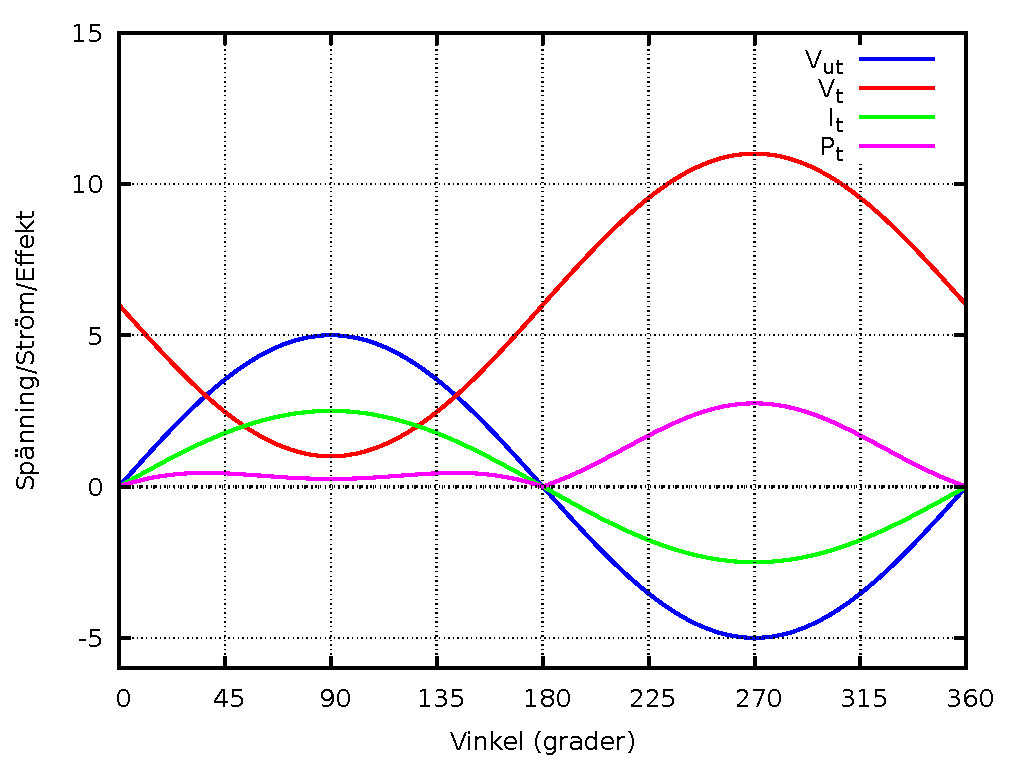
\includegraphics[width=7cm]{images/power1}
\caption{Utspänning $V_{ut}$, Transistor-spänning $V_t$, Transistor-ström $I_t$ och transistor-effekt $P_t$ varierar med vinkel sinus-signalen för resistiv last.}
\label{fig:power1}
\end{center}
\end{figure}

I bild \ref{fig:power1} ser vi utsignalen \(V_ut\) som en sinus med amplituden
\(5\ V\), dvs \(10\ V_{pp}\). Eftersom transistor har en vilo-spänning på 6~V
för att få marginal mot \(0\ V\) och \(+12\ V\), så kommer spänningen variera
mellan \(1\ V\) och \(11\ V\) och det ser man i \(V_t\) kurvan. Utgångslastens
resistor lastar med en ström \(I_t\) som är proportionerlig mot spänningen
\(V_{ut}\) på utgången. Effekten för transistorn \(P_t\) är sedan absolut-
funktionen för strömmen gånger spänningen, dvs. Joules lag. Den observante ser
att effekten är signifikant högre för andra halvan av kurvan, då man har både
hög spänning och hög ström.


%\part{REGLER OCH TRAFIKMETODER}

Naturlagarna begränsar frekvensområdet som kan användas för radiosändningar.
En del sändningar riktar sig till många lyssnare, andra sändningar sker
mellan två personer. Många radiosändningar delar på samma frekvensområde och
ingen part vill bli störd av någon annan.

För att minimera risken för störningar och utnyttja frekvensområdet effektivt
sker ett samarbete inom ITU mellan många länders administrationer och
radiotjänster.

Samarbetet tar fram hur frekvenserna och utrymmet för radiokommunikation ska
fördelas och användas samt prioriteringar om nyttjanderätt, sändningsslag,
effekter, räckvidder m.m.

Liksom det finns lagar och trafikbestämmelser för flyg, sjöfart och landtrafik
så regleras sedan mycket länge även radiotrafik av alla de slag. Utöver
nationella regler finns det mellanstatliga (bilaterala), regionala och
internationella överenskommelser om radiotrafik. Detta gäller även
amatörradiotrafik, som är en internationell radiotjänst.

Frekvensbanden för amatörradio har tilldelats vid internationella konferenser
där IARU har representerat radioamatörerna. De svenska föreskrifterna för
amatörradio påverkas därför av internationella intressen och överenskommelser.

Den \emph{internationella telekonventionen -- ITC --} är den
överenskommelse på vilken verksamheten inom den \emph{internationella
teleunionen -- ITU} -- bygger. Konventionen kompletteras av det internationella
Radioreglementet (ITU-RR), vilket omfattar huvudregler som överenskommits mellan
alla medlemmar inom ITU.

Konventionen och radioreglementet är bindande för alla stater som ratificerat
konventionen. De avsteg, som ett land vill göra och övriga länder godtar,
skrivs in som s.k. fotnoter. Radioreglementet omfattar alla radiotjänsters
verksamhet, däribland Amatör- och amatörsatellittjänsterna.

\textbf{OBSERVERA!  Som radioamatör är Du skyldig att följa gällande
  bestämmelser för amatörradioanvändning i det land som Du vistas i.
  Förvissa Dig om att Du har senaste utgåvan!  Vid osäkerhet --
  rådfråga PTS!}


%\section{Komponenter i serie och parallellt}

\subsection{Seriekopplade resistorer}
\textbf{HAREC a.\ref{HAREC.a.3.1.1a}\label{myHAREC.a.3.1.1a}}

Bild II 3-1

Den totala resistansen av seriekopplade resistorer är summan av resistanserna.

\[R = R_1 + R_2 + R_3 \cdots \]

Strömmen är lika stor genom alla seriekopplade resistorer i strömvägen (ingen
avgrening).

\[I = I_1 + I_2 + I_3 \cdots \]

Den totala spänningen över seriekopplade resistorer är summan av spänningen över
var och en av dem.

\[U = U_1 + U_2 + U_3 \cdots \]

Spänningen över var och en av seriekopplade resistorerförhåller sig som deras
resistanser. För två resistorer gäller

\[\frac{U_1}{U_2} = \frac{R_1}{R_2}\]


\subsection{Parallellkopplade resistorer}
\textbf{HAREC a.\ref{HAREC.a.3.1.1b}\label{myHAREC.a.3.1.1b}}

Bild II 3-2

Den totala resistansen av parallellkopplade resistorer är lägre än den lägsta
enstaka resistansen.

\[
\frac{1}{R} = \frac{1}{R_1} + \frac{1}{R_1} +
\frac{1}{R_2} + \frac{1}{R_3} + \cdots \frac{1}{R_n}
\]

För två resistorer gäller

\begin{align*}
\frac{1}{R} &= \frac{1}{R_1} + \frac{1}{R_2} && eller \\
R &= \frac{R_1 \cdot R_2}{R_1 + R_2}
\end{align*}

För tre resistorer gäller

\begin{align*}
\frac{1}{R} &= \frac{1}{R_1} + \frac{1}{R_2} + \frac{1}{R_3} && eller \\
R &= \frac{R_1\cdot R_2\cdot R_3}{R_1\cdot R_2 + R_1\cdot R_3 + R_2\cdot R_3}
\end{align*}

Strömmen förgrenar sig mellan parallellkopplade resistare r. Den totala strömmen
är summan av grenströmmarna

\begin{align*}
  I = I_1 + I_2 + \cdots I_n && \text{(Kirchhoffs 1:a lag)}
\end{align*}

Spänningen är lika stor över var och en av

\begin{align*}
  U = U_1 = U_2 = U_3 = \cdots U_n && \text{(Kirchhoffs 2:a lag)}
\end{align*}

Grenströmmarna genom parallellkopplade resistorer fördelar sig omvänt
proportionellt till deras respektive resistanser.
För två resistorer gäller

\[\frac{I_1}{I_2} = \frac{R_2}{R_1}\]

Bild II 3-1 Seriekopplade resistorer

Bild II 3-2 Parallellkopplade resistorer

\subsection{Spänningsdelare}

Bild II 3-3

Spänningsdelare förekommer i flera former. Bilden visar en spänningsdelare med
resistorer där spänningen \(U\) delas upp i spänningen \(U_1\) över resistorn
\(R_1\) respektive \(U_2\) över \(R_2\). Man kan då t.ex. använda spänningen för
något ändamål.

Ett alternativ till spänningsdelning med resistorer med fasta värden är
\emph{potentiometern}. Det är en variabel spänningsdelare i form av en resister
med ett uttag som kan flyttas mellan ändanslutningarna.

Om man nu ansluter en apparat parallellt över \(R_2\), t.ex. ett instrument
vars inre resistans motsvaras av \(R_y\), så kommer spänningarna över \(R_1\)
och \(R_2\) att påverkas.

Om \(R_y\) är mycket större än \(R_2\), så kan man bortse från påverkan.
För att beräkna \(U_2\) kan man då använda följande formel för en obelastad
resistiv spänningsdelare.

\begin{align*}
\frac{U_2}{R_2} &= \frac{U}{R_1 + R_2} \quad \text{eller} \\
U_2 &= U \cdot \frac{R_2}{R_1 + R_2}
\end{align*}

Om \(R_y\) däremot är av samma storleksordning eller lägre än \(R_2\), så måste
man för att beräkna \(U_2\) använda en formel för en belastad resistiv
spänningsdelare, t.ex.

\[
U_2 = U \cdot \frac{ \frac{R_2 \cdot R_y}{R_2 + R_y} }{ R_1 + \frac{R_2 \cdot R_y}{R_2 0 R_y} }
\]

Härav förstås att t.ex. en spänningsmätning ger olika resultat beroende på den
inre resistansen i voltmetern.

Bild II 3-3 Resistiv spänningsdelare

\subsection{Wheatstones brygga}

Bild II 3-4

En speciell tillämpning av spänningsdelare är en s.k. brygga (Wheatstones
brygga), som används för att jämföra spänningar.

Bryggan kan ses som två parallellkopplade spänningsdelare varav den ena är en
potentiometer med en skala graderad t.ex. i Ω. Den andra spänningsdelaren består
av en resister med känd resistans och en resisto r med okänd resistans, d.v.s.
mätobjektet.

I ledningen som förbinder de respektive mittuttagen X och Y, finns en
amperemeter som nollströmsindikator.


Det flyter ström mellan X och Y när det finns en potentialskillnad - spänning -
däremellan. Bryggan är då i obalans. Det flyter däremot ingen ström där när det
inte finns en potentialskillnad, d.v.s. när bryggan är i balans. Balans
(mätvärdet) får man genom justering av den graderade potentiometern till noll
ström. Då gäller sambandet

\[\frac{R_1}{R_2} = \frac{R_3}{R_4}\]

Bild 113-4 Wheatstones brygga

Spänningsdelare och bryggor har tagits med för att påvisa att apparater påverkar
varandra när de kopplas samman, vilket är fallet även vid mätningar.

Spänningsdelning kan även utföras med kondensatorer och induktorer förutsatt att
det är fråga om en växelströmskrets.

\subsection{Parallellkopplade kondensatorer}
\textbf{HAREC a.\ref{HAREC.a.3.1.1f}\label{myHAREC.a.3.1.1f}}

Bild II 3-5

I stället för en enda kondensator kan man parallellkoppla flera kondensatorer
för att uppnå önskad total kapacitans.

Den totala kapacitansen för parallellkopplade kondensatorer är summan av de
enskilda kapacitanserna.

\[C = C_1 + C_2 + C_3 + \cdots C_n\]

Räkneexempel:
\begin{enumerate}
\item \(C_1 = 5\ µF \quad C_2 = 10\ µF \quad C =\ ?\)
  \begin{align*}
    C &= C_1 + C_2 \\
    &= 5 + 10 \\
    &= 15\ µF
  \end{align*}
\item \(C_1 = 1\ nF \quad C_2 = 5\ pF \quad C =\ ?\)
  \begin{align*}
    C &= C_1 + C_2 \\
    &= 1 + 0.005 \\
    &= 1.005\ pF
  \end{align*}
\end{enumerate}

\subsection{Seriekopplade kondensatorer}
\textbf{HAREC a.\ref{HAREC.a.3.1.1e}\label{myHAREC.a.3.1.1e}}

Bild II 3-6

Den totala kapacitansen för seriekopplade kondensatorer är lägre än kapacitansen
för kondensatorn med det minsta värdet.

\[
\frac{1}{C} = \frac{1}{C_1} + \frac{1}{C_2} +
\frac{1}{C_3} + \cdots \frac{1}{C_n}
\]

För två kapacitanser gäller:

\begin{align*}
  \frac{1}{C} &= \frac{1}{C_1} + \frac{1}{C_2} \quad \text{eller} \\
  C &= \frac{C_1 \cdot C_2}{C_1 + C_2}
\end{align*}

För tre kapacitanser gäller:

\begin{align*}
  \frac{1}{C} &= \frac{1}{C_1} + \frac{1}{C_2} + \frac{1}{C_3}
  \quad \text{eller} \\
  C &= \frac{C_1 \cdot C_2 \cdot C_3}
  {C_1 \cdot C_2 + C_2 \cdot C_3 + C_2 \cdot C_3}
\end{align*}

Räkneexempel:

\[C_1 = 5\ µF \quad C_2 = 10\ µF \quad C =\ ?\]
\begin{align*}
  \frac{1}{C} &= \frac{1}{C_1} + \frac{1}{C_2} \\
  C &= \frac{C_1 \cdot C_2}{C_1 + C_2} \\
  &= \frac{5 \cdot 10}{5 + 10}\ µF \\
  &= 3\frac{1}{3}\ µF \\
  &\approx 3.33\ µF
\end{align*}

Bild II 3-5 Parallellkopplade kondensatare

Bild II 3-6 Seriekopplade kondensatorer

\subsection{Galvaniskt kopplade induktorer}

Induktansvärdet för galvaniskt sammankopplade induktorer kan i princip
beräknas på samma sätt som för motsvarande sammankoppling av resistorer.

\subsubsection{Galvaniskt seriekopplade induktorer}
\textbf{HAREC a.\ref{HAREC.a.3.1.1c}\label{myHAREC.a.3.1.1c}}

Förutsatt att magnetfälten från de respektive induktorerna inte återverkar på
varandra - d.v.s. inte ``kopplar magnetiskt till varandra'' - så gäller:

\[L = L_1 + L_2 + L_3 + \cdots L_n\]

Räkneexempel:

\[L_1 = 20\ mH \quad L_2 = 50\ mH \quad L =\ ?\]
\begin{align*}
  L &= L_1 + L_2 \\
  & = 20 + 50 \\
  &= 70\ mH
\end{align*}

\subsubsection{Galvaniskt parallellkopplade induktorer}
\textbf{HAREC a.\ref{HAREC.a.3.1.1d}\label{myHAREC.a.3.1.1d}}

Förutsatt att magnetfälten från de respektive induktorerna inte återverkar på
varandra - d.v.s. inte ``kopplar magnetiskt till varandra'' - så gäller:

\[
\frac{1}{L} = \frac{1}{L_1} + \frac{1}{L_2} + \frac{1}{L_3} +
\cdots \frac{1}{L_n}
\]

För två induktorer gäller:

\begin{align*}
  \frac{1}{L} &= \frac{1}{L_1} + \frac{1}{L_2} \quad \text{eller} \\
  L &= \frac{L_1 \cdot L_2}{L_1 + L_2}
\end{align*}

Räkneexempel:

\[L_1 = 50\ mH \quad L_2 = 60\ mH \quad L =\ ?\]
\begin{align*}
  L &= \frac{L_1 \cdot L_2}{L_1 + L_2} \\
  &= \frac{50 \cdot 60}{50 + 60}\ mH \\
  &= \frac{3000}{110}\ mH \\
  &\approx 27\ mH
\end{align*}

\subsection{Magnetiskt kopplade induktorer}

I praktiken anordnas ofta induktorer så, att deras respektive magnetfält kan
återverka på varandra - s.k. magnetisk koppling.

En \emph{ömsesidig induktans} \(M\) uppstår i induktorerna på grund av denna
koppling. Den ömsesidiga induktansen ökar eller minskar det resulterande
induktansvärdet beroende på om induktorernas magnetfältverkar med eller mot
varandra.

Beräkningen av värdet på \(M\) är emellertid relativt komplicerad och behandlas
ej här. I stället görs en förenklad framställning.

Bild II 3-7 Magnetiskt kopplade induktorer

Bild II 3-7

Bilden visar seriekopplade induktorer, vars magnetfält kopplar till varandra på
olika sätt. ``Pricken'' vid änden av induktorerna på bilden markerar att
magnetfälten där har inbördes polarisering.

\emph{Magnetiskt kopplade induktorer i serie}

Formel:

\[L = L_1 +L_2 \pm 2M\]

Räkneexempel:

Två induktorer har en impedans av 20 resp. 1O µH och en ömsesidig induktans av
2 µH. Induktorerna är kopplade och placerade så att deras magnetfält verkar med
varandra.

Vardera induktansen ökas därför med \(M = 2\ µH\).

\begin{align*}
  L &= L_1 + M + L_2 + M \\
  &= 20 + 2 + 10 + 2\ µH \\
  &= 34\ µH
\end{align*}

Räkneexempel:
Två induktorer har en impedans av 20 resp 1O µH och en ömsesidig induktans av
2µH. Induktorerna är kopplade och placerade så att deras magnetfält verkar mot
varandra. Vardera induktansen minskas därför med \(M = 2\ µH\).

\begin{align*}
  L &= L_1 - M + L_2 - M \\
  & = 20 - 2 + 10 - 2\ µH \\
  &= 28\ µH
\end{align*}

\emph{Magnetiskt kopplade induktorer i parallell}

Formel:

\[L = \frac{L_1 \cdot L_2 \cdot M^2}{L_1 + L_2 + M^2}\]

\subsection{Upp- och urladdning av en kondensator}

\subsubsection{Uppladdning}

Bild II 3-8

En kondensator \(C\) seriekopplas med en resistans \(R\)
och kopplas in över spänningen \(U\).

Spänningen över kondensatorn stiger från 0 volt till \(U_{max}\).

Laddningsströmmen sjunker från \(I_{max}\) till 0 ampere.

Spänningen över kondensatorn ökar exponentiellt uppladdningen.

\[u_c = U_{max} \cdot ( 1 - e^{-\frac{t}{\tau}} )\]

\begin{tabular}{lp{6cm}}
  \(u_c\)     & spänningen över kondensatorn efter en given inkopplingstid \\
  \(U_{max}\) & slutspänningen efter minst \(t = 5\tau\) \\
  \(t\)       & inkopplingstiden \\
  \(e\)       & 2.718 (e = basen för den naturliga logaritmen) \\
\end{tabular}

I förloppet ingår storleken av resistans och kapacitans enligt följande samband,
som kallas tidskonstant:

\[\tau = R \cdot C\]

\[C\ [\text{F}] \quad R\ [Ω] \quad s [\text{sek}] \quad \tau [\text{tidskonstant i sek}]\]

Efter tiden \(t = 1\tau\) från inkopplingsögonblicket har spänningen över
kondensatorn ökat från noll till 63\% av maxvärdet. Efter tiden \(t = 5\tau\)
är kondensatorn uppladdad till 99\%.

\emph{Strömmen} från kondensatorn minskar exponentiellt under uppladdningen.

\[i_c = I_{max} \cdot e^{-\frac{t}{\tau}}\]

\begin{tabular}{lp{6cm}}
  \(i_c\) & strömmen från kondensatorn efter en given inkopplingstid \\
  \(I_{max}\) & begynnelseströmmen \\
\end{tabular}

Efter tiden \(t = 1\tau\) från inkopplingsögonblicket har strömmen till
kondensatorn minskat till 37\% av maxvärdet.

Efter tiden \(t = 5\tau\) återstår 1\% av strömmens maxvärde.

Bild II 3-8 Uppladdning av en kondensator

\subsubsection{Urladdning}

Bild II 3-9

En kondensator C urladdas över resistor R.

\emph{Spänningen} över kondensatorn minskar exponentiellt under urladdningen.

\[u_c = U_{max} \cdot e^{-\frac{t}{\tau}}\]

\emph{Strömmen} från kondensatorn minskar exponentiellt under urladdningen.
Strömriktningen är motsatt den vid uppladdningen.

\[i_c = - I_{max} \cdot e^{-\frac{t}{\tau}}\]

Efter tiden \(t = 1\tau\) är kondensatorn urladdad så, att 37\% av \(I_{max}\)
respektive \(U_{max}\) återstår.

Efter tiden \(t = 5\tau\) är kondensatorn urladdad så, att mindre än 1\% av
\(I_{max}\) respektive \(U_{max}\) återstår.

Exempel på beräkning av tidskonstanten:
\begin{enumerate}
\item \(C = 10\ µF \quad R = 1 kΩ \quad \tau =\ ?\)
  \begin{align*}
    \tau &= R \cdot C \\
    &= 1 \cdot 10^3 \cdot 10 \cdot 10^{-6} \\
    &= 10 \cdot 10^{-3} \quad \text{dvs var 1/100 sekund.}
  \end{align*}
\item \(C = 10000\ µF \quad R = 1 kΩ \quad \tau =\ ?\)
  \begin{align*}
    \tau = R \cdot C \\
    &= 1 \cdot 10^3 \cdot 10^3 \cdot 10^{-6} \\
    &= 1\ \text{sekund}
  \end{align*}
\end{enumerate}

Bild II 3-9 Urladdning av en kondensator

\subsection{In- och urkoppling av en induktor}

\emph{Inkoppling}

Bild II 3-10

En induktor L i serie med en resistans R kopplas in över en likspänning U.
Spänningen över induktorn ökar från 0 till \(U_{max}\).

(Egentligen, induktorns motspänning minskar så att...)

Strömmen genom induktorn ökar från 0 till \(U_{max}\).

Strömmen genom induktorn ökar exponentiellt efter inkopplingen

\[i_L = I_{max} \cdot (1-e^{-\frac{t}{\tau}} )\]

\begin{tabular}{lp{5cm}}
  \(i_L\) &  strömmen efter en given inkopplingstid \\
  \(I_{max}\) & slutströmmen efter minst \(t = 5\tau\) \\
  \(t\) & inkopplingstiden \\
  \(e\) & 2.718 (e = basen för den naturliga logaritmen) \\
\end{tabular}

I förloppet ingår storleken av resistans och induktans enligt följande samband,
som kallas tidskonstant

\[\tau = \frac{L}{R}\]

\[
L\ [\text{H}] \quad
R\ [Ω] \quad
s\ [\text{sek}] \quad
\tau\ [\text{tidskonstant}]
\]

Efter en tid av \(t = 1\tau\) från inkopplingsögonblicket har strömmen genom
induktorn ökat från noll till 63\% av \(I_{max}\) och motspänningen över
induktorn minskat till 37\% av maxvärdet.

\emph{Urkoppling}

Spänningskällan kopplas bort från samma induktor som ovan. En resister är
inkopplad över induktorn. Energin i induktorn avleds genom resistorn som en
ström med motsatt riktning än vid inkopplingen. Strömmen är vid
urkopplingstillfället \(I_{max} = i_L\) och minskar därefter exponentiellt.

\[i_L = I_{max} \cdot e^{-\frac{t}{\tau}}\]

\begin{tabular}{lp{5cm}}
  \(i_L\) & strömmen genom induktorn efter en given urkopplingstid \\
  \(I_{max}\) & strömmen i urkopplingsögonblicket \\
  \(e\) & 2.718 \\
  \(t\) & tiden efter urkopplingsögonblicket \\
\end{tabular}

Efter en tid av \(t = 1\tau\) från urkopplingsögonblicket har strömmen genom
induktorn minskat till 37\% av maxvärdet.

Teoretiskt kan spänningarna och strömmarna aldrig nå ett noll- eller maxvärde,
men för praktiskt bruk anses detta inträffa efter en tid av minst \(5\tau\).

All den energi som lagras i en induktor finns i dess magnetfält. När strömmen
bryts eller minskas så återgår energin omedelbart till kretsen. I en induktor
kan det således inte finnas någon kvarstående energi, vilket det däremot kan
göra i en kondensator.

Under den tid som magnetfältet i en induktor avvecklas eller byggs upp, så
induceras en motspänning i den. Denna spänning är högre än den som finns över
induktorn innan strömmen bryts eller ändras och är proportionell till den
hastighet som ändringen har. När en en strömkrets med induktor
bryts är det vanligt att det i brytögonblicket bildas en gnista eller ljusbåge
över brytarens kontakter.

Om induktansen är stor och kretsströmmen hög, så skall en stor mängd energi
frigöras på mycket kort tid. Det är därför inte ovanligt att brytarkontakter
bränns eller smälter. I likströmskretsar kan gnistan eller ljusbågen minskas
eller undertryckas genom att en kondensator i serie med en resistor kopplas
över kontaktstället. Kondensatorn fångar upp en del av energin i induktorn och
resistorn minskar hastighetsändringen.

Bild II 3-10 Inkoppling av en induktor

\subsection{Växelströmskretsar}

\subsubsection{Komponentegenskaper vid växelström}

Inom radiotekniken används mycket ofta svängningskretsar bestående av
kondensatorer och induktorer, som är kopplade i serie eller parallellt med
varandra. När svängningskretsens egenfrekvens sätts lika med frekvensen på den
signal som tillförs kretsen, så får kretsen särskilda egenskaper som används på
olika sätt.

För att förstå hur ``LC-kretsar'' fungerar, beskrivs först hur de ingående
komponenternas resistans, induktans och kapacitans förhåller sig till varandra,
när de kombineras och kopplas til en växelströmkälla.

Bild II 3-11

Bilden visar amplituden av spänning och ström vid ett sinusformat förlopp samt
den effekt som då utvecklas. Tidsaxeln är graderad O - 360° per period.

\emph{Fall a:} Förloppen med en resister R.

Med en resister följer ström- och spänningskurvorna varandra tidsmässigt, även
vid riktningsändring. När kurvorna följs åt på det sättet, sägs de vara i fas
med varandra.

Effekt överförs från strömkällan till resistorn. Den effekt som utvecklas i
resistorn är, vid varje tidpunkt av perioden, produkten av strömmmen och
spänningen just då. Eftersom storheterna av spänning och ström är antingen
positiva eller negativa samtidigt, så blir produkten alltid positiv. Det betyder
att den effekt som utvecklas pulserar två gånger per period mellan ett noll- och
maxvärde.

\emph{Fall b:} Förloppen med en induktor L.

Med en induktor är utvecklingen av ström och spänning inte samtidig. Vid
inkopplingen stiger spänningen genast till maxvärdet medan strömmen stiger
långsammare och bygger under tiden upp ett magnetfält i induktorn och omkring
övriga ledare i kretsen.

Bild II 3-11 Faslägen och effekter i L C-kretsar

Strömmen fördröjs alltså i förhållande till spänningen. Eftersom kurvornas max-
och nollvärden inträffar vid olika tidpunkter, så heter det att de är
\emph{ur fas} eller \emph{fasförskjutna}.

En växelström genom en ideal induktor ärtasförskjuten 90° \emph{efter}
spänningen. Strömmen når toppvärdet vid tidpunkten 90° av perioden, när
spänningen nått ner till noll. När spänningen minskar, så sjunker strömmen och
tar med sig energin i magnetfältet. Först vid 180°, när spänningen har nått
maxvärdet åt andra hållet, ändrar också strömmen riktning och bygger upp ett
nytt magnetfält med motsatt polaritet.

Effekt överförs från strömkällan till induktorn när ström och spänning har samma
riktning. När ström och spänning har olika riktning, försöker induktorn i
stället ``ladda'' strömkällan med energi från sitt kraftfält. Det pendlar därför
effekt mellan strömkällan och induktorn, varvid effekten i ena riktningen är
lika stor som i andra riktningen.

Sett över en hel period upphäver därför dessa effekter varandra. Följden blir
att en ideal induktor, i motsats till en resistor, inte förbrukar någon aktiv
effekt. Man säger att en reaktans, här en induktor, arbetar med reaktiv effekt.

I praktiken har kretsen även en viss resistans. Därför sätts reaktansens 90°
fasörskjutna ström samman med resistansens 0° fasförskjutna ström. Resultatet
blir en ström, som är mindre än 90° ur fas, och det förbrukas då en viss aktiv
effekt i resistansen.


\emph{Fall c:} Förloppen med en kondensator C.

Inte heller med en kondensator utvecklas ström och spänning samtidigt. Efter
inkopplingen laddar strömmen upp kondensatorn, d.v.s. bygger upp ett elektriskt
fält med en viss potential (spänning). Spänningen utvecklas långsammare än
strömmen - den blir \emph{fasförskjuten}.

Strömmen till (och från) en ideal kondensator är fasförskjuten 90° före
spänningen. När kondensatorn är kopplad till en växelströmskälla, når strömmen
toppvärdet vid tidpunkten 90° eller 270° av perioden. Spänningen passerar då i
båda fallen värdet noll. När spänningen minskar, så sjunker strömmen och tar
energi ur det elektriska fältet.

Sedan strömmen passerat noll vid 180° eller 0°/360°, bygger den upp ett nytt
magnetfält med motsatt polaritet.

$>>>>>$ TODO: Här ska det väl stå elektriskt fält?

Liksom med en induktor överförs effekt från strömkällan till kondensatorn när
ström och spänning har samma riktning. När ström och spänning har olika
riktning, försöker kondensatorn i stället "ladda" strömkällan med energi. Det
pendlar därför effekt mellan strömkällan och kondensatorn, varvid effekten i
ena riktningen är lika stor som i andra riktningen.

Sett över en hel period upphäver därför dessa effekter varandra. Följden blir
att en ideal kondensator, i motsats till en resistor, inte förbrukar någon
aktiv effekt. Man säger då, att en reaktans, här en kondensator, arbetar med
\emph{reaktiv} effekt.

I praktiken har kretsen även en viss resistans. Därför sätts reaktansens 90°
fasförskjutna spänning samman med resistansens 0° fasförskjutna ström.
Resultatet blir en spänning, som är mindre än 90° ur fas, och det förbrukas då
en viss aktiv effekt i resistansen. Som framgår av bilden blir variationerna i
tiden de omvända med kondensator jämfört med induktor.

\subsection{Impedans}
\textbf{HAREC a.\ref{HAREC.a.3.2.2}\label{myHAREC.a.3.2.2}}

Liten ordlista:
\begin{itemize}
\item Impedans - hindra (lat. impedire).
\item Resistans - motstå (lat. resistere).
  Del av impedansen, kallas ibland ohmskt motstånd.
\item Reaktans- återverka (lat. reagere).
  Del av impedansen, samlingsord för växelströmsmotstånd.
  \begin{itemize}
  \item Kapacitans- inrymma (lat. capax). Del av reaktansen.
  \item Induktans - införa (lat. inducere). Del av reaktansen.
  \end{itemize}
\end{itemize}

Hittills har storheterna resistans, induktans och kapacitans behandlats var för
sig, men i praktiken förekommer de alltid tillsammans och kallas impedans.

Resistansen är i princip oförändrad vid ström- eller spänningsändringar. Men när
strömmen genom en ledare eller induktor liksom spänningen över en kondensator
ändras, så tillkommer en reaktans som motverkar förändringarna.

Reaktansen kan från fall till fall vara kapacitiv eller induktiv och ingår i
impedansen. Om ingen reaktans finns, så är impedansen lika med resistansen.

Bild II 3-12

Bilden visar en induktor, en kondensator och en resistor som är kopplade i
serie. När man vill beräkna den resulterande impedansen i kretsen
(``totala växelströmsmotståndet''), måste man ta hänsyn till att komponenternas
spänningar eller strömmar inte är i fas med varandra. De arbetar ju inte
``i takt''.

Att då addera max. värdena ger fel resultat. I stället söker man den s.k.
resultanten av de olika vektorer som motsvarar strömoch spänningsvärden.
Detta kan göras grafiskt eller beräknas.

Bild 113-13

Vi tänker oss att vektorerna i systemet vrider sig moturs med hastigheten
\(\omega = 2πf\) där \(f\) är frekvensen och \(\omega\) är vinkelhastighet.
Eftersom vektorerna har samma frekvens, så är vektorernas lägen inbördes samma.
Ögonblicksvärdet av respektive vektorer följer en sinuskurva.

Spänningsvektorn i den ``induktiva reaktansen'' ligger 90° före strömmen och
spänningen i resistansen. Spänningsvektorn i den ``kapacitiva reaktansen''
ligger 90° efter strömmen och spänningen i resistansen. Vektorerna i dessa två
reaktanser är således \(2 \cdot 90 = 180°\) åtskilda, d.v.s. motriktade.
Det kallas att de är i motfas.

Bild II 3-14

l bilden visas vektorerna för komponenterna i Bild II 3-12 samt hur man grafiskt
bestämmer inpedansen av dessa vektorer. Vidare får man fasvinkeln mellan
impedansens och resistansens vektor, varav den senare är den s.k. riktfasen för
hela seriekretsen.

Bild II 3-12 Seriekrets av L+C+R

Bild II 3-13 Spänningar i seriekrets L+C+R

Bild II 3-14 Impedansen och fasvinkeln i seriekrets L+C+R

Resistansen ritas som en vektor R, som riktas vågrätt mot höger. Vektorns längd
motsvarar resistansens storhet i ohm.

Den induktivareaktansen ritas på liknande sätt med vektorn \(X_L\) lodrätt
uppåt. Slutligen ritas den kapacitiva reaktansen Xc lodrätt neråt.

Man subtraherar de motverkande reaktiva vektorerna \(X_L\) och \(X_c\) från
varandra och avsätter resultatet \(X\) på den vertikala axeln, uppåt om \(X_L\)
är större och neråt om \(X_c\) är större. Den resistiva vektorn R avsätts åt
höger på den horisontella axeln.

Man låter nu vektorerna X och R bilda sidor i en rätvinklig rektangel. Längden
på rektangelns diagonal är den resulterande impedansen Z. Fasvinkeln mellan
impedans och resistans kan också avläsas.

Eftersom vektordiagrammet bildar en rätvinklig triangel kan den resulterande
spänningen U i kretsen även beräknas med Pytagoras sats:

\[C^2 = A^2 + B^2 \quad eller \quad C = \sqrt{A^2 + B^2}\]

Tillämpad på ovanstående vektordiagram kan satsen skrivas som

\[U_{LCR}^2 = U_R^2 + ( U_L - U_C)^2\]

Termerna ersätts med följande ekvationer:

\begin{align*}
  U_{LRC} &= I \cdot Z \\
  U_R &= I \cdot R \\
  U_L &= I X_L = I \omega L \\
  U_C &= I X_C = I \frac{1}{\omega C} \\
  I^2 Z^2 &= I^2 R^2 + ( I \omega L - I\frac{1}{\omega C})^2
\end{align*}

Efter division med \(I^2\) fås

\begin{align*}
  Z^2 &= R^2 + ( \omega L - \frac{1}{\omega L} )^2 \quad \text{eller} \\
  Z &= \sqrt{R^2 + (\omega L - \frac{1}{\omega L})} \quad \text{eller} \\
  Z &= \sqrt{R^2 + (X_L - X_C)^2}
\end{align*}

I en seriekrets är den resulterande reaktansen negativ (kapacitiv) om \(X_c\) är
större än \(X_L\) och positiv (induktiv) om \(X_L\) är större än \(X_C\).

\subsection{Ohms lag vid växelström}

I formler betecknas impedansen med bokstaven \(Z\) och reaktansen med bokstaven
\(X\). I båda fallen är sorten Ohm [\(Ω\)].

Vid beräkning av impedans är Ohms lag inte direkt tillämplig, eftersom
reaktansen i en induktor eller kondensator uppträder annorlunda i tiden vid
ström- respektive spänningsändring än vad resistansen gör.

Om impedansen \(Z\) sätts in i Ohms lag, så fås följande samband som ofta kallas
Ohms lag för växelström, således

\begin{align*}
  U_{eff} &= I_{eff} \cdot Z \quad \text{eller} \\
  U_{eff} &= I_{eff} \cdot \sqrt{R^2 + X^2} \quad \text{eller} \\
  U_{eff} &= I_{eff} \cdot \sqrt{R^2 + (X_L - X_C)^2} \quad \text{o.s.v.}
\end{align*}

Av vad som framgått tidigare i detta avsnitt kan även slutsatsen dras att:

\[
\text{skenbar effekt} = \sqrt{(\text{aktiv effekt})^2 + (\text{(reaktiv effekt})^2}
\]

\subsection{LC-kretsar}
\textbf{HAREC a.\ref{HAREC.a.3.2.1}\label{myHAREC.a.3.2.1}}

\subsubsection{Parallellkopplade LC-kretsar}

Bild II 3-15

En parallellkopplad LC-krets är ansluten till växelspänningen \(U\) från en
signalgenerator med inställbar frekvens \(f\). Två fall studeras.

Fall 1 : \(f = f_{res}\)

Signalgeneratorns frekvens \(f\) ställs lika med LC-kretsens resonansfrekvens
\(f_{res}\). Då visar kretsen hög impedans \(Z\) mot generatorn. En stark ström
cirkulerar i svängningskretsen, men endast en svag ström flyter i ledningen
mellan generator och krets. Jämför med modellförsöket på bild II 3-17.

Fall 2: \(f > f_{res}\) eller \(f < f_{res}\)

Frekvensen \(f\) ställs högre eller lägre än kretsens resonansfrekvens
\(f_{res}\).

Svängningskretsen visar då en låg impedans \(Z\) mot generatorn. En svag ström
cirkulerar i svängningskretsen, medan en starkare ström flyter i ledningen
mellan generator och krets.

I praktiken finns även en resistans (belastning) parallellt över kretsen och en
resistans i serie med induktansen. För enkelhetens skull bortses här från dessa
resistanser.

I en parallellkopplad LC-krets är spänningen över induktans och kapacitans
densamma. Spänningsvektorn \(U\) används därför som s.k. riktfas.

Riktfasen riktas på bilden åt höger. Strömmen \(I_C\) genom kondensatorn är
fasförskjuten 90° efter \(U\) och ritas rakt neråt (vektorerna roterar motsols).
Strömmen \(I_L\) genom induktorn är fasförskjuten 90° före \(U\) och ritas rakt
uppåt. Den resulterande reaktiva strömmen genom kretsen är skillnaden mellan
strömmarna \(I_C\) och \(I_L\), vilka är motriktade varandra.

Formeln för parallellkopplade resistanser kan även användas för
parallellkopplade reaktanser om man tillämpar Pytagoras sats
\(A^2 + B^2 = C^2\), således

\begin{gather*}
  \frac{1}{R} = \frac{1}{R_1} + \frac{1}{R_1} + \cdots \\
  \left(\frac{1}{Z}\right)^2 = \left(\frac{1}{R}\right)^2 +
  \left(\frac{1}{R}\right)^2 \quad \text{eller}
\end{gather*}
\begin{align*}
  \frac{1}{Z} &=
  \sqrt{\left(\frac{1}{R}\right)^2 + \left(\frac{1}{X}\right)^2} \\
  &= \sqrt{\frac{1}{R^2} + \frac{1}{X^2}}
\end{align*}

Med R försumbart kan den resulterande reaktansen av kapacitansen \(X_C\) och den
vektormässigt motriktade induktansen \(X_L\) beräknas på följande sätt:

\begin{align*}
  \frac{1}{X} &= \frac{1}{X_C} - \frac{1}{X_L} \quad \text{d.v.s.} \quad
  \frac{1}{X} = \frac{X_L - X_C}{-X_L \cdot X_C} \quad \text{eller} \\
  X &= \frac{-X_L \cdot X_C}{X_L - X_C}
\end{align*}

I en parallellkopplad LC-krets är den resulterande reaktansen negativ
(kapacitiv) om \(X_L\) är större än \(X_C\) och positiv (induktiv) om \(X_L\) är
mindre än \(X_C\).

Bild II 3-15 Parallellkopplad LC-krets

\subsection{Seriekopplade LO-kretsar}

$>>>>>$ TODO: Ersätt bilden med bilden från erratan.

Bild II 3-16

Bild II 3-16 Seriekopplad LC-krets

En seriekopplad LC-krets ansluts till växelspänningen U från en signalgenerator
med inställbar frekvens \(f\). Två fall studeras.

Fall 1: \(f = f_{res}\)

Signalgeneratorns frekvens \(f\) ställs lika med svängningskretsens
resonansfrekvens \(f_{res}\). Impedansen \(Z\) i en seriekrets visar då ett
mycket lågt värde mot generatorn. Det flyter en stark ström i ledningen mellan
generator och krets.

Fall 2: \(f < f_{res} \quad \text{eller} \quad f > f_{res}\)

Frekvensen \(f\) ställs lägre eller högre än kretsens resonansfrekvens
\(f_{res}\).

Eftersom svängningskretsen då visar hög impedans \(Z\) mot generatorn, så
flyter endast en svag ström i ledningen mellan generator och krets.

I praktiken finns även en resistans i serie med induktansen liksom en
parallellt över kapacitansen. För enkelhetens skull bortses här från dessa
resistanser.

Strömmen I är samma genom hela kretsen och strömvektorn I används därför som
s.k. riktfas. Den ritas i bilden åt höger. Om serieresistansen R varit med, så
skulle ett spänningsfall \(U_R\) varit inritad i samma riktning som I
(i fas med I). Spänningen över reaktansen \(X_C\) ligger 90° efter I och ritad
rakt neråt (vektorerna roterar motsols). Spänningen över reaktansen \(X_L\)
(induktorn) ligger 90° före I och ritad rakt uppåt.

\subsection{Thomsons svängningskrets}
\textbf{HAREC a.\ref{HAREC.a.3.2.4}\label{myHAREC.a.3.2.4}}

Bild II 3-17

Bild II 3-17 Thomsons svängningskrets

Bilden visar en svängningskrets, som består av en kondensator och en induktor
med förskjutbar järnkärna. En ändring av kärnans tvärsnitt ändrar den
magnetiska ledningsförmågan och därmed induktansen.

Med anordningen kan resonansfrekvensen alltså ställas in så att den blir högre,
lika med eller lägre än den anslutnaspänningens frekvens. Tre fall undersöks:
\begin{enumerate}
\item \(X_L > X_c\) LA1 och LA2 lyser upp, en kraftig ström flyter genom
  kondensatorn,
\item \(X_L < X_C\) LA1 och LA3 lyser upp, en kraftig ström flyter genom
  induktorn,
\item \(X_L= X_C\) LA2 och LA3 lyser upp, LA1 lyser inte, en kraftig ström
  flyter i kretsen men inte i tilledningarna
\item \(X_L = X_C\) kallas Thomson's svängningsformel, vilken beskriver
  resonansfallet
\end{enumerate}

Då är de induktiva och kapacitiva reaktanserna i kretsen lika stora och tar ut
varandra. Kvar är kretsens resistans, vilken vi tills vidare betraktar som
försumbar.
Således \(X_L = X_C\), där

\[X_L = 2πfL \quad \text{och} \quad X_C = \frac{1}{2πfC} \quad \text{sätts in.}\]
\begin{align*}
  2πfL = \frac{1}{2πfC} & \quad & 4π^2f^2LC = 1 \\
  f^2 = \frac{1}{4π^2LC} & \quad & f = \frac{1}{2π\sqrt{LC}}
\end{align*}
\[f\text{ [Hz] }L\text{ [H] }C\text{ [F] }\]

Formeln gäller både för parallell- och seriekretsar.

Räkneexempel:

\[L = 100\ nH \quad C = 10\ pF \quad f =\ ?\]
\begin{align*}
  f &= \frac{1}{2π\sqrt{100 \cdot 10^{-9} \cdot 10 \cdot 10^{-12}}} \\
  &= \frac{1}{2π10^{-1}} \\
  &= \frac{10^9}{2π} \\
  &\approx 159\ MHz
\end{align*}

\subsection{Impedansen i en resonant krets}
\textbf{HAREC a.\ref{HAREC.a.3.2.3}\label{myHAREC.a.3.2.3}}

En enkel framställning görs av hur impedans, reaktans och resistans förhåller
sig inbördes när en svängningskrets är i resonans. Som exempel används följande
kretsdata: Induktans 200 J.lH, kapacitans 200 p F, förlustresistans 1O Ω.

\subsubsection{Resonansfallet i en parallellkrets}
\label{parallellresonans}
\index{parallellresonans}
\index{resonans!parallellkrets}

Parallellkretsen består i sig själv av seriekopplade komponenter, varav
\(X_L\) och \(X_C\) är reaktiva. Vid resonans är dessa lika stora och
motverkande. Inom kretsen är således den resulterande reaktansen:

\[X_L - X_C = 0\]

Därför uppvisar samma krets en yttre reaktans av:

\[
  X = \frac{-X_L \cdot X_C}{X_L - X_C}
  = \frac{-X_L \cdot X_C}{0}
  = \infty
\]

I praktiken finns i kretsen också en resistans varför dessa extremvärden inte
uppstår. Inne i en parallellkrets i resonans cirkulerar alltså en stark ström,
som endast begränsas av kretsens resistans.

\begin{figure}[h]
\begin{center}
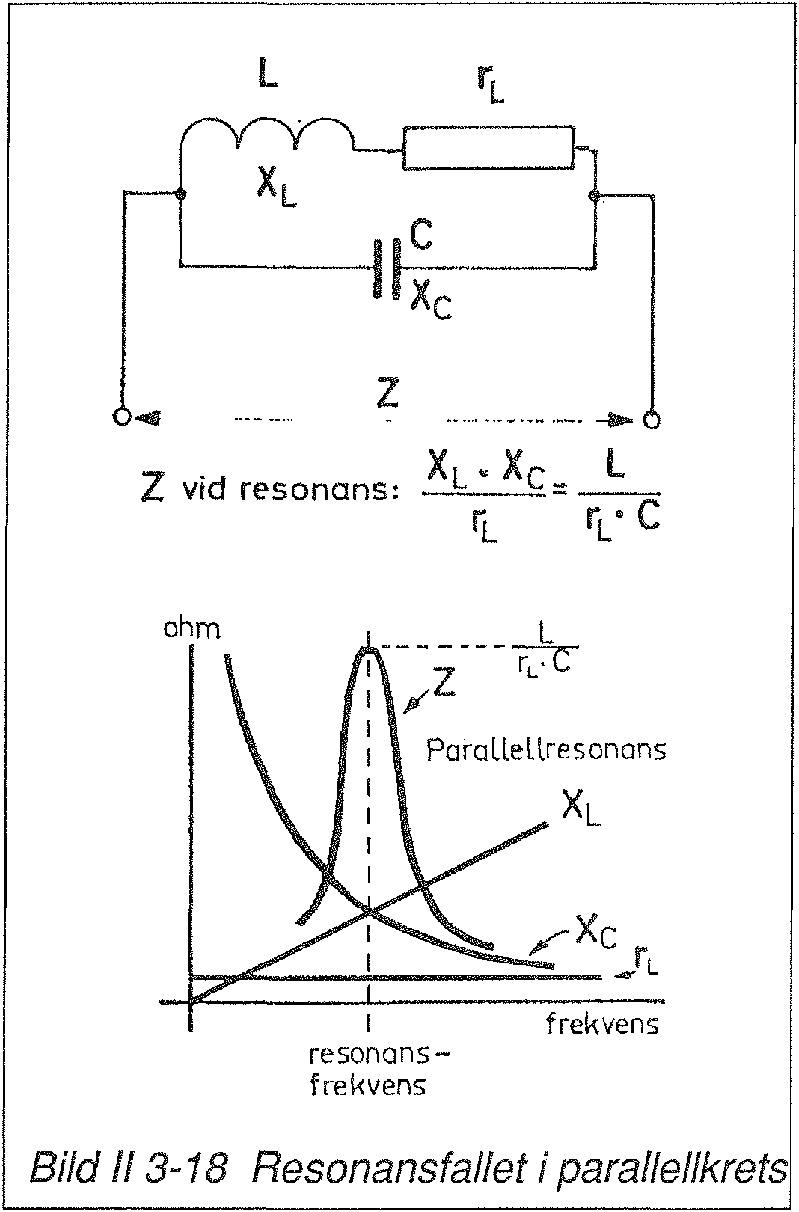
\includegraphics[width=7cm]{images/bild_2_3-18}
\caption{Resonansfallet i parallellkrets}
\label{fig:BildII3-18}
\end{center}
\end{figure}

Bild \ref{fig:BildII3-18}

Bilden visar en parallellkrets där induktorn har resistansen \(r_L\) och
kondensatorn antas vara förlustfri. Vidare förutsätts att kretsen är i resonans.

Vid resonans kan termen \(X_L - X_C = 0\) bytas mot \(r_L\) i formeln
\[X = \frac{-X_L \cdot X_C}{X_L - X_C}\] förutsatt att \(r_L\) är försumbart
jämfört med \(X_L\).

Därtill är \(X_L = 2πfL\) och \(X_C = \frac{1}{2πfC}\) d.v.s.
\(X_L \cdot X_C = \frac{L}{C}\) som sätts in.

Parallellkretsens impedans vid resonans kan då skrivas

\[
Z = \frac{X_L \cdot X_C}{r_L} = \frac{L}{r_L \cdot C}
\]

\subsubsection{Resonansfallet i en seriekrets}
\label{serieresonans}
\index{serieresonans}
\index{resonans!seriekrets}

\begin{figure}[h]
\begin{center}
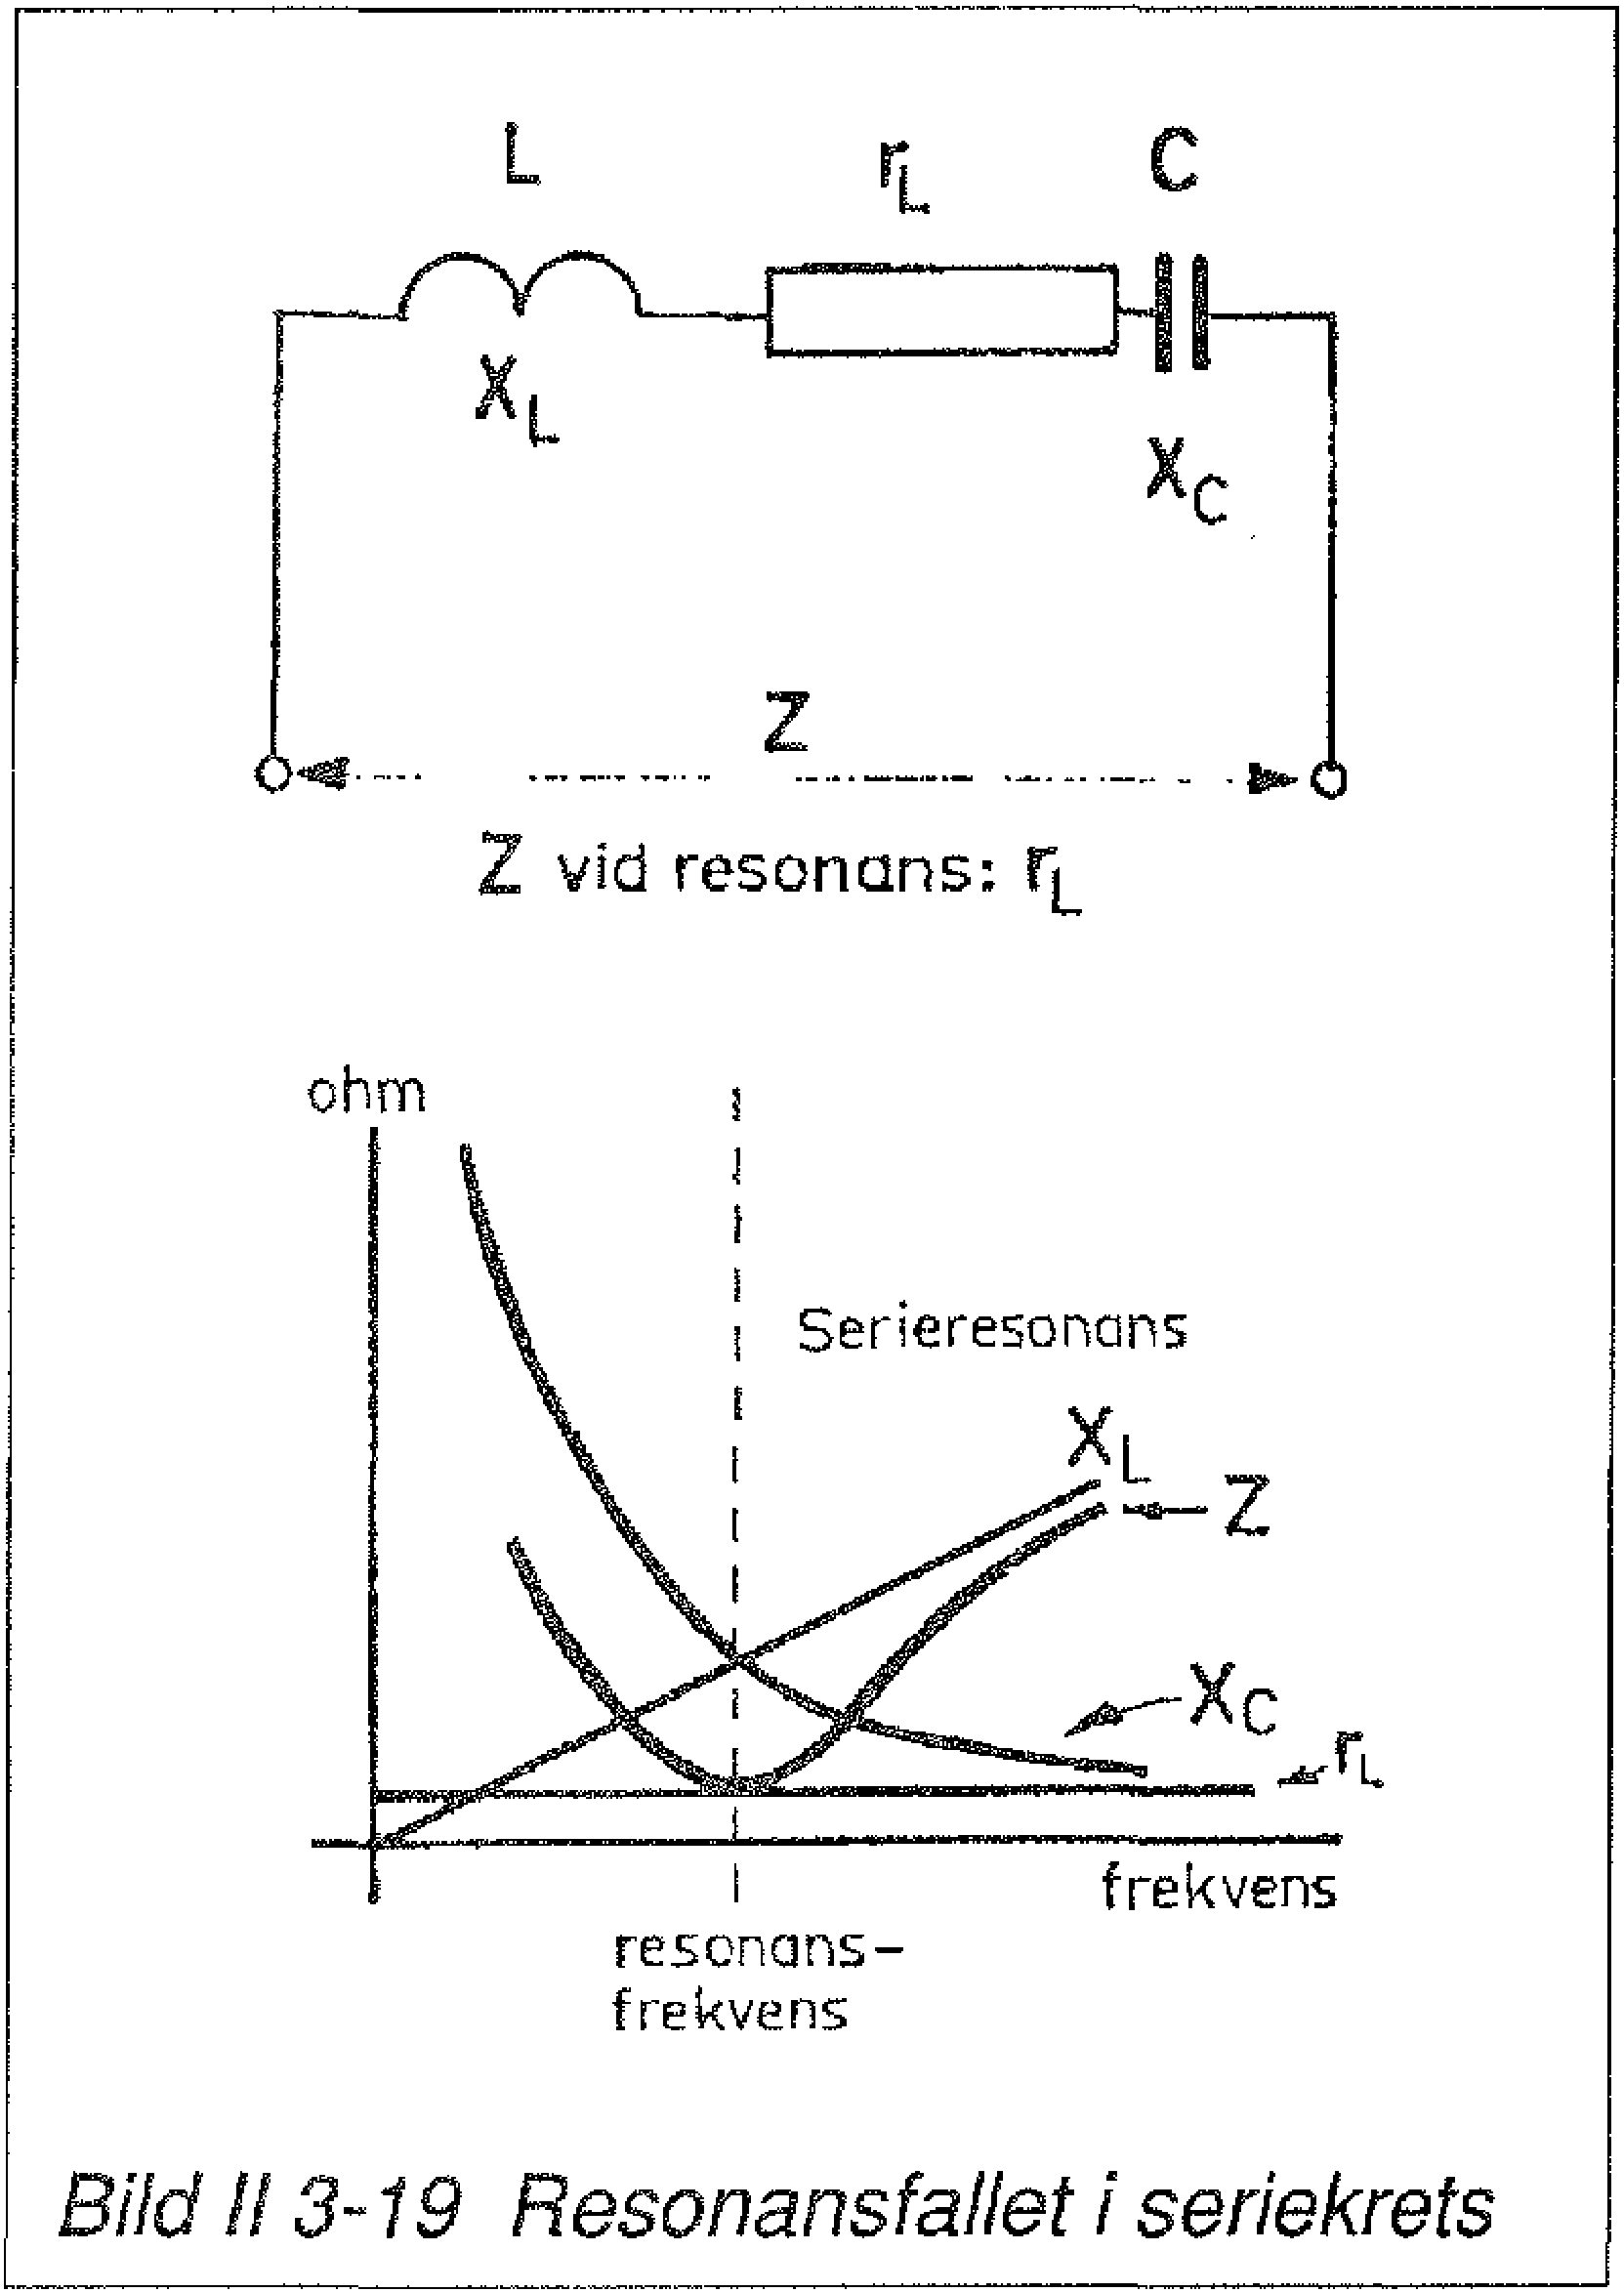
\includegraphics[width=7cm]{images/bild_2_3-19}
\caption{Resonansfallet i seriekrets}
\label{fig:BildII3-19}
\end{center}
\end{figure}

Bild \ref{fig:BildII3-19}

När en seriekrets är i resonans, så är

\begin{align*}
& X_L = X_C \quad & \text{d.v.s.} \quad \omega L = \frac{1}{\omega C} \\
& \text{eller} & \\
& X_L - X_C = 0 \quad & \text{d.v.s.} \quad \omega L - \frac{1}{\omega C} = 0
\end{align*}

Med ovanstående kretsdata blir Z = 100 kΩ.

Därav framgår, att impedansen i parallellkretsen är en funktion av det s.k.
L/C-förhållandet samt av kretsens resistiva förluster.

Med ovanstående kretsdata blir resonansfrekvensen:

\[
f_0 = \frac{1}{2π\sqrt{LC}} \approx 796\ kHz
\]

Vid resonansfrekvensen blir reaktansen 1000 Q både i induktansen och
kapacitansen. Eftersom reaktansernas spänningsfall är motriktade tar de ut
varandra. Kretsens impedans i resonans blir resistansen \(r_L\) och
spänningsfallet över kretsen bestäms enbart av \(r_L\).

Antag att det alstras en spänning av 5 mV i antennkretsen. Strömmen genom den
vid resonans blir då \(\frac{5\ mV}{10\ Ω} = 0.5\ mA\).

Av strömmen bildas reaktiva spänningar, d.v.s.
\(0.5 mA \cdot 1000\ Ω = 500\ mV\) både över induktans och kapacitans (som tar
ut varandra) och 5 mV över resistansen.

\subsection{Q-faktorn i en parallellkrets}
\textbf{HAREC a.\ref{HAREC.a.3.2.5}\label{myHAREC.a.3.2.5}}

Bild II 3-20

Godhetstalet Q (=Quality Factor) kan ses som den förmåga en svängningskrets har
att lagra energi, d.v.s. förhållandet mellan den lagrade energin och
energiförlusten i kretsen. Energiförlusten yttrar sig som värmeutveckling.

\[
Q = 2π\frac{\text{lagrad energi i kretsen}}{\text{energiförlusten per period}}
\]

Energiförluster uppstår både i kretsens kondensator och induktor, men moderna
kondensatorer har så låga förluster att induktorn ensam kan anses bestämma
Q-värdet, åtminstone i kortvågsområdet.

En växelspänning \(U_1\) ansluts till en parallellkrets. I resonansfallet
uppträder då en spänning \(U_2\) över kondensatorn och induktorn.

\(U_2\) är mycket större än \(U_1\). Ju högre \(Q\) är i kretsen desto större är
förhållandet mellan \(U_2\) och \(U_1\).

I kortvågsområdet är det vanligt med ett \(Q\) i storleksordningen 30 - 100.
Ju högre Q är, desto mindre är bandbredden.

När svängningskretsen är i resonans gäller sambandet

\[Q = \frac{f_{res}}{b}\]

Bandbredden ökar (avstämningsskärpan minskar) vid ökande frekvens på grund av de
större kretsförlusterna.

Bild II 3-20 Q-värden i parallellkrets
\textbf{HAREC a.\ref{HAREC.a.3.2.6}\label{myHAREC.a.3.2.6}}

\subsection{Bandbredd}

Bild II 3-21

Bilden visar med en kurva vilket impedansvärde kretsen har vid olika frekvenser.
Impedansens högsta värde är vid frekvensen \(f_{res}\) och avtar vid frekvenser
som är högre eller lägre. Vid frekvenserna \(f_1\) och \(f_2\) är
impedansvärdet t.ex. 70\% av maximalvärdet. Med bandbredden \(b\) förstås
skillnaden mellan impedansvärdena i ett sådant frekvenspar, d.v.s.
\(b = f_2 - f_1\).

Bild II 3-21 Bandbredd i parallellkrets

%\section{Filter}
\textbf{HAREC a.\ref{HAREC.a.3.2}\label{myHAREC.a.3.2}}
\index{filter}
\index{filter!frekvensfilter}

%% sid II3-7/138

Frekvensfilter, eller mer allmänt filter, används inom radiotekniken för många
olika ändamål, t.ex. för att
\begin{itemize}
\item eliminera störande signaler,
\item  öka avstämningsskärpan (selektiviteten) i mottagare och sändare,
\item framhäva eller dämpa ett sidband i en AM-signal m.m.
\end{itemize}

Beroende på den s.k. frekvensgången, så indelas filtren i flera ''familjer'',
varav de vanliga presenteras här.

Beroende på det tekniska utförandet finns dels s.k. passiva filter vilka
använder extern energi för sin funktion, och dels aktiva filter vilka i princip
är förstärkare som likaledes använder passiva kretsar. Här presenteras
för enkelhetens skull passiva filter.

Traditionella frekvensfilter är vad som kallas analoga. Men nu i dataåldern
börjar även digitala filter vinna intåg. Sådana är dock för komplicerade för
att behandlas här.

\subsection{Högpassfilter (HP)}
\textbf{HAREC a.\ref{HAREC.a.3.2.8b}\label{myHAREC.a.3.2.8b}}
\index{högpassfilter}
\index{filter!högpass (HP)}
\index{highpass filter}
\index{HP}

\begin{figure}
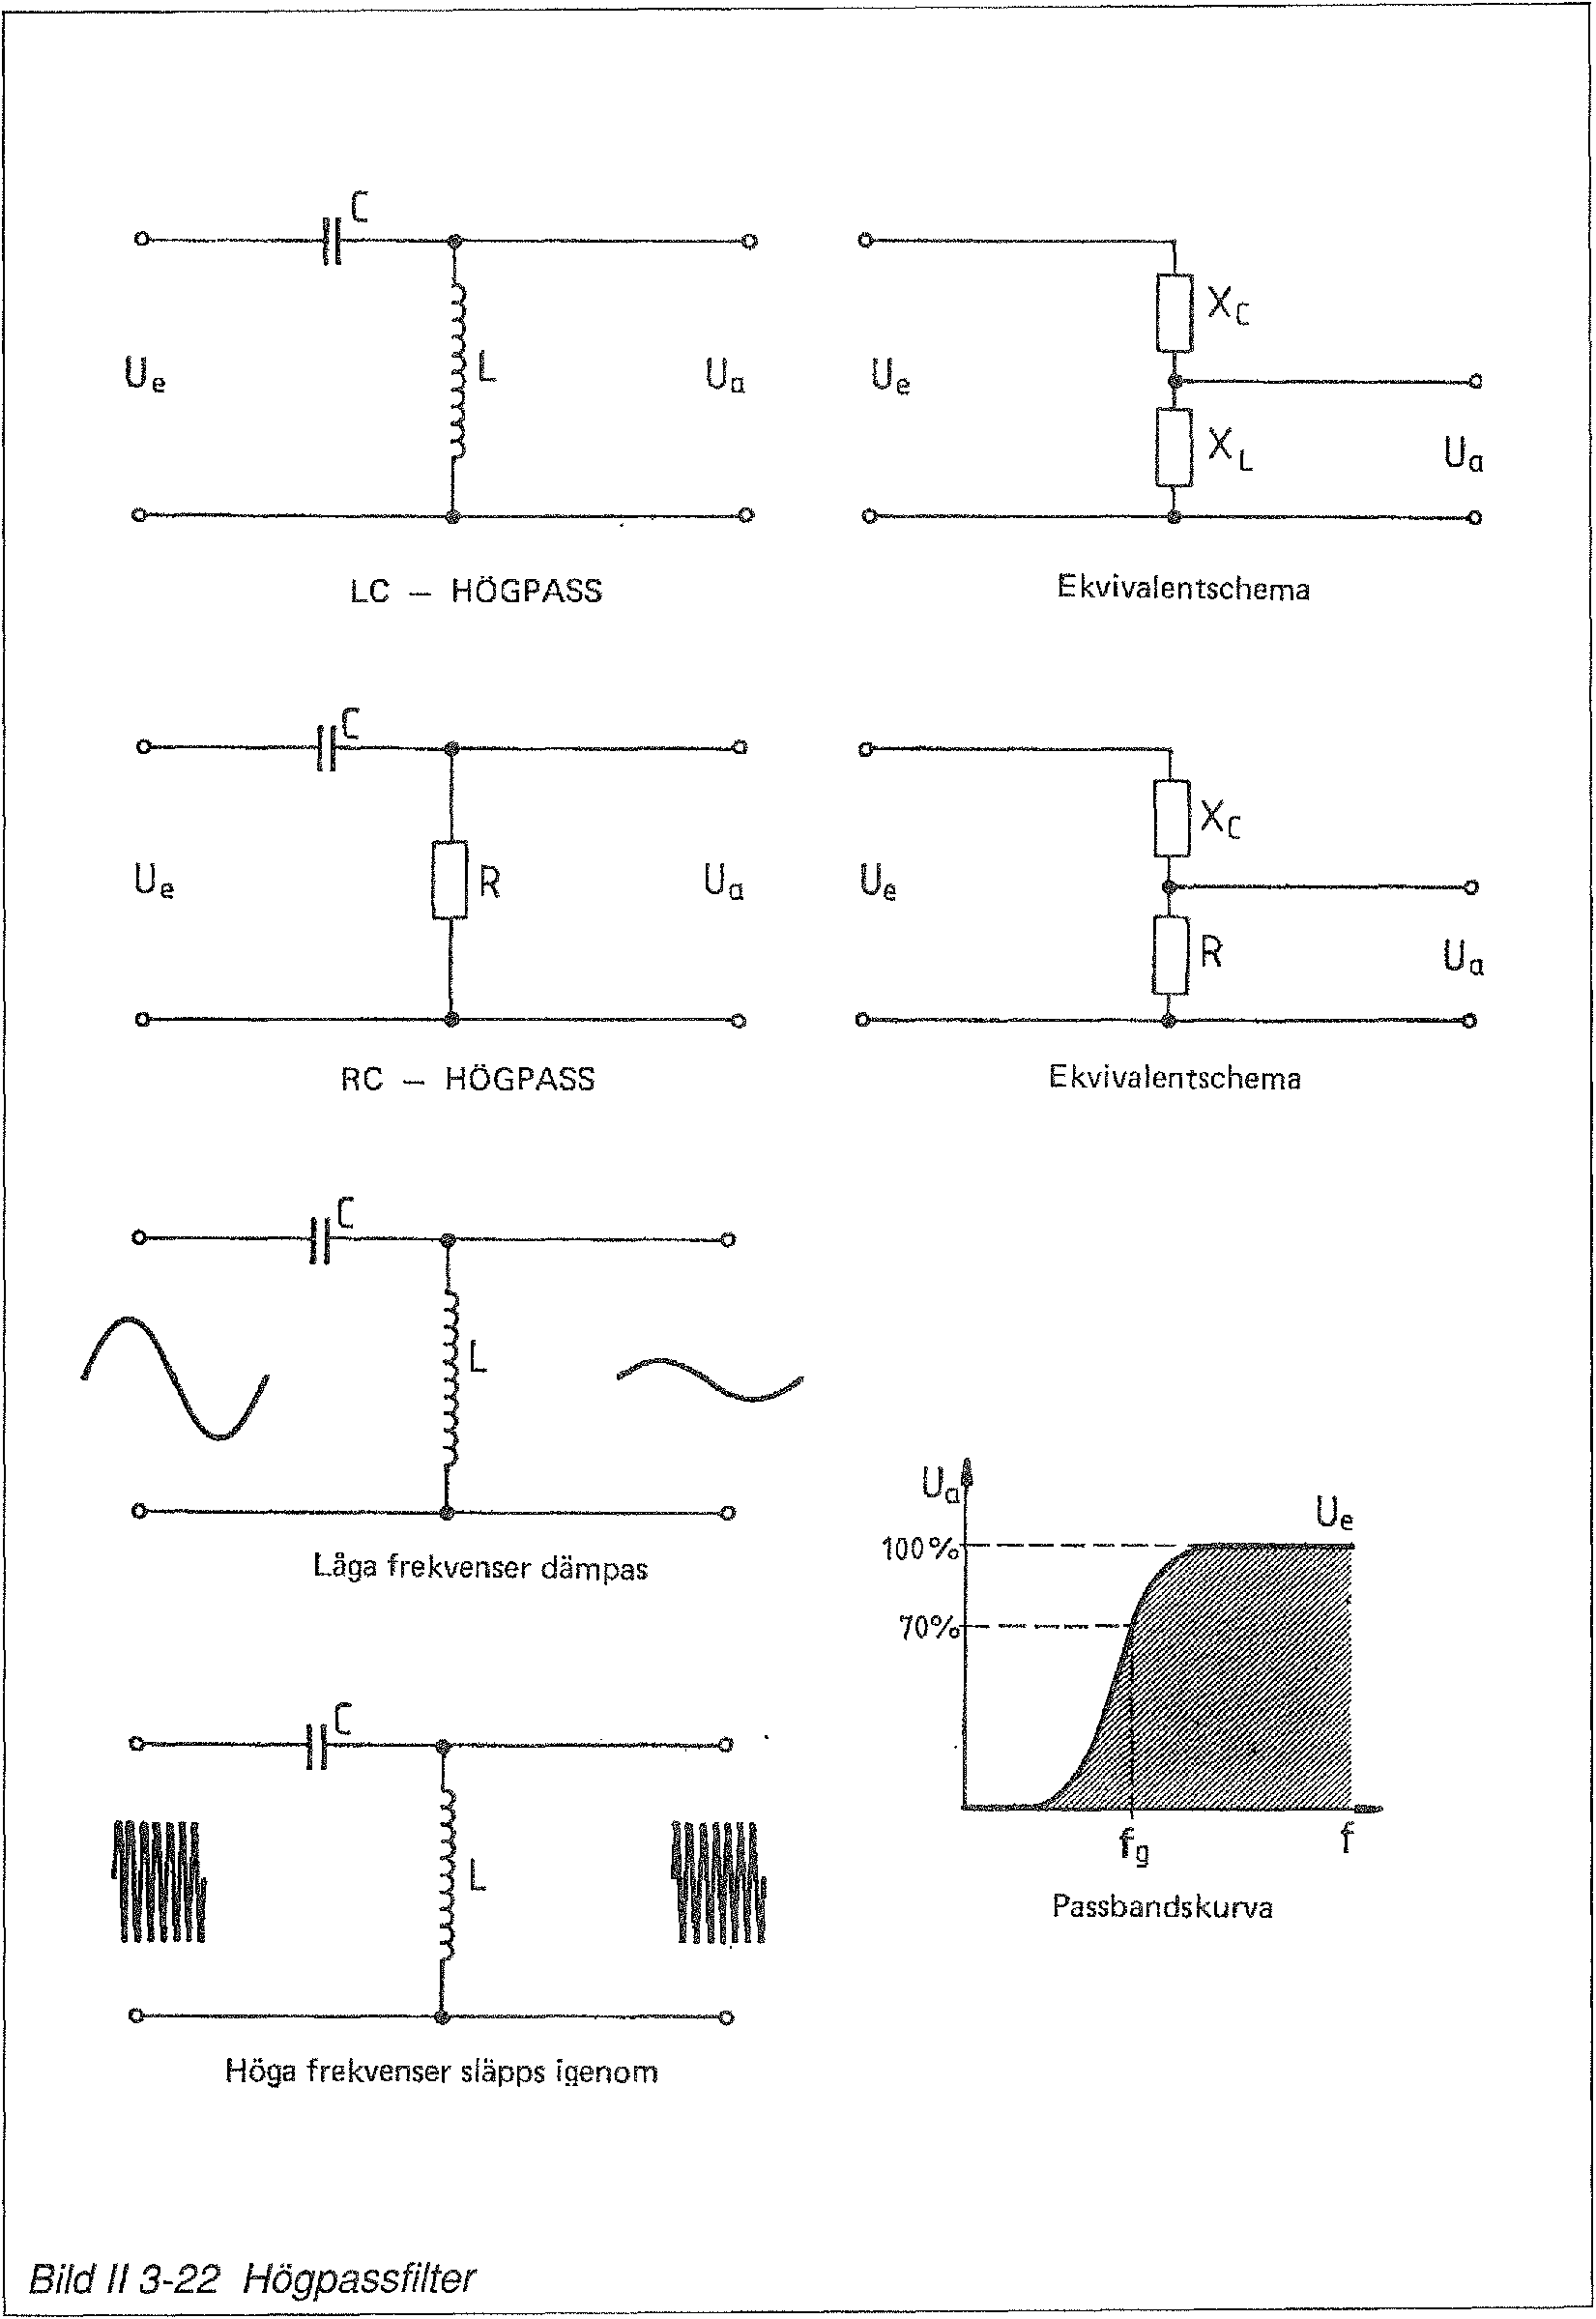
\includegraphics[width=\textwidth]{images/bild_2_3-22.png}
\caption{Högpassfilter}
\label{fig:BildII3-22}
\end{figure}

Bild \ref{fig:BildII3-22}

Ett \emph{högpassfilter} (eng \emph{highpass filter (HP)}) släpper igenom
signaler med höga frekvenser och dämpar dem med låga frekvenser.

Exempel: En frekvensberoende spänningsdelare som LC-högpassfilter.

Vid låga frekvenser är \(X_C\) stor och \(X_L\) liten. Över XL uppstår då ett
litet spänningsfall -- en låg utgångsspänning \(U_a\). Resultatet blir att
låga frekvenser dämpas.

Vid höga frekvenser är \(X_C\) liten och \(X_L\) stor. Över \(X_L\) uppstår då
ett stort spänningsfall -- en hög utgångsspänning \(U_a\). Resultatet blir att
höga frekvenser släpps igenom.

\(X_L\) kan bytas ut mot en resistor \(R\), men då blir passbandkurvan inte så
brant.

\emph{Gränsfrekvens}

Gränsfrekvensen \(f_g\) beror av kapacitansen \(C\), induktansen \(L\) samt
resistansen \(R\).

LC-högpass:
\begin{gather*}
  f_g = \frac{1}{2π\sqrt{LC}} \\
  f_g\ \text{[Hz]} \quad L\ \text{[H]} \quad C\ \text{[F]}
\end{gather*}

RC-Högpass:
\begin{gather*}
  f_g = \frac{1}{2πRC}
  f_g\ \text{[Hz]} \quad R\ \text{[Ω]} \quad C\ \text{[F]}
\end{gather*}

Räkneexempel:
\begin{enumerate}
\item \(L = 4\ \text{H} \quad C = 1\ \text{µF} \quad f_g =\ ?\)
  \[
  f_g = \frac{1}{2π\sqrt{4 \cdot 10^{-6}}} = \frac{500}{2π}
  = 79,6\ \text{Hz}
  \]
\item \(R = 1\ \text{kΩ} \quad C = 10\ \text{nF} \quad f_g =\ ?\)
  \[
    f_g = \frac{1}{2π \cdot 1 \cdot 10^3 \cdot 10 \cdot 10^{-9}}
    = \frac{10^5}{2π} = 15,9\ \text{kHz}
  \]
\end{enumerate}

\subsection{Lågpassfilter (LP)}
\textbf{HAREC a.\ref{HAREC.a.3.2.8a}\label{myHAREC.a.3.2.8a}}
\index{lågpassfilter}
\index{filter!lågpass (LP)}
\index{lowpass filter}
\index{LP}

\begin{figure}
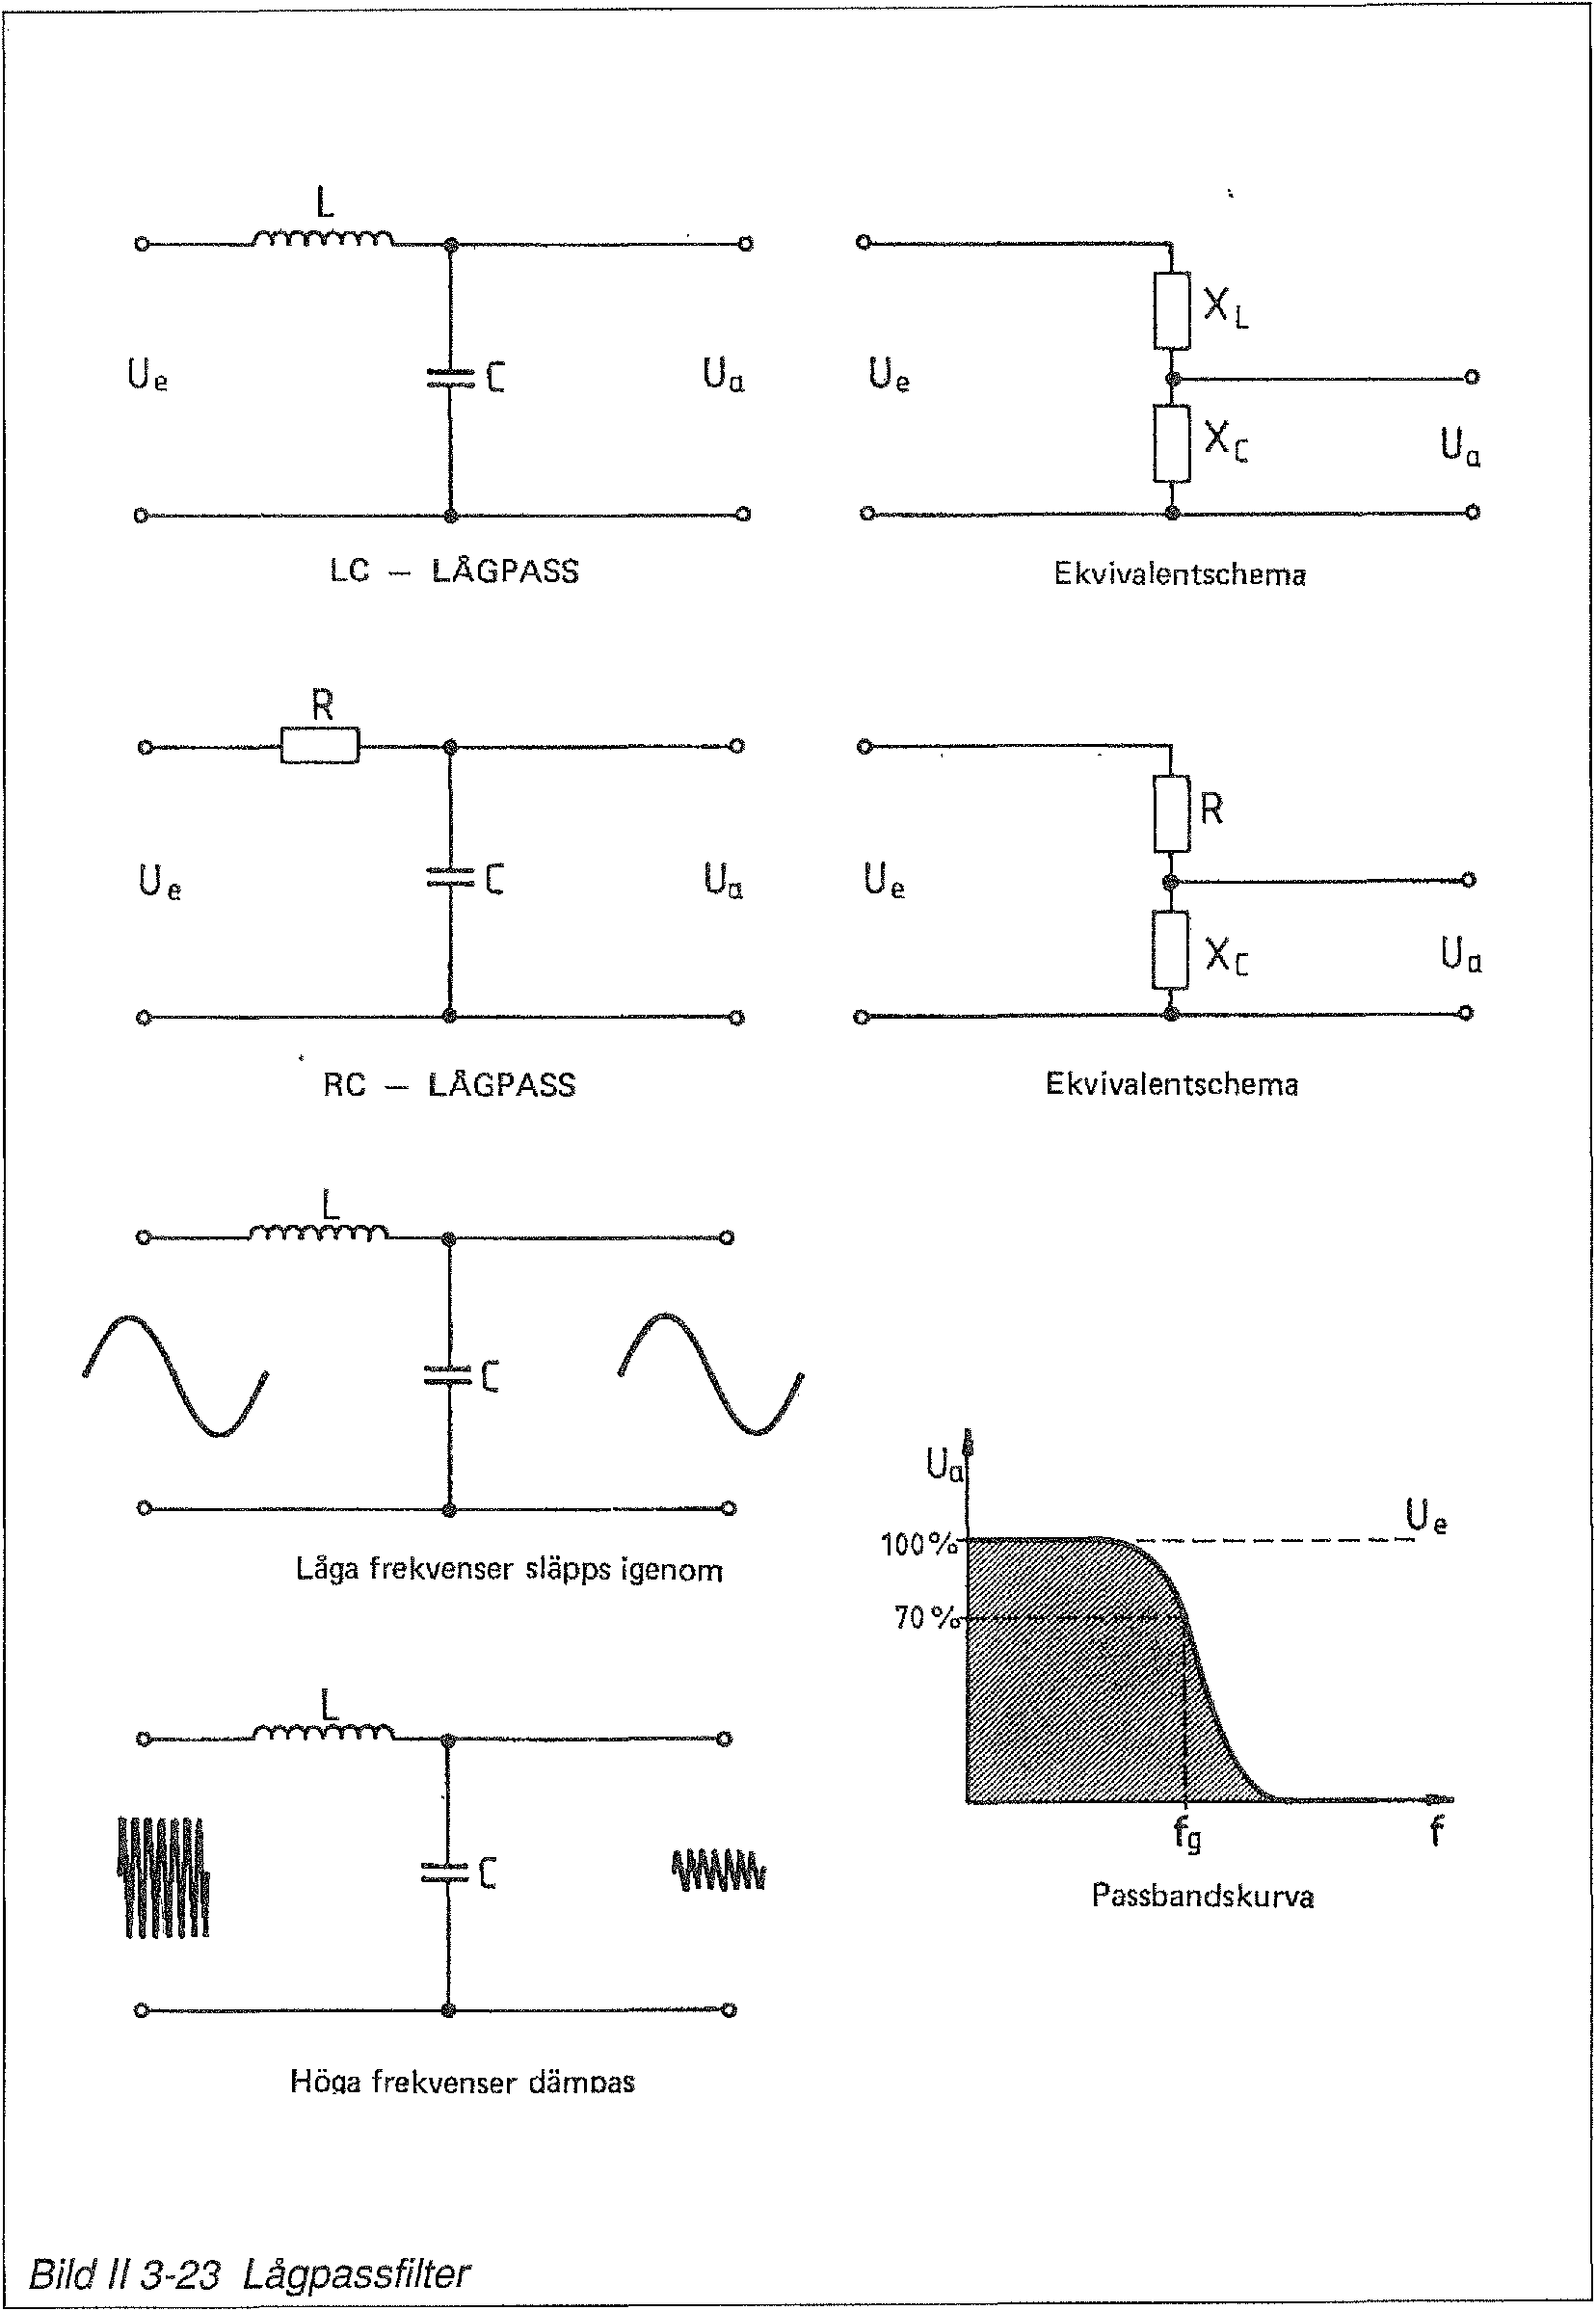
\includegraphics[width=\textwidth]{images/bild_2_3-23.png}
\caption{Lågpassfilter}
\label{fig:BildII3-23}
\end{figure}

Bild \ref{fig:BildII3-23}

Om induktor och kondensator respektive resistor och kondensator i ett
högpassfilter byter plats, så får man i stället ett LC-lågpassfilter respektive
ett RC-lågpassfilter.

Ett \emph{lågpassfilter} (eng \emph{lowpass filter (LP)}) släpper igenom
signaler med låga frekvenser och dämpar dem med höga frekvenser.

Exempel: En frekvensberoende spänningsdelare som LC-Lågpassfilter.

Vid låga frekvenser är \(X_C\) stor och \(X_L\) liten. Över \(X_L\) uppstår då
ett litet spänningsfall -- en hög utgångsspänning \(U_a\). Resultatet blir att
låga frekvenser släpps igenom.

Vid höga frekvenser är \(X_C\) liten och \(X_L\) stor. Över \(X_L\) uppstår då
ett stort spänningsfall -- en låg utgångsspänning \(U_a\). Resultatet blir att
höga frekvenser dämpas.

\emph{Gränsfrekvens}

Samma formler används vid beräkning av gränsfrekvensen både i lågpass- och
högpassfilter, således

LC-Lågpass:
\begin{gather*}
  f_g = \frac{1}{2π\sqrt{LC}} \\
  f_g\ \text{[Hz]} \quad L\ \text{[H]} \quad C\ \text{[F]}
\end{gather*}

RC-Lågpass:
\begin{gather*}
  f_g = \frac{1}{2π{RC}} \\
  f_g\ \text{[Hz]} \quad R\ \text{[Ω]} \quad C\ \text{[F]}
\end{gather*}

\subsection{Bandpassfilter (BP)}
\textbf{HAREC a.\ref{HAREC.a.3.2.8c}\label{myHAREC.a.3.2.8c}}
\index{bandpassfilter}
\index{filter!bandpass (BP)}
\index{bandpass filter}
\index{BP}

\begin{figure}
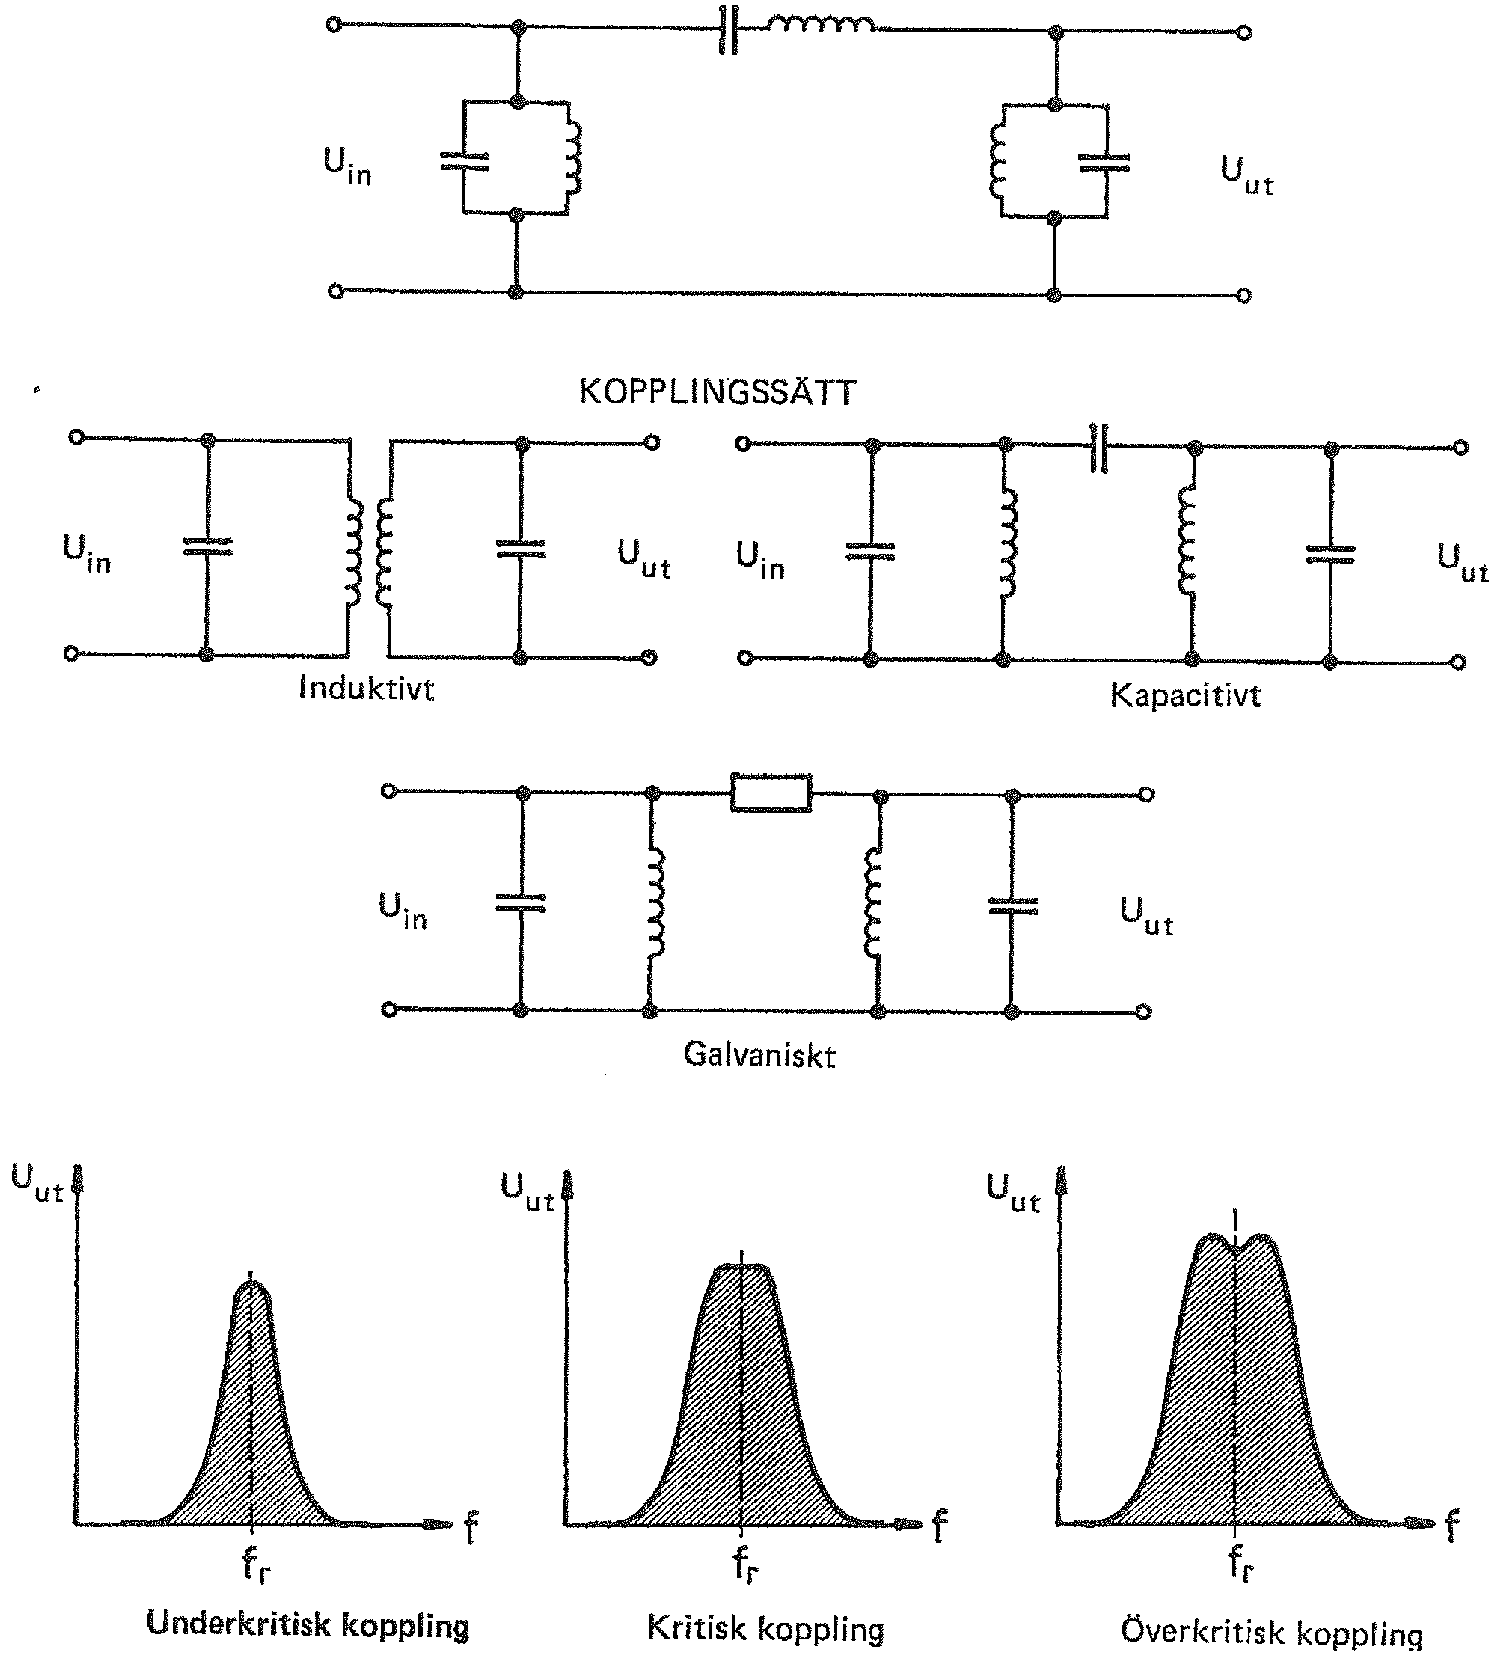
\includegraphics[width=\textwidth]{images/bild_2_3-24.png}
\caption{Bandpassfilter}
\label{fig:BildII3-24}
\end{figure}

Bild \ref{fig:BildII3-24}

Ett bandpassfilter släpper igenom signaler bara inom ett frekvensområde medan
signaler inom andra frekvensområden dämpas.

Bandpassfiltret består i enklaste fall av två svängningskretsar av LC-typ, vilka
är avstämda till angränsande frekvenser. Kretsarna är kopplade induktivt,
kapacitivt eller galvaniskt.

Beroende på kopplingsgrad skiljer man mellan underkritisk koppling (lös
koppling), kritisk koppling och överkritisk koppling (fast koppling).

På bilden visas hur passbandet påverkas bl.a. av kopplingsgraden. Lös koppling
liten bandbredd. Kritisk koppling -- större bandbredd. Fast koppling -- stor
bandbredd.

\subsection{Passfilter}
\index{passfilter}
\index{filter!bandpass (BP)}
\index{pass filter}
\index{BP}

\begin{figure}
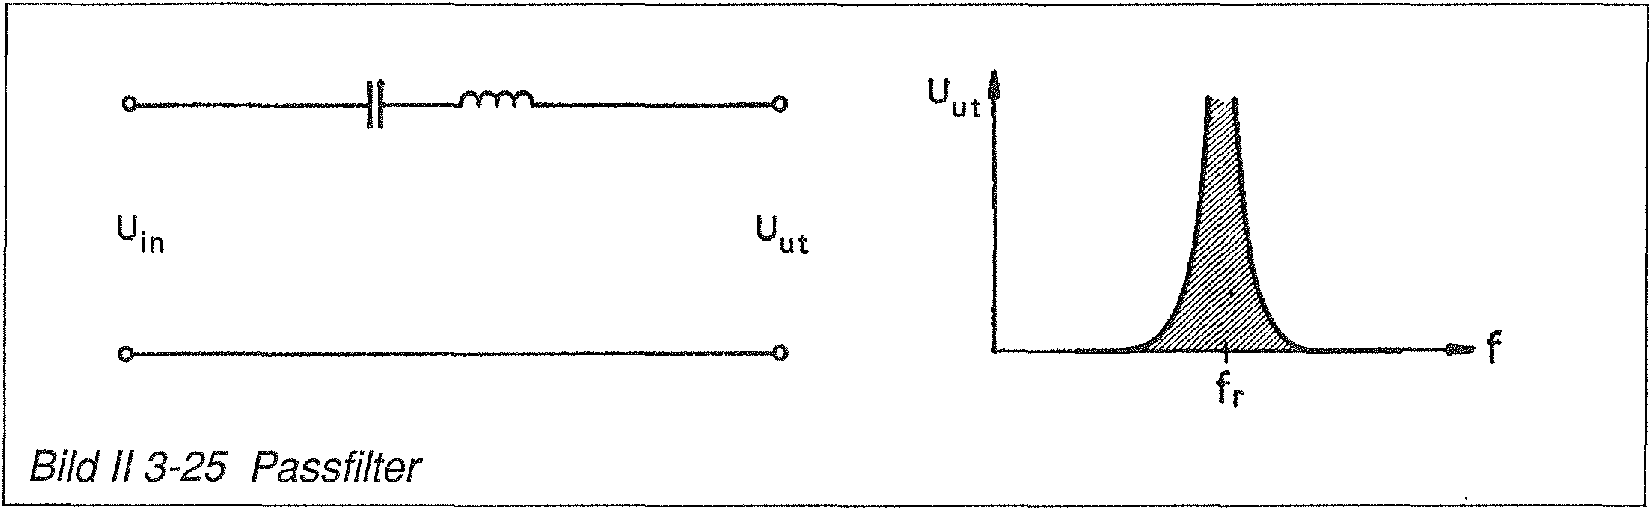
\includegraphics[width=\textwidth]{images/bild_2_3-25.png}
\caption{Passfilter}
\label{fig:BildII3-25}
\end{figure}

Bild \ref{fig:BildII3-25}

Passkretsen stäms av till en viss frekvens och erbjuder där en mycket låg
impedans. Passkretsen kopplas i serie med signalvägen och låter signaler med
frekvenser inom filtrets passband att passera.

\subsection{Bandspärrfilter}
\textbf{HAREC a.\ref{HAREC.a.3.2.8d}\label{myHAREC.a.3.2.8d}}
\index{bandspärrfilter}
\index{filter!bandspärr (BR)}
\index{band reject filter (BR)}
\index{BR}

\begin{figure}
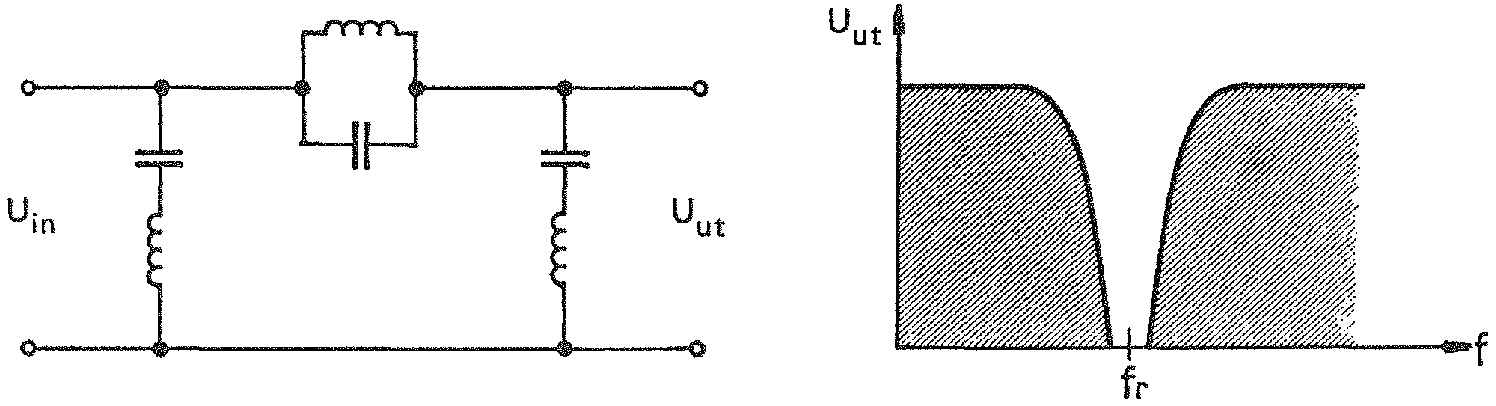
\includegraphics[width=\textwidth]{images/bild_2_3-26.png}
\caption{Bandspärrfilter}
\label{fig:BildII3-26}
\end{figure}

Bild \ref{fig:BildII3-26}

Om serie- och parallellkretsarna i ett bandpassfilter byter plats, så får man
i stället ett bandspärrfilter. Ett sådant spärrar signaler inom ett visst
frekvensområde, men släpper igenom signaler utom detta område.

\subsection{Spärrfilter}
\index{spärrfilter}
\index{filter!spärr (BR)}
\index{band reject filter (BR)}
\index{BR}
\index{spärrkrets}
\index{sugkrets}

\begin{figure}
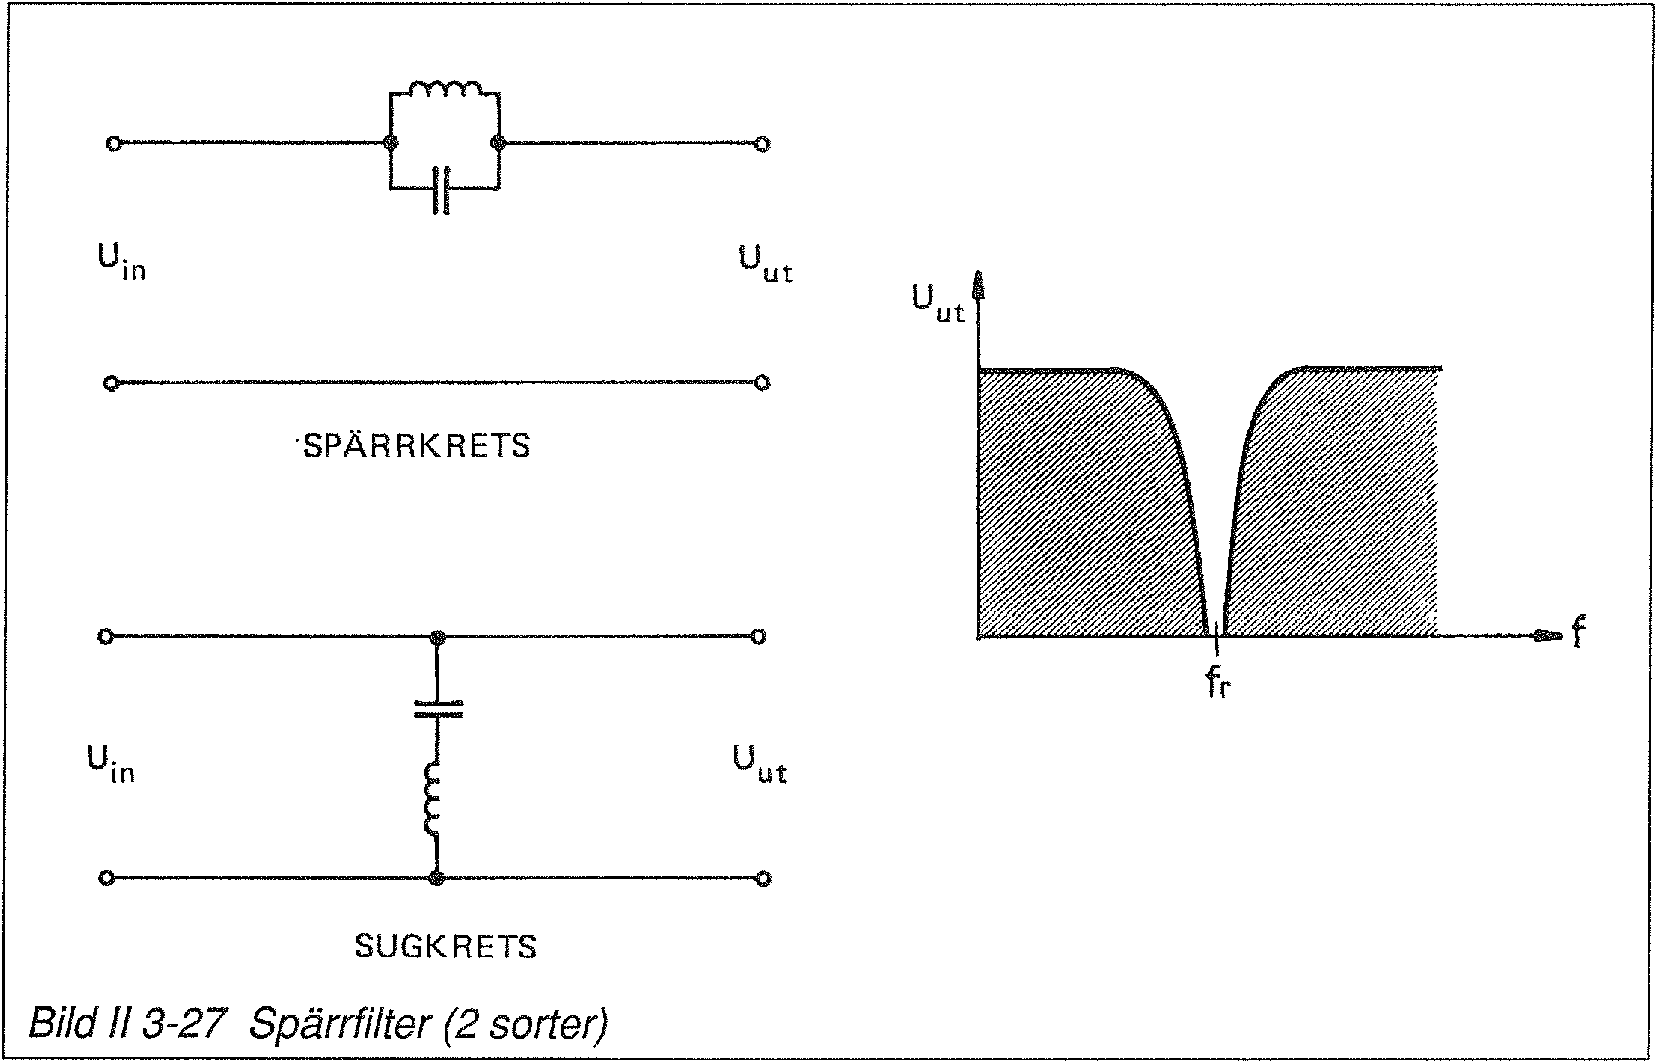
\includegraphics[width=\textwidth]{images/bild_2_3-27.png}
\caption{Spärrfilter (2 sorter)}
\label{fig:BildII3-27}
\end{figure}

Bild \ref{fig:BildII3-27}

\emph{Spärrkrets} \\
Spärrkretsen stäms av till en viss frekvens och erbjuder där en mycket hög
impedans. Spärrkretsen kopplas i serie med signalvägen och spärrar en signal
med samma frekvens som resonansfrekvensen.

Bild \ref{fig:BildII3-27}

\emph{Sugkrets} \\
Sugkretsen stäms av till en viss frekvens och erbjuder där en mycket låg
impedans. Sugkretsen kopplas parallellt med signalvägen och kortsluter (suger
bort) en signal med samma frekvens som resonansfrekvensen.

\begin{wrapfigure}[14]{R}{0.5\textwidth}
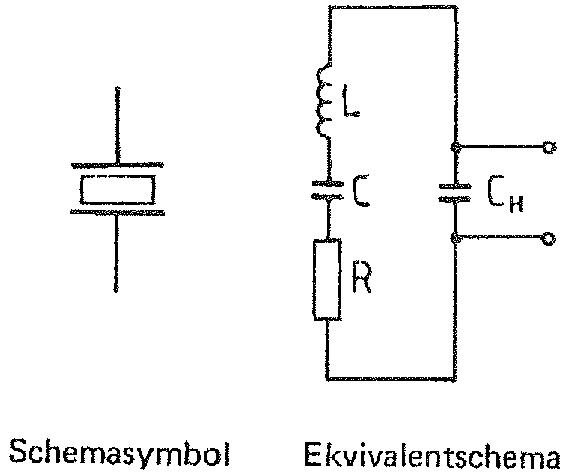
\includegraphics[width=0.5\textwidth]{images/bild_2_3-28.png}
\caption{Kvartskristall}
\label{fig:BildII3-28}
\end{wrapfigure}

\subsection{Kvartskristall}

\textbf{HAREC a.\ref{HAREC.a.3.2.11}\label{myHAREC.a.3.2.11}}
\index{kvartskristall}
\index{quartz crystal}
\index{crystal}
\index{Q-värde}
\index{resonator}

Bild \ref{fig:BildII3-28}

En \emph{kvartskristall} (eng \emph{quartz crystal} eller \emph{crystal}),
egentligen en slipad skiva av kvarts, kan fungera som en
elektromekanisk svängningskropp (resonator), vars egenskaper liknar dem i en
LC-krets.

Den låga inre resistansen gör att Q-värdet i en kvartskristall är bättre än
10000. Som jämförelse är Q-värdet i en LC-krets oftast sämre än 1000.

Många moderna kvartskristaller kan uppvisa olastat Q-värde på 100000.

\vspace{12pt} % Undgår brytning av nästa titelrad

\subsection{Bandfilter med kvartskristaller}
\index{kristallfilter}
\index{crystal filter}
\index{keramiska resonatorer}
\index{ceramic resonators}

\begin{wrapfigure}[17]{R}{0.5\textwidth}
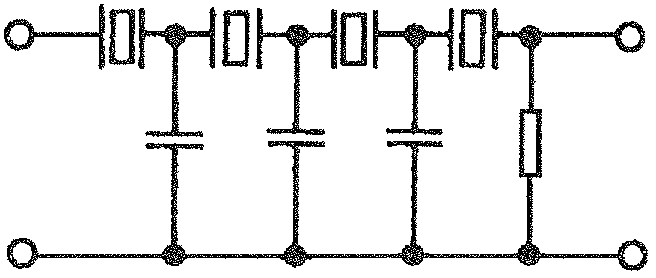
\includegraphics[width=0.5\textwidth]{images/bild_2_3-29.png}
\caption{Bandfilter med kvartskristaller}
\label{fig:BildII3-29}
\end{wrapfigure}

Bild \ref{fig:BildII3-29}

Kvartskristaller kan kombineras till filter, ofta refererade till som
\emph{kristallfilter} (eng \emph{crystal filter}), med önskad bandbredd. Även
utföranden med \emph{keramiska resonatorer} (eng \emph{ceramic resonators})
finns. Resonatorerna är avstämda till var sin bestämda frekvens och hela
komplexet bidrar på så sätt till att bilda passband eller andra egenskaper på
samma sätt som med sammankopplade LC-kretsar.

\subsection{Mekaniska filter}
\index{mekaniskt filter}
\index{mechanical filter}
\index{mekanisk resonator}
\index{resonator!mekanisk}

Bild \ref{fig:BildII3-30}

Med en elektromekanisk givare kan man få en kropp (resonator) att svänga på sin
resonansfrekvens. Med ännu en elektromagnetisk givare kan man känna av
svängningarna och återvandla dem till elektriska signaler. Hela anordningen
fungerar som en \emph{elektromekanisk resonator} (eng
\emph{mechanical resonator}), vars egenskaper liknar dem i en LC-krets.

\begin{figure}
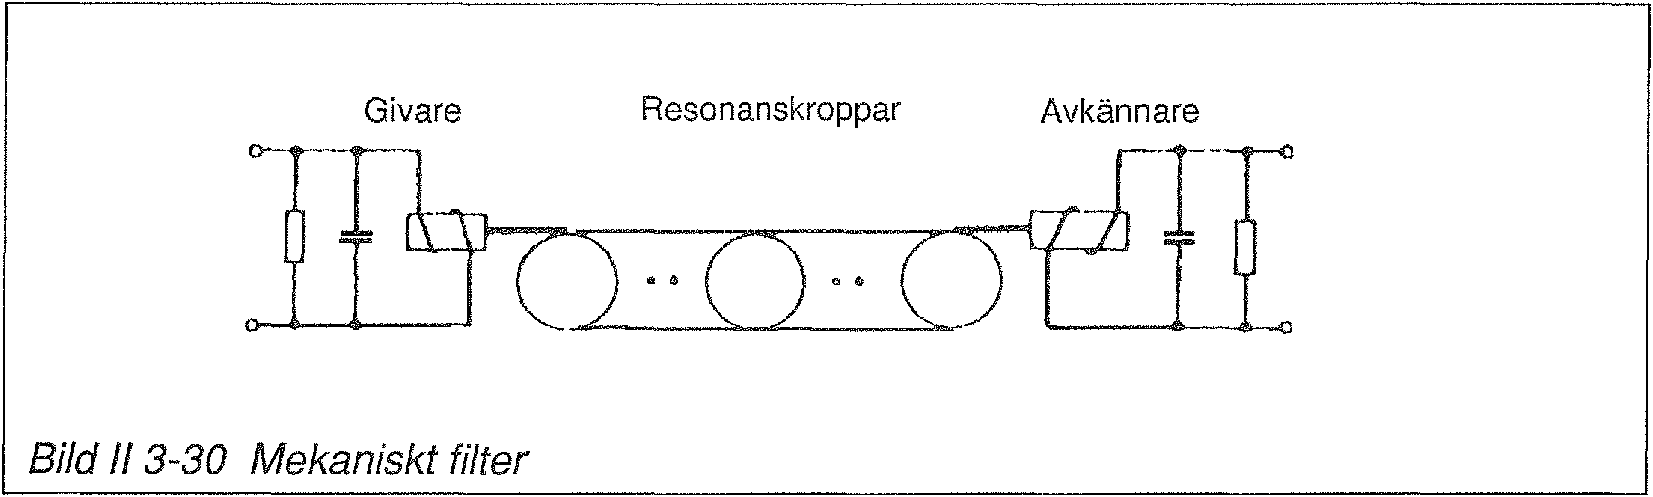
\includegraphics[width=\textwidth]{images/bild_2_3-30.png}
\caption{Mekaniskt filter}
\label{fig:BildII3-30}
\end{figure}

Resonatorerna kan kombineras till filterkomplex med önskad bandbredd där
resenatorerna är avstämda till var sin bestämda frekvens. Hela komplexet bidrar
på så sätt till att bilda ett passband på samma sätt som med sammankopplade
LC-kretsar. Beroende på tillämpningen finns olika frekvenslägen i intervallet
60--600~kHz.

\emph{Mekaniska filter} (eng \emph{mechanical filter}) användes mest förr som
mellanfrekvensfilter i högvärdiga radioutrustningar, men har numera till stor
del ersatts av bandfilter med kvartskristaller där arbetsområdet kan ligga
avsevärt högre i frekvens.

\subsection{Kavitetsfilter}
\index{kavitetsfilter}
\index{cavity filter}
\index{filter!kavitet}

\begin{wrapfigure}[15]{R}{0.5\textwidth}
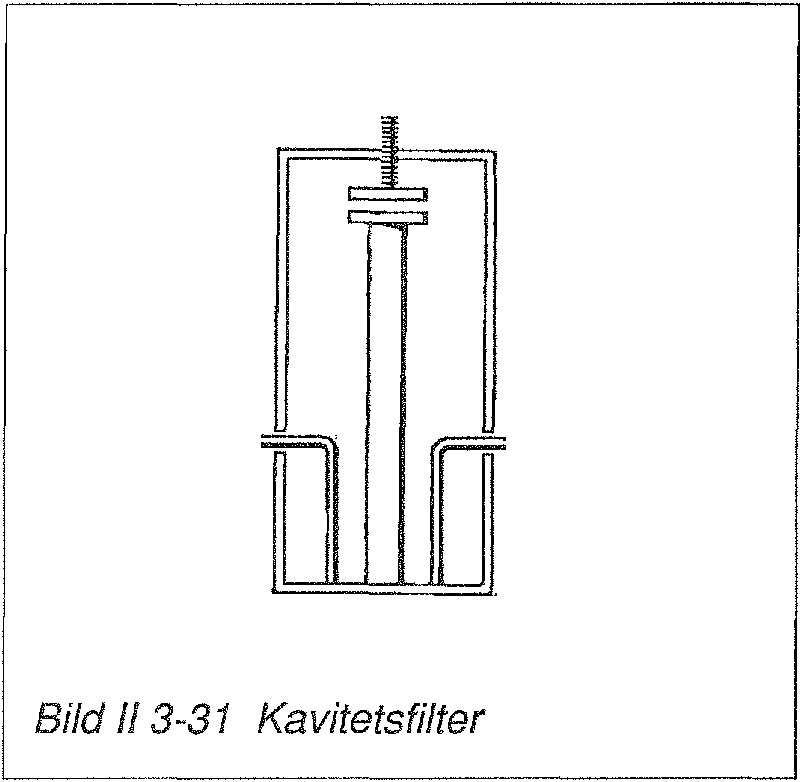
\includegraphics[width=0.5\textwidth]{images/bild_2_3-31.png}
\caption{Kavitetsfilter}
\label{fig:BildII3-31}
\end{wrapfigure}

Bild \ref{fig:BildII3-31}

Svängningskretsars dimensioner minskar med ökande frekvens. Vid mycket hög
frekvens kan induktorns varvtal i en LC-krets ha minskat till ett enda varv
samtidigt som kapacitansen inom detta enda varv kan räcka för önskad
resonansfrekvens.

En sådan svängningskrets kan bl.a. ha formen av en ledare mitt inne i en
elektriskt ledande kavitet. Ledarens längd tillsammans med kavitetens insida
bildar induktorn. Mellan ledaren och kavitetens insida råder en kapacitans,
som kan kompletteras/justeras med en extra kondensator.

Inkommande och utgående signaler ansluts till filtrets mittledare över
induktionsslingor, kondensatorer eller direkt galvaniskt. \emph{Kavitetsfilter} (eng
\emph{cavity filter}) kan kopplas ihop för att bilda bandfilter, frekvensdelare
m.m.

\subsection{Helixfilter}
\index{helixfilter}
%\index{helix filter}
\index{filter!helix}

När ett kompakt kavitetsfilter behövs, så kan man öka reaktansen i mittledaren
både induktivt och kapacitivt genom att utforma den som en spiral (helix).
Detta är dock på bekostnad av Q-värdet. Flera kavitetsfilter kan kopplas ihop
för att bilda bandfilter, spärrfilter m.m.

\subsection{Pi-filter}
\textbf{HAREC a.\ref{HAREC.a.3.2.10a}\label{myHAREC.a.3.2.10a}}
\index{Pi-filter}
\index{filter!Pi-filter}

\begin{wrapfigure}[16]{R}{0.5\textwidth}
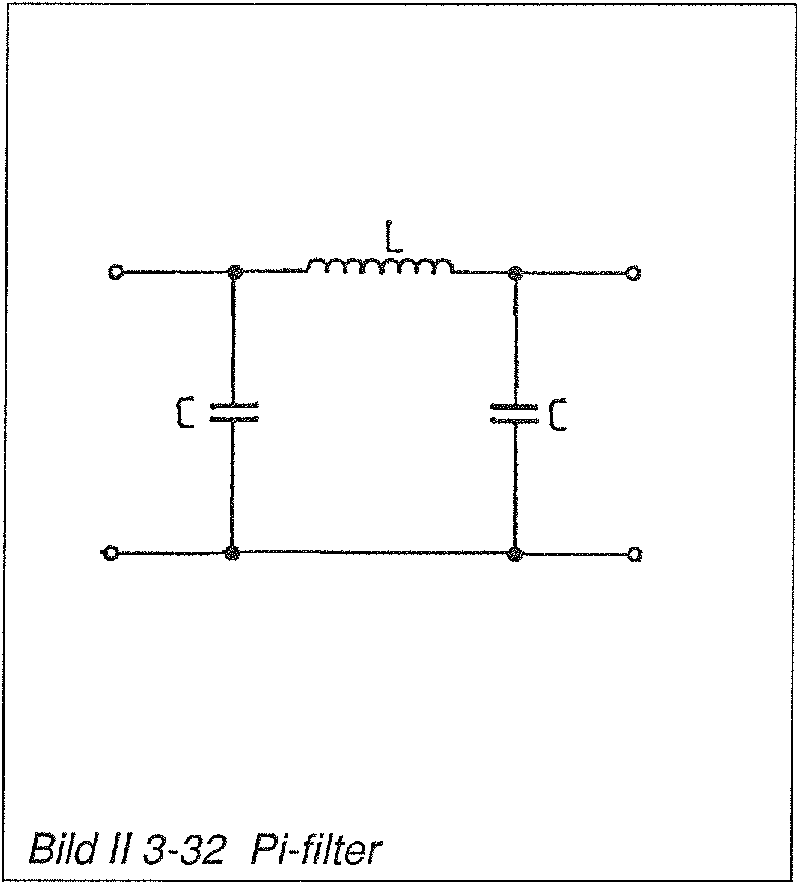
\includegraphics[width=0.5\textwidth]{images/bild_2_3-32.png}
\caption{Pi-filter}
\label{fig:BildII3-32}
\end{wrapfigure}

Bild \ref{fig:BildII3-32}

För att överföra HF-signaler med bästa verkningsgrad, så är det viktigt med god
impedansanpassning mellan de olika funktionerna. Om anslutningsimpedansen är
lika i båda funktionerna, så behövs inga extra åtgärder. Är impedanserna däremot
olika, så behövs korrigeringsnät (filter).

Ofta är nätet Pi-format och består av induktanser och kapacitanser. Ett
Pi-format nät kan sägas bestå av två L-formade nät ställda mot varandra, där
den seriella delen är gemensam (på bilden en induktor).

\subsection{T-filter}
\textbf{HAREC a.\ref{HAREC.a.3.2.10b}\label{myHAREC.a.3.2.10b}}
\index{T-filter}
\index{filter!T-filter}

\begin{wrapfigure}[16]{R}{0.5\textwidth}
\includegraphics[width=0.5\textwidth]{images/bild_2_3-33.png}
\caption{T-filter}
\label{fig:BildII3-33}
\end{wrapfigure}

Bild \ref{fig:BildII3-33}

Ett nät kan också vara T-format och bestå av induktanser och kapacitanser. Ett
sådant nät kan sägas bestå av två L-formade nät ställda ''rygg mot rygg''. Då är
den parallella delen gemensam. På bilden visas två alternativ.

När den parallella delen är kapacitiv, blir huvudkaraktären ett lågpassfilter,
men att impedansanpassning också är möjlig med en induktiv impedansdelning.

När den parallell delen är induktiv blir huvudkaraktären ett högpassfilter, men
att impedansanpassning också är möjlig med en kapacitiv impedansdelning.

Ett Pi- eller T-filter kan fungera som
\begin{itemize}
\item svängningskrets,
\item impedanstransformator (anpassning),
\item balansera ut en reaktans o.s.v.
\end{itemize}

%\section{Kraftförsörjning}
\textbf{HAREC a.\ref{HAREC.a.3.3}\label{myHAREC.a.3.3}}
\label{kraftaggregat}
\index{kraftförsörjning}
\index{kraftaggregat}
\index{batteri}
\index{ackumulator}

Den elektriska energi, som behövs för elektronikutrustningar, hämtas
från det allmänna elektricitetsnätet, ett batteri eller en
ackumulator.
Vissa batterityper kan återuppladdas och kallas då ackumulator.

Batterier och ackumulatorer avger en nominell spänning, som beror av
de ingående materialen och givetvis av laddningstillståndet.
Moderna utrustningar för amatörradio är utförda för 12~V likström och försörjs
vanligen från ett nätanslutet kraftaggregat.
På så sätt kan mobila radioutrustningar även försörjas från startackumulatorn
i fordonet.

Handburna radioutrustningar försörjs från en inbyggd ackumulator, som
laddas från stationär laddare.

Äldre stationära radioutrustningar drivs nästan alltid med nätanslutna
kraftaggregat med en eller flera transformatorer och likriktare.
Alternativt kan samma transformators sekundärsida vara
försedd med flera lindningar för olika spänningar och strömkretsar.

Det allmänna elnätet i Sverige levererar växelspänning med frekvensen 50~Hz.
Nätspänningen för hushållsändamål är numera 400/230~V.

Tidigare importerade utrustningar i marknaden kan vara utförda för andra
nätspännings- och skyddsjordningssystem än vad som nu tillämpas i Sverige.
Försiktighet med sådan utrustning rekommenderas.

\subsection{Halv- och helvågslikriktning m.m.}
\textbf{HAREC a.\ref{HAREC.a.3.1.1g}\label{myHAREC.a.3.1.1g}, a.\ref{HAREC.a.3.3.1}\label{myHAREC.a.3.3.1}}
\index{likriktning}
\index{rectifier}

\begin{wrapfigure}{R}{0.5\textwidth}
\includegraphics[width=0.5\textwidth]{images/cropped_pdfs/bild_2_3-34.pdf}
\caption{Halvledardioder}
\label{fig:BildII3-34}
\end{wrapfigure}

\emph{Likriktning} (eng. \emph{rectificiation}) av spänningar och strömmar i en
krets görs med ''elektroniska ventiler'', som släpper igenom ström endast i den
s.k. passriktningen och stoppas i spärriktningen så som illustreras i bild
\ref{fig:BildII3-34}.
En sådan strömventil kallas för diod och kan vara av typen vakuumrör eller
halvledare.
I moderna konstruktioner används uteslutande halvledardioder i
likriktarkopplingar.

\begin{figure}
\includegraphics[width=\textwidth]{images/cropped_pdfs/bild_2_3-35.pdf}
\caption{Halv- och helvågslikriktning}
\label{fig:BildII3-35}
\end{figure}

\subsubsection{Halvvågslikriktning}
\index{halvvågslikriktning}
\index{likriktning!halvvågs}

Vid \emph{halvvågslikriktning} (eng. \emph{half wave rectifier}) släpps endast
varannan halvvåg av en växelspänning igenom.
I den strömkrets, som bildas av transformatorns sekundärlindning, dioden och
belastningen, flyter därför ström endast under varannan halvperiod, så som
illustreras i bild \ref{fig:BildII3-35}.

\subsubsection{Helvågslikriktning}
\index{helvågslikriktning}
\index{likriktning!helvågs}
\index{Graetz-brygga}
\index{likriktning!Graetz-brygga}

I följande kopplingar med två respektive fyra dioder släpps varje halvvåg av
transformatorns växelspänning igenom så att alla halvvågor får samma polaritet.
Ström flyter genom belastningen i samma riktning nder varje halvperiod.
Följande sätt att anordna \emph{helvågslikriktning}
(\emph{full wave rectifier}) är vanliga:
\begin{itemize}
\item Med två dioder och mittuttag på transformatorns sekundärlindning.
  Den ena dioden och ena lindningshalvan släpper igenom ström till belastningen
  under ena halvperioden.
  Den andra dioden och andra lindningshalvan under följande halvperiod o.s.v.
  Detta illustreras i bild \ref{fig:BildII3-35}, delfigur a.

\item Med fyra dioder (s.k. Graetz-brygga) och inget mittuttag på
  transformatorns sekundärlindning, släpper dioderna 1 och 3 igenom
  ström under den ena halvperioden.
  Dioderna 2 och 4 släpper igenom ström under följande halvperiod o.s.v.
  Detta illustreras i bild \ref{fig:BildII3-35}, delfigur b samt 1a och 2a
  halvvågen.
\end{itemize}

\subsection{Glättningskretsar}
\textbf{HAREC a.\ref{HAREC.a.3.3.2}\label{myHAREC.a.3.3.2}}
\index{glättning}
\index{kraftaggregat!glättning}
\index{säkerhetsresistor}
\index{bleeder}

\begin{figure}
\includegraphics[width=\textwidth]{images/cropped_pdfs/bild_2_3-36.pdf}
\caption{Glättning av likspänning}
\label{fig:BildII3-36}
\end{figure}

Efter likriktningen har växelspänningen omvandlats till en pulserande
likspänning som kan ''glättas''.
Efter likriktarna ansluts då ett glättningsfilter som utför \emph{glättning},
som t.ex. kan bestå av laddningskondensatorn \(C_L\), induktansen \(L\) (s.k.
drossel) och glättningskondensatorn \(C_S\) så som bild \ref{fig:BildII3-36}
illustrerar.
Parallellt över denna kondensator ligger för elsäkerhetens skull en
urladdningsresistor \(R\) med hög resistans alltid inkopplad.

\emph{Säkerhetsresistorn}  (eng. \emph{bleeder}) ska ladda ur kondensatorerna,
när kraftaggregatet inte är anslutet till strömförsörjningen och belastningen.
Säkerhetsresistorn ska vara av trådlindad typ och kunna tåla fyra gånger sin
egen effektförbrukning.

I obelastat tillstånd är spänningen över laddningskondensatorn \(\sqrt{2}\)
större än effektivvärdet på transformatorns sekundärspänning.
När en transformator i tomgång har ett effektivvärde av 230~V över
sekundärlindningen, så blir spänningen över säkerhetsmotståndet
\(230\cdot\sqrt{2} \approx 325\)~V.

\subsubsection{Spänningshöjande likriktarkopplingar}
\index{kraftaggregat!spänningshöjning}
\index{kraftaggregat!spänningsdubbling}

Vid likriktning av växelspänningar enligt någon av ovanstående metoder behövs
en sekundärspänning från transformatorn av minst samma storlek som den önskade
likspänningen.
Önskas en högre likspänning, t.ex. den dubbla, men med samma sekundärspänning
på transformatorn, så måste en speciell likriktarkoppling användas.

\begin{figure}
\includegraphics[width=\textwidth]{images/cropped_pdfs/bild_2_3-37.pdf}
\caption{Likriktarkoppling med spänningsdubbling}
\label{fig:BildII3-37}
\end{figure}

Bild \ref{fig:BildII3-37} visar en spänningsfördubblande koppling.
Under 1:a halvvågen laddas kondensator \(C_1\) upp.
Under 2:a halvvågen laddas kondensator \(C_2\) upp.
Kondensatorerna är kopplade i serie och den ena kondensatorn hinner inte bli
urladdad under tiden som den andra kondensatorn blir uppladdad.
Följden blir att belastningen ser kondensatorernas spänningar som seriekopplade
och därmed har en spänningsfördubbling erhållits.
Det finns även kopplingar för flerdubbling av spänningar, vilket bl.a. används
för att alstra accelerationsspänningen för TV-bildrör.

\subsection{Spänningsstabilisering}
\textbf{HAREC a.\ref{HAREC.a.3.3.3}\label{myHAREC.a.3.3.3}}
\index{spänningsstabilisering}
\index{kraftaggregat!spänningsstabilisering}

\begin{wrapfigure}{R}{0.5\textwidth}
\includegraphics[width=0.5\textwidth]{images/cropped_pdfs/bild_2_3-38.pdf}
\caption{Spänningsstabilisering}
\label{fig:BildII3-38}
\end{wrapfigure}

Utspänningen från ett kraftaggregat tillåts i många fall att endast variera
mellan vissa värden, fastän inspänningen och strömuttaget varierar mycket.
Ett vanligt sätt att hålla konstant spänning är att anordna en automatisk
spänningsdelare efter glättningsfiltret, som visas i bild \ref{fig:BildII3-38}.

Glimlampan och zenerdioden har egenskapen att spänningsfallet över dem är i det
närmaste konstant inom ett visst strömområde.
Glimlampor arbetar på högre spänningar och används i utrustningar med
elektronrör.
Zenerdioder arbetar på de lägre spänningar som används i dagens elektronik.

Stabiliseringen tillgår så att t.ex. zenerdioden får ingå som aktiv del i en
spänningsdelare, som består av en resistor i serie med belastningen och
zenerdioden parallellt med den.
Zenerdioden tar upp variationerna i belastningsströmmen, varvid spänningen över
spänningsdelarens uttag blir stabiliserad.
Vid större strömuttag kan zenerdioden inte ensam ta upp hela den effekt som den
reglerar bort.
I stället tas effekten upp av en eller flera transistorer som i sin tur
regleras av zenerdioden.

I vissa fall behövs i stället en reglerad utström från kraftaggregatet.
Även för detta ändamål används kopplingar med zenerdioder och transistorer.

\subsection{Switchaggregat}
\textbf{HAREC a.\ref{HAREC.a.3.3.4}\label{myHAREC.a.3.3.4}}
\index{switchaggregat}
\index{kraftaggregat!switchaggregat}

Senare utvecklingsformer är s.k. switchade aggregat.
I sådana regleras spänningen eller strömmen genom sönderhackning (switching).
Genom att förändra förhållandet mellan till- och frånslagstiderna kan man skapa
det önskade medelvärdet.
Metoden ger hög verkningsgrad.
Switch-frekvensen är i storleksordningen 20~kHz eller högre.
På grund av den högre frekvensen krävs mindre kondensatorer i switchade
aggregat.
Sådana kraftaggregat kan emellertid ge störningar, varför effektiv avstörning
behövs.

Kraftaggregat som omvandlar från nätspänning till likspänning använder
den primär-switchade principen.
I ett primär-switchat aggregat likriktas nätspänningen innan den switchas på
primärspolen i transformatorn.
Eftersom frekvensen är relativt hög, behöver transformatorns kärna inte
vara så stor, eftersom lägsta frekvensen inte riskerar mätta den på samma
sätt som vid nätfrekvensen (50~Hz).
På sekundärsidan likriktas sedan spänningen och glättning kan ske med relativt
små kondensatorer på grund av den höga frekvensen.
Genom att återmata spänningen till primärsidan, kan utspänningen regleras i
primär-switchningen istället för att behöva stabilisera spänningen på
sekundärsidan, vilket skulle leda till ytterligare förluster som därigenom kan
undvikas.
Ett primärswitchat aggregat ska ha nätfilter för att klara EMC-krav, något som
även är till nytta att hålla störningar nere.

En annan kategori av switchade aggregat är det som finns för
likströmsomvandling, även känt som DCDC-omvandling.
Dessa har inte alltid galvanisk isolation mellan in och utgång, men de kan vara
värdefulla kompletteringar, genom den enkelhet de har.
Det har även kommit switchade ersättare med lägre effektförlust än i de
traditionella linjära regulatorerna i 78 och 79 serien.
Problemet med dessa är att de kan producera störningar om man inte tar hänsyn
till det.
Detta är ett exempel på en enklare så kallad drop-omvandlare som kan sänka
spänningen med switchning.
Andra omvandlare kan höja spänningen eller byta polaritet på den.
Dessa omvandlare har inte sällan frekvenser på 200~kHz till 2~MHz idag.

Switchade kraftaggregat och spänningsstabiliseringar är nu en naturlig del
av elektroniken, då effektförlusterna kan hållas mycket lägre än gamla
linjära aggregat.
Switchingen innebär dock att det kan läcka ut störningar både på ingång och
utgång så väl som direkt från själva aggregatet i sig.
En del tillåter manuell styrning av switch-frekvensen, varvid man kan flytta
störningarna till en frekvens där deras påverkan minskar.
Störningarna kan vara både i differentiell och gemensam mod, och därför bör man
vara uppmärksam på det när man försöker göra avstörning.
Lyckligtvis är switch-frekvenserna relativt höga, vilket förenklar komponentval.


%\appendix

%\chapter{Måttenheter}

  Inom fysiken förekommer allt mellan mycket höga och mycket låga
  värden på frekvens, spänning, ström, resistans etc.
  I en radiomottagares antenningång är signalspänningen ofta mindre än
  0,000001~V.
  I slutsteget i en amatörradiosändare kan anodspänningen vara mer än 2000~V och
  uteffekten upp till 1000~W.
  I spektrum för elektromagnetiska vågor finns mycket höga frekvenser så som 10~000~000~000~Hz.

  För att ange storheten på måttenheter används ofta ett \emph{prefix} före
  måttenheten (av latinets \emph{pre}, före och \emph{fixare}, att tillägga).
  Med prefixet anges från fall till fall vilken multiplikations- eller
  divisionsfaktor (talfaktor) som används.

  I exemplen ovan blir signalspänningen 1~\(\mu\)V, anodspänningen 2~kV,
  uteffekten 1~kW samt frekvensen 10~GHz vilket i många fall kan vara lättare
  att läsa och svårare att misstolka.
 
  Märk, att enhetens sort inte har något att göra med själva prefixet.
  Nedan ges sorterna Hz, W, V, F etc. som exempel.

  Exponenter, till exempel siffran 6 i uttrycket \(10^6\), förklaras i
  bilaga \ref{potenser}.

\begin{table}[ht]
  \caption{Prefix}
  \label{tab:prefix}
  \begin{tabular}{|llll|}
    \hline
    1\,000\,000\,000\,000\,000\,000 Hz & = 1 EHz & = \(1 \cdot 10^{18}\) Hz & (E är exa) \\
    1\,000\,000\,000\,000\,000 Hz & = 1 PHz & = \(1 \cdot 10^{15}\) Hz & (P är peta) \\
    1\,000\,000\,000\,000 Hz & = 1 THz & = \(1 \cdot 10^{12}\) Hz & (T är tera) \\
    1\,000\,000\,000 W & = 1 GW & = \(1 \cdot 10^9\) W & (G är giga) \\
    1\,000\,000 W & = 1 MW & = \(1 \cdot 10^6\) W & (M är mega) \\
    1\,000 W & = 1 kW & = \(1 \cdot 10^3\) W & (k är kilo) \\
    100 & & = \(1 \cdot 10^2\) & (h är hekto) \\
    10 & & = \(1 \cdot 10^1\) & (da är deka) \\
    1 & & = \(1 \cdot 10^0\) V & (\(1 = 10^0\) är grundenhet) \\
    0,1 & & = \(1 \cdot 10^{-1}\) & (d är deci) \\
    0,01 & & = \(1 \cdot 10^{-2}\) & (c är centi) \\
    0,001 V & = 1 mV & = \(1 \cdot 10^{-3}\) V & (m är milli) \\
    0,000\,001 V & = 1 \(\mu V\) & = \(1 \cdot 10^{-6}\) V & (\(\mu \) är mikro) \\
    0,000\,000\,001 F & = 1 nF & = \(1 \cdot 10^{-9}\) F & (n är nano) \\
    0,000\,000\,000\, 001 F & = 1 pF & = \(1 \cdot 10^{-12}\) F & (p är piko) \\
    0,000\,000\,000\,000\,001 C & = 1 fC & = \(1 \cdot 10^{-15}\) & (f är femto) \\
    0,000\,000\,000\,000\,000\, 001 C & = 1 aC & = \(1 \cdot 10^{-18}\) & (a är atto) \\
    \hline
  \end{tabular}
\end{table}


\section{Flyttal}

En decimal talstorhet uttrycks ofta med ett s.k. tekniskt flyttal.
Decimaltecknet placeras då så att den visade tio-exponenten i talet
blir en multipel av 3.
Se exempel i ovanstående uppställning.

Decimaltecknet kan även placeras så att tioexponenten är något annat
än en multipel av 3.
Talstorheten uttrycks då med ett s.k. allmänt flyttal.

I miniräknare med mera visas ofta exponenten som bokstaven E, åtföljt av
ett värde.
Ibland utelämnas själva bokstaven medan exponentvärdet står kvar.

\begin{tabular}{llllll}
  Ex. & 1000  & visas som & \(1    \cdot 10^3  \) & eller & 1 E+03 \\
      & 125   & visas som & \(1,25 \cdot 10^2  \) & eller & 1,25 E+02 \\
      & 10    & visas som & \(1    \cdot 10^1  \) & eller & 1 E+01 \\
      & 1     & visas som & \(1    \cdot 10^0  \) & eller & 1 E+00 \\
      & 0,1   & visas som & \(1    \cdot 10^{-1}\) & eller & 1 E-01 \\
      & 0,01  & visas som & \(1    \cdot 10^{-2}\) & eller & 1 E-02 \\
      & 0,012 & visas som & \(12   \cdot 10^{-3}\) & eller & 12 E-03 \\
\end{tabular}

\section{Metallers resistivitet}
\label{metallersresitivitet}

\begin{tabular}{l|l}
  Ämne & Resistivitet vid 20~\degree C \(\dfrac{\Omega\cdot mm^2}{m}\) \\
  \hline
  Aluminium   & 0,028 \\
  Bly         & 0,22  \\
  Guld        & 0,024 \\
  Järn        & 0,105 \\
  Koppar      & 0,018 \\
  Kvicksilver & 0,958 \\
  Nickel      & 0,078 \\
  Platina     & 0,108 \\
  Silver      & 0,016 \\
  Tenn        & 0,115 \\
  Volfram     & 0,056 \\
  Zink        & 0,058 \\
\end{tabular}


\section{Grekiska alfabetet}

\begin{table}
  \caption{Grekiska alfabetet}

  Bokstäver ur bl.a. grekiska alfabetet används som symboler för
  tekniska begrepp.
  Märk, att samma symboler används olika inom olika teknikområden.
  Här anges några användningar inom elektroniken.

  \begin{tabular}{ll|l|l}
    Versaler  & Gemener   &       & \\
    ''stora'' & ''små''   &       & \\
    bokstäver & bokstäver & Uttal & Användningsexempel \\
    \hline
    \(A\) & \(\alpha\) & Alpha & \\
    \(B\) & \(\beta\) & Beta & \\
    \(\Gamma\) & \(\gamma\) & Gamma & Ledningsförmåga \\
    \(\Delta\) & & Delta & Del av .. storhet \\
    & \(\delta\) & Delta & Förlustvinkel etc. \\
    \(E\) & \(\varepsilon\) & Epsilon & Dielektricitetskonstant etc.\\
    \(Z\) & \(\zeta\) & Zeta & \\
    \(H\) & \(\eta\) & \AE ta & Verkningsgrad\\
    \(\Theta\) & \(\vartheta\) & Teta & Vinklar \\
    \(I\) & \(\iota\) & Jota & \\
    \(K\) & \(\kappa\) & Kappa & Kopplingskoefficient \\
    \(\Lambda\) & \(\lambda\) & Lambda & Våglängd \\
    \(M\) & \(\mu\) & My & Permeabilitet \\
    \(N\) & \(\nu\) & Ny & Frekvens \\
    \(\Xi\) & \(\xi\) & Xi & \\
    \(O\) & \(o\) & Omikron & \\
    \(\Pi\) & \(\pi\) & Pi & 3,14159\dots \\
    \(P\) & \(\rho\) & Rho & Resistivitet \\
    \(\Sigma\) & \(\sigma\) & Sigma & Summa \\
    \(T\) & \(\tau\) & Tau & Tidskonstant \\
    \(Y\) & \(\upsilon\) & Ypsilon &  \\
    \(\Phi\) & & Fi & Magnetiskt flöde \\
    & \(\varphi\) & Fi & Fasvinkel \\
    \(X\) & \(\chi\) & Chi & \\
    \(\Psi\) & \(\psi\) & Psi & \\
    \(\Omega\) & & Omega & Resistans \\
    & \(\omega\) & Omega & Vinkelfrekvens \\
  \end{tabular}
\end{table}

\chapter{Matematik}

Detta avsnitt omfattar några matematiska begrepp, ekvationer och formler som kan
vara till hjälp vid studier inför amatörradiocertifikat.
Svårighetsgraden spänner över grundskolans och gymnasiets nivåer.

Genomgången av exponentiella tal och logaritmer ligger till grund för
förklaringen av begreppen decibel och s-enhet, vilka ofta förekommer i
radiotekniska sammanhang.

\section{Ekvationer}
\textbf{HAREC
  I.\ref{HAREC.I.c.1}\label{myHAREC.I.c.1},
  I.\ref{HAREC.I.c.2}\label{myHAREC.I.c.2},
  I.\ref{HAREC.I.c.6}\label{myHAREC.I.c.6}
}

Ekvation är ett annat ord för likhet. Vid matematiska beräkningar ställs
storheterna upp i en eller flera ekvationer.

I en s.k. sann ekvation har resultatet av de uppställda storheterna samma värde
på båda sidor om likhetstecknet.  Exempel:

\begin{align*}
 & 3 \cdot 5 = 15   & \text{(3 multiplicerat med 5 är 15)} \\
 & 4 + 7 - 1 = 10   & \text{(4 plus 7 minus 1 är 10)}      \\
 & \frac{15}{5} = 3 & \text{(15 dividerat med 5 är 3)}
\end{align*}

(Multiplikationstecknet bör skrivas som en höjd punkt \(\cdot\) och inte som
\(\times\).  Då undviks förväxlingar med bokstaven \(x\) i ekvationer, där
okända tal betecknas med bokstäver).

För att resultatet ska bli rätt måste givna regler alltid följas vid
behandlingen av storheterna i uppställningarna. Vid multiplikation och addition
kan storheterna hanteras i godtycklig ordning, men däremot inte vid division och
subtraktion.

Resultatet blir 15, antingen vi skriver \(3 \cdot 5\) eller \(5 \cdot
3\).

Likaså är resultatet 8, antingen vi skriver \(3 + 5\) eller \(5 + 3\).  Däremot
blir resultatet annorlunda när man skriver \(\frac{3}{15}\) i stället för
\(\frac{15}{5}\).

Likaså blir resultatet annorlunda när man skriver \(15 - 5\) i stället för \(5 -
15\). Vid division kan talen ställas upp som s.k. bråktal. De kan skrivas på
något av sätten \(15:3\) eller \(15/3\) eller \(\frac{15}{5}\).

Talet före kolon, före snedstrecket respektive över bråkstrecket kallas för
täljare.  Talet efter kolon, efter snedstrecket respektive under bråkstrecket
kallas för nämnare.

En invers är när man kan skriva om \(\frac{1}{5}\) till \(0.2\), då är
\(0.2\) inversen till \(5\) och omvänt är också \(5\) inversen till \(0.2\).
Med en invers kan man därför skriva om \(\frac{15}{5}\) till
\(15 \cdot \frac{1}{5}\), vilket kan skrivas som  \(15 \cdot 0.2\).

\section{Formler}

För att tydligare beskriva allmängiltiga samband mellan storheterna i en
ekvation, kan storheterna uttryckas med bokstäver ist.f. med siffror. En sådan
ekvation kallas för formel.

Sökta eller okända storheter brukar betecknas med bokstäver från slutet av
alfabetet, t.ex. $x$, $y$ eller $z$. Givna eller kända storheter brukar betecknas med
bokstäver från början av alfabetet, t.ex. $a$, $b$ eller $c$.

Antag två tal $a$ och $b$, vars produkt är $c$.
Formeln är då

$$a \cdot b = c$$

Sätts \(c = 15\), så är \(a \cdot b = 15\). Då kan \(a \cdot b\) vara \(3 \cdot
5\) eller \(5 \cdot 3\) eller \(7,5 \cdot 2\) eller vilka andra tal som helst
vars produkt blir 15.

Likheten \(\frac{x}{y} = \frac{a}{b}\) kan enligt de matematiska reglerna
skrivas på något av följande sätt:

\begin{gather*}
b \cdot x = a \cdot y \qquad
\frac{y}{x} = \frac{b}{a} \qquad
\frac{x}{a} = \frac{y}{b} \qquad
x = \frac{a \cdot y}{b} \\
y = \frac{b \cdot x}{a} \qquad
a = \frac{b \cdot x}{y} \qquad
b = \frac{a \cdot y}{x}
\end{gather*}

Att alla dessa sätt är varianter av en och samma ekvation kan bevisas, genom att
multiplicera den ursprungliga likheten \(b \cdot x = a \cdot y\) med \(b \cdot
y\) på båda sidor om likhetstecknet,

\[
b \cdot y \cdot \frac{x}{y} = \frac{a}{b} \cdot b \cdot y \quad \text{d.v.s.}
\quad b \cdot x = a \cdot y
\]

Detta visar den s.k. diagonalregeln, som innebär korsvis uppmultiplicering av
nämnarna till täljarna.

Vid multipliceringen fås samma resultat för var och en av varianterna, vilket
visar att de är likvärdiga.

\section{Räkneexempel med 1 obekant storhet:}

Om tredjedelen av ett tal är 8 enheter större än femtedelen av samma tal, vilket
är då talet?

Det sökta, okända talet kallas t.ex. för x. Tredjedelen av x är
\(\frac{x}{3}\). och femtedelen är \(\frac{x}{5}\).

När 8 läggs till femtedelen fås tydligen två lika tal, och en ekvation (likhet)
kan skrivas

\[\frac{x}{3}=8 + \frac{x}{5}\]

Vi kan multiplicera, dividera, addera eller subtrahera godtyckligt på ena sidan
om likhetstecknet om vi också gör samma operationer på den andra sidan.

\begin{quote}\emph{
Likhetsvillkoret får aldrig äventyras.
}\end{quote}

För att kunna utläsa vilket tal som motsvarar x, gäller det att få x ensamt -
''fritt'' på den ena sidan om likhetstecknet.

Vi multiplicerar alla termer på båda sidorna med 3 i ovanstående formel.

\[\frac{3 \cdot x}{3} = 3 \cdot 8 + \frac{3 \cdot x}{5}\]
vilket kan avkortas till
\[x = 24 + \frac{3 \cdot x}{5}\]

Därefter multipliceras termerna på båda sidorna med 5.

\[5 \cdot x = 5 \cdot 24 + \frac{3 \cdot x \cdot 5}{5}\]
d.v.s.
\[5 \cdot x = 120 + 3 \cdot x\]

Båda sidor om likhetstecknet minskas därefter med \(3 \cdot x\), således

\[5 \cdot x - 3 \cdot x = 120 + 3 \cdot x - 3 \cdot x\]

Multiplikationstecknet brukar inte skrivas ut, varken mellan tal och bokstäver
eller mellan bokstavsgrupper. Alltså
\begin{align*}
5x - 3x &= 120 + 3x - 3x \\
5x - 3x &= 2x \quad \text{och} \\
3x - 3x &= 0
\end{align*}
Kvar blir då \(2x = 120\), där \(x\) är detsamma som \(1 \cdot x\) eller \(1x\).

Den sist erhållna ekvationen divideras med 2 på båda sidor om likhetstecknet

\[
\frac{2x}{2} = \frac{120}{2}
\quad \text{vilket ger} \quad
x = 60
\]

Det sökta talet är alltså 60.

Kontroll:

\begin{align*}
\frac{60}{3} & = 8 + \frac{60}{5}\\
          20 &= 8 + 12 \\
          20 &= 20\text{ Vilket skulle bevisas.}
\end{align*}


I det första exemplet använde vi diagonalregeln. De två exemplen visar, att det
går att göra omflyttningar när man löser en ekvation. Ett tal med positivt eller
negativt förtecken, och som står på ena sidan om likhetstecknet, kan t.ex.
''flyttas'' över till andra sidan om likhetstecknet, om förtecknet byts till det
motsatta.

\begin{align*}
  5x &= 120 + 3x \quad \text{kan också skrivas} \\
  +5x &= +120+ 3x \\
  5x-3x &= 120 \\
  5x- 3x-120 &= 0 \\
\end{align*}

Kom ihåg: \(5x-x-x\) är samma som \(5x-x-x\) eller \(5x-(x+x)\), d.v.s. \(3x\).

\section{Räkneexempel med 2 obekanta storheter (ekvationssystem):}

Endast en obekant storhet har behandlats i föregående exempel och en ekvation
har varit tillräcklig för det.

Två eller flera obekanta storheter kan inte behandlas med bara en ekvation.
Antag, att vi ska beräkna

\[7x+6y=34\]

Det går det inte att lösa denna ekvation entydigt, eftersom x och y kan ha många
olika olika värden, som uppfyller ekvationens villkor -- satisfierar den.

Men när ännu en ekvation ställs upp, blir det möjligt att göra en entydig
lösning.

Således

\[
\begin{array}{c}
1.\\2.
\end{array}
\left\{
\begin{array}{l}
7x + 6y = 34\\
5x + 9y = 29
\end{array}
\right.
\quad \text{eller} \quad
\left\{
\begin{array}{l}
7x = 34 - 6y\\
5x = 29 - 9y 
\end{array}
\right. 
\]

Nu passar endast ett och samma x- respektive y-värde in i båda ekvationerna.

Om x ''löses'' genom att de båda ekvationerna skrivs om fås:

\begin{align}
  \label{eq:1}
  x &= \frac{34-6y}{7}\\
  \label{eq:2}
  x &= \frac{29-9y}{5}
\end{align}

Vi kan nu göra en ekvation \ref{eq:3} där det bara finns en obekant, \(y\),
som är lätt att beräkna.

\begin{align}
  \begin{split}
    \label{eq:3}
    \frac{ - 6y}{7} &= \frac{29 - 9y}{5}
    \quad \text{eller} \\
    170 - 6y &= 203-63y
    \quad \text{eller} \quad \\
    33y &= 33
    \quad \text{d.v.s.} \quad \\
    y &= 1
  \end{split}
\end{align}

Värdet på y sätts in i ekvationerna \ref{eq:1} och \ref{eq:2}, varefter även
värdet på \(x\) beräknas.
Pröva själv! Svaren är \(y = 1\) och \(x = 4\).

Allmänt gäller att det behövs minst lika många ekvationer som antalet obekanta
storheter.

\emph{Exempel:}
Vi vet, att ytan i en rektangel är produkten av dess längd och bredd.

Om en husgrund är 10 meter lång och har en yta av \(50 m^2\) , så får vi bredden
\(b\) genom att dividera ytan med längden, \(b = \frac{50}{10} = 5\).
Bredden är således 5~meter.

Om ytan av ett hus är \(300 m^2\) och bredden är en tredjedel av längden, vilken
bredd och längd har då huset?
Antag, att längden är \(x\) meter. Bredden är då en tredjedels \(x\) och vi får
alltså ekvationen

\[
x \cdot \frac{x}{3} = 300 \quad
x \cdot x = 300 \cdot 3 \quad \text{d.v.s.}
\quad x^2 = 900
\]

Hur stort är då \(x\)?
Vi prövar med olika tal och först med \(x = 20\), men \(20 \cdot 20 = 400\) vilket
är ett för lågt värde. Sedan prövar vi med \(x = 40\), men \(40 \cdot 40 = 1600\)
vilket är ett för högt värde. Sätt \(x = 30\). Eftersom \(30 \cdot 30 = 900\), så är
det sökta talet \(x = 30\).

Huset är 30 meter långt och \(\frac{30}{3} = 10\) meter brett.

\(x \cdot x\) kan också skrivas \(x^2\) vilket uttalas ''kvadraten på \(x\)'' eller
''\(x\) upphöjt till 2''.

\(x \cdot x \cdot x\) kan också skrivas \(x^3\) vilket uttalas ''kuben på x'' eller
''\(x\) upphöjt till 3''.

När vi som i ovanstående exempel har \(x^2 = 900\) och vill veta värdet på \(x\),
måste vi ''dra kvadratroten ur'' \(900\).
Detta skrivs \(x = \sqrt{900} = 30\).

Ett tal kan även vara negativt, men det behövde vi inte beakta i detta exempel.
Annars skriver man \(x = \pm \sqrt{900} = \pm 30\).

\section{Potenser, digniteter}
\textbf{HAREC I.\ref{HAREC.I.c.4}\label{myHAREC.I.c.4}}

Produkten av två eller flera exakt lika stora faktorer kallas potens. I
uttrycket \(x^2\) kallas faktorn \(x\) för bas. Det antal gånger, som faktorn ingår
i produkten, kallas för exponent. Om exponenten är ett positivt helt tal
kallas produkten av faktorerna för dignitet.

Uttrycket \(x^2\) är t.ex. 2:a digniteten av \(x\).
Ett annat exempel är \(5 \cdot 5 \cdot 5 = 125\).
Faktorn är 5 och produkten 125 är 3:e digniteten av 5.

Det är opraktiskt att skriva många faktorer efter varandra. Man skriver därför
faktorn en gång och exponenten med en liten siffra till höger ovanför faktorn.
Produkten \(5 \cdot 5 \cdot 5\) kan i stället skrivas \(5^3\).
Basen är 5 och exponenten är 3. Digniteten utläses 5 upphöjt till 3.
\(10 \cdot 10\) skrivs \(10^2\) och läses 10 upphöjt till 2.
\(2 \cdot 2 \cdot 2 \cdot 2 \cdot 2\) skrivs \(2^5\) och läses 2 upphöjt
till 5.

Om vi går över till bokstavsbeteckningar gäller allmänt att

\(a^n= a \cdot a \cdot a \ldots n \textrm{ \emph{g{\aa}nger} } = \textrm{ \emph{a
  upphöjt till n} }\) 
Faktorn a kallas potensens bas och faktorernas antal kallas potensens exponent.

Om vi nu skriver \(2 \cdot 2 \cdot 2 \cdot 2 \cdot 2\) som \(2^5\) hur skrivs då
\(\frac{1}{2 \cdot 2 \cdot 2 \cdot 2 \cdot 2}\)?

Vi kan skriva \(\frac{1}{2^5}\) men det är mer praktiskt att skriva \(2^{-5}\).
Minustecknet anger att \(2^5\) står i nämnaren, alltså under bråkstrecket.

På samma sätt kan vi skriva

\begin{align*}
2^{-1} & \text{ i stället för } \frac{1}{2} \\
2^{-2} & \text{ i stället för } \frac{1}{4} \\
5^{-2} & \text{ i stället för } \frac{1}{25} \text{ o.s.v.}
\end{align*}


\(10^6\) anger att 10 ska multipliceras med sig självt 6 gånger, d.v.s.
resultatet är 1 miljon.

\(10^{-6}\) anger på samma sätt i miljondel.

Hur beräknas uttrycket \(a^3 \cdot a^2\) ?
Eftersom \(a^3 = a \cdot a \cdot a\) och \(a^2 = a \cdot a\) är tydligen
\(a^3 \cdot a^2 = a \cdot a \cdot a \cdot a \cdot a = a^5\)

\begin{quote}\emph{Produkten av två digniteter med samma bas är lika med basen
    upphöjd till summan av exponenterna.}\end{quote}

Allmänt uttrycks detta \[a^m \cdot a^n = a^{m+n}\]

På samma sätt beräknas \(\frac{a^m}{a^n}\).

Exempel:

\begin{align*}
a^m &= a^5 = a \cdot a \cdot a \cdot a \cdot a \\
a^n &= a^3 = a \cdot a \cdot a \\
\text{således} \quad
\frac{a^5}{a^3}&=\frac{a \cdot a \cdot a \cdot a \cdot a}{a \cdot a \cdot a} =
a \cdot a = a^2
\end{align*}

\begin{quote}\emph{När potenser med samma bas ska divideras med varandra, fås
resultatet genom att den gemensamma basen ''upphöjs till'' skillnaden mellan
exponenterna.}\end{quote}

D.v.s. \[\frac{a^m}{a^n} = a^{m-n}\]

Är \(n\) större än \(m\) får exponenten negativt tecken t.ex. för \(m = 5\) och \(n = 7\)

\(\frac{a^5}{a^7} = a^{-2}\)

Alla tal upphöjt till noll blir \(= 1\) t.ex. \(a^0 = 1\).
Med \(m = n\) i den föregående formeln får vi

\begin{align*}
  \frac{a^n}{a^n} &= 1 \\
  \text{vi får också }\frac{a^n}{a^n} &= a^{n-n} =a^0
\end{align*}

T.ex. \(10^0 = 1\) ingår i serien \(10^{-1}\), \(10^0\), \(10^1\), \(10^2\)
\(\ldots\), vilket
är ett annat sätt att skriva 0,1; 1; 10; 100 \(\ldots\) etc.

Uttrycket \(a \cdot b^n\) betyder att \(a\) ska multipliceras med \(b\) upphöjt
till \(n\)''.

Uttrycket \((a \cdot b)^n\) betyder att \(a\) och \(b\) ska multipliceras med
varandra \(n\) gånger:
\[
(a \cdot b)^n = (a \cdot b) \cdot (a \cdot b) \ldots
\quad \text{o.s.v. }n\text{ gånger.}
\]

I det senare fallet kan parenteserna slopas, utan att resultatet förändras:
\[
(a \cdot b)^n = a \cdot b \cdot a \cdot b \ldots
\quad \text{o.s.v. }n\text{ gånger.}
\]

Samlar vi alla \(a\) respektive alla \(b\) var för sig fås
\[a^n \cdot b^n = (a \cdot b)^n\]

Skilj noga mellan \(ab^n = a \cdot b^n\) och \((ab)^n = (a \cdot b)^n\).

\begin{quote}\emph{
Att upphöja en produkt till en potens görs så, att var och en av faktorerna
upphöjs till potensen, varefter resultaten multipliceras med varandra.
}\end{quote}

Exempel 1.

\[
(4 \cdot 5)^3 = 4^3 \cdot 5^3 = 64 \cdot 125 = 8000
\]

Exempel 2.
\[
(3a)^2 = 3^2 \cdot a^2 = 9a^2
\]

På samma sätt kan ett bråk upphöjas till en potens genom att upphöja täljaren
och nämnaren

\[
\left(\frac{a}{b}\right)^n =
\frac{a}{b} \cdot \frac{a}{b} \cdot \frac{a}{b} \cdots
\text{ o.s.v. }n\text{ gånger}
= \frac{a^n}{b^n}
\]

\[
\left(\frac{2}{3}\right)^3 = \frac{2}{3} \cdot \frac{2}{3} \cdot \frac{2}{3} =
\frac{2^3}{3^3} = \frac{8}{27}
\]

\section{Rötter}
\textbf{HAREC I.\ref{HAREC.I.c.5}\label{myHAREC.I.c.5}}

Roten ur ett tal är den faktor, vars kvadrat är talet.
Tidigare behandlade vi uttrycket \(x^2 = 900\) för att få fram värdet på \(x\). Vi
''drog kvadratroten ur 900''.
Tecknet \(\sqrt{\ \ \ \ }\) kallas rottecken.

\(x = \sqrt{900}\) ska egentligen skrivas \(\sqrt[2]{900}\),
men tvåan brukar uteslutas när det gäller kvadratroten. I övriga fall är det
nödvändigt att skriva ut rottermen, t.ex. \(\sqrt[3]{100}\) (uttalas
som 3:e roten ur) eller \(\sqrt[6]{100}\) (uttalas som 6:e roten ur).
Kom ihåg följande allmänna regler

\begin{gather*}
  \sqrt{a \cdot b} = \sqrt{a} \cdot \sqrt{b}
  \quad \text{och} \quad
  \sqrt{\frac{a}{b}} = \frac{\sqrt{a}}{\sqrt{b}}
\end{gather*}

Den första regeln förenklar dragning av roten ur stora tal,
\(\sqrt{1225} = \sqrt{25 \cdot 49} = \sqrt{25} \cdot \sqrt{49} = 5 \cdot 7 = 35\).
Ett större tal kan alltså delas i flera mindre tal, vars respektive rotvärden är
lättare att få fram. Rotvärdena kan erhållas ur matematiska tabeller eller
miniräknare.
Roten ur tal kan bli ändlös, t.ex.
\(\sqrt{2} = 1.414\cdots\) och \(\sqrt{3} = 1.732\cdots\)

\section{Logaritmer}
\label{logaritmer}
\textbf{HAREC I.\ref{HAREC.I.c.3}\label{myHAREC.I.c.3}}

Beräkningar kan göras enklare med användning av logaritmer.
Först studerar vi följande tabell över digniteter av talet 2,
t.ex. \(2^4 = 16\) och \(2^9 = 512\).
Produkten eller kvoten av tal kan beräknas med addition respektive subtraktion
sedan talen omvandlats till exponentiella tal med samma bas.
Exempel

1) \(16 \cdot 512 = 2^4 \cdot 2^9 =2^{4+9} = 2^{13} = 8192\)
2) \(\frac{2048}{64} = \frac{2^{11}}{2^6} =2^{11-6} =2^5 = 32\)

Här är sambandet mellan exponent och dignitet för basen 2:

\begin{tabular}{ll|ll}
Expo- & Digni-       & Expo- & Digni            \\
nent  & tet          & nent  & tet              \\ \hline
1     & 2            & 10    & 1 024            \\
2     & 4            & 11    & 2 048 (\(=2^{11}\)) \\
3     & 8            & 12    & 4 096            \\
4     & 16 (\(=2^4\))  & 13    & 8 192 (\(=2^{13}\)) \\
5     & 32           & 14    & 16 384           \\
6     & 64 (\(=2^6\))  & 15    & 32 768           \\
7     & 128          & 16    & 65 536           \\
8     & 256          & 17    & 131 072          \\
9     & 512 (\(=2^9\)) & 18    & 262 144
\end{tabular}

En sådan tabell har emellertid begränsad
användbarhet vid behandling av godtyckliga
taluppställningar. Begreppet logaritm är däremot mera användbart.

\begin{quote}\emph{
Med logaritmen för ett tal menas den exponent, som basen ska upphöjas till,
för att potensens värde ska bli talet.
}\end{quote}

Exempel
I ekvationen \(2^x = 31\) säger man att \(x\) är logaritmen för talet 31 i det
logaritmsystem, vars bas är 2.

Detta skrivs \(x= log_2 31\) och läses x = tvålogaritmen för talet 31.

Kvadraten på talet 10 är 100, d.v.s. \(10^2 = 100\). Talet 2 är alltså den
exponent som talet 10 ska upphöjas med för att digniteten ska bli 100.
Således \(\log_{10}{100} = 2\).

Vid omvandling mellan decimala tal och deras logaritmer används s.k.
logaritmtabeller eller miniräknare (inte de allra enklaste). För
överslagsberäkningar används även diagram och skalor (t.ex. räknestickan).

Så här räknar man med logaritmer:
När decimala tal ska \emph{multipliceras} med varandra, omvandlar man dem
först till logaritmer. Man \emph{adderar} dessa och återvandlar resultatet till
decimala tal igen.

När decimala tal ska \emph{divideras} med varandra, omvandlar man dem först
till logaritmer. Man \emph{subtraherar} dessa och återvandlar resultatet till
decimala tal igen.

Exempel
Talen 100, 100, 100,2 och 2 ska multipliceras med varandra.
Det decimala förfarandet är:

\(100 \cdot 100 \cdot 100 \cdot 2 \cdot 2 = 4000000 = 4 \cdot 10^6\)

Förfarandet med logaritmer är att man omvandlar talen till deras respektive
10-logaritm, vilken är \(\log_{10} x\), varefter logaritmerna adderas. Dessa
räkneoperationer kan göras t.ex. med en miniräknare. Då fås
\(2 + 2 + 2 + 0.30103 + 0.30103 = 6.60206\) som är summan av logaritmerna för
talen.

För att uttrycka svaret som ett decimalt tal omvandlas logaritmen till
antilogaritm, vilken är \(10^x = 10^{6.60206} = 4 \cdot 10^6\).
(samma somvid det decimala förfarandet).

Skulle talen ha dividerats så skulle deras respektive logaritmer ha subtraherats
från varandra i stället.

Här är sambandet mellan en serie decimala tal och deras 10-logaritmer (\(\log_{10} x\)).

\begin{tabular}{l|r|r}
Antilogaritmen    & Dignitet & Logaritmen            \\
för tal med       &          & för \(\log_{10} x\)        \\
10-bas och        &          &                       \\
exponenten        &          & (avrundade            \\
x d.v.s. (\(10^x\)) &          & tal)                  \\ \hline
1,00      & \(1,00 \cdot 10^0\) & \(0,00\)               \\
1,25      & \(1,25 \cdot 10^0\) & \(0,097 \approx 0,10\) \\
1,6       & \(1,6 \cdot 10^0\) & \(0,204 \approx 0,20\)  \\
2,0       & \(2,0 \cdot 10^0\) & \(0,301 \approx 0,30\)  \\
2,5       & \(2,5 \cdot 10^0\) & \(0,398 \approx 0,40\)  \\
3,2       & \(3,2 \cdot 10^0\) & \(0,505 \approx 0,50\)  \\
4         & \(4 \cdot 10^0\)   & \(0,602 \approx 0,60\)  \\
5         & \(5 \cdot 10^0\)   & \(0,699 \approx 0,70\)  \\
6         & \(6 \cdot 10^0\)   & \(0,778 \approx 0,80\)  \\
7         & \(7 \cdot 10^0\)   & \(\approx 0,85\)        \\
8         & \(8 \cdot 10^0\)   & \(0,903 \approx 0,90\)  \\
9         & \(9 \cdot 10^0\)   & \(\approx 0,95\)        \\
10        & \(1 \cdot 10^1\)   & \(1,00\)                \\
20        & \(2 \cdot 10^1\)   & \(1,301 \approx 1,30\)  \\
30        & \(3 \cdot 10^1\)   & \(1,477 \approx 1,50\)  \\
50        & \(5 \cdot 10^1\)   & \(1,699 \approx 1,70\)  \\
100       & \(1 \cdot 10^2\)   & \(2,00\)                \\
500       & \(5 \cdot 10^2\)   & \(\approx 2,70\)        \\
1 000     & \(1 \cdot 10^3\)   & \(3,00\)                \\
5 000     & \(5 \cdot 10^3\)   & \(\approx 3,70\)         \\
10 000    & \(1 \cdot 10^4\)   & \(4,00\)                \\
100 000   & \(1 \cdot 10^5\)   & \(5,00\)                \\
1 000 000 & \(1 \cdot 10^6\)   & \(6,00\)                \\
\end{tabular}

\section{Binära tal}
\textbf{HAREC I.\ref{HAREC.I.c.8}\label{myHAREC.I.c.8}}
\index{binära tal}

\emph{Binära tal} är tal som skrivs på talbas 2 istället för vår normala
talbas 10. Det innebär att varje decimal till vänster har en vikt som är 2
gånger större än föregående. Varje decimal kan bara vara 0 eller 1.

Ett enkelt sätt att illustrera det är en kort tabell.

\begin{tabular}{r|rrr|r}
  binärt tal & \(2^2\) & \(2^1\) & \(2^0\) & decimalt tal \\ \hline
  000 & 0 & 0 & 0 & 0 \\
  001 & 0 & 0 & 1 & 1 \\
  010 & 0 & 2 & 0 & 2 \\
  011 & 0 & 2 & 1 & 3 \\
  100 & 4 & 0 & 0 & 4 \\
  101 & 4 & 0 & 1 & 5 \\
  110 & 4 & 2 & 0 & 6 \\
  111 & 4 & 2 & 1 & 7 \\
\end{tabular}

Ofta grupperar man de binära värdena i grupper om 3 eller 4 decimaler
beroende på sammanhanget.

För större värden är binärt ohanterbart långt.
Därför konverterar man gärna grupperna av värden till siffror och bokstäver,
där grupper om 3 skrivs på oktal form och grupper om 4 skrivs på hexadecimal
form.

\begin{tabular}{r|rrrr|r|r|r}
  binärt tal & \(2^3\) & \(2^2\) & \(2^1\) & \(2^0\) & decimalt tal \\ \hline
  0000 & 0 & 0 & 0 & 0 & 00 & 0 & 0 \\
  0001 & 0 & 0 & 0 & 1 & 01 & 1 & 1 \\
  0010 & 0 & 0 & 2 & 0 & 02 & 2 & 2 \\
  0011 & 0 & 0 & 2 & 1 & 03 & 3 & 3 \\
  0100 & 0 & 4 & 0 & 0 & 04 & 4 & 4 \\
  0101 & 0 & 4 & 0 & 1 & 05 & 5 & 5 \\
  0110 & 0 & 4 & 2 & 0 & 06 & 6 & 6 \\
  0111 & 0 & 4 & 2 & 1 & 07 & 7 & 7 \\
  1000 & 8 & 0 & 0 & 0 & 10 & 8 & 8 \\
  1001 & 8 & 0 & 0 & 1 & 11 & 9 & 9 \\
  1010 & 8 & 0 & 2 & 0 & 12 & A & 10 \\
  1011 & 8 & 0 & 2 & 1 & 13 & B & 11 \\
  1100 & 8 & 4 & 0 & 0 & 14 & C & 12 \\
  1101 & 8 & 4 & 0 & 1 & 15 & D & 13 \\
  1110 & 8 & 4 & 2 & 0 & 16 & E & 14 \\
  1111 & 8 & 4 & 2 & 1 & 17 & F & 15 \\
\end{tabular}


%% \textbf{Grundläggande matematik för radioamatörer}


%\chapter{Omräkning mellan dB och kvoten av tal}
\label{decibel}

Benämningen Bel kommer från namnet på amerikanen Alexander Graham
Bell, som år 1876 uppfann den första praktiskt användbara telefonen
efter ideer från tysken Philipp Reiß.

Inom teletekniken används begreppet decibel för att beskriva förlopp
av effekt, ström och spänning.  Begreppet förekommer även i andra
sammanhang, t.ex. akustik där det istället är fråga om ljudtryck.

Måtten i det metriska systemet är alldagliga och ingen finner det
märkligt att det t.ex. går tio decimeter på en meter. Däremot är
begreppet decibel ovant för många.

Räkning med decibel grundas på användning av logaritmer, som är ett
bekvämt sätt att uttrycka och behandla talvärden.  Detta har i
korthet förklarats i avsnitt \ref{effect och energi}.  Här beskrivs ett
omräkningsförfarande med hjälp av tabeller.

\emph{Decibel är ett dimensionslöst uttryck för graden av dämpning
  alternativt förstärkning.}

\emph{Dämpning är följden av att vissa komponenter bromsar elektrisk
  ström.}

\emph{Förstärkning innebär att en aktiv komponent kan styra en större
  elektrisk ström och därmed större effekt än den själv styrs med.}

\section{Bestämning av dB ur effektförhållandet}

\begin{rev-raderas}

\hilight{TODO: Förfarandet som beskrivs här för omvandling dB-spänning är otroligt krångligt, föreslår att vi istället har en kort tabell (eller nomogram), samt hänvisar till hur man slår på en miniräknare}


\begin{enumerate}
\item Dela upp effektförhållandet i faktor och 10-potens
\item Bestäm dB-talet för 10-potensen
\item Bestäm dB-talet för faktorn med nomogram (se bild
  \ref{appendix-c-nomogram-db-effekt}), tabell eller räknare
\item Addera dB-talen till ett slutresultat
\end{enumerate}

Exempel: dB-talet för 300-faldig effekt\emph{förstärkning}
\begin{enumerate}
\item \(300 = 3 \cdot 100\)
\item 100 motsvarar 20 dB
\item 3 motsvarar 4.8 dB
\item \(20 + 4.8 = +24.8\) dB
\end{enumerate}

Exempel: dB-talet för 70 000-faldig effektminskning
\begin{enumerate}
\item 70 000 = 7 . i 000
\item 10 000 motsvarar 40 dB
\item 7 motsvarar 8.5 dB
\item 40 + 8.5 =- 48.5 dB
\end{enumerate}

\begin{figure}
  \fbox{\includegraphics[width=\textwidth]{images/nomogram_db_effekt}}
  \caption{Nomogram för omvandling mellan effekt och decibel}
  \label{appendix-c-nomogram-db-effekt}
\end{figure}

Exempel: En Yagi-antenn omfördelar den utstrålade effekten så att den
i bästa riktningen blir 56-faldigt bättre än från en
referensantenn. Hur många dB motsvarar det?

\[ 56 = 5.6 \cdot 10\]

vilket motsvarar

\[ 7.5 dB + 10 dB = 17.5 dB\]

Exempel: I en koaxialkabel förloras hälften av den inmatade
effekten. Hur stor är dämpningen i dB?

Effektförhållandet är faktor 2 (inverterat), d.v.s 3~dB dämpning =
-3~dB.

\end{rev-raderas}

\section{Bestämning av effektförhållandet ur dB}

\begin{rev-raderas}

\begin{enumerate}
\item Dela upp dB-talet i 1-tal och 10-tal
\item 1-talet dB ger en faktor
\item 10-talet dB ger antal nollor bakom faktorn (ställvärdet)
\item Multiplicera faktorn med ställvärdet (antalet nollor).
\end{enumerate}

Exempel: Vilket effektförhållande motsvarar 13 dB?

\begin{enumerate}
\item 13 dB = 10 dB + 3 dB
\item 3 dB motsvarar faktor 2
\item 10 dB ger 1 nolla
\item \(2 \cdot 10 = 20\), d v s 20-faldig förstärkning
\end{enumerate}

Exempel: Vilket effektförhållande motsvarar -115d8?
\begin{enumerate}
\item 15 dB = 110 + 5 dB
\item 5 dB motsvarar faktor 3.2
\item 110 dB ger 11 nollor
\item Efter decimaltecknet i faktor 3.2 följer ett ställvärde av 11 ,
  d.v.s. 320 000 000 000-faldig dämpning.
\end{enumerate}

Exempel: Om ineffekten till ett slutsteg är 100~W och det har en
förstärkning av 10~dB.  Hur stor är uteffekten?

10 dB motsvarar en 10-faldig förstärkning.  Uteffekten från slutsteget
blir således \(10 \cdot 100 = 1000\) W.

Sambandet mellan effektförhållande och dB

\begin{tabular}{l|llllllll}
  dB & 0 & & 10 & 20 & 30 & 40 & 50 & 60 \\
  \hline
  0  & 1 & & 0  & 0  & 0  & 0  & 2  & 0 \\
  1  & 1 & & 2  & 5  & 8  & 9  & 9  & 5 \\
  2  & 1 & & 5  & 8  & 4  & 8  & 6  & 3 \\
  3  & 1 & & 9  & 9  & 5  & 2  & 8  & 2 \\
  4  & 2 & & 1  & 1  & 1  & 8  & 7  & 6 \\
  5  & 3 & & 6  & 6  & 2  & 2  & 7  & 8 \\
  6  & 3 & & 8  & 8  & 1  & 0  & 7  & 2 \\
  7  & 5 &.& 1  & 1  & 1  & 8  & 7  & 2 \\
  8  & 6 & & 0  & 0  & 9  & 5  & 7  & 3 \\
  9  & 7 & & 4  & 1  & 3  & 2  & 8  & 2 \\
\end{tabular}

Kolumnen längst till vänster upptar 1-tal dB från 0 till 9 och den
översta raden upptar 10-tal dB-tal från 0 till 60.

Med tabellen kan effektförhållanden bestämmas ur dB-tal från 0 till 69
eller omvänt.  Det motsvarar effektförhållanden från 1:1 till 1:8
millioner.

Var uppmärksam på decimaltecknets placering. Avkorta till önskat antal decimaler.

Exempel: Vilket effektförhållande motsvarar +7dB?

7 ligger mellan 0 och 9. Sök därför 0 dB i den översta raden. Gå sedan
rakt nedåt i kolumnen till raden för 7 dB. Vi kommer då till första
siffran i kvoten för 7 dB. Decimaltecknet står till höger om denna
ruta (mellan kolumnerna för 0 och 10 dB).

I sifferfältet kan nu utläsas en effektförstärkning (kvot) av
5.011872.

\end{rev-raderas}

\begin{rev-raderas}

\section{Bestämning av dB ur ström- eller spänningsförhållandet}

\begin{itemize}
\item Dela upp ström- eller spänningsförhållandet i faktor och 10-potens
\item Bestäm dB-talet för 10-potensen
\item Bestäm dB-talet förfaktorn ur nomogrammet (se bild \ref{appendix-c-nomogram-db-spänning})
\item Addera dB-talen till ett slutresultat
\end{itemize}

Exempel: 300-faldig spänningsförstärkning
\begin{itemize}
\item \(300 = 3 \cdot 100\)
\item 100 motsvarar 40 dB, d.v.s två (nollor) gånger 20 = 40
\item 3 motsvarar 9.5 dB
\item 40 dB + 9.5 dB = 49.5 dB
\end{itemize}

\section{Bestämning av ström- eller spänningsförhållandet ur dB}
\begin{itemize}
\item Dela dB-värdet med 20 dB varvid erhålls en del och en rest
\item Delen ger 10-potensen, d.v.s antalet nollor bakom faktorn
  (ställvärdet)
\item Gå in i nomogrammet och omvandla ``resten'' till en faktor
\item Multiplicera faktorn med ställvärdet
\end{itemize}

Exempel: Vilket spänningsförhållande motsvarar -115 dB?
\begin{itemize}
\item 115 dB/20 dB= 5 rest 15
\item 5 (nollor) motsvarar 100 000
\item 5 dB motsvarar 5.5
\item \(5.5 \cdot 1 00 000\) = 550 000-faldig spänningsdämpning
\end{itemize}

\end{rev-raderas}

\begin{rev-raderas}
\section{Tabeller för sambandet mellan ström- eller spänningsförhållande
  och dB}

Kolumnerna längst till vänster upptar dB-talen 0-9. I tabellernas
översta rad är dB-talen listade i jämna 10-tal dB från O-120
respektive i udda 10-tal dB från 10-130.

Med tabellerna kan ström- och spänningsförhållanden bestämmas ur
dB-tal från 0 till 139 dB och omvänt.

Detta motsvarar förhållanden från 1:1 till 1:8.9 millioner.

Se tabell \ref{tab:db-jämna-0-120}.

\end{rev-raderas}
\begin{rev-raderas}

\begin{table}[h]
  \caption{Jämna 10-tal dB från 0 till 120 dB}
  \label{tab:db-jämna-0-120}
  \begin{tabular}{l|lllllll}
    dB & 0 & 20 & 40 & 60 & 80 & 100 & 120 \\
    \hline
    0 & 0 & 0 & 0 & 0 & 0 & 0 & 0 \\
    1 & 1 & 1 & 2 & 2 & 0 & 1 & 8 \\
    2 & 1 & 2 & 5 & 8 & 9 & 2 & 5 \\
    3 & 1 & 4 & 1 & 2 & 5 & 3 & 8 \\
    4 & 1 & 5 & 8 & 4 & 8 & 9 & 3 \\
    5 & 1 & 7 & 7 & 8 & 2 & 7 & 9 \\
    6 & 1 & 9 & 9 & 5 & 2 & 6 & 2 \\
    7 & 2 & 2 & 3 & 8 & 7 & 2 & 1 \\
    8 & 2 & 5 & 1 & 1 & 8 & 8 & 6 \\
    9 & 2 & 8 & 1 & 8 & 3 & 8 & 3 \\
  \end{tabular}
\end{table}



\begin{table}[h]
  \caption{Udda 10-tal dB från 10 till 130 dB}
  \label{tab:db-udda-10-130}
  \begin{tabular}{l|lllllll}
    dB & 10 & 30 & 50 & 70 & 90 & 110 & 130 \\
    \hline
    0 & 3 & 1 & 6 & 2 & 2 & 7 & 8 \\
    1 & 3 & 5 & 4 & 8 & 1 & 3 & 4 \\
    2 & 2 & 9 & 8 & 1 & 0 & 7 & 2 \\
    3 & 4 & 4 & 6 & 6 & 8 & 3 & 6 \\
    4 & 5 & 0 & 1 & 1 & 8 & 7 & 2 \\
    5 & 5 & 6 & 2 & 3 & 4 & 1 & 2 \\
    6 & 6 & 3 & 0 & 9 & 5 & 7 & 3 \\
    7 & 7 & 0 & 7 & 9 & 4 & 6 & 8 \\
    8 & 7 & 9 & 4 & 3 & 2 & 8 & 2 \\
    9 & 8 & 9 & 1 & 2 & 5 & 0 & 9 \\
  \end{tabular}
\end{table}

\end{rev-raderas}
\begin{rev-raderas}

Exempel:

En förstärkare med lika in- och utgångsimpedans förstärker spänningen
350-falt.  Hur många dB är det?

Vi söker närmaste 3-ställiga tal i de två ovanstående tabellerna. I
den nedersta tabellen finner vi talet 354 på andra raden.  Över
entalet 4 finner vi 50 dB i den översta raden. Till vänster om 354
finner vi 1 dB.  Som ett närmevärde är alltså förstärkningen 50 + 1 =
51~dB.

Om kvoten i nomogram i bild \ref{appendix-c-nomogram-db-soänning} är en eller flera 10-potenser högre
än 10 (ggr), så kan nomogrammet utökas enligt följande tabell.

\begin{tabular}{llll}
  Kvot * & Analys              & Skriv           & dB \\
  1      & 1 har 0 nollor      & \(0 \cdot 20\) = & 0  \\
  10     & 10 har 1 nolla      & \(1 \cdot 20\) = & 20 \\
  100    & 100 har 2 nollor    & \(2 \cdot 20\) = & 40 \\
  1 000  & 1 000 har 3 nollor  & \(3 \cdot 20\) = & 60 \\
  10 000 & 10 000 har 4 nollor & \(4 \cdot 20\) = & 80 \\
\end{tabular}

* kvot av \(U_{hög}/U_{låg}\) resp. \(I_{hög}/I_{låg}\).

\begin{figure}
  \fbox{\includegraphics[width=\textwidth]{images/nomogram_db_spanning}}
  \caption{Nomogram för omvandling mellan spänning och decibel}
  \label{appendix-c-nomogram-db-spänning}
\end{figure}

\end{rev-raderas}

\section{Decibel över 1 m W vid 50 Ω [dB(m)]}

Som nu beskrivits är uttrycket decibel ett logaritmiskt mått för hur
två effekter förhåller sig till varandra. När de jämförda effekterna
uppträder över lika stora impedanser, kan även förhållandet mellan två
spänningar eller två strömmar uttryckas i decibel. I samtliga fall rör
det sig om förhållandet mellan två storheter - \emph{aldrig absoluta
  storheter}.

Exempel: Ett drivsteg i en sändare drivs med 1 watt och avger 10
watt. Effektförhållandet är 10:1 och effektförstärkningen är 10 gånger
eller 10~dB. Slutförstärkaren i samma sändare drivs med 10~watt från
drivsteget och avger 100~watt till antennen. Även i detta fall är
effektförhållandet 10:1 och effektförstärkningen 10 gånger eller 10
dB.

Slutförstärkaren hanterar en 10 gånger så hög effektnivå som
drivsteget och ändå är förstärkningen 10~dB i båda fallen. Decibel är
m.a.o. dimensionslöst

Men om en av två jämförda effekterna alltid är densamma och väl
definierad så medges nya möjligheter. Den effekt som skall
kvantifieras kan nu ställas i förhållande till den kända
referenseffekten. Med denna förutsättning kan även de absoluta
effektnivåerna, t.ex. genom en sändare uttryckas i decibel. Detta
tillgår på följande sätt.

Det är mycket vanligt att in- och utgångarna i HF-utrustningar utförs
med en impedans av 50 Ω. För god anpassning väljs då koaxialkablarna
mellan apparaterna med en karaktäristisk impedans av 50 Ω.

\emph{Det har utbildats en praxis, att referensvärdet vid jämförelse
  av signalnivåer i radiosystem skall vara en milliwatt (1 mW)
  utvecklad i en belastning med impedansen 50 Ω.}

Signalnivåer över belastningen 50~Ω kan uttryckas i dB(m), där (m)
står för milliwatt, varvid referenseffekten 1~mW är OdB( m) vid 50~Ω.

Det spänningsfall som bildas över belastningen 50~Ω vid effektnivån
0~dB( m) är

\[U = \sqrt{P\cdot R} = 1\cdot 10^{-3} \cdot 50 \approx 0.224 \text{ V}\]

Den ström som flyter genom belastningen 50~Ω vid effektnivån 0~dB(m)
är

\[
I = \sqrt{P}{R} = \sqrt{1\cdot 10^{-3}}{50} = 0.0045 \text{ A} = 4.5 \text{ mA}
\]

Strömmen 4.5~mA genom belastningen 50~Ω motsvarar således 0~dB(m).

Varje annan effekt, spänningsfall och ström som uppstår vid en
belastning av 50 Ω kan jämföras med respektive referensvärden 1~mW,
0.22~V och 4.5~mA.

\emph{dB(m) är ett absolut och logaritmiskt mått.}

Effekt

\begin{gather*}
  a [dB(m)] = 10 \log\frac{P_{[50Ω]}}{1[mW_{50Ω}]} \\
  P_{50} = 1 [mW] \cdot 10^{\frac{a}{10}}
\end{gather*}

Ström

\begin{gather*}
  0 dB(m) = 4.47 mA_{50} \\
  a [dB(m)] = 20 \log\frac{I_{50}}{4.47}
\end{gather*}

Spänning

\begin{gather*}
  0 dB(m) = 0.223 V_{50} \\
  a [dB(m)] = 20 \log\frac{U_{50}}{0.223} \\
  U_{50} = 0.223 \cdot 10^{\frac{a}{20}}
\end{gather*}

\section{Sambandet mellan spänning över 50 Ω och dB(m)}
\begin{tabular}{l|lp{1cm}l|l}
  dB(m) & V & & dB(m) & V \\
  \cline{1-2} \cline{4-5}
  -40 & 0.00224 & & & \\
  -30 & 0.00707 & & & \\
  -20 & 0.0224  & & & \\
  -10 & 0.0707  & & & \\
  0   & 0.224   & & & \\
  1   & 0.251   & & 11 & 0.793 \\
  2   & 0.282   & & 12 & 0.890 \\
  3   & 0.316   & & 13 & 0.999 \\
  4   & 0.354   & & 14 & 1.121 \\
  5   & 0.398   & & 15 & 1.257 \\
  6   & 0.446   & & 16 & 1.411 \\
  7   & 0.501   & & 17 & 1.583 \\
  8   & 0.562   & & 18 & 1.776 \\
  9   & 0.630   & & 19 & 1.993 \\
  10  & 0.707   & & 20 & 2.236 \\
\end{tabular}

\emph{dB(W) är ett annat absolut mått.}

Effektnivåer över en belastning kan också uttryckas i dB(W), där (W)
står för watt.  Referenseffekten är då 1~W, d.v.s. 0~dB(W).  Liksom med
dB(m) anges impedansen i den belastning, som effekten utvecklas över.

Exempelvis motsvarar 26~dB(W) 398~W (se tabellen för sambandet mellan
effektförhållande och dB).


%\chapter{S-ENHETER OCH dB}
\label{s-enhet}

I kommunikationsradiomottagare brukar det nästan alltid finnas en
anordning som mäter och visar styrkan av mottagna signaler.

Eftersom spänningen från antennen in i mottagaren kan variera mycket,
är det praktiskt att uttrycka styrkevärdena i en logaritmisk måttenhet,
s.k. S-enhet.

Signalspänningen mäts över en impedans av 50~Ω.

Eftersom S-enheten är logaritmisk, så motsvarar t.ex. signalstyrkan
S8 halva signalspänningen, d.v.s. 25~µV eller -6~dB jämfört med S9. Om
halveringen fortsätts, fås att S0 (noll) motsvarar en kvarvarande
signalstyrka av 0,1~µV.

I en kortvågsmottagare alstras det ett internt brus med en nivå av
åtminstone 0,1~µV.  Detta brus blandas med den inkommande signalen. En
insignal med en styrka under under brusnivån kommer alltså inte att
kunna höras, alltså S0. Vid högre signalstyrkor än S9 anges styrkan
som S9 +ett antal dB. Det är då frågan om mycket starka signaler.

Följande tabell gäller för det ideala sambandet mellan S-enheter och
signalstyrkor över två alternativa brusnivåer.

Signalstyrkan mäts vid mottagarens antenningång, varför skillnaden i
signalstyrkan olika antenner och mottagningsriktningar samt dämpningen
i antenn och nedledning kan behöva bedömas.

I kortvågsområdet (under 30~MHz) uppträder ett atmosfäriskt
bredbandigt brus tillsammans med bruset från den stora mängden
rundradio- m.fl. andra starka sändare. Detta brus är mer dominerande
än mottagarens interna brus. I praktiken har de flesta KV-mottagare en
högre brusnivå än 0,1~µV.

Över 30~MHz däremot, är det mest mottagarens interna brus som sätter
gränsen för hörbarheten av svaga signaler. Med samma S-skala som för
kortvågsområdet, börjar man uppfatta signaler i bruset utan att
S-metern ger utslag.

Vid IARU Region 1-konferensen 1978 i Miskolcz föreslog de nationella
föreningarna VERON (Nederländerna) och RSGB (Storbritannien) en annan
S-skala över 30~MHz.  Vid konferensen 1981 i Brighton antogs förslaget
som rekommendation.

Mätningar ska i båda fallen göras med en kvasi-toppvärdesdetektor
med en stigtid av 10~ms \(\pm\)0,2~ms och en falltid av 500~ms.

\begin{table}[h]
  \begin{tabular}{l|lll|lll}
    S-Meter  & \multicolumn{3}{c}{Under 30 MHz} & \multicolumn{3}{c}{Över 30 MHz} \\
    värde    & dBm & (U vid 50 Ω) & dBµV & dBm & (U vid 50 Ω) & dBµV \\
    \hline
    S9+ 40 dB & -33  & 5,0 mV  & 74  & -53  & 500  & 54  \\
    S9+ 30 dB & -43  & 1,6 mV  & 64  & -63  & 160  & 44  \\
    S9+ 20 dB & -53  & 500 µV  & 54  & -73  & 50   & 34  \\
    S9+ 10 dB & -63  & 160 µV  & 44  & -83  & 16   & 24  \\
    S9        & -73  & 50 µV   & 34  & -93  & 5    & 14  \\
    S8        & -79  & 25 µV   & 28  & -99  & 2,5  & 8   \\
    S7        & -85  & 12,6 µV & 22  & -105 & 1,26 & +2  \\
    S6        & -91  & 6,3 µV  & 16  & -111 & 0,63 & -4  \\
    S5        & -97  & 3,2 µV  & 10  & -117 & 0,32 & -10 \\
    S4        & -103 & 1,6 µV  & +4  & -123 & 0,16 & -16 \\
    S3        & -109 & 0,8 µV  & -2  & -129 & 0,08 & -22 \\
    S2        & -115 & 0,4 µV  & -8  & -135 & 0,04 & -28 \\
    S1        & -121 & 0,21 µV & -14 & -141 & 0,02 & -34 \\
  \end{tabular}
  \caption{S-enheter, rekommenderade normvärden inom IARU Region 1}
  \label{s-enhet tabell}
\end{table}

%\chapter{Beskrivningskod typ av sändning}
\label{sändslag}
\index{bandbredd}
\index{basband}
\index{sidband}
\index{använd bandbredd}
\index{nödvändig bandbredd}
\index{tilldelat frekvensband}
\index{frekvenstolerans}

Radiosändningar beskrivs enligt ITU-RR Appendix 1 \cite{ITU-RR-appendices} med
standardiserade kombinationer av siffror och bokstäver som beskriver
sändningens nödvändiga bandbredd och sändningsklass.

Den fullständiga beskrivningen av en radiosändning inleds med fyra tecken
som beskriver den nödvändiga bandbredden.
Detta följs av tre tecken som beskriver sändningsklassen.
Vid behov kan sändningsklassens tre tecken kompletteras med ytterligare två
tecken som tydligare beskriver signalen.

Detta benämningssystem är dock inte utan problem.
Det tar mer hänsyn till metoden hur en signal alstras, snarare än hur en signal
helt enkelt ser ut när den sänds.

Direkt modulation av huvudbärvågen benämns på ett sätt, medan modulation
av en underbärvåg i en sändare för enkelt sidband med undertryckt bärvåg
benämns på ett annat sätt.
Om man t.ex. nycklar ett RTTY-modem med en direktskrivande fjärrskrivare och
sedan byter till en dator för att göra samma sak, så ändras benämningen av
sändningsslaget.

\subsection{Bandbredd}
\index{nödvändig bandbredd}
\index{basband}
\index{sidband}
\index{Lower Side Band}
\index{USB}

Den nödvändiga bandbredden (eng. \emph{necessary bandwidth}) beskrivs med
tre siffror och en bokstav.
Bokstaven placeras på platsen för decimaltecknet och representerar enheten för
bandbredd.
Bokstäverna H (Hz), K (kHz), M (MHz) och G (GHz) används, medan varken 0 eller
K, M eller G får vara det första tecknet.
Numeriska värden med mer än tre signifikanta siffror avrundas.

Decimaltecknen används på följande sätt:\\
\begin{tabular}{lll}
	bandbredd & 0,001--999 Hz & (decimaltecken H),\\
	bandbredd & 1,00--999 kHz & (decimaltecken K),\\
	bandbredd & 1,00--999 MHz & (decimaltecken M),\\
	bandbredd & 1,00--999 GHz & (decimaltecken G).\\
\end{tabular}

\textbf{Exempel:}

\begin{tabular}{lll}
	0,002 Hz & skrivs & H002\\
	12,5 kHz & skrivs & 12K5\\
	0,1 Hz & skrivs & H100\\
	2,4 kHz & skrivs & 2K40\\
	25,3 Hz & skrivs & 25H3\\
	6 kHz & skrivs & 6K00\\
	180 kHz & skrivs & 181K\\
	6,25 MHz & skrivs & 6M25\\
\end{tabular}

Det är särskilt viktigt att komma ihåg bandbredden vid utsändningar nära
bandgränserna.
T.ex. kommer sidbandet (USB) i en telefonisignal med bärvågsfrekvensen 29,699,
att tydligt överskrida den övre bandgränsen för 10-metersbandet.
Bandgränserna får INTE överskridas och det gäller även för sändningens sidband.

\emph{Basbandet} är det frekvensområde, som upptas av signaler innan de
modulerar bärvågen.
Signaler i basbandet ligger vanligen mycket lägre i frekvens än bärvågen.
I den låga änden av basbandet kan frekvensen närma sig eller vara likström
(0~Hz).
I den höga änden beror frekvensen på det värde där information finns liksom att
det finns underbärvågor eller andra speciella signaler inom basbandet.
Det finns ett basband för alla typer av signaler, vare sig de är analoga eller
digitala.
Det ska också förstås, att termen basband är relaterad till den modulation som
avses från fall till fall.

Det kan finnas mer än ett basband i en komplett modulationsprocess.
Till exempel, en nycklad ton som går till sändaren genom mikrofoningången är
dess analoga basband medan nycklingspulserna till tongeneratorn är dess digitala
basband.

\emph{Sidband} alstras alltid när en bärvåg moduleras.
De är blandningsprodukter på båda sidor om bärvågen, som resultat av att
signaler från basbandet modulerar bärvågen på något sätt.
Det övre sidbandet kallas USB (eng. \emph{upper sideband (USB)}
och det undre sidbandet LSB (eng. \emph{lower sideband (LSB)}.

I system för amplitudmodulation är bredden på sidbanden i stort lika med den
högsta frekvenskomposanten i basbandet.
Sidbanden är spegelbilder av varandra och innehåller exakt samma information.
För att spara bandbredd räcker det alltså med att överföra det ena sidbandet,
varvid det andra sidbandet kan undertryckas, liksom även bärvågen.

I andra modulationssystem än för amplitudmodulation kan däremot bredden på
sidbanden mycket överstiga den högsta frekvenskomposanten i basbandssignalen.

\emph{Använd bandbredd} (eng. \emph{occupied bandwidth}) är avståndet mellan
(-23~dB) av den totala medeleffekten.
För amatörer är det inte alltid lätt att översta och nedersta delen av ett
spektrum, där medeleffekten är lägre än 0,5~\% bestämma den använda bandbredden.
Den kan mätas med en spektrumanalysator, men ett sådant instrument är
svårtillgänglig för de flesta amatörer.
Den använd bandbredden kan även beräknas, men det kräver matematikkunskaper i
informationsteori och behandlas inte här.

\emph{Nödvändig bandbredd} är den del av den använda bandbredden, som räcker
för att säkra informationsöverföringen i den omfattning och kvalitet som krävs.
Förenklade sätt att beräkna nödvändig bandbredd vid specifika modulationssystem
finns i kapitel \ref{modulation}.

\emph{Tilldelat frekvensband} är den nödvändiga bandbredden plus två gånger den
absoluta frekvenstoleransen.

\emph{Frekvenstolerans} \emph{eng. frequency tolerance} uttryckt i PPM (del per
\(10^6\)) , procent eller i Hz är den maximalt tillåtna frekvensavvikelsen från
den korrekta frekvensen.

\subsection{Sändningsklass}
Sändningklass anges med tre tecken där:\\
\begin{tabular}{ll}
	Första tecknet beskriver &  Huvudbärvågens modulation \\
	Andra tecknet beskriver & Den modulerade signalens karaktär \\
	Tredje tecknet beskriver & Typ av information \\
\end{tabular}

\subsubsection{Huvudbärvågens modulation}
\textbf{Första tecknet} -- Huvudbärvågens modulation.\\
\begin{tabular}{ll}
	Ingen modulation & N\\
	Utsändning där huvudbärvågen är amplitudmodulerad &\\
	(även i fall med vinkelmodulerad underbärvåg) &\\
	Dubbla sidband & A\\
	Enkelt sidband, full bärvåg & H\\
	Enkelt sidband, reducerad bärvåg eller bärvåg av varierande nivå & R\\
	Enkelt sidband, undertryckt bärvåg & J\\
	Sinsemellan oavhängiga sidband & B\\
	Stympat sidband & C\\
	Utsändning där huvudbärvågen är vinkelmodulerad &\\
	Frekvensmodulation & F\\
	Fasmodulation & G\\
	Utsändning vars huvudbärvåg är amplitud- och vinkelmodulerad &\\
	antingen samtidigt eller i viss förutbestämd följd. & D\\
	Utsändning av huvudbärvågen som en sekvens av pulser \emph{not}. &\\
	Omodulerade pulser & P \\
	Amplitudmodulerade pulser & K\\
	Bredd- eller tidmodulerade pulser & L\\
	Faslägesmodulerade pulser & M\\
	Vinkelmodulerad bärvåg under pulsens varaktighet & Q\\
	Kombination av ovanstående eller alstrat på annat sätt & V\\
	Övriga fall där utsändningens huvudbärvåg är modulerad, &\\
	antingen samtidigt eller i förutbestämd följd på två eller &\\
	flera av sätten amplitud-, vinkel- eller pulsmodulering & W\\
	Övriga fall & X\\
\end{tabular}

\textbf{Not: Utsändning där huvudbärvågen är direkt modulerad av en signal,
  vilken är kodad i kvantiserad form (t.ex. pulskodmodulation) ska hänföras till
  amplitud eller vinkelmodulation.}

\subsubsection{Den modulerande signalens karaktär}
\textbf{Andra tecknet} -- Den modulerande signalens karaktär\\
\begin{tabular}{ll}
	Ingen modulerande signal & 0\\
	En enda kanal med kvantiserad eller digital information, &\\
	utan användning av modulerande underbärvåg & 1\\
	En enda kanal med kvantiserad eller digital information, &\\
	med användning av modulerande underbärvåg & 2\\
	En enda kanal med analog information & 3\\
	Två eller flera kanaler med kvantiserad eller digital information & 7\\
	Två eller flera kanaler med analog information & 8\\
	Sammansatta system av en eller flera kanaler med kvantiserad eller & \\
	digital information samt en eller flera kanaler med analog information & 9\\
	Övriga fall & X\\
\end{tabular}

I fråga om bassignalens karaktär skiljer man å ena sidan på kanaler för
kvantiserad eller digital information, d.v.s. där signalen växlar språngvis
mellan vissa givna tillstånd, och på kanaler för analog information, där
signalen kan variera kontinuerligt inom givna gränser.

\emph{Att fastställa arten av huvudbärvågens modulation kan kräva viss
  eftertanke.
  I många fall får den information som ska överföras, modulera en underbärvåg,
  som i sin tur påtrycks modulatorn för huvudbärvågen.}

\subsubsection{Informationens form}
\textbf{Tredje tecknet} -- Informationens form\\
\begin{tabular}{ll}
	Ingen överförd information & N\\
	Telegrafi för hörselmottagning & A\\
	Telegrafi för automatisk mottagning & B\\
	Faksimil & C\\
	Dataöverföring, fjärrmätning, fjärrstyrning & D\\
	Telefoni, även rundradio & E\\
	Television, video & F\\
	Kombination av ovanstående fall & W\\
	Övriga fall & X\\
\end{tabular}

Telegrafisignaler är kvantiserade (till/från, mark/space).
Telefonisignaler har mestadels varit analoga, men är allt oftare
kvantiserade (digitala).
Faksimilsignaler är analoga eller kvantiserade, beroende på om gråtoner
överförs eller ej.


\subsection{Tilläggstecken}
De två avslutande tecknen är tilläggstecken som ger en mer komplett
beskrivning av signalen.
Om ingen komplettering behövs ska tecknen ersättas med två streck ( - - )

\subsubsection{Närmare beskrivning av signalen}
\textbf{Första tilläggstecknet}- Närmare beskrivning av signalen.\\
\begin{tabular}{ll}
	Tvåtillståndskod med element av: &\\
	Olika antal och/eller olika varaktighet- morsetelegrafi & A\\
	Samma antal och varaktighet, utan felkorrigering -- fjärrskrift & B\\
	Samma antal och varaktighet, med felkorrigering- fjärrskrift, &\\
	AMTOR, paketradio m.m. & C\\
	Fyratillståndskod där: &\\
	Varje tillstånd företräder ett tillstånd om ett antal bitar & D\\
	Flertillståndskod där: &\\
	Varje tillstånd företräder ett signalelement om ett antal bitar & E\\
	Varje tillstånd eller kombination av tillstånd företräder ett tecken & F\\
	Ljud av rundradiokvalitet: & \\
	Monatoniskt & G\\
	stereofoniskt eller kvadrafoniskt & H\\
	Ljud av kommersiell kvalitet: &\\
	Alla fall utom K och L enligt nedan & J\\
	Med användning av frekvensinversion eller banduppdelning & K\\
	Med särskilda frekvensmodulerade signaler för styrning av &\\
	den demodulerade signalens nivå & L\\
	Video &\\
	Monokrom & M\\
	Färg & N\\
	Kombination av ovanstående fall & W\\
	Övriga fall & X\\
\end{tabular}

\subsubsection{Arten av multiplex}
\textbf{Andra tilläggstecknet} -- Arten av multiplex.\\
\begin{tabular}{ll}
	Ingen multiplex & N\\
	Koddelning & C\\
	Frekvensdelning & F\\
	Tiddelning & T\\
	Kombination av Frekvens- och Tidsdelning & W\\
	Andra arter av multiplex & X\\
\end{tabular}


\subsection{Exempel på beskrivningskod}
\begin{tabular}{ll}
	N0N & Omodulerad bärvåg, ingen överförd information.\\
	100H A1A AN & Morsetelegrafi genom nyckling av bärvåg,\\
	& 125-takt, bandbredd 100 Hz, s.k. CW.\\
	16K0 F2A AN & Morsetelegrafi, frekvensmodulation med nyckling av ton,\\
	& t.ex. i repeater, s.k. tontelegrafi.\\
	254H F1B BN & Fjärrskrift genom frekvensskiftnyckling av bärvåg (FSK),\\
	& utan felkorrigering, hastighet 50 Bd, frekvensskift i 70Hz, s.k. RTTY.\\
	254H J2B BN & Fjärrskrift genom frekvensskiftnyckling av modulerande\\
	& tonpar (AFSK), vid sändning av enkelt sidband med undertryckt bärvåg,\\
	& bandbredden beroende av hastighet och frekvenser i tonparet\\
	& Jfr 254H F1B BN\\
	304H F1B CN & Fjärrskrift genom frekvensskiftnyckling av bärvåg (FSK),\\
	& med felkorrigering, hastighet 100 Bd, frekvensskift 170Hz, t.ex. AMTOR.\\
	& Jfr 254H F1B BN.\\
	6K00 A3E JN & Telefoni, amplitudmodulation med dubbla sidband och full\\
	& bärvåg, bandbredd 6kHz, s.k. AM.\\
	2K70 J3E JN & Telefoni, enkelt sidband och undertryckt bärvåg,\\
	& bandbredd 2,7 kHz, s.k. SSB.\\
	16K0 F3E JN & Telefoni, frekvensmodulation, bandbredd 16 kHz,\\
	& s.k. NBFM (smalbands-FM).\\
	2K12 F3C MN & Faksimil med halvtoner (telefoto), kooperationsindex 264,\\
	& avsökningshastighet 90 linjer/minut,\\
	& frekvensmodulering med \(\pm\) 400 Hz skift.\\
	6M25 C3F MN & Television i svartvitt enligt det europeiska 625-linjerssystemet.\\
	3K00 F3F MN & Smalbandstelevision enligt amatörradiostandard, s.k. ATV.\\
\end{tabular}

Exempel på sändningsslag utan ITU beskrivningskod enligt ovan
- Telefoni, amplitudmodulation med dubbla sidband och reducerad bärvåg.
En enda kanal med analog information.

Sändningsslaget tillämpas i effektbesparande syfte bl.a. för rundradiosändningar
på AM, varvid traditionella rundradiomottagare fortfarande kan användas.

%\chapter{IARU Region 1 bandplan}
\label{IARU bandplan}

\section{HF bandplan}

Sammanfattad av SM3AVQ Lars

Denna bandplan baseras på IARU Region~1 2009 \cite{IARU1}.


Den vänstra delen är själva bandplanen, medan den högra delen rekommenderar användning/mötespunkter.
(PTS bandplan och status för amatörradio i Sverige, framgår av Kapitel \ref{bandplaner} samt Bilaga \ref{svenska bandplaner} och \ref{svenska repeatrar}.)

\setlongtables
\begin{longtable}{lcl}
Band & Segment & Trafiksätt \\
MHz  & kHz     & \\ \hline
\endhead

1,8  & 1810--1838 & CW enbart \\
     & 1838--1840 & Digitala trafiksätt men ej Packet Radio, CW \\
     & 1840--1842 & Digitala trafiksätt men ej Packet Radio, Telefoni, CW \\
     & 1842--2000 & Telefoni, CW (i Sverige 1842--1850) \\

3,5  & 3500--3510 & CW enbart, DX-fönster för interkontinentala kontakter \\
     & 3500--3560 & CW enbart, segment för CW-tester \\
     & 3560--3580 & CW enbart \\
     & 3580--3590 & Digitala trafiksätt, CW \\
     & 3590--3600 & Digitala trafiksätt företrädesvis Packet Radio, CW \\
     & 3600--3620 & Telefoni, Digitala trafiksätt, CW \\
     & 3600--3650 & Telefoni, Segment för Telefoni-tester, CW \\
     & 3650--3775 & Telefoni, CW \\
     & 3700--3800 & Telefoni, Segment för Telefoni-tester, CW \\
     & 3730--3740 & SSTV \& FAX, Telefoni, CW \\
     & 3775--3800 & Telefoni, DX-fönster för interkontinentala kontakter \\

7    & 7000--7035 & CW enbart \\
     & 7035--7040 & Digitala trafiksätt men ej Packet Radio, SSTV \& FAX, CW \\
     & 7040--7045 & Digitala trafiksätt men ej Packet Radio, SSTV \& FAX, Telefoni, CW \\
     & 7045--7100 & Telefoni, CW \\

10   & 10100--10140 & CW enbart \\
     & 10140--10150 & Digitala trafiksätt men ej Packet Radio, CW \\

14   & 14000--14070 & CW enbart \\
     & 14000--14060 & CW enbart, Segment för CW-tester \\
     & 14070--14089 & Digitala trafiksätt, CW \\
     & 14089--14099 & Digitala trafiksätt företrädesvis Packet Radio, CW \\
     & 14099--14101 & Exklusivt fyrband IBP \\
     & 14101--14112 & Digitala trafiksätt företrädesvis Packet Radio forwarding, Telefoni, CW \\
     & 14112--14125 & Telefoni, CW \\
     & 14125--14300 & Telefoni, Segment för Telefoni-tester, CW \\
     & 14230        & SSTV \& FAX anropsfrekvens \\
     & 14300--14350 & Telefoni, CW \\

18   & 18068--18100 & CW enbart \\
     & 18100--18109 & Digitala trafiksätt, CW \\
     & 18109--18111 & Exklusivt fyrband IBP \\
     & 18111--18168 & Telefoni, CW \\

21   & 21000--21080 & CW enbart \\
     & 21080--21100 & Digitala trafiksätt, CW \\
     & 21100--21120 & Digitala trafiksätt företrädesvis Packet Radio, CW \\
     & 21120--21149 & CW enbart \\
     & 21149--21151 & Exklusivt fyrband IBP \\
     & 21151--21450 & Telefoni, CW \\
     & 21340        & SSTV \& FAX anropsfrekvens \\

24   & 24890--24920 & CW enbart \\
     & 24920--24929 & Digitala trafiksätt, CW \\
     & 24929--24931 & Exklusivt fyrband IBP \\
     & 24931--24990 & Telefoni, CW \\

28   & 28000--28050 & CW enbart \\
     & 28050--28120 & Digitala trafiksätt, CW \\
     & 28120--28150 & Digitala trafiksätt företrädesvis Packet Radio, CW \\
     & 28150--28190 & CW enbart \\
     & 28190--28199 & Regionella fyrar med tidsdelningsschema IBP \\
     & 28199--28201 & Världstäckande fyrnät med tidsdelnings-schema IBP \\
     & 28201--28225 & Kontinuerligt sändande fyrar IBP \\
     & 28225--29200 & Telefoni, CW \\
     & 28680        & SSTV \& FAX anropsfrekvens \\

29   & 29200--29300 & Digitala trafiksätt (NBFM Packet Radio), Telefoni, CW \\
     & 29300--29510 & satellit utfrekvens (nerlänk) \\
     & 29510--29700 & Telefoni (29~MHz FM-band, se nedan), CW \\
     &              & \textbf{FM Frekvensuppdelning} \\
     & 29510        & Del bandkant, används ej \\
     & 29520--29550 & FM Simplex \\
     & 29560--29590 & Repeater infrekvenser, 10~kHz frekvensavstånd \\
     & 29600        & Anropsfrekvens \\
     & 29610--29650 & FM Simplex \\
     & 29660--29690 & Repeater utfrekvenser, 10~kHz frekvensavstånd \\
     & 29700        & Bandkant, används ej \\
\end{longtable}

\subsection{ANMÄRKNINGAR}

\subsubsection{Prioritet}

När flera trafiksätt förekommer på samma frekvenssegment, har det
trafiksätt företräde, som här nämns först. Detta sker dock under
vad som kallas Noninterference Basis, NIB (icke störande grundval).

\subsubsection{Digitala trafiksätt}

Omfattar BaudoVRTTY, AMTOR, PACTOR, CLOVER, ASCII, Packet Radio.
Observera undantagen för 1,8, 7 och 10~MHz där Packet Radio ej
ingår i Digitala Trafiksätt.

\subsubsection{Telefoni}

Alla slag av detta trafiksätt inkluderas.
Upp till 10~MHz ska lägre sidbandet (LSB) användas och över 10~MHz det övre
sidbandet (USB).

3500--3510 och 3775--3800~kHz:
Interkontinental trafik ska ges företräde på dessa segment.

\subsubsection{Segment för tester}

Då DX-trafik ej är involverad ska testsegmenten ej innefatta
3500--3510 eller 3775--3800~kHz. Medlemsföreningarna tillåts
sätta andra, smalare, segment för sina nationella tester
(inom testsegmenten).
Rekommendationen om testsegment gäller inte tester med digitala trafiksätt.
Testaktivitet ska ej äga rum på 10, 18 och 24~MHz banden.

\subsubsection{7 och 10 MHz}

Användande av Packet Radio på 7 och 10~MHz avråds.
7035--7045 får under dygnets ljusa timmar användas av
Packet Radio forwarding-stationer i Afrika söder om
ekvatorn.

\subsubsection{10 MHz bandet}

Vid nödtrafik får även SSB användas på detta band.
Obemannade stationer som använder digitala trafiksätt ska undvika att
använda 10~MHz bandet.
Nyhetsbulletiner ska ej sändas på 10~MHz bandet.
10120--10140~kHz får under dygnets ljusa timmar användas av
SSB-stioner i Afrika söder om ekvatorn.

\subsubsection{SSTV / FAX}

Frekvenserna 14230, 21340 och 28680 bör användas
som anropsfrekvenser för SSTV- och FAX-operatörer.
Efter att kontakt erhållits ska dessa flytta till annan
ledig frekvens inom telefonidelen av bandet.

\subsubsection{Satellitbandet 29300--29510 kHz}

Medlemsländerna ska råda amatörerna att inte sända
FM på frekvenser mellan 29300 och 29510~kHz. Detta
för att undvika interferens med satelliternas nerlänk.

\subsubsection{Obemannade sändare}

IARU:s medlemsländer äro uppmanade att begränsa
denna aktivitet på kortvågsbanden.
Obemannade stationer på kortvåg ska endast aktiveras under en operatörs kontroll.
Med detta menas att stationer ej ska aktiveras av
exempelvis ett program i en dator. Aktivering ska ske
av SYSOP eller av en uppropande station efter att de
avlyssnat frekvensen och funnit att den är ledig.
Undantag gäller för fyrar och speciella experimentstationer.

\subsubsection{Sändarfrekvenser}

I bandplanen angivna frekvenser är ''sändarfrekvenser''
(inte frekvensen för den undertryckta bärvågen).

\subsubsection{NBFM Packet Radio på 29 MHz-bandet}

Rekommenderade frekvenser på varje 10~kHz fr.o.m.
29210 t.o.m. 29290 kHz.
En deviation av plus/minus 2.5~kHz ska användas med
max 2.5~kHz modulationsfrekvens.

%\section{VHF/UHF/SHF/EHF bandplan}

Sammanfattad av SM7GVF Kjell

Denna bandplan baseras på IARU Region 1 2009 \cite{IARU1}.

Den vänstra delen är själva bandplanen, medan den högra delen rekommenderar användning/mötespunkter.
(PTS bandplan och status för amatörradio i Sverige, framgår av Kapitel \ref{bandplaner} samt Bilaga \ref{svenska bandplaner} och \ref{svenska repeatrar}.)

\subsection{50 MHz bandplan}

\setlongtables
\begin{longtable}{llll}
\caption{50 MHz Användning: Experimentband, rundradio primär, landmobil radio tillåten} \\
Segment & Trafiksätt & delband & Rekommenderad användning \\
kHz     &            &         & \\ \hline
\endhead
50,000 & CW &                 & \\
       &    & 50,020--50,080 & Fyrar \\
       &    & 50,050          & CW aktivitetscenter \\
       &    & 50,090          & CW aktivitetscenter \\
50,100 &    &                 & \\ \hline

50,100 & Alla smalbandsmoder & & \\
       & (CW, SSB, AM, RTTY, & & \\
       & SSTV, ETC)          & & \\
       & Smalband = 2,7 kHz  & & \\
       &    & 50,100--50,130 & SSB/CW internationellt (interkontinentalt) \\
       &    & 50,110          & DX anropsfrekvens interkontinentalt \\
       &    & 50,150          & SSB aktivitetscenter \\
50,500 &    &                 & \\ \hline

50,500 & Alla moder & & \\
       &    & 50,510          & SSTV (AFSK) \\
       &    & 50,550          & FAX arbetsfrekvens \\
       &    & 50,600          & RTTY (FSK) \\
       &    & 50,620--50,750 & Digital kommunikation \\
50,190 &    &   & \\ \hline

51,210 & RF81 & & \\
       & \multicolumn{3}{l}{NBFM repeater infrekvenser, 20~kHz kanaldelning, 10~kHz kanalbredd} \\
51,390 & RF99 & & \\ \hline

51,410 & F41 & & \\
       & NBFM, simplex & 51,510 & NBFM anropsfrekvens\\
51,590 & F59 & & \\ \hline

51,810 & RF81 & & \\
       & \multicolumn{3}{l}{NBFM repeater utfrekvenser, 20~kHz kanaldelning, 10~kHz kanalbredd} \\
51,990 & RF99 & & \\
52,000 & & & \\
\end{longtable}

\textbf{ANMÄRKNINGAR}
\textbf{Sändningsslag}

Telegrafi är tillåtet över hela bandet, men är exklusivt i området
50,000--50,100~MHz.

\textbf{Anropsfrekvenser}

50,110~MHz är interkontinental DX anropsfrekvens och bör inte användas för
trafik inom Europa.

\textbf{Kanaltrafik}

För kanaltrafik är kanaldelningen 20~kHz, förskjutet 10~kHz.

\subsection{144 MHz bandplan}

\setlongtables
\begin{longtable}{llll}
\caption{144 MHz Användning: Amatörradio primär} \\

144,000 & & & \\
        &       & 144,000--144,035 & EME (månstuds) exklusiv användning \\
        &       & 144,050           & CW anropsfrekvens \\
        & CW(a) & 144,100           & CW MS referensfrekvens, random \\
        &       & 144,140--144,150 & CW, FAI (Field Aligned Irregularities) \\
144,150 &       & 144,150--144,160 & SSB, FAI (Field Aligned Irregularities) \\
        &       & 144,195--144,205 & SSB MS (Meteorscatter), Random \\
        & SSB   & 144,300           & SSB anropsfrekvens \\
144,400 &       & 144,390--144,400 & SSB MS (Meteorscatter), Random \\
        & Fyrar (b) & & \\
144,490 &       & 144,490 & SAREX uplink, temporär \\
144,500 &       & 144,500 & SSTV anropsfrekvens \\
        &       & 144,525 & ATV SSB talk back center \\
        & Alla moder (c) & 144,600 & RTTY anropsfrekvens \\
        &       & 144,700 & FAX anropsfrekvens \\
        &       & 144,750 & ATV anropsfrekvens \\
144,800 & & & \\
        & \multicolumn{3}{l}{Digital kommunikation (d)} \\
144,990 & & & \\
145,000 & RV48 & & \\
        & \multicolumn{3}{l}{NBFM repeater infrekvenser, 12,5~kHz kanalseparation, 600~kHz skift (e)} \\
145,1875 & RV63 & & \\
145,200 & V16   & 145,200 & Bemannad rymdtrafik, upplänk \\
        & 12,5 kHz NBFM & 145,300 & RTTY lokal \\
        & simplex & 145,500 & (Mobil) anropsfrekvens \\
145,5875 & V47 & & \\
145,600 & RV48 & & \\
        & \multicolumn{3}{l}{NBFM repeater utfrekvenser, 12,5~kHz kanalseparation, 600~kHz skift} \\
145,7875 & RV63 & 145,800 & Bemannad rymdtrafik, nerlänk \\
145,800 & & & \\
        & \multicolumn{3}{l}{Satellitservice} \\
146,000 & & & \\
\end{longtable}

\textbf{ANMÄRKNINGAR}

\textbf{Generella}
\begin{enumerate}[label=\alph*.]
\item I Europa ska inga in- eller utfrekvenser för NBFM repeatrar
  förekomma inom segmentet 144--145~MHz.
\item Med undantag för satellitsegmentet tillåts inte in- eller
  utfrekvenser i 2-metersbandet för repeatrar i andra band.
\item Inga nya nät för packet radio ska sättas upp i 2-metersbandet.
  Access från nät i 2-metersbandet till nät i andra band ska inte förekomma.
  Emellertid får detta förekomma under begränsad tid i delar av Region 1
  för att där introducera packet radio.
  De delar av regionen som avses är där amatörtätheten är låg och/eller
  i regionens utkanter där sådan access inte påverkar trafiken i de delar
  av regionen där stort tryck på tillgång till spektrum motiverar att
  bandplanen följs metodiskt.
  Denna andra del av fotnoten ska aldrig användas för att legitimera
  att första stycket ignoreras för avsevärd tid.
\item Fyrar ska oavsett ERP ligga i fyrbandet
\end{enumerate}

\textbf{Särskilda}
\begin{itemize}
\item[(a)] Telegrafi är tillåtet över hela bandet, exklusivt i segmentet
  144,035--144,150~MHz.

\item[(b)] Fyrar med ERP över 50~W koordineras av IARU Region 1 fyrkoordinator.
  Förfyrar med 10~W eller mer ska denne meddelas. Under begränsad tid -- inte
  längre än att noviser i Nederländerna har detta segment tillgängligt -- är
  även SSB och CW tillåtet i detta segment.

\item[(c)] Inga obemannade stationer ska användas i all mode-segmentet.

\item[(d)] Stationer i nätverk för digital trafik ska använda den
digitala delen av bandet och tillåtas för en begränsad tid.
Dessa bör ha access till portar på andra VHF-, UHF- eller mikrovågsband och bör
inte använda 2-metersbandet för forward-trafik till andra nätverksstationer.
Nya nätverksstationer uppmuntras inte.
Obemannade stationer tillåts endast i segmentet 144,800--144,990~MHz.
Utanför detta segment ska sidband inte överstiga -60~dB i 12~kHz bandbredd.
Hänsyn ska tas till den använda bandbredden, så att sidband ej faller
utanför segmentet.
För stationer med 12,5~kHz bandbredd betyder det att kanalerna
144,8125--144,975~MHz då kan användas.

\item[(e)] En övergång till genuint i 2,5~kHz kanalsystem uppmuntras.
144,140--144,160~MHz utgör ett alternativt segment för EME.
\end{itemize}

\subsection{432 MHz bandplan}

\setlongtables
\begin{longtable}{llll}
\caption{432~MHz Användning: Amatörradio och radiolokalisering delat primär} \\
432,000 &        & & \\
        & CW (a) & 432,000--432,025 & Månstuds \\
        &        & 432,050           & CW aktivitetscenter \\
432,150 &        & & \\
        & SSB/CW & 432,200           & SSB aktivitetscenter \\
        &        & 432,350           & Mikrovågor ''talk-back'' center \\
432,500 & Linjära transpondrar, in & 432,500 & SSTV (smalband) \\
432,600 &                          & 432,600 & RTTY (FSK/PSK) \\
        & Linjära transpondrar, ut & 432,700 & FAX (FSK) \\
        &                          & 432,700--432,775 & Digital kommunikation, ej mer än \\
        &                          &         & 25~kHz kanalseparation \\
432,800 & & & \\
        & \multicolumn{3}{l}{Fyrar (b)} \\
432,990 & & & \\
433,000 & RU368 & & \\
        & \multicolumn{3}{l}{NBFM repeater infrekvenser, 12,5~kHz kanalseparation, 1,6~MHz skift} \\
433,3875 & RU399 & & \\
433,400 & U272 & & \\
        & Simplex, i 2.5 kHz & 433,400 & SSTV (FM/AFSK) \\
        &                    & 433,500 & (Mobil) FM anropskanal \\
433,5875 & U287 & & \\
433,600 &            & 433,600           & RTTY (FM) \\
        &            & 433,625--433,775 & Digital kommunikation \\
        & Alla moder & 433,700           & FAX (FM/AFSK) \\
        &            & 434,450--434,575 & Digital kommunikation, ej mer än \\
434,575 &            &                   & 25~kHz kanalseparation \\
434,600 & RU 368 & & \\
        & \multicolumn{3}{l}{NBFM repeater utfrekvenser, 12,5~kHz kanalseparation, 1,6~MHz skift} \\
434,9875 & RU 399 & & \\
435,000 & & & \\
        & \multicolumn{3}{l}{satellitservice} \\
438,000 & & & \\
\end{longtable}

Förslag till packet duplex frekvenser: 432,700/434,500--432,775/434,575~MHz.

\textbf{ANMÄRKNINGAR}

\textbf{Generella}

\begin{enumerate}[label=\alph*.]
\item I Europa ska inga in- eller utfrekvenser för NBFM repeatrar
  förekomma inom segmentet 432--433~MHz.
\item Fyrar ska oavsett ERP placeras i fyrbandet.
\end{enumerate}

\textbf{Särskilda}

\begin{itemize}
\item[(a)] Telegrafi är tillåtet över hela bandet, exklusivt i segmentet
  144,035--144,150~MHz.
\item[(b)] Fyrar med ERP över 50~W koordineras av IARU Region 1 fyrkoordinator.
\end{itemize}

\subsection{1296 MHz bandplan}

\setlongtables
\begin{longtable}{llll}
\caption{1296 MHz Användning: Amatörradio sekundär} \\

1240.000 &            & 1240,000--1241,000 & Digital kommunikation \\
         & Alla moder & 1242,025--1242,700 & Repeater ut, RS1--RS28 \\
         &            & 1242,725--1243,250 & Packet duplex, RS29--RS50 \\
1243,250 & & & \\
         & Amatörtelevision & 1258,150--1259,350 & Repeater ut, R20--R68 \\
1260,000 & & & \\
         & satellitservice & & \\
1270,000 & & & \\
         & Alla moder & 1270,025--1270,700 & Repeater in, RSI--RS28 \\
         &            & 1270,725--1271,250 & Packet duplex, RS29--RS50 \\
1272,000 & & & \\
         & Amatörtelevision & & \\
1291,000 & RMO        & (används i Sverige) & \\
         & \multicolumn{3}{l}{NBFM repeater infrekvenser 25~kHz kanalseparation, 6~MHz skift} \\
1291,475 & RM19 & & \\
1291,500 & & & \\
         & Alla moder & 1293,150--1294,350 & Repeater in, R20--R68 \\
1296,000 & & & \\
         & CW(a) & 1296,000--1296,025 & Månstuds \\
1296,150 & & & \\
         &     & 1296,200           & Smalbands aktivitetscenter \\
         &     & 1296,400--1296,600 & Linjär transponder infrekvens \\
         & SSB & 1296,500           & SSTV \\
         &     & 1296,600           & RTTY \\
         &     & 1296,600--1296,800 & Linjär transponder utfrekvens \\
         &     & 1296,700           & FAX \\
1296,800 & & & \\
         & Fyrar & & \\
1296,990 & & & \\
1297,000 & RMO & (används i Sverige) & \\
         & \multicolumn{3}{l}{NBFM repeater utfrekvenser, 25~kHz kanalseparation, 6~MHz skift} \\
1297,475 & RM19 & & \\
1297,500 & SM20 & 1297,500 & FM aktivitetscenter \\
         & \multicolumn{3}{l}{NBFM simplex kanaler, 25~kHz kanalseparation,} \\
1297,975 & SM39 & & \\
1298,000 & & & \\
         &            & 1298,025--1298,700 & Repeater ut, RS1--RS28 \\
         & Alla moder & 1298,500--1300,000 & Digital kommunikation \\
         &            & 1298,725--1299,000 & Packet duplex, RS29--RS40 \\
1300,000 & & & \\
\end{longtable}

\textbf{ANMÄRKNINGAR}

\textbf{Särskilda}

\begin{itemize}
\item[(a)] Telegrafi är tillåtet över hela smalbandsegmentet, exklusivt
i segmentet 1296,000--1296,150~MHz.
\item[(b)] Fyrar med ERP över 50~W koordineras av IARU Region 1 fyrkoordinator.
\end{itemize}

\subsection{2300 MHz bandplan}

\setlongtables
\begin{longtable}{llll}
\caption{2300 Mhz Användning: Amatörradio sekundär} \\

2300,000 & & & \\
         & \multicolumn{3}{l}{Subregional planering} \\
2320,000 & & & \\
         & CW     & 2320,000--2320,025 & Månstuds \\
2320,150 & & & \\
         & CW/SSB & 2320,200            & SSB aktivitetscenter \\
2320,800 & & & \\
         & Fyrar & & \\
2320,990 & & & \\
2321,000 & & & \\
         & \multicolumn{3}{l}{Simplex och repeater, NBFM} \\
2322,000 & & & \\
         &            & 2322,000--2355,000 & Amatörtelevision \\
         &            & 2355,000--2365,000 & Digital kommunikation \\
         & Alla moder & 2365,000--2370,000 & Repeatrar \\
         &            & 2370,000--2392,000 & Amatörtelevision \\
         &            & 2392,000--2400,000 & Digital kommunikation \\
2400,000 & & & \\
         & \multicolumn{3}{l}{Satellitservice} \\
2450,000 & & & \\
\end{longtable}

\subsection{5650 MHz bandplan}

\setlongtables
\begin{longtable}{llll}
\caption{5650 MHz Användning: Amatörradio sekundär} \\
5650,000 & & & \\
         & \multicolumn{3}{l}{Satellitservice, upplänk} \\
5670,000 & & & \\
5668,000 & & & \\
         & Smalband, CW/SSB/FM & 5668,200 & Aktivitetscenter \\
5670,000 & & & \\
         & Digital kommunikation & & \\
5700,000 & & & \\
         & Amatörtelevision & & \\
5720,000 & & & \\
         & Alla moder & & \\
5760,000 & & & \\
         & Smalband, CW/SSB/FM & 5760,200 & Aktivitetscenter \\
5762,000 & & & \\
         & Alla moder & & \\
5790,000 & & & \\
         & \multicolumn{3}{l}{Satellitservice, nerlänk} \\
5850,000 & & & \\
\end{longtable}

\subsection{10 GHz bandplan}

\setlongtables
\begin{longtable}{llll}
\caption{10000 MHz Användning: Amatörradio sekundär} \\
10000,000 & & & \\
          & \multicolumn{3}{l}{Digital kommunikation} \\
10150,000 & & & \\
          & \multicolumn{3}{l}{Alla moder: ATV, data, FM simplex/duplex/repeatrar} \\
10250,000 & & & \\
          & \multicolumn{3}{l}{Digital kommunikation} \\
10350,000 & & & \\
          & \multicolumn{3}{l}{Alla moder} \\
10368,000 & & & \\
          & Smalband CW/SSB/fyrar & 10368,200 & Aktivitetscenter \\
10370,000 & & & \\
          & \multicolumn{3}{l}{Alla moder} \\
10450,000 & & & \\
          & \multicolumn{3}{l}{Satellitservice} \\
10500,000 & & & \\
\end{longtable}

\subsection{24 GHz bandplan}

\setlongtables
\begin{longtable}{llll}
\caption{24000 MHz Användning: Amatörradio sekundär} \\
24000,000 & & & \\
          & \multicolumn{3}{l}{Satellitservice} \\
24048,000 & & & \\
          & CW/SSB/fyrar & 24048,200 & Aktivitetscenter, smalbandsmoder \\
24050,000 & & & \\
          & Alla moder   & 24125,000 & Aktivitetscenter, bredbandiga moder \\
24250,000 & & & \\
\end{longtable}

\subsection{47 GHz bandplan}

\setlongtables
\begin{longtable}{llll}
\caption{47000 MHz Användning: Amatörradio primär} \\
47000,000 & & & \\
          & & 47088,000 & Aktivitetscenter, smalbandsmoder \\
47200,000 & & & \\
\end{longtable}

%\chapter{Svenska bandplaner}
\label{svenska bandplaner}

Vart och ett lands teleadministration utfärdar föreskrifter för amatörradio
i sitt land.
Dessa föreskrifter griper naturligtvis över IARU:s bandplaner, vilka endast
är rekommendationer för hur tilldelade frekvensband bör disponeras.

Post- och telestyrelsens föreskrift PTSFS 2015:4 \cite{PTSFS2015:4} Kapitel 3
anger de band som i Sverige är tilldelade Amatörradio, och under vilka
vilkor, vilket främst avser effektbegränsning som finns återgiven.
Det är denna så kallade undantagsföreskrift som strikt reglerar vad som är
tillåtna band och effekter för amatörradio i Sverige.

Den svenska frekvensplanen PTSFS 2015:3 \cite{PTSFS2015:3} indikerar
rekommendation om primär och sekundär status för amatörradio på respektive
band.
Vissa band är markerade med pri/sek, och för de fallen behöver man
kontrollera i \cite{PTSFS2015:3} vad som gäller för vilken del av bandet.

\begin{tabular}{clr|rr|l}
Frekvensband    &     & band   & 3 kap & Effekt       & Amatörradio \\ \hline
  135,7--137,8 & kHz & 2200~m &  14§  & 1~W E.R.P.  & sekundär \\
    472--479 & kHz & 600~m  &  19§  & 1~W E.I.R.P. & sekundär \\
   1810--1850 & kHz & 160~m  &  22§  & 1~kW P.E.P.  & primär \\
   1850--1900 & kHz & 160~m  &  23§  & 10~W P.E.P.  & sekundär \\
   1900--1950 & kHz & 160~m  &  24§  & 100~W P.E.P. & sekundär \\
   1950--2000 & kHz & 160~m  &  25§  & 10~W P.E.P.  & sekunder \\
   3500--3800 & kHz &  80~m  &  27§  & 1~kW P.E.P.  & primär \\
   7000--7200 & kHz &  40~m  &  31§  & 1~kW P.E.P.  & primär \\
  10100--10150 & kHz &  30~m  &  34§  & 150~W P.E.P. & sekundär \\
  14000--14350 & kHz &  20~m  &  40§  & 1~kW P.E.P.  & primär \\
  18068--18168 & kHz &  17~m  &  41§  & 1~kW P.E.P.  & primär \\
  21000--21450 & kHz &  15~m  &  42§  & 1~kW P.E.P.  & primär \\
  24890--24990 & kHz &  12~m  &  43§  & 1~kW P.E.P.  & primär \\
  28000--29700 & kHz &  10~m  &  65§  & 1~kW P.E.P.  & primär \\
  50000--52000 & kHz &   6~m  &  76§  & 200~W P.E.P. & sekundär \\ \hline
    144--146 & MHz &   2~m  &  80§  & 1~kW P.E.P.  & primär \\
    432--438 & MHz &  70~cm &  98§  & 1~kW P.E.P.  & primär \\
   1240--1300 & MHz &  23~cm & 123§  & 1~kW P.E.P.  & sekundär \\
   2400--2450 & MHz &  11~cm & 145§  & 100~mW P.E.P. & sekundär \\
   5650--5850 & MHz &   5~cm & 156§  & 1~kW P.E.P.  & sekundär \\
   10,0--10,5 & GHz &   3~cm & 164§  & 1~kW P.E.P.  & sekundär \\
  24,00--24,25 & GHz &  11~mm & 176§  & 1~kW P.E.P.  & pri/sek \\
   47,0--47,2  & GHz &   6~mm & 188§  & 1~kW P.E.P.  & primär \\
   75,5--81,0  & GHz &   4~mm & 198§  & 1~kW P.E.P.  & pri/sek \\
 122,25--123,00   & GHz &   2~mm & 203§  & 1~kW P.E.P.  & sekundär \\
    134--141   & GHz &   2~mm & 204§  & 1~kW P.E.P.  & pri/sek \\
    241--250   & GHz &   1~mm & 205§  & 1~kW P.E.P.  & pri/sek \\
\end{tabular}

Primär tjänst har företräde före tjänst med lägre status.
Observera att flera tjänster kan ha delad primär status i ett band, som till'
exempel i 3500~kHz och 432~MHz-bandet.
Ovanstående är den föreskrivna statusen för amatörradio i Sverige när
denna bok trycktes.

Primär tjänst har företräde före tjänst med lägre status.
Observera att flera tjänster kan ha delad primär status i ett band,
som till exempel i 3500~kHz- och 432~MHz-bandet.

%\chapter{Frekvenser för svenska amatörradiorepeatrar}
Vid direktförbindelser på höga frekvenser är räckvidden begränsad,
särskilt vid låg effekt och små antenner.
Med repeatrar med högt belägna antenner kan räckvidden förbättras,
vilket underlättar kommunikation med rörliga (mobila) radiostationer.
Eftersom sändaren och mottagaren i en repeater arbetar samtidigt, måste
avståndet mellan deras arbetsfrekvenser vara så stort att det inte uppstår
ömsesidiga störningar.
Dessa arbetsfrekvenser kallas frekvenspar eller kanal och avståndet mellan dem
kallas repeaterskift, vilket är enhetligt inom repeaterbandet.

Frekvensparet i en repeater måste arbeta med omvänt frekvensläge i förhållande
till det i de stationer som den betjänar.
Kanalavståndet mellan repeatrarna i ett band är också enhetligt och sändningar
över repeatrarna måste naturligtvis ha mindre bandbredd än kanalavståndet.
Inom IARU har man enats bl.a. om frekvensparen för smalbandiga FM-repeatrar.
Se IARU:s bandplaner i Appendix F.
Frekvensplaner finns för repeatrar inom banden 51--52~MHz (6~m), 145--146~MHz
(2~m), 432--438~MHz (70~cm), 1240--1300~MHz (10~cm) samt 28000--29700~kHz (10~m).

\subsection{Nya kanalnumreringsmetoden}
I och med införandet av i kHz kanalavstånd på 2 meters- och 70 cm-banden har
ett nytt enkelt system införts.
Man börjar med en bokstav som talar om vilket band det är:
\begin{itemize}
  \item F för 51~MHz, kanalavstånd 10~kHz,
  \item V för 145~MHz, kanalavstånd 12,5~kHz, 
  \item U för 430~kHz, kanalavstånd kHz.
\end{itemize}
Kanalnumret börjar med 00 på varje sådant band och ökar med ett (1) för varje
kanal i bandet.
På 51 och 145~MHz används tvåsiffrig numrering och på 430~MHz tresiffrig.
För repeaterkanaler sätts ett R före bandbokstaven.

\subsection{70-centimetersbandet (skift 1600~kHz)}
\begin{tabular}{ l | l | l }
  Kanal & Din sändar- & Din mottagar- \\
        & frekvens [MHz] & frekvens [MHz] \\
  \hline
  RU368 & 433,0000 & 434,6000 \\
  RU370 & 433,0250 & 434,6250 \\
  RU372 & 433,0500 & 434,6500 \\
  RU374 & 433,0750 & 434,6750 \\
  RU376 & 433,1000 & 434,7000 \\
  RU378 & 433,1250 & 434,7250 \\
  RU380 & 433,1500 & 434,7500 \\
  RU382 & 433,1750 & 434,7750 \\
  RU384 & 433,2000 & 434,8000 \\
  RU386 & 433,2250 & 434,8250 \\
  RU388 & 433,2500 & 434,8500 \\
  RU390 & 433,2750 & 434,8750 \\
  RU392 & 433,3000 & 434,9000 \\
  RU394 & 433,3250 & 434,9250 \\
  RU396 & 433,3500 & 434,9500 \\
  RU398 & 433,3750 & 434,9750 \\
\end{tabular}

\subsection{2-metersbandet (repeaterskift 600~kHz)}
\begin{tabular}{ l | l | l }
  Kanal & Din sändar- & Din mottagarnr \\
        & frekvens [MHz] & frekvens [MHz] \\
  \hline
  RV48 & 145,000 & 145,600 \\
  RV49 & 145,0125 & 251 \\
  RV50 & 145,025 & 1 \\
  RV51 & 145,0375 & i \\
  RV52 & 145,050 & 145,650 \\
  RV53 & 145,0625 & 1 \\
  RV54 & 145,075 & 1 \\
  RV55 & 145,0875 & 1 \\
  RV56 & 145,100 & i \\
  RV57 & 145,1125 & 1 \\
  RV58 & 145,125 & 1 \\
  RV59 & 145,1375 & i \\
  RV60 & 145,150 & 1 \\
  RV61 & 145,1625 & 1 \\
  RV62 & 145,175 & 1 \\
  RV63 & 145,1875 & 1 \\
\end{tabular}

\subsection{23-centimetersbandet (skift 6000~kHz)}
\begin{tabular}{ l | l | l }
  Kanal nr & Din sändarfrekvens [MHz] & Din mottagarfrekvens [MHz] \\
  \hline
  RM0 & 1291,000 & 1297,000 \\
  RM1 & 1291,025 & 1297,025 \\
  RM2 & 1291,050 & 1297,050 \\
  RM3 & 1291,075 & 1297,075 \\
  RM4 & 1291,100 & 1297,100 \\
  RM5 & 1291,125 & 1297,125 \\
  RM6 & 1291,150 & 1297,150 \\
  RM7 & 1291,175 & 1297,175 \\
  RM8 & 1291,200 & 1297,200 \\
  RM9 & 1291,225 & 1297,225 \\
  RM10 & 1291,250 & 1297,250 \\
  RM11 & 1291,275 & 1297,275 \\
  RM12 & 1291,300 & 1297,300 \\
  RM13 & 1291,325 & 1297,325 \\
  RM14 & 1291,350 & 1297,350 \\
  RM15 & 1291,375 & 1297,375 \\
  RM16 & 1291,400 & 1297,450 \\
  RM17 & 1291,425 & 1297,475 \\
  RM18 & 1291,450 & 1297,450 \\
  RM19 & 1291,475 & 1297,475 \\
\end{tabular}

\subsection{Repeaterband med speciella egenskaper}

\subsection{6-metersbandet (skift 600~kHz)}
\begin{tabular}{ l | l | l }
  Kanal & Din sändar- & Din mottagar \\
        & frekvens [MHz] & frekvens [MHz] \\
  \hline
  RF81 & 51,210 & 51,810 \\
  RF83 & 51,230 & 51,830 \\
  RF85 & 51,250 & 51,850 \\
  RF87 & 51,270 & 51,870 \\
  RF89 & 51,290 & 51,890 \\
  RF91 & 51,310 & 52,910 \\
  RF93 & 51,330 & 52,930 \\
  RF95 & 51,350 & 52,950 \\
  RF97 & 51,370 & 52,970 \\
  RF99 & 51,390 & 52,990 \\
\end{tabular}
(dvs endast udda kanalnummer används).

Observera att det i Sverige, utöver amatörradiotillståndet, t.v. krävs
särskilda tillstånd för amatörradioanvändning i detta band.
På grund av den relativt låga frekvensen uppnås ofta överräckvidder p.g.a.
sporadisk vågutbredning via E-skiktet.
Man kan då uppnå förbindelser utan hjälp av repeater.

\subsection{10-metersbandet (skift 100~kHz)}
\begin{tabular}{ l | l | l }
Kanalnr & Din sändar- & Din mottagar- \\
        & frekvens [kHz] & frekvens [kHz] \\
  \hline
29560 \\
29660 \\
29570 \\
29670 \\
29580 \\
29680 \\
29590 \\
29690 \\
\end{tabular}
På grund av den relativt låga frekvensen uppnås stora räckvidder genom
jonosfärisk vågutbredning, särskilt under år med högt solfläckstal.
Även sporadisk vågutbredning via E-skiktet förekommer.
I båda fallen bör repeatertrafik undvikas.

%\chapter{RAPPORTKODER}

Det finns olika sätt och system att rapportera hur en radiostation hörs.

\section{Amatörradiotrafik}

I amatörradiotrafik används RST-koden vid rapportering av
telegrafisignaler och RSM-koden för telefonisignaler. Namnet kommer av
begynnelsebokstäverna i de engelska orden

\begin{description}
  \item[Readability] (läsbarhet),
  \item[Signal strenght] (signalstyrka),
  \item[Tone] (ton),
  \item[Modulation] (modulation).
\end{description}

\subsection{R-skala (läsbarhet)}

\begin{tabular}{p{0.02\textwidth}p{0.98\textwidth}}
1 & Oläsbar \\
2 & Knappt läsbar, enstaka ord tydbara \\
3 & Läsbar med stor svårighet \\
4 & Läsbar med obetydlig svårighet \\
5 & Helt läsbar \\
\end{tabular}

\subsection{S-skala (signalstyrka)}

\begin{tabular}{p{0.02\textwidth}p{0.98\textwidth}}
1 & Sigalerna knappt uppfattbara \\
2 & Mycket svaga signaler \\
3 & Svaga signaler \\
4 & Något svaga signaler \\
5 & Ganska goda signaler \\
6 & Goda signaler \\
7 & Mycket goda signaler \\
8 & starka signaler \\
9 & Mycket starka signaler \\
\end{tabular}

\subsection{M-skala (modulation)}

\begin{tabular}{p{0.02\textwidth}p{0.98\textwidth}}
1 & Moduleringen oförståelig \\
2 & Mycket dålig modulering, p.g.a. parasitsvängningar eller annan orsak \\
3 & Dålig modulering, p.g.a. obehöriga frekvensändringar hos bärvågen i takt med moduleringen \\
4 & Ganska god modulering, låter klippt p.g.a. övermodulering, överstyrning etc \\
5 & God modulering, helt felfri. \\
\end{tabular}

\subsection{T-skala (ton)}

\begin{tabular}{p{0.02\textwidth}p{0.98\textwidth}}
1 & Mycket rå växelströmston, ostabil och omusikalisk \\
2 & Mycket rå växelströmston, stabil men musikalisk \\
3 & Rå växelströmston, ostabil och omusikalisk \\
4 & Rå växelströmston. stabil och någorlunda musikalisk \\
5 & Tydligt växelströmsmodulerad ton, ostabil men musikalisk \\
6 & Tydligt växelströmsmodulerad ton, stabil och musikalisk \\
7 & Nästan ren likströmston, ostabil och med tydligt brum \\
8 & Nästan ren likströmston, med spår av brum eller ojämnheter \\
9 & Abalut ren likströmston, stabil \\
\end{tabular}

Dessutom kan följande tillägg till T-skalan förekomma:

\begin{tabular}{p{0.02\textwidth}p{0.98\textwidth}}
X & Absolut ren likströmston, mycket stabil, kristallklar, mjuka tecken utan knäppar \\
C & Absolut ren, men ostabil likströmston vid nycklingen \\
K & Knäppar alstras vid nycklingen \\
\end{tabular}

\section{Kommersiell sjö- och luftradiotrafik}

I kommersiell sjö- och luftradiotrafik används t.ex. Q-förkortningarna
QSA (signalstyrka), ORM (störningar från annan station), QRN
(atmosfäriska störningar), QSB (fädning) och ORK (uppfattbarhet)
åtföljda av en siffra för graden i skala 1 - 5. Jämför med SINPO-koden
i avsnitt \ref{sinpo}.

Exempel:
''QSA 5, ORK 3, QRN 1'', vilket betyder
''ljudstyrka mycket god, uppfattbarhet ganska god, störningar från andra stationer
måttliga, atmosfäriska störningar obefintliga''.

Se mer om Q-förkortningar i avsnitt \ref{q-koden}.

\section{Rundradiosändningar m.m.}
\label{sinpo}

\begin{wraptable}{R}{0.5\textwidth}
\begin{tabular}{lll}
  Kod & Grad & Bedömning \\
  S   & 1    & Knappt uppfattbar \\
      & 2    & Dålig \\
      & 3    & Tillfredsställande \\
      & 4    & God \\
      & 5    & Utmärkt \\
  & & \\

  Kod     & Grad & Bedömning \\
  I, N, P & 1    & Mycket stark \\
          & 2    & stark \\
          & 3    & Måttlig \\
          & 4    & Svag \\
          & 5    & Ingen \\
  & & \\

  Kod & Grad & Bedömning \\
  F   & 1    & Mycket snabb \\
      & 2    & Snabb \\
      & 3    & Måttlig \\
      & 4    & Långsam \\
      & 5    & Ingen \\

  & & \\
  Kod & Grad & Bedömning \\
  E   & 1    & Mycket dålig \\
      & 2    & Dålig \\
      & 3    & Tillfredsställande \\
      & 4    & God \\
      & 5    & Utmärkt \\

  & & \\
  Kod & Grad & Bedömning \\
  M   & 1    & Ständig övermodulering \\
      & 2    & Dålig eller ingen \\
      & 3    & Tillfredsställande \\
      & 4    & God \\
      & 5    & Maximal \\

  & & \\
  Kod & Grad & Bedömning \\
  O   & 1    & Oanvändbar \\
      & 2    & Dålig \\
      & 3    & Tillfredsställande \\
      & 4    & God \\
      & 5    & Utmärkt \\
\end{tabular}
\end{wraptable}

För rapportering till rundradiostationer m.m. förekommer ett system
som kallas SINPO eller SINPFEMO-koden.

Förr användes SINPO för radiotelegrafi och SINPFEMO för
radiotelefoni. Numera används enbart SINPO-koden.

Namnet på koden kommer av begynnelsebokstäverna i orden

\begin{description}[style=nextline]
\item[Signal strength]
  (signalstyrka),
\item[Interference]
  (störningar från annan radiosändning),
\item[Noise]
  (atmosfäriska störningar),
\item[Propagation disturbance]
  (vågutbredningsstörningar),
\item[Frequency of fading]
  (fädningsfrekvens),
\item[Emission quality]
  (modulationskvalitet)
\item[Modulation depth]
  (modulationsgrad),
\item[Over all merit]
  (sammanfattande omdöme).
\end{description}

Rapporten inleds med koden SINPO eller SINPFEMO följd av fem
resp. åtta siffror, vilka var och en i tur och ordning graderar
egenskaperna i skala 1 - 5. För icke bedömda egenskaper skall bokstaven
X sättas i stället för en siffra.


%\chapter{CEPT HAREC krav}

Den här upplagan av KonCEPT är baserad på CEPT T/R 61-02 Harmonised Amatuer Radio
Examination Certificate (HAREC) Edition 4 June 2016. För att underlätta att se
att alla HAREC-kraven finns täckta samt se vilka HAREC krav som en viss textdel
uppfyller.

För den studerande så kan detta hjälpa till att förstå hur omfattande kraven är
från den internationella överenskommelsen som CEPT HAREC är. Det är genom dessa
gemensamma minimumregler som jämförbarheten i kunskap länder emellan sedan kan
utföras.

Själva kunskapskraven i HAREC finns beskrivna i ``Annex 6: Examination syllabus and requirements for a HAREC''. Alla krav i den finns med här, i HAREC
orginalformulering, enbart omarbetad med avseende på format. För varje krav
redovisas sedan en eller flera referenser i den övriga texten där det kravet
anses uppfyllas.

I bokens text står det \textbf{HAREC a.\ref{HAREC.a.1.4}} där magnetfält behandlas
för att referera till HAREC-kravet 1.4 Magnetic field;. Samma ställe refereras
sedan från kravet med del-kapitel inom paratens (\ref{myHAREC.a.1.4}).

\section{Introduction}

\renewcommand{\theenumii}{\arabic{enumii}}
\renewcommand{\labelenumii}{\theenumi.\theenumii}
\begin{enumerate}[label=\alph*.]
\item Where quantities are referred to, candidates should know the units in which these quantities are expressed, as well as the generally used multiples and sub-multiples of these units. (\ref{myHAREC.I.a})\label{HAREC.I.a}
\item Candidates must be familiar with the compound of the symbols. (\ref{myHAREC.I.b})\label{HAREC.I.b}
\item Candidates must know the following mathematical concepts and operations:
\begin{enumerate}
\item adding, subtracting, multiplying and dividing (\ref{myHAREC.I.c.1})\label{HAREC.I.c.1}
\item fractions (\ref{myHAREC.I.c.2})\label{HAREC.I.c.2}
\item powers of ten, exponentials, logarithms (\ref{myHAREC.I.c.3})\label{HAREC.I.c.3}
\item squaring (\ref{myHAREC.I.c.4})\label{HAREC.I.c.4}
\item square roots (\ref{myHAREC.I.c.5})\label{HAREC.I.c.5}
\item inverse values (\ref{myHAREC.I.c.6})\label{HAREC.I.c.6}
\item interpretation of linear and non-linear graphs (\ref{myHAREC.I.c.7})\label{HAREC.I.c.7}
\item binary number system (\ref{myHAREC.I.c.8})\label{HAREC.I.c.8}
\end{enumerate}
\item Candidates must be familiar with the formulae used in this syllabus and be able to transpose them. (\ref{myHAREC.I.d})\label{HAREC.I.d}
\end{enumerate}

\section{Technical Content}

\renewcommand{\labelenumi}{\theenumi.}
\renewcommand{\theenumii}{\arabic{enumii}}
\renewcommand{\labelenumii}{\theenumi.\theenumii}
\begin{enumerate}
\item ELECTRICAL, ELECTRO-MAGNETIC AND RADIO THEORY
\begin{enumerate}[noitemsep]

\item Conductivity; (\ref{myHAREC.a.1.1})\label{HAREC.a.1.1}
\begin{enumerate}[noitemsep]
\item Conductor, semiconductor and insulator; (\ref{myHAREC.a.1.1.1})\label{HAREC.a.1.1.1}
\item Current (\ref{myHAREC.a.1.1.2a}), voltage (\ref{myHAREC.a.1.1.2b}) and resistance; (\ref{myHAREC.a.1.1.2c})\label{HAREC.a.1.1.2}
\item The units ampere (\ref{myHAREC.a.1.1.3a}), volt (\ref{myHAREC.a.1.1.3b}) and ohm; (\ref{myHAREC.a.1.1.3c})\label{HAREC.a.1.1.3}
\item Ohm's Law  \(\left[E = I \cdot R\right]\); (\ref{myHAREC.a.1.1.4})\label{HAREC.a.1.1.4}
\item Kirchhoff's Laws; (\ref{myHAREC.a.1.1.5})\label{HAREC.a.1.1.5}
\item Electric power \(\left[P = E \cdot I\right]\); (\ref{myHAREC.a.1.1.6})\label{HAREC.a.1.1.6}
\item The unit watt; (\ref{myHAREC.a.1.1.7})\label{HAREC.a.1.1.7}
\item Electric energy \(\left[W = P \cdot t\right]\); (\ref{myHAREC.a.1.1.8})\label{HAREC.a.1.1.8}
\item The capacity of a battery [ampere‑hour]. (\ref{myHAREC.a.1.1.9})\label{HAREC.a.1.1.9}
\end{enumerate}

\item Sources of electricity; (\ref{myHAREC.a.1.2})\label{HAREC.a.1.2}
\begin{enumerate}[noitemsep]
\item Voltage source, source voltage [EMF], short circuit current, inter­nal resistance and terminal voltage; (\ref{myHAREC.a.1.2.1})\label{HAREC.a.1.2.1}
\item Series and parallel connection of voltage sources. (\ref{myHAREC.a.1.2.2})\label{HAREC.a.1.2.2}
\end{enumerate}

\item Electric field; (\ref{myHAREC.a.1.3})\label{HAREC.a.1.3}
\begin{enumerate}[noitemsep]
\item Electric field strength; (\ref{myHAREC.a.1.3.1})\label{HAREC.a.1.3.1}
\item The unit volt/meter; (\ref{myHAREC.a.1.3.2})\label{HAREC.a.1.3.2}
\item Shielding of electric fields. (\ref{myHAREC.a.1.3.3})\label{HAREC.a.1.3.3}
\end{enumerate}

\item Magnetic field; (\ref{myHAREC.a.1.4})\label{HAREC.a.1.4}
\begin{enumerate}[noitemsep]
\item Magnetic field surrounding live conductor; (\ref{myHAREC.a.1.4.1})\label{HAREC.a.1.4.1}
\item Shielding of magnetic fields. (\ref{myHAREC.a.1.4.2})\label{HAREC.a.1.4.2}
\end{enumerate}

\item Electromagnetic field; (\ref{myHAREC.a.1.5})\label{HAREC.a.1.5}
\begin{enumerate}[noitemsep]
\item Radio waves as electromagnetic waves; (\ref{myHAREC.a.1.5.1})\label{HAREC.a.1.5.1}
\item Propagation velocity and its relation with frequency and wavelength \(\left[v = \lambda \cdot f\right]\); (\ref{myHAREC.a.1.5.2})\label{HAREC.a.1.5.2}
\item Polarisation. (\ref{myHAREC.a.1.5.3})\label{HAREC.a.1.5.3}
\end{enumerate}

\item Sinusoidal signals; (\ref{myHAREC.a.1.6})\label{HAREC.a.1.6}
\begin{enumerate}[noitemsep]
\item The graphic representation in time; (\ref{myHAREC.a.1.6.1})\label{HAREC.a.1.6.1}
\item Instantaneous value, amplitude [Emax], effective [RMS] value and average value \(\left[U_{eff} = \frac{U_{max}}{\sqrt{2}}\right]\); (\ref{myHAREC.a.1.6.2})\label{HAREC.a.1.6.2}
\item Period and duration of period; (\ref{myHAREC.a.1.6.3})\label{HAREC.a.1.6.3}
\item Frequency; (\ref{myHAREC.a.1.6.4})\label{HAREC.a.1.6.4}
\item The unit hertz; (\ref{myHAREC.a.1.6.5})\label{HAREC.a.1.6.5}
\item Phase difference. (\ref{myHAREC.a.1.6.6})\label{HAREC.a.1.6.6}
\end{enumerate}

\item Non-sinusoidal signals, noise; (\ref{myHAREC.a.1.7})\label{HAREC.a.1.7}
\begin{enumerate}[noitemsep]
\item Audio signals; (\ref{myHAREC.a.1.7.1})\label{HAREC.a.1.7.1}
\item Square wave; (\ref{myHAREC.a.1.7.2})\label{HAREC.a.1.7.2}
\item The graphic representation in time; (\ref{myHAREC.a.1.7.3})\label{HAREC.a.1.7.3}
\item D.C. voltage component, fundamental wave and higher harmonics; (\ref{myHAREC.a.1.7.4})\label{HAREC.a.1.7.4}
\item Noise \(\left[P_N=TB\right]\)(receiver thermal noise, band noise, noise density, noise power in receiver bandwidth).  (\ref{myHAREC.a.1.7.5})\label{HAREC.a.1.7.5}
\end{enumerate}

\item Modulated signals; (\ref{myHAREC.a.1.8})\label{HAREC.a.1.8}
\begin{enumerate}[noitemsep]
\item CW; (\ref{myHAREC.a.1.8.1})\label{HAREC.a.1.8.1}
\item Amplitude modulation; (\ref{myHAREC.a.1.8.2})\label{HAREC.a.1.8.2}
\item Phase modulation, frequency modulation and single-sideband modulation; (\ref{myHAREC.a.1.8.3})\label{HAREC.a.1.8.3}
\item Frequency deviation and modulation index \(\left[m = \frac{\Delta F}{f_{mod}}\right]\); (\ref{myHAREC.a.1.8.4})\label{HAREC.a.1.8.4}
\item Carrier, sidebands and bandwidth; (\ref{myHAREC.a.1.8.5})\label{HAREC.a.1.8.5}
\item Waveforms of CW, AM, SSB and FM signals (graphical presentation); (\ref{myHAREC.a.1.8.6})\label{HAREC.a.1.8.6}
\item Spectrum of CW, AM and SSB signals (graphical presentation); (\ref{myHAREC.a.1.8.7})\label{HAREC.a.1.8.7}
\item Digital modulations: FSK, 2-PSK, 4-PSK, QAM; (\ref{myHAREC.a.1.8.8})\label{HAREC.a.1.8.8}
\item Digital modulation: bit rate, symbol rate (Baud rate) and bandwidth; (\ref{myHAREC.a.1.8.9})\label{HAREC.a.1.8.9}
\item CRC and retransmissions (e.g. packet radio), forward error correction (e.g. Amtor FEC). (\ref{myHAREC.a.1.8.10})\label{HAREC.a.1.8.10}
\end{enumerate}

\item Power and energy; (\ref{myHAREC.a.1.9})\label{HAREC.a.1.9}
\begin{enumerate}[noitemsep]
\item The power of sinusoidal signals \(\left[P=i^2 \cdot R; P=\frac{u^2}{R}; u=U_{eff}; i=I_{eff}\right]\); (\ref{myHAREC.a.1.9.1})\label{HAREC.a.1.9.1}
\item Power ratios corresponding to the following dB values: 0 dB, 3 dB, 6 dB, 10 dB and 20 dB [both positive and negative]; (\ref{myHAREC.a.1.9.1})\label{HAREC.a.1.9.1}
\item The input/output power ratio in dB of series-connected amplifiers and/or attenuators; (\ref{myHAREC.a.1.9.1})\label{HAREC.a.1.9.1}
\item Matching [maximum power transfer]; (\ref{myHAREC.a.1.9.1})\label{HAREC.a.1.9.1}
\item The relation between power input and output and efficiency \(\left[\eta=\frac{P_{out}}{P_{in}}\cdot 100\%\right]\); (\ref{myHAREC.a.1.9.1})\label{HAREC.a.1.9.1}
\item Peak Envelope Power [p.e.p.]. (\ref{myHAREC.a.1.9.1})\label{HAREC.a.1.9.1}
\end{enumerate}

\item Digital signal processing (DSP). (\ref{myHAREC.a.1.10})\label{HAREC.a.1.10}
\begin{enumerate}[noitemsep]
\item sampling and quantization; (\ref{myHAREC.a.1.10.1})\label{HAREC.a.1.10.1}
\item minimum sampling rate (Nyquist frequency); (\ref{myHAREC.a.1.10.2})\label{HAREC.a.1.10.2}
\item convolution (time domain / frequency domain, graphical presentation); (\ref{myHAREC.a.1.10.3})\label{HAREC.a.1.10.3}
\item anti-aliasing filtering, reconstruction filtering; (\ref{myHAREC.a.1.10.4})\label{HAREC.a.1.10.4}
\item ADC / DAC. (\ref{myHAREC.a.1.10.5})\label{HAREC.a.1.10.5}
\end{enumerate}

\end{enumerate}

\item COMPONENTS
\begin{enumerate}[noitemsep]
\item Resistor; (\ref{myHAREC.a.2.1})\label{HAREC.a.2.1}
\begin{enumerate}[noitemsep]
\item The unit ohm; (\ref{myHAREC.a.2.1.1})\label{HAREC.a.2.1.1}
\item Resistance; (\ref{myHAREC.a.2.1.2})\label{HAREC.a.2.1.2}
\item Current/voltage characteristic; (\ref{myHAREC.a.2.1.3})\label{HAREC.a.2.1.3}
\item Power dissipation. (\ref{myHAREC.a.2.1.4})\label{HAREC.a.2.1.4}
\end{enumerate}
\item Capacitor; (\ref{myHAREC.a.2.2})\label{HAREC.a.2.2}
\begin{enumerate}[noitemsep]
\item Capacitance; (\ref{myHAREC.a.2.2.1})\label{HAREC.a.2.2.1}
\item The unit farad; (\ref{myHAREC.a.2.2.2})\label{HAREC.a.2.2.2}
\item The relation between capacitance, dimensions and dielectric. (Qualitative treatment only); (\ref{myHAREC.a.2.2.3})\label{HAREC.a.2.2.3}
\item The reactance \(\left[X_C = \frac{1}{2\pi f \cdot C}\right]\); (\ref{myHAREC.a.2.2.4})\label{HAREC.a.2.2.4}
\item Phase relation between voltage and current. (\ref{myHAREC.a.2.2.5})\label{HAREC.a.2.2.5}
\end{enumerate}
\item Coil; (\ref{myHAREC.a.2.3})\label{HAREC.a.2.3}
\begin{enumerate}[noitemsep]
\item Self‑inductance; (\ref{myHAREC.a.2.3.1})\label{HAREC.a.2.3.1}
\item The unit henry; (\ref{myHAREC.a.2.3.2})\label{HAREC.a.2.3.2}
\item The effect of number of turns, diameter, length and core material on inductance. (Qualitative treatment only); (\ref{myHAREC.a.2.3.3})\label{HAREC.a.2.3.3}
\item The reactance  \(\left[X_L = 2\pi f \cdot L\right]\); (\ref{myHAREC.a.2.3.4})\label{HAREC.a.2.3.4}
\item Phase relation between current and voltage; (\ref{myHAREC.a.2.3.5})\label{HAREC.a.2.3.5}
\item Q-factor. (\ref{myHAREC.a.2.3.6})\label{HAREC.a.2.3.6}
\end{enumerate}
\item Transformers application and use; (\ref{myHAREC.a.2.4})\label{HAREC.a.2.4}
\begin{enumerate}[noitemsep]
\item Ideal transformer \(\left[P_{prim} = P_{sec}\right]\); (\ref{myHAREC.a.2.4.1})\label{HAREC.a.2.4.1}
\item The relation between turn ratio and:
\begin{enumerate}[noitemsep]
\item voltage ratio \(\left[\frac{u_{sec}}{u_{prim}} = \frac{n_{sec}}{n_{prim}}\right]\); (\ref{myHAREC.a.2.4.2.1})\label{HAREC.a.2.4.2.1}
\item current ratio \(\left[\frac{i_{sec}}{i_{prim}} = \frac{n_{prim}}{n_{sec}}\right]\); (\ref{myHAREC.a.2.4.2.2})\label{HAREC.a.2.4.2.2}
\item impedance ratio. (Qualitative treatment only); (\ref{myHAREC.a.2.4.2.3})\label{HAREC.a.2.4.2.3}
\item Transformers. (\ref{myHAREC.a.2.4.2.4})\label{HAREC.a.2.4.2.4}
\end{enumerate}
\end{enumerate}
\item Diode; (\ref{myHAREC.a.2.5})\label{HAREC.a.2.5}
\begin{enumerate}[noitemsep]
\item Use and application of diodes:
\begin{enumerate}[noitemsep]
\item Rectifier diode, zener diode, LED [light-emitting diode], voltage-variable and capacitor [varicap]; (\ref{myHAREC.a.2.5.1.1})\label{HAREC.a.2.5.1.1}
\item Reverse voltage and leakage current. (\ref{myHAREC.a.2.5.1.2})\label{HAREC.a.2.5.1.2}
\end{enumerate}
\end{enumerate}
\item Transistor; (\ref{myHAREC.a.2.6})\label{HAREC.a.2.6}
\begin{enumerate}[noitemsep]
\item PNP- and NPN-transistor; (\ref{myHAREC.a.2.6.1})\label{HAREC.a.2.6.1}
\item Amplification factor; (\ref{myHAREC.a.2.6.2})\label{HAREC.a.2.6.2}
\item Field effect vs. bipolar transistor (voltage vs. current driven); (\ref{myHAREC.a.2.6.3})\label{HAREC.a.2.6.3}
\item The transistor in the:
\begin{enumerate}[noitemsep]
\item common emitter [source] circuit; (\ref{myHAREC.a.2.6.4.1})\label{HAREC.a.2.6.4.1}
\item common base [gate] circuit; (\ref{myHAREC.a.2.6.4.2})\label{HAREC.a.2.6.4.2}
\item common collector [drain] circuit; (\ref{myHAREC.a.2.6.4.3})\label{HAREC.a.2.6.4.3}
\item input and output impedances of the above circuits. (\ref{myHAREC.a.2.6.4.4})\label{HAREC.a.2.6.4.4}
\end{enumerate}
\end{enumerate}
\item Heat dissipation; (\ref{myHAREC.a.2.7})\label{HAREC.a.2.7}
\begin{enumerate}[noitemsep]
\item unknown! \marginpar{Missing Heat dissipation items in HAREC}
\end{enumerate}
\item Miscellaneous.
\begin{enumerate}[noitemsep]
\item Simple thermionic device [valve]; (\ref{myHAREC.a.2.8.1})\label{HAREC.a.2.8.1}
\item Voltages and impedances in high power valve stages, impedance transformation; (\ref{myHAREC.a.2.8.2})\label{HAREC.a.2.8.2}
\item Simple integrated circuits (include opamps). (\ref{myHAREC.a.2.8.3})\label{HAREC.a.2.8.3}
\end{enumerate}
\end{enumerate}
\item CIRCUITS
\begin{enumerate}[noitemsep]
\item Combination of components;
\begin{enumerate}[noitemsep]
\item Series and parallel circuits of resistors, coils, capacitors, transformers and diodes; (\ref{myHAREC.a.3.1.1})\label{HAREC.a.3.1.1}
\item Current and voltage in these circuits; (\ref{myHAREC.a.3.1.2})\label{HAREC.a.3.1.2}
\item Behaviour of real (non-ideal) resistor, capacitor and inductors at high frequencies. (\ref{myHAREC.a.3.1.3})\label{HAREC.a.3.1.3}
\end{enumerate}
\item Filter; (\ref{myHAREC.a.3.2})\label{HAREC.a.3.2}
\begin{enumerate}[noitemsep]
\item Series-tuned and parallel-tuned circuit: (\ref{myHAREC.a.3.2.1})\label{HAREC.a.3.2.1}
\item Impedance; (\ref{myHAREC.a.3.2.2})\label{HAREC.a.3.2.2}
\item Frequency characteristic;  (\ref{myHAREC.a.3.2.3})\label{HAREC.a.3.2.3}
\item Resonance frequency \(\left[f=\frac{1}{2\pi\sqrt{LC}}\right]\); (\ref{myHAREC.a.3.2.4})\label{HAREC.a.3.2.4}
\item Quality factor of a tuned circuit \(\left[Q=\frac{2\pi f \cdot L}{R_S}; Q=\frac{R_P}{2\pi f \cdot L};Q=\frac{f_{res}}{B}\right]\); (\ref{myHAREC.a.3.2.5})\label{HAREC.a.3.2.5}
\item Bandwidth; (\ref{myHAREC.a.3.2.6})\label{HAREC.a.3.2.6}
\item Band-pass filter; (\ref{myHAREC.a.3.2.7})\label{HAREC.a.3.2.7}
\item Low-pass, high-pass, band-pass and band-stop filters composed of passive elements; (\ref{myHAREC.a.3.2.8})\label{HAREC.a.3.2.8}
\item Frequency response; (\ref{myHAREC.a.3.2.9})\label{HAREC.a.3.2.9}
\item Pi filter and T filter; (\ref{myHAREC.a.3.2.10})\label{HAREC.a.3.2.10}
\item Quartz crystal; (\ref{myHAREC.a.3.2.11})\label{HAREC.a.3.2.11}
\item Effects due to real (=non-ideal) components; (\ref{myHAREC.a.3.2.12})\label{HAREC.a.3.2.12}
\item digital filters (see sections 1.10 and 3.8). (\ref{myHAREC.a.3.2.13})\label{HAREC.a.3.2.13}
\end{enumerate}
\item Power supply; (\ref{myHAREC.a.3.3})\label{HAREC.a.3.3}
\begin{enumerate}[noitemsep]
\item Circuits for half-wave and full-wave rectification and the Bridge rectifier; (\ref{myHAREC.a.3.3.1})\label{HAREC.a.3.3.1}
\item Smoothing circuits; (\ref{myHAREC.a.3.3.2})\label{HAREC.a.3.3.2}
\item Stabilisation circuits in low voltage supplies; (\ref{myHAREC.a.3.3.3})\label{HAREC.a.3.3.3}
\item Switching mode power supplies, isolation and EMC. (\ref{myHAREC.a.3.3.4})\label{HAREC.a.3.3.4}
\end{enumerate}
\item Amplifier; (\ref{myHAREC.a.3.4})\label{HAREC.a.3.4}
\begin{enumerate}[noitemsep]
\item Lf and hf amplifiers; (\ref{myHAREC.a.3.4.1})\label{HAREC.a.3.4.1}
\item Gain; (\ref{myHAREC.a.3.4.2})\label{HAREC.a.3.4.2}
\item Amplitude/frequency characteristic and bandwidth (broadband vs. tuned stages); (\ref{myHAREC.a.3.4.3})\label{HAREC.a.3.4.3}
\item Class A, A/B, B and C biasing; (\ref{myHAREC.a.3.4.4})\label{HAREC.a.3.4.4}
\item Harmonic and intermodulation distortion, overdriving amplifier stages. (\ref{myHAREC.a.3.4.5})\label{HAREC.a.3.4.5}
\end{enumerate}
\item Detector; (\ref{myHAREC.a.3.5})\label{HAREC.a.3.5}
\begin{enumerate}[noitemsep]
\item AM detectors (envelope detectors); (\ref{myHAREC.a.3.5.1})\label{HAREC.a.3.5.1}
\item Diode detector; (\ref{myHAREC.a.3.5.2})\label{HAREC.a.3.5.2}
\item Product detectors and beat oscillators; (\ref{myHAREC.a.3.5.3})\label{HAREC.a.3.5.3}
\item FM detectors. (\ref{myHAREC.a.3.5.4})\label{HAREC.a.3.5.4}
\end{enumerate}
\item Oscillator; (\ref{myHAREC.a.3.6})\label{HAREC.a.3.6}
\begin{enumerate}[noitemsep]
\item Feedback (intentional and unintentional oscillations); (\ref{myHAREC.a.3.6.1})\label{HAREC.a.3.6.1}
\item Factors affecting frequency and frequency stability conditions necessary for oscillation; (\ref{myHAREC.a.3.6.2})\label{HAREC.a.3.6.2}
\item LC oscillator; (\ref{myHAREC.a.3.6.3})\label{HAREC.a.3.6.3}
\item Crystal oscillator, overtone oscillator; (\ref{myHAREC.a.3.6.4})\label{HAREC.a.3.6.4}
\item Voltage controlled oscillator (VCO); (\ref{myHAREC.a.3.6.5})\label{HAREC.a.3.6.5}
\item Phase noise. (\ref{myHAREC.a.3.6.6})\label{HAREC.a.3.6.6}
\end{enumerate}
\item Phase Locked Loop [PLL]; (\ref{myHAREC.a.3.7})\label{HAREC.a.3.7}
\begin{enumerate}[noitemsep]
\item Control loop with phase comparator circuit; (\ref{myHAREC.a.3.7.1})\label{HAREC.a.3.7.1}
\item Frequency synthesis with a programmable divider in the feedback loop. (\ref{myHAREC.a.3.7.2})\label{HAREC.a.3.7.2}
\end{enumerate}
\item Discrete Time Signals and Systems (DSP-systems). (\ref{myHAREC.a.3.8})\label{HAREC.a.3.8}
\begin{enumerate}[noitemsep]
\item FIR and IIR filter topologies; (\ref{myHAREC.a.3.8.1})\label{HAREC.a.3.8.1}
\item Fourier Transformation (DFT; FFT, graphical presentation); (\ref{myHAREC.a.3.8.2})\label{HAREC.a.3.8.2}
\item Direct Digital Synthesis. (\ref{myHAREC.a.3.8.3})\label{HAREC.a.3.8.3}
\end{enumerate}
\end{enumerate}
\item RECEIVERS
\begin{enumerate}[noitemsep]
\item Types; (\ref{myHAREC.a.4.1})\label{HAREC.a.4.1}
\begin{enumerate}[noitemsep]
\item Single and double superheterodyne receiver; (\ref{myHAREC.a.4.1.1})\label{HAREC.a.4.1.1}
\item Direct conversion receivers. (\ref{myHAREC.a.4.1.2})\label{HAREC.a.4.1.2}
\end{enumerate}
\item Block diagrams; (\ref{myHAREC.a.4.2})\label{HAREC.a.4.2}
\begin{enumerate}[noitemsep]
\item CW receiver [A1A]; (\ref{myHAREC.a.4.2.1})\label{HAREC.a.4.2.1}
\item AM receiver [A3E]; (\ref{myHAREC.a.4.2.2})\label{HAREC.a.4.2.2}
\item SSB receiver for suppressed carrier telephony [J3E]; (\ref{myHAREC.a.4.2.3})\label{HAREC.a.4.2.3}
\item FM receiver [F3E]. (\ref{myHAREC.a.4.2.4})\label{HAREC.a.4.2.4}
\end{enumerate}
\item Operation and function of the following stages; (\ref{myHAREC.a.4.3})\label{HAREC.a.4.3}
\begin{enumerate}[noitemsep]
\item HF amplifier [with tuned or fixed band pass]; (\ref{myHAREC.a.4.3.1})\label{HAREC.a.4.3.1}
\item Oscillator [fixed and variable]; (\ref{myHAREC.a.4.3.2})\label{HAREC.a.4.3.2}
\item Mixer; (\ref{myHAREC.a.4.3.3})\label{HAREC.a.4.3.3}
\item Intermediate frequency amplifier; (\ref{myHAREC.a.4.3.4})\label{HAREC.a.4.3.4}
\item Limiter; (\ref{myHAREC.a.4.3.5})\label{HAREC.a.4.3.5}
\item Detector, including product detector; (\ref{myHAREC.a.4.3.6})\label{HAREC.a.4.3.6}
\item Audio amplifier; (\ref{myHAREC.a.4.3.7})\label{HAREC.a.4.3.7}
\item Automatic gain control; (\ref{myHAREC.a.4.3.8})\label{HAREC.a.4.3.8}
\item S meter; (\ref{myHAREC.a.4.3.9})\label{HAREC.a.4.3.9}
\item Squelch. (\ref{myHAREC.a.4.3.10})\label{HAREC.a.4.3.10}
\end{enumerate}
\item Receiver characteristics. (\ref{myHAREC.a.4.4})\label{HAREC.a.4.4}
\begin{enumerate}[noitemsep]
\item Adjacent-channel; (\ref{myHAREC.a.4.4.1})\label{HAREC.a.4.4.1}
\item Selectivity; (\ref{myHAREC.a.4.4.2})\label{HAREC.a.4.4.2}
\item Sensitivity, receiver noise, noise figure; (\ref{myHAREC.a.4.4.3})\label{HAREC.a.4.4.3}
\item Stability; (\ref{myHAREC.a.4.4.4})\label{HAREC.a.4.4.4}
\item Image frequency; (\ref{myHAREC.a.4.4.5})\label{HAREC.a.4.4.5}
\item Desensitization / Blocking; (\ref{myHAREC.a.4.4.6})\label{HAREC.a.4.4.6}
\item Intermodulation; cross modulation; (\ref{myHAREC.a.4.4.7})\label{HAREC.a.4.4.7}
\item Reciprocal mixing [phase noise]. (\ref{myHAREC.a.4.4.8})\label{HAREC.a.4.4.8}
\end{enumerate}
\end{enumerate}
\item TRANSMITTERS
\begin{enumerate}[noitemsep]
\item Types; (\ref{myHAREC.a.5.1})\label{HAREC.a.5.1}
\begin{enumerate}[noitemsep]
\item Transmitter with or without frequency translation. (\ref{myHAREC.a.5.1.1})\label{HAREC.a.5.1.1}
\end{enumerate}
\item Block diagrams; (\ref{myHAREC.a.5.2})\label{HAREC.a.5.2}
\begin{enumerate}[noitemsep]
\item CW transmitter [A1A]; (\ref{myHAREC.a.5.2.1})\label{HAREC.a.5.2.1}
\item SSB transmitter with suppressed carrier telephony [J3E]; (\ref{myHAREC.a.5.2.2})\label{HAREC.a.5.2.2}
\item FM transmitter with the audio signal modulating the VCO of the PLL [F3E]. (\ref{myHAREC.a.5.2.3})\label{HAREC.a.5.2.3}
\end{enumerate}
\item Operation and function of the following stages; (\ref{myHAREC.a.5.3})\label{HAREC.a.5.3}
\begin{enumerate}[noitemsep]
\item Mixer; (\ref{myHAREC.a.5.3.1})\label{HAREC.a.5.3.1}
\item Oscillator; (\ref{myHAREC.a.5.3.2})\label{HAREC.a.5.3.2}
\item Buffer; (\ref{myHAREC.a.5.3.3})\label{HAREC.a.5.3.3}
\item Driver; (\ref{myHAREC.a.5.3.4})\label{HAREC.a.5.3.4}
\item Frequency multiplier; (\ref{myHAREC.a.5.3.5})\label{HAREC.a.5.3.5}
\item Power amplifier; (\ref{myHAREC.a.5.3.6})\label{HAREC.a.5.3.6}
\item Output matching; (\ref{myHAREC.a.5.3.7})\label{HAREC.a.5.3.7}
\item Output filter; (\ref{myHAREC.a.5.3.8})\label{HAREC.a.5.3.8}
\item Frequency modulator; (\ref{myHAREC.a.5.3.9})\label{HAREC.a.5.3.9}
\item SSB modulator; (\ref{myHAREC.a.5.3.10})\label{HAREC.a.5.3.10}
\item Phase modulator; (\ref{myHAREC.a.5.3.11})\label{HAREC.a.5.3.11}
\item Crystal filter. (\ref{myHAREC.a.5.3.12})\label{HAREC.a.5.3.12}
\end{enumerate}
\item Transmitter characteristics. (\ref{myHAREC.a.5.4})\label{HAREC.a.5.4}
\begin{enumerate}[noitemsep]
\item Frequency stability; (\ref{myHAREC.a.5.4.1})\label{HAREC.a.5.4.1}
\item RF-bandwidth; (\ref{myHAREC.a.5.4.2})\label{HAREC.a.5.4.2}
\item Sidebands; (\ref{myHAREC.a.5.4.3})\label{HAREC.a.5.4.3}
\item Audio-frequency range; (\ref{myHAREC.a.5.4.4})\label{HAREC.a.5.4.4}
\item Non-linearity [harmonic and intermodulation distortion]; (\ref{myHAREC.a.5.4.5})\label{HAREC.a.5.4.5}
\item Output impedance; (\ref{myHAREC.a.5.4.6})\label{HAREC.a.5.4.6}
\item Output power; (\ref{myHAREC.a.5.4.7})\label{HAREC.a.5.4.7}
\item Efficiency; (\ref{myHAREC.a.5.4.8})\label{HAREC.a.5.4.8}
\item Frequency deviation; (\ref{myHAREC.a.5.4.9})\label{HAREC.a.5.4.9}
\item Modulation index; (\ref{myHAREC.a.5.4.10})\label{HAREC.a.5.4.10}
\item CW key clicks and chirps; (\ref{myHAREC.a.5.4.11})\label{HAREC.a.5.4.11}
\item SSB overmodulation and splatter (agreed); (\ref{myHAREC.a.5.4.12})\label{HAREC.a.5.4.12}
\item Spurious RF radiations (agreed); (\ref{myHAREC.a.5.4.13})\label{HAREC.a.5.4.13}
\item Cabinet radiations; (\ref{myHAREC.a.5.4.14})\label{HAREC.a.5.4.14}
\item Phase noise. (\ref{myHAREC.a.5.4.15})\label{HAREC.a.5.4.15}
\end{enumerate}
\end{enumerate}
\item ANTENNAS AND TRANSMISSION LINES
\begin{enumerate}[noitemsep]
\item Antenna types; (\ref{myHAREC.a.6.1})\label{HAREC.a.6.1}
\begin{enumerate}[noitemsep]
\item Centre fed half-wave antenna; (\ref{myHAREC.a.6.1.1})\label{HAREC.a.6.1.1}
\item End fed half-wave antenna; (\ref{myHAREC.a.6.1.2})\label{HAREC.a.6.1.2}
\item Folded dipole; (\ref{myHAREC.a.6.1.3})\label{HAREC.a.6.1.3}
\item Quarter-wave vertical antenna [ground plane]; (\ref{myHAREC.a.6.1.4})\label{HAREC.a.6.1.4}
\item Antenna with parasitic elements [Yagi]; (\ref{myHAREC.a.6.1.5})\label{HAREC.a.6.1.5}
\item Aperture antennas (Parabolic reflector, horn); (\ref{myHAREC.a.6.1.6})\label{HAREC.a.6.1.6}
\item Trap dipole. (\ref{myHAREC.a.6.1.7})\label{HAREC.a.6.1.7}
\end{enumerate}
\item Antenna characteristics; (\ref{myHAREC.a.6.2})\label{HAREC.a.6.2}
\begin{enumerate}[noitemsep]
\item Distribution of the current and voltage; (\ref{myHAREC.a.6.2.1})\label{HAREC.a.6.2.1}
\item Impedance at the feed point; (\ref{myHAREC.a.6.2.2})\label{HAREC.a.6.2.2}
\item Capacitive or inductive impedance of a non‑resonant antenna; (\ref{myHAREC.a.6.2.3})\label{HAREC.a.6.2.3}
\item Polarisation; (\ref{myHAREC.a.6.2.4})\label{HAREC.a.6.2.4}
\item Antenna directivity, efficiency and gain; (\ref{myHAREC.a.6.2.5})\label{HAREC.a.6.2.5}
\item Capture area; (\ref{myHAREC.a.6.2.6})\label{HAREC.a.6.2.6}
\item Radiated power [ERP, EIRP]; (\ref{myHAREC.a.6.2.7})\label{HAREC.a.6.2.7}
\item Front-to-back ratio; (\ref{myHAREC.a.6.2.8})\label{HAREC.a.6.2.8}
\item Horizontal and vertical radiation patterns. (\ref{myHAREC.a.6.2.9})\label{HAREC.a.6.2.9}
\end{enumerate}
\item Transmission lines. (\ref{myHAREC.a.6.3})\label{HAREC.a.6.3}
\begin{enumerate}[noitemsep]
\item Parallel conductor line; (\ref{myHAREC.a.6.3.1})\label{HAREC.a.6.3.1}
\item Coaxial cable; (\ref{myHAREC.a.6.3.2})\label{HAREC.a.6.3.2}
\item Waveguide; (\ref{myHAREC.a.6.3.3})\label{HAREC.a.6.3.3}
\item Characteristic impedance [Z0]; (\ref{myHAREC.a.6.3.4})\label{HAREC.a.6.3.4}
\item Velocity factor; (\ref{myHAREC.a.6.3.5})\label{HAREC.a.6.3.5}
\item Standing-wave ratio; (\ref{myHAREC.a.6.3.6})\label{HAREC.a.6.3.6}
\item Losses; (\ref{myHAREC.a.6.3.7})\label{HAREC.a.6.3.7}
\item Balun; (\ref{myHAREC.a.6.3.8})\label{HAREC.a.6.3.8}
\item Antenna tuning units (pi and T configurations only). (\ref{myHAREC.a.6.3.9})\label{HAREC.a.6.3.9}
\end{enumerate}
\end{enumerate}
\item PROPAGATION (\ref{myHAREC.a.7})\label{HAREC.a.7}
\begin{enumerate}[noitemsep]
\item Signal attenuation,, signal to noise ratio; (\ref{myHAREC.a.7.1})\label{HAREC.a.7.1}
\item Line of sight propagation (free space propagation, inverse square law); (\ref{myHAREC.a.7.2})\label{HAREC.a.7.2}
\item Ionospheric layers; (\ref{myHAREC.a.7.3})\label{HAREC.a.7.3}
\item Critical frequency; (\ref{myHAREC.a.7.4})\label{HAREC.a.7.4}
\item Influence of the sun on the ionosphere; (\ref{myHAREC.a.7.5})\label{HAREC.a.7.5}
\item Maximum Usable Frequency; (\ref{myHAREC.a.7.6})\label{HAREC.a.7.6}
\item Ground wave and sky wave, angle of radiation and skip distance; (\ref{myHAREC.a.7.7})\label{HAREC.a.7.7}
\item Multipath in ionospheric propagation; (\ref{myHAREC.a.7.8})\label{HAREC.a.7.8}
\item Fading; (\ref{myHAREC.a.7.9})\label{HAREC.a.7.9}
\item Troposphere (Ducting, scattering); (\ref{myHAREC.a.7.10})\label{HAREC.a.7.10}
\item The influence of the height of antennas on the distance that can be covered [radio horizon]; (\ref{myHAREC.a.7.11})\label{HAREC.a.7.11}
\item Temperature inversion; (\ref{myHAREC.a.7.12})\label{HAREC.a.7.12}
\item Sporadic E‑reflection; (\ref{myHAREC.a.7.13})\label{HAREC.a.7.13}
\item Auroral scattering; (\ref{myHAREC.a.7.14})\label{HAREC.a.7.14}
\item Meteor scatter; (\ref{myHAREC.a.7.15})\label{HAREC.a.7.15}
\item Reflections from the moon; (\ref{myHAREC.a.7.16})\label{HAREC.a.7.16}
\item Atmospheric noise [distant thunderstorms]; (\ref{myHAREC.a.7.17})\label{HAREC.a.7.17}
\item Galactic noise; (\ref{myHAREC.a.7.18})\label{HAREC.a.7.18}
\item Ground (thermal) noise. (\ref{myHAREC.a.7.19})\label{HAREC.a.7.19}
\item Propagation prediction basics (link budget): (\ref{myHAREC.a.7.20})\label{HAREC.a.7.20}
\begin{enumerate}[noitemsep]
\item dominant noise source, (band noise vs. receiver noise) ; (\ref{myHAREC.a.7.20.1})\label{HAREC.a.7.20.1}
\item minimum signal to noise ratio; (\ref{myHAREC.a.7.20.2})\label{HAREC.a.7.20.2}
\item minimum received signal power; (\ref{myHAREC.a.7.20.3})\label{HAREC.a.7.20.3}
\item path loss; (\ref{myHAREC.a.7.20.4})\label{HAREC.a.7.20.4}
\item antenna gains, transmission line losses; (\ref{myHAREC.a.7.20.5})\label{HAREC.a.7.20.5}
\item minimum transmitter power. (\ref{myHAREC.a.7.20.6})\label{HAREC.a.7.20.6}
\end{enumerate}
\end{enumerate}
\item MEASUREMENTS
\begin{enumerate}[noitemsep]
\item Making measurements; (\ref{myHAREC.a.8.1})\label{HAREC.a.8.1}
\begin{enumerate}[noitemsep]
\item Measurement of: (\ref{myHAREC.a.8.1.1})\label{HAREC.a.8.1.1}
\begin{enumerate}[noitemsep]
\item DC and AC voltages and currents; (\ref{myHAREC.a.8.1.1.1})\label{HAREC.a.8.1.1.1}
\end{enumerate}
\item Measuring errors:
\begin{enumerate}[noitemsep]
\item Influence of frequency; (\ref{myHAREC.a.8.1.2.1})\label{HAREC.a.8.1.2.1}
\item Influence of waveform; (\ref{myHAREC.a.8.1.2.2})\label{HAREC.a.8.1.2.2}
\item Influence of internal resistance of meters. (\ref{myHAREC.a.8.1.2.3})\label{HAREC.a.8.1.2.3}
\end{enumerate}
\item Resistance; (\ref{myHAREC.a.8.1.3})\label{HAREC.a.8.1.3}
\item DC and RF power [average power, Peak Envelope Power]; (\ref{myHAREC.a.8.1.4})\label{HAREC.a.8.1.4}
\item Voltage standing-wave ratio; (\ref{myHAREC.a.8.1.4})\label{HAREC.a.8.1.4}
\item Waveform of the envelope of an RF signal; (\ref{myHAREC.a.8.1.5})\label{HAREC.a.8.1.5}
\item Frequency; (\ref{myHAREC.a.8.1.6})\label{HAREC.a.8.1.6}
\item Resonant frequency. (\ref{myHAREC.a.8.1.7})\label{HAREC.a.8.1.7}
\end{enumerate}
\item Measuring instruments. (\ref{myHAREC.a.8.2})\label{HAREC.a.8.2}
\begin{enumerate}[noitemsep]
\item Making measurements using:
\begin{enumerate}[noitemsep]
\item Multi range meter (digital and analog); (\ref{myHAREC.a.8.2.1})\label{HAREC.a.8.2.1}
\item Rf-power meter; (\ref{myHAREC.a.8.2.2})\label{HAREC.a.8.2.2}
\item Reflectometer bridge (SWR meter); (\ref{myHAREC.a.8.2.3})\label{HAREC.a.8.2.3}
\item Signal generator; (\ref{myHAREC.a.8.2.4})\label{HAREC.a.8.2.4}
\item Frequency counter; (\ref{myHAREC.a.8.2.5})\label{HAREC.a.8.2.5}
\item Oscilloscope; (\ref{myHAREC.a.8.2.6})\label{HAREC.a.8.2.6}
\item Spectrum Analyzer. (\ref{myHAREC.a.8.2.7})\label{HAREC.a.8.2.7}
\end{enumerate}
\end{enumerate}
\end{enumerate}
\item INTERFERENCE AND IMMUNITY
\begin{enumerate}[noitemsep]
\item Interference in electronic equipment; (\ref{myHAREC.a.9.1})\label{HAREC.a.9.1}
\begin{enumerate}[noitemsep]
\item Blocking (\ref{myHAREC.a.9.1.1})\label{HAREC.a.9.1.1}
\item Interference with the desired signal (\ref{myHAREC.a.9.1.2})\label{HAREC.a.9.1.2}
\item Intermodulation (\ref{myHAREC.a.9.1.3})\label{HAREC.a.9.1.3}
\item Detection in audio circuits (\ref{myHAREC.a.9.1.4})\label{HAREC.a.9.1.4}
\end{enumerate}
\item Cause of interference in electronic equipment; (\ref{myHAREC.a.9.2})\label{HAREC.a.9.2}
\begin{enumerate}[noitemsep]
\item Field strength of the transmitter (\ref{myHAREC.a.9.2.1})\label{HAREC.a.9.2.1}
\item Spurious radiation of the transmitter [parasitic radiation, harmonics] (\ref{myHAREC.a.9.2.2})\label{HAREC.a.9.2.2}
\item Undesired influence on the equipment:
\begin{enumerate}[noitemsep]
\item via the antenna input [aerial voltage, input selectivity] (\ref{myHAREC.a.9.2.3.1})\label{HAREC.a.9.2.3.1}
\item via other connected lines (\ref{myHAREC.a.9.2.3.2})\label{HAREC.a.9.2.3.2}
\item by direct radiation (\ref{myHAREC.a.9.2.3.3})\label{HAREC.a.9.2.3.3}
\end{enumerate}
\end{enumerate}
\item Measures against interference. (\ref{myHAREC.a.9.3})\label{HAREC.a.9.3}
\begin{enumerate}[noitemsep]
\item Measures to prevent and eliminate interference effects:
\begin{enumerate}[noitemsep]
\item Filtering (\ref{myHAREC.a.9.3.3.1})\label{HAREC.a.9.3.3.1}
\item Decoupling (\ref{myHAREC.a.9.3.3.2})\label{HAREC.a.9.3.3.2}
\item Shielding (\ref{myHAREC.a.9.3.3.3})\label{HAREC.a.9.3.3.3}
\end{enumerate}
\end{enumerate}
\end{enumerate}
\item SAFETY (\ref{myHAREC.a.10})\label{HAREC.a.10}
\begin{enumerate}[noitemsep]
\item The human body (\ref{myHAREC.a.10.1})\label{HAREC.a.10.1}
\item Mains power supply (\ref{myHAREC.a.10.2})\label{HAREC.a.10.2}
\item High voltages (\ref{myHAREC.a.10.3})\label{HAREC.a.10.3}
\item Lightning (\ref{myHAREC.a.10.4})\label{HAREC.a.10.4}
\end{enumerate}
\end{enumerate}

\section{NATIONAL AND INTERNATIONAL OPERATING RULES AND PROCEDURES}

\begin{enumerate}[noitemsep]
\item Phonetic Alphabet
\begin{enumerate}[noitemsep]
\item A = Alpha (\ref{myHAREC.b.1.1})\label{HAREC.b.1.1}
\item B = Bravo (\ref{myHAREC.b.1.2})\label{HAREC.b.1.2}
\item C = Charlie (\ref{myHAREC.b.1.3})\label{HAREC.b.1.3}
\item D = Delta (\ref{myHAREC.b.1.4})\label{HAREC.b.1.4}
\item E = Echo (\ref{myHAREC.b.1.5})\label{HAREC.b.1.5}
\item F = Foxtrot (\ref{myHAREC.b.1.6})\label{HAREC.b.1.6}
\item G = Golf (\ref{myHAREC.b.1.7})\label{HAREC.b.1.7}
\item H = Hotel (\ref{myHAREC.b.1.8})\label{HAREC.b.1.8}
\item I = India (\ref{myHAREC.b.1.9})\label{HAREC.b.1.9}
\item J = Juliett (\ref{myHAREC.b.1.10})\label{HAREC.b.1.10}
\item K = Kilo (\ref{myHAREC.b.1.11})\label{HAREC.b.1.11}
\item L = Lima (\ref{myHAREC.b.1.12})\label{HAREC.b.1.12}
\item M = Mike (\ref{myHAREC.b.1.13})\label{HAREC.b.1.13}
\item N = November (\ref{myHAREC.b.1.14})\label{HAREC.b.1.14}
\item O = Oscar (\ref{myHAREC.b.1.15})\label{HAREC.b.1.15}
\item P = Papa (\ref{myHAREC.b.1.16})\label{HAREC.b.1.16}
\item Q = Quebec (\ref{myHAREC.b.1.17})\label{HAREC.b.1.17}
\item R = Romeo (\ref{myHAREC.b.1.18})\label{HAREC.b.1.18}
\item S = Sierra (\ref{myHAREC.b.1.19})\label{HAREC.b.1.19}
\item T = Tango (\ref{myHAREC.b.1.20})\label{HAREC.b.1.20}
\item U = Uniform (\ref{myHAREC.b.1.21})\label{HAREC.b.1.21}
\item V = Victor (\ref{myHAREC.b.1.22})\label{HAREC.b.1.22}
\item W = Whiskey (\ref{myHAREC.b.1.23})\label{HAREC.b.1.23}
\item X = X-ray (\ref{myHAREC.b.1.24})\label{HAREC.b.1.24}
\item Y = Yankee (\ref{myHAREC.b.1.25})\label{HAREC.b.1.25}
\item Z = Zulu (\ref{myHAREC.b.1.26})\label{HAREC.b.1.26}
\end{enumerate}
\item Phonetic Alphabet
\begin{enumerate}[noitemsep]
\item QRK? = What is the readability of my signals? (\ref{myHAREC.b.2.1})\label{HAREC.b.2.1}
\item QRK  = The readability of your signals is ... (\ref{myHAREC.b.2.2})\label{HAREC.b.2.2}
\item QRM? = Are you being interfered with? (\ref{myHAREC.b.2.3})\label{HAREC.b.2.3}
\item QRM  = I am being interfered with … (\ref{myHAREC.b.2.4})\label{HAREC.b.2.4}
\item QRN? = Are you troubled by static? (\ref{myHAREC.b.2.5})\label{HAREC.b.2.5}
\item QRN  = I am troubled by static (\ref{myHAREC.b.2.6})\label{HAREC.b.2.6}
\item QRO? = Shall I increase transmitter power? (\ref{myHAREC.b.2.7})\label{HAREC.b.2.7}
\item QRO  = Increase transmitter power (\ref{myHAREC.b.2.8})\label{HAREC.b.2.8}
\item QRP? = Shall I decrease transmitter power? (\ref{myHAREC.b.2.9})\label{HAREC.b.2.9}
\item QRP  = Decrease transmitter power (\ref{myHAREC.b.2.10})\label{HAREC.b.2.10}
\item QRT? = Shall I stop sending? (\ref{myHAREC.b.2.11})\label{HAREC.b.2.11}
\item QRT  = Stop sending (\ref{myHAREC.b.2.12})\label{HAREC.b.2.12}
\item QRZ? = Who is calling me? (\ref{myHAREC.b.2.13})\label{HAREC.b.2.13}
\item QRZ  = You are being called by … (\ref{myHAREC.b.2.14})\label{HAREC.b.2.14}
\item QRV? = Are you ready? (\ref{myHAREC.b.2.15})\label{HAREC.b.2.15}
\item QRV  = I am ready (\ref{myHAREC.b.2.16})\label{HAREC.b.2.16}
\item QSB? = Are my signals fading? (\ref{myHAREC.b.2.17})\label{HAREC.b.2.17}
\item QSB  = Your signals are fading (\ref{myHAREC.b.2.18})\label{HAREC.b.2.18}
\item QSL? = Can you acknowledge receipt? (\ref{myHAREC.b.2.19})\label{HAREC.b.2.19}
\item QSL  = I am acknowledging receipt (\ref{myHAREC.b.2.20})\label{HAREC.b.2.20}
\item QSO? = Can you communicate with ... direct? (\ref{myHAREC.b.2.21})\label{HAREC.b.2.21}
\item QSO  = I can communicate ... direct (\ref{myHAREC.b.2.22})\label{HAREC.b.2.22}
\item QSY? = Shall I change to transmission on another frequency? (\ref{myHAREC.b.2.23})\label{HAREC.b.2.23}
\item QSY  = Change transmission to another frequency (\ref{myHAREC.b.2.24})\label{HAREC.b.2.24}
\item QRX? = When will you call again? (\ref{myHAREC.b.2.25})\label{HAREC.b.2.25}
\item QRX  = I will call you again at ... hours on ... kHz (or MHz) (\ref{myHAREC.b.2.26})\label{HAREC.b.2.26}
\item QTH? = What is your position in latitude and longitude (or according to any other indication)? (\ref{myHAREC.b.2.27})\label{HAREC.b.2.27}
\item QTH  = My position is  ... latitude, ... longitude (or according to any other indication) (\ref{myHAREC.b.2.28})\label{HAREC.b.2.28}
\end{enumerate}
\item Operational Abbreviations
\begin{enumerate}
\item BK = Signal used to interrupt a transmission in progress (\ref{myHAREC.b.3.1})\label{HAREC.b.3.1}
\item CQ = General call to all stations (\ref{myHAREC.b.3.2})\label{HAREC.b.3.2}
\item CW = Continuous wave (\ref{myHAREC.b.3.3})\label{HAREC.b.3.3}
\item DE = From, used to separate the call sign of the station called from that of the calling station (\ref{myHAREC.b.3.4})\label{HAREC.b.3.4}
\item K = Invitation to transmit (\ref{myHAREC.b.3.5})\label{HAREC.b.3.5}
\item MSG = Message (\ref{myHAREC.b.3.6})\label{HAREC.b.3.6}
\item PSE = Please (\ref{myHAREC.b.3.7})\label{HAREC.b.3.7}
\item RST = Readability, signal-strength, tone-report (\ref{myHAREC.b.3.8})\label{HAREC.b.3.8}
\item R = Received (\ref{myHAREC.b.3.9})\label{HAREC.b.3.9}
\item RX = Receiver (\ref{myHAREC.b.3.10})\label{HAREC.b.3.10}
\item TX = Transmitter (\ref{myHAREC.b.3.11})\label{HAREC.b.3.11}
\item UR = Your (\ref{myHAREC.b.3.12})\label{HAREC.b.3.12}
\end{enumerate}
\item INTERNATIONAL DISTRESS SIGNS, EMERGENCY TRAFFIC AND NATURAL DISASTER COMMUNICATION

Distress signs:
\begin{enumerate}
\item radiotelegraph ...---... [SOS] (\ref{myHAREC.b.4.1})\label{HAREC.b.4.1}
\item radiotelephone "MAYDAY" (\ref{myHAREC.b.4.2})\label{HAREC.b.4.2}
\item International use of the amateur station in the event of national disasters; (\ref{myHAREC.b.4.3})\label{HAREC.b.4.3}
\item Frequency bands allocated to the amateur service and amateur satellite service. (\ref{myHAREC.b.4.4})\label{HAREC.b.4.4}
\end{enumerate}
\item CALL SIGNS
\begin{enumerate}
\item Identification of the amateur station; (\ref{myHAREC.b.5.1})\label{HAREC.b.5.1}
\item Use of the call signs; (\ref{myHAREC.b.5.2})\label{HAREC.b.5.2}
\item Composition of call signs; (\ref{myHAREC.b.5.3})\label{HAREC.b.5.3}
\item National prefixes. (\ref{myHAREC.b.5.4})\label{HAREC.b.5.4}
\end{enumerate}
\item IARU BAND PLANS
\begin{enumerate}
\item IARU band plans; (\ref{myHAREC.b.6.1})\label{HAREC.b.6.1}
\item Purposes. (\ref{myHAREC.b.6.2})\label{HAREC.b.6.2}
\end{enumerate}
\item Social responsibility and operating procedures
\begin{enumerate}
\item SOCIAL RESPONSIBILITY OF RADIO AMATEUR OPERATION
\begin{enumerate}
\item The Radio Amateur Code of Conduct; (\ref{myHAREC.b.7.1.1})\label{HAREC.b.7.1.1}
\item Self-regulation and self-discipline in Amateur Radio. (\ref{myHAREC.b.7.1.2})\label{HAREC.b.7.1.2}
\end{enumerate}
\item OPERATING PROCEDURES
\begin{enumerate}
\item Starting, carrying out and ending a contact; (\ref{myHAREC.b.7.2.1})\label{HAREC.b.7.2.1}
\item Correct use of call signs and abbreviations; (\ref{myHAREC.b.7.2.2})\label{HAREC.b.7.2.2}
\item Content of transmissions; (\ref{myHAREC.b.7.2.3})\label{HAREC.b.7.2.3}
\item Checking transmission quality. (\ref{myHAREC.b.7.2.4})\label{HAREC.b.7.2.4}
\end{enumerate}
\end{enumerate}

\end{enumerate}

\section{NATIONAL AND INTERNATIONAL REGULATIONS RELEVANT TO THE AMATEUR SERVICE AND AMATEUR SATELLITE SERVICE}

\begin{enumerate}
\item ITU RADIO REGULATIONS
\begin{enumerate}
\item Definition Amateur Service and Amateur Satellite Service; (\ref{myHAREC.c.1.1})\label{HAREC.c.1.1}
\item Definition Amateur station; (\ref{myHAREC.c.1.2})\label{HAREC.c.1.2}
\item Article 25 Radio Regulations; (\ref{myHAREC.c.1.3})\label{HAREC.c.1.3}
\item Status Amateur Service and Amateur Satellite Service; (\ref{myHAREC.c.1.4})\label{HAREC.c.1.4}
\item ITU Radio Regions. (\ref{myHAREC.c.1.5})\label{HAREC.c.1.5}
\end{enumerate}
\item CEPT REGULATIONS
\begin{enumerate}
\item Recommendation T/R 61-01; (\ref{myHAREC.c.2.1})\label{HAREC.c.2.1}
\item Temporary use of amateur stations in CEPT countries; (\ref{myHAREC.c.2.2})\label{HAREC.c.2.2}
\item Temporary use of amateur stations in NON-CEPT countries which participate in the T/R 61-01 system. (\ref{myHAREC.c.2.3})\label{HAREC.c.2.3}
\end{enumerate}
\item NATIONAL LAWS, REGULATIONS AND LICENCE CONDITIONS
\begin{enumerate}
\item National laws (\ref{myHAREC.c.3.1})\label{HAREC.c.3.1}
\item Regulations and licence conditions (\ref{myHAREC.c.3.2})\label{HAREC.c.3.2}
\item Demonstrate knowledge of maintaining a log:
\begin{enumerate}
\item log keeping; (\ref{myHAREC.c.3.3.1})\label{HAREC.c.3.3.1}
\item purpose; (\ref{myHAREC.c.3.3.2})\label{HAREC.c.3.3.2}
\item recorded data. (\ref{myHAREC.c.3.3.3})\label{HAREC.c.3.3.3}
\end{enumerate}
\end{enumerate}
\end{enumerate}


\listoffigures
\listoftables

%\backmatter

%\printindex

\end{document}
